\documentclass[semcabeco,showtrims,trimframe,12pt,conselho,spreadimages]{memoir}

\usepackage[largepost]{hedraoptions} %% << %%%%%%%%%%%%%%%%
\usepackage[baruch]{hedrastyles}
\usepackage[xetex,chicagofootnotes]{tipografia}
\usepackage[standart,sempontinhos]{toc}
\usepackage{hedraextra}
\usepackage{penalidades}
\usepackage{graficos}
\usepackage{hedralogo}
\usepackage{hifensextras}
\usepackage{fichatecnica}
\usepackage[standart]{aparatos}
\usepackage{tabelas}
\usepackage{versos}
\usepackage{gitrevisioninfo}

\newcommand{\forceindent}{\leavevmode{\parindent=1,4em\indent}}

\linespread{1.15}

\usepackage{endnotes}
\renewcommand{\notesname}{Notas}

\usepackage{makeidx,hedraindex}  % cria índice
\makeindex	

%\counterwithin*{endnote}{part}
%\counterwithin*{endnote}{chapter}

\let\latexchapter\chapter
\makeatletter
\renewcommand\enoteheading{%
  \setcounter{secnumdepth}{-2}
  \latexchapter*{\notesname\markboth{NOTAS}{}}
  \mbox{}\par\vskip-\baselineskip
  \let\@afterindentfalse\@afterindenttrue
}
\makeatother
%\usepackage{fancyhdr}
%\pagestyle{fancy}
%\setlength{\headheight}{9mm}
%\fancyhf{}
%\fancyhead[R]{\thepage}
%\renewcommand{\headrulewidth}{0pt}

%\lhead[\fancyplain{}]{}
%\chead[\fancyplain{}]{}
%\rhead[\fancyplain{}]{\cnvt{\thepage} -- \thepage}

%\newcommand*{\cnvt}[1]{\the\numexpr#1-1\relax}

%\fancypagestyle{chapter}{
%\pagestyle{fancy}
%\setlength{\headheight}{5mm}
%\fancyhf{}
%\fancyhead[R]{\thepage}
%\renewcommand{\headrulewidth}{0pt}}


\usepackage{footmisc}

\renewcommand*\footnoterule{}
%\fancyhf[RO]{\cnvt{\thepage} -- \thepage}
%\fancyfoot{}
%\renewcommand{\headrulewidth}{0pt}
%\renewcommand{\footrulewidth}{0pt}}

\usepackage{fontspec}

%\usepackage{Formular}
\newfontfamily\Formular{Formular-Regular}[
BoldFont = Formular-Bold.otf]	

%--------------------------------------------ALTERAR DISTÃNCIA ENTRE TÍTULO DO SUMÁRIO E CAPÍTULOS
%\addtocontents{toc}{\vskip-15pt}
%--------------------------------------------
\usepackage{afterpage}

\newcommand\blankpage{%
    \null
    \thispagestyle{empty}%
    \addtocounter{page}{0}%
    \newpage}

    

%\usepackage{imakeidx} 
%\makeindex[program=xindy, options=-C utf8 -L portuguese]
%\newcommand\gobbleone[1]{}
%\newcommand*{\seeonly}[2]{\ (\emph{\seename} #1)}
%\newcommand*{\also}[2]{\emph{cf.} #1}
%\newcommand{\Also}[2]{\emph{See also} #1}
%\renewcommand\indexname{Índice onomástico}
%\makeindex[intoc]

\setcounter{tocdepth}{0}
\setcounter{secnumdepth}{-2} 
%\linespread{1.08}
\usepackage{commands}

\usepackage{setspace}

\makeatletter
\newenvironment{Parskip}{%
   \par
   \parskip=0.3\baselineskip \advance\parskip by 0pt plus 2pt
   \parindent=\z@
   \def\@listI{\leftmargin\leftmargini
      \topsep\z@ \parsep\parskip \itemsep\z@}
   \let\@listi\@listI
   \@listi
   \def\@listii{\leftmargin\leftmarginii
      \labelwidth\leftmarginii\advance\labelwidth-\labelsep
      \topsep\z@ \parsep\parskip \itemsep\z@}
   \def\@listiii{\leftmargin\leftmarginiii
       \labelwidth\leftmarginiii\advance\labelwidth-\labelsep
       \topsep\z@ \parsep\parskip \itemsep\z@}
   \partopsep=\z@
}{\par}
\makeatother

\makeatletter
\newenvironment{myParskip}{%
   \par
   \parskip=0.2\baselineskip \advance\parskip by 0pt plus 2pt
   \parindent=\z@
   \def\@listI{\leftmargin\leftmargini
      \topsep\z@ \parsep\parskip \itemsep\z@}
   \let\@listi\@listI
   \@listi
   \def\@listii{\leftmargin\leftmarginii
      \labelwidth\leftmarginii\advance\labelwidth-\labelsep
      \topsep\z@ \parsep\parskip \itemsep\z@}
   \def\@listiii{\leftmargin\leftmarginiii
       \labelwidth\leftmarginiii\advance\labelwidth-\labelsep
       \topsep\z@ \parsep\parskip \itemsep\z@}
   \partopsep=\z@
}{\par}
\makeatother

\newcommand{\mystar}{{\fontfamily{lmr}\selectfont$\star$}}

%\makeatletter
%\renewcommand{\@chapapp}{}% Not necessary...
%\newenvironment{chapquote}[2][2em]
%  {\setlength{\@tempdima}{#1}%
%   \def\chapquote@author{#2}%
%   \parshape 1 \@tempdima \dimexpr\textwidth-2\@tempdima\relax%
%   \itshape}
%  {\par\scriptsize\hfill-- \chapquote@author\hspace*{\@tempdima}\par\bigskip}
%\makeatother

%\newcommand\Chapter[2]{\chapter
%  [#1\hfil\hbox{}\protect\linebreak{\itshape#1}]%
%  {#1\\[2ex]\Large\itshape#2}%
%}

\begin{document}

%!TEX root=./LIVRO.tex
%Copyright © Fordham University Press, 2017

%Titulo original: Being Brains: Making the cerebral subject

%Tradução: Alexandre Martins

%\textbf{{ÍNDICE}}

%LISTA DE ILUSTRAÇÕES

%AGRADECIMENTOS

%PARA COMEÇAR

%\emph{Territórios percorridos}

%\emph{Um argumento triplo}

%\textbf{1 -- Genealogia do sujeito cerebral}

%\emph{O que ``é'' o sujeito cerebral?}

%\emph{O sujeito cerebral em longue durée }

%\emph{``De nada além do cérebro vêm alegrias, prazeres e tristezas''}

%\emph{A alma de um huroniano e o cérebro de Montesquieu}

%\emph{``O homem irá cada vez mais se tornar um animal cerebral''}

%\emph{Localização}

%\emph{Neuroascese: saúde para o sujeito cerebral}

%\emph{Exercícios para o cérebro duplo}

%\emph{Disciplina frenológica}

%\emph{Autoajuda cerebral}

%\emph{Neuróbica contemporânea}

%\textbf{2 -- Disciplinas do \emph{neuro}}

%\emph{O neuroX: visão geral}%

%\emph{O caso da neuroética}%

%\emph{Do que os humanistas têm medo?}%

%\emph{Umas palavras sobre neuroimagem}%

%\emph{As neurodisciplinas da cultura}%

%\emph{Neurologizando a cultura}%

%\emph{Causas, correlações, plasticidade}%

%\emph{Práticas investigativas}%

%\emph{Diversidade cultural como ``neurodiversidade''}%

%\emph{Da cultura para o cérebro}%

%\emph{Cultura?}%

%\emph{Variedades da pesquisa neuroestética}%

%\emph{Beleza}%

%\emph{Empatia}%

%\textbf{3 -- Cerebralizando o sofrimento psíquico}%

%\emph{Os mecanismos da cerebralização}%

%\emph{Farma-psique}%

%\emph{Globalização}%

%\emph{Biomarcadores}%

%\emph{Crise do modelo ``bio-bio-bio''?}%

%\emph{Depressão }%

%\emph{Exatamente como diabetes?}%

%\emph{Escaneando a depressão}%

%\emph{Uma busca de ``objetividade''}%

%\emph{Um desejo de causalidade}%

%\emph{Mais uma vez, ``exatamente como a diabetes''}%

%\emph{Neurodiversidade }%

%\emph{O autismo como um fenômeno biossocial}%

%\emph{Culturas autistas e neurodiversidad}e%

%\emph{Questões identitárias: ser autista ou ter autismo?}%

%\emph{Amando e odiando o próprio cérebro}%

%\emph{Política identitária e a ``revolução da neurociência''}%

%\textbf{4- Cérebros na tela e no papel}%

%\emph{No papel: neuronarrativas e neurocrítica literária}%

%\emph{Variedades de ficção neurológica}%

%\emph{Narrativa neurológica}%

%\emph{Neurorromances e solipsismo}%

%\emph{Cerebralizando a memória?}%

%\emph{Na tela: transplantes de cérebro e perdas de memória}%

%\emph{Cerebralizando} Frankenstein%

%\emph{Partes do corpo e cabeças vivas}%

%\emph{Transplantes de cérebro: permanecendo o mesmo ou se tornando outra
%pessoa? }%

%\emph{Filmes de memória}%

%\emph{A ``cerebralidade'' do self e da memória}%

%\emph{Identidade pessoal e a autenticidade da memória}%

%EPÍLOGO%

%NOTAS%

%BIBLIOGRAFIA

%\textbf{{LISTA DE ILUSTRAÇÕES}}%

%FIGURA 2.1 Ilustração de técnica subtrativa. Dados coletados durante uma
%condição de controle são subtraídos de dados coletados durante a
%realização da tarefa de interesse.%

%Figura 2.2 Exemplo de estímulos canônicos e modificados. A imagem
%original (\emph{Doryphoros}, de Polykleitos) é apresentada no centro da
%figura.

\chapter*{}

\vspace*{\fill}

\thispagestyle{empty}
\begin{flushright}
\emph{Para Nicole}\\\versal{F.V.}

\vspace{1cm}

\emph{Para Bethânia e Luisa}\\\versal{F.O.}
\end{flushright}

\chapter{Agradecimentos}

\emph{Somos nosso cérebro?} é baseado em algumas das pesquisas que
realizamos, juntos ou separados, ao longo de vários anos. Desde o
princípio tínhamos em mente um livro, e parte do material que publicamos
como artigos ou capítulos foi retrabalhada aqui. Também foi juntos e por
separado que contraímos muitas dívidas pessoais e intelectuais. Só
podemos reconhecer algumas aqui.

Várias instituições nos apoiaram generosamente: o Conselho Nacional de
Desenvolvimento Científico e Tecnológico (\versal{CNP}q), a Fundação Carlos
Chagas Filho de Amparo à Pesquisa do Estado do Rio de Janeiro (Faperj),
a Coordenação de Aperfeiçoamento de Pessoal de Nível Superior (Capes), o
Serviço Alemão de Intercâmbio Acadêmico (\versal{DAAD}), o Instituto de Medicina
Social da Universidade do Estado do Rio de Janeiro, o Max Planck
Institute for the History of Science (Berlim), a Institució Catalana de
Recerca i Estudis Avançats (\versal{ICREA}) e o Centre d'Història de la Ciència
da Universidade Autônoma de Barcelona (\versal{CEHIC}).

De Tóquio à Cidade do México, de Montreal a Buenos Aires, trocamos
ideias e opiniões com muitos indivíduos e apresentamos nosso trabalho em
muitas oportunidades para plateias extremamente variadas em um grande
número de instituições. Não podemos aqui mencionar mais que algumas.

Temos especial gratidão para com Lorraine Daston, diretora do
Departamento \versal{II} do Max Planck Institute for the History of Science, por
seu \emph{feedback} revelador, bem como por facilitar muitas
oportunidades para que realizássemos nosso trabalho conjunto.

Joelle Abi"-Rached, Maurizio Meloni e Nikolas Rose foram estimados
interlocutores críticos. Antonio Battro, um querido amigo, nos convidou
a ir à Mind, Brain and Education Summer School na Ettore Majorana
Foundation and Centre for Scientific Culture em Erice (Sicília), onde
nos beneficiamos de discussões valiosas em um ambiente único.

Francisco Ortega agradece particularmente ao Department of Global Health
and Social Medicine do King's College, Londres, onde foi Senior
Visiting Research Fellow em 2012--2013 e atualmente é professor
visitante. Ele também é grato a Dominique Behague, Benilton Bezerra,
Jurandir Freire Costa e Rafaela Zorzanelli.

Fernando Vidal é especialmente grato à hospitalidade da École des Hautes
Études en Sciences Sociales, Paris; e à Pontifícia Universidade Católica
do Rio de Janeiro. Também agradece a Nicole Becker, Suparna Choudhury,
Nicolas Langlitz e Claudia Swan.

\chapter*{Para começar}
\addcontentsline{toc}{chapter}{Para começar \medskip}

Como a ideia de que os humanos são essencialmente seus cérebros se
tornou imaginável? Por que essa ideia deveria ser considerada um
``credo'' e não a expressão ou o corolário de um ``fato científico''
comprovado? Como ela se manifesta em ideias e práticas em uma ampla gama de
campos em muitas sociedades contemporâneas? Ela realmente molda as vidas das
pessoas e, caso positivo, como e em que medida? Essas são questões
básicas que este livro pretende estudar.

Não é novidade que desde a ``década do cérebro'' dos anos 1990 o cérebro
se tornou objeto de especial atenção. A partir da década seguinte a
própria atenção mereceu considerável interesse por parte de estudiosos
de ciências humanas como antropologia, estudos sobre deficiência,
história e sociologia, que investigaram aspectos do que tem sido chamado
de ``virada neural'', ``neurovirada'' e ``virada neurocientífica''.
Embora esses rótulos algumas vezes se refiram a desdobramentos
acadêmicos das próprias ciências humanas (como, por exemplo, o
surgimento de neuroantropologia, neuroeducação, neurodireito,
neuroteologia e outras), eles se aplicam a um fenômeno mais abrangente.
A pesquisa neurocientífica tem recebido enorme financiamento na América
do Norte e na Europa; a Organização Mundial da Saúde considera quadros
neurológicos um dos maiores riscos à saúde pública, e embora ainda falem
em ``saúde mental'', sucessivos diretores do Instituto Nacional de Saúde
Mental (National Institute of Mental Health) dos Estados Unidos, a maior
organização científica do setor em todo o mundo, têm insistido que os
transtornos mentais devem ser entendidos e tratados como transtornos
cerebrais. Além de pesquisa e tratamento, a informação cerebral e
neurocientífica é o cerne de um vasto universo que varia de grosseiras
empreitadas comerciais a grandiosas especulações metafísicas. Nesse
universo, a multiplicação descontrolada e o frequentemente cômico
exagero no emprego do prefixo \emph{neuro} são pequenos sinais que
confirmam a existência de um fenômeno de larga
escala.\footnote[1]{Sobre o uso e o abuso do prefixo \emph{neuro-}, ver, por exemplo,
Muzur and Rinčić (2013).}

Ao longo dos anos, enquanto apresentávamos, individualmente ou juntos,
os tópicos que compõem este livro, fomos cumprimentados por sermos
críticos da ``virada neural'' em questões de pessoalidade, cultura e
sociedade --- quase tanto quanto fomos acusados de ser ``contra'' as
neurociências ou os métodos de neuroimagem, de rejeitar interações
frutíferas entre o estudo do cérebro e as ciências humanas, ou de exagerar o
impacto do \emph{neuro} na sociedade contemporânea. (``\emph{Neuro}''
não é a reificação de nada, mas apenas uma forma concisa de designar o
universo discutido neste livro.) Como corremos o risco de nos vermos
novamente na mesma posição, vamos começar tentando ser claros.

Além de considerações sobre o valor intrínseco do conhecimento, como
alguém poderia ser ``contra'' ciências e métodos que demonstram que um
grande número de pessoas diagnosticadas como estando em estado
vegetativo pode ter uma consciência mínima, ou contra pesquisas que
podem contribuir para a compreensão e o tratamento de demências ou
fortalecer de modo determinante o que sabemos sobre os dramáticos
efeitos da pobreza no desenvolvimento? Nós, na verdade, somos ``a
favor'' delas. Mas certamente poderíamos ser descritos como sendo
``contra'' algumas das afirmações mais extravagantes e algumas das
aplicações mais imprudentes do \emph{neuro}. Não nos convencemos de que
a beleza possa ser definida como uma qualidade de objetos que tenha
correlação com atividade no córtex orbitofrontal medial --- ou que tal
definição possa servir de base para avaliar obras de arte isoladas ou
explicar a experiência estética. Nem achamos que abordagens
neurobiológicas, quer inspiradas por convicção ou por oportunismo, sejam
sempre adequadas ou mesmo relevantes para explicar fenômenos humanos
complexos. Basicamente, não vemos o \emph{neuro} como algo que ``surja
naturalmente'', e questionamos a maioria das interpretações do
lugar"-comum segundo o qual \emph{a mente é o que o cérebro faz}.

Esse ponto de vista se fortaleceu ao longo de nossa pesquisa, e ele
determina o nosso relato. Desde o começo dos anos 2000, historiadores e
cientistas sociais de diversas disciplinas têm examinado a ascensão, as
formas e o funcionamento do \emph{neuro} na cultura contemporânea. Nós
nos beneficiamos desse trabalho, mas não lidamos com a história e a
sociologia das neurociências, não dissecamos a dinâmica da
``governamentalidade biopolítica'' como tal nem destrinchamos as muitas
formas pelas quais o \emph{neuro} pode representar ideais tecnocráticos
ou corresponder a ``preceitos neoliberais de escolha, flexibilidade,
cuidados pessoais e responsabilidade pessoal'' (Cromby e Williams, 2011,
p.~217; ver também Cooter, 2014; Maasen e Sutter, 2007; Pitts"-Taylor,
2010). Em vez disso, estudamos as raízes da ideia de que, como pessoas,
os humanos são a princípio redutíveis a seus cérebros, bem como algumas
das principais formas conceituais e práticas dessa ideia, seus
desdobramentos e implicações (termos relacionados, como
\emph{neuroculturas} e \emph{sujeito cerebral}, aparecerão e serão
explicados posteriormente). Embora não investiguemos explicitamente as
potenciais repercussões biopolíticas das neurociências ou o ``boom das
ciências da vida'' na teoria política (Meloni, 2012), \emph{Somos nosso
cérebro?} é político no sentido geral de que lida, seletiva, mas
consistentemente, com processos que afetam as vidas das pessoas, a
formação de subjetividades e a distribuição de poder no interior das
sociedades. Sua ampla dimensão política diz respeito aos modos pelos
quais o \emph{neuro} acaba sendo envolvido no ``governo dos vivos'',
determina intervenções nas vidas humanas e participa de processos de
subjetivação (Rose e Abi"-Rached, 2014). Essa dimensão está presente em
todos os contextos que estudamos aqui e abrange outros processos locais
e globais envolvendo interações entre conhecimento, interesses e
valores, como a ascensão do movimento de saúde mental global ou o
impacto dos laboratórios farmacêuticos nas políticas de saúde.

\emph{Somos nosso cérebro?} exprime nossa preocupação com a história e
as formas de um credo moderno. Mas com que ``neutralidade'' elas podem ser
estudadas? Reconstruir a genealogia das viradas neurais do final do
século \versal{XX} e traçar a topografia do \emph{neuro} não apenas abre caminho
para avaliá"-las criticamente; também torna a crítica uma parte integral
do projeto. Ao usar ``genealogia'', não pretendemos fazê"-lo de maneira
sistemática, apenas indicar nossa afinidade com a obra de Michel
Foucault e, em especial, sua ideia da genealogia como uma ``história do
presente'' --- um modo de análise e narrativa que começa com um
diagnóstico e questões sobre uma situação atual e supõe que ``escrever
uma história \emph{do} presente significa escrever uma história
\emph{no} presente, conscientemente escrevendo em um campo de relações
de poder e luta política'' (Roth, 1981, p.~43; ver também Garland 2014).

O historiador da medicina Roger Cooter (2014, p.~147) observa
corretamente que ``a neurovirada bloqueia a disposição, e a
possibilidade, de sua própria crítica''; alguns autores estudam as
diversas formas de ``neuroceticismo'' de um ponto de vista
epistemológico (Forest, 2014), polemizam reagindo ao ``neuroentusiasmo''
de ``neuroprofetas'' contemporâneos (Hasler, 2013) ou combatem a
``ditadura do cérebro'' e a opressão do ``fundamentalismo cerebral''
(Strasser, 2014, p.~49). Nós nos beneficiamos de seu trabalho, tentando
lidar com o desafio da neutralidade não do modo furioso dos detratores
da \emph{neuromitologia}, do \emph{neurolixo}, da \emph{neuromania} ou
da \emph{neuroloucura}, mas expondo os pressupostos implícitos e a
lógica interna do \emph{neuro} e suas aplicações.\footnote[2]{Ademais, diferentemente de um crítico como o filósofo alemão Markus
Gabriel (2015), levamos em conta e dialogamos com o grande corpo de
pesquisa que lida com os fenômenos do ``neurocentrismo'' (um termo que
Gabriel dá a impressão de ter cunhado pessoalmente).} Em
certos casos, demonstramos que o rei está nu. Mas esse é apenas um dos
aspectos, e provavelmente não o mais significativo, de nosso projeto.
Como Jan de Vos e Ed Pluth (2016, 2) devidamente notaram, simplesmente
rejeitar a alegação de que ``somos nossos cérebros'' deixa de lado ``o
fato crucial de que já nos tornamos pessoas"-cérebros, enormemente
conscientes de sermos nossos cérebros''. Em vez de negá"-lo, reconhecemos
a ideologia do \emph{neuro} como uma realidade social, cultural e
psicológica.

Este livro examina criticamente diferentes formas de subjetivação
baseada no cérebro, mas, ao contrário da crítica que nos é feita de
``exagerarmos'', somos conscientes de que a visão neurocêntrica do
ser humano, embora poderosa e disseminada, não é hegemônica nem
monolítica, e serve a interesses e valores variados e em alguns momentos
incompatíveis. Argumentamos que \emph{no final} essa visão \emph{não}
depende de conhecimento científico do cérebro. A despeito disso, e mesmo
que o \emph{neuro} careça do impacto transformador radical com
frequência atribuído a ele, no início do século \versal{XXI} ele tomou forma em
uma imensa gama de produtos e iniciativas, de livretos amadores de
autoajuda ao Human Brain Project, de 1 bilhão de euros, e à \versal{BRAIN}
Initiative, de 3 bilhões de dólares, ambos lançados em
2013.\footnote[3]{\versal{BRAIN} significa ``Brain Research through Advancing Innovative
Neurotechnologies'' (Investigação do cérebro mediante o avance de
neurotecnologias inovadoras).}

Uma característica central dessa gama é que, em vez de ser uma
hierarquia em que o ``científico'' simplesmente inspira o ``popular'',
ela estrutura uma espécie de fita interminável na qual formas de
conhecimento e prática circulam em todas as direções, algumas vezes
colidindo, mas em geral conduzindo uma à outra e alimentando"-se
mutuamente.\footnote[4]{As extremidades dessa fita se tocam. Em 2014, tensões relacionadas
ao Human Brain Project (\versal{HBP}) se tornaram públicas após centenas de
cientistas publicarem uma carta de protesto. Embora os problemas
principais dissessem respeito à governança e transparência, bem como ao
lugar da neurociência cognitiva e de sistemas no \versal{HBP}, muitos
neurocientistas desde o princípio questionaram sua lógica científica
básica, e mesmo a linguagem contida do \emph{Mediation Report} ecoa as
opiniões dos muitos que acreditam que o \versal{HBP} foi vendido com base em
alegações irreais e promessas exageradas (Marquardt, 2015). Bartlett
(2015) e Theil (2015) dão uma boa ideia da polêmica.} No início do século \versal{XXI} esses processos
compõem uma estrutura em que, como ilustram os projetos já mencionados,
a neurociência se transformou em ``megaciência'' (\emph{big science}) e, cada
vez mais, em uma ciência de ``\emph{big data}'' (ver, por exemplo, Cunningham e
Yu, 2014) que até mesmo se abriu à colaboração coletiva (\emph{crowdsourcing})
e à participação popular.\footnote[5]{Ver, por exemplo, EyeWire, ``um projeto de ciência cidadã voltado
para mapear as conexões neurais da retina'', lançado por um professor de
neurociência computacional do \versal{MIT}:
\textless{}\emph{https://bit.ly/2Msde71}\textgreater{}.}

Ademais, sendo uma disciplina clínica e de laboratório, a neurociência
se tornou em grande medida internacional.\footnote[6]{O uso singular do termo ``neurociência'' possui um sentido prático,
mas mascara a heterogeneidade de abordagens, métodos e conceitos usados
para lidar empiricamente com o cérebro (sobre este ponto ver, por
exemplo, Abi"-Rached, 2008).} Dominada
pelos Estados Unidos entre a Segunda Guerra Mundial e os anos 1990, a
disciplina cresceu significativamente em Europa, Austrália, Canadá,
Brasil e alguns países asiáticos (Japão e depois China na virada do
século \versal{XXI}). Esse crescimento, que pode ser quantificado por intermédio
de publicações científicas (Abi"-Rached, Rose e Mogoutov, 2010), também
pode ser observado, embora não tenha sido formalmente substanciado, no
nível dos estudos neurocientíficos de temas das ``ciências humanas'', na
divulgação científica e nas aplicações diretamente comerciais (como o
mercado de autoajuda), tudo isso podendo ser encontrado não apenas nos
grandes centros, mas também em países tão distantes e distintos quanto
Brasil e Taiwan, com muitos outros entre esses dois.

O próprio alcance --- conceitual, prático, metodológico, geográfico ---
exige que especifiquemos, sem jargões, o que queremos dizer quando
falamos em ``neuroculturas'' ou nos referimos de um modo um tanto global
ao \emph{neuro}. Obviamente, registros unicelulares (\emph{single"-cell
recordings}) em animais não são a mesma coisa que estudos de neuroimagen
sobre diferenças culturais ou experiências religiosas, e um instituto de
neuróbica não é o mesmo tipo de entidade que um conglomerado
internacional de grandes laboratórios neurocientíficos. Ainda assim eles
partilham (pelo menos em muitas de suas práticas, bem como em suas
apresentações e campanhas promocionais) a convicção de que somos
essencialmente nossos cérebros. Essa característica revela a
porosidade radical de seus limites. O \emph{neuro} abrange culturas científicas
e não"-científicas permeadas, mas não exclusivamente governadas, por essa
convicção, e essa persuasão, por sua vez, pode se expressar de diversas
formas, do proselitismo à hesitação. No continente das neuroculturas,
regiões específicas podem ser investigadas, mas não é possível demarcar
de modo geral a terra dos ``homens bons'' que fazem ciência básica e o
território dos ``maus'' que indevidamente comercializam entusiasmo e
esperança. Todos eles participam de um sistema único e estão
coletivamente sujeitos às consequências de suas afirmações. Nesse
sentido, não há diferença entre o charlatão da ``academia do cérebro'' e
o consultor da \versal{BRAIN} Initiative que alega que quando a humanidade
compreender plenamente seu cérebro, se entenderá a partir de dentro e
que esse conhecimento irá revolucionar a cultura e levar a ``um novo
humanismo''.\footnote[7]{``Cuando entendamos el cerebro, la humanidad se entendera a si misma
por dentro por primera vez. No me extrañaria que esto revolucione la
cultura y cambie muchisimas cosas como la educacion, el sistema legal o
la economia. Será un nuevo humanismo'' (Yuste, 2015).}

Em 2011 esboçamos um ``espectro neurocultural'' e nos referimos ao mundo
das neuroculturas como um ``universo em expansão'' (Vidal e Ortega,
2011). A expansão prosseguiu, e isso significa que, embora tenhamos
coberto um grande número de tópicos, não exploramos todas as regiões
desse universo com o mesmo detalhe e fomos necessariamente seletivos. Em
\emph{Somos nosso cérebro?} nos concentramos na visão do humano como
sujeito cerebral à medida que este se desenvolveu e foi incorporado a
tentativas de guiar o comportamento humano e explicar suas expressões
mais complexas; estudamos suas diferentes formas, plenamente conscientes
de que não há uma única forma defendida ou sustentada por todos os
indivíduos envolvidos, e que, como Nikolas Rose e Joelle Abi"-Rached
(2013, p.~223) destacam, o \emph{neuro} não substituiu nossa compreensão
de nós mesmos como pessoas com mundos mentais internos que têm relação
causal com nossos comportamentos.

Mais uma vez, no que diz respeito à natureza ostensivamente global do
\emph{neuro}, é preciso reconhecer que, como um conjunto de conceitos e
crenças concretamente estabelecido, ele não existe em toda parte, embora
tenha se expandido continuamente e se possa esperar que sua penetração
global prossiga. Mas, onde existe, ele apresenta, em contraste com o
\emph{psi}, uma impressionante homogeneidade. A psicanálise oferece um
claro exemplo: à medida que se internacionalizou, se diversificou e
desenvolveu formas claramente idiossincráticas nos diferentes contextos
nacionais. Além de alguns conceitos fundamentais comuns, que também
podem ganhar alguma cor local, a psicanálise não é a mesma em Paris,
Nova York, Rio de Janeiro ou Buenos Aires, e nem mesmo dentro dessas
cidades (Damousi e Plotkin, 2009). O \emph{neuro} é. Não apenas
partilha, como outras ciências, um conjunto de suposições, conceitos e
métodos, mas em toda parte deriva valor epistemológico ou social de
supostamente validar, tornar mais real ou objetivamente conhecidos
fenômenos que são bem documentados nas ciências humanas. Mas parece
claro que neuroimagens não são necessárias para nos darmos conta de que
a meditação pode ter efeitos benéficos (voltaremos a isso), para
compreender que acontecimentos mágicos em \emph{Harry Potter} podem
surpreender e dar prazer (Hsu et al., 2015) ou explicar o ``paradoxo da
Pepsi''.\footnote[8]{O ``paradoxo da Pepsi'' se refere ao fato de que as pessoas
demonstram uma sólida preferência por Coca"-Cola (contra Pepsi) quando
informadas da marca (como em supermercados), mas não na ausência de tal
informação (como em testes de gosto cegos). Estudos de neuroimagem desse
fenômeno demonstram uma reação neural consistente no córtex pré"-frontal
ventromedial correlacionado com as preferências comportamentais dos
sujeitos (McClure et al., 2004) e que danos nessa área do cérebro
eliminam o paradoxo (Koenigs e Tranel, 2008). No que diz respeito a
constatar que a marca faz diferença na preferência do consumidor,
resultados de neuroimagem são supérfluos. Ademais, tem sido fácil ir
além do correlato neural descoberto por esses fascinantes estudos para
alegar, indevidamente, que eles revelam ``por que'' as pessoas escolhem
Coca"-Cola em vez de Pepsi (p. ex. Mlodinow, 2012).} Por isso numerosos artigos e palestras
alegando oferecer explicações neurocientíficas para fenômenos
psicológicos não fazem mais que apresentar dados comportamentais justapostos
a parcas informações neurocientíficas --- ou simplesmente descrever
processos \emph{psi} acompanhados de afirmações de que o cérebro deve
estar envolvido. O marketing inteligente, mas a embalagem enganosa.

\subsection{Territórios percorridos}

\emph{Somos nosso cérebro?} examina diferentes territórios nos quais os
processos \emph{neuro} e de ``cerebralização'' podem ser pesquisados,
escolhidos de modo a garantir diversidade e amplitude. O primeiro
capítulo oferece um panorama histórico de longo prazo. Nele, as raízes
do sujeito cerebral (um conceito que discutimos detalhadamente) são
localizadas no final do século \versal{XVII} e particularmente nos debates sobre
a sede da alma, a teoria corpuscular da matéria e a filosofia da
identidade pessoal de John Locke. Na esteira de Locke, que definiu a
identidade pessoal como uma continuidade de consciência e memória,
autores do século \versal{XVIII} começaram a afirmar que o cérebro é a única
parte do corpo de que precisamos para ser nós mesmos. No século \versal{XIX},
essa forma de essencialismo determinista contribuiu para estimular a
pesquisa sobre a estrutura e o funcionamento do cérebro, que por sua vez
confirmou o nexo cérebro"-pessoalidade. Desde então, da frenologia à
neuroimagem funcional, o conhecimento e as representações
neurocientíficas se tornaram um apoio poderoso a uma visão prescritiva
do indivíduo e da sociedade. Uma continuidade ideológica fundamental
está na base dos avanços técnicos, conceituais e empíricos da pesquisa e
das práticas neurocientíficas.

A ``neuroascese'', como chamamos o negócio de vender programas de
autodisciplina cerebral, é um exemplo disso. Por um lado, encontramos um
apelo ao cérebro e à neurociência como base para suas receitas de
autoajuda para melhorar a memória e o raciocínio; combater depressão,
ansiedade e compulsões; aprimorar o desempenho sexual; alcançar a
felicidade e mesmo entrar em contato direto com Deus. Por outro lado,
sob a superfície \emph{neuro} há crenças e até mesmo instruções práticas
que remontam aos manuais higienistas do século \versal{XIX}. O vocabulário da
malhação é transferido do corpo para o cérebro, e temas e recomendações
tradicionais da autoajuda ganham um verniz neurocientífico.

O segundo capítulo estuda o surgimento, desde os anos 1990, de campos
cujas denominações com frequência combinam o prefixo \emph{neuro} com o
nome de uma das ciências humanas e sociais, de antropologia e história
da arte a educação, direito e teologia. Essas ``disciplinas do
\emph{neuro}'' (subespecialidades menores, mas proeminentes em seus
campos) reestruturam as ciências humanas e seus sujeitos correspondentes
com base no conhecimento sobre o cérebro. Movidas pela disponibilidade
de tecnologias de neuroimagem, elas procuram correlatos neurais de
comportamentos e processos mentais. Originalmente preocupados
principalmente em compreender funções sensoriais e motoras, os estudos
de imagens do cérebro passaram a partir do começo dos anos 1990 a lidar
cada vez mais com questões de possíveis implicações éticas, legais e
sociais, como comportamento, cooperação e competição, violência,
preferência política ou experiência religiosa. Empreendimentos
comerciais, como o neuromarketing, se desenvolveram ao mesmo tempo. A
mídia, tanto a popular quanto a especializada, abriu muito espaço para
esses novos campos, assim destacando a rapidez com que o
conhecimento neurocientífico avança para além dos limites da pesquisa
cerebral propriamente dita, para diferentes áreas da vida e da cultura
como um todo. No capítulo oferecemos uma panorâmica desses campos, bem
como um estudo mais detalhado das ``neurodisciplinas'' da cultura e da
neuroestética. Embora com recorrência apresentados como um modo de
solucionar enigmas seculares e oferecer soluções para supostas crises
nas ciências humanas, esses novos campos empregam métodos que são
intrinsecamente inadequados aos objetos e fenômenos que alegam estudar.

O terceiro capítulo estuda uma área de grande impacto social: a
cerebralização do sofrimento psicológico. A revolução psicofarmacológica
aconteceu nos anos 1950. Posteriormente, a biologização nosológica dos
transtornos mentais ganhou um ímpeto crucial quando o \versal{DSM} \versal{III} (1980), a
terceira edição do influente \emph{Manual Diagnóstico e Estatístico dos
Transtornos Mentais} (Diagnostic and Statistical Manual of Mental
Disorders), da Associação Psiquiátrica Americana, abriu caminho para
redescrever em termos neurológicos transtornos como esquizofrenia,
autismo e depressão. Comportamentos anteriormente considerados apenas
estranhos, como timidez, ou vistos como tendo um grande componente
social, como alcoolismo ou obesidade, se tornaram predominantemente
quadros neurológicos. Oferecemos uma panorâmica dessa situação, bem como
um estudo mais detalhado da cerebralização da depressão, que é um
fenômeno cultural e biopolítico particularmente complexo. Também
estudamos as consequências da tendência à cerebralização para a
constituição de ``formas de vida''. Embora a psiquiatria biológica tenha
sido criticada como desumanizadora, ela também ajudou a libertar
pacientes e famílias de culpa e estigma. Na medida em que existe um
problema no cérebro, o indivíduo não tem culpa; embora orgânico, o
transtorno é externalizado em relação à identidade da pessoa. Essa
absolvição inspirou e sustentou um movimento de ``neurodiversidade''
liderado por autistas de alto funcionamento que acreditam ser seu quadro
clínico não uma doença a ser tratada e, se possível, curada, mas uma
especificidade humana a ser respeitada como outras formas de diferença
(sexual, racial e assim por diante). Contudo, não há consenso a respeito da
cerebralização do sofrimento psicológico, uma disputa que é travada em
um campo caracterizado por grandes tensões e interesses conflitantes.

O último capítulo avança para as formas do \emph{neuro} na cultura
popular. O cinema e a literatura de muitas formas pesquisaram a conexão
entre identidade pessoal, ter um corpo e ser um cérebro, e foram campos
importantes para elaborar e questionar o humano como um sujeito
cerebral. Numerosas obras podem ser identificadas como ``filmes de
cérebro'' e ``romances de cérebro'': especialmente filmes de
Frankenstein a partir dos anos 1940; produções de série B do final dos
anos 1950 até o começo dos anos 1970 nos quais os próprios cérebros são
protagonistas, romances de ficção científica do mesmo período que criam
e exploram transplantes cerebrais ou cérebros em cubas. Embora dando
espaço a esses subgêneros literários e cinematográficos específicos,
iremos nos concentrar em romances e filmes posteriores. Pretendemos
privilegiar obras que exploram aspectos existenciais, interpessoais,
psicológicos, éticos e científicos da relação entre ter um cérebro e ser
uma pessoa, menos pela estrutura básica das tramas ou da exibição direta
de cérebros físicos e mais por suas características estilísticas e
formais. Nas duas áreas demonstramos que mesmo as produções que começam
tratando humanos como sujeitos cerebrais acabam contestando o
reducionismo cerebral, e que essa ambivalência estrutural é emblemática
do status do sujeito cerebral no mundo moderno e contemporâneo.

\subsection{Um argumento triplo}

Um argumento triplo permeia este livro, e busca oferecer uma perspectiva
integrada. Diversas disciplinas e diversos discursos pressupõem que a
mente ou o \emph{self} são em diferentes medidas reduzíveis a estados
cerebrais; eles supõem que a mente, juntamente com os produtos da ação
humana, são o que o cérebro faz, e que somos essencialmente (embora não
exclusivamente), esse órgão. Argumentamos, em primeiro lugar, que tal
identificação não resultou de descobertas neurocientíficas nem depende
do conhecimento sobre o cérebro, tendo sido possibilitada por avanços
científicos e filosóficos do início da modernidade que afetaram noções
de pessoa e identidade pessoal. Depois notamos que o corolário do
primeiro argumento histórico e historiográfico é que, embora pesquisas
neurocientíficas posteriores tenham fortalecido a ``cerebralização'' da
pessoa, a despeito de muitas alegações, não a justificaram conceitual ou
empiricamente. Em vez disso, o processo de cerebralização é um
pressuposto subjacente que determina o modo como a pesquisa é feita e
seus resultados são interpretados. Finalmente, a despeito de sua
retórica grandiosa, a cerebralização da pessoalidade não tem nada de
necessário ou inevitável, embora funcione como um tecido conectivo
sustentando e relacionando materiais distintos, assim como o mesmo leito
de rocha pode estar a diferentes profundidades e com diferentes
densidades em diferentes paisagens.

Uma trajetória por tais paisagens apresenta muitos desafios em
diferentes níveis. Dois dos mais desconfortáveis dizem respeito ao risco
de ser desatualizado e a possibilidade de manter distanciamento. Por um
lado, o corpo de material relevante, produzido não apenas por laboratórios
experimentais e de neuroimagem, mas também de imprensa,
internet e as mais variadas empresas e departamentos de ciências
humanas, aumenta constantemente e a um ritmo impossível de ser
acompanhado. O momento de publicação é tão importante que qualquer livro
ou artigo analisando um assunto tão atual quanto o \emph{neuro} corre o
risco de estar em parte superado no momento em que se torna disponível
ao público. Esse não é simplesmente um problema prático banal, pois
potencialmente coloca em xeque análises e conclusões. A rápida
``evolução da ciência'' não pode invalidá"-las rapidamente? Certamente
isso é o que muitos defensores do \emph{neuro} alegariam, mas ao fazê"-lo
estariam basicamente repetindo a estratégia habitual de justificar o
presente apelando a futuros esperados e desejados. Por outro lado,
embora mesmo as mais bizarras ideologias do passado sejam objetos
interessantes a ser estudados e contextualizados, o presente nos toca de
modo diferente e nos estimula a envolver"-nos. Quando entendido em seus
próprios termos, nada (ou quase nada) no passado parece absurdo, vazio
ou sem sentido. Mas o anacronismo não é um risco no caso de juízos sobre
o o presente, e muitas questões neuroculturais requerem nosso
posicionamento sobre a atualidade. Essa é a dificuldade de trabalhar com
fenômenos contemporâneos que têm efeitos reais nas vidas das pessoas, e
(como indicado acima quando mencionamos Foucault) consideramos mais
produtivo aceitá"-lo do que negá"-lo.

Resumindo, \emph{Somos nosso cérebro?} aborda o neuro como um ``recurso
cultural''.\footnote[9]{Nos inspiramos na discussão de Nicolai Krementsov sobre a biologia
como recurso cultural em seu livro sobre a busca da imortalidade na
ciência bolchevique (Krementsov, 2014, pp.~187-193).} Isso é feito de duas formas. Por um lado,
o \emph{neuro} funciona como um ponto de entrada na história, nas
condições e formas da modernidade, sendo, portanto, um recurso para nós
como estudiosos. Consequentemente o preço a ser pago é que aqueles que
trabalham criticamente com o universo que aqui caracterizamos como o das
neuroculturas inevitavelmente contribuem para seu funcionamento e talvez
até mesmo para sua perpetuação. Por outro lado, e ainda mais importante,
o \emph{neuro} é um recurso cultural no mesmo sentido em que o
evolucionismo poderia ser. Como os detalhes e as especificidades dos
resultados neurocientíficos são borrados e transformados quando se
dispersam fora dos laboratórios, eles oferecem imagens fortemente
descritivas e interpretativas do mundo, bem como guias e apelos a agir
no presente e no futuro, incluindo aqueles envolvidos na pesquisa
neurocientífica. Portanto, o \emph{neuro} acaba servindo a múltiplos
interesses em contextos determinados mais por considerações econômicas
ou políticas (no sentido mais amplo dos termos) do que pelos ideais de
lógica, verificabilidade e objetividade que --- pelo menos em uma visão
abstrata da ciência --- determinam a produção de conhecimento. Mas é
claro que os dois âmbitos não são totalmente distintos: economia e
política permeiam a ciência tanto quanto uma certa noção de lógica e
objetividade pode ser buscada fora da ciência. O vasto âmbito ``do
pessoal'' tem importância fundamental na constituição, autoridade e
status do conhecimento tecnocientífico na modernidade tardia (Shapin,
2008).

Todos ouvimos com demasiada frequência que o cérebro é o objeto mais
complexo do universo e que a coisa mais importante que aprendemos sobre
esse órgão é o quão pouco sabemos sobre ele. Além de atender bem a
interesses profissionais, a combinação do ``conhece a ti mesmo'' délfico
e do ``só sei que nada sei'' socrático convenceu muitos de que o mundo
não é totalmente desencantado e os levou a juntar"-se ao coro. No final
das contas, e além das questões limitadas com que lidamos aqui, a
ideologia que nos diz que somos essencialmente nossos cérebros alega
fornecer respostas para diversas perguntas eternas sobre a natureza
humana e o destino humano. Podemos ter objeções a essas respostas, mas
não precisamos fazer julgamentos de valor sobre se estão certas ou
erradas, pois o mais importante em relação a elas é que, como William
James disse de Deus na conclusão de \emph{As variedades da experiência
religiosa}, elas são reais, já que produzem efeitos reais.

\chapter{1. Genealogia do sujeito cerebral}

\section{O que ``é'' o sujeito cerebral?}

Pode muito bem ser que ninguém acredite literalmente ser seu cérebro.
Mas quando pessoas influentes proclamam essa crença, devemos acreditar
em suas palavras. Juntamente com o cérebro na cuba, o transplante de
cérebro é um dos experimentos mentais preferidos dos filósofos da
identidade pessoal (Ferret, 1993).\footnote[1]{O primeiro experimento mental sobre o cérebro na filosofia
profissional parece surgir no livro \emph{Self"-Knowledge and
Self"-Identity} (1963), de Sidney Shoemaker, na forma de Brownson, um
personagem com corpo de Robinson e cérebro de Brown. A versão mais
conhecida é o ``cérebro em uma cuba'' de Hilary Putnam, apresentada no
primeiro capítulo de \emph{Reason, Truth e History} (1981). Mas há
muitos outros. \emph{The Mind's I}, um livro popular de 1981 editado por
Douglas Hofstadter e Daniel Dennett, reuniu alguns tipos particularmente
extravagantes; em \emph{Philosophical Explanations} (1981) Robert Nozick
testou sua própria teoria de identidade pessoal em oito situações
cerebrais ficcionais. Filósofos não se referem à descrição de J.D.
Bernal de 1929 de um mundo futuro em que a humanidade é composta de
cérebros em cubas interconectadas (\emph{The World, the Flesh, and the
Devil. An Enquiry Into the Future of the Three Enemies of the Rational
Soul}, cap. 3; ver Gere, 2004). Ver Wilkes (1988) para uma discussão
crítica de experimentos mentais como ferramentas para a filosofia da
identidade pessoal.} É comum observar
que se o cérebro de A é transplantado para o corpo de B, então A ganha
um novo corpo, em vez de B ganhar um novo cérebro. Comentando esse
lugar"-comum, Michael Gazzaniga (2005, p.~31), um importante
neurocientista, afirmou serenamente: ``Esse simples fato deixa claro que
você é seu cérebro''. Mas o que temos aqui não é nem um fato nem algo
simples; é uma profissão de fé. O neurofilósofo Paul Churchland ``leva
em sua carteira uma fotografia colorida de sua esposa. Nada
surpreendente nisso'', observa o sociólogo Bruno Latour, ``exceto que é
um escaneamento colorido do cérebro da esposa! Não apenas isso, mas Paul
insiste, inabalável, que em alguns anos todos estaremos reconhecendo as
formas internas da estrutura cerebral com um olhar mais amoroso do que
narizes, peles e olhos!'' (Latour, 2004, p.~224). Gazzaniga, Churchland e
muitos outros que fazem afirmações semelhantes estão expressando uma
crença disseminada.\footnote[2]{Apelos a uma ``ciência cognitiva corporificada'' que abriria mão da
``visão da função cognitiva centrada no cérebro'' e não seria ``mais
capaz de afirmar que o cérebro é o órgão da mente'' (Kiverstein e
Miller, 2015, p.~9) permanecem programáticos e representam uma minoria.} De fato, tão disseminada que
dizer, como disse o comentarista de cultura do \emph{New York Times}
David Brooks em junho de 2013, que ``o cérebro não é a mente''
imediatamente gera suspeitas de um retrocesso dualista
antineurociência, religioso e antiquado --- até mesmo reacionário~---,
bem como reafirmações confiantes da suposição de que ``a mente é o que o
cérebro faz'' (Brooks, 2013; Marcus, 2013; Waldman 2013). Os exemplos
sse multiplicam.

O que está em jogo aqui? Nem ciência nem fatos determináveis, mas uma
ideia do ser humano, a figura antropológica do \emph{sujeito cerebral}
--- uma ``ideologia'' no sentido objetivo de um conjunto de ideias,
crenças, valores, interesses e ideais. Como qualquer ideologia, esta
oferece variedades e debates internos, e inspira práticas que não são
necessariamente compatíveis. Mas há unidade na diversidade, de modo que
o sujeito cerebral permite uma caracterização bastante inequívoca, e
mesmo uma espécie de fórmula: ``A pessoa P é idêntica à pessoa P* se e
apenas se P e P* têm um e o mesmo cérebro funcional'' (Ferret, 1993,
p.~79)\footnote[3]{Ferret (1993) resume aqui uma posição disseminada na filosofia da
identidade pessoal anglo"-americana.}. Ter o mesmo cérebro é ser a mesma pessoa, e o
cérebro é a única parte do corpo de que precisamos de modo a ser nós
mesmos. Como definiu de forma memorável o filósofo Roland~Pucetti~(1969,~p.~70): ``Aonde vai um cérebro, vai uma pessoa''. Pucetti não~estava~dizendo
que uma pessoa \emph{é} seu cérebro, mas que, na medida em que o
cérebro é a base~física da pessoalidade, um não pode ser separado da
outra. O cérebro é o limite somático do \emph{self}, de modo que, em relação ao
corpo de que precisam para ser pessoas, os humanos são especificados
pela propriedade de ``cerebralidade'' (\emph{brainhood}) (Vidal, 2009a),
ou seja, a propriedade ou qualidade de \emph{ser}, em vez de
simplesmente \emph{ter}, um cérebro.

Agora precisamos ir além das definições e perguntar, primeiro, se há
sujeitos cerebrais reais e concretos e, segundo, que magnitude (de
hegemônica a inconsequente) pode se dizer que a ideologia da
cerebralidade tem. Em uma primeira aproximação, há uma resposta para as
duas perguntas, qaul seja, depende. Sim, pessoas reais podem se ver como
sujeitos cerebrais e se comportar de acordo --- mas não necessariamente
o tempo todo. O peso da ideologia depende de contextos e critérios.

A razão para pensar em termos de um ``sujeito'' é que as visões sobre o
que os humanos essencialmente são andam de mãos dadas com decisões
concretas sobre como estudá"-los e como tratá"-los, e essas decisões
implicam processos de ``subjetivação'' (Foucault, 1983;
``subjetificação'' também é usada eventualmente); isto é, processos
envolvidos na produção de modos de ser, em formas de reflexividade e
``tecnologias do \emph{self}'' (Foucault, 1988). Processos de subjetivação
tornam os indivíduos o que são e contribuem para moldar seu
comportamento e sua experiência. No nosso caso, portanto, são processos
pelos quais as pessoas pensam em si mesmas e nas outras como
fundamentalmente determinadas pelos seus cérebros --- e agem, sentem e
acreditam de acordo com essa crença\footnote[4]{O ``sujeito cerebral'' deve assim ser distinguido do ``\emph{self}
cerebral'' definido como uma realidade corporal pré"-psicológica composta
do córtex e suas conexões sensoriais (Arminjon, Ansermet e Magistretti,
2011). Além dessa distinção, \emph{self}, \emph{pessoa} e \emph{sujeito}
tendem a ter conotações diferentes. Escolhemos não diferenciar esses
termos rigorosamente, e usá"-los de acordo com as nuances que transmitem.
Enquanto \emph{self} evoca interioridade e consciência reflexiva,
\emph{pessoa} e \emph{pessoalidade} estão ligadas a atributos mais
diretamente relevantes em contextos legais e morais, enquanto
\emph{sujeito} pode ser mais associado à construção da subjetividade em
ambientes específicos.}. Individuação e
subjetivação têm raízes em contextos sociohistóricos e, como veremos,
não excluem a coexistência de diferentes figuras antropológicas: \emph{self}
cerebral, \emph{self} psicológico, \emph{self} químico e outros.

No plano individual \emph{sujeito cerebral} não é um rótulo que possa
ser aplicado permanentemente a alguém, mas uma forma de denotar noções e
práticas que podem operar nas vidas das pessoas parte do tempo. Na
prática nenhuma concepção do humano é monolítica ou hegemônica em
determinada cultura, e as pessoas não são apenas um tipo de sujeito. O
biólogo do desenvolvimento Scott F. Gilbert (1995), por exemplo,
contrasta quatro visões biológicas do corpo/\emph{self} --- neural,
imunológica, genética e fenotípica --- e as corresponde com diferentes
modelos do corpo político e diferentes visões da ciência. Assim, ele
destacava como debates políticos refletem disputas sobre qual corpo, e
consequentemente qual \emph{self}, são os verdadeiros corpo e \emph{self}. O ``\emph{self}
imunológico'' tem sua própria história que é, de fato, muito rica
(Tauber, 2012), mas, escrevendo em meados dos anos 1990, Gilbert notou
que o \emph{self} genético tinha recentemente superado os outros. Esses podem
ser constructos teóricos, mas têm consequências reais. Assim, como
destaca Gilbert, em polêmicas sobre o aborto, o \emph{self} pode ser definido
geneticamente (pela fusão de núcleos na concepção), neuralmente (pelo
surgimento do padrão eletroencefalográfico ou algum outro critério de
neurodesenvolvimento), ou imunologicamente (pela separação de mãe e
filho no nascimento). Em cada caso, quando afetados por decisões médicas
concretas, os indivíduos atingem o ``\emph{self}'' cujo critério de definição
foi usado para chegar à decisão.

Portanto, faz sentido se referir a um ``\emph{self} genético'' quando a vida e
o conceito pessoal de alguém são em grande medida definidos por quadros
genéticos ou testes genéticos, escaneamento e tratamento (p. ex., Peters,
Dujurdjinovic e Baker, 1999). Indivíduos dificilmente se reduzirão ou
aos outros à sua composição genética. Contudo, autoridades científicas
podem sugerir tal redução em declarações definindo crenças que permeiam
um campo de pesquisa, inspiram a busca, legitimam suas promessas,
alimentam expectativas e orientam políticas públicas. Foi o caso quando
James D. Watson, um dos descobridores da estrutura do \versal{DNA}, deu à revista
\emph{Time} uma declaração que foi citada centenas de vezes.
``Costumávamos achar que nosso destino estava nas estrelas. Hoje
sabemos, em grande medida, que nosso destino está em nossos genes''
(Jaroff, 1989). A alegação oracular deveria ser universalmente válida,
independentemente da noção de \emph{self} dos indivíduos isoladamente. Quando o
Projeto Genoma Humano foi concluído em 2004, o gene era havia muito um
ícone cultural; o próprio \versal{PGH} participou do frenesi que as sociólogas da
ciência Dorothy Nelkin e M. Susan Lindee (1995) chamaram de ``Mística do
\versal{DNA}'' --- que envolvia uma postura básica de essencialismo genético e
oferecia um quadro demasiadamente otimista das futuras aplicações
clínicas da pesquisa genética (Hubbard e Wald, 1993).

A despeito da crescente convergência de neurociência e genômica, no
final dos anos 1990 o cérebro havia em grande medida suplantado o genoma
como fonte das explicações fundamentais para as características e os
comportamentos humanos, bem como fonte do frenesi científico. Tal
mudança pode parecer justificada. Como o cérebro e o sistema nervoso
parecem mais diretamente relevantes para muitas das questões filosóficas
e éticas levantadas pela tradição filosófica ocidental, incluindo
questões de identidade pessoal, eles mais provavelmente serão vistos
como constituintes de nosso \emph{self}. Certas circunstâncias podem produzir
ou sustentar uma relação especial como essa. Portanto, enquanto pessoas
com problemas genéticos tenham sido observadas ``reagindo mal a imagens
dos genes ou enzimas que causam esses problemas'', aquelas que sofrem de
doenças mentais reagem a imagens de pacientes diagnosticados com
depressão ou esquizofrenia com ``carinho e preocupação'', como se a
imagem representasse ao mesmo tempo a doença e ``o sofrimento do
doente'' (Dumit 2003, p.~44-45).

Como veremos, essas diferenças de comportamento, bem como a precedência
do cérebro sobre os genes no que diz respeito à individualidade humana,
têm raízes profundas na história das noções de identidade pessoal. Mas,
novamente, isso não significa que o cerebralismo seja hegemônico. Por
exemplo, na base da pesquisa etnográfica em uma clínica de
neuro"-oncologia, a socióloga da ciência Sky Gross (2011) mostra que
embora a maioria dos pacientes de tumores cerebrais admitam que o
cérebro é a sede de ``quem eles são'', tendem a considerá"-lo como apenas
outro órgão doente. Precisamos insistir nesse ponto, ao qual
retornaremos depois, porque tem havido preocupação com a precisão
empírica e o ímpeto interpretativo de ``relatos totalizadores do
neurológico como determinante da subjetividade, como se o cérebro fosse
o epicentro da pessoalidade'' (Pickersgill, Cunningham"-Burley e Martin
2011, p. 362).

Noções como \emph{sujeito cerebral}, \emph{cerebralismo} ou \emph{self
neuroquímico} não devem sugerir que uma perspectiva neurobiológica
determina visões da subjetividade sempre e de modo absoluto, mas que, em
alguns momentos e contextos, ela efetivamente o faz, e, eventualmente,
em larga escala. O exemplo do sociólogo Nikolas Rose para o \emph{self}
neuroquímico é o fato bem documentado de que milhões de pessoas ao redor
do mundo começaram a considerar a tristeza ``um quadro chamado de
`depressão', causado por um desequilíbrio químico no cérebro e passível
de tratamento com remédios capazes de `reequilibrar' essas substâncias
químicas'' (Rose, 2003, p.~46; ver aqui Capítulo 3). Contudo, assim como
no caso do ``\emph{self} genético'', deveria ser óbvio que na vida real
ontologias cotidianas (no sentido genérico de ``teorias sobre o ser''
basicamente implícitas) coexistem, tanto dentro da sociedade quanto
dentro de um indivíduo. Nós mudamos de registro em nossos modos de agir,
experimentar e interagir, bem como ao pensar e falar sobre nós mesmos e
os outros, e por isso psicoterapias e antidepressivos podem viver
felizes juntos, mesmo que talvez não ``para sempre''.

A coexistência dessas ontologias e suas respectivas práticas corresponde
ao que acontece na dimensão diacrônica e histórica. Quando um fenômeno
ou uma área de conhecimento é neurologizado, esse fenômeno, \emph{ipso
facto}, não deixa de ser o que costumava ser. Por exemplo, no negócio de
neuróbica ao qual nos referimos na última parte deste capítulo,
``corrida cerebral'' simplesmente se traduz em treinamento mental, e os
exercícios propostos são basicamente os mesmos há muito vendidos como
capazes de aumentar as capacidades mentais. Ainda assim, quando esses
exercícios são reclassificados como \emph{neuróbica}, dão corpo à
ideologia do sujeito cerebral. Pode ser uma representação superficial
dessa ideologia, na qual o \emph{neuro} não é mais do que um golpe de
marketing. Isso, contudo, não elimina o fato de que aquilo vendido e
comprado pertence a um negócio \emph{neuro} baseado em as pessoas
acreditarem (ou pelo menos serem convencidas de) que são essencialmente
seus cérebros.

Em um contexto médico, indivíduos podem partilhar uma condição, mas não
sua interpretação. Por exemplo, em seu estudo de pacientes
diagnosticados com transtorno bipolar a antropóloga Emily Martin (2009)
descreve o choque entre um modelo reducionista dominante e os indivíduos
que desafiaram a ideia de que a neurobiologia bastava para explicar sua
experiência. Portanto, a diversidade nas bases coexiste com um discurso
oficial mais homogêneo. Como é bem sabido, muitos psiquiatras, incluindo
cientistas comandando grandes agências nacionais de saúde mental,
afirmam que não há doenças mentais, apenas doenças cerebrais. Essa
alegação pode produzir diferentes consequências --- uma delas sendo uma
ênfase em medicação farmacológica e restrição de acesso a psicoterapias,
com um enorme impacto nas vidas das pessoas. Um desdobramento como o
movimento de neurodiversidade (no Capítulo 3 deste livro) só pode
acontecer em um mundo no qual ``transtornos mentais'' foram redefinidos
como ``transtornos cerebrais que afetam basicamente emoção, cognição
superior e função executiva'' (Hyman, 2007, p.~725). Em um contexto como
esse pacientes psiquiátricos são vistos principalmente como sujeitos
cerebrais, o que pode contribuir para ajustar sua compreensão de si
mesmos e como eles levam suas vidas.

Contudo, o consenso neurocientífico não se traduz automaticamente em
consentimento público, e a pesquisa confirma intuições do senso comum
sobre a variedade e coexistência de visões e práticas do \emph{self}. Emily
Martin (2010, p.~367) notou que a aceitação de explicações baseadas no
cérebro fora das neurociências e entre o público em geral é ``desigual''
e que não há uma substituição completa por ``um novo paradigma
dominante''. Tal heterogeneidade existe lado a lado com o
desenvolvimento de intervenções centradas no cérebro na medicina, no
local de trabalho e nas escolas --- intervenções que podem se dar
independentemente de como indivíduos concretos se compreendem a si
mesmos.

O sociólogo Martin Pickersgill e seus colegas (2011) investigaram como
pessoas abordam a neurociência e ideias \emph{neuro} para articular suas
compreensões de si mesmos. Trabalhando com pacientes sofrendo de
epilepsia, ferimentos na cabeça e demência, bem como com neurocientistas
e outros grupos profissionais (professores, conselheiros, membros do
clero e assistentes sociais), demonstraram que indivíduos se interessam
pela neurociência (popular) principalmente depois de algum tipo de
acontecimento neurológico, como uma hemorragia cerebral. Esse interesse
localizado, porém, não implica atribuir à neurociência uma capacidade
absoluta de definir ou explicar a subjetividade. Em geral as atitudes
são determinadas por pragmatismo e relevância pessoal; em vez de alterar
noções e práticas do \emph{self}, os conceitos neurocientíficos ``parecem
simplesmente consubstanciar ideias já defendidas pelos indivíduos''.
Portanto, o cérebro se apresenta ``como um objeto de significação
mundana'', que às vezes ajuda alguém a se conhecer, mas está ``com
frequência longe de ser destacado para descrever a experiência
subjetiva'' (Pickersgill, Conningham"-Burley e Martin, 2011, p.~358,
361-362). Usando questionários on"-line com holandeses adultos
diagnosticados com Transtorno do Déficit de Atenção com Hiperatividade
(\versal{TDAH}), os sociólogos Christian Broer e Marjolijn Heerings (2013) também
notaram que embora esses indivíduos estivessem interessados em
explicações neurobiológicas, não reduziram seu quadro a um fenômeno
cerebral. No contexto da tradição holandesa de debate público e
divergência em questões de saúde mental, a neurobiologia não colonizava
a subjetividade e era invocada de diferentes formas: como explicação ou
desculpa, mas também abrindo a possibilidade de governar o \emph{self} ``em
nome do cérebro'' (Rose e Abi"-Rached, 2013, p.~8). Um estudo de adultos
diagnosticados com \versal{TDAH} documentou discursos paralelos de autorregulação
que não se baseavam em ``papo de cérebro'' (Broer e Heerings, 2013,
p.~61) No Canadá, adultos diagnosticados com grave depressão ou
transtorno bipolar foram ouvidos sobre as ideias que tinham acerca do
papel potencial da neuroimagem na mitigação do estigma, explicações
morais para doenças mentais e legitimação de sintomas psiquiátricos. As
entrevistas resultantes mostram as formas complexas e antagônicas pelas
quais as pessoas integram em sua autocompreensão ideias de transtornos
mentais baseadas no cérebro. Alguns indivíduos aceitavam explicações
neurobiológicas para seu transtorno, mas lutavam contra tratamentos
farmacêuticos (Buchman et al., 2013).

Estudos com outras populações produzem resultados similares. As
explicações de adolescentes para seus próprios comportamentos e questões
de saúde mental enfatizam contextos pessoais, familiares e sociais,
raramente incorporando cérebro ou biologia (Choudhury, McKinney e
Merten, 2012). Isso pode ser atribuído em parte à falta de informação.
Contudo, quando informados, os adolescentes não se recusam a incluir
fatores biológicos na sua compreensão do comportamento próprio dessa
faixa etária. Em vez disso, confrontados com uma visão esmagadoramente
negativa do ``cérebro adolescente'' como sendo definido pela
incapacidade de ter controle sobre comportamentos de alto risco na busca
do prazer ou por uma falha na sincronização de cognição e emoção (p. ex.
Steinberg, 2008), eles estimulam a neurociência a contribuir com uma
visão positiva de sua idade e, de qualquer forma, em geral não veem o
comportamento em termos puramente biológicos. Por outro lado, com base
em conversas com três grupos (não diagnosticados, diagnosticados com
\versal{TDAH}, mas medicados, e diagnosticados, mas não medicados), Ilina Singh
(2013) descreveu como crianças, incluindo aquelas dos dois últimos
grupos, não subordinavam seu \emph{eu} a explicações baseadas no
cérebro, em vez disso tendendo a apresentar o papel do cérebro em suas
vidas de formas que enfatizavam a atuação pessoal. A socióloga concluiu
que contatos com discursos ou tecnologias neurocientíficos não
necessariamente cerebralizam a subjetividade. De modo similar, um
trabalho de campo em um laboratório de pesquisas com ressonância
magnética funcional (\versal{IRM}f) em crianças diagnosticadas com \versal{TDAH},
dificuldade de aprendizado, autismo e síndrome de Tourette documentou
como os sujeitos ``se apropriam de descrições laboratoriais de
diferenças neurológicas para seus próprios objetivos, criando uma
identidade positiva para si mesmos'', e como ``os efeitos da pesquisa de
laboratório e as metáforas usadas para descrevê"-las podem servir a
objetivos mais amplos nas práticas daqueles que veem sua subjetividade
inserida em descobertas de pesquisas'' (Rapp, 2011, p.~3, 22).

Em um trabalho publicado em 2013, Cliodhna O'Connor e Helene Joffe
estudaram as evidências empíricas para três alegações frequentes: que a
neurociência estimula uma concepção do \emph{self} baseada na biologia, que ela
promove concepções de destino individual como sendo predeterminados, e
que ela atenua o estigma ligado a categorias sociais específicas. As
autoras concluíram que ``afirmações de que a neurociência irá alterar
drasticamente as relações das pessoas com seus eus, os outros e o mundo
são exageradas. Em muitos casos as ideias neurocientíficas foram
assimiladas de formas que perpetuam, em vez de questionar, modos de
compreensão existentes'' (O'Connor e Joffe, 2013, p.~262). Essa colagem
não surpreenderá os historiadores, que estão acostumados com o
entrelaçamento de continuidades e descontinuidades. Ainda assim elas são
valiosas para fazer murchar fantasias sobre o impacto subjetivo do
\emph{neuro} e, assim, para desmontar ``relatos demasiadamente
teorizados do impacto das ideias sobre o cérebro na pessoalidade''
(Pickersgill, Cunningham"-Burley e Martin, 2011, p.~362).

Muita dessa literatura sociológica citou nossas ideias sobre
cerebralidade e sujeito cerebral. Somos gratos por essas referências,
mas também devemos destacar alguns equívocos. Um de nós (\versal{FV}) foi
descrito como ``um dos mais destacados críticos de uma hegemonia
cultural do `neuro'" (Besser, 2013, p.~48). Contudo, argumentar que o
grau de explicação neurocientífica nem sempre é o mais adequado ou
questionar afirmações de que as neurociências irão alterar radicalmente
nossa visão do humano não é a mesma coisa que sustentar que o
\emph{neuro} é hegemônico. Outra interpretação equivocada diz respeito
ao grau em que o \emph{neuro} exerce seu poder. As ideias de \emph{self} e
identidade não se limitam a concepções pessoais, que são o tema das
pesquisas sociológicas que acabamos de mencionar. Quando, para dar
apenas um exemplo, o diretor do Instituto Nacional de Saúde Mental dos
Estados Unidos (\emph{National Institute of Mental Health} - \versal{NIMH}, na
sigla em inglês) proclama que doenças categorizadas como ``mentais'' ou
``comportamentais'' na verdade são transtornos cerebrais, que os
diagnósticos devem estar alinhados com sistemas neurais e que a
psiquiatria deve se tornar uma disciplina neurocientífica (p. ex. Insel,
2012; Insel e Quirion, 2005), suas declarações refletem uma posição que,
independentemente de sua incorporação explícita à autocompreensão dos
indivíduos, determina uma política pública de saúde e a alocação de
recursos. Gostem os indivíduos ou não, o \versal{NIMH} os considera sujeitos
cerebrais, e isso tem um efeito significativo em suas vidas --- ainda
mais considerando que Thomas Insel, diretor do \versal{NIMH} por mais de uma
década, se tornou em 2015 o diretor na nova unidade de ciências da vida
da \emph{Alphabet}, a empresa mais conhecida como \emph{Google}
(Regalado, 2015). Se esse não fosse o caso, não haveria um debate sobre
essas questões.

Finalmente, como nós na verdade nos concentramos em contextos recentes e
contemporâneos, nossa perspectiva temporal foi equivocadamente
compreendida. Temos uma ideia da confusão em relação a nossa posição
quando lemos que ``o destaque contemporâneo de cérebro não marca a
emergência de novas concepções de pessoalidade como `cerebralidade'
(como sugerido por Vidal, 2009a)'' (Rose e Abi"-Rached, 2013, p.~22). Pois
o argumento foi precisamente que o sujeito cerebral como figura
antropológica \emph{não} pode atribuído à proeminência contemporânea do
cérebro, nem é algo ``natural'', mas exatamente o contrário: o sujeito
cerebral foi possibilitado por uma reconceitualização da identidade
pessoal no início da modernidade, independentemente de qualquer
conhecimento naturalista sobre o cérebro\footnote[5]{Tal interpretação e o trabalho no qual se baseia podem ser
limitadas, mas é difícil ver como, do modo como Cooter (2014, p.~148)
afirma sobre o trabalho de um de nós (\versal{FV}), historicizar ``serve apenas
para naturalizar ainda mais e sustentar representações neuro'' e,
portanto, se torna uma das ``tecnologias de poder para o novo regime de
verdade''.}.

\section{O sujeito cerebral em \emph{longue durée}}

Como todos os fenômenos históricos, o surgimento do sujeito cerebral tem
muitas camadas, é sobredeterminado e envolve diferentes escalas de
tempo. Na perspectiva do passado recente, o surgimento do ``\emph{self}
neuroquímico'' tem sido considerado ``um elemento de uma mutação mais
disseminada segundo a qual nós no Ocidente, especialmente nos Estados
Unidos, passamos a compreender nossa mente e nosso \emph{self} em termos de
cérebro e corpo'' (Rose, 2004, p.~90). A concepção de saúde e doença em
termos de mal funcionamento corporal passível de tratamento está ligada
a uma ``transformação mais profunda da pessoalidade'', pela qual nossa
concepção como indivíduos psicológicos é ``complementada ou deslocada''
(p.~109) por uma tendência a redefinir aspectos cruciais do \emph{self} em
termos corporais. Tal virada na direção de uma ``individualidade
somática'' constitui ``uma mudança nos pressupostos sobre os seres
humanos que estão mergulhados em, e sustentam, práticas particulares''
na genética humana, biologia molecular, medicina genética e
biotecnologia (Novas e Rose, 2000, p.~484-486).

Paralelamente à ascensão da individualidade somática, Nikolas Rose e
Joelle Abi"-Rached identificam o surgimento, nos anos 1960, de um ``olhar
neuromolecular'' resultante da hibridização ``de diferentes estilos de
pensamento, práticas e conhecimentos no estudo de cérebro, mente e
comportamento, e a introdução de uma abordagem reducionista e
predominantemente molecular no âmbito do sistema nervoso'' (Abi"-Rached e
Rose, 2010, p.~31). Tal ``virada epistemológica'', sugerem, ``foi
acompanhada por uma mudança no modo de governança, com Estado, indústria
e comunidade científica se reunindo em torno do mesmo objeto de
interesse (`o cérebro'), embora com diferentes objetivos, impulsos,
expectativas e motivações'' (p.~26).

Embora tais narrativas retratem a ascensão do cérebro e dos contextos
científicos, políticos e institucionais que a sustentaram desde meadas
do século \versal{XX}, deixam a questão aberta: por que o cérebro? Nós já
sugerimos uma resposta aparentemente óbvia, qual seja, que o cérebro
parece mais diretamente relevante para muitas das questões que, nas
tradições filosóficas, morais e políticas ocidentais, têm sido centrais
para a definição da identidade pessoal. Essa resposta, contudo, implica
em que descobertas científicas sobre o cérebro inspiraram visões sobre a
pessoalidade e atribuem ao progresso da ciência a escolha desse órgão
como o órgão da alma/\emph{self}. Esse é um ponto de vista disseminado. Para
dar apenas um exemplo, um conhecido especialista das humanidades médicas
explica que

a compreensão anatômica e fisiológica da estrutura e do funcionamento do
cérebro reafirmaram ainda mais seu estabelecimento como ``sede da alma''
em função de uma maior compreensão de seus poderes cognitivos. Sendo um
órgão de reflexão, meditação e memória, o cérebro se torna sinônimo do
que define o \emph{self} por intermédio da existência da consciência --- a
mente. (Dolan, 2007, p.~2)

Como narrativa histórica essa descrição é insustentável. O cérebro não
se transformou na sede da alma porque se tornou mais conhecido, mas
porque, em determinado momento, o \emph{self} foi definido em termos de funções
que eram associadas a processos localizados dentro da cabeça.
Obviamente, não estamos defendendo um argumento construcionista radical
segundo o qual a escolha do cérebro em vez de um tornozelo como o órgão
do pensamento é puramente ``ideológica''. Afinal, lesões na cabeça há
muito são relacionadas a alterações de personalidade, cognição e emoção.
O ponto em questão é que ao naturalizar definições de \emph{self} e
pessoalidade historicamente dependentes os relatos recebidos transformam
a alegação metafísica de que ``somos nossos cérebros'' em uma afirmação
factual.

Uma perspectiva de longo prazo ajuda a desfazer tal ilusão. Ao mesmo
tempo, sugere que a preeminência do cérebro tem raízes mais profundas e
é fruto de uma história mais longa do que se costuma sugerir.

Para começar, a cerebralidade está enraizada no contexto ocidental,
embora agora quase universalmente disseminada pela circulação de formas
de conhecimento e sistemas de valores originalmente europeus. Vamos
examinar rapidamente um exemplo importante de tal globalização: a
definição de morte de acordo com critérios de base cerebral, que tem
sido crescentemente aceita desde o final dos anos 1960 e predomina em
toda a prática clínica (De Grazia, 2011). Legislações nacionais e
orientações médicas em geral permitem a aplicação de critérios
cardiopulmonares, mas tendem a definir a morte com base na perda
irreversível do tronco cerebral ou (mais comumente) do funcionamento do
cérebro como um todo. Controvérsias atuais dizem respeito à coerência do
conceito de morte cerebral, o grau necessário de danos neuronais e
(especialmente na profissão médica) os testes exigidos para provar a
irreversibilidade (Bernat, 2009; 2013). Uma pesquisa em oitenta países
publicada em 2002 registrava a existência de diretrizes práticas de
morte cerebral em setenta países, mas diferenças consideráveis nos
procedimentos diagnósticos (Wijdicks, 2002); a variabilidade persiste, e
continua a estimular petições por um difícil consenso mundial (Smith,
2012).

Argumentos de tradições religiosas regulam posturas e práticas (Bernat,
2005; Bülow et al., 2008). A definição de morte cerebral é oficialmente
aceita nas várias igrejas cristãs, bem como no judaísmo e no islamismo;
alguns grupos em todas as tradições se opõem a ela. No Japão, onde a
definição é admitida pela Lei de Transplante de Órgãos de 1997, uma
parcela significativa da população a rejeita e não acredita que ``a
essência dos humanos resida na autoconsciência e racionalidade''
(Morioka, 2001, p.~44). Portanto, como explica a antropóloga médica
Margaret Lock (2002, p.~8), no Japão ``o status cognitivo do paciente tem
importância secundária para a maioria das pessoas'', e mesmo se um
indivíduo sofre danos cerebrais irreversíveis e perda de consciência,
muitas pessoas não o reconhecem como morto.

Nos contextos médico e filosófico ocidentais é travado atualmente um
debate sobre pessoas em \versal{EV} (estado vegetativo, agora também chamado de
``síndrome de vigília sem resposta''; Laureys et al., 2010). Essas
pessoas perderam de modo irreversível a capacidade de consciência, mas
mantêm algumas funções autônomas, como respiração sem auxílio de
aparelhos. Aos olhos de parentes e médicos, seu status ontológico não é
claro --- não parecem claramente vivos, nem inequivocamente mortos
(Holland, Kitzinger e Kitzinger, 2014). Embora muitas pessoas também
tendam a ver a morte precoce como sendo melhor que permanecer em \versal{EV}, as
posições ``podem depender de nossa tendência a ver mentes e corpos como
algo distinto (\ldots{}) Defensores de interromper o suporte de vida podem
encarar pacientes vegetativos como corpos, ao passo que aqueles que
defendem a manutenção do suporte de vida podem destacar suas capacidades
mentais (Gray et al., 2011). Em um nível mais filosófico, foi
argumentado que a posição padrão de \emph{não} suspender nutrição e
hidratação artificiais deveria ser invertida: na medida em que não há
evidências de que pacientes em \versal{EV} têm um ``claro interesse em ser
mantidos vivos'', nós ``cometemos uma mais grave violação de soberania''
ao mantê"-los vivos do que ao não fazê"-lo (Constable, 2012, p.~157, 160).

Nós mencionamos esses debates porque destacam duas das características
que permeiam a ideia de pessoalidade como cerebralidade: dualismo (pelo
menos na medida em que posições sejam estabelecidas de acordo com uma
distinção de mente e corpo) e uma ênfase na autonomia. Mas há outros
casos, por exemplo o modo como os tribunais consideraram gêmeos
xifópagos como indivíduos autônomos competindo por recursos escassos
(Barilan, 2002, 2003). As discussões sobre morte cerebral nos contextos
nos quais ela \emph{é} aceita vão na mesma direção: o critério de morte
do ``cérebro superior'' não foi adotado como padrão legal em nenhum
lugar, mas o fato de que ele é teoricamente concebido sublinha os tipos
de características consideradas essenciais para a pessoalidade.

Importante para compreender o significado cultural do sujeito cerebral é
o fato de que identificar o fim da pessoalidade com a perda de funções
superiores do cérebro se tornou \emph{imaginável}. Isso implica que um
estado do cérebro pode definir não apenas o fim da vida de uma pessoa,
mas também o princípio (Sass 1989). Se a neuromaturação \emph{pudesse}
fornecer indicadores biomédicos de pessoalidade, então, como pessoas
humanas distintas de organismos meramente vivos, a vida humana se
estenderia essencialmente de ``vida cerebral'' para ``morte cerebral''
(Jones, 1989, 1998). Como é bem sabido, a redefinição de morte como
``morte cerebral'' foi determinada por avanços na tecnologia de suporte
de vida e desafios relacionados à obtenção de órgãos para transplantes.
Essas questões foram colocadas sob os holofotes pelo importante
relatório da Faculdade de Medicina de Harvard de 1968 que propôs
``definir coma irreversível como um novo critério de morte'' (Beecher et
al., 1968, p.~337). O que marcava o fim da vida era dano cerebral
irreversível, um estado do corpo no qual o coração do paciente
continuava a bater, mas ele sofrera ``perda permanente de intelecto''
(p.~337).

No relatório de Harvard, \emph{intelecto} claramente correspondia a um
conjunto de características psicológicas, como memória, consciência e
autoconsciência, cuja posse define tanto nossa identidade pessoal
individual quanto a pessoalidade humana em geral. A despeito do nome
``morte cerebral'', é a suspensão permanente dessas funções, não o
estado do cérebro em si, que indica o fim do ser humano como uma pessoa
viva. Na medida em que essas características existem em ou são um
produto do cérebro, todos nós de fato podemos ser vistos como ``sendo
nossos cérebros''. Mas a questão \emph{histórica} é que a pessoalidade
\emph{nem} sempre foi reduzida a essas características psicológicas, e,
portanto, na medida em que a pessoalidade não foi desse modo redefinida,
\emph{não} pode ser concebida em termos de cerebralidade. Antropólogos
que estudam concepções e práticas relativas aos começos e aos fins da
vida argumentam de modo similar quando observam que ``produzir pessoas é
um projeto inerentemente social'' e que ``pessoalidade não é uma
qualidade inata ou natural, mas um atributo cultural'' (Kaufman e
Morgan, 2005, p.~320-321).

Conceber ``pessoalidade como cerebralidade'' foi possibilitado por
sistemas de pensamento do início da modernidade que conceitualizaram
\emph{self} e corpo de tal modo que o corpo, embora significante no sentido
experiencial, se tornou ontologicamente secundário. Ser um \emph{eu} ou
ter um \emph{self} foi correlacionado com memória, consciência e
autoconsciência. Esse é o \emph{self} ``moderno'', e é no arcabouço de seu
desenvolvimento inicial que o sujeito cerebral se tornou a figura
antropológica da modernidade (Vidal, 2009a).

Embora um conceito notoriamente maleável, a ``modernidade'' em geral é
entendida como incluindo a ascensão, durante o século \versal{XVII}, de um novo
conceito de identidade --- especificamente a noção de um \emph{self}
``isolado'' e autônomo que tem autoconsciência como propriedade
constitutiva e é caracterizado por reflexividade, autodistanciamento e
uma noção de interioridade, um ponto de vista de primeira pessoa e uma
desconexão do corpo e do mundo (Taylor, 1989). Associado a essa noção
moderna de \emph{self} encontramos o ``individualismo possessivo'', uma
concepção do indivíduo ``como essencialmente o proprietário de sua
própria pessoa ou suas capacidades, sem dever nada à sociedade por
elas'' (Macpherson, 1962, p.~3). O filósofo britânico John Locke
(1632-1704) forneceu sua fórmula fundadora quando, no \emph{Segundo
tratado sobre o governo} (1690, §27), escreveu que ``todo Homem tem a
Propriedade de sua própria Pessoa''.

Em um movimento revolucionário, Locke também reconcebeu a ``pessoa''
como uma continuidade de memória e consciência. A partir disso a
pessoalidade poderia a princípio ser ligada a qualquer substância
material. Contudo, como memória e consciência eram associadas ao
conteúdo da cabeça, o cérebro se tornou o órgão do \emph{self} ou, mais
precisamente, o único órgão de que precisamos de modo a sermos pessoas.
Tal localização da pessoalidade independia de conhecimento empírico do
cérebro e antecedeu por mais de três séculos o surgimento da
``individualidade somática'' concebida para complementar nossa noção de
nós mesmos como indivíduos psicológicos. Resumindo, como uma visão do
ser humano, o sujeito cerebral não deriva nem do avanço neurocientífico
nem de uma mutação biopolítica do final do século \versal{XX}. Ambos são
relevantes, mas no que diz respeito à sua importância para a
pessoalidade, são mais bem compreendidos em uma perspectiva histórica de
longo prazo. Pois apenas essa perspectiva mostra que, ao contrário do
que os neurocientistas costumam afirmar ou insinuar, a convicção de que
``somos nossos cérebros'' não é corolário de avanços neurocientíficos
nem um fato empírico. Em vez disso, é uma posição, filosófica ou
metafísica, mesmo que alguns aleguem ser determinada pela ciência, que
depende de pontos de vista sobre o que é ser uma pessoa humana.

\section{``De nada além do cérebro vêm alegrias, prazeres e tristezas''}

Algumas cronologias que documentam a compreensão da ligação entre
cérebro e \emph{self} remontam ao papiro cirúrgico de Edwin Smith (datado de
cerca de 1700 a.C., mas em parte atribuível a 3000-2500 a.C.), que
inclui relatos sobre vinte e sete casos de ferimentos na
cabeça\footnote[6]{\textless{}www.ibro1.info/Pub/PubMainDisplay.asp?LCDocsID=3199\textgreater{};\\\textless{}\emph{https://bit.ly/2HKTkRM}\textgreater{}.}. É mais comum remontar a Hipócrates, no século
V a.C., e, a seguir, ao médico Galeno de Pérgamo. Essas cronologias
eliminam os contextos, e a continuidade que dão a \emph{mente},
\emph{alma}, \emph{cérebro} e \emph{corpo} mascara transformações
expressivas nos significados desses termos e nos conceitos e práticas a
eles associados. 

No sistema aristotélico que em grande medida dominou o pensamento
acadêmico ocidental dos séculos \versal{XIII} ao \versal{XVII}, a alma era um princípio da
vida, que animava a matéria potencialmente viva. Na analogia de
Aristóteles (\emph{De Anima} 412a--413a), se o olho fosse um animal,
então a visão seria sua alma: esta ultima realizaria o potencial de ver
do olho material, o tornando capaz de executar a sua função intrínseca.
A alma, portanto, era responsável pelas funções básicas, faculdades ou
poderes dos seres vivos, conhecidas como nutritiva ou vegetativa,
perceptiva ou sensível, sensitiva ou desiderativa, motora ou locomotiva,
e racional ou intelectual (Michael, 2000). Algumas vezes essas
faculdades foram atribuídas a diferentes almas, e a sua posse definia
uma hierarquia: seres humanos tinham todas elas, animais não"-humanos
careciam de uma alma racional e as plantas tinham apenas uma alma
vegetativa. Mas todos eram ``animais'', ou corpos dotados de alma. Por
isso a palavra \emph{psicologia}, em uso em 1590, originalmente
designava a ciência de todos os seres vivos (Vidal, 2011).

Quando a estrutura aristotélica desmoronou no século \versal{XVII}, a alma deixou
de ser responsável por funções orgânicas; especialmente na filosofia de
René Descartes (1596-1650) ela se tornou igual à mente. Embora essa
fosse uma transformação radical do conceito de alma, a interação de alma
e corpo permaneceu entendida por intermédio da teoria dos humores
derivada de Galeno (Temkin, 1973). No galenismo, quatro humores
corporais (sangue, bile amarela, bile negra e fleuma) eram compostos de
misturas dos quatro elementos (ar, fogo, terra, água) e partilhavam suas
qualidades básicas (quente e úmido, quente e seco, frio e seco, frio e
úmido). Os ``temperamentos'', ou proporções e misturas dos humores,
determinavam temperamentos individuais, no sentido de caracteres
(respectivamente o sanguíneo, o colérico, o melancólico e o
fleugmático). Assim, a fisiologia elucidava a personalidade e as
aptidões de um dado individuo, bem como as interações alma"-corpo em
geral.

Segundo Galeno, à medida que o sangue passava por vários órgãos, era
transformado em fluidos cada vez mais sutis e finos, ou ``espíritos''.
Primeiramente se transformava em um ``espírito natural'', responsável
pela nutrição e o crescimento. Após se combinar com o ar nos pulmões, o
sangue passava para o coração, onde uma parcela era transformada no
``espírito vital'' do qual dependiam funções motoras e mantenedoras da
vida. O refino final se dava nos ventrículos cerebrais, com a formação
dos ``espíritos animais'', assim chamados por sustentar as funções
sensíveis e intelectuais da \emph{anima}, ou alma. As qualidades desses
espíritos, como sua temperatura, umidade ou densidade, dependiam
daquelas dos humores e por sua vez determinavam aquelas da mente. Se o
sangue de uma pessoa era frio demais, os espíritos animais também seriam
frios, e os atos mentais baseados neles careceriam de ``calor'', sendo,
por correspondência, fracos e lentos. Assim, não eram o cérebro e os
nervos, mas os humores por intermédio dos espíritos animais que
mantinham juntos corpo e alma.

Há uma miríade de exemplos do início da modernidade dessa teoria
psicofisiológica. Em inglês, virtualmente todas as páginas da famosa
\emph{A anatomia da melancolia} de Robert Burton, publicada pela
primeira vez em 1621, ilustram a observação de que

\begin{quote}
Enquanto o corpo trabalha na mente com seus humores ruins, perturbando
os espíritos, enviando vapores grossos para dentro do cérebro e,
consequentemente, perturbando a alma, e todas as suas faculdades (\ldots{})
então por outro lado a mente efetivamente trabalha no corpo, produzindo
com suas paixões e perturbações alterações milagrosas, como melancolia,
desespero, doenças cruéis e algumas vezes a própria
morte.\footnote[7]{Burton 1651, part. \versal{I}, memb. \versal{III}, subsect. I, ``Passions and Perturbations of the Mind, how they cause Melancholy''.}
\end{quote}

Os espíritos animais, juntamente com o resto dos humores, determinam o
caráter e as capacidades de uma pessoa. O mesmo determinismo humoral é a
base de outro sucesso de vendas do final da Renascença, o \emph{Examen
de ingenios para las ciencias}, do médico espanhol Juan Huarte de San
Juan (Huarte, 1698).

Publicado pela primeira vez em 1575, depois censurado e expurgado em
edições posteriores, o livro tinha, no final do século \versal{XVII}, sua edição
de 1594 reimpressa diversas vezes na Espanha, e fora traduzido para
latim, francês, italiano e inglês (e depois para o alemão no século
\versal{XVIII}). Huarte (1698, p.~92) reproduzia Galeno explicando que, para a
alma racional executar suas ações adequadamente o cérebro precisa de uma
``boa configuração'' e ``unidade das partes'', sua substância deve ser
``composta de partes muito boas e delicadas'' e seu calor não deveria
exceder seu frescor nem sua umidade superar a secura. Embora fosse dada
atenção à morfologia do órgão, variações individuais eram determinadas
por seu grau de calor, umidade e secura, pelas correspondências entre
umidade e memória, secura e compreensão, calor e imaginação. Por
exemplo: ``Homens velhos têm uma boa compreensão porque são muito secos,
e não têm memória porque não têm umidade'' (p.~146). Em parte por causa
de seus efeitos na substância do cérebro, os humores corporais e suas
qualidades eram os responsáveis finais pela ``inteligência'' de um
indivíduo e suas características psicológicas. O título do tratado de
Galeno, \emph{Quod Animi Mores Corporis Temperatura Squantur} (\emph{Que
os traços da alma seguem os temperamentos do corpo}) expressa claramente
a doutrina.

A correspondente teoria de funcionamento mental oferece outra ilustração
da predominância dos fluidos. Acreditava"-se que os espíritos animais
residiam e se deslocavam pelos ventrículos do cérebro (cavidades cheias
de fluido cerebroespinal) e, portanto, eram considerados a sede das
faculdades mentais. Da frente para a parte de trás da cabeça, essas
faculdades são o ``senso comum'' onde informações sensoriais eram
reunidas, a imaginação e a fantasia, o julgamento e o intelecto, e a
memória (Clarke e Dewhurst, 1996; Harvey, 1975; Kemp, 1990). O cérebro
era basicamente uma fábrica e um depósito dos espíritos animais. Galeno
o considerava o \emph{hegemonikon} precisamente por causa do papel dos
ventrículos em produzi"-los (Rocca, 2003). Mas, novamente, a causa final
do caráter e da personalidade de uma pessoa seria encontrada na
qualidade dos espíritos animais e dos humores.

Que aquilo que chamamos de ``faculdades mentais'' de algum modo depende
do que existe dentro do crânio provavelmente foi intuído desde que o
primeiro membro do gênero \emph{Homo} machucou a cabeça. Isso, contudo,
não corresponde a ``conhecimento sobre o cérebro'' nem torna a teoria
humoral um predecessor direito ou (como em Arikha, 2007) um equivalente
aproximado das teorias modernas das enzimas ou dos neurotransmissores.
Não é difícil encontrar continuidades aparentes. Hipócrates com
frequência surge como o pai da ideia de que o cérebro é o órgão da
mente. Mas, como Stanley Finger (2000, cap. 3) observa em sua história
dos ``pioneiros'' da neurociência, isso tende a ser feito retirando do
contexto algumas linhas dos tratados hipocráticos. Em \emph{Sobre a
doença sagrada}, escrito por volta de 400 a.C., certamente encontramos a
frase frequentemente citada ``Os homens deveriam saber que de nada além
do cérebro vêm alegrias prazeres, riso e diversão, e sofrimento,
angústia, desânimo e lamentos'', e a alegação de que `` pelo mesmo órgão
nos tornamos loucos e delirantes''. Ainda assim, Hipócrates prossegue
dizendo que suportamos essas coisas quando o cérebro está ``mais quente,
mais frio, mais úmido ou mais seco do que o natural''. E explica ademais
que os transtornos cerebrais são fruto de fleuma e bile (e, portanto,
refletem os temperamentos clássicos), de modo que ``aqueles loucos de
fleuma são quietos'', e ``aqueles de bile são
vociferantes''.\footnote[8]{Hipócrates, \emph{On the Sacred Disease}, trad. para o inglês de
Francis Adams {[}\emph{The Genuine Works of Hippocrates}, 1849{]},
\textless{}\emph{https://bit.ly/336kxYK}\textgreater{}.}

Resumindo, embora seja verdade que comportamento e funções psicológicas
há muito estejam associadas a processos que se dão dentro da cabeça, as
tradições filosóficas e psicomédicas que permaneceram dominantes nas
culturas ocidentais eruditas até por volta do final do século \versal{XVII}
definiam o ser humano como um composto de corpo e alma e feito de
humores circulando dentro do corpo, em vez de estruturas cerebrais
específicas responsáveis pelas características do \emph{self} individual.

\section{A alma de um huroniano e o cérebro de Montesquieu}

Como mencionado, o desmoronamento da estrutura aristotélica no século
\versal{XVII} levou à redução da alma a mente e sua consequente localização no
cérebro. A chamada sede da alma não era um lugar físico onde a alma
existia materialmente, mas o órgão no qual ela interagia com o corpo.
Descartes, em diversas cartas, bem como em seu \emph{Tratado do homem}
(escrito antes de 1637) e em \emph{As paixões da alma} (1649), especulou
que a alma exercia suas funções ``imediatamente'' na ou por intermédio
da glândula pineal. Seu modelo era hidrostático. Quando a alma deseja
algo ela faz a glândula pineal se mover de tal modo que desloca os
espaços animais para produzir o efeito desejado. A memória, por exemplo,
era explicada pelo fluxo dos espíritos animais pelos poros na substância
do cérebro. O fluxo alarga os poros, e os poros alargados então
funcionam como traços de memória que são ativados quando a glândula
pineal empurra os espíritos animais através deles.

Em contraste com Descartes, o anatomista e médico inglês Thomas Willis
(1621-1675) propôs uma localização distribuída para as faculdades.
Exaltado como o fundador da neuroanatomia moderna e da neurociência
clínica, o anatomista inglês forneceu descrições fundamentais de muitas
estruturas, com destaque para a vasculatura na base do cérebro,
conhecida como o círculo de Willis, bem como os nervos cranianos; também
descreveu anormalidades morfológicas em casos patológicos, como retardo
mental congênito e paralisia unilateral (Molnár, 2004; Rengachary et
al., 2008). O estudo \emph{postmortem} de lesões cerebrais provocadas
pela perda de suprimento de sangue, bem como comparações entre o córtex
dos humanos e de outros animais o levaram a concluir que o cérebro era a
sede da alma racional nos humanos e da alma sensível nos animais.

Ainda assim, em suas palestras em Oxford nos anos 1660 sobre anatomia,
fisiologia e patologia do sistema nervoso, Willis explicou funções como
vontade ou memória pela circulação dos espíritos animais nas convoluções
cerebrais. Em \emph{The Anatomy of the Brain and Nerves}, publicado pela
primeira vez em latim em 1664, atribuía a diferença nas convoluções
cerebrais entre humanos e animais à ``circulação dos espíritos
animais''. Sua explicação combina uma fisiologia basicamente humoral com
uma nova ênfase na ``substância'' do cérebro:

\begin{quote}
Pois como os espíritos animais, para os diversos atos de imaginação e
memória, devem ser movidos dentro de certos locais distintos limitados e
divididos, e esses movimentos devem ser com frequência iterados e
repetidos pelos mesmos caminhos ou trilhas: por essa razão, essas
múltiplas convoluções e involuções do cérebro são necessárias para esses
diversos modos de ordenações dos espíritos animais (\ldots{}) Por isso essas
dobras ou voltas espalhadas são em número muito superior e maiores no
homem que em qualquer outra criatura viva, significando as várias e
múltiplas manifestações das faculdades superiores (\ldots{}) Esses giros e
voltas em animais de quatro patas são menos numerosas, e em alguns, como
no gato, são encontrados em um determinado número e ordem: de modo que a
fera pensa em, ou lembra de, quase nada senão o que os instintos e as
necessidades da natureza sugerem. Nos animais de quatro patas
inferiores, também em aves e peixes, as superfícies do cérebro são lisas
e regulares, carecendo de todas as torções e curvas: de modo que esse
tipo de animais compreende ou aprende pouca coisa por imitação, e o que
chega a compreender é quase de um único tipo (Willis 1681, cap. 9,
p.~59-60).
\end{quote}

Quando mais liso o cérebro, mais simples a mente; o volume e o grau das
convoluções estão relacionados ao grau de ``perfeição'' de um organismo.
Em uma superfície cortical mais irregular os espíritos animais
circulavam mais livremente e eram menos limitados a uma trilha; tal
superfície oferecia mais espaços para estocar representações mentais e,
portanto, para o aprendizado. Na medida em que regulavam a circulação
dos espíritos, estruturas e morfologia tiveram precedência sobre os
humores e suas qualidades, e ganharam maior significado causal. Willis
(1683, p.~209) então observou que ``a estupidez é excitada pela mera
falha solitária dos espíritos'' e que ``o cérebro em si é o primeiro a
falhar''. O anatomista inglês justificou sua opinião descrevendo
características anormais da substância cerebral.

Resumindo, era possível manter uma fisiologia galênica e ainda localizar
a sede da alma em estruturas que tinham mais consistência e
materialidade que os reservatórios vazios dos humores. A redefinição de
alma como mente e a passagem para o ``solidismo'' estimularam a pesquisa
empírica e um animado debate sobre a localização que durou até o final
do século \versal{XVIII}. Ao contrário da matéria, a alma era definida como
simples e indivisível. Portanto, muitos acreditavam que sua sede devia
ser um ponto ou área discreta dentro do cérebro para onde convergiam os
nervos, e deram apoio anatômico e clínico a diversas localizações: o
corpo caloso, o centro semioval, as paredes dos ventrículos. Os
materialistas, ao contrário, consideravam a busca pela sede da alma
``uma das quimeras da filosofia antiga e moderna'' (D'Alembert, 1767,
p.~273).

Essa busca não levou a qualquer conclusão anatômica confiável. Mas isso
também não enfraqueceu a ligação entre o \emph{self} e o cérebro. Na verdade, a
fortaleceu, embora não graças a qualquer evidência empírica. A despeito
de consideráveis avanços na anatomia do cérebro e dos nervos durante o
século \versal{XVII}, a primeira formulação identificável de ``cerebralidade''
não foi fruto de descobertas neurocientíficas, mas de uma combinação da
teoria da identidade pessoal de Locke e da teoria corpuscular da
matéria. Não a neurociência, mas uma mutação do conceito de pessoa abriu
caminho para ancorar o \emph{self} no cérebro.

Por um lado, o corpuscularismo, a teoria da matéria associada à
Revolução Científica do século \versal{XVII}, explicava fenômenos naturais pelo
tamanho, o movimento local, a forma e os artifícios de corpúsculos de
matéria microscópicos (Eaton, 2005). Diferenças entre corpos físicos não
tinham mais origem na natureza essencial de sua substância, mas nas
``disposições mecânicas'' das partículas que o compunham.
Consequentemente, o corpo A no momento T1 não precisava ser feito da
mesma matéria que o corpo A no momento T2 para ser o mesmo. Assim, a
continuidade material perdeu seu significado anterior como elemento
constitutivo da identidade e da semelhança de corpos materiais. Essa
perda, como Locke compreendeu, se aplicava também a pessoas e à própria
definição de pessoalidade (Thiel, 2011).

Em uma radical inovação filosófica introduzida na segunda edição de seu
\emph{Ensaio sobre o entendimento humano} (1694, livro 2, cap. 27),
Locke distinguiu substância e identidade pessoal, o ``homem'' e a
pessoa. A identidade do homem, escreveu, consiste na ``participação na
mesma vida continuada, partículas de matéria constante, em uma sucessão
vitalmente unidas ao mesmo corpo organizado'' (§6). A pessoa, em
contraste, é ``um ser pensante e inteligente, que tem razão e reflexão,
e pode se considerar a si propria, como uma mesma coisa pensante em
diferentes tempos e lugares'' (§9). Portanto, se a alma de um príncipe,
contendo a consciência da vida passada do príncipe, é transferida para o
corpo sem alma de um sapateiro, então o ser que parece o sapateiro seria
na verdade o príncipe (§15). Na visão de Locke, a identidade pessoal
demanda a capacidade de reconhecer seus atos e aceitar a
responsabilidade por eles. Por sua vez, essa capacidade implica uma
continuidade de memória e consciência, que o filósofo identificou como
``a identidade de um ser racional''. Daí que a ``consciência pode ser
estendida para trás até qualquer parte da ação ou pensamento passado e
alcançar a identidade daquela pessoa'' (§9). Em outras palavras, a
identidade pessoal depende exclusivamente da ``mesma consciência que faz
um homem ser ele mesmo para ele mesmo'' (\emph{same consciousness that
makes a man be himself to himself}), independente das substâncias às
quais ele poderia ser ``anexado''. (§10).

Acabamos de mencionar o sapateiro e o príncipe, um exemplo da estratégia
de Locke de psicologizar a identidade pessoal com a ajuda de
experimentos mentais. Outro desses experimentos diz respeito ao dedo
mínimo: se minha consciência estiver localizada em meu dedo mínimo, e
esse dedo mínimo for cortado da minha mão, então, alegou Locke, ``é
evidente que o dedo mínimo seria a pessoa, a mesma pessoa; e o \emph{self}
então não teria nada em comum com o resto do corpo'' (§17). Resumindo,
corpos se tornam coisas que temos, não coisas que somos; por outro lado,
a identidade pessoal se torna puramente psicológica e distinta da
identidade corporal. Essa perda do corpo rompia com a tradição cristã,
que, baseada na doutrina da encarnação, insistia na essencial
corporalidade do \emph{self}. Não surpreendentemente, algumas das primeiras
objeções à teoria da identidade pessoal de Locke foram formuladas por
teólogos defendendo a ideia de que pessoas ressuscitadas tinham de
recuperar o \emph{mesmo} corpo que tinham na Terra para serem as mesmas
pessoas que haviam sido quando vivas.

A despeito da profundidade da ruptura teórica, na prática a
desencarnação não podia ser completa. Locke especulou sobre um dedo
mínimo consciente ou o corpo de um sapateiro com a alma de um príncipe,
mas sabia que os nervos transmitiam informações sensoriais ``à sua
plateia no cérebro, a sala de recepções da mente'' (1694, 2.3.1). Alguns
autores posteriores foram mais explícitos quanto ao papel do cérebro e
enfatizaram a união de alma e cérebro como exigência para a identidade
pessoal. Assim, em seu \emph{Analytical Essay on the Faculties of the
Soul} (1760, §771), o naturalista e filósofo genebrino Charles Bonnet
(1720-1793) escreveu: ``Se a alma de um huroniano pudesse ter herdado o
cérebro de Montesquieu, Montesquieu ainda criaria''. O norte"-americano
nativo (o huroniano) era um paradigma de selvagem para o Iluminismo, mas
se sua alma se juntasse ao cérebro de Montesquieu, então um dos maiores
pensadores da época ainda estaria, pelo menos para propósitos
intelectuais, vivo. Não importava que a alma e o corpo fossem de um
``primitivo'' desde que o cérebro fosse o do próprio filósofo.

Resumindo, a convicção de que o cérebro é o único órgão indispensável
para a identidade pessoal surgiu de modo independente ou, no máximo com
uma ligação marginal com avanços neurocientíficos empíricos. A
declaração de Bonnet de 1760 sobre Montesquieu e o huroniano afirma
exatamente a mesma coisa que o aforismo de Puccetti de 1969: ``Aonde vai
um cérebro, vai uma pessoa'', ou a afirmação confiante de Gazzaniga em
2005: ``você é seu cérebro''. Um bom número de (neuro)cientistas e
(neuro)filósofos dos séculos \versal{XX} e \versal{XXI} alega que suas convicções sobre o
\emph{self} são baseadas em dados neurocientíficos. Essa crença pode ser válida
para eles pessoalmente. Historicamente, porém, as coisas aconteceram do
outro modo. O cerebralismo antecedeu descobertas neurocientíficas
confiáveis e aparentemente foi um fator motivador para a pesquisa
cerebral. À medida que avançou, essa pesquisa legitimou e reforçou a
ideologia do cerebralismo.

\section{``O homem irá cada vez mais se tornar um animal cerebral''}

Rever o período do início da modernidade revela que a ascensão do
sujeito cerebral não foi provocada pelo conhecimento sobre o cérebro, e
que em pontos fundamentais a virada neural do final do século \versal{XX} não é
nem uma novidade nem fruto de avanços científicos. Quando Bonnet
escreveu seu chocante aforismo em 1760, a ``cerebromania'' (Rousseau,
2007) estava se desenvolvendo havia cerca de um século. A ``onda
nervosa'' do início da modernidade e do Iluminismo (p.~170) situou a
mente no cérebro e colocou o cérebro no centro do \emph{self}, mas nunca
isolado da alma e da mente. Fosse de modo positivo ou negativo,
defensivo ou ofensivo, cristão ou ateu, falar da alma era um elemento
integrante do começo da virada neural. Quando posteriormente a alma
sumiu do quadro, não foi (como Francis Crick, 1994, por exemplo, sugeriu
em \emph{A hipótese espantosa}) porque a pesquisa cerebral provou que
ela não existe.

Ao contrário, no século \versal{XVIII} as teorias psicológicas que davam mais
espaço ao cérebro e aos nervos para explicar a mente foram desenvolvidas
por cristãos convictos, como Bonnet e David Hartley (1705-1757), que
proclamaram sua crença em uma alma imortal e imaterial. Contudo, esses
autores e outros contemporâneos insistiram em não discutir sua natureza
ou sua união com o corpo (que, claro, eles acreditavam existir), mas
apenas os resultados observáveis de seu ``comércio'' ou interação com
ele. Essa interação, pensavam, tinha lugar no cérebro e por mediação dos
nervos e exatamente isso deu ao sistema nervoso seu enorme significado
(Vidal, 2011). Em vez de demandar uma postura materialista, localizar
conteúdo ou funções mentais no cérebro era compatível com a definição do
humano como uma composição de corpo e alma, matéria e espírito, e tinha
sobre o materialismo a vantagem de garantir (embora misteriosamente) a
unidade da vida mental (Kaitaro, 2004).

A pesquisa cerebral, claro, não era alheia a essa configuração
intelectual. Para começar, John Locke, ele mesmo um médico, ouviu as
palestras de Thomas Willis em Oxford, e é em grande medida por
intermédio de suas anotações que as palestras foram preservadas
(Dewhurst 1980)\footnote[9]{Lega (2006) argumenta que o trabalho de Willis sobre o cérebro
ajudou Locke a ir além de Descartes ``e desenvolver uma filosofia única
e radical que acabou servindo como base para a neurociência moderna''
(p.~573). A tese é interessante, mas não detalhadamente substanciada.
Sobre Willis em conexão com a atual discussão, ver especialmente Frank
(1990).}. O imenso avanço neurocientífico que
se deu desde então fortaleceu de vários modos a convicção de que ``somos
nossos cérebros''. Mas não modificou crucialmente sua forma inicial.
Substitua \emph{alma} pelo equivalente funcional de sua escolha, e você
prontamente atualiza a fantasia de Bonnet de 1760 de que ``se a alma de
um huroniano pudesse ter herdado o cérebro de Montesquieu, Montesquieu
ainda criaria''.

Quanto ao papel social e cultural da pesquisa cerebral, nada soa mais
parecido às declarações dos advogados do \emph{neuro} do final do século
\versal{XX} do que as profecias de seus predecessores do final do século \versal{XIX}
(Meloni, 2011). A principal diferença é que os primeiros consideram que
suas profecias têm bases mais solidas e estão mais perto de se cumprir.
Por exemplo, em 1907, o psiquiatra, neuroanatomista e reformista social
suíço Auguste Forel (1848-1931) caracterizou a neurobiologia como ``uma
ciência do humano no homem'' e como ``a base do objeto do máximo
conhecimento humano que poderá ser atingido no futuro'', e apresentou
seu crescimento como condição para o progresso social (citado em Hagner,
2001, p.~553). Do modo similar, em 1912 o neurologista alemão Oskar Vogt
(1870-1859) anunciou que ``o homem irá cada vez mais se tornar um animal
cerebral {[}\emph{Der Mensch wird immer mehr ein Hirntier werden}{]}'',
e antecipou que ``em nosso ulterior desenvolvimento o cérebro irá
desempenhar um papel cada vez mais significativo'' (citado em ibid., p.
553-554). Seria ingrato selecionar aqui, por sua semelhança de conteúdo
com essas antigas declarações, algumas citações da literatura
neurocientífica desde meados dos anos 1990. Por um lado, há inúmeras
possibilidades; por outro, numerosos exemplos serão encontrados ao longo
deste livro e em sua bibliografia. A questão é que novos dados, teorias
e técnicas neurocientíficas supostamente substanciaram, mas não afetaram
de modo crucial uma ideologia que em sua forma moderna remonta ao final
do século \versal{XVII}. Por isso a história cultural do sujeito cerebral é em
grande medida independente da história das ciências do cérebro.

Isso é particularmente evidente nos primeiros casos: é claro que o
aforismo de Bonnet sobre o cérebro de Montesquieu não derivou de uma
investigação neurocientífica, mas de uma concepção de pessoalidade.

Cientistas do cérebro do século \versal{XIX} refinaram a descrição anatômica e
buscaram a localização funcional como um de seus objetivos principais. A
ligação do cérebro com o \emph{self} e a pessoalidade foi, assim, confirmada,
mas não reformulada. A frenologia é um caso especial (Clarke, e Jacyna
1987; Renneville, 2000; van Wyhe 2002), que também ilustra como a teoria
psicológica --- neste caso uma que enfatiza as diferenças individuais
--- orienta discursos e pesquisas sobre o cérebro. Com base nas teorias
do médico vienense Franz Joseph Gall (1758-1828), que a chamava de
``organologia'' e ``doutrina do crânio'' (\emph{Schädellehre}), a
frenologia supunha que o cérebro é o órgão da mente; que a mente é
composta de faculdades inatas; que cada faculdade, da amatividade e à
benevolência ao sigilo e à esperteza, tem seu próprio ``órgão'' no
cérebro (vinte e sete no esquema original de Gall); que o tamanho de
cada órgão é proporcional à força da faculdade correspondente e que o
cérebro é moldado por seu crescimento diferencial; e, finalmente, que
como o crânio deve sua forma ao cérebro subjacente, seus ``relevos''
revelam aptidões e tendências psicológicas. A frenologia e as práticas
associadas de cranioscopia e apalpação craniana permaneceram enormemente
populares até os anos 1840, e publicações frenológicas foram editadas
regularmente até depois da Primeira Guerra Mundial.

Gall (1835, 1, p.~55) observou que ``como os órgãos e suas localizações
podem ser determinados apenas por observação, também é necessário que a
forma da cabeça ou do crânio represente, na maioria dos casos, a forma
do cérebro, e indique vários meios de avaliar as qualidades e faculdades
fundamentais, e a localização de seus órgãos''. A forma dedutiva de sua
observação indica a falta de relação empírica entre organologia e
pesquisa cerebral. Mas Gall, juntamente com seu discípulo Johann"-Caspar
Spurzheim (1776-1832), realizou significativas pesquisas
neuroanatômicas, inovou em métodos de dissecção, contribuiu com
demonstrações de que os nervos brotam da massa cinzenta e descreveu as
origens de diversos nervos cranianos (Rawlings e Rossitch, 1994;
Simpson, 2005). Tudo isso, contudo, não tinha ligação empírica com suas
localizações frenológicas. Depois que Gall e Spurzheim apresentaram suas
pesquisas neuroanatômicas no Institut de France em 1808, um comitê as
discutiu em um relatório. Embora reconhecidamente nada generosos com os
autores, os membros, incluindo celebridades como o alienista Phillipe
Pinel e o naturalista Georges Cuvier, estavam certos em observar que,
mesmo que a conexão entre o cérebro e funções psicológicas fosse
inegável, a neuroanatomia até então não havia contribuído para elucidar
essa relação.

Spurzheim e Gall enfatizaram que a fisiologia devia ser baseada na
anatomia, e que a anatomia devia levar à a fisiologia. Diversas vezes,
contudo, declararam que a função não é passível de observação direta ou
deduzida da estrutura, e que o conhecimento da primeira antecede o da
segunda --- da mesma forma, disseram, como nós conhecemos a função do
olho antes de compreender sua estrutura ou aprender algo sobre o nervo
ótico. ``Também foi sem a assistência de dissecção anatômica'',
escreveram, ``que fizemos a maioria de nossas descobertas fisiológicas,
e essas descobertas poderiam persistir por séculos antes que sua
concordância com a organização material do cérebro seja conhecida''
(Gall e Spurzheim, 1809, p.~246). Os frenologistas admitiram que suas
descobertas anatômicas foram inspiradas por suas ``visões fisiológicas e
patológicas'', incluindo a suposição fundamental de que qualidades
morais e intelectuais são inatas, e acrescentaram:

\begin{quote}
É precisamente a perfeita concordância de fenômenos mentais com as
condições materiais de sua existência que irá garantir para sempre a
duração de nossa doutrina anatômica e fisiológica (\ldots{}) Uma coisa é
dizer que a descoberta das funções do cérebro foi feita
independentemente do conhecimento de sua estrutura, outra é alegar que
aquelas funções não têm uma conexão imediata e necessária com a sua
estrutura. (p.~249-250)
\end{quote}

No que diz respeito à localização distribuída de faculdades mentais,
inclinações e traços de personalidade, a conclusão geral a que chegaram
foi que, como a maioria das estruturas do cérebro é dupla, e como nervos
não se originam nem levam ao mesmo ponto, ``não há, e não pode haver, um
centro comum de todas as sensações, todos os pensamentos e todos os
desejos''. Consequentemente, na sua visão, ``a unidade do \emph{self}
permanecerá para sempre um mistério'' (p.~168). Discussões sobre esse
``mistério'' --- sua interpretação, seus mecanismos e sua relação com a
consciência fenomenal --- não diminuíram (ver, p. ex., Metzinger, 2009 ou,
para um público mais geral, Ananthaswamy, 2015). Além de aparentes
mistérios, a questão persistente é se a lacuna entre análises e
explicações psicológicas e neurocientíficas é inerente ao problema em
questão ou um estado temporário da ciência que pode ser superado. Ainda
em 2015 as melhores teorias sobre o cérebro e sobre alguns aspectos da
mente ``não parecem partilhar quaisquer propriedades'' (Phillips et al.,
2015, p.~367), e embora seja claro que teorias psicológicas em grande
medida contribuem para guiar os estudos neurocientíficos, o grau em que
técnicas de pesquisa cerebral como neuroimagem podem moldar a psicologia
permanece questionável (p. ex. Cultheart, 2013; Moran e Zaki, 2013; Uttal
2015).\footnote[10]{Ver também a seção especial ``20 Years of f\versal{MRI} --- What Has It
Done for Understanding Cognition?'', \emph{Perspectives on Psychological
Science} 8 (1), 2013.}

\section{Localização}

A psicofisiologia experimental e a anatomia patológica do século \versal{XIX}
alimentaram o projeto de localização e ao mesmo tempo contribuíram para
a derrocada da empreitada frenológica. Enquanto a frenologia
correlacionava comportamento ou disposições à forma craniana, o método
anatomoclínico procurou correlações entre sintomas e lesões cerebrais e
era comum entre os partidários de locais específicos para faculdades
mentais e aqueles que insistiam na unidade entre inteligência e a
natureza integrada da ação cerebral. O caso de ``Tan``, um paciente
afásico estudado no final dos anos 1850 pelo anatomista e antropólogo
físico francês Paul Pierre Broca (1824-1880), é paradigmático do método
anatomopatológico e dos debates sobre a localização em meados do século
\versal{XIX}.

``Tan, tan'', acompanhado de gestos da mão, era a resposta de
\emph{monsieur} Leborgne a toda e qualquer pergunta. Seu histórico
clínico e o estudo \emph{post"-mortem} de seu cérebro levaram Broca a
concluir que a faculdade de articular linguagem possivelmente era
localizada na segunda ou terceira convolução frontal. Era claro para ele
que as ``faculdades cerebrais'' superiores, como capacidade de
julgamento, reflexão, comparação e abstração ficavam localizadas nos
lobos frontais, enquanto sentimentos, inclinações e paixões dependiam
dos lobos temporal, parietal e occipital. Broca (1861, p.~338) reconheceu
``que as principais áreas da mente correspondem a principais áreas do
cérebro''. Ao mesmo tempo, descobriu que diferenças na localização de
lesões induzindo perda de linguagem articulada eram incompatíveis com o
\emph{système des bosses} frenológico, mas consistente com o ``sistema
de localização por convoluções''.

Mais ainda, a demonstração por Broca da localização unilateral da
linguagem (no hemisfério esquerdo) abriu caminho para a formulação de
novas dicotomias promissoras (Harrington 1987, 1991). O cérebro direito
acabou associado à ``animalidade'', à feminilidade e às emoções, o
esquerdo à humanidade, à masculinidade e às faculdades ``racionais'' de
vontade, inteligência, consciência e entendimento. Como veremos a
seguir, lateralização e dominância hemisférica seriam assimilados pelos
discursos de ``neuroascese''e inspiraram uma vasta literatura de
desenvolvimento pessoal e autoajuda para cultivar o supostamente
negligenciado cérebro direito, e mesmo considerações neuropolíticas
sobre o futuro catastrófico de uma sociedade tiranizada pelos valores do
hemisfério esquerdo (Harrington e Oepen, 1989).

Para os cientistas do cérebro britânicos e alemães do século \versal{XIX} o
método de correlacionar fenômenos clínicos e patológicos lembrava
sobremaneira a abordagem craniológica (Young, 1990). Poucos
investigadores da época, contudo, teriam negado que as qualidades
extraordinariamente positivas ou negativas de gênios, criminosos e
doentes mentais estavam de algum modo gravadas na substância polpuda dos
seus cérebros. Essa variante do localizacionismo, com suas galerias de
indivíduos excepcionais e suas coleções de cérebros preservados
correspondia ao desenvolvimento no século \versal{XIX} da antropometria e a
correspondente elaboração de tipologias fisiognômicas, cranianas e
corporais. Intimamente relacionadas à craniometria, a medição de
diferenças de peso e tamanho do cérebro remonta aos primeiros dias da
antropologia física e racial, e foi uma moda verdadeiramente
internacional (Hagner, 2004; Podgorny, 2005; Rafter, 2008). No final do
século \versal{XIX}, localização, diferenciação funcional e correlação de local e
efeito, ou estrutura e função, haviam se tornado princípios
investigativos.

A partir dos anos de 1950, a cibernética forneceu modelos abstratos de
neurofisiologia cerebral; uma década depois, a inteligência artificial e
a ciência cognitiva estimularam o paradigma do cérebro como computador
(Pickering, 2011). Embora diagramas de circuitos e fluxogramas tenham se
tornado as ferramentas para pensar em estrutura e função cerebral, a
busca por explicações localizacionistas não perdeu seu apelo, embora
tenha demorado a se recuperar. A saga do cérebro de Albert Einstein é
extrema, mas emblemática. Depois da morte do físico em 1955 o
patologista Thomas Harvey fatiou seu cérebro em 240 pedaços em forma de
cubo, a partir dos quais slides microscópicos foram preparados; como
relíquias de um santo medieval, alguns desses pedaços e slides foram
enviados ao longo dos anos para devotos ao redor do mundo. Quando da
morte de Einstein o status de relíquia de ``cérebros da elite'' não era
novidade. Investigações sobre a anatomia geral dos cérebros de gênios
eram realizadas em meados do século \versal{XIX}, e depois da morte de Lênin em
1924 Oskar Vogt secionou seu cérebro em fatias mais finas do que Harvey
faria com o de Einstein.

Três décadas depois da morte de Einstein, uma análise histológica
contestada, mas bastante divulgada, alegou que a área parietal inferior
esquerda do cérebro de Einstein continha mais células gliais por
neurônio que a média (Diamond et al., 1985). Um artigo de 1996 descreveu
o córtex de Einstein como sendo mais fino e mais densamente povoado por
neurônios que cérebros de controle; alguns anos depois, um estudo
igualmente contestado afirmou que na extremidade posterior da fissura de
Sylvius o cérebro de Einstein é 15\% mais largo que no dos controles (os
lobos parietais foram escolhidos para estudo porque técnicas de
neuroimagem supostamente teriam confirmado que essas áreas são as
responsáveis pelo raciocínio matemático, bem como por representação
visual e tridimensional; Witelson et al., 1999). Nesse meio"-tempo (1994)
a \versal{BBC} produziu o hilariante documentário \emph{Einstein's Brain}, de
Kevin Hull, sobre a busca do admirador japonês de Einstein, Kenji
Sugimoto, por um pedaço do cérebro do gênio.\footnote[11]{Ver também Peterniti (2000), um relato da viagem do autor através
dos Estados Unidos com o dr. Harvey, para devolver os pedaços restantes
do cérebro de Einstein à neta do físico.}

A saga continua: fotografias recém"-descobertas do cérebro inteiro de
Einstein produziram um renascimento do interesse e levaram a descrições
detalhadas do ``extraordinário córtex pré"-frontal'' do físico (Falk,
Lepore e Noe. 2012). A partir da mesma base, um estudo altamente técnico
do seu corpo caloso descobriu que ele era mais denso e exibia maior
conectividade, de modo que, concluiu, ``os dons intelectuais de Einstein
não eram apenas relacionados apenas a especializações de dobras
corticais e citoarquitetura em certas regiões do cérebro, também
envolviam comunicação coordenada entre os hemisférios cerebrais'' (Men
et al., 2013, p.e7). Essas descobertas tiveram ampla cobertura da
imprensa e dezenas de sites na internet; o \emph{Los Angeles Times}
celebrou a ``Maravilha da conectividade'' (M. Healy, 2013), e a
\emph{New Scientist} anunciou que ``uma nova olhada nas fotos do cérebro
de Einstein mostra sua genialidade'' (Carver, 2012). Nenhum caso recente
ilustra de modo mais eloquente a persistência da esperança de ler a
mente a partir do cérebro do que esse renascimento tecnologicamente
atualizado das abordagens morfológicas do século \versal{XIX} e princípio do
século \versal{XX}.

Começando com frenologistas do século \versal{XIX} apalpando protuberâncias na
cabeça e passando pela eletroencefalografia a partir dos anos 1930, até
chegar ao escaneamento do cérebro de hoje, a esperança de ser capaz de
ler a mente e o \emph{self} por intermédio de registros cerebrais não murchou
(Borck, 2005; Uttal, 2003); o retorno no final do século \versal{XX} da
localização cerebral de aptidões e inclinações mentais ``deve"-se à
coabitação de novas técnicas de visualização com antigos parâmetros
psicológicos'' (Hagner e Borck, 2001, p.~508). Ao mesmo tempo, essas
técnicas confirmam a evidência anatômica, funcional e desenvolvimental
de que o cérebro não é nem um mosaico de minúsculos locais nem um
conjunto interligado de circuitos neuronais, mas uma gama de redes
paralelas e interconectadas, altamente maleáveis e capazes de se
desenvolver e se reparar.

Funções cognitivas, em particular, se revelaram dispersas em diversas
áreas corticais, e as redes que as representam parecem altamente móveis,
tanto funcionalmente quanto anatomicamente. Essa configuração não
invalida formas complexas da abordagem localizacionista (Zawidski e
Bechtel, 2005) que enfatizam circuitos e sua ``plasticidade''. Desde os
anos 1990, estudos de como atividades distintas, de dirigir um táxi a
meditar, correspondem a mudanças anatômicas no cérebro, bem como
descobertas sobre a capacidade de recuperação, conserto e
autoprogramação do cérebro após ferimentos ou amputação transformaram a
\emph{neuroplasticidade} em uma forte motivação para reabilitação e
medicina geriátrica e estimularam pesquisas sobre aprendizado e
cognição, envelhecimento e desenvolvimento, danos cerebrais, adição e
transtornos com base cerebral como Alzheimer, Parkinson, autismo e
depressão (p. ex. Doidge, 2015; Merzenich, Nahum e van Vleet, 2013;
Merzenich, van Vleet e Nahum, 2014; Schwartz e Begley, 2002; para
discussões, ver Choudhury e McKinney, 2013; Droz, 2011; Pickersgill,
Martin e Cunningham"-Burley, 2015; Rees, 2010, Rose e Abi"-Rached, 2013).

A \emph{neuroplasticidade} se tornou um chavão neurocultural não apenas
dentro, mas também fora das neurociências. Veremos que ela desempenha um
papel na ``neuro"-história da arte''; na filosofia, é um dos melhores
aliados do ``neuropragmatismo'' (Solymosi e Shook ,2014). Em obras para
o público em geral, como \emph{Admirável cérebro novo: Vencendo a doença
mental na era do genoma} (2004) e \emph{The Creating Brain: The
Neuroscience of Genius} (2006), ambos da neurocientista Nancy Andreasen,
a neuroplasticidade aparece como a base para criatividade e terapia.
Segundo o psiquiatra canadense Norman Doidge (2007, xv) em seu sucesso
de vendas \emph{O cérebro que se transforma}, a neuroplasticidade é
``uma das descobertas mais extraordinárias do século \versal{XX}''. Como
``prova'' de que a mente de fato altera o cérebro, a neuroplasticidade
consubstancia convicções sobre o poder da mente de produzir doenças ou
curas (para conhecer essa história, ver Harrington, 2008), que o mesmo
Doidge (2015) agora comercializa como ``cura neuroplástica''.

Em 2003, com sensacional ironia, o artista conceitual Jonathan Keats
registrou os direitos sobre seu cérebro como uma escultura criada
pensamento a pensamento (Singel, 2003); no ano seguinte, uma filósofa
profissional alegou que ``os humanos fazem seu próprio cérebro, mas não
sabem que o fazem'' (Malabou, 2008, p.~1) e repetidamente relacionou
neuroplasticidade a ``esculpirmos'' nossos cérebros. Como mostramos
abaixo, a indústria da ``neuróbica'', com seu slogan ``Mude seu cérebro,
mude sua vida'' efetivamente incorporou a ideia à sua estratégia de
marketing da malhação cerebral. A questão aqui não é debochar de feitos
científicos ou desprezar esperanças terapêuticas, mas destacar como a
ideologia do cerebralismo se alimenta das mais variadas evidências e
crenças.

Resumindo, a alegação de que ``o sucesso do método científico
parcialmente substituiu antigas noções do dualismo alma ou mente versus
corpo pela doutrina de que a mente (\ldots{}) é produção exclusiva do
cérebro'' (Lepore, 2001) é tão lugar"-comum quanto é falsa. A
substituição em questão é baseada em desdobramentos que não têm nada a
ver com as ciências do cérebro (embora as ciências do cérebro
posteriormente os tenha reforçado), e a capacidade de absorção da
ideologia do cerebralismo deriva precisamente de \emph{não} ser
resultado do avanço neurocientífico. Resumindo, como observou Cathy Gere
(2011, p.~236-237), o sujeito cerebral

\begin{quote}
Não é um resultado historicamente condicionado pela pesquisa da
localização da função cerebral: é a meta e o objetivo de toda a
empreitada. Ao longo de seu histórico de cento e cinquenta anos, a
teoria da localização consistentemente admitiu o sujeito cerebral como
um compromisso \emph{a priori}: a questão não é tanto ``fenômenos
psicológicos podem ser traduzidos para a linguagem da função
cerebral?'', mas ``onde podemos localizar essas funções que definem a
pessoalidade humana em nossa topografia neural?''
\end{quote}

\section{Neuroascese: saúde para o sujeito cerebral}

Assim que essas funções são localizadas --- seja em bases sólidas ou
frágeis, em pontos específicos ou distribuídas por circuitos complexos
--- seguiram"-se rapidamente consequências práticas. Legítimo ou espúrio,
o conhecimento sobre o cérebro não apenas estimulou mais pesquisas
empíricas, teóricas e aplicadas, mas também deu uma nova oportunidade ou
novas direções a negócios mais ou menos duvidosos. Um desses negócios é
a detecção de mentiras automática, que desde o começo dos anos 1900
evoluiu de polígrafos que mediam a pressão sanguínea, pulsação,
respiração e condutividade da pele até ``neurotecnologias da verdade''
do século \versal{XXI}, como digitais cerebrais e ``No Lie \versal{MRI}'' (Pugliese, 2010,
cap. 5). Embora chamar essas tecnologias cerebrais recentes
respectivamente de ``neurognômica'' e ``frenologia digital'' sublinhe a
persistência da crença em que a verdade pode ser lida automaticamente a
partir de sinais corporais externos, as analogias com técnicas
anteriores não são mais que sugestivas. Abordagens baseadas no cérebro
incorporam um antigo objetivo, mas são em si um desenvolvimento recente
--- tanto que no começo dos anos 1990 o cérebro ainda não havia entrado
para a história da detecção de mentiras (Hanson, 1992; Littlefield,
2011).

No nível de práticas que exortam a que as pessoas se tratem como
sujeitos cerebrais, a indústria de conselhos de autoajuda oferece uma
ilustração de continuidade muito mais sólido, acompanhado de renovação
via discursos \emph{neuro}. Fabricantes de produtos de autoajuda têm
apelado ao cérebro há muito tempo, mas dois períodos se destacam: a
segunda metade do século \versal{XIX} e as décadas a partir de 1990. Os anos
1960, por exemplo, também testemunharam o surgimento de receitas
atualizando a linhagem ``poder da mente'' da autoajuda com uma retórica
extraída do modelo cibernético do cérebro como um computador (McGee,
2005, cap. 2). Mas é principalmente nos períodos anterior e posterior
que o cérebro propriamente dito foi colocado no centro do palco. É por
isso que falamos de ``neuroascese''. Na medida em que \emph{ascese} se
refere a autodisciplina, controle da própria vida em busca do
aperfeiçoamento, \emph{neuroascese} pode designar as práticas do \emph{self}
dirigidas ao cérebro ou buscadas por intermédio de comportamentos que
supostamente afetariam o cérebro diretamente. Na neuroascese nos
beneficiamos agindo sobre nossos cérebros. Obviamente, tudo o que
fazemos tem a ver com eles. Mas estamos falando aqui de regras e
receitas que, mesmo antes do surgimento nos anos 1990 de termos como
``neuróbica'' ou ``malhação cerebral'', eram anunciados como tendo sido
projetados especificamente para melhorar o funcionamento do cérebro.

\section{Exercícios para o cérebro duplo}

Diversos autores do século \versal{XIX} consideraram que algumas patologias
mentais podiam ser explicadas pelo funcionamento independente e
desarmonioso dos dois ``cérebros''. De fato, antes da descoberta por
Broca, nos anos 1860, da localização da capacidade da linguagem no
hemisfério esquerdo, acreditava"-se que os hemisférios eram
funcionalmente idênticos e trabalhavam juntos em harmonia. A ideia de um
cérebro duplo sem laterização de funções inspirou explicações para
doenças mentais e propostas neuroascéticas para conseguir saúde
cerebral.

O clínico de Brighton Arthur Wigan (1785-1847) é um exemplo de destaque.
Seu \emph{A New View of Insanity: The Duality of the Mind Proved by the
Structure, Functions, and Diseases of the Brain and by the Phenomena of
Mental Derangement, and Shown to Be Essential to Moral Responsibility}
(1844) ilustra a ideia, não incomum no contexto médico britânico da
época, de que a loucura podia ser atribuída ao funcionamento
descoordenado e assimétrico dos dois ``cérebros'' (Clarke, 1987). Wigan
via cada hemisfério como um órgão distinto, completo e, portanto, capaz
de fazer escolhas independentes. Enquanto o organismo permanecia
saudável, um dos cérebros exercia controle sobre o outro; em condições
patológicas, cada cérebro seguia seu caminho e podia se opor ao outro.
Curar doenças mentais demandava ``apresentar motivos de encorajamento
para o cérebro saudável se exercitar e fortalecer seu controle sobre o
cérebro não saudável (Wigan, 1844, p.~22). Segundo Wigan, o poder
cerebral podia ser aumentado indefinidamente por intermédio de
``exercício e fortalecimento moral''. Com uma ``educação bem
gerenciada'' era possível ``estabelecer e confirmar o poder de
concentrar as energias dos dois cérebros no mesmo assunto ao mesmo
tempo, ou seja, fazer com que os dois cérebros sigam juntos a mesma
trilha de raciocínio'' (p.~22, 23).

\emph{The Duality of Mind} propunha um sistema de ascese cerebral que
enfatizava a importância de exercitar e cultivar o cérebro para aumentar
seu poder. As tarefas e habilidades envolvidas, demandando exercício,
autocontrole e dedicação, eram tanto morais quanto pedagógicas. O
cérebro deve estar constantemente atento, sempre vigilante, e um dos
hemisférios deve cumprir permanentemente o papel de ``sentinela'' (p.~52,
298); ``indulgência'', ``excesso'' ou uma ``educação falha'' fariam
fracassar essa pedagogia cerebral (p.~207-208). Treinar e aperfeiçoar o
cérebro era, segundo Wigan, o ``maior dever do homem'' (p.~295).
Programas de melhoramento cerebral deviam ser incorporados ao tratamento
daqueles com doenças mentais, bem como aos sistemas legal e educacional.
Nesse último, por exemplo, cálculos aritméticos poderiam contribuir para
a ``educação das fibras cerebrais''; tal treinamento produziria uma
``verdadeira mudança física'' nas partes exercitadas do cérebro, gerando
``alterações na forma externa do crânio'' (p.~343-344).

No continente, uma grande figura da neuroascese do cérebro duplo foi
Charles"-Édouard Brown"-Séquard (1817-1894), sucessor de Claude Bernard no
Collège de France. Enquanto Wigan floresceu antes da descoberta por
Broca da assimetria cerebral, Brown"-Séquard escreveu em uma época em que
a capacidade da linguagem já havia sido localizada no hemisfério
esquerdo (Aminoff, 1993; Clarke, 1987; Harrington, 1987). A
lateralizaçao da linguagem, contudo, não impediu Brown"-Séquard de se
tornar o maior defensor de Wigan na segunda metade do século \versal{XIX}.
Brown"-Séquard estava particularmente interessado na possível aplicação
da teoria de Wigan para ``educar'' os hemisférios cerebrais
(Brown"-Séquard, 1874a, 1874b, 1890). Reconhecia as diferenças funcionais
entre os hemisférios, mas em vez de considerá"-las inatas e estruturais,
acreditava que podiam ser atribuídas a fracassos educacionais. ``Nós
acreditamos'', declarou Brown"-Séquard (1874b, p.~10), ``que é devido a
esse defeito em nossa educação que metade de nosso cérebro é
desenvolvida para certas coisas, enquanto a outra metade é desenvolvida
para outras''.

Então a questão era clara: ``Se temos dois cérebros, por que não educar
ambos?'' (p.~1). De fato, ``se as crianças fossem treinadas assim,
teríamos uma raça mais resistente, tanto mentalmente quanto
fisicamente'' (Brown"-Séquard, 1874a, p.~333). O treinamento do cérebro
não apenas melhoraria sua eficiência, como também aumentaria seu
tamanho, já que ``todo órgão que é colocado em funcionamento para uma
determinada função se desenvolve'' (Brown"-Séquard, 1874b, 15-16). Os
exercícios propostos, basicamente motores, deveriam afetar cada
hemisfério por intermédio de atividades no lado oposto do corpo.

\begin{quote}
Tentem fazer toda criança, desde o mais cedo possível, exercitar os dois
lados do corpo igualmente --- usá"-los alternadamente. Um dia ou uma
semana será um dos braços aquele utilizado para certas coisas, como
escrever, cortar carne, levar um garfo ou colher à boca ou qualquer das
outras diversas tarefas nas quais as duas mãos e os dois pés são
empregados. (Brown"-Séquard 1874b, p.~20)
\end{quote}

O programa neuroeducacional de Brown"-Séquard, como alguns equivalentes
contemporâneos, antecipou o ``movimento de ambidesteridade'' que se
tornaria popular no começo do século \versal{XX}.

Em seu \emph{New Methods in Education}, de 1900, James Liberty Tadd
(1854-1917), diretor da Philadelphia Public School of Industrial Art,
propôs uma serie de regras baseadas em um programa de ambidesteridade
que também valorizava a simetria hemisférica. Tadd acreditava que:

\begin{quote}
Se eu trabalho com a mão direita, uso o lado esquerdo do cérebro. Na
verdade, eu exercito uma região ou centro especial do cérebro, e em todo
movimento consciente que faço e em todas as mudanças de movimento coloco
em ação um outro centro. Se, ao realizar qualquer ato com energia e
precisão ajudo no desenvolvimento do respectivo centro, estou melhorando
o organismo cerebral, construindo para mim mesmo um tecido mental melhor
e mais simétrico. (Tadd, 1900, p.~48)
\end{quote}

Essa visão da estrutura e da função cerebral foi a base de toda uma
perspectiva neuroascética e neuroeducacional. Em 1903, John Jackson, um
professor de escola primária em Belfast, fundou a British Ambidextral
Culture Society, cujas metas ele definiu em \emph{Ambidexterity, or,
Two"-Handedness and Two"-Brainedness: An Argument for Natural Development
and Rational Education} (1905). Nele Jackson fundiu Wigan, Brown"-Séquard
e Tadd para elaborar um sistema neuroeducacional que melhoraria o
funcionamento dos dois hemisférios (Harrington, 1987; Harris, 1980,
1985). As futuras gerações, o professor de Belfast afirmou, citando um
membro da sociedade, ``devem utilizar ao máximo cada linha cúbica de
substância cerebral, e isso só pode ser feito com um sistema educacional
que reforce a igual preeminência dos dois lados do cérebro em todas as
operações intelectuais'' (Jackson, 1905, p.~103-104). A implicação era a
de que não usamos a totalidade de nossos cérebros, e que o progresso
individual e social depende, pelo menos em parte, de não desperdiçarmos
mais nossa preciosa substância cerebral.

O mecanismo era claro: enquanto você exercita as duas mãos, ``as células
motoras do lado do cérebro que as controlam {[}serão{]} estimuladas,
fortalecidas e desenvolvidas'' (p.~84). Consequentemente, o poder
cerebral será duplicado e o cérebro será capaz de realizar atividades
independentes simultaneamente. ``Se necessário uma das mãos estará
escrevendo uma carta e a outra estará tocando piano; uma das mãos estará
envolvida em escrever fonografia e a outra, em fazer um esboço a bico de
pena'' (p.~225). Jackson imaginou até mesmo que treinar os dois
hemisférios cerebrais iria não apenas aumentar o poder cerebral, mas
também levar ao crescimento de novos centros de linguagem no hemisfério
direito, desse modo prevenindo afasias e hemiplegias. Na década seguinte
diversos autores no Reino Unido e na França alegaram fornecer evidências
a favor da ambidesteridade como tratamento para afasia e diversos tipos
de danos cerebrais. Nos anos 1920 a perspectiva da ambidesteridade como
fonte de metas e práticas neuroeducacionais havia sido marginalizada
(Harris, 1980, 1985), mas não faltavam crenças \emph{neuro} para
alimentar a imaginação neuroascética. Tanto a ideia geral de que o
cérebro é maleável quanto o mito do cérebro subutilizado se provaram
impressionantemente disseminados e duradouros (Boyd, 2008).

\section{Disciplina frenológica}

A autoajuda frenológica surgiu paralelamente à abordagem do cérebro
duplo. Frenologistas especularam que os ``órgãos'' cerebrais funcionavam
como um sistema muscular, de modo que a ação de órgãos perturbados podia
ser compensada pelo exercício oposto dos saudáveis. Com base nessa
crença criaram um programa neuroeducacional baseado em treinamento,
redirecionamento e fortalecimento de órgãos cerebrais específicos.
Diferentemente do que o \emph{New York Times} sugeriu em 2006, a
``calistenia cerebral'' não era nenhuma novidade (Belluck, 2006). Para
os frenologistas e os novos promotores da ``malhação cerebral'', a saúde
mental dependia de exercitar todos os órgãos diariamente; a inatividade
e o excesso de exercício eram considerados danosos. A diferença entre
meados do século \versal{XIX} e o começo do século \versal{XXI} é que os frenologistas
pediam que as escolas estimulassem sobriedade, moderação, castidade e
aperfeiçoamento pessoal. Com a ajuda da disciplina pessoal frenológica,
os indivíduos poderiam cultivar e fortalecer virtudes defendidas pela
sociedade vitoriana, ao mesmo tempo reforçando sua capacidade de inibir
vícios e tendências perniciosas.

O significado moral social e individual da frenologia derivava de seu
ajuste perfeito aos ideais vitorianos de autoconhecimento, autocontrole
e aperfeiçoamento pessoal (Cooter, 1984; De Giustino, 1975). Dea fato,
fornecia aos indivíduos um guia de como conduzir suas vidas e oferecia
uma panaceia para males mentais e físicos. O cérebro emergiu como a
pista para muitas buscas, de talentos pessoais a exercício, em quem
confiar e em quem não, como criar os próprios filhos, como lidar com a
educação sexual, escolher o cônjuge ou mesmo os funcionários adequados.
Todos os aspectos da vida social e pessoal de um indivíduo podiam ser
abordados frenologicamente (Stern, 1971).

A frenologia teve um impacto considerável na reforma educacional,
particularmente por intermédio da ação de George Combe (1788-1858) e seu
irmão Andrew (1797-1847). George foi em grande medida responsável pela
transformação da frenologia em um veiculo cientificamente respeitável de
ideias sobre a vida social e sua organização (Cooter, 1984; Van Wyhe,
2004). Para o frenologista escocês os órgãos cerebrais tinham de ser
tratados como músculos. A melhor forma de aumentar sua força e energia
era treiná"-los regularmente, mas com moderação, ``de acordo com as leis
de sua constituição''; como resultado, ``quando os órgãos cerebrais são
agradavelmente afetados, uma influência nervosa benigna e estimulante
impregna a estrutura, e todas as funções do corpo são executadas com
maior prazer e sucesso'' (Combe, 1828, p.~115, 117-118).

O exercício também aumentaria os órgãos cerebrais. Andrew Combe
(1836-1837, p.~7) alegou que ``mesmo em idade madura o tamanho dos órgãos
individuais do cérebro pode ser aumentado pelos exercícios adequados das
faculdades correspondentes''. James Deville (1841), um reconhecido
frenologista, ofereceu muitos exemplos de crescimentos de até pouco
menos de uma polegada no tamanho e diâmetro de órgãos cerebrais
específicos como resultado de treinamento. Portanto, a frenologia
parecia uma filosofia educacional eficiente, baseada na ideia de que os
órgãos do cérebro precisavam de tanto treinamento quanto aqueles do
corpo, e podiam ser afetados de formas específicas pelo exercício
físico. Essa é exatamente a premissa das ``academias do cérebro'' do
século \versal{XXI} cujas bases pseudoneurocientíficas têm sido desmascaradas sem
efeito aparente em seu sucesso comercial.\footnote[12]{Ver \textless{}\emph{http://www.skepdic.com/braingym.html}\textgreater{} e
\textless{}\emph{http://www.senseaboutscience.org/resources.php/55/sense-about-brain-gym}\textgreater{}.
Paul e Gail Dennison, os autores do incriminado \emph{Brain Gym®:
Teachers Edition}, respondem em
\textless{}\emph{http://www.braingym.org.nz/articles2.asp}\textgreater{}.}

A frenologia ganhou o crédito de ser capaz de contribuir para a boa
saúde geral, e uma avalanche de literatura frenofisiológica sustentou
essa crença. Essa literatura era ao mesmo tempo moral. Por exemplo, ao
mostrar os efeitos nocivos do álcool e da depravação sexual no cérebro,
os panfletos frenofisiológicos estimulavm abstinência e moderação sexual
como receitas racionais para uma vida saudável; as leis naturais da
saúde convergiam plenamente com as normas sociais, e alcançar a saúde
dependia de seguir as leis orgânicas que governavam corpo e cérebro
(Cooter, 1974; Van Wyhe, 2004). Essas visões inauguraram um filão
neuroascético recorrente e introduziram uma série de receitas que
encontra paralelos no final do século \versal{XX}. A neuroascese de hoje, como
seu ancestral frenológico, alega buscar o aperfeiçoamento cerebral.
Contudo, as práticas que recomenda incluem dietas, exercícios físicos e
uma vida saudável no sentido mais amplo. Resumindo, a neuroascese tem
como alvo o corpo inteiro, e não apenas o cérebro. Mas seus defensores
insistem em que é o cérebro que passa por treinamento, e é assim
melhorado. Tal crença apresenta outras semelhanças com propostas
anteriores.

Uma grande contribuição para a popularização da neuroascese frenológica
foi feita por Sylvester Graham (1794-1851), um dos criadores do
movimento de alimentação natural nos Estados Unidos, que definiu a vida
urbana e a industrialização em oposição às virtudes da vida tradicional
agrícola (e vegetariana) (Nissenbaum, 1980; Sokolow, 1983). Na visão de
Graham, a melhoria da saúde individual aumentava as capacidades morais,
e vice"-versa. A disciplina pessoal e o autocontrole necessários para
levar uma vida saudável eram considerados atos de excelência moral
(Gusfield, 1992). As esferas moral e médica andavam de mãos dadas, e
ambas transmitiam traços de sabedorias mais antigas. Por exemplo, os
frenologistas americanos mais populares, Lorenzo e Orson Fowler,
abraçaram a convicção que Graham tinha de que a frenologia abrira o
caminho para a reforma da saúde (Fuller, 1989; Stern, 1971). Em seus
ensinamentos, por exemplo, os Fowler reformularam frenologicamente a
antiga crença de que uma dieta carnívora estimula um temperamento
carnívoro, a transformando na ideia de que o poder estimulante da carne
circula pelos nervos, inflama as regiões inferiores do cérebro e
fortalece os órgãos de ``Combatividade'' e ``Destrutividade'' (citados
em Whorton, 1982, p.~125).

Um dos principais seguidores de Graham foi o médico e adventista do
sétimo dia John Harvey Kellogg (1853-1943), escritor prolífico e
inventor dos Corn Flakes, que deu continuidade à cruzada dos grahamitas
pela comida natural e a pureza sexual (Carson, 1957). No capítulo sobre
``Como manter a saúde do cérebro e dos nervos'', em seu \emph{First Book
in Physiology and Hygiene}, Kellogg traçou um programa neuroascético
voltado para treinar o cérebro como se fosse um músculo. ``Deveríamos
exercitar o cérebro'', escreve Kellog, e a seguir explica a forma de
atingir esse objetivo:

\begin{quote}
O que fazemos quando queremos fortalecer nossos músculos? Fazemos com
que trabalhem duro todo dia, não é mesmo? O exercício os torna grandes e
fortes. É o mesmo com nossos cérebros. Se estudarmos muito e aprendermos
bem nossas lições, nossos cérebros ficam fortes e o estudo se torna
fácil. Mas se apenas estudarmos pela metade e não aprendermos nossas
lições perfeitamente, então o estudo não faz muito bem aos nossos
cérebros (Kellogg, 1887, p.~203).
\end{quote}

A ginástica cerebral devia ser complementada por exercícios físicos, uma
dieta equilibrada e quantidade suficiente de sono; toxinas, álcool e
drogas deviam ser evitados, claro. Crianças não deveriam ``comer carne à
vontade'', que ``excita o cérebro'' e irrita os nervos, e evitar comidas
condimentadas, que tendem a ``machucar cérebro e nervos'' (p.~204).
Hábitos psicológicos e morais também precisavam ser disciplinados. Ficar
com raiva faz ``mal a cérebro e nervos'', e toda criança deve se abster
de xingar e usar gírias, pois ``o cérebro depois de um tempo fará com
que xingue ou use palavras ruins sem pernsar'' (p.~205). Essas várias
facetas do programa de autoajuda cerebral de Kellogg reaparecem
literalmente em muitos dos manuais neuroascéticos do final do século \versal{XX}.

\section{Autoajuda cerebral}

A onda frenofisiológica foi de enorme importância para a emergência do
movimento de autoajuda no século \versal{XIX}. A ênfase dos irmãos Combe em
responsabilidade pessoal, tanto física quanto cerebral, e o papel da
educação e do autocontrole preconizaram os valores fundamentais do
movimento (Van Wyhe, 2004). Tópicos essenciais, como racionalismo, leis
naturais, educação, saúde, higiene, autoconhecimento e desenvolvimento
pessoal contribuíram para o próprio conceito de ``autoajuda'', como pode
ser encontrado, por exemplo, no livro com esse título e sucesso de
vendas de 1859 do reformista social escocês Samuel Smiles (1812-1904).
Como já foi mencionado, a ênfase no desenvolvimento das faculdades
mentais por intermédio de exercício pertence ao credo fundamental da
frenologia tanto quanto a moral vitoriana.

No final do século \versal{XIX} a ética da autoajuda individual e a melhoria
pessoal haviam se tornado mais importantes para os frenologistas do que
a dimensão de reforma social que caracterizara o movimento nas décadas
anteriores (Cooter, 1984). A frenologia acompanhou o crescimento da
``autocura'' (\emph{self"-healing}) e de outras formas de medicina
alternativa heterodoxa e popular, e algumas vezes somou forças com o
espiritualismo e diversas formas de ocultismo. Especialmente nos Estados
Unidos a frenologia se fundiu com o interesse pelo paranormal. A
``psicologização do esoterismo'' em certa medida preparou o terreno para
os movimentos da Nova Era de um século depois (Hanegraaf, 1998). Por
volta de 1890 a cruzada pelo Novo Pensamento, ou Cura Mental, que pegou
emprestado de Samuel Smiles o perfil de autoajuda, gerou dezenas de
livros misturando espiritualidade metafísica com programas de
treinamento de autoajuda (Braden, 1963; Fuller, 1982, 1989, 2001).

A busca de saúde e integração espiritual incorporada no ``movimento de
cura mental'', como William James o chamou em \emph{As variedades da
experiência religiosa}, prontamente incluiu elementos de neuroascese. Um
caso importante pode ser encontrado nas obras de Warren Felt Evans
(1817-1889), um ministro metodista americano transformado em
swedenborgiano. A ideia básica de sua doutrina era que a doença tem
origem na mente por causa de falsas crenças, e pode ser superada se
abrindo a Deus. Essa crença foi desenvolvida em livros com títulos como
\emph{Mental Cure} (1869), \emph{Mental Medicine} (1871), \emph{The
Divine Law of Cure} (1881), \emph{The Primitive Mind Cure} (1885) e
\emph{Esoteric Christianity and} \emph{Mental Therapeutics} (1886).
Evans acreditava ser possível acessar os recursos de cura de energia
divina entrando em contato com a mente inconsciente, cujo poder de cura,
ele acreditava, correspondia ao \emph{kerygma}, a pregação da igreja
cristã primitiva. Os princípios da cura mental combinavam uma tradição
idealista que remontava aos Vedas hindus, segundo os quais a única
realidade é o próprio pensamento; um misticismo transcendentalista
swedenborgiano; elementos de panteísmo e interpretações do cristianismo
ocultistas e de estilo gnóstico (Fuller, 1989, 2001; Teahan, 1979).
Seguindo os passos dos sistemas de cura mental e autoajuda, Evans tornou
os indivíduos responsáveis por sua própria condição física e mental.
Para o ministro metodista, a única razão pela qual circunstâncias
externas parecem exercer uma influência sobre nós é acreditarmos nisso.
O pensamento, argumentou, pode mudar e moldar qualquer situação no mundo
real. E o pensamento depende do cérebro.

Evans incorporou diversos truques da frenologia e do frenomagnetismo.
Por exemplo, alegou que tocar o crânio podia aumentar a ação do órgão
cerebral subjacente. ``Toque o órgão que você quer excitar, ou qualquer
parte do cérebro cuja atividade você deseje amplificar'', escreveu, ``e
silenciosamente deseje ou sugira que elas se sintam felizes, calmas,
fortes ou esperançosas, dependendo do caso, e isso terá efeito em
inspirar o devido estado mental'' (Evans 1874, p.~74). Sua recomendação
para aqueles com tendência ao desânimo e o desespero era o seguinte:
``Concentre sua atenção na parte do cérebro onde fica o órgão da
esperança e, caso necessário, coloque o dedo sobre ele e um cálido raio
de sol irá iluminar sua escuridão'' (p.~75). A velha mágica do toque
terapêutico se combina aqui com a aposição de mãos religiosa como meio
para alcançar o ser interior do paciente. Mais de cem anos depois, um
dos exercícios básicos de ginástica mental ainda consiste de colocar as
pontas dos dedos nos ``pontos positivos'' acima de cada olho, na metade
da distância entre os cabelos e as sobrancelhas, de modo a ``levar fluxo
sanguíneo do hipotálamo para os lobos frontais, onde se dá o pensamento
racional'' (Dennison, Dennison e Teplitz, 1994, p.~32). No mundo
francófono, o método Coué oferece outro caso de verniz \emph{neuro}.
Segundo os sites na internet de algumas agências de \emph{coaching}, o
método de aperfeiçoamento pessoal pela autosugestão consciente promovido
pelo farmacêutico Frances Emile Coué (1857-1926) é de fato uma
\emph{programmation positive du cerveau}, uma programação positiva do
cérebro.

\section*{Neuróbica contemporânea}
\addcontentsline{toc}{section}{Neuróbica contemporânea \medskip}

A academia de ginástica para o cérebro é uma das muitas recomendações
neuroascéticas do século \versal{XIX} que reaparecem em roupagem atualizada na
autoajuda cerebral contemporânea. Mas a continuidade no nível da prática
não deve disfarçar a diferença nos contextos. Sociologicamente a
neuroascese sempre envolve o desenvolvimento de ``um \emph{self} objetivo'', um
processo de ``autoestilização objetiva'' (Dumit, 2004) pelo qual
indivíduos e categorias de pessoas são transformadas por intermédio da
assimilação e aplicação de conhecimento especializado. Contudo, hoje
esse processo é fortalecido por fatores que na época da frenologia ou
dos movimentos de Novo Pensamento eram ausentes, mais fracos ou
qualitativamente diferentes --- entre outros, o papel da mídia, técnicas
de neuroimagem, a busca de um programa neurocientífico ``forte'' e uma
indústria farmacêutica global extremamente atuante (Ehrenberg, 2004;
Healy, 2002; Rose, 2003). Esses fatores sustentaram a emergência de
contextos em que se ver como um sujeito cerebral funciona como um
critério biossocial de identidade pessoal (ver aqui Capítulo 3).

Nós já notamos o significado neurocultural da plasticidade cerebral, que
o ``neuronegócio'' tem usado para seu próprio benefício (Wolbring,
2007). As vagas alegações sobre o efeito da atividade mental e física no
cérebro feitas nas prescrições do século \versal{XIX} foram substituídas por
informações mais precisas. Por exemplo, pesquisas mostraram que
atividades aeróbicas são benéficas além de seus efeitos bem conhecidos
sobre o sistema cardiovascular e em casos de depressão. Os cérebros de
ratos que se exercitam têm mais de o dobro de novos neurônios e
apresentam mais interconexões que os cérebros de ratos sedentários
(Brownlee, 2006a, 2006b; Corman e Berchtold, 2002). Supostamente isso
significa que exercícios físicos ajudam cérebros saudáveis a funcionar
em um nível ótimo e podem aumentar seu desempenho e plasticidade. O
exercício, é alegado, também pode desacelerar o avanço da Doença de
Alzheimer e o início da de Parkinson. Efeitos similares foram observados
em relação a hábitos alimentares envolvendo taxas baixas de ácidos
graxos saturados e alto conteúdo de Ômega"-3. A ideia básica é simples.
Como diz Carol E. Greenwood, uma especialista em nutrição e processo de
envelhecimento da Universidade de Toronto: ``ao cuidar do seu corpo, seu
cérebro também se beneficia'' (Brownlee, 2006b). Essa declaração ilustra
um tropo recorrente na história da neuroascese, qual seja a subordinação
ontológica do corpo ao cérebro, como se cérebro e corpo pudessem ser
separados. O exercício treina o corpo como um todo, mas seu verdadeiro
alvo é o cérebro; daí, por exemplo, a redefinição da alimentação
saudável como ``remédio poderoso para o cérebro'' (ver a discussão em D.
Johnson, 2008).

A Posit Science Corporation é um bom exemplo de como empresas
neuroascéticas tomam a plasticidade cerebral como ponto de partida. A
Posit explica que seu objetivo é ``ajudar as pessoas a florescer em suas
vidas'', e acrescenta: ``Fazemos isso oferecendo ferramentas não
invasivas eficazes que usam a plasticidade natural do cérebro para
melhorar a saúde cerebral''\footnote[13]{\textless{}\emph{http://www.positscience.com/about}\textgreater{}.}. Seu ``programa de
ginástica cerebral'' se concentra em aumentar a velocidade, a precisão e
a intensidade pelas quais o cérebro recebe, registra e recorda
informações. Esse programa é um primeiro passo que pode ser seguido por
uma ``ginástica cerebral'' mais completa para treinar a totalidade dos
sistemas motor e cognitivo.

O anúncio da Posit lembra aqueles de produtos cosméticos: a neuroascese
promete ``rejuvenescer'' a plasticidade ``natural'' do cérebro e adiar o
declínio mental por até dez anos. Não coincidentemente, os idosos são o
principal público"-alvo da Posit Science Corporation. A empresa não
anuncia uma fonte da juventude, mas alega oferecer ``parte da solução''.
Mais astutamente, ela prevê uma ``vida cerebral'' ampliada, ou
``longevidade cerebral'', algo particularmente valioso em uma época de
populações que envelhecem e a expectativa de vida crescente (Anônimo,
2006). Como a ginástica corporal, a ginástica cerebral envolve uma
dimensão moral: é dito que os exercícios demandam muita disciplina,
força de vontade e motivação --- e tudo isso é considerado indispensável
para que a neuroascese ``reverta o processo de envelhecimento do
cérebro'' (Olney, 2006). Assim, a pesquisa sobre neuroplasticidade
legitima um mercado para ginástica e autoajuda cerebral; até mesmo parte
dos produtos oferecidos saim diretamente do ``Brain Plasticity
Institute'' da Posit Science Corporation (Merzenich, Nahum e van Vleet,
2013).

O mercado de neuroascese oferece uma enorme gama de artigos. Alguns são
livros de neurocientistas, psicólogos cognitivos e bem conhecidos
psiquiatras que explicam recentes avanços neurocientíficos enquanto
oferecem programas para aumentar a força cerebral, impedir a decadência
mental e melhorar percepção, memória de curto e longo prazo e
capacidades lógicas, verbais, visuais e espaciais (Chafetz, 1992;
Goldberg, 2001; Mark e Mark, 1991; Winter e Winter, 1987). Assim,
programas de ``treinamento cerebral'' sustentam uma indústria
multimilionária cuja eficácia ainda não foi provada. Resultados de um
estudo on"-line de seis semanas envolvendo 11.430 participantes que se
exercitavam várias vezes por semana em tarefas cognitivas específicas
com o objetivo de melhorar raciocínio, memória, planejamento,
habilidades visuais e espaciais e atenção não forneceram ``nenhuma
evidência que sustente a crença amplamente nutrida de que a utilização
regular de treinadores cerebrais computadorizados melhore o
funcionamento cognitivo geral em participantes saudáveis além daquelas
tarefas em que eles estão sendo treinados'' (Owen et al., 2010, p.~777).

Sempre com bases aparentemente neurocientíficas, outros produtos de
autores de autoajuda psicológica convertidos à neuroascese levam seus
compradores a esperar mais: identificar significados ocultos nas
conversas das pessoas, absorver fatos ``como uma esponja'' e
reproduzi"-los intactos anos depois, ler e compreender qualquer livro em
meia hora ou registrar facilmente na memória fatos, imagens e mesmo
volumes inteiros. Entre os autores desses produtos, aqueles mais
próximos do imaginário da New Age também empregam um vocabulário
aparentemente científico, mas prometem atingir qualquer resultado que se
possa desejar. Afinal, alguns alegam, com base em uma simplificação
grosseira da mecânica quântica, que como a realidade não passa de uma
ilusão criada pelos nossos cérebros, ``o universo é a mente, e a mente é
o universo'' (Spotts e Atkins, 1999, p.~80). Os exercícios que eles
propõem supostamente permitem ao cérebro individual entrar em contato
com as forças do universo e uma inteligência superior, a Mente Cósmica
ou Divina. É ao mesmo tempo instrutivo, divertido e alarmante ver o grau
em que essa literatura neuroascética charlatanesca reproduz com um
vocabulário atualizado e com um verniz científico os principais temas da
antiga literatura de autoajuda.

Lugares comuns nesse quadro são uma ênfase na criatividade como meio de
criar a realidade, a ideia de um ``\emph{self} interior'' que pode ser
cultivado por intermédio de exercícios cerebrais e a insistência em
autonomia, responsabilidade e autocontrole não apenas do destino pessoal
do neuroasceta, mas mesmo da própria realidade, tudo isso atingido por
intermédio de práticas cerebrais. Na literatura de autoajuda cerebral, a
absoluta irredutibilidade do individuo segue de mãos dadas com uma
crença na redutibilidade da realidade aos desígnios do pensamento.
Finalmente, a natureza essencialmente cerebral do \emph{self} torna obsoletas
outras pessoas, bem como o ambiente social e cultural. O cérebro assume,
de modo que o antigo slogan ``Você é o que sua mente é'', é substituído
pela suposição básica do universo neurocultural: ``Você é seu cérebro''.

Como vimos, a noção de uma mente dividida, encarnada em um cérebro
dividido em conflito com ele mesmo, remonta a Wigan e outros autores no
século \versal{XIX}. Depois de Broca o hemisfério esquerdo passou a ser
considerado superior porque foi visto como sendo responsável pelas
atividades intelectuais civilizadas predominantes nos europeus do sexo
masculino, enquanto o direito era visto como dominante em mulheres,
criminosos, índios, negros, loucos e homossexuais (Harrington, 1987).
\emph{Best"-sellers} de autoajuda cerebral reproduziram e exploraram a
onda do cérebro direito surgida durante os anos 1960 no contexto dos
movimentos contraculturais, mas esses panfletos também fizeram uso da
pesquisa de cérebro dividido mencionada acima, que inclusive pode servir
para revitalizar a figura de Wigan (o neurofisiologista Joseph Bogen
{[}1971, 1985{]} republicou \emph{The Duality of Mind} e descreveu sua
própria posição como ``neowiganismo''). O mercado de autoajuda está
cheio de títulos relacionando o hemisfério direito aos mais variados
fenômenos, desde a classificação de artistas, músicos, políticos e
ditadores de acordo com sua ``orientação'' cerebral, até sexualidade
tântrica, capacidades mediúnicas e outras atividades paranormais
supostamente possibilitadas pelo cérebro direito (Capacchione, 2001;
Ehrenwald, 1984; Sportts e Atkins, 1999; Wells, 1989).

Desde o final dos anos 1960 diversos autores na área da educação
insistiram nas inúmeras vantagens de uma escola que se concentrasse no
cérebro direito, e criticaram a pedagogia tradicional por sua ênfase nas
capacidades do hemisfério esquerdo (Edwards ,1979; Gainer e Gainer,
1977; Hunter, 1976). Tais propostas de um ``equilíbrio hemisférico no
currículo'' que evitasse os fracassos didáticos dos programas
educacionais de cérebro esquerdo remontam às cruzadas pedagógicas do
século \versal{XIX} e revivem muitas das suposições de Brown"-Séquard na França e
da Ambidextral Culture Society no Reino Unido. A despeito de seu sucesso
entre os professores, ideias recentes sobre ensinamento e aprendizado
com base no cérebro não são menos ilusoriamente científicas e não mais
relevantes ou eficazes para seus objetivos declarados que suas
predecessoras (Becker, 2006; Bowers, 2016). Mas nenhum grau de fracasso
elimina a esperança de produzir uma ``estrutura integradora'' por
intermédio de um ``diálogo interdisciplinar construtivo'' (Busso e
Pollack, 2015).

Por mais importante que seja diferenciar ciência de fraude, a genealogia
da autoajuda cerebral traz à luz a porosidade da distinção e o grau em
que a neuroascese dos séculos \versal{XX} e \versal{XXI} reproduz com uma aparência
cientificamente atualizada os lugares"-comuns do discurso de autoajuda de
séculos precendetes. Mas há algumas diferenças importantes. No final do
século \versal{XIX} o objetivo dos exercícios de Kellogg para o cérebro era
resistir ao esgarçamento do tecido social; as desordens dos corpos
físico, social e político seriam enfrentadas com práticas
neuroascéticas. O movimento de ginástica cerebral da época desejava
resgatar uma ordem moral individual e coletiva vista como erodida pela
ascensão da sociedade industrial e pela concomitante perda das fontes
tradicionais de autoridade e legitimidade (Gusfield, 1992). Em
contraste, a neuroascese contemporânea não tem como objetivo restaurar
ou salvar uma ordem social alegadamente ameaçada; em vez disso
representa os valores de uma cultura somática individualista. Mas o
espírito das receitas e práticas neuroascéticas permanece em grande
medida o mesmo então e agora. À luz do retrato traçado por Foucault
(1986, 1990) das tecnologias do \emph{self} na transição do paganismo para o
cristianismo, o fato de que objetivos e estruturas contrastantes
sustentam práticas similares não deve ser uma surpresa.

Como destacado pelas próprias ideias de ``ginástica cerebral'' ou
``neuróbica'' presente em tantos títulos desde os anos 1990, o modelo de
ginástica muscular oferece outro elemento de continuidade entre o século
\versal{XIX} e décadas recentes (Cohen e Goldsmith, 2002; Dennison, Dennison e
Teplitz, 1994; Mark e Mark, 1991; Winter e Winter, 1987). O cérebro é um
músculo: ``Assim como repetições de levantamento de peso na academia ou
corrida fortalecem certos grupos musculares, exercícios mentais parecem
fortalecer e melhorar funções cognitivas com o tempo'' (Tannen, s.d.). É
comum elogiar o ``levantamento de peso cerebral'' que pode ser feito na
``academia do cérebro'' (\versal{CBS}, 2006). Treine seus ``músculos cerebrais''
(Goldberg, 2001, p.~255), mas de um modo a evitar ``cãibras cerebrais''
(Chafetz, 1992, p.~72). Faça regularmente os ``alongamentos cerebrais''
que o ajudarão a ``queimar algumas calorias sinápticas'' e impedir que
você se torne um ``preguiçoso mental'' (\emph{couch potato}) (Parlette,
1997, p.~16); esse é um objetivo desafiador, porque os músculos mentais
gostam de televisão, um verdadeiro ``chiclete para o cérebro''
(p.~152-153). A maioria dos autores de neuróbica faz distinções entre
níveis de realização cerebral ou fortaleza mental, já que ``você não
precisa atingir o equivalente cerebral do nível de forma física de
Steffi Graf ou Michael Jordan para ser mais ágil em conversas, melhor em
solucionar problemas, ter lembranças mais ricas ou associações mais
vivas'' (Chafetz, 1992, p.~23). Para ``aqueles de vocês que desejam
exercitar o cérebro sistematicamente como um atleta exercitaria vários
grupos musculares'', os manuais oferecem programas organizados de
treinamento cerebral e recomendam contratar um ``treinador de maratona
cerebral'' e manter ``diários de malhação cerebral'' (p.~213-214). O
vocabulário da malhação corporal é assim transferido para o próprio
cérebro. Causal e retoricamente, a boa forma corporal e cerebral andam
de mãos dadas.

Mas nada disso pode ser explicado invocando avanços neurocientíficos,
nem mesmo aqueles relacionados à plasticidade cerebral, que passaram a
desempenhar um papel tão central no discurso neuroascético
contemporâneo. Em vez disso, a genealogia da neuroascese deve ser
examinada como um episódio no desenvolvimento de visões sobre o humano,
bem como de formas de socialidade e subjetivação que envolvem noções e
práticas do \emph{self} e sua relação com o próprio corpo e outras pessoas.
Resumindo, as práticas neuroascéticas são ferramentas com as quais os
indivíduos se constituem como sujeitos cerebrais, e por isso sua
genealogia corresponde a lançar uma luz crítica sobre essa forma
particular de ser humano.

\chapter{2. Disciplinas do \emph{neuro}}

O capítulo anterior discorreu parcialmente sobre a neuroascese como uma
tecnologia do \emph{self} e sobre a neuróbica como um pacote de práticas de
cuidados pessoais supostamente baseadas em conhecimento científico e
capazes de atuar diretamente no cérebro do usuário. Desde exercícios de
meados do século \versal{XIX} para o cérebro duplo ou para órgãos frenológicos
até a ginástica cerebral do século \versal{XXI}, a autoajuda cerebral tem sido um
setor comercial. Contudo, ainda que as prescrições vendidas sejam
amplamente compartilhadas, seus consumidores almejam o objetivo
exclusivamente pessoal de melhorar a si mesmos. Logo, na medida em que
neuroascese e neuróbica impelem crentes e consumidores a adotarem
atividades prescritas tais como comer e se exercitar, elas encarnam
formas individuais de ``serem o próprio cérebro''. No Capítulo 3, iremos
explorar outro contexto para a criação de sujeitos cerebrais: a
neurobiologização do sofrimento psíquico. No nível global e
institucional, esse contexto tem mais consequências que a neuroascese.
Porém, ao contrário da adoção da neuróbica, no qual exige a aquisição
voluntária de produtos comerciais, a cerebralização do sofrimento
psicológico envolve, como será apresentado, escolhas e decisões por
parte de indivíduos e coletividades, mas também afeta subjetividades
independentemente dessas escolhas e decisões. Assim, ela se coloca entre
o mundo da neuroascese e o universo mais puramente acadêmico que iremos
estudar neste capítulo, especificamente o das ``disciplinas do
\emph{neuro}''.

A mensagem de que somos essencialmente nossos cérebros nem sempre
demanda um compromisso deliberado com prescrições que supostamente
afetam diretamente nossos cérebros ou com a participação não intencional
e até mesmo não consciente em mecanismos que nos moldam individualmente
como sujeitos cerebrais. De fato, essa crença pode ser independente de
ambos e assumir moldes de programas de pesquisa e ensino nas ciências
humanas minimamente profissionalizados e institucionalizados. Os agentes
desses programas não necessariamente implantam a doutrina da
cerebralização em suas vidas privadas, mas o que é defendido em seus
escritos e práticas investigativas, embora representando um ponto de
vista minoritário em seus campos, se tornou um elemento evidente no
quadro geral do neuro e na incorporação acadêmica da ideologia da
cerebralidade. Ademais, em função dos ``efeitos de looping'' que podem
ocorrer nas ciências humanas (Hacking, 1995, 2006), é concebível que as
disciplinas do \emph{neuro} influenciem alguns aspectos das
subjetividades, mesmo além da persona científica dos agentes, ou seja,
além de uma ``identidade cultural que simultaneamente molda o indivíduo
em corpo e mente e cria um coletivo com uma fisiognomia partilhada e
reconhecível'' (Daston e Sibum, 2003, p.~2)\footnote[1]{O filósofo canadense Ian Hacking não é o único acadêmico que,
seguindo a liderança de Foucault, investigou tal ação reflexiva. Sua
descrição dos ``efeitos de looping'' nos processos de ``construir
pessoas'', bem como suas noções sobre ``ontologia histórica'', foram
talvez as mais influentes; iremos nos referir a elas mais tarde. No
mesmo espírito, o sociólogo Nikolas Rose, frequentemente citado neste
livro, tem estudado a subjetivação desde seu trabalho inicial sobre as
``disciplinas psi'' (Rose, 1990, p.~1996). Hacking, Rose e muitos outros
buscaram documentar concretamente processos de subjetivação; outros
autores (p. ex. Richards, 2002), permaneceram mais puramente
programáticos. Em seu \emph{History of Human Sciences}, Roger Smith
(1997, p.~22) caracteriza bem o fenômeno em questão quando escreve que,
``como pessoas comuns deram a essas ciências seu material temático, as
ciências humanas existiram em um círculo de interações entre ciência e
vida comum, um ciclo no qual elas influenciavam e eram influenciadas
pela cultura popular''.}.

As disciplinas do neuro variam, mas têm diversas características em
comum. A mais imediatamente visível para muitas delas é o modo pelo qual
são designadas. Desde os anos 1990, multiplicaram"-se os projetos
intelectuais e institucionais cujos nomes combinam o prefixo
\emph{neuro}- com o nome de uma das ciências humanas ou sociais. Uma
lista alfabética incompleta das ``disciplinas do \emph{neuro}'' ou
``neurodisciplinas'' (um coletivo que algumas vezes também designamos de
``neuroX'') poderia iniciar com neuroantropologia, neuroarqueologia e
neuro"-história da arte e terminar com neurossociologia e neuroteologia;
entre os dois extremos, poderíamos colocar neuroeconomia, neuroeducação,
neuroestética, neuroética, neurodireito, neuromarketing, neuropolítica,
neuropsicanálise e mais. Tal lista seria meramente sugestiva, já que
deixaria de fora rótulos mais antigos, como neurofilosofia, bem como
empreitadas como ``neurociência afetiva'' ou ``cultural'', que carecem
do prefixo \emph{neuro}-, mas são variações da mesma busca. Este
presente capítulo irá se concentrar em dois desses campos, compostos das
abordagens \emph{neuro} para a cultura (no sentido antropológico) e a
estética.

Para entender o neuroX não é suficiente descrever suas premissas e suas
promessas. É necessário estudar o que ele realmente faz. Até certo
ponto, esse exame foi realizado a partir das perspectivas da
antropologia, etnografia e história da ciência, bem como da sociologia
das profissões e do campo científico. Em contrapartida à essa
literatura, a nossa abordagem examina de forma ampla o espectro
\emph{neuro} --- o que permite algumas generalizações~---, mas também se
propõe a estudar algumas áreas específicas de modo suficientemente
detalhado no intuito de entender e analisar sua ``lógica'' interna.

Para tanto, nos limitamos a áreas que surgiram durante a Década do
Cérebro e, portanto, excluímos aquelas que já eram bem consolidadas nos
anos 1990, tais como neuropsiquiatria e neurofilosofia. As disciplinas
mais recentes do \emph{neuro} partem das mesmas as premissas e os
objetivos das mais antigas. Contudo, constituem uma expansão
significativa do alcance da aplicação de conceitos e metodologias
neurobiológicos à problemas tradicionais das humanidades e ciências
humanas. Não são tanto os casos específicos, mas sim a escala do
fenômeno, eventualmente caracterizada como uma ``neurovirada'' (p. ex.
Cooter, 2014; Pedersen, 2011), que se configura relevante para a
história recente do sujeito cerebral. Simultaneamente, foi necessário
delimitar casos concretos a fim de demonstrar como essa ``virada'' é
produzida no trabalho científico e nas estratégias de comunicação.

Dada a natureza inerentemente política dos processos que moldam as vidas
das pessoas, a neuropolítica poderia ter sido uma escolha apropriada. O
termo parece ter sido empregado pela primeira vez em 1977 pelo psicólogo
Timothy Leary, o lendário defensor americano das drogas psicodélicas.
Leary a teria usado para expressar a crença de que problemas políticos
poderiam ser rastreados por questões psicológicas com base na química
cerebral. Nas palavras do autor: ``As soluções para nosso sofrimento são
neurológicas. Precisamos assumir responsabilidade por nossos sistemas
nervosos'' (Leary, 1977, p.~57). Na época, Leary imaginou recriar com
essa base a relação entre indivíduos e a ordem social: ``Mentes jovens
expostas à liberdade neurológica e à livre disseminação de informação
eletrônica de repente brotam como flores na primavera'' (Leary, 1980,
p.~33-36). Uma noção já menos romantizada aparece em
``\emph{Neuropolitics}'' de William Connolly, de 2002, um críptico
manifesto deleuziano que define seu tema como ``a política por
intermédio da qual a vida cultural se funde à composição do
corpo/processos cerebrais. E vice"-versa'' (Connolly, 2002, p. xiii). No
entanto, a utilização predominante do termo ``neuropolítica'' desde os
anos 1990 não corresponde nem à de Leary nem à de Connolly. Em vez
disso, no espírito da ``neurovirada'', o termo designa uma abordagem
neurobiológica (e predominantemente de neuroimagens) aplicada às
questões de ciência política, como, por exemplo, na análise de posturas
políticas das pessoas ou como elas avaliam candidatos e votam. De modo
similar à neuroética, que tem sido definida como a neurociência da
moralidade e a ética da neurociência, a neuropolítica diz respeito tanto
à neurologização do campo político quanto ao estudo das implicações
biopolíticas de teorias e práticas neurocientíficas. Considerando essa
dupla compreensão, é possível, então, identificar as várias formas pelas
quais o cérebro tem sido mobilizado na política (Meloni, 2012; e Van der
Valk, 2012b oferecem taxonomias que em parte coincidem com a nossa).

Uma abordagem propõe considerar seriamente o ``afeto político'' na
estrutura do ``materialismo não"-mecanicista'' que atribui às
neurociências contemporâneas (Protevi, 2009). Tal teoria social
``corporificada'' tende a contradizer o modelo do ``sujeito racional''
que prevaleceria como a base do ``pensamento neoliberal'' (Lakoff, 2008,
p. 4). Essa versão da neuropolítica vem sido criticada por ``honrar
demais as neurociências'' e por ``generosamente dar crédito antes que
descobertas reais de pesquisas sejam conhecidas, e certamente antes de
supostas descobertas terem se encaixado em teorias explicativas bem
fundamentadas'' (Slaby, Haueis e Choudhury, 2012, p.~60). Já uma segunda
abordagem enfatiza o papel da empatia no raciocínio e na prática
política (Coles, 2012; Olson, 2008, 2013) e a esperança de que neurônios
espelho forneçam um ``ponto moral arquimediano a partir do qual levar o
discurso público rumo a uma apreciação de nossa verdadeira natureza, que
por sua vez pode liberar poderosas forças emancipatórias'' (Olson,
2008).

Uma terceira abordagem se concentra no que se caracteriza como cérebro
político (Western, 2008), especialmente em estudos que visam antecipar o
comportamento e as preferências do eleitor. Essa literatura faz parte de
um campo de pesquisas acadêmico, mas, como esperado em uma área repleta
de consultores, é também um empreendimento comercial (Randall, 2015). Em
específico, essa abordagem demonstra como decisões políticas não
dependem de avaliações de custo"-benefício (por exemplo, em estudos das
reações da amígdala cerebelar como detectada por Imagen de ressonância
magnética funcional (\versal{IRM}f), argumentando que ``as bases neurais para
decisões políticas se estendem por várias culturas'' (Blank, 2013,
p.~269). Além desta última, identifica"-se ainda uma quarta abordagem, que
em grande medida se superpõe à neuroética, lida com as implicações da
pesquisa neurocientífica nas políticas públicas (Blank, 1999; 2013),
como, por exemplo, no contexto do custo social e econômico crescente de
doenças neurodegenerativas em populações que envelhecem e a utilização
de uma série de intervenções, de melhorias psicofarmacológicas a
implantes cerebrais e procedimentos neurogenéticos.

Uma quinta abordagem, ao discutir o cérebro plástico em tom político,
ilustra ainda mais a liberdade interpretativa oferecida pelo
\emph{neuro}. Se, por um lado, a noção mais amplamente discutida de
neuroplasticidade reflete a ênfase neoliberal em autonomia e
responsabilidade pessoal; por outro, essa noção designa uma
particulariedade que permite ``fazer'' e ``esculpir'' nossos cérebros
livremente e até mesmo ``mudar nossa vida'' como quisermos (Malabou,
2008; ver críticas de Pitts"-Taylor; 2010 e Rees, 2011). Diante disso, a
neurociência critica pode ser lida enquanto uma abordagem neuropolítica
alternativa. Pressupondo que ``há substancialmente mais política no
`neuro' que há `neuro' na política'' (Slaby, Haueis e Choudhury, 2012,
p.~64), a neuropolítica estuda como ``fatos cerebrais'' são apropriados
em diferentes domínios sociais, busca aumentar a consciência dos fatores
que contribuem para estabilizar visões científicas do mundo e fazê"-las
parecer inevitáveis, além de escrutinizar como as pessoas são
``inventadas'' de acordo com categorias de cérebros. Por fim, o
movimento de neurodiversidade é essencialmente uma política do cérebro.
Ao constatar como a classificação de doença psiquiátrica pela sociedade
é um modo particular de ser derivada de ``conexões'' cerebrais incomuns,
o movimento defende o reconhecimento de indivíduos diagnosticados como
membros da sociedade diferentes, porém com todos os seus direitos.

No Capítulo 3, analisaremos o movimento de neurodiversidade como uma
forma de ação social enraizada em compreensões cerebralizadas da
subjetividade. Neste momento, iremos explorar e avaliar a ação
potencialmente transformadora do \emph{neuro}, nos concentrando em
disciplinas escolhidas por derivar de campos clássicos que
historicamente desempenharam papéis fundamentais nas ciências humanas:
por um lado, estética e história da arte (por meio da neuroestética), e,
por outro, e de modo a pender a balança na direção do campo de trabalho
das ciências sociais e das sociedades não"-ocidentais, as disciplinas da
cultura (por meio de neuroantropologia e neurociência cultural).

\section{O neuroX: visão geral}

Os ``neurocéticos'' têm considerado o neuroX como instância emblemática
da \emph{neurobaboseira}, \emph{neuromitologia},
\emph{neuroespeculação}, \emph{neurolixo}, \emph{neuromania} ou
\emph{neuroloucura} do final do século \versal{XX}\footnote[2]{\emph{Neurobaboseira} e \emph{neuromitologia} são comuns em blogs e
artigos de diversos tipos; o segundo também aparece como título de livro
(Tallis 2004). Para os outros termos, ver, respectivamente, Tallis
(2008a, 2009), Legrenzi e Umilta (2009), Hasler (2009).}. Contudo,
se há loucura, há uma lógica nessa dinâmica, e é precisamente essa
lógica que queremos estudar. A despeito de sua diversidade, as
disciplinas do \emph{neuro} podem ser consideradas uma única constelação
mantida unida por um conjunto de crenças e elementos fundamentais em
comum. Primeiro iremos delinear essas comunalidades, derivadas por
dedução de inúmeros artigos e livros que se situam ao longo do espectro
neuroX.

Em primeiro lugar, as neurodisciplinas postulam que ``a mente é o que o
cérebro faz''. Essa crença, contudo, não funciona como pressuposto
funcional, mas sim como uma verdade geral e consolidada. Daí segue"-se
(implicitamente) que apenas os mecanismos cerebrais são realmente
constitutivos dos fenômenos estudados, enquanto que o resto, incluindo
todos os aspectos de cultura e sociedade, apenas ``modula'' processos
neurobiológicos universais. Em segundo lugar, as disciplinas do
\emph{neuro} têm um objetivo em comum, a saber: descobrir ``fundações''
ou ``substratos'' neurobiológicos. Assumem que descobrir processos
``subjacentes'' aos fenômenos estudados irá revelar suas causas e, logo,
fornecer profundidade explicativa. A ferramenta preferida para atingir
tal objetivo é a neuroimagem, especialmente imagem por ressonância
magnética funcional, (\versal{IRM}f). Essa característica é um terceiro elemento
em comum. Em quarto lugar, como consequência da metodologia
predominante, os resultados das pesquisas de neuroX são dados
principalmente na forma de correlatos neurais dos processos e
comportamentos estudados. Para tanto, esses correlatos revelariam as
estruturas cerebrais ``envolvidas'' nesses processos e comportamentos.

Ainda assim (aqui já estaríamos falando da quinta característica),
considerando a natureza correlacional dos dados e outras propriedades
das \versal{IRM}f, as neurodisciplinas não conseguem explicar o significado
desses dados e o papel das estruturas identificadas. Essa limitação
intrínseca entra em conflito com um desejo disseminado de causalidade
(uma sexta característica em comum), que se manifesta em frequentes
escorregões interpretativos de correlações para causas. Como
consequência (um sétimo aspecto), observa"-se a grande disparidade entre
o aparente rigor das metodologias de um lado, e, do outro, o alcance, o
generalismo e o caráter especulativo das declarações programáticas e a
discussão dos resultados.

Muito mais do que outras ferramentas amplamente utilizadas das
neurodisciplinas, a neuroimagem (na forma como é conhecidamente
promovida) é a condição para própria existência desses campos do
saber\footnote[3]{O entusiasmo exagerado com a neuroimagem é documentado ao longo
deste capítulo e em outros pontos deste livro, mas ver também Rusconi e
Mitchener"-Nissen (2014).}. Embora tenha consolidado seu surgimento e
sustentado seu desenvolvimento, a neuroimagem também tem sido a fonte
significativa de suas desvantagens. Dito isso, observa"-se mais duas
características em comum: a primeira (a oitava de nossa lista) é a
impressão de irrelevância que as neurodisciplinas propiciam, visto a
incapacidade aparente de oferecer uma resposta que não seja trivial para
a pergunta ``\emph{E daí?}`` no que diz respeito às suas descobertas
empíricas. Já a segunda (a nona característica na lista), resultado e
síntese das anteriores, é que as neuroX não são meramente irrelevantes
ou ideologicamente problemáticas, como já se argumentou. Elas são
basicamente contraproducentes.

Por ``contraproducentes'' entendemos que as suposições e os métodos das
neuroX são inadequados para estudar as questões que aparentemente querem
compreender. Pode"-se objetar que as neruodisciplinas redefinem seus
objetos de modo que os torna passíveis de estudo neurocientífico. Isso
pode acontecer am alguns casos, mas mesmo nesses casos, os objetos de
estudo acabam sendo tão transformados que acabam se descaracterizando do
que originalmente seriam ou encarnariam. Independemente do que tratem,
campos como a neuroestética ou neurociência cultural definitivamente
\emph{não} tratam dos assuntos tais como arte, beleza ou diferença
cultural, cujas fundações neurobiológicas eles alegam estar buscando.
Ironicamente, as disciplinas do \emph{neuro} transmitem a crença (embora
não formulada explicitamente) de que revelar os ``substratos''
neurobiológicos de um fenômeno não apenas significa conhecê"-lo
``objetivamente'', como também lhe confere a consistência ontológica de
que supostamente carece quando tratado com as ferramentas das ciências
humanas e sociais.

Essas insinuações, simultaneamente epistemológicas e ontológicas,
reforçam outra característica comum das neuroX, concretamente a
hierarquização da abordagem neurobiológica enquanto a mais relevante
forma de conhecimento (a despeito de alegações em contrário). As
ciências do cérebro são introduzidas como aquelas que tratam do nível
fundamental, dos mecanismos que, em última instância, explicam os
fenômenos que as ciências humanas e sociais apenas descrevem e
interpretam. Essa observação nos leva de volta à premissa de que os
humanos são o que são e fazem o que fazem devido à forma pela qual seus
cérebros funcionam. Essa premissa justifica a preeminência metodológica
e interpretativa do neuro --- mesmo que devesse ser evidente a distinção
entre admitir que não podemos criar cultura sem nossos cérebros e
afirmar que a cultura é um ``produto'' do cérebro e, por isso, o
neurobiológico é sempre o nível mais essencial e determinante de análise
dos fenômenos culturais.

A hierarquia de interpretações e modos de explicação é sucedida por uma
desanteção à produção provenientes das ciências sociais e humanidades --
negligência essa flagrantemente expressa na carência de pesquisas de
ciências humanas e sociais nas bibliografias das publicações das neuroX.
Para participar de atividades neurodisciplinares (como também estudá"-las
e eventualmente criticá"-las), acadêmicos das áreas das ciências sociais
e humans precisam dialogar com tópicos empíricos, técnicos e conceituais
da neurociência considerados relevantes; com raras exceções, o movimento
reverso não ocorre. Tamanha assimetria é compreensível: por que estudar
estética filosófica ou teorias da cultura se essas abordagens são
precisamente aquilo que se espera que a ciência do cérebro supere?
Ainda, por que se aborrecer com detalhes históricos se a história é
fundamentalmente uma consequência de processos cerebrais? Embora as
disciplinas do neuro almejam agendas intelectuais pautadas pela
filosofia e as ciências humanas, no nível da prática, elas não só as
negligenciam como as desprezam.

Por fim, é naturalmente esperado que as neurodisciplinas deem
contribuições positivas em nível conceitual, empírico e metodológico às
ciências humanas correspondentes, e, com certa frequência, recebem a
função redentora de retirá"-las de suas supostas crises e becos sem
saída. (O historiador de arte Norman Bryson {[}2003, p.~14{]}, por
exemplo, encontrou na virada neural vantagens claras ``sobre a grande
família dos relatos do real baseados no primado dos significantes'' ---
relatos que teriam desconectado as ciências humanas da realidade
material e as levado ao limite da irrelevância).

\section{O caso da neuroética}

A neuroética ocupa um lugar especial nesse panorama. Desconhecida nos
anos 1990, a área precisou de algunm tempo no começo dos anos 2000 para
ser aceptada enquanto disciplina professional, autônoma e reconhecida,
com sua própria rede, plataformas, sociedades, periódicos, centros
acadêmicos e programas de ensino e pesquisa (Conrad e De Vries, 2011;
Hoyer, 2010). Embora descrita abarcando dois campos de pesquisa
relacionados (a neurociência da moralidade e a ética da neurociência), a
\emph{neuroética} é quase exclusivamente destinada a estudar as
implicações das ciências do cérebro para a sociedade, bem como suas
consequências legais, políticas, sociais e éticas, tanto atuais quanto
antecipadas, do conhecimento neurocientífico e suas aplicações,
incluindo a ética da pesquisa neurocientífica. Por volta de 2015, as
publicações de neuroética representavam centenas de artigos (para
mencionar apenas aqueles em língua inglesa), além de livros de autoria
única (Levy, 2007; Racine, 2010) e sete volumes com mais de um autor,
incluindo dois enormes manuais, três antologias e duas coletâneas de
ensaios originais (Chatterjee e Farah, 2013; Clausen e Levy, 2015;
Farah, 2010a; Giordano e Gordijn, 2010; Glannon, 2007; Illes, 2006;
Illes e Sahakian, 2011). Essa abundante produção corresponde à uma
variação extremamente ampla de pesquisa, desde análise empírica
detalhada de circunstâncias, contextos e casos específicos até
ambiciosas reflexões éticas e filosóficas. Não é intuito nos deter
detalhadamente nesse campo fértil, amplo e sofisticado, apenas
considerar sua função entre as disciplinas do \emph{neuro}.

Em grande medida, a existência da neuroética enquanto um programa de
pesquisa com aspirações normativas prosperou a partir da expansão do
alcance da aplicação das imagens por ressonância magnética funcional e,
por isso, depende do pressuposto, considerado válido, de que ``imagens
do cérebro fornecem informação sobre a mente'' (Farah, 2010b, p.~4). A
neuroética não só concorda plenamente com esse pressuposto, como o
reforça, mesmo quando analisa criticamente algumas de suas instâncias.
Por exemplo, ainda que compartilhe da resistência ao ``reducionismo
explicativo'', o programa de pesquisa não problematiza a premissa de
que, visto que o ``pensamento e comportamento não podem ser separados de
sua fundação neurobiológica'', a ``correção empírica de como o cérebro
gera o comportamento é necessária para compreender como pensamos e
agimos'' e, portanto, as pessoas devem ser compreendidas a partir da
forma como se comportam ``devido aos seus cérebros'' (Glannon 2011,
p.~191-182).

A forma usualmente implícita pela qual a neuroética interpreta os termos
\emph{separado}, \emph{compreender}, e \emph{devido a} (para nos limitar
ao raciocínio que acabamos de citar nas frases precedentes ) reforça as
características que identificamos como sendo comuns às disciplinas do
\emph{neuro} e (intencionalmente ou não) as transforma em uma barreira
de proteção para garantir seus interesses de financiamento, suas crenças
constitutivas e opções metodológicas. Aqueles que recomendam, como o
grupo de neuroética dentro do projeto americano \versal{BRAIN} Iniciative,
``Evit{[}ar{]} campanha falsa, exagero e conclusões infundadas'',
deveriam também problematizar seriamente a reinvidicação de que a
neurociência ``é uma oportunidade única para compreender mais
profundamente o cérebro e a mente humanas, incluindo nossa cognição,
comportamento, memória, aprendizado, humor e interações sociais'' --- o
que não acontece, já que essa reivindicação é assumida como algo dado
(Comissão Presidencial, 2015, p.~9, 2). Esse papel ``orgânico'' da
neuroética se expressa em seu aspecto mais sutil, porém evidente sob a
forma de ``ética proativa''\footnote[4]{Nós empregamos ``orgânico'' no sentido que o pensador marxista
italiano Antonio Gramsci aplicou aos intelectuais que conscientemente
articulavam desde dentro as experiências e os interesses da classe
trabalhadora. Gramsci contrastava os intelectuais orgânicos com os
``tradicionais'' que, embora alegassem não defender interesses, estavam
ligados à classe e à cultura dominante.}.

Por exemplo, uma pesquisa com profissionais de saúde e pacientes
diagnosticados com transtornos depressivos descobriu ``alta
receptividade ao escaneamento cerebral na adaptação e escolha do
tratamento, na melhora da compreensão e do enfrentamento da doença, e na
redução dos efeitos do estigma e da autoculpabilização'' (Illes et al.,
2008). Os autores do estudo reconhecem que, no que diz respeito a
depressão, não há ``tradução'' de pesquisa de neuroimagem para a
clínica, e observam que a ``\versal{IRM}f ainda está muito distante de ser usada
em indivíduos''. Apesar disso, a pesquisa é justificada devido à
``rápida inovação'' que, como alegam, está acontecendo na ``trajetória
da descoberta até a implementação''. Além disso, Illes e seus
colaboradores desejam promover ``o desenvolvimento de políticas sociais
e públicas responsáveis em resposta a novas capacidades de diagnóstico e
prognóstico em benefício dos pacientes e suas famílias'', e explicam que
a identificação precoce de futuros desafios relacionados à utilização
clínica de tecnologias de imagem ``pode aumentar os benefícios e evitar
falsas esperanças, reduzir o entusiasmo desmesurado e conter sua
utilização prematura ou mesmo equivocada no setor privado''. Os autores
aderem ao entusiasmo pela ``tradução'' (como será discutido em seguida),
inequivocamente anunciando o pressuposto de que a \versal{IRM}f ``promete
benefícios significativos para o processo de diagnóstico de depressão
major'' e, anunciam com muita confiança o cumprimento futuro dessa
promessa sem nem ao menos investigar as dúvidas que a própria pesquisa
sucita. Logo, o estudo não leva senão ao oposto do que almeja realizar.

A neuroética, então, se legitima. A consolidação da disciplina não
apenas envolveu um vigoroso programa de pesquisa, uma forte presença na
imprensa e uma institucionalização extraordinariamente rápida, como
também alega um ``excepcionalismo neuroético'' que racionalizou sua
distinção da bioética (ver especialmente Illes e Racine, 2005 e as
respostas de Buford e Alhoff, 2005; Doucet, 2005; Schick, 2005; e
Wilfond e Ravitsky, 2005). Os debates acerca dessas reivindicações
ressaltam o quanto as apostas na autonomia disciplinar da neuroética não
são meramente profissionais ou financeiras, mas, pelo menos no nível de
motivos apresentados explicitamente, têm uma motivação marcadamente
ontológica. Evidentemente, o caráter autônomo da neuroética tem sido
justificado por um apelo à capacidade da neurotecnologia de modificar a
interação entre identidade pessoal, responsabilidade e livre escolha
mais radicalmente que a genética e, assim, de transformar nossas ideias
sobre pessoalidade, bem como a ``hipótese'', que parece, ao mesmo tempo,
``inevitável'' e ``onipresente'', segundo a qual ``a mente é o cérebro''
(Illes \& Racine, 2005, p.~12). Poderiam ser destacados ainda mais
exemplos de afirmações similares.

A neuroética conseguiu ser reconhecida como distinta da bioética ao
defender uma excepcionalidade em suas afirmações, motivadas por
representarem crenças ontológicas apresentadas como fatos empíricos. Por
isso, o caráter especial da disciplina derivaria da ``conexão íntima''
entre cérebro e comportamento, da ``relação peculiar entre nossos
cérebros e nosso \emph{self}'', e ``da intuição de que nossa compreensão sempre
crescente dos mecanismos cerebrais subjacentes a diversos comportamentos
tem implicações potencialmente dramáticas para nossa perspectiva da
ética e da justiça social'' (Roskies, 2002, p.~21). Os neurocientistas
argumentam que, em função dessas mesmas conexões e intuições, as
neurociências acabarão redefinindo ``a nossa noção de identidade e das
relações cérebro"-corpo'' (Wolpe, 2002, p.~8), transformando radicalmente,
assim, antigas questões filosóficas e dando lugar a desafios morais e
legais desconhecidos (Illes e Racine, 2005, p.~6). Apesar do considerável
ceticismo em relação ao entusiasmo provocado pelo \emph{neuro}
(inclusive, vindos de neurocientistas e neuroeticistas), desde que o
paragrafo seguinte foi escrito em 2015, o Oxford Centre for Neuroethics
continua se apresentando da seguinte forma:

\begin{quote}
A neurociência teve enormes avanços em anos recentes, questionando nossa
compreensão tradicional de consciência, responsabilidade, bem"-estar e
moralidade. Nosso novo conhecimento do cérebro e da mente abala crenças
anteriores sobre diversas áreas da vida particular e pública, incluindo
adição e seu tratamento, responsabilidade penal, tratamento de pacientes
em estado vegetativo, tomada de decisões médicas e o aumento das
capacidades humanas normais. Esse conhecimento também levanta uma nova
questão: quais são os limites morais para a utilização dessa tecnologia?
A neuroética é uma nova disciplina que está lidando com essas questões
urgentes.\footnote[5]{\textless{}\emph{http://www.neuroethics.ox.ac.uk}\textgreater{}.}
\end{quote}

Este parágrafo ilustra como as estratégias de autopromoção, que
produziram e que sustentam com sucesso a neuroética, contribuem para
criar o fenômeno que é o objeto de estudo da disciplina. Esse fato
confirma, então, a constatação de que a neuroética é parte do problema
que supostamente busca abordar (Singh \& Rose, 2006, p.~100).

Entretanto, essa observação pode ser realizada de uma forma diferente: a
capacidade única da neuroética tem sido dar a si mesma, como uma de suas
tarefas fundamentais, a análise das suposições que legitimam sua
existência. Por exemplo, uma análise importante da \versal{IRM}f ``aos olhos do
público'' (Racine, Bar"-Ilan e Illes, 2005) identificou três principais
características na cobertura mídiatica da pesquisa com neuroimagens:
\emph{neurorrealismo}, que se refere a ``como a cobertura de pesquisas
de \versal{IRM}f torna o fenômeno acriticamente real, objetivo ou eficaz aos
olhos do público'' (p.~160); \emph{neuroessencialismo}, ou a crença em
que a neuroimagem oferece acesso direto à mente e, portanto, ao que
``realmente'' pensamos e sentimos; e \emph{neuropolítica}, um termo para
designar a utilização de estudos de \versal{IRM}f para tentar influenciar as
políticas públicas. O método é impecável e a análise inteligente, mas o
distanciamento dessas posições que parece criticar é superficial.

Em suma, uma vez institucionalizada a disciplina, ao argumentar a favor
do neuroexcepcionalismo, os neuroeticistas se consolidaram como o grupo
competente para guiar tanto o público (incluindo criadores de políticas
públicas) quanto os cientistas. Para administrar essa identidade, esses
profissionais devem estar atentos às sensibilidades dos dois campos:
precisam ver longe o bastante para conquistar o público e ser prudentes
o suficiente para ter a confiança dos acadêmicos. Por ora, os
neuroeticistas tem tido sucesso nos dois casos, alimentando as
esperanças e os medos do público, e, simultaneamente, seguindo os
princípios básicos do \emph{neuro} e apoiando seu crescimento. Além
disso, neuroeticistas defendem que o escaneamento do cérebro renovará
crenças sobre a natureza humana e oferecerá novas respostas de base
científica para questões que ``tradicionalmente'' foram estudadas pela
filosofia e as ciências humanas (Illes, Racine e Kirschen 2006). Ao
fazer isso, colocaram sua competência no cerne da empreitada
\emph{neuro}.

Recapitulando, a despeito da diversidade de assuntos com as quais lidam,
as disciplinas do \emph{neuro} partilham um conjunto de características
interconectadas:

\begin{enumerate}
\item Um \emph{postulado}: a mente é o que o cérebro faz.

\item Um \emph{objetivo}: descobrir ``fundações'' ou ``substratos''
neurobiológicos.

\item Uma \emph{ferramenta}: escaneamento cerebral, especialmente \versal{IRM}f.

\item Um \emph{produto}: correlatos neurais.

\item \emph{Mistificação} quanto ao significado das correlações e,
portanto, dos substratos que revelariam.

\item Um \emph{desejo de causalidade} manifesto na passagem de
correlações para causas.

\item \emph{Disparidade} entre a metodologia, os objetivos buscados e a
interpretação dos resultados.

\item \emph{Irrelevância}, na medida em que não conseguem responder à
pergunta ``\emph{E daí?}'' dirigida a seus resultados empíricos.

\item Uma \emph{lógica contraproducente} pela qual as neurodisciplinas
ignoram ou eliminam (conceitualmente) seus supostos objetos de estudo.

\item \emph{Alegações de objetividade e realidade} segundo as quais
demonstrar substratos neurobiológicos equivale a conhecer um fenômeno
objetivamente e torná"-lo mais real.

\item Uma \emph{hierarquia epistêmica} na qual, como as neurociências
são as responsáveis finais pelos fenômenos psicológicos, sociais e
culturais, a abordagem neurobiológica é superior a outras formas de
pesquisa e conhecimento.

\item \emph{Negligência} pelos conceitos e produções das artes e
ciências sociais.

\item Um \emph{papel redentor}, já que as neuroX podem ajudar a salvar
as artes e as ciências sociais de seus becos sem saída teóricos e
metodológicos.
\end{enumerate}

Uma lista desse gênero certamente soará para alguns leitores como uma
generalização exagerada e injusta. E, de fato, nem todos seus itens se
aplicam igualmente a toda a produção isolada das neuroX. Além disso,
falar de \emph{um} campo neurodisciplinar ou \emph{a} virada
neurocientífica traz o risco de obscurecer não apenas a grande
diversidade de assuntos, mas, ainda mais importante, a variedade de
``objetivos e dinâmicas'' propostas para articular as ciências do
cérebro e as ciências humanas, que incluem desde uma desejável
influência mútua, até a interação complementar e a integração de grande
alcance (Beaulieu, 2012, p.~156). Ainda assim, além do fato de que essa
lista é resultado da análise de um enorme número de publicações em todas
as neurodisciplinas, generalizar aqui é uma questão de escala e
perspectiva. Na sua introdução ao volume \emph{The Neuroscientific
Turn}, Melissa Littlefield e Jenell Johnson (2012, p. 9) observam que,
além das diferenças entre as neurodisciplinas que compõem a ``virada'',
o \emph{neuro} ``representa uma \emph{localização} hipotética (ou seja,
o sistema nervoso, cérebro, neurônio) onde deveríamos buscar respostas
para as mais profundas questões sobre consciência, aprendizado,
identidade e assim por diante''. Essa é a crença nevrálgica que une
todas as neuroX, e a partir da qual derivam todas as características que
identificamos. Quanto à isso, não há exceções.

\section{Do que os humanistas têm medo?}

Seria a crítica a ou rejeição dessa crença central e seus corolários um
``medo'' das consequências de colocar os humanos entre os animais? Não é
assim como pensamos em este livro. A defesa de que ``muitos nas ciências
sociais e humanas {[}vamos chamá"-los de `humanistas'{]} reagem com
horror à sugestão de que nossas capacidades sociais especificamente
humanas têm base neurobiológica'' (Rose, 2013a, p.~15) pode ter apelo
retórico, mas é de modo geral uma deturpação. Das numerosas críticas da
virada neurocientífica que lemos, ouvimos e conhecemos pessoalmente,
nenhum pesquisador ``das ciências sociais e humanas'' reagiu ``com
horror'' ou com medo de ser considerado uma criatura biológica. Na
verdade, nenhum pesquisador que saibamos nega que os humanos sejam
produto da evolução e o que são e fazem tem base neurobiológica. Ao
contrário, a questão para eles (e para nós também) é que métodos de
escaneamento neurológico e o nível de análise neurobiológica nem sempre
são os mais apropriados para explicar fenômenos humanos. Esse é um dos
motivos pelo qual as críticas mais relevantes da virada neurocientífica
nas ciências humanas são provenientes de cientistas cerebrais.

Por exemplo, atuando como neurocientista com experiência na área de
bioquímica molecular e biofísica, Susan M. Fitzpatrick é bastante apta
para analisar se as metodologias de neuroimagem funcional oferecem ``um
caminho construtivo para a virada neurocientífica nas ciências humanas e
sociais'' e, reciprocamente, se os temas típicos das neuroX são ``de
fato adequados para estudo com neuroimagem funcional'' (Fitzpatrick,
2012, p.~180). À essas duas ponderações, sua resposta é um límpido
``não''. (Após quinze anos como vice"-presidente, em janeiro de 2015,
Fitzpatrick se tornou presidente da James S. McDonnell Foundation. Sua
posição fundamentou presumivelmente a decisão da fundação de não
financiar projetos ``propondo o uso de neuroimagem funcional para
identificar os `correlatos neurais' de tarefas cognitivas ou
comportamentais'')\footnote[6]{\textless{}\emph{http://www.jsmf.org/programs/uhc}\textgreater{}.}.

Então, Fitzpatrick teme reconhecer a base neuroquímica do comportamento
humano e, portanto, ver os humanos como criaturas biológicas? Aqui, sua
resposta é ``não'' também. Porém, suas razões para considerar as neuroX
equivocadas são de outra natureza. Primeiramente, conforme seu
argumento, ``as descobertas raramente oferecem novas visões sobre a
relação entre estrutura cerebral e função (\ldots{}), normalmente reforçando
descobertas psicológicas'' (Fitzpatrick, 2012, p.~182). A maior parte de
pesquisas com neuroimagem (nas neuroX) amplia superficialmente
descobertas já estabelecidas, sem lançar mais luzes sobre elas. No pior
dos casos --- e são numerosos~---, o \emph{neuro} é meramente adicionado
à discussão sobre fenômenos mentais. Pode ser que as visões místicas de
Bernard de Clairvaux ``provavelmente tenham sido mediadas pelos efeitos
da fragmentação do sono no córtex pré"-frontal'', ao passo que as de
Teresa de Ávila, ``pela inibição do tálamo'' (Hendrix e May, 2012,
p.~116). Porém, tais especulações não acrescentam nada de novo sobre a
experiência mística, que é supostamente o objeto de estudo.

Reconhemos nossa própria frustração na impressão que Fitzpatrick (2012,
p.~183) teve com a leitura de artigos neurodisciplinares, de que
``substancialmente aprendemos muito pouco para além do que já era sabido
a partir dos estudos cognitivos psicológicos ou comportamentais --- a
não ser talvez algumas evidências convergentes de que o comportamento é
acompanhado de atividade cerebral''. Ainda assim, essa ``evidência'' é
superflua. Descobrir que crentes e descrentes apresentam padrões de
resposta cerebral diferentes ao escutar preces simplesmente confirma que
escutar preces não é a mesma coisa para os dois grupos. Quando
``beleza'' é operacionalizada como um julgamento hedônico (no qual
sujeitos escolhem entre gostar ou não gostar), espera"-se uma correlação
entre ``beleza'' e a ``ativação'' de áreas cerebrais que governam prazer
e recompensa positiva. Descrever correlatos neurobiológicos dos efeitos
mentais e corporais da meditação pode até ser do interesse científico, e
possivelmente a ``neurociência da mindfulness'' possa descobrir seus
``mecanismos subjacentes'' (Tang \& Posner, 2013). Mas afirmar que
mostrar como a redução de estresse baseada na mindfulness altera a
densidade da massa cinzenta ``corrobora que mudanças na estrutura do
cérebro podem ser subjacentes a algumas das melhorias relatadas e que as
pessoas não estão apenas se sentindo melhor porque estão passando algum
tempo relaxando'' (Press"-release, 2011) é ao mesmo tempo banal e
pretensioso. Mudanças no cérebro sempre e necessariamente ``são
subjacentes'' aos efeitos de práticas (e isso inclui relaxamento), ainda
que esses efeitos não se tornam mais reais quando têm correlatos neurais
(ver Walton, 2015 para um catálago complacente com as formas como ``a
meditação realmente muda nosso cérebro'')\footnote[7]{Tentativas menos simplistas de articular as ciências humanas e as
biológicas por intermédio de uma ``atenção epigenética e neurobiológica
nuançada'' (no caso que mencionamos aqui, as ligações entre saúde e vida
urbana) parecem estar surgindo (Fitzgerald, Rose e Singh, 2016a).
Contudo, mesmo pensadores profundos com um projeto original e valioso
podem ser levados pela grandiosidade de seus pontos de vista e, em uma
linguagem eufemística, se aferrar aos \emph{neuro}-prefixos, oferecer a
costumeira prosopopeia do cérebro e ansiosamente transmitir (talvez
contra seu próprio ponto de vista) as habituais ilusões ontológicas
sobre o significado empírico, teórico e político de mostrar que um
fenômeno (neste caso a ``cidadania urbana'') pode ser
``neurobiologicamente instanciado'' (Fitzgerald, Rose e Singh, 2016b,
p.~234).}.

Em segundo lugar, os problemas primários do uso de \versal{IRM}f nas neuroX não
são técnicos, e não serão solucionados com uma tecnologia mais avançada
para o mesmo tipo de pesquisa. São problemas conceituais. Como
Fitzpatrick (2012, p.~183) enfatiza: ``a maioria das questões da virada
neurocientífica é estruturada pressupondo que já entendemos como os
substratos neurais servem às funções cognitivas''. Na lista que
apresentamos anteriormente, esse enquadramento se revela no deslocamento
de correlações para causas e também no vocabulário de \emph{substratos}
neurais e \emph{fundações} que a sustenta. Esse vocabulário, bem comum
em publicações neurodisciplinares (Schleim e Rosier, 2009), propicia uma
visão distorcida de como o escaneamento pode contribuir. Fitzpatrick
(2012, p.~188) observa que a interpretação das mudanças na atividade
neural que revela a neuroimagem ``não faz sentido sem uma teoria das
operações cognitivas envolvidas na realização das tarefas experimentais,
e um conjunto de tarefas bem concebido para testar a teoria'', e
conclui: ``Tentar a `neurovirada' por intermédio de imagens por
ressonância magnética funcional muito provavelmente é uma virada
errada'' (p.~194).

Em suma, certamente não é porque os humanistas neguem a existência de
bases de comportamento neurobiológicas ou se recusem a ser considerados
criaturas biológicas que alguns deles reagem criticamente à virada
neural. Seria então, como Nikolas Rose (2013a, p.~15) também alegou, por
que eles ``sintam que seu espaço está sendo colonizado, sua experiência
deslocada''? A resposta também é mais uma vez ``não'', embora seja
razoável que tais sentimentos possam surgir. Em 2010, por exemplo, a
``neurocrítica literária'' foi introduzida como a ``novidade na Língua
Inglesa'', como ``o futuro dos estudos literários'' e como uma abordagem
que poderia ``salvar as ciências humanas'' (como veremos no Capítulo 4).
É possível que essas observações realmente possam produzir entre os
pesquisadores de estudos literários uma sensação de ``colonização'' e
``deslocamento''.

Porém, ainda que faça sentido, os termos, em última instância, têm menos
relação com medo de opressão ou supressão do que com os mencionados
pontos 11 e 12 da lista anterior: \emph{hierarquia} e
\emph{negligência}. No que tange a hierarquia, a única característica
que torna a neurocrítica literária ``de ponta'' é o rótulo \emph{neuro}.
Isso se justifica porque a aliança com a ``ciência'' levou os estudos
literários à um patamar mais alto na hierarquia epistêmica --- como se
outros métodos não produzissem conhecimento genuíno, como se não
tivéssemos percebido de que ler literatura pode ter valor antes da
existência da tecnologia de escaneamento do cérebro, ou como se
avaliações de valor cultural pudessem ter base cerebral. Na verdade, o
desconforto humanista deriva de um conflito de perspectivas sobre
conhecimento e método. Nem todos os humanistas se atêm teimosamente ao
``primado ontológico'' do sociocultural ou constroem sua
``neurocrítica'' a partir dessa presunção (Fitzgerald e Callard, 2014,
p.~8-9). Mesmo aqueles que não estão dispostos a abrir mão de toda
reciprocidade ou engajar"-se na ``colaboração interdisciplinar como
prática de subjugação'' (Callard e Fitzgerald 2015, p. 96) reconhecem
que há diferenciais de poder. Afinal, qualquer pessoa que sente uma
grande admiraçao por um professor reconhece que esses diferenciais podem
ser produtivos. Ademais, de forma mais elementar, um humanista desfasado
concluiria, com base em evidências sólidas, que as neurociências, e,
particularmente, as experiências com neuroimagem, têm pouco a oferecer
para a compreensão dos fenômenos complexos, normalmente associados aos
seus engajamentos culturais e históricos.

A posição do \emph{neuro} em relação à existência e o conhecimento pode
ser caracterizada em termos de níveis de análise e interpretação.
Estudos sobre o ``apelo sedutor das explicações da neurociência''
mostraram que acrescentar informação neurocientífica irrelevante em um
argumento o torna mais persuasivo do que seria sem ela. Com isso, as
pessoas tendem mais a concordar com alegações científicas quando são
apoiadas por uma imagem do cérebro do que quando acompanhadas por outro
tipo de imagem (Skolnick Weisberg et al., 2008; McCabe e Castel, 2008).
Após críticas (Farah e Hook, 2013), esses resultados foram corroborados
(e, possivelmente, esse processo cíclico irá continuar). A informação
neurocientífica supérflua novamente foi utilizada para tornar mais
atraentes explicações para fenômenos psicológicos (Fernandez"-Duque et
al., 2015), e, assim, evidências de pesquisas com neuroimagem são
consideradas mais convincentes do que evidências de pesquisas
comportamentais, especialmente entre sujeitos motivados em desacreditar
as evidencias (Munro e Munro, 2014). Possivelemente mais importante,
como demonstram estudos históricos e sociológicos (p. ex. Dumit, 2004;
Hagner, 2009; Joyce, 2008), o poder das imagens não é simplesmente uma
questão de reação psicológica individual, mas sim um fenômeno social
presente em diferentes contextos, seja em setores de empresas e
tecnologia até na academia e a epistemologia, dos quais a indústria
\emph{neuro} faz parte.

Os praticantes das neuroX podem, como os demais, ser vulneráveis à
``ilusão de profundidade explicativa'' (Rozenblit e Keil, 2002). Esse
efeito é particularmente forte em conjunto com sistemas causais
complexos tais como aparelhos tecnológicos e fenômenos naturais. Estudos
sobre a postura das pessoas em relação a seu próprio conhecimento
explanatório de um objeto ou fenômeno revelaram que a melhor medida do
excesso de confiança é a relação entre partes visíveis e ocultas --- em
outras palavras, as pessoas ficam mais convencidas de que sabem como
algo funciona quando conseguem facilmente ver ou visualizar seus
componentes. Essa conclusão é consistente com o poder persuasivo das
neuroimagens e a convicção de que elas demonstram ativações neurais. O
excesso de confiança também revela um ``grau de confusão de análise''.
Ou seja, funções são consideradas mecanismos, e ter conhecimento sobre
uma parte da explicação faz com que acreditemos que também temos das
outras. Dessa forma, realizamos afirmações causais e reforçamos a
impressão de compreender plenamente a mecânica do fenômeno envolvido.
Isso não significa dizer que praticantes das neuroX fingem ter pleno
conhecimento mecânico dos processos que estudam. Apenas se argumenta que
seus limites de aceitação de evidência e causalidade é tal que
simplesmente afirmar, com base em correlações, que uma estrutura
cerebral está ``associada'' a um fenômeno ou que está ``envolvida'' ou
``desempenha um papel'' nele, substitui a análise ou explicação.

Tem sido argumentado que imagens de ressonância funcional podem
sustentar afirmações causais sobre a função cerebral e, portanto, não
são ``meramente correlacionais''. De fato, a pesquisa de neuroimagem se
apoia da ``razoável expectativa de que áreas ativadas concomitantemente
com o desempenho de tarefas estejam provavelmente envolvidas na
tarefa'', mesmo que esse envolvimento causal ``não seja garantia de que
a região realize a computação de interesse em um determinado
experimento''. Além disso, experiências com imagens cerebrais oferecem
informações ``sobre a influência do comportamento na atividade cerebral
--- o que não é idêntico, mas inquestionavelmente relevante para a
influência se dar no outro sentido'' (Weber e Thompson"-Schill, 2010,
p.~2415). Devido à natureza correlacional de seus resultados, as imagens
funcionais não podem por si próprias estabelecer efeitos causais da
atividade do cérebro no comportamento. No entanto, se um estímulo ou uma
situação experimental S consistentemente gera um padrão P de ativação
cerebral, então S precisa de algum modo ser a causa de P. Isso
significa, como Colin Klein argumentou (2010, p.~275), que a evidência da
neuroimagem não está nas imagens produzidas, porém suas descobertas
ainda assim podem ``nos levar até onde podem estar as evidências de
hipóteses funcionais''.

Voltaremos à essa temática posteriormente; por ora, apenas enfatizamos
que as neurodisciplinas não estão sozinhas em sua incapacidade de
atribuir eficácia causal aos fatores envolvidos em seus experimentos. O
problema é que sua linguagem e todo o seu perfil sugerem o oposto. Ao
colocar processos mentais no princípio das cadeias de causalidade, as
neurodiciplinas conferem uma primazia geral a esses processos e
alavancam a metamorfose de correlação explícita em causalidade
implícita, isto é, de probabilidades formuladas em causas implicadas. A
hierarquia incorporada nesses movimentos metodológicos e epistêmicos é
injustificada, independentemente de eventuais intenções
``colonizadoras''.

O segundo fator, na raiz do que é apresentado tendenciosamente como o
medo de opressão e supressão dos humanistas, está presente no ponto 12
da nossa lista: \emph{negligência}. Mais uma vez, independentemente das
intenções individuais, o objetivo do desinteresse pelas pesquisas nas
ciências humanas e sociais, é um efeito estrutural das posições
epistemológicas e ontológicas recém"-esboçadas. O problema não é de
``especialização deslocada'', mas de especialização negligenciada --- e
isso é particularmente questionável considerando o constante apelo das
neurodisciplinas à interdisciplinaridade, colaboração e
``bidirecionalidade''. Evidentemente, nem todo projeto e publicação
manifesta essa tendência de modo igualmente grave, mas a tendência é
clara.

Nas ciências da vida em geral, parece haver movimentos frutíferos em
dois sentidos. Em uma direção, o modelo de ``biohumanidades'' propõe ir
além da aceitação passiva ou de meros comentários sobre as implicações
das ciências da vida, produzindo, então, pesquisas que alimentam essas
ciências e nossa compreensão delas (Meloni, 2013). Em outra direção, a
biologia ``se torna social'' (Meloni, 2014). A teoria evolucionária e
epigenética molecular borram os limites da dicotomia natureza/criação
colocando ambientes e culturas no centro da cena. As neurociências já
não veem o cérebro como um processador de dados isolado, mas sim como um
órgão simultaneamente e em grande medida moldado pelo mundo exterior, e
projetado para criar relacionamentos sociais. A virada neurocientífica
aparece como um grande protagonista desses movimentos integradores,
visto que ela é amplamente composta de projetos que buscam desenvolver
estruturas conceituais e metodológicas compartilhadas e transcender os
limites das disciplinas. Porém, traduzir essas boas intenções em boas
ações se provou especialmente difícil.

Como nossos casos irão demostrar, a principal razão para essa
dificuldade não reside no fato de que as neurodisciplinas ``ainda são
jovens'' (como frequentemente se alega), mas em sua lógica interna,
derivada do pressuposto de que todas as manifestações do humano são
melhor compreendidas como produtos do cérebro humano. Esse pressuposto
impossibilita qualquer verdadeira bidirecionalidade. As ciências humanas
são cruciais na medida em que oferecem temas e questões pertinentes.
Para as áreas que iremos estudar, uma dessas questões poderia ser ``o
que é beleza?'' ou ``o que determina diferenças interculturais?''.
Entretanto, esses temas e questões são \emph{neuro}-operacionalizados de
forma que desconsideram a produção científica das disciplinas originais
e cancelam os significados que elas têm em áreas como estética ou
antropologia. Ao invés de uma reciprocidade, as características
fundamentais do ambiente neurodisciplinar são assimetria e
desequilíbrio. Essa disparidade se reflete não apenas no modo como as
neuroX lidam com os conceitos e a produção intelectual das ciências
humanas, mas sobretudo nas interações concretas entre humanistas e
neurocientistas.

Depoimentos formais são raros, mas um estudo documentando a partir de um
experimento transdisciplinar de detecção de mentira por \versal{IRM}f lança luz
sobre algumas das características psicológicas e interpessoais básicas
dessas interações. O primeiro elemento de assimetria é que tanto
humanistas quanto cientistas sociais rapidamente acabaram pensando
``como neurocientistas, em vez de {[}pensarem{]} como
neuro"-colaboradores empregados de modo transdisciplinar'' (Littlefield
et al., 2014, p.~8). Isso é natural. A despeito do ideal de
bidirecionalidade e do discurso de transdisciplinaridade, a pesquisa é
um experimento com neuroimagem. São, portanto, os humanistas, e não os
neurocientistas, que experimentam uma ``dupla consciência disciplinar''.
As posições e relacionamentos dentro das ``\emph{neuro}-colaborações''
não são simétricas ou recíprocas: ainda que, em tese, elas aconteçam
``entre neurocientistas e outros acadêmicos de diversas disciplinas'',
as colaborações continuam concentradas ``no sistema nervoso central''
(ibi., p. 9). Essa concentração estrutura necessariamente as interações
e gera uma hierarquia na qual o \emph{neuro} é a cultura dominante. Isso
acontece mesmo em circunstâncias nas quais participantes humanistas
sentiram dúvidas ou eram críticos com a própria possibilidade de
empregar neuroimagem na detecção de mentiras, como no experimento
mencionado aqui anteriormente (Fitzgerald et al., 2014).

O chamado ``imperativo translacional'' (Harrington e Hauskeller, 2014),
que demanda que a pesquisa em neurociências seja aplicável na forma de
produtos e terapias, é na prática determinado por uma ``promessa de
porosidade'', pela expectativa de que, no futuro distante, o trabalho de
laboratório leve a intervenções clínicas (Brosnan e Michael, 2014). Em
contraposição ao disseminado exagero na área, John Ionnidis (2015, p.~39)
pediu que fracassos e resultados negativos sejam reconhecidos
``provavelmente como os resultados mais úteis que os esforços de
pesquisa translacional podem oferecer''. Contudo, ninguém tem isso como
objetivo. As colaborações \emph{neuro} proclamam um compromisso com a
inter ou transdisciplinaridade. Porém, no momento do fracasso, elas
demandam mais ``entrosamentoss''. Esse compromisso, fundamental para que
uma proposta de pesquisa tenha chances de conseguir financiamento, tem
sido (nas neurodisciplinas) em grande medida um fracasso intelectual. Na
prática, são principalmente retórica e promessas, e, no final, resta
apenas o \emph{neuro}.

\section{Umas palavras sobre neuroimagem}

Ao contrário do que qualquer neurocientista responsável explicaria, em
2007, um documento oficial da Associação Psicológica Americana, a maior
sociedade profissional do mundo na área, afirmou que \versal{IRM}f ``não é
exatamente um leitor de mentes, mas chega perto''. Declarou, ainda, que
as imagens de ressonância magnética ``produzem filmes estrelados pelo
cérebro'', acrescentando que psicólogos e outros pesquisadores ``não
estão utilizando \versal{IRM}f somente para ver o que acende nos cérebros das
pessoas enquanto realizam diferentes tarefas mentais'', mas também
``para ajudar a responder perguntas clássicas da psicologia'' (\versal{APA},
2007). Este é apenas um exemplo entre milhares sobre o entusiasmo
desmedido e a publicidade enganosa que tem sustentado o crescimento no
leque de aplicações da \versal{IRM}f. Não pretendemos subestimar o feito
extraordinário do desenvolvimento de uma ferramenta como essa, muito
menos ignorar seu potencial ou negar a existência de muitos resultados
cientificamente significativos. No entanto, qualquer especialista
honesto concordaria com Bruce Rosen, professor de radiologia na
Faculdade de Medicina de Harvard e um dos maiores especialistas mundiais
em \versal{IRM}f, que alega que após vinte anos dessa invenção, a tecnologia não
``mudou o mundo'' como foi sugerido pelo documento da \versal{APA} e como foi
proclamado em muitos outros contextos (Rosen e Savoy,
2012)\footnote[8]{Rosen apresentou sua avaliação amplamente documentada em 2011 em
forma de uma palestra sobre o vigésimo aniversário da primeira
apresentação pública de \versal{IRM}f (vídeo em \textless{}\emph{https://bit.ly/2OxPIYS}\textgreater{}). Até 2016 nada indicava que
devesse ser revisada.}.

A \versal{IRM}f deixou uma marca modesta no planejamento pré"-cirúrgico, na
avaliação do tratamento e na avaliação clínica. Por exemplo, foi
amplamente adotada como uma ferramenta de pesquisa de doenças mentais,
mas não tem qualquer papel no diagnóstico e não influencia os cuidados
psiquiátricos. Embora tenha transformado a neurociência cognitiva, onde
é a tecnologia usada com maior frequência, não é universalmente
considerado que o crescimento gigantesco na quantidade de artigos sobre
neuroimagem tenha sido acompanhado por uma proporcional contribuição
para a compreensão da mente. Como veremos, ainda que a neuroimagem tenha
sido extensamente aplicada a questões relativas a pessoalidade,
sociedade e cultura, seu impacto mais significativo foi o de
possibilitar o surgimento e justificar a existência das neurodisciplinas
que discutimos neste capítulo. Seu papel e efeitos principais têm sido
culturais, sociológicos e econômicos. As neuroimagens se tornaram
fetiches contemporâneos cujo poder deriva da crença de que a \versal{IRM}f
oferece ``janelas para a mente'' (a metáfora é disseminada). A
tecnologia alimentou o crescimento de diversos setores comerciais e
acadêmicos; contribuiu de forma dramática para ``neurologizar'' a
pesquisa sobre o humano (e os critérios pelos quais é avaliada) e tem
sido eventualmente mal utilizada para propósitos meritórios (como, por
exemplo, quando usada como evidência de que a doença mental é orgânica,
contribuindo de modo decisivo para a adoção da lei americana de paridade
na saúde mental de 2008).

No que diz respeito às neurodisciplinas, mais que uma ferramenta, a \versal{IRM}f
tem sido uma condição para a existência das mesmas. A principal forma
empírica das neuroX consiste em aplicar \versal{IRM}f a uma variedade de questões
das ciências humanas e sociais. Na medida em que a disponibilidade dessa
forma de neuroimagem tem sido o motor do surgimento e crescimento das
neurodisciplinas, a virada neurocientífica tem sido guiada pela
tecnologia. No entanto, a fragilidade inerente das neuroX não deriva de
sua dependência de uma tecnologia específica, mas de suas premissas,
independentemente dos métodos específicos de produção de imagens
escolhidas em determinado momento. Essa distinção nem sempre é evidente.

Pode"-se tormar medidas para enfrentar a ``crise de confiança'' na
replicabilidade e confiabilidade de descobertas neurocientíficas
publicadas diariamente, tentar reduzir o impacto de amostras
demasiadamente pequenas e a proporção perturbadora de descobertas de
falsos positivos (Eklund, Nichols e Knutsson, 2016; Miller, 2016), e, de
forma mais geral, pedir vigilância em relação ao uso de neuroimagens e
na interpretação de seus resultados (Boekel et al., 2015; Boekel,
Forstmann e Wagenmakers, 2016; Button et al., 2013, Rachul e Zarzeczny,
2012; Whelan e Garavan, 2014)\footnote[9]{É justo sublinhar que as ``práticas de pesquisa questionáveis''
debatidas neste e em outros artigos não são de modo algum exclusivas da
neurociência. Para um exemplo da psicologia, ver Open Science
Collaboration (2015).}. Contudo, choques de
realidade não são incompatíveis tanto com a adesão ao projeto neuroX
quanto com esforços de solucionar ``por dentro'' problemas tais como a
abundância de falsos positivos, o encobrimento de resultados negativos
ou a carência de validade e poder estatístico de muitas investigações
(ver, por exemplo, as ``Nove ideias para uma melhor neurociência'' de
Bareither, Hasler e Strasser, 2015).

Essas carências podem até ser superadas, mas não são responsáveis pela
neurodisciplinas serem, como argumentado, contraproducentes. Nikos
Logothetis (2008, p.~876-877), especialista em mecanismos de percepção
neurais, diretor do Max Planck Institute for Biological Cybernetics e um
dos especialistas em neuroimagem mais respeitados a nível global,
destacou que as limitações da i\versal{RMF} ``não dizem respeito a física ou
engenharia ruim, e dificilmente serão resolvidas aumentando a
sofisticação e o poder dos aparelhos de escaneamento; ao contrário, as
limitações se devem aos circuitos e à organização funcional do cérebro,
bem como a protocolos experimentais inadequados que ignoram essa
organização''. Em algumas áreas, a i\versal{RMF} certamente pode ser usada ``para
ter uma visão do funcionamento do cérebro e formular hipóteses
interessantes e passíveis de teste'' (p. 877). Contudo, como deixam
claras as observações realizadas por Logothetis sobre organização
cerebral e projeto experimental, esse mecanismo não pode ser uma
ferramenta adequada para investigar os fenômenos que as neurodisciplinas
alegam estudar.

Embora a disponibilidade da imagem por ressonância magnética funcional
tenha alavancado os estudos de neuroX, sua existência também depende do
princípio (mencionado anteriormente em relação à neuroética) de que
``produzir imagens do cérebro fornece informações sobre a mente'' (Farah
2010b, p.~4). Historicamente, esse princípio é frequentemente associado à
crença na qual imagens do cérebro permitiriam alguma forma de ``leitura
da mente''. O crescimento da instrumentação óptica, que teve início em
meados do século \versal{XIX}, deu plausibilidade às ficções sobre a leitura do
cérebro/mente. Com o desenvolvimento da eletroencefalografia no começo
dos anos 1930, alguns pesquisadores se convenceram de que as ondas
registradas ofereceriam visões diretas da vida mental (Borck, 2005).
Cinco décadas depois, após um período de relativa ``iconofobia'' e
disseminação dos modelos do cérebro como computador, o surgimento de
tecnologias digitais de escaneamento cerebral deu vida nova às
esperanças de leitura da mente (Hagner, 2009).

No que diz respeito à \versal{IRM}f, a afirmação de que ``produzir imagens do
cérebro fornece informação sobre a mente'' implica que correlações entre
atividade cerebral e a realização de uma tarefa durante o escaneamento
capturam a relação entre estados mentais e estados cerebrais e que, de
algum modo, esses últimos esclarecem os primeiros. Como isso funciona?
Durante as condições de controle e experimentação, a \versal{IRM}f registra um
sinal hemodinâmico conhecido como \versal{BOLD} (sigla em inglês para dependente
do nível de oxigênio sanguíneo), cuja intensidade depende do metabolismo
local de glicose. A relação precisa entre atividade neuronal e o sinal
\versal{BOLD} ainda está sendo estudada, mas, em geral, supõe"-se que os sinais
têm correlação com atividade sináptica neuronal ou local. De qualquer
forma, é um substituto que não ``reflete'' diretamente essa atividade,
além de não ser claro ``como isso tem relação com a neurofisiologia
subjacente, e como essa relação varia no cérebro, nas tarefas e nos
indivíduos'' (Singh, 2012, p.~1121). A produção mais notável dos estudos
das neuroX consiste de sinais \versal{BOLD} que têm uma correlação no nível
estatístico considerada significativa com reações às tarefas que os
sujeitos executam dentro de um escâner.

Por intermédio de procedimentos estatísticos complexos, os sinais são,
no final, transformados em imagens conhecidas nas quais se exibe as
áreas do cérebro que, falando coloquialmente, aparentam ficar ``ativas''
quando os sujeitos realizam a tarefa experimental. Mesmo quando elas
parecem reproduções realistas de um cérebro inteiro (uma visão externa
geral, plana ou tridimensional) ou de seções tradicionais do cérebro
(sagital, coronal ou transversal), as imagens de \versal{IRM}f não empregam
princípios ópticos nem reproduzem nada; elas em nada se assemelham à
fotografia (Roskies, 2007). Sua aparência é resultado de decisões sobre
como gerar, processar e representar dados numéricos registrados de um
cérebro funcional. Esses dados poderiam receber a forma de gráficos ou
curvas em vez de cérebros em cores vibrantes.

\begin{center}
\footnotesize{FIGURA 2.1

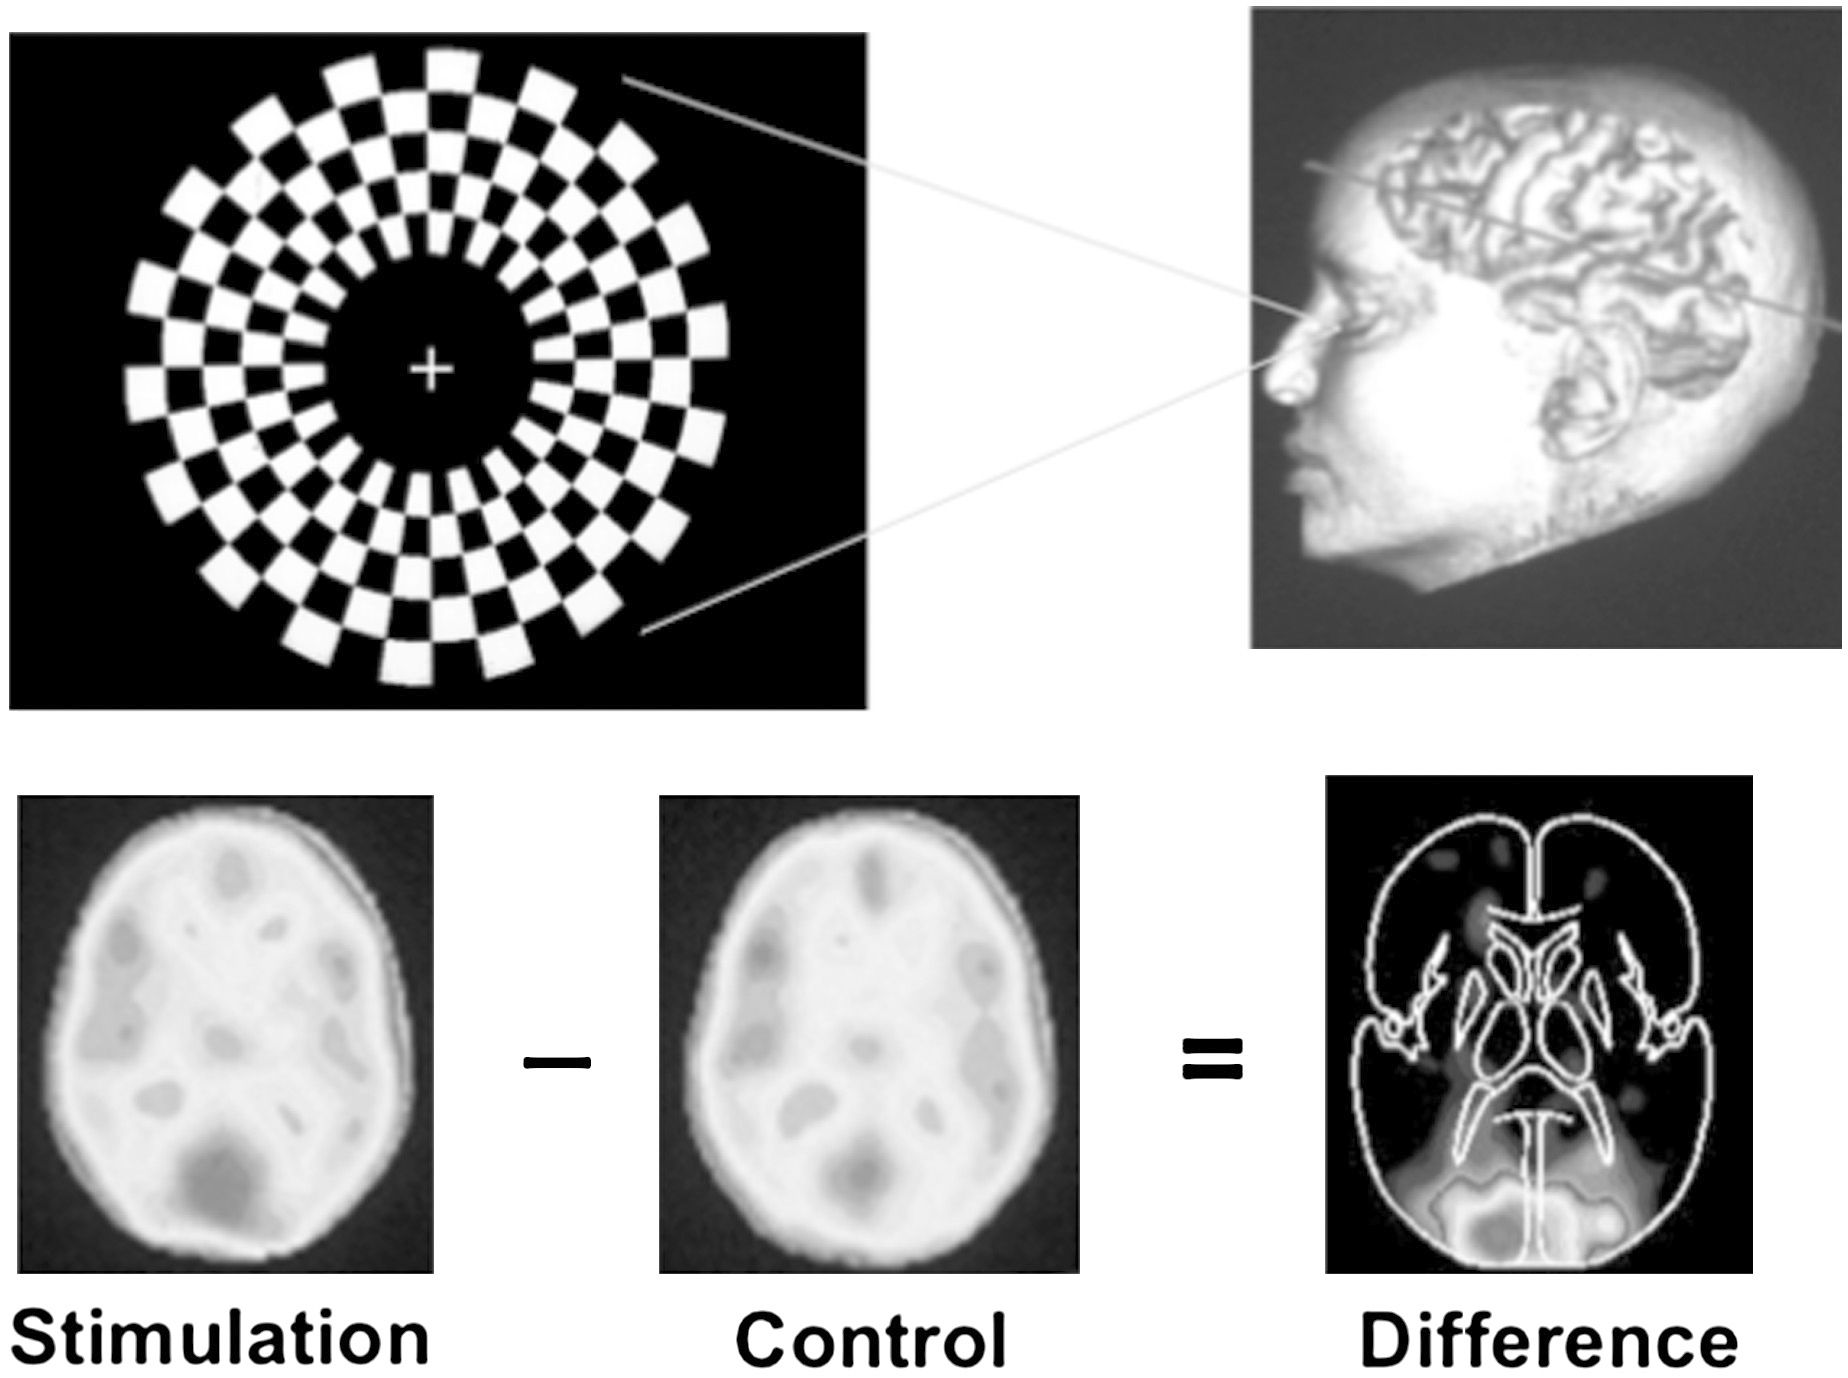
\includegraphics[width=3.67012in,height=2.7367in]{imgs/1.png}

Estimulação -- Controle = Diferença

Ilustração de técnica subtrativa. Dados coletados durante uma condição
de controle são subtraídos de dados coletados durante a realização da
tarefa de interesse.}\footnote[10]{Figura extraída de Roskies (2010). Cortesia
de Adina Roskies e Marcus E. Raichle.}
\end{center}

As áreas designadas como ativas são obtidas por ``subtração'' (Figura
2.1). Esquematicamente: sinais \versal{BOLD} gerados durante a tarefa T1 (a
condição de controle) indicam atividade nas áreas do cérebro B1 e B2;
supõe"-se que eesas áreas estão ``associadas'' aos processos
neurobiológicos ``subjacentes'' a T1. Sinais \versal{BOLD} gerados ao realizar a
tarefa experimental T2 demonstram aumento ou diminuição de atividade em
B1 e B2 e/ou ``ativação'' de novas áreas. O resultado experimental é
obtido subtraindo os dados de T2 e T1 (ou ``contrastando'' as
condições). Mesmo que as áreas ``ativadas'' assim identificadas
representem correlações, argumenta"-se que elas ``subjazem'' ou
``sustentam'' as funções envolvidas na tarefa, no sentido de constituir
seus ``substratos'' ou ``bases'' anatômicas e fisiológicas (Schleim e
Rosier, 2009).

Embora no começo do século \versal{XXI} a variedade de técnicas subtrativas
houvesse se tornado mais ampla que esse paradigma ``clássico'', elas
pressupõem os mesmos princípios e premissas que levaram a críticas
similares (Roskies, 2010, p.~638). Debates em torno a esses princípios e
premissas têm acontecido a níveis altamente técnicos e teóricos (ver,
por exemplo, Coltheart, 2006; Hardcastle e Stewart, 2002; Roskies, 2009,
2010; Van Orden e Papp, 1997). Um ponto especialmente relevante para
nossa discussão diz respeito à possibilidade de atribuir função ou
significado aos resultados. A neuroimagem, com certa frequência,
pressupôs que o cérebro é modular e que, portanto, a localização fornece
informação sobre funções mentais. Várias fontes de evidência, incluindo
a própria neuroimagem quando revela padrões replicáveis e ativações
confiáveis, demonstram que o cérebro realmente tem um determinado grau
de especialização funcional. Ao mesmo tempo, embora não equipotencial, o
cérebro é altamente plástico, interconectado e integrado. É
caracterizado por uma ``densidade causal'': isto é, qualquer tarefa
provavelmente terá efeitos por todo o cérebro, e ``há uma trilha causal
entre mudanças em qualquer variável explicativa e qualquer outra
variável'' (Klein, 2010, p.~269). Além disso, diferentes estados neurais
podem produzir o mesmo estado mental, como diferentes estados mentais
possuem os mesmos correlatos neurais (uma característica semelhante ao
que os filósofos denominam de ``múltipla realizabilidade''; Bickle,
2013). Considerando que B1 e B2 também são ativos em T2, a neuroimagem
não pode discriminar a função das várias ativações nem fornecer a base
para interpretar ativação modificada ou nova além de constatar uma
``associação'' entre elas e a tarefa experimental. Por isso, a
neuroimagem não poderia responder à pergunta: ``E daí?''.

Em defesa do método subtrativo, tem sido ponderadamente observado que os
resultados de neuroimagens, dificilmente significativos em si, não são
ou pelo menos não deveriam ser considerados de forma fragmentada e
isolada (Roskies, 2010; Rugg e Thompson"-Schill, 2013). Ao invés disso,
esses resultados precisam ser interpretados a partir de uma
``triangulação'' com referência a outros resultados do mesmo tópico,
outros experimentos de escaneamento e a informações de outros tipos,
tais como aqueles obtidos por outros métodos (por exemplo, na psicologia
ou neurofisiologia). Uma abordagem multimodal torna"-se, então,
indispensável. Até recentemente, tal abordagem teve um papel mínimo nas
neurodisciplinas, mas deveria ser, à princípio, benéfico. Porém, ir além
dos verbos comumente usados (``sustentar'' e assim por diante) para
descrever o papel de estruturas e circuitos relacionados à função ou
tarefa escolhida daria às neurodisciplinas a capacidade de dizer algo
relevante sobre seus tópicos?

Os resultados obtidos até agora sugerem que isso é improvável e que a
pesquisa reforçará o problema da múltipla realizabilidade aprofundando o
desafio de interpretar correlatos neurais. Por exemplo: cada pessoa tem
um ``perfil de conectividade'' que a distingue, ``independentemente de
como o cérebro é usado durante o escaneamento'' (Finn et al., 2015). De
modo similar, ao contrário do que reza a lenda, embora haja diferenças
sexuais no cérebro, principalmente atribuídas à exposição a hormônios na
vida perinatal (McCarthy, 2015), os cérebros não têm formas masculina e
feminina. Na verdade, a maioria dels são ``mosaicos'' únicos de
características, ``algumas mais comuns em mulheres em comparação com
homens, outras mais comuns em homens em comparação com mulheres, e
algumas comuns em mulheres e homens'' (Joel et al., 2015). Portanto,
embora ``as imagens do seu cérebro sejam fundamentalmente você'' (Finn,
2015), você não é fundamentalmente a imagem do seu cérebro.

As discussões sobre os usos e abusos das neuroimagens, especialmente em
contextos neurodisciplinares, não diminuíram. Em 2014, o Hastings
Center, uma instituição protagonista de bioética, dedicou seu relatório
técnico a avaliar a neuroimagem funcional. Nele, Martha Farah, uma
neurocientista cognitiva e figura de liderança em neuroética, investigou
sistematicamente as críticas feitas à neuroimagem e concluiu que, embora
cada uma delas tivesse uma ``dose de verdade'', todas elas também podiam
ser refutadas. Farah argumenta que um sinal \versal{BOLD} não é uma medida direta
da atividade cerebral, e não sabemos a quais aspectos da atividade
neural ele corresponde. Mas a relação entre os dois é suficientemente
forte para tornar a \versal{IRM}f uma ferramenta útil. Imagens, sejam gráficos ou
mapas, de fato são fabricadas, mas não inventadas. Embora a \versal{IRM}f diga
respeito à localização, mas não se trata de localização pela localização
em si, e a maior parte da investigação em neuroimagem não é motivada por
ela. (Essa pode ser uma generalização acurada em seus muitos campos de
aplicação, mas as neurodisciplinas parecem ser uma exceção.) Subtração?
Sim, inicialmente, a neuroimagem pressupôs módulos independentes de
contexto, de tal maneira que ``um processo cognitivo A terá a mesma
representação neural seja ele acompanhado por processos cognitivos B, C,
D ou E'' (Farah, 2014, p.S23). Mas demais abordagens, como a análise de
conectividade funcional, deveriam permitir à \versal{IRM}f transcender essa
limitação.

A pesquisa com neuroimagens tem sido criticada pelo uso de ``inferência
reversa'', ou seja, tentativas de inferir a presença de processos
mentais específicos a partir de ``ativações'' detectadas nas áreas
supostamente correspondentes (Poldrack, 2008). Ou seja, se há uma
ativação na área B1, então o processo mental M1 está acontecendo. Se
houvesse uma correspondência de um para um entre regiões cerebrais B e
esses processos M, seria possível inferir quais Ms estão acontecendo ao
identificar Bs ativos. Contudo, (conforme mencionado anteriormente)
visto que processos psicológicos utilizam diversas regiões cerebrais, e,
além disso, como uma única região cerebral normalmente está envolvida em
múltiplos processos, tal inferência não é possível. Farah (2014, S24)
argumentou que, com as devidas cautelas e informações provenientes de
processos de manipulação e observação de ativação cerebral, a inferência
reversa pode ser legítima. Se a realização de uma tarefa T envolvendo
processo mental M consistentemente ``ativa'' a região B do cérebro,
então a ativação de B pode indicar que M está acontecendo. Ainda que
tais inferências não sejam o objetivo da pesquisa neurodisciplinar, elas
auxiliam, como observa Poldrack (2008, p.~224) para ``orientar estudos
comportamentais ou de neuroimagem subsequentes, ao invés de serem um
meio direto de interpretar resultados de escaneamentos''.

Farah está correta em enfatizar que (também mencionado acima) muitos dos
problemas da \versal{IRM}f (inferência reversa, ambientes experimentais altamente
artificiais, pequenas amostras, baixa confiabilidade, confiabilidade
fraca e significado estatístico exagerado) são compartilhados por outras
áreas da pesquisa científica, e, ainda, que há uma diferença entre
criticar aplicações específicas e a ``crítica no atacado'' da
neuroimagem. Esta última diz respeito ao próprio método, lançando
dúvidas ``sobre as conclusões de qualquer pesquisa realizada com
escaneamento, não importando quão bem concebida e cuidadosamente
executada'' (Farah, 1914, p.S28). Essa posição indiscriminada certamente
seria injusta, e não há dúvida de que, desde o começo da onda das neuroX
nos anos 1990, um enorme avanço foi realizado para superar desafios
metodológicos e técnicos. Ainda assim, as carências congênitas das
neuroX não estão na qualidade do projeto e da execução dos experimentos,
mas em sua adequação aos objetos que alegam estar estudando.
Exemplificaremos isso em seguida.

É revelador a tamanha autoconfiança presente nas neurodisciplinas a
ponto de que um tópico tão sensível como esse não seja estudado. Em um
artigo de 1999 intitulado ``If Neuroimaging Is the Answer, What Is the
Question?'', o psicólogo cognitivo de Harvard Stephen Kosslyn duvidou
que processos mentais pudessem em algum momento serem melhor entendidos
quando se observa quais pontos neurais são ``ativados'' durante a
realização de uma tarefa. Ao contrário, o seu argumento é que se deve
começar com questões que inspiram tarefas experimentais de um modo a
usufruir da força das técnicas de escaneamento. Embora Kosslyn (1999)
estivesse refletindo sobre trabalhos realizados principalmente no começo
dos anos 1990, sua pergunta continua sendo mais atual do que nunca.
Quase vinte anos depois da publicação do artigo, e após considerável
populaização e incerteza, as neurodisciplinas apresentam sinais
evidentes de refinamento metodológico e teórico. Ao mesmo tempo, ainda é
necessário perguntar se os pressupostos e abordagens das neuroX são
adequados aos objetivos, questões e objetos que elas mesmo delimitam. A
resposta, como sugere nossos estudos de caso, é que não são.

\section{As neurodisciplinas da cultura}

A maioria das neurodisciplinas almeja capturar o que há de comum na
heterogeneidade de comportamentos e experiências --- em outras palavras,
processos neurobiológicos universais que são ``modulados'' por fatores
contextuais. Em contraste, as neurodisciplinas da cultura, como
neuroantropologia e neurociência cultural, se concentram menos no que é
comum e mais na diferença, isto é, naquilo que dá às culturas sua
especificidade e em como a cultura é ``gravada'' no cérebro. Como todas
as disciplinas do \emph{neuro}, elas tentam produzir suas explicações a
partir do conhecimento sobre o cérebro. Porém, são particularmente
atentas em enfatizar a ``enculturação'' do cérebro e as
\emph{interações} de cultura e cérebro. Assim, oferecem uma oportunidade
de estudar como a noção de cultura opera em uma estrutura construída
para examinar processos neurobiológicos transculturais.

Os editores de \emph{The Encultured Brain}, um livro que se apresenta
como ``uma introdução à neuroantropologia'', afirmam que o projeto da
disciplina consiste em ``estudar diferentes sistemas neurais
empiricamente, compreender como se desenvolvem as capacidades neurais e
documentar quais fatores biológicos e ambientais moldam sua realização''
(Downey e Lende, 2012, p. 24). Esse projeto tem sido considerado parte
de uma ``mudança instigante'' em direção à uma antropologia biológica
mais ``integrada'', na medida em que demonstra ``que a antropologia pode
oferecer à neurociência exemplos contextuais de como a enculturação pode
ajudar a explicar diferenças no funcionamento do cérebro, enquanto a
neurociência oferece à antropologia evidências diretas do papel da
neuroplasticidade na dinâmica social e cultural'' (MacKinnon, 2014,
p.~357). \emph{The Encultured Brain} alega romper com noções anteriores
de cultura:

\begin{quote}
Por muito tempo, os antropólogos se concentraram na cultura como um
sistema de associações simbólicas, sinais públicos ou significado
compartilhado. Mas, do ponto de vista do sistema nervoso, padrões de
variação em diferentes grupos também incluem significativas
características inconscientes e não simbólicas, como padrões de
comportamento, reação automática, habilidades e vieses perceptuais. A
perspectiva neuroantropológica propicia mais espaço para refletir as
razões pelas quais todos os tipos de cognição podem não operar de modo
idêntico, e como formas não cognitivas de enculturação neural podem
influenciar pensamento e ação. (Downey e Lende, 2012, 37).
\end{quote}

Em outras palavras, a cultura não tem a ver apenas com representações
compartilhadas, mas também com ``condicionamentos compartilhados do
sistema nervoso''. Isso pode parecer autoevidente, já que é improvável
que possa haver padrões compartilhados de comportamento, sejam
simbólicos ou automáticos, na ausência de alguns processos cerebrais
compartilhados. Porém, para os autores citados, são as ``implicações''
desse princípio que parecem ``óbvias''.

De acordo com Downey e Lende, ``as razões predominantes para que a
cultura se torne corporificada (\ldots{}) é que a neuroanatomia inerentemente
torna a experiência material'' (p.~37). A observação trivial de que ``sem
mudança material no cérebro, fatores como aprendizado, memória,
maturação e mesmo trauma não poderiam acontecer'' os leva à declaração
aparentemente significativa de que ``conceitos e significados culturais
se tornam anatomia neurológica'' (p.~37). Essa lógica, como dizem os
próprios autores, é óbvia. As questões pertinentes são se, ou em que
sentido, estudar mudanças no cérebro aumenta significativamente a
compreensão de cultura para além de reiterar que há processos
neurobiológicos envolvidos, e, ainda, como a noção de \emph{cultura}
opera na estrutura conceitual e metodológica do \emph{neuro}.

Essas problemáticas podem ser discutidas de dois formas, pelo menos. Por
um lado, em relação à pesquisa propriamente dita, podemos perguntar:
como as neurodisciplinas da cultura traduzem sua ênfase na
``bidirecionalidade'' cérebro"-cultura em estratégias investigativas
concretas, e quais são seus resultados empíricos? Por outro lado, essas
disciplinas podem ser analisadas em relação a seus valores implícitos e
epistemológicos. A despeito da insistência nos processos bidirecionais
que inserem o cérebro na cultura, e a cultura no cérebro, as
neurodisciplinas da cultura geralmente afirmam o primado ontológico do
cérebro e consideram os grupos humanos que constituem culturas como uma
``comunidade de cérebros'' (Domínguez Duque, 2015, p.~292). Tal premissa
transforma a cultura, independetemente de como é definida, em um fator
externo que ``molda'', ``influencia'' e ``tem impacto'' na atividade
neural, seu funcionamento e processos. A utilização espontânea desses
verbos causativos é sintomática da forma como as neurodisciplinas da
cultura abordam seu objeto (Gutchess e Goh, 2013; outras referências são
dadas mais adiante). Diante disso, qual é a consequência para essas
disciplinas e para o próprio conceito de cultura?

\section{Neurologizando a cultura}

Como as demais neurodisciplinas, aquelas que lidam com a cultura
passaram, em poucos anos, de um grupo informal de acadêmicos com
interesses em comum para disciplinas com nomes próprios e artigos na
Wikipedia, instituições profissionais, periódicos, sociedades,
colóquios, eventos educativos, blogs e sites na internet, programas e
alunos de graduação. Números especiais de periódicos, não
especificamente dedicados a elas, destacam as sinergias entre essas
novas disciplinas e campos mais bem estabelecidos. Assim, a neurociência
cultural tem sido objeto de edições especiais das revistas
\emph{Psychological Inquiry} (2013), \emph{Social Cognitive and
Affective Neuroscience (}2010), \emph{Asian Journal of Social Psychology
(}2010) e \emph{Progress in Brain Research} (2009). O \emph{Handbook of
Social Neuroscience} oferece um panorama geral da área (Chiao, 2011), e
o volume coletivo \emph{Cultural and Neural Frames of Cognition and
Communication (}Han and Pöppel, 2011) inclui diversas contribuições da
disciplina. Quanto à neuroantropologia, os apelos para tal empreitada
surgiram, pela primeira vez, no final dos anos 1970. A palavra foi
primeiramente empregada no começo dos anos 1990 e apareceu em obras de
referência de antropologia em meados da década (Marcus, 1997; Downey,
2012a). Em 2012, mesmo ano do lançamento de \emph{The Encultured Brain},
os periódicos \emph{Anthropological Theory} e \emph{Annals of
Anthropological Practice} dedicaram edições especiais à
neuroantropologia.

Por sua vez, o termo ``neurociência cultural'' aparece impresso pela
primeira vez em 2007, em um capítulo do \emph{Handbook of Cultural
Psychology}. Foi definida então como ``uma área de pesquisa que estuda
variação cultural em processos psicológicos, neurais e genômicos como um
meio de articular a inter"-relação desses processos e as propriedades
emergentes (Chiao e Ambady, 2007, p.~238). Os neurocientistas culturais,
evidentemente, reconhecem que fatores sociais oferecem mais que
``interesse mínimo'' para compreender o cérebro e os processos
comportamentais (Zhou e Cacioppo, 2010). Ao mesmo tempo, considerando
que o nível de análise sociocultural é por si só insuficiente, destacam
a \emph{interdisciplinaridade} de sua empreitada e a
\emph{bidirecionalidade} dos processos que estudam, e falam de um
``co"-construtivismo biocultural'' e ``determinismo múltiplo'' ou
``recíproco'' (Zhou e Cacioppo, 2010). Neurocientistas culturais
sustentam que valores, práticas e crenças ``moldam e são moldadas por
mente, cérebro e genes'' e que o estudo da ``variação cultural em
processos mentais, neurais e genômicos'' constitui um meio de
``articular a relação bidirecional desses processos e suas propriedades
emergentes'' (Chiao e Cheon, 2012, p.~288; Chiao et al., 2013; Kim e
Sasaki, 2014).

Embora a noção de que o comportamento complexo ``resulta da interação
dinâmica de genes e do ambiente cultural'' não seja exatamente nova, a
neurociência cultural supostamente representa ``uma nova abordagem
empírica para demonstrar interações bidirecionais entre cultura e
biologia, integrando teoria e métodos de psicologia cultural,
neurociência e neurogenética'' (Chiao e Cheon, 2012, p.~289). Essa
perspectiva visa ``explicar um determinado fenômeno mental em termos do
produto sinérgico de acontecimentos mentais, neurais e genéticos''
(p.~289) e alega ter ``implicações potenciais'' não apenas para
psiquiatria, negócios e tecnologia, mas também para políticas públicas
globais de saúde, globalização, imigração e ideologia interétnica
(Chiao, 2009b; Denkhaus e Bös, 2012). No que tange à pesquisa, os
neurocientistas culturais são motivados por duas questões ``ainda não
respondidas'': como características culturais ``moldam'' neurobiologia e
comportamento? E como mecanismos neurobiológicos ``facilitam a
emergência e a transmissão de características culturais''? (Chiao et
al., 2010, p.~356).

Neuroantropologia e neurociência cultural não representam a primeira
tentativa de abordar a cultura com ferramentas neurocientíficas. Desde o
começo da década de 1990, a neurociência cognitiva foi incorporada ao
estudo de comportamento interpessoal e social. A ``neurociência social''
surgiu no final daquela década (ver Cacioppo e Berntson, 1992 para a
utilização inicial do termo) e, em 2005, já havia sido publicado um
manual de ``leituras fundamentais'' (Cacioppo e Berntson, 2005). O campo
deriva de descobertas na psicologia transcultural que mostram como a
cognição social e o comportamento dependem do contexto sociocultural.
Dessa forma, combina neuroimagem, ciência cognitiva e psicologia social
para estudar a ``representação'' neural da interação social bem como os
``substratos'' neurais de processos sociais (Han e Northoff, 2008; Zhou
e Cacioppo, 2010). Os periódicos \emph{Social Neuroscience} e
\emph{Social Cognitive and Affective Neuroscience} foram lançados em
2006; em 2008, foi criada a Social and Affective Neuroscience Society
``comprometida com a pesquisa da base neural dos processos sociais e
afetivos'', seguida, em 2010, pela Society for Social Neuroscience,
voltada para apoiar ``o campo acadêmico interdisciplinar dedicado a
compreender como sistemas biológicos implementam processos e
comportamento sociais, e como essas estruturas e processos sociais têm
impacto no cérebro e na biologia''\footnote[11]{\textless{}\emph{https://s4sn.org/}\textgreater{}.}. O periódico
\emph{Culture and Brain} foi fundado em 2013, dedicado às ``diferenças
culturais na atividade neural'' e à ``constituição mútua de cultura e
cérebro'' (Han, 2013).

As neurociências culturais, afetivas e sociais se sobrepõemem grande
medida umas às outras, bem como à neuroantropologia e à neuroimagem
transcultural (Domínguez Duque et al., 2009; Han e Northorff, 2008;
Lende e Downey, 2012a). Por exemplo, rótulos como ``neurociência
sociocultural'' são criados para sublinhar interconexões (Wajman et al.,
2015). Ao mesmo tempo, essas disciplinas emergentes se engajam em
dinâmicas de diferenciação. Particularmente, os neuroantropólogos têm
enfatizado as diferenças entre sua abordagem e aquela da neurociência
cultural (Domínguez Duque, 2012; Lende e Downey, 2012a). Na sua leitura,
enquanto que a neurociência cultural almeja, sobretudo, oferecer
explicações no nível do cérebro, a neuroantropologia busca combinar
essas explicações com uma perspectiva etnográfica. Logo, a
neuroantropoligia se encontra ``em melhor posição para se deslocar entre
os domínios neural, fenomênico e cultural'' (Domínguez Duque, 2012,
p.~22) e testar hipóteses neurocientíficas ``contra a realidade do que as
pessoas realmente fazem, dizem e experimentam'' (Downey e Lende, 2012,
p.~42). Em suma, a etnografia deveria ser capaz de propiciar ``acesso
empírico'' às formas pelas quais processos sociais e culturais moldam o
funcionamento, o significado e o comportamento cerebrais (p.~42). Alguns
neuroantropólogos demonstraram preocupação com possíveis vieses
culturais na pesquisa e, por isso, demandaram maior conscientização das
circunstâncias históricas, sociais e políticas nas quais os experimentos
são realizados (Domínguez Duque et al., 2010); já outros autores
consideram a interface entre antropologia e as neurociências um modo de
fazer antropologia experimental (Roepstorff e Frith, 2012).

Resumindo, existe um conjunto de disciplinas \emph{neuro} destinadas a
compreender como o cérebro ``media'' interações sociais e culturais e
produz emoção e cognição. A questão é como e se essas questões e
declarações programáticas podem se traduzir em resultados de pesquisa
capazes de ir além de generalidades como ``as práticas culturais se
adaptam a restrições neurais, e o cérebro se adapta à prática cultural''
(Ambady e Bharucha, 2009, p.~342), generalidades essas que apenas
reiteram a premissa do campo.

\section{Causas, correlações, plasticidade}

À medida em que a neuroimagem, supostamente, revela ``quão
`profundamente' a cultura pode penetrar no cérebro humano'' (Kitayama
e Park, 2010, p. 124), tem sido o método preferido para estudar
diretamente o cérebro ``aculturado''. Todavia, observando que a
neuroantropologia toma seus principais conceitos e questões da
antropologia cultural, ela enfatiza o trabalho de campo como sua base
empírica e, consequentemente, tende menos a usar neuroimagens, que
demandam um ambiente experimental. Por isso, a maioria dos estudos
neuroantropológicos se limita a citar pesquisas cerebrais e justapô"-las
a outros tipos de materiais extraídos diretamente do estudo de ambientes
e situações culturais, com a premissa de que tal justaposição demonstra
o impacto dessas situações no cérebro ou a ``interação'' de cultura,
cérebros e experiência (ver, por exemplo, \emph{The Encultured Brain}
{[}Lende e Downey, 2012a{]} ou a edição especial ``Neuroantropology and
Its Applications'', \emph{Annals of Anthropological Practice} 36, 2012).
Em suma, a ``neuroantropologia'' designa basicamente o nome de uma
potencial estrutura que aparentemente possui escasso impacto no trabalho
antropológico concreto. Um estudo sobre a antropologia dos tratamentos
de manutenção de opiáceos para a adição pode ser redescrito como
``neuroantropologia'', e seu objeto como ``as políticas neuroeconômicas
e neurorraciais de fármacos opiáceos'' (Hansen e Skinner, 2012). De modo
similar, simplesmente acoplando o rótulo ``neurocognitivo'' às
habilidades envolvidas que etnografias do rugby ou da capoeira se tornam
casos de neuroantropologia (Downey, 2012b; 2012c). A operação de
renomear é puramente cosmética e uma boa jogada de marketing, mas não
gera ganhos metodológicos, empíricos ou conceituais.

Em contraste com a neuroantropologia, a neurociência cultural usa
neuroimagens de modo tão sistemático que é frequentemente descrita como
``neuroimagem cultural''. Essa descrição não implica dizer que a
neuroantropologia se beneficiaria se valendo da neuroimagem, mas sim que
métodos de escaneamento têm sido, até agora, o principal modo de
realizar trabalho empírico para além de meramente justapor o
neurobiológico e o cultural. A questão é se essas neurodisciplinas
satisfazem o \emph{a priori} o objetivo lançar novas luzes sobre a
cultura.

Em relação às neuroimagens, a distinção entre neuroantropologia e
neurociência cultural é coerente com suas raízes conceituais e
disciplinares na antropologia cultural e na psicologia cultural,
respectivamente. A psicologia cultural é realmente a ``disciplina mãe''
da neurociência cultural'' (Denkhaus e Bös, 2012) --- só que de uma
forma que implica pouco mais que substituir a ``mente'' da \emph{psi}
pelo ``cérebro'' da \emph{neuro}. De fato, o antropólogo da Universidade
de Chicago, Richard Shweder (1991, p.~72), definiu a psicologia cultural
como o estudo de ``como tradições culturais e práticas sociais regulam,
expressam e transformam a psique humana, resultando menos em uma unidade
psíquica para a humanidade do que em divergências étnicas em mente, \emph{self}
e emoção''. Se substituirmos \emph{psique humana} por \emph{cérebro
humano} e \emph{unidade psíquica} por \emph{unidade neural}, e depois
acrescentarmos ``cérebro'' à localização das divergências étnicas,
obtemos uma descrição precisa da neurociência cultural.

Esse campo supõe que ``compreender as \emph{influências} culturais e
genéticas no funcionamento do cérebro provavelmente é a chave para
articular uma teoria psicológica mais adequada'' (Chiao, 2009b, p.~290).
A busca por ``influências'' é reforçada pela premissa de que ``o
comportamento humano é \emph{resultado} da atividade neural'' e pela
posterior inferência de que a variação comportamental nas culturas
``provavelmente \emph{emerge} da variação cultural em mecanismos neurais
subjacentes a esses comportamentos (Chiao, 2009b, p.~290, ênfase nossa;
ver também Chiao e Cheon, 2012, p.~289). A partir do uso do
``provavelmente'' de forma vaga, o raciocínio pressupõe uma direção e
uma hierarquia de causas, da genética e o cérebro até a mente e a
cultura. Métodos de neuroimagem e genômica para ``mapear'' processos
neurais e genes ``para'' processos neurais, mentais e culturais produzem
correlações, mas elas são apresentadas de um ponto de vista causal, o
que é reforçado pela crença de que características culturais constituem
adaptações evolucionárias (Chiao e Blizinsky, 2010).

A tensão entre resultados correlacionais e argumentações causais, bem
como a existência de uma hierarquia epistêmica implícita, prejudicam o
apelo da neurociência cultural à sinergia e à bidirecionalidade.
Posteriormente nos deteremos em pesquisas relevantes, mas vejamos por
ora um exemplo da afirmação de que valores, práticas e crenças culturais
têm ``impacto no comportamento humano'' ou que a ``dimensão cultural''
de \emph{individualismo"-coletivismo} (um dos temas preferidos da
psicologia cultural) ``afeta uma grande variedade de processos mentais
humanos no nível comportamental'' e ``modula reações neurais e
eletrofisiológicas'' (Chiao, 2009b, p.~291 e 295). Esse tipo de
declarações possui um raciocínio circular. Por um lado, a ``dimensão''
cultural inclui, por definição, processos mentais e comportamentais que
necessariamente têm correlação com alguma característica do
funcionamento do cérebro. Por outro lado, a própria dimensão cultural é
definida, pelo menos em parte, com base nos processos mentais e
comportamentais que ela supostamente ``afeta''.

A cultura ``influencia'' o funcionamento do cérebro, ``modula''
mecanismos neurais e ``molda'' sistemas neurais (ibid., p. 291). Assim,
indíviduos que vivem na cultura X podem desenvolver ``mecanismos neurais
distintos''. Todavia, esses mecanismos podem ser ``subjacentes'' a
comportamentos idênticos aos observáveis na cultura Y, na qual se
correlacionam com outros processos neurais (p. 290). A neurociência
cultural analisou esses efeitos relacionando com emoções (ao oferecer
``evidências de que a cultura influencia o modo como as pessoas deduzem
estados emocionais'', p. 296), com percepções interpessoais (mostrando
que indivíduos de culturas igualitárias \emph{versus} culturas
hierárquicas apresentam maior atividade mesolímbica para exemplos
dominantes \emph{versus} exemplos faciais; Freeman et al., 2009), e com
cognição social (demonstrando que valores culturais, em vez de filiação
étnica, ``modulam a reação neural durante a avaliação pessoal''; Chiao,
2009b, p.~297). A disciplina estuda uma ampla gama de processos
psicológicos, do processamento visual e semântico (Goh et al., 2010;
Gutchess et al., 2010) ao medo (Chiao et al., 2008), à empatia (Cheon et
al., 2011) e à autorrepresentação (Kitayama e Park, 2010; Mrazek, Harada
e Chiao, 2014). A explicação básica é sempre a mesma: a cultura molda a
atividade de alguma parte do cérebro, que, por sua vez, guia o
comportamento.

Os neurocientistas culturais consideram suas descobertas sustentadas
pela existência da neuroplasticidade (a capacidade do cérebro de mudar
como resultado da experiência) e sua principal consequência teórica, a
qual desafia a crença de que as funções do cérebro têm localizações
fixas e que o cérebro é maleável apenas em períodos críticos rigidamente
limitados. Celebrada, conforme visto anteriormente no Capítulo 1, como
uma descoberta revolucionária e imediatamente adotada por um amplo
espectro de indivíduos com algum interesse específico, desde vendedores
de malhação cerebral até filósofos e psiquiatras, cientistas políticos e
especialistas em reabilitação, a neuroplasticidade supostamente confirma
que as diferenças culturais no nível neural residem em padrões de
conectividade. O envolvimento sustentado em atividades culturais,
compreendidas como participação repetida em comportamentos rotineiros,
resulta em diferentes padrões de ativação cerebral e modificações
funcionais e estruturais (ver Hanawaka et al., 2003, para especialistas
japoneses em ábaco, ou Maguire et al., 2000, para motoristas de táxi de
Londres). Dessa forma, a plasticidade cerebral pode ser descrita como a
característica que permite a interação do cérebro e cultura nos três
níveis interrelacionados de valores explícitos, convenções e rotinas;
roteiros de ação socialmente partilhados; e idiossincrasia individual.
Assim, a neruoplasticidade explica as diferenças neurais interculturais
como consequência de prática e experiência.

\section{Práticas investigativas}

A neurociência cultual seguiu duas estratégias. Uma, o ``mapeamento
cultural'', que implica ``determinar quais processos cognitivos ou
neurais variam nas culturas sem determinar se as diferenças são
aprendidas ou inatas'' (Ambady e Bharucha, 2009, p.~342). Por exemplo, ao
realizar tarefas numéricas, anglófonos nativos apresentaram maior
ativação em áreas do cérebro ``associadas'' ao processamento de
linguagem, enquanto que sinofalantes nativos apresentaram ativação mais
intensa em áreas do cérebro ``associadas'' ao processamento
visual"-espacial (Tang et al., 2006). A descoberta é hipoteticamente
atribuída a exposição à diferentes padrões visuais. Uma maior atividade
pré"-motoras nos chineses ``poderia ser atribuída'' à natureza
visual"-espacial de seu idioma, ao passo que a ativação de áreas de
linguagem nos anglofalantes sugere que ``a recuperação de fatos
matemáticos pode ser mediada por processamento fonológico'' (Ambady e
Bharucha, 2009, p.~342-343). A segunda estratégia, denominada ``análise
de fontes'', visa determinar ``a fonte ou causas'' de mapeamentos
culturais, incluindo semelhança ou diferença genética, aprendizado
cultural ``mediado pela plasticidade do cérebro'' e o grau de
similaridade entre ambientes culturais. Essa estratégia tem sido menos
empregada do que à primeira, ``mas novas tecnologias prometem'' um
``avanço rápido'' (p. 343, 344). Até 2016, essa promessa parecer se
manter apenas de maneira programática.

Em contrapartida, os neuroantropólogos se veem situados de forma
privilegiada para explorar a bidirecionalidade cérebro"-cultura e (como
mencionamos) adotam uma postura crítica diante da neurociência cultural.
Porém, eles também se concentram em como a cultura ``influencia'' ou
``muda'' o funcionamento e a estrutura do cérebro e como áreas cerebrais
``reagem a regularidades no fluxo de experiência cultural'' (Domínguez
Duque et al., 2009, p.~43). Esses teóricos saúdam como ``extraordinário''
o fato de que a cultura ``afeta'' não apenas o funcionamento do cérebro,
mas também sua estrutura (ibid., p. 60; ver também Domínguez Duque,
2012, p.~22). Como explica uma equipe de neuroantropólogos, o córtex
pré"-frontal ``é o primeiro a ser modificado ou construído pela
experiência cultural por ser a estrutura que \emph{lança} as fundações
da cultura'' (Domínguez Duque et al., 2009, p.~60- 61, ênfase nossa). A
noção de que o córtex pré"-frontal é \emph{constituído} pela cultura, ao
mesmo tempo em que é o maior responsável por \emph{gerá"-la}, vai além de
descrever a interação recíproca que se obtém em todos os níveis, de
corpo e mundo. Tal premissa destaca, assim, a assimetria fundamental das
neurodisciplinas da cultura. A defesa de que a cultura, como um conjunto
de atividades, incluindo formas de aprendizado, ``modifica'' o cérebro é
certamente fundamentada pela observação empírica. Em contraste, exceto
em sua interpretação mais fraca, a afirmação de que o córtex pré"-frontal
``lança'' as fundações da cultura formula um pressuposto ontológico. E é
justamente esse pressuposto que se reflete na forma como a pesquisa é
conduzida.

Observemos, por exemplo, um artigo frequentemente citado na área,
publicado em 2009 no periódico \emph{Human Brain Mapping}, e intitulado
``Neural Basis of Individualistic and Collectivistic Views of the
Self''. O objetivo do artigo é compreender como individualismo e
coletivismo ``modulam representações neurais subjacentes à cognição
social'' (Chiao et al. 2009, p.~2813). De acordo com estudos prévios,
indivíduos que defendem valores individualistas olham para si mesmos e
para os outros como indivíduos independentes e com características
pessoais estáveis. Em compensação, indivíduos que endossam ideais
coletivistas veem as pessoas como interconectadas e se descrevem como
imersas em um contexto social. Para tanto, os autores do artigo utilizam
a noção de estilo de autoimagem (\emph{self"-construal style} - \versal{SCS}, na
sigla em inglês), que foi usada para diferenciar as visões ocidental e
leste"-asiáticas do \emph{self}. Os autores não citam pesquisas
problematizando a capacidade de a autoimagem refletir a orientação
cultural à nível individual ou de mediar e explicar diferenças
transculturais (Levine et al., 2003).

Com base em trabalhos anteriores, os quais indicam que a atividade no
córtex pré"-frontal medial (\versal{CPFM}) ``reflete a base neural do
autoconhecimento (Chiao et al., 2009, p.~2814; Kelley et al., 2002), os
autores apresentaram a hipótese de que individualistas exibiriam uma
maior resposta a autodescrições gerais, enquanto que os coletivistas, a
autodescrições contextuais, na porção anterior rostral do \versal{CPFM}. Para o
estudo que originou o artigo ``Neural Basis of Individualistic and
Collectivistic Views of the Self'', vinte e quatro universitários
destros foram recrutados, doze japoneses de Nagoya e doze ``americanos
caucasianos'' de Chicago. Os estudantes receberam setenta e dois
estímulos, respectivamente em japonês e inglês: vinte e quatro
autodescrições gerais, vinte e quatro autodescrições contextuais e vinte
e quatro autodescrições em fonte grifada. Em comparação com os
coletivistas, durante as autoavaliações os individualistas exibiram
maior ativações no tálamo bilateral, putâmen direito, cúneo bilateral,
ínsula direita, cerebelo bilateral e giro frontal superior direito. Já
os coletivistas, por sua vez, apresentaram, durante a mesma tarefa,
maior ativação no giro temporal medial esquerdo. O estilo de
autoimagem, como definido após o escaneamento, interagiu de modo
estatisticamente significativo com ``o tipo de autoavaliação em reação
neural na região anterior rostral do \versal{CPFM}'', os giros para"-hipocampais,
giro temporal medial direito e giro occipital superior esquerdo (Chiao
et al., 2009, p.~2817).

Os resultados demonstraram que ``o processamento autorrelevante no \versal{CPFM}
varia enquanto função do {[}estilo de autoimagem{]}''. Indivíduos que
endossaram valores individualistas apresentaram maior ativação do \versal{CPFM}
durante autodescrições gerais, enquanto aqueles que endossaram valores
coletivistas apresentaram maior ativação do \versal{CPFM} durante autodescrições
contextuais. Nos dois casos, o aumento da atividade do \versal{CPFM} ``reflete o
papel que o \versal{SCS} desempenha em como o conhecimento sobre o \emph{self} é
formado, e possivelmente também estocado e acessado''. Os pesquisadores
concluíram, então, que ``o conhecimento das autorrepresentações do
próprio \emph{self} (\ldots{}) são culturalmente específicos no nível neural''. Além
disso, os autores especularam que a maior atividade no giro frontal
superior direito pode ``refletir evidência de um processamento
autorrelevante maior em individualistas em comparação com
coletivistas'', e, para tanto, solicitaram mais pesquisas para elucidar
como valores culturais ``afetam'' o processamento neural (Chiao et al.,
2009, p.~2819). Uma meta"-análise da pesquisa na área, publicadas entre
2003 e 2014, confirma que ``culturas do leste da Ásia estão associadas
ao aumento da atividade neural nas regiões do cérebro relacionadas à
inferência das mentes dos outros e à regulação das emoções, enquanto
culturas ocidentais estão associadas ao aumento da atividade neural nas
áreas do cérebro relacionadas à codificação da relevância pessoal e a
reações emocionais durante processos sociais cognitivos/afetivos'' (Han
e Ma, 2014, p.~283).

Esses tipos de estudos das ``bases'' neurais do individualismo e
coletivismo são característicos das neurodisciplinas em, pelo menos,
duas formas. Em primeiro lugar, os estudos ilustram o peculiar deslize
entre a formação de correlações estatísticas (aqui, a cultura funciona
como um determinante) e a identificação de ``bases'' ou ``fundações''
anatômico"-funcionais. Em segundo lugar, os resultados que poderiam ter
relevância são previsíveis sem neurociência ou neuroimagens. Os autores
do artigo ``Neural Basis of Individualistic and Collectivistic Views of
the Self'' chamam atenção para ``um aspecto intrigante'' de suas
descobertas: o fato de que os valores culturais dos participantes
(individualismo ou coletivismo), e não a afiliação cultural (ser
americano branco ou japonês nativo), ``modularam'' a reação neural
durante a avaliação pessoal (Chiao et al., 2009, p.~2819). Contudo, nos
contextos ocidental e leste"-asiático, dos quais eram originários os
sujeitos do estudo, as pessoas se ajustam à diversas exigências
ambientais, de forma que a cultura, definida a partir da afiliação
étnica ou nacional, não corresponde sempre ao comportamento individual.
Então, esses resultados não são de modo algum ``intrigantes''. Um dos
principais objetivos de um estudo desse cárater, como o que acabamos de
apresentar, é transmitir a premissa de que a cultura é baseada no
cérebro e, além disso, a crença de que um fenômeno se torna mais real em
virtude do seu correlato neural. A menos que esses pressupostos sejam
admitidos não há necessidade, então, da neurociência para compreender a
``natureza dinâmica dos valores culturais em indivíduos e grupos
culturais'' (p. 2819).

Neurocientistas culturais poderiam replicar que eles não apenas
corroboraram resultados das ciências sociais, mas ainda acrescentaram
algo essencial ao mostrar ``como valores culturais tão dinâmicos moldam
representações neurais'' (p.~2819). Entretanto, da mesma forma como não
conseguem demonstrar as ``bases'' neurais de valores ou posturas
culturalmente dependentes, os neurocientistas da cultura não conseguem
mostrar como valores ou posturas \emph{individuais} moldam o cérebro.
Evidentemente, ``valores, crenças e práticas culturais devem ser
importantes para o funcionamento do cérebro social'' (p.~2819). Essa
constatação, contudo, é assim por definição. Primeiramente, se justifica
porque qualquer coisa que organismos com cérebro fazem é relacionada à
função cerebral. Em segundo lugar, porque considerando que o ``cérebro
social'' diz respeito às regiões do cérebro envolvidas em compreender os
outros (Blakemore, 2008) e que a cognição social é, pelo menos nos
humanos, inseparável de formas culturalmente determinadas de interagir
com outros, a cultura é necessariamente ``importante'' para o cérebro
social. Nesses dois casos, o contrário constituiria uma descoberta
sensacional, quando não uma \emph{contradictio in adjecto}.

\section{Diversidade cultural como ``neurodiversidade''}

Por um lado, em relação ao seu significado para entender a cultura,
experimentos com neuroimagem recuperam no final o que colocam no começo,
especificamente a noção de que a cultura tem ``bases neurais''. Por
outro lado, a retórica da admiração, na qual descobertas são sempre
``intrigantes'' ou ``extraordinárias'', delata a persistência de uma
postura dualista. Celebrar o achado de que a ``cultura'', de algum modo,
``modifica a função cerebral implica imaginar ao menos duas dualidades:
cérebro e pessoa, cultura e indivíduo. Porém, como tem sido destacado
mesmo dentro da disciplina, ``não deveria ser surpreendente \emph{per
se} que exista uma diferença neural subjacente à diferença psicológica''
--- de fato, a existência dessa diferença é ``uma suposição axiomática''
da neurociência cultural, e não uma ``questão empírica'' (Freeman, 2013,
p.~26).

Os neurocientistas culturais, cujo estudo foi anteriormente apresentado,
relataram a ``influência de valores culturais em reações neurais no \versal{CPFM}
durante julgamentos pessoais, a despeito da ausência de diferenças no
nível comportamental'' e, assim, concluíram que seus resultados
``revelam uma vantagem de estudar valores culturais como \versal{SCS} no nível
neural'' (Chiao et al., 2009, p. 2819). A ``vantagem'' reside no
potencial de desvelar a afiliação cultural na ausência de um
comportamento observável. Ora, tal inscrição de valores culturais ``no
nível neural'' só poderia significar duas coisas. Uma é que a cultura,
incluindo crenças, normas e significados, está de algum modo
corporificada nos indivíduos, especificamente em seus cérebros,
pré"-reflexivamente moldando suas ações (Choudhury e Slaby, 2012a;
Gallagher e Zahavi, 2008; Noë, 2009). Outra é que o nível neural revela
uma verdade sobre os humanos como seres culturais que não pode ser
conhecida estudando práticas sociais e culturais. Ainda que as
declarações programáticas da neurociência cultural pareçam favorecer a
primeira interpretação, a sua prática materializa a segunda.

Um estudo recorrentemente citado sobre as ``Bases neurais da influência
cultural na representação do \emph{self}'' oferece outro exemplo dessa
perspectiva (Zhu et al., 2007; ver também as replicações em Ng et al.,
2010; Ray et al., 2010). Os autores usaram \versal{IRM}f para analisar a
atividade cerebral de sujeitos ocidentais e chineses enquanto eram
solicitados que julgassem se um determinado adjetivo era adequado para
descrever o \emph{self}, a mãe e o outro. julgavam atributos sobre si mesmos, a
sua mãe ou uma pessoa pública. Como outros pesquisadores no campo, os
autores começaram observando que, enquanto norte"-americanos e europeus
tendiam a ver o \emph{self} como independente, autônomo e separado dos outros,
asiáticos enfatizavam a interdependência e as interconexões. O desenho
do experimento era padrão: treze universitários chineses e treze
ocidentais foram escaneados enquanto se solicitava que julgassem os
mencionados adjetivos. Também foi pedido (como condição de controle
neutra) que avaliassem a tipologia em que as palavras eram escritas.

Os resultados alegaram oferecer evidência de uma distinção neural entre
o \emph{self} e pessoas íntimas para ocidentais, mas não para os chineses.
Assim, nos sujeitos chineses, ``julgamentos acerca da mãe'' geraram
atividade ampliada de \versal{CPFM} (comparada com ``outros julgamentos'' e a
condição neutra), de modo que ``a representação da mãe chinesa'' não
podia ser distinguida ``da representação do \emph{self} em termos de atividade
de \versal{CPFM}''. Esse resultado indicaria que enquanto os chineses ``usam'' o
\versal{CPFM} para ``representar'' tanto mãe quanto \emph{self}, a atividade de \versal{CPFM} em
sujeitos ocidentais corresponde a uma ``representação'' apenas do \emph{self}
individual (Zhu et al., 2007, p.~1314). De acordo com os autores, os
dados eram significativos para antropologia e neurociência porque
sugeriam ``que a cultura influencia a neuroanatomia funcional da
autorrepresentação'' e forneciam evidências de uma ``interação de
biologia e cultura para moldar mente e cérebro'' (1315).

À primeira vista, o estudo se localiza entre um construtivismo social
que reduz o papel da biologia à processos e práticas culturais e
sociais, e um reducionismo naturalista segundo o qual relações
interpessoais e culturais surgem no cérebro. Contudo, a não ser que se
assuma uma das duas posições e, logo, se engaje em uma forma de
dualismo, é difícil justificar experimentos caros apenas para constatar
como ``a cultura influencia a neuroanatomia funcional da
autorrepresentação'' ou ``processos cognitivos habituais são
acompanhados de processos neurais paralelos detectáveis
{[}\emph{sic}{]}'' (p.~1315-1314). O paradoxo reside no significativo
viés cartesiano por trás da ênfase explícita em interações recíprocas
cérebro"-cultura.

Como os autores explicam, a psicologia social demonstrou diferenças
comportamentais e cognitivas entre o \emph{self} ocidental e o asiático. Porém,
visto que a psicologia não afirmou ``se a cultura influencia os
mecanismos neurais relevantes'', mostra"-se ainda necessário buscar
evidências por neuroimagens de que o \emph{self} ocidental e o chinês
efetivamente diferem ``em um nível neural'' (p.~1313-1315). Assim, dois
polos foram unidos: a cultura, simultaneamente, ``afeta a estrutura
psicológica do \emph{self}'' e ``molda a anatomia funcional da
autorrepresentação'' (p.~1310). São dois os problemas com essa alegação.
Por um lado, correlações não expressam relações que possam ser
capturadas por verbos como ``afetar'' e ``moldar''. Por outro lado, a
utilização desses verbos revela uma visão peculiarmente abstrata e
mecânica da cultura. Contrariamente ao modo como são conceitualizadas
aqui, noções, posturas e práticas associadas ao \emph{self} são partes
integrais da cultura. Ou seja, estão entre as características
fundamentais que contribuem para que ela exista, e não algo que um
agente misterioso chamado ``cultura'' molda de fora.

Enquanto que a diversidade cultural é conceitualizada essencialmente
como uma forma de neurodiversidade, as definições experimentais e os
resultados da neurociência cultural podem se tornar parte de políticas
identitárias (Roepstorff, 2011, p.~40). Ao mesmo tempo, ao afirmar a
existência de diferenças entre \emph{selves} ``no nível neural'', a
neurociência cultural contribui para minimizar a diversidade dentro de
um grupo. Nos dois cenários (diferença interétnica e identidade
intragrupo), o cérebro recebe primazia ontológica. A mente é o que o
cérebro faz, e a cultura está incluída no processo. Uma das preocupações
mais sensível neste trabalho não é que a neurociência cultural pareça
sugerir que não existam valores universais (Begley, 2010), mas que
naturalize estereótipos culturais no laboratório (Choudhury, 2010;
Choudhury e Krmayer, 2009). Tem sido realizados apelos para
considerações mais nuançadas de fatores socioecológicos (Cheon et al.,
2013), mas até agora não foram incorporados de maneira sistemática no
trabalho experimental. Além disso, a neurociência cultural ainda deve
enfrenatar as consequências das complexas histórias intelectuais e
políticas ao escolher categorias como ``caucasiano americano'' (ver
Painter, 2010 para um panorama). De fato, como destacaram os críticos,
na prática, a neurociência cultural tende a classificar os sujeitos com
base na aparência exterior à custa das dimensões comportamental,
sociológica ou cultural. A disciplina tem ``uma compreensão de `cultura'
e `raça' que ainda apela a biologia, sangue e ancestralidade'' e,
portanto, parece reforçar ``o domínio ocidental em uma situação
pós"-colonial'' (Martinez Mateo et al., 2012, p.~160; 2013, p.~3).
Independentemente se a neurociência cultural é realmente tão
politicamente incorreta, a sua noção de ``cultura'' funciona como um
substituto de ``raça'' (Heinz et al., 2014).

\section{Da cultura para o cérebro}

É possível objetar que individualismo/coletivismo e autorrepresentação
são temas particularmente problemáticos ou então que nos limitamos a
investigações que alegam especificamente ser sobre ``bases neurais''
(para uma síntese, ver Zhu e Han, 2008). Afinal, pesquisas têm sido
realizadas sobre temas tao diversos como processamento perceptual
(Kitayama et al., 2003), modulação de atenção (Hedden et al., 2008),
linguagem (Tan et al., 2005; Lei, Akama e Murphy, 2014), música (Nan et
al., 2008), representação numérica e cálculo mental (Tang et al., 2006),
processos emocionais (Chiao et al., 2008), atribuição mental (Tang et
al. 2006) e autorrepresentação e consciência pessoal (Han e Northoff,
2008); outros temas, como redes neurais em modo padrão; regulação e
inibição de sentimentos, pensamentos e ações; preconceito e
desumanização; e julgamentos básicos de afeto e competência (Ames e
Fiske, 2010) são identificados como áreas de pesquisa em crescimento.
Mais ainda, um importante esforço de integração tem sido feito em
relação à neurociência das relações intergrupais e interculturais
(Cikara e Van Bavel, 2014; Warnick e Landis, 2015).

Ainda assim, os estudos que escolhemos são representativos. Vejamos
outro justamente descrito como ``fundamental''\footnote[12]{\textless{}\emph{https://bit.ly/30Xu8zB}\textgreater{}.} para
o campo: a revisão feita em 2008 por Shihui Han e Georg Northoff sobre a
área, implicações e direções futuras da neuroimagem transcultural em
relação aos ``substratos neurais da cognição humana sensíveis à
cultura''. Os autores são claros desde o início em seu posicionamento:
``Um mistério fascinante que os seres humanos encaram é como o cérebro
deu origem à mente''. A neuroimagem transcultural aparece como um modo
de lidar com esse mistério, e é considerada promissora na medida em que
``consegue preencher a lacuna entre pesquisas neurocientíficas de
mecanismos neurais supostamente invariáveis culturalmente e evidências
psicológicas de cognição sensível à cultura'' (Han e Northoff, 2008,
p.~646). Mais uma vez, então, a mente, e a cultura como seu maior produto
coletivo, são apenas aquilo que o cérebro faz.

Han e Northoff questionam acertadamente se as experiências culturais
modulam ou determinam padrões preexistentes de atividade neural. Essa é
uma pergunta crucial, comum à todas as tentativas de ligar cérebro e
cultura. Mas seria relevante para compreender a cultura? Como os
próprios autores destacam, ainda que a mesma região cerebral seja
``recrutada'' por diferentes grupos para a mesma tarefa, ``duas culturas
podem ter significados diferentes para os conceitos envolvidos em uma
tarefa'' (p.~652). O nível significativo da análise, portanto, precisa
ser o dos significados e as práticas.

Han e Northoff constatam que a noção de cultura envolve complexidades
que não podem ser analisadas por intermédio dos habituais desenhos
experimentais. Reconhecem, por exemplo, que não existe algo como uma
cultura ``ocidental'' ou ``asiática'' homogênea. As práticas
investigativas, contudo, possuem menos nuances. Observou"-se que a
psicologia cultural poderia propiciar a impressão de que ``há um número
muito pequeno de identidades culturais (norte"-americana \emph{versus} do
Leste ou do sudeste da Ásia) que variam principalmente nas dimensões de
individualismo"-coletivismo ou de autoimagem
independente"-interdependente'' (Cohen, 2009, p.~194). O mesmo se aplica
às neurociências culturais, cujos métodos e projetos experimentais
inevitavelmente homogeneizam e decompõem a cultura. Mais importante, a
neurociência cultural não considera a cultura seu objeto de estudo, mas
sim uma variável independente na qual se apoia uma variável dependente,
como a posição individualista"-coletivista.

Já observamos que alguns pesquisadores vinculados às neurodisciplinas da
cultura pensam seu objeto de uma forma mais sutil. Alguns antropólogos
sugeriram uma abordagem experimental que levasse em consideração tanto a
antropologia da experimentação quanto as experiências vividas dos
sujeitos de pesquisa (Roepstorff e Frith, 2012; Roepstorff e Vogeley,
2009). Juan F. Domínguez Duque, ``o primeiro Ph.D. em
neuroantropologia'',\footnote[13]{\textless{}\emph{https://bit.ly/33caql8}\textgreater{}.} e seus colegas criticaram o
conceito de cultura ``primariamente psicológico'' da neurociência
cultural, compreendido como um conjunto de variáveis afetando o cérebro
ou, melhor, como um objeto de estudo em si. Essa abordagem acaba
renegando ``os verdadeiros processos culturais pelos quais o
conhecimento cultural é constituído'' (Domínguez Duque et al., 2010,
p.~143-144).

Por exemplo, individualismo e coletivismo não podem ser reduzidos à uma
simples variável, pois podem ser integrados na mesma pessoa para dar
conta de perspectivas pragmaticamente diferentes da mesma situação.
Domínguez Duque e seus colegas julgam interessante reduzir a projeção
dos valores culturais e das crenças do investigador sobre os grupos
analisados e situar as circunstâncias nas quais as experiências
acontecem. Para eles, portanto, a neuroantropologia é uma espécie de
radicalização autorreflexiva da neurociência cultural, uma na qual
``técnicas de pesquisa e análise da neurociência cultural (e, mais
amplamente, social) são integradas à e inseridas na pesquisa
etnográfica'' (Domínguez Duque, 2012, p.~25). De modo simular, Suparna
Choudhury (2010) propõe abordar a neurociência cultural a partir da
perspectiva da ``neurociência crítica''. Como esse objetivo, a
pesquisadora aconselha contemplar a conceitualização de cultura no
projeto e na interpretação dos experimentos, levando em consideração os
contextos históricos do fenômeno sob escrutínio, considerando os
significados que categorias experimentais podem ter em diferentes
culturas e, por fim, identificando como crenças culturais podem
influenciar o projeto e os resultados dos experimentos (ver também
Choudhury, Nagel e Slaby, 2009; Choudhury e Slaby, 2012b). Espera"-se,
assim, que essas sugestões inspirem sinergias frutíferas entre
neurociência cultural, neuroantropologia e neurociência crítica (Lende e
Downey, 2012b, p.~411).

Quanto ao conceito de cultura propriamente dito, uma alternativa ao
psicologismo da neurociência cultural enfatiza que a cultura é
socialmente criada e transmitida e que deve ser compreendida como
``estruturas de significado compartilhadas'' por intermédio das quais as
pessoas interagem umas com as outras (Domínguez Duque et al., 2010,
p.~139; Domínguez Duque, 2012). Essa crítica da noção de cultura
implicitamente utilizada pela ``primeira geração'' de neurocientistas
culturais, bem como a ênfase na evolução do conceito e sua natureza
controversa, são acompanhadas por propostas de incorporar uma
compreensão antropológica da cultura nos ambientes experimentais.
Contudo, esses objetivos elogiáveis não são específicos do \emph{neuro}
em ``neuroantropologia'' ou ``neuroetnografia''. Pelo contrário, eles
podem ser atingidos ao complementar diversos métodos qualitativos e
quantitativos com teoria crítica e etnografia reflexiva e, ainda,
``contextualizando histórica, social e politicamente as circunstâncias
nas quais a investigação se dá (Domínguez Duque et al. 2010, p.~144).

Em uma perspectiva similar, os pesquisadores alemães Ruth Denkhaus e
Mathias Bös destacam que a maioria das críticas à neurociência cultural
já foram realizadas em relação à sua disciplina mãe: a psicologia
cultural. Os autores defendem a substituição da ``concepção da cultura
como entidade'' subjacente às tendências homogeneizantes e
essencializantes da neurociência cultural por uma noção de cultura como
``padrões de representações, ações e artefatos distribuídos ou
disseminados por interação social'' (Denkhaus e Bös, 2012, p.~445).
Utilizar como referência ações e artefatos'' implica que a cultura não
está na cabeça das pessoas, mas está simultaneamente nos indivíduos,
seus cérebros e mentes, e no mundo que habitam (p.~450). Assim, os
autores criticam a premissa de que a cultura está ``estocada nos
cérebros das pessoas'' (Ames e Fiskes, 2010, p.~72). Han et al. (2013)
também ressaltaram o papel constitutivo do contexto, em vez do meramente
regulador. No modelo regulador dependente de contexto, as influências
neuronais e culturais interagem, mas permanecem separadas e
independentes. Em contrapartida, o modelo constitutivo dependente de
contexto não redunda em uma separação total entre o domínio biológico do
cérebro e o domínio social da cultura. Nesse modelo, os cérebros são
``biossociais'' e, a cultura, ``sociobiológica'' (p.~353). Alguns
neurocientistas culturais sugeriram redefinir a cultura como aquilo que
se manifesta na ``dependência direta da atividade neural do cérebro'' no
contexto (Northoff, 2013b, p.~95), enquanto outros gostariam de integrar
fatores como status socioeconômico, índice de desemprego, mobilidade
residencial ou densidade populacional em sua definição de influências
culturais como uma forma de considerar a variação intranacional (Ng,
Morris e Oishi, 2013).

Tais leituras, contudo, não alteram a premissa basilar da neurociência
cultural, que é a de que a neurociência oferece ``a perspectiva mais
fundamental já disponível'' de como as pessoas apropriam a cultura
(Domínguez Duque et al., 2010, p.~140). Isso justifica a razão pela qual
as declarações de intenções sobre a co"-construção de cérebro e cultura
não tiveram um grande impacto em como o trabalho experimental e de campo
é conduzido. E nem impediram os neuroantropólogos de alegar que ``as
redes partilhadas de significação que compõem a cultura são
primariamente produto da atividade do \versal{CPF} {[}córtex pré"-frontal{]}''
(Domínguez Duque et al., 2009, p.~60). Tais afirmações expressam o credo
fundacional da epistemologia e do estilo de pensamento do campo.

Uma revisão de 2015 afirma que, a partir de uma análise de conectividade
funcional mostrando que conexões neurais entre \versal{CPFM} e função
temporoparietal bilateral (que estaria ``envolvida'' na adoção de
perspectivas) ``eram muito mais fortes nos chineses que nos
dinamarqueses durante a avaliação dos atributos sociais do \emph{self}'', é
possível concluir:

\begin{quote}
Que o self chinês é constituído por uma representação mais integrada, ou
holística, de avaliações diretas e indiretas. Em comparação, o self
ocidental parece mais unidimensional no sentido de que é definido em
grande medida com base apenas na perspectiva da primeira pessoa.
(Kitayama e Huff, 2015, p.~6).
\end{quote}

Porém, tal inferência é falaciosa. Não porque implica a questionável
existência de um \emph{self} ocidental ou chinês homogêneo, perfeitamente
consistente. De fato, o próprio estudo informa que nos casos de
indivíduos americanos de origem asiática, com múltiplas identidades
culturais, os padrões de reação do cérebro dependem de qual ``estrutura
cultural'' é destacada (p.~10). No entanto, isso não determina que esse
mesmo fenômeno não possa acontecer em pessoas supostamente
monoculturais. A inferência é falaciosa porque a natureza de um \emph{self} não
pode ser inferida ou mesmo suposta a partir da existência de certas
``conexões neurais''. Contudo, tal inferência revela o objetivo final
implícito de muitas das pesquisas neurodisciplinares, a saber:
diagnosticar e classificar com base em dados cerebrais, desse modo
evitando o problema de se engajar em uma pesquisa das ciências humanas
aparentemente mais caótica e menos objetiva. (Veremos no Capítulo 3 que
uma ambição similar caracteriza algumas áreas da neuroimagem
psiquiátrica.)

\section{Cultura?}

O que, então, outro ou além de um ``produto'' da atividade do córtex
pré"-frontal, é a \emph{cultura} para as neurodisciplinas da cultura? O
conceito de cultura já era considerdo reconhecidamente abrangente quando
os antropólogos Alfred Kroeber e Clyde Kluckhohn (1952) enumeraram mais
de 150 definições, e permaneceu assim nas décadas seguintes (Shweder,
2001). Em \emph{Primitive Culture,} Edward Tylor (1871, p.~1) definiu
``cultura ou civilização'' como ``um todo complexo que inclui
conhecimento, crença, arte, moral, lei, costumes e quaisquer capacidades
e hábitos outros adquiridos pelo homem como membro da sociedade''. Desde
então, muitos outros autores seguiram mais ou menos sua liderança, vendo
na cultura ``o complexo de valores, costumes, crenças e práticas que
constituem o modo de vida de um grupo específico'' (Eagleton, 2000,
p.~34). Diferentes ênfases também podem ser encontradas, com significados
amplos e coincidentes, como exemplificado na observação de Raymond
Williams (1985, p.~91) de que: ``em arqueologia e em \emph{antropologia
cultural} a referência à \emph{cultura} ou a \emph{uma cultura} diz
respeito primariamente à produção \emph{material}, enquanto em história
e \emph{estudos culturai}s a referência é primariamente aos sistemas
\emph{de significação} ou \emph{simbólicos''}.

O que exatamente compõe ``cultura'' há muito tem sido discutido. Kroeber
e Kluckhohn identificaram diferentes tipos de definições (descritivas,
históricas, normativas, psicológicas, estruturais e ``genéticas'', no
sentido de desenvolvimento) e, com isso, produziram uma longa relação
dos elementos conceituais que as acompanhavam, desde atos e atividades
até emoções, linguagem e tradições. Os próprios autores criaram uma
definição muito abrangente, mas reconheceram que não há como avançar de
forma normativa. Ainda assim, duas coisas ficam claras. Uma é que
estudiosos da cultura tendem a caracterizar seu objeto como ``a
organização da experiência e da ação humana por meios simbólicos''
(Sahlins, 2000, p.~158). A outra é que essas organizações e meios não são
estáticos e não formam totalidades sistemáticas e homogêneas.
Antropólogos do começo do século \versal{XX} eventualmente viam a cultura desse
modo, produzindo o que Marshal Sahlins (p.~159) chamou criticamente de
``culturas antropológicas''. Nesse quadro, sempre era possível, de algum
modo, isolar o nativo autêntico que refletia a cultura. De fato, como
James Clifford (1988, p.~338) observou, a própria ideia de cultura ``traz
com ela uma expectativa de raízes, de uma existência estável,
territorializada'' (ver também o ponto de vista neuroantropológico em
Roepstorff, Niewöhner e Beck, 2010).

Unidades coesas, funcionalmente integradas e coerentes, e operando como
uma totalidade consistente provavelmente nunca existiram. Caso tenham,
certamente não existem mais no contexto caracterizado como ``vidas
levadas localmente em um mundo globalmente interconectado'' (Gupta e
Ferguson, 1992, p.~11). Duas considerações sobre esse contexto são
especialmente relevantes aqui: Uma é a possibilidade de contradição
interna. Nesse sentido, o debate sobre \emph{Coming of Age in Samoa}, de
Margaret Mead, de 1928, é revelador. Mead ofereceu a imagem de uma
sociedade harmoniosa com uma postura liberal em relação à sexualidade.
Seu livro teve um enorme impacto e se tornou a bíblia de toda uma
geração. Então, em 1983, Derek Freeman publicou \emph{Margaret Mead and
Samoa: The Making and Unmaking of an Anthropological Myth}, no qual
argumentou (em bases posteriormente questionadas) que Mead foi
desorientada por informantes nativos e ignorou evidências que
contrariavam sua descrição da vida samoana.

Detalhes à parte, a maior lição dessa polêmica é que a cultura samoana
contém paradoxos e contradições, que são, como diz Nancy Scheper"-Hughes
(1984, p.~90), ``culturalmente estruturados, mas nunca realmente
solucionados''. Polos e valores comportamentais agressivos e harmoniosos
podem operar nos mesmos indivíduos e grupos dependendo das
circunstâncias. Mead, portanto, capturou \emph{uma} verdade samoana, não
\emph{a} verdade samoana. Os antropólogos desistiram da ideia ``de que
tudo em uma sociedade tem de seguir uma única configuração ou padrão'',
e já não ``pensam na `cultura' como uma única realidade integrada''
(p.~90-91). Mas sempre que a neurociência cultural se vale de
ferramentas, tais como a mencionada escala de autoimagem, adota
exatamente essa perspectiva segundo a qual qualquer fator (sendo
``independente'' ou ``interdependente'') precisa ter correlação com
algum princípio básico ou postura considerada como definidora da cultura
(como individualismo ou coletivismo). Assim como a neuroestética tenta
estabelecer os correlatos neurais da beleza, mas é incapaz de ponderar o
fato de que o mesmo estímulo pode ser considerado feio e bonito, a
neurociência cultural só consegue identificar os supostos correlatos
neurais de fatores isolados, segundo o postulado de que esses correlatos
representam a corporificação cerebral da cultura. A definição de
``cultura'' como ``fatores que afetam os processos biológicos e
psicológicos que moldam crenças e normas partilhadas por grupos de
indivíduos'' ilustra de maneira precisa esse fenômeno (Hyde et al.,
2015, p.~76).

A segunda consequência de as vidas serem ``vividas localmente'' em um
``mundo interconectado'' é que a diferença cultural não é uma garantia
básica correlacionada com ser ou pertencer a uma determinada forma de
``pessoa'' (ocidental, asiática), mas é, ao contrário, um ``produto de
um processo histórico compartilhado que diferencia o mundo à medida que
se liga a ele'' (Gupta e Ferguson, 1992, p.~16). A prática
neurocientífica cultural supõe culturas distintas e discretas, que são
superpostas em seus projetos experimentais. Assim, a disciplina
participa dos processos pelos quais as diferenças são construídas. Isso
por si só não é problemático e, talvez, seja um produto inevitável ao
estudar a cultura. O problema e o desafio são mais profundos, e se
aplicam a todas as neurodisciplinas da cultura: sua premissa de que a
cultura é essencialmente, causal e ontologicamente, um subproduto do
cérebro não as prepara para lidar propriamente com fenômenos culturais
--- ao mesmo tempo em que lhes dá uma ferramenta poderosa para moldar a
própria cultura.

\section{Variedades da pesquisa neuroestética}

Assim como a estética e a neurociência, a neuroestética opera em
diversos contextos e com distintos pontos de vista metodológicos;
espera"-se que tal diversidade, assim como a de outros campos do
\emph{neuro}, gere e permita o teste de ``hipóteses fundamentais'' em
multiplos domínios (Skov e Vartanian, 2009b, p.~1). A história oficial de
como a neuroestética surgiu segue um padrão familiar: primeiramente ``a
possibilidade de corresponder um aspecto da mente a processos cerebrais
é introduzida e fervorosamente debatida''. Modelos e hipóteses são,
então, apresentados, seguidos por trabalho experimental. A área recebe
um impulso decisivo com o advento de técnicas de neuroimagem não
invasivas. E, agora, ``justo quando o crescimento do estudo experimental
de consciência e psicologia moral aumentou a relevância da neurociência
para esses campos de investigação'', uma tendência similar é prevista
para a estética (p.~2-3). Na medida em que os mecanismos envolvidos no
julgamento estético também intervêm no caso de objetos não considerados
obras de arte, os processos neurais relevantes são provavelmente comuns
a diferentes funções. Por isso se diz que a neuroestética deveria ser
vista ``como uma parte básica do programa ampliado da neurociência''
(p.~5).

A palavra propriamente dita parece ter sido cunhada no final dos anos
1990 por Semir Zecki, um especialista no cérebro visual de primatas da
University College London. Uma década depois, a neuroestética foi
retratada, já mais madura, ``como um campo de estudo próprio'' dedicado
a explorar as ``bases neurais da apreciação estética'' (Cela"-Conde et
al., 2011; Chatterjee, 2010; Nadal e Pearce, 2011). A nova disciplina
pode estar atravessando uma fase de ``dores ao crescer'' (Chatterjee,
2011), mas isso não a impediu que se mostrasse impressionantemente
produtiva\footnote[14]{Vários trabalhos coletivos dão uma boa ideia da gama de pesquisas
neuroestéticas: Dresler (2009), Lauring (2015), Martin"-Araguz et al.
(2010), Martindale, Locher e Petrov (2007), Skov e Vartanian (2009a).
Ver também a coletânea de artigos dedicados a ``Perspectives in
Neuroaesthetics'' em \emph{Rendiconti Lincei di Scienze Fisiche e
Naturali} 23(3), 2012. O melhor estudo da neuroestética como um todo
continua a ser Cappelletto (2009); como outras discussões externas ao
campo, o seu livro foi totalmente ignorada pelos profissionais da área.}. Ademais, em 2013, um grande passo
institucional foi dado com a criação de um Max Planck Institute for
Empirical Aesthetics em Frankfurt. Embora esse instituto não se
identifique com a ``neuroestética'', possui um departamento de
neurociência. Além disso, sua apresentação como uma empreitada
interdisciplinar que se ``dedica primeiramente às bases da avaliação
estética, percepção e experiência'' corresponde largamente ao perfil da
disciplina.\footnote[15]{\textless{}\emph{http://www.aesthetics.mpg.de}\textgreater{}.}

A neuroestética é descrita como o estudo das ``bases neurais para a
contemplação e a criação de uma obra de arte'' (Nalbantian, 2008, p.~357)
em artes visuais, literatura, música, dança, teatro e cinema. Mas, na
verdade, a área é ao mesmo tempo mais limitada e mais ampla. Limitada
porque, como veremos, tende a se concentrar em questões de apreciação,
que operacionaliza a forma como sujeitos gostam ou não de estímulos ou
os avaliando segundo suas qualidades ``estéticas''. De forma mais ampla,
porque deveria abranger duas áreas de estudo que colocam os ``cérebros
de hoje'' --- aqueles dos sujeitos escaneados --- em perspectivas
temporais de longo prazo.

Por um lado, existe uma estética evolucionária, a qual, genericamente,
considera a arte, e mais especificamente as preferências estéticas, como
adaptações que evoluíram para aumentar o sucesso reprodutivo (ver a
discussão resumida em Davies, 2009). Precisamente, a ``forma de arte
passível de exposição'' teria raízes em ``rituais de cortejo por animais
em que as qualidades genéticas do animal que se exibe são avaliadas pelo
parceiro potencial'' (Zaidel, 2013, p. 229; ver também a interpretação
de Schaeffer {[}2010{]}, baseada na teoria evolucionária dos sinais, ou
a afirmação de Menninghaus {[}2008{]} de que a perspectiva evolucionária
confirma a teoria de Kant do juízo estético). Discutir essas conjecturas
nos afastaria demais do nosso tema. Basta dizer aqui que a principal
relevância da estética evolucionária para a neuroestética está na crença
em que as pretensas adaptações se gravaram na função neuronal (de modo
que, por exemplo, determinam a suposta preferência inata dos humanos por
paisagens do tipo savana; Falk e Balling, 2010). Argumenta"-se, de fato,
que a neuroestética pertenceria a um campo mais amplo de ``bioestética''
voltada para compreender representação, emoção e criatividade de um
ponto de vista neurocientífico e evolucionário (Fitch, von Gravenitz e
Nicolas, 2009; Skov, 2006).

Por outro lado, existe a ``neurohistória da arte'' (Onians, 2008a). O
livro que lançou esse termo bárbaro foi divulgado como ``um relato
fascinante'' de ``um dos mais recentes e empolgantes campos das ciências
humanas'', e seu autor foi louvado por sua universidade por ``decifrar o
verdadeiro código da Vinci''\footnote[16]{\textless{}\emph{https://bit.ly/2VtAIfZ}\textgreater{}.}. Realizar tal façanha
foi possível graças ao conceito de neuroplasticidade que, supostamente,
abre caminho para explicar porquê a arte é como é. A plasticidade
neural, alega"-se, permitirá pela primeira vez na história da arte ter
acesso às mentes dos artistas. Por exemplo: os animais pintados na
caverna de Chauvet"-Pont"-d'Arc parecem tão ``impressionantemente
naturalistas'' (uma afirmação questionável) porque os humanos do
paleolítico os observavam com muita atenção. As redes neurais de um
pintor de casca de árvores (\emph{bark painter}) australiano
contemporâneo eram tão particularmente sintonizadas com linhas paralelas
porque, quando criança, o artista admirava a habilidade do pai em usar
fibras para fazer armadilhas para peixes e foi posteriormente exposto às
linhas paralelas pela op"-art. Esse mesmo raciocínio explica porque os
artistas florentinos da Renascença faziam maior uso de linhas, enquanto
que os venezianos empregavam mais a cor. Desse ponto de vista, a
resposta à pergunta ``o que a neurohistória da arte poderia acrescentar
à discussão sobre Duchamp?'' seria a de que os objetos usados por
Duchamp em seus \emph{ready"-mades:}

tinham se tornado tão conhecidos como peças valiosas que os espectadores
necessariamente iriam gostar de vê"-los. Eles não poderiam colocá"-los na
categoria de arte, mas a reação que produziam estava no cerne da
experiência artística, um prazer inconsciente, um prazer aumentado pelas
referências adicionais associadas a título, texto e contexto. Foi uma
reação de base neural que Duchamp inconscientemente explorou (Onians,
2008b).

A palavra ``nada'' é uma forma mais direta de responder àquela pergunta.
Como um resenhista notou, ``é perturbador que essas ideias com
frequência ridiculamente tendenciosas (\ldots{}) estejam sendo defendidas não
por um autodidata maluco em um banco de parque, mas por um acadêmico
sério'' (Tallis, 2008b, p.~19).

Embora a neuroestética tenha parte de suas raízes metodológicas na
neurobiologia da percepção, o campo deveria ser devidamente considerado
parte da neurociência da arte mais geral, que poderia ser ela mesma
situada na ``estética empírica''. Desde seu começo no século \versal{XIX}, a
estética empírica tem empregado principalmente os métodos da psicologia
experimental para recolocar a \emph{aisthesis} --- percepção e sensação
--- no cerne da experiência estética, e se dedicou principalmente ``a
descobrir um conjunto finito de leis universais que governam as
interações das pessoas com os objetos'' (Vartanian, 2014, p.~8; ver
também os outros capítulos em Tinio e Smith, 2014, parte I, bem como
Lichtenstein, Maigné e Pierre, 2013 para conhecer o contexto francês).
Ainda que essas disciplinas tenham, à princípio, uma variedade de
preocupações que abrangem também as reações humanas a objetos não
artísticos, as questões relativas à arte têm predominado em sua produção
atual e consideram que seu maior significado cultural é poder dar
respostas para perguntas como ``o que é arte?'', ``o que é beleza?'',
``como funciona o juízo estético?'' e, no caso da neuroestética, ``como
tudo isso emerge do cérebro?''.

O modo pelo qual a neuroestética estuda essas questões, bem como as
respostas que oferece, pressupõe que a arte é essencialmente uma
extensão das funções cognitivas e adaptativas do cérebro. Ambas refletem
uma ``verdade'' que Zeki (2002, p.~54) declarou ser axiomática,
especificamente ``que toda atividade humana é determinada pela
organização e as leis do cérebro; que, portanto, não pode haver teoria
da arte e estética verdadeiras a não ser neurobiologicamente baseadas''.
Na verdade, esse é o pressuposto de todo o campo de pesquisa. Dessa
premissa deriva"-se a ferramenta hermenêutica mais típica da
neuroestética, que consiste em considerar os artistas como sendo
neurocientistas \emph{qui s'ignorent}, isto é, como indivíduos cuja
principal tarefa é explorar o cérebro com as ferramentas de sua arte. O
que dá conta do impacto da \emph{Pietà} de Michelangelo? O fato de que o
escultor ``instintivamente compreendeu a organização visual e emocional
e o funcionamento do cérebro'', e que, por sua vez ``lhe permitiu
explorar nossa organização visual comum e produzir experiências
compartilhadas além do alcance das palavras'' (Zeki s.d.;
especificamente sobre a ideia disseminada do artista como
neurocientista, ver também Cavanagh, 2005; Ramachandran e Hirstein,
1999; Zeki, 2000).

Com toda justiça, a ideia do artista como neurocientista também surge
mais metaforicamente em relação à artifícios artísticos conhecidos por
serem consistentes com a fisiologia da visão. Por exemplo, sombras
precisam ser mais escuras que aquilo que as cerca. Mas elas podem ter a
cor ou a forma errada, e ainda funcionar como sombras reconhecíveis.
Dadas algumas pistas básicas, o material transparente pode ser
reconhecido a despeito de grosseiros desvios da óptica da refração, e
quase qualquer reflexo (como nos espelhos) será aceito como tal; as
figuras não precisam ser completas de modo a ser significativamente
compreendidas. Essas observações, entretanto, foram feitas sem usar
neuroimagens e, inicialmente, sem referência a nenhum resultado
neurocientífico. Mais importante, foram feitas em contextos nos quais o
objetivo principal não era explicar a arte, mas usar obras de arte como
estímulos para estudar o sistema visual. Foi argumentado, por exemplo,
que descobrir regularidades estatísticas (em espectro de amplitude e
dimensão fractal, entre outras) na estrutura espacial das pinturas pode
``permitir conhecer a gama de padrões espaciais que os humanos
consideram atraentes'' e que a arte, tanto representacional quanto
não"-representacional, replica as ``estatísticas básicas'' do mundo
(Graham e Field, 2007, p.~149-150). O objetivo desses estudos é
investigar o sistema visual por intermédio da análise de obras de arte;
as estatísticas compartilhadas e divergentes de arte e cenas naturais
``podem oferecer novas ferramentas para descobrir as estratégias de
codificação do sistema visual'' (p.~162).

A mesma abordagem está sendo empregada quando a neurofisiologista de
Harvard, Margaret Livingstone, estuda os motivos para a qualidade
elusiva do sorriso da Gioconda (é mais aparente em uma variação de
frequência espacial baixa e, portanto, mais visível como sorriso quando
a pessoa \emph{não} está olhando para a boca) ou conjeturas de que
Rembrandt e muitos outros artistas eram incapazes de ver em três
dimensões com os dois olhos, uma condição que pode ter sido uma
habilidade para achatar cenas tridimensionais na tela (Livingstone,
2000; Livingstone e Conway, 2004). A precisão e relevância dessas
interpretações são discutivéis. A questão, no entanto, é que seu objeto
de estudo não é primariamente a arte, mas ``a biologia da visão'' ---
como certos efeitos das obras de arte dependem da neurobiologia da
luminância, estereoscopia, sombreamento e outros processos~---, e também
como a arte pode entrar na pesquisa sobre o cérebro visual.

Essas observações são muito diferentes, por exemplo, de argumentar que o
impressionismo é ``eficaz'' por causa da, ou graças à, amígdala - uma
estrutura cerebral bilateral envolvida no aprendizado emocional e na
consolidação da memória. Pesquisas mostraram que a amígdala responde
mais fortemente a uma versão borrada de faces expressando medo que ao
mesmo estímulo retratado em detalhes precisos (Vuilleumier et al.,
2003). Mas isso quer dizer que o impacto das obras impressionistas
resulta de sua conexão ``mais direta com centros emocionais do que com
áreas de reconhecimento consciente de imagem'' (Cavanagh, 2005, p.~305)?
Em um caso, as obras de arte são usadas como estímulos para explorar o
funcionamento do sistema visual; no outro, informações sobre o
funcionamento de uma estrutura cerebral são extrapoladas para explicar,
nos termos mais simples possíveis, um complexo fenômeno histórico e
experiencial.

Uma coisa é reconhecer que a experiência das obras de arte começa com a
análise automática de estímulos perceptuais; outra é afirmar que fatores
contextuais, educacionais, biográficos e outros não"-biológicos não são
essenciais porque só ``modulam'' processos neurofisiológicos. Essa
postura simplesmente descarta a arte e a estética. Um neuroanatomista
alemão, por exemplo, sugeriu um ``modelo universal de percepção estética
baseado na codificação sensorial de estímulos naturais'', na suposição
de que fatores culturais, históricos e sociais são variáveis e que
``sendo variáveis {[}eles{]} não podem ser relevantes para a busca de
uma teoria universal da experiência estética'' (Redies, 2007, p.~100). O
modelo se resume à ideia de que as obras de arte induzem uma determinada
``ressonância'' baseada na adaptação evolucionária do sistema visual a
cenas naturais e que estímulos sensoriais são ``mais ou menos
estéticos'' dependendo do grau de ``ressonância neural'' que induzem
(p.~106)\footnote[17]{Para mais informações sobre o modelo de Redies, ver Redies et al.
(2007) e Redies, Hasenstein e Denzler (2007). O modelo deriva em grande
medida da suposta existência de propriedades de tipo fractal com
invariância de escala partilhadas por obras de arte e cenas naturais
complexas. Em mais uma tentativa de reduzir a arte a processos
perceptivos básicos, essas propriedades caracterizariam as pinturas
gotejadas de Jackson Pollock, e assim dariam a pista para seu ``conteúdo
fundamental'' (Taylor, Micolich e Jonas, 1999; ver também Taylor, 2002);
para uma discussão crítica (com mais referências) da suposta
fractalidade da arte de Pollock e seu polêmico uso na autenticação das
pinturas, ver Schreyach (2007).}. Mesmo quando a ``estética'' é, como aqui,
indevidamente empregada como sinônimo de ``agradável'', esses fatores
``variáveis'' continuam a ser parte da relação humana com a arte.

Como as definições e conjecturas que esboçamos aqui ilustram, a
neuroestética vacila no que diz respeito à especificação do seu objeto.
Parece fazer uma distinção implícita entre a \emph{relação estética} e a
\emph{relação artística}, ou experiência\footnote[18]{Tomamos a distinção entre a relação \emph{estética} e a relação
\emph{artística} do crítico literário francês Gerard Genette (1999).
Pelo que podemos dizer, nem a estética empírica em geral nem a
neuroestética em particular usam esses conceitos. Contudo, iremos
empregá"-los porque essas disciplinas transmitem (com frequência
implicitamente) uma noção de ``estética'' que se sobrepõe ao uso de
Genette. Todas elas levam em conta as dimensões sensoriais e cognitivas
da experiência para entender a resposta ``estética'' humana a obras de
arte e objetos não artísticos. Ver também Schaeffer (1997, 2009).}. Seguindo
em parte Kant, o teórico da literatura francês Gérard Genette encontra
na base da relação estética uma postura ``desinteressada'', por meio da
qual prestamos atenção e avaliamos um objeto independentemente de
considerações sobre sua utilidade, nos concentrando em sua aparência ao
invés de sua função. Podemos ter esse tipo de relação com qualquer
objeto (incluindo objetos naturais), mas qualquer objeto que abordamos
esteticamente também pode ser tratado de outras formas (como uma
mercadoria, uma peça de decoração, um instrumento de poder). Da
perspectiva biológica e evolucionária, a relação estética é vista como
parte do repertório comportamental natural da espécie humana. Na relação
estética, reconhecemos também que objetos são dotados de uma intenção
estética, mas, obviamente, tais objetos também podem ser abordados de
formas não estéticas e, inversamente, diversos objetos não"-artísticos se
tornaram arte (ver, por exemplo, Fraenkel, 2007, sobre o caso de
desenhos pré"-históricos em cavernas). Como Genette (1999, p.~11) colocou,
``não é o objeto que torna a relação estética, mas a relação que torna o
objeto estético''.

Na prática, a neuroestética se concentra nas reações às obras de arte, e
a reação é genericamente operacionalizada na forma de julgamentos
hedônicos relativos a preferência ou graus de simpatia. Assim, a
neuroestética sistematicamente reduz a relação estética à esses
julgamentos, que então usa como substitutos para a reação à arte. Sua
negligência da especificidade da relação artística está embutida em sua
própria metodologia, a qual supõe que sujeitos deitados em um escâner
podem ter uma relação especificamente artística com a cópia em tamanho
reduzido de uma obra de arte exibida em uma tela por alguns segundos e
com um objetivo explicitamente científico. Embora haja neuroesteticistas
preocupados com a enorme falta de validade ecológica de estudos em seu
campo (Chatterjee, 2010, Lacey et al., 2011; Nadal e Pearce, 2011), o
adjetivo ``estético'' continua a ser identificado com ``hedônico'' e
aplicado indiscriminadamente a percepção, avaliação, preferência e
experiência.

\section{Beleza}

Como discutido anteriormente, a neuroestética varia, podendo partir de
investigação sobre o processamento neuronal de linhas, cores e contornos
cinéticos até pesquisas sobre os correlatos neurais do julgamento
estético. Iremos nos concentrar, no primeiro momento, nas preocupações
fundamentais da estética, seja \emph{neuro} ou não: a beleza, examinando
as contribuições do pioneiro da neuroestética Semir Zeki, há muito a
figura mais visível no campo.

Zeki é um autor e blogueiro prolífico, que aprecia dar saltos mortais
sobre os abismos que separam as medições unicelulares dos maiores nomes
do cânone ocidental. Ele, claro, está plenamente consciente de que há
uma coisa chamada cultura, e que, qualquer que seja sua definição, não
existe exclusivamente como massa encefálica. Zeki reconhece, por
exemplo, que a correspondência entre a arte de Mondrian ou a preferência
dos construtivistas por linhas retas e a existência de células cerebrais
que reagem seletivamente a linhas retas de diferentes orientações, e o
fato de que a arte cinética parece ``admiravelmente adequada para
estimular as células em V5 e antecipou artisticamente as propriedades
fisiológicas das células de movimento'' (Zeki, 2001, p.~51) não significa
necessariamente que os sentimentos estéticos provocados por um Malevich
e um Calder sejam atribuíveis exclusivamente à atividade individual de
certos neurônios. Ao contrário, a correlação entre a existência de
certos tipos de obras de arte e certos tipos de neurônios mostra que os
``elementos constitutivos'' de uma obra de arte são ``um estímulo
poderoso para essas células'' e que um cérebro privado dos neurônios
apropriados ``não será capaz de apreciar'' a arte em questão (Zeki,
1998, p.~14). Em outras palavras, a arte construtivista ou cinética ``não
produzirá sensação estética na ausência dessas células'' (Zeki, 2000,
p.~100). Detalhes à parte, essa aparente descoberta se reduz a afirmar
que uma pessoa não é capaz de desfrutar de pintura sem um sistema visual
ou música sem um auditivo (ou seus equivalentes
funcionais)\footnote[19]{Falamos de ``equivalentes funcionais'' porque, por exemplo, é
possível desfrutar de cores mesmo sofrendo de daltonismo, como é o caso
do artista Neil Harbisson: nascido com acromatopsia, carrega um
``eyeborg'' permanentemente implantado que lhe permite ouvir cores, e
defende, por intermédio de sua Cyborg Foundation, o desenvolvimento de
equipamentos similares para todos os sentidos
(\textless{}http://cyborgism.wix.com/cyborg\textgreater{}).}. Portanto, esses achados tao óbvios não
acrescentam em nada à estética. E como esses sistemas de percepção estão
envolvidos em funções não"-estéticas, uma análise como a de Zeki ``não
nos diz nada sobre Picasso e Cézanne que não se aplique igualmente a
Häagen Dazs e McDonald's'' (Hyman, 2006). A despeito de todas as suas
referências superficiais à Platão, Kant ou Schopenhauer, especulações à
la Zeki (por exemplo, sobre as origens da arte de Dante, Michelangelo e
Wagner no fato de terem ``formado em seus cérebros um ideal de amor''
{[}Zeki, 2002, p.~62{]}) deixam para trás muito da relevância desses
artistas e suas obras a ponto que sua contribuição à estética é nula
(Ione, 2003). O quê, então, os neuroesteticistas fazem no laboratório?

Em 2004, Zeki e Hideaki Kawabata, um professor da Keio University,
Japão, publicaram no \emph{Journal of Neurophysiology} um artigo
intitulado ``Neural Correlates of Beauty''. Isso nos leva diretamente ao
cerne do esforço neuroestético: a problemática é beleza, a metodologia é
neuroimagem e o principal produto é uma correlação. O objetivo do estudo
era encontrar áreas do cérebro que respondessem especificamente a uma
categoria de pintura (por exemplo, o retrato) e não a outras, bem como
áreas do cérebro que fossem ``consistentemente ativas'' nos sujeitos
quando percebem uma pintura que consideram bonita ou feia. Essa
estratégia, explicaram os autores, lhes permitia contornar a questão do
quanto o juízo ``feio ou bonito'' do indivíduo é condicionado por
cultura, educação e predisposição (Kawabata e Zeki, 2004, p.~699). No
final, esses fatores não conseguem ser desligados. Os autores realmente
não os contornam, apenas os ignoram --- e com eles a maior parte do que
faz com que algo seja ``arte'', ``estética'', ``bonito'' ou ``feio''.

Quatro categorias de pinturas foram utilizadas: abstratas, natureza
morta, paisagem e retrato. Cada um dos dez sujeitos entre vinte e trinta
e um anos de idade (``5 do sexo feminino'') viu trezentas pinturas em um
monitor de computador e foi orientado a dar uma nota para feiura (1-4)
ou beleza (7-10). Dessas, 192 foram selecionadas (especificamente, as
com notas 1-2, 5-6 e 9-10), e mostradas aleatoriamente a cada sujeito
que, novamente, teve que dar notas dentro do escâner de \versal{IRM}f. O
procedimento gerou um desenho 3x4 de dois fatores relacionado ao
acontecimento: um fator era três diferentes condições de resposta
(bonito, neutro, feio); outro, os quatro gêneros de pintura.

O estudo revelou uma especialização funcional do cérebro visual,
particularmente para rostos e paisagens, independentemente de avaliação
estética. Uma natureza morta produziu a maior mudança na área V3 do
córtex visual, e as paisagens, na área de lugar do para"-hipocampo.
Segundo principal resultado: contrastes diversos (isso é, subtrações no
sentido da metodologia do \versal{IRM}f) revelaram atividade no córtex
orbitofrontal medial, no giro cingulado anterior, no córtex parietal e
no córtex motor. Com as reações ao estímulo neutro servindo de base, os
autores também descobriram que, independentemente das categorias de
pinturas, os sinais aumentavam para avaliação de \emph{bonito} no córtex
orbitofrontal, e no córtex motor para avaliação de \emph{feio}. Além
disso, a avaliação estética se correlacionava com estruturas cerebrais
``reconhecidas por ser ativas na percepção de estímulos de recompensa''
(1702) --- algo esperado, visto que, pelo menos no laboratório, beleza é
associada ao prazer e a recompensa é por definição prazerosa. Mas
nenhuma área isolada esteve ``especificamente ativa'' quando os
estímulos eram considerados feios. A conclusão foi que, como tanto
estímulos bonitos quanto feios ``modulam atividade nas mesmas áreas
corticais (\ldots{}), é a modulação de atividade nessas áreas que se
correlaciona com a avaliação de um estímulo como sendo bonito ou não''
(p.~1704). Tal resultado, enfatizaram os autores, não diz ``o que
constitui beleza em termos neurais'', mas diz respeito às questões
``kantianas'' de ``quais são as condições implicadas pela existência do
fenômeno da beleza (ou sua ausência) (\ldots{}) e quais são os pressupostos
que dão validade à nossa avaliação estética''. Em estética, declararam,
``a resposta às duas perguntas tem de ser uma ativação do sistema de
recompensa do cérebro com certa intensidade'' (p.~1704).

Essa conclusão é consistente com o postulado de que ``a variabilidade
criativa quase infinita'' da arte ``emerge de processos neurobiológicos
comuns'' (Zeki, 2001, p.~51). Essa característica em comum ilumina
processos artísticos além do fato da produção da arte e a reação
estética compartilharem mecanismos com o fazer e o reagir em outros
domínios? Esses processos diferem em artistas e não"-artistas? O falecido
Robert Solso, autor de \emph{Cognition and the Visual Arts} e \emph{The
Psychology of Art and the Evolution of the Conscious Brain} conduziu um
trabalho a partir de imagens de ressonância magnética de um retratista
enquanto ele fazia desenhos de rostos em trinta segundos dentro do
escâner. Quando os resultados foram comparados aos de um estudante de
psicologia sem formação em arte, eles revelaram atividade reduzida na
área fusiforme de faces do cérebro (\versal{FFA}, na sigla em inglês),
frequentemente associada à identificação de rostos, e atividade
aumentada na área média frontal direita, normalmente associada a
``associações e manipulações de formas visuais mais complexas'' (Solso,
2000, p.~82). O menor nível de ativação da \versal{FFA} indicava que o artista
``podia ser mais eficiente'' que o novato no processamento de traços, e
o envolvimento da parte frontal direita do cérebro sugeria que realizara
uma ``interpretação de `ordem superior'" e uma ``representação
distanciada'' da face percebida (p.~83; também Solso, 2001).

O que aprendemos com este estudo e outros semelhantes? Pode"-se esperar
que um artista visual seja mais eficiente que um novato em processar
estímulos visuais, e que mudanças cerebrais morfológicas e fisiológicas
sempre acompanham o fazer e aprender qualquer coisa. O hipocampo de
taxistas cresce à medida que os motoristas passam mais tempo no trabalho
(Maguire et al., 2000). Foi descoberto que a meditação aumenta a
espessura de regiões do cérebro associadas a atenção e processamento de
estímulos sensoriais (Lazar et al., 2005). Os cérebros de pianistas
apresentam maior densidade de massa cinzenta e integridade de massa
branca (Han et al., 2009) --- e assim por diante. Evidentemente, os
detalhes empíricos são importantes, e podem ser úteis para identificar,
diagnosticar e até tratar diversos quadros atribuíveis a uma lesão
cerebral. A arte, contudo, não está no cérebro do modo como uma lesão
está nele, e os traços comuns que os neuroesteticistas alegam descobrir
não explicam as distintas reações estéticas que os indivíduos têm diante
de um Mondrian e um Malevich. Você pode achar um bonito e o outro feio,
embora perceber ambos demande a ação de neurônios especializados em
linhas retas. O fato de que perceber um Mondrian e uma cerca de jardim
ativa as mesmas células não revela nada em específico sobre preferências
hedônicas e muito menos sobre a relação estética.

Então, a neuroestética diz algo sobre a beleza que seria significativo
para a estética? Kawabata e Zeki evitaram teorizar sobre a beleza ou
arriscar definições normativas. Mas, quase uma década depois, Zeki e
outro colaborador japonês finalmente concluíram que a beleza é ``uma
qualidade nos corpos que tem correlação com atividade no córtex
orbitofrontal medial (m\versal{OFC}, na sigla em inglês) pela intervenção dos
sentidos'' e que tal definição poderia levar à criação de parâmetros de
avaliação. ``Uma pintura de Francis Bacon pode ser executada em um
estilo artístico e ter grande mérito, mas não se qualificar como bonita
para um sujeito porque a experiência de vê"-la não se correlaciona com
atividade em seu m\versal{OFC}'' (Ishizu e Zeki, 2011, p.~8-9, 7; para mais sobre
Bacon no mesmo tom, ver Zeki e Ishizu, 2013).

Seja Francis Bacon ou Beleza, esses estudos não alcançam seu suposto
objeto. São análises que postulam uma dicotomia como a estrutura básica
de julgamento. Desse modo, excluem a possibilidade de que você possa
admirar e desfrutar da composição, paleta e pinceladas de Rubens ou
Bacon, mas sem gostar da aparência de seus personagens --- para não
falar da estética da feiura (Eco, 2007) ou do fato de que alguém pode
achar um objeto ou pessoa simultaneamente soberbo e hediondo. Porém, do
ponto de vista dos neuroesteticistas, o problema com o estudo de
Kawabata e Zeki é o fato que não lida com o ``julgamento estético em
si'' (Jacobsen et al., 2006, p.~276). Por isso, pesquisadores do
Instituto de Psicologia da Universidade de Leipzig e do Max Planck
Institute of Human Cognitive and Brain Sciences, também de Leipzig,
propuseram identificar ``os correlatos neurais dos juízos estéticos
genuínos da beleza'' (p.~281) por intermédio de formas geométricas ao
invés de pinturas. Foi solicitado aos sujeitos do experimento que
descrevessem cada um de quatro estímulos como bonitos ou não, e como
simétricos ou não. Como estudos anteriores descobriram que o juízo
estético com frequência é determinado pela simetria, esperava"-se que
``diferenças entre os correlatos cerebrais de julgamentos estéticos e de
simetria resultassem exclusivamente das diferenças dos processos de
julgamento em si'' (p.~276-277). O uso de padrões abstratos em preto e
branco pretendia eliminar elementos, como posturas e memória, que
interfeririam com a avaliação estética.

Como antecipado, a simetria foi o mais importante previsor de
avaliações: imagens simétricas e regulares em geral foram consideradas
mais bonitas que as outras. Algumas áreas do cérebro foram
diferentemente ativadas. Juízos estéticos produziram ativação no córtex
frontomedial direito, enquanto os de simetria gerararam ativação
bilateral no córtex dorsal pré"-motor, lobo parietal superior, sulco
intraparietal, córtex pré"-motor ventral esquerdo, giro fusiforme
esquerdo e córtex visual. Embora a simetria não tivesse influência
significativa em mudanças de sinal \versal{BOLD}, julgamentos de \emph{bonito}
levaram a mais mudanças de sinal que juízos de \emph{não bonito} nas
áreas do cérebro ``especificamente envolvidas'' em avaliações estéticas
e de simetria. Ademais, juízos estéticos ``recrutaram'' áreas que
parcialmente se sobrepunham a redes cerebrais envolvidas em juízos
sociais e morais. Concluindo, descobriu"-se que os juízos de beleza
``deflagravam'' ativação em uma rede cerebral ``que geralmente é
subjacente a juízos de valor e, portanto, partilham substrato neural
com, por exemplo, juízos sociais e morais'', e que ativações cerebrais
durante o juízo estético, portanto, não podem ``ser reduzidas a uma
avaliação de simetria, na verdade se devendo a um modo particular de
juízo'' (p.~284).

Novamente, é difícil detectar aqui uma contribuição à estética. Nem
alguma preferência pela simetria nem o fato de que a beleza não pode ser
reduzida à simetria se qualificam como conhecimento novo. Em adição a
esssa constatação, na medida em que o juízo estético é um \emph{juízo},
deve"-se ativar áreas do cérebro relacionadas com a capacidade
avaliativa. A validade ecológica das tarefas experimentais é mais uma
questão: o ``per se'' no ``juízo estético per se'' não deveria incluir
memória, posturas e outros fatores que os experimentos foram projetados
para excluir (mas naturalmente não conseguiram)? E o experimento teve
sucesso nisso? Alguém que conhece, gosta ou desgosta de Malevich (ou
op"-art, arte cinética, construtivista ou geométrica em geral)
provavelmente reagirá a um padrão geométrico de modo diferente de alguém
que não conhece? E o juízo não seria diferente dependendo de se o padrão
mede 2x2 metros e está pendurado em uma galeria de arte com uma
assinatura famosa em um dos cantos ou é dez vezes menor e exibido por
dois segundos em uma tela dentro de um escâner barulhento e apertado?
Certamente o plano sem atrito é uma importante ferramenta
epistemológica. Nesse sentido, a neuroestética vai bem além do modelo
conceitual de Galileu, e não é suficiente pedir que se decida em algums
poucos segundos se algo é bonito para que a resposta seja pertinente à
estética.

\begin{center}
\footnotesize{Figura 2.2

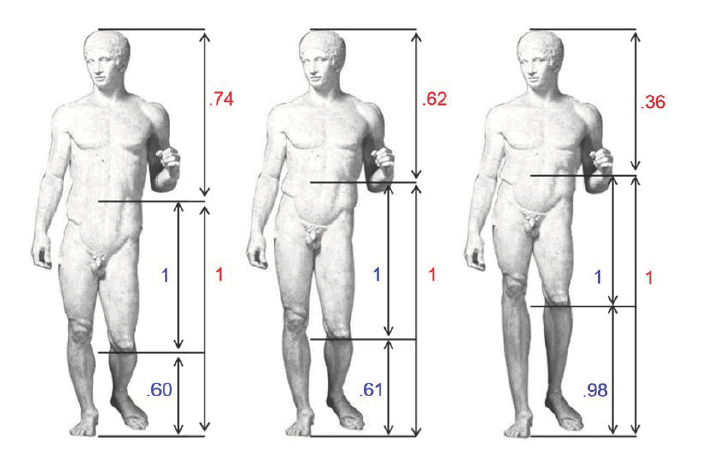
\includegraphics[width=3.80329in,height=2.4338in]{imgs/2.png}

Exemplo de estímulos canônicos e modificados. A imagem
original (\emph{Doryphoros}, de Polykleitos) é apresentada no centro da
figura. Essa escultura segue as proporções canônicas (proporção áurea =
1:1.618). Duas versões modificadas da mesma escultura são apresentadas à
esquerda e à direita. A imagem da esquerda foi modificada criando uma
relação de pernas curtas: tronco longo (proporção = 1:0.74), e a imagem
direita criando o padrão oposto de relação (proporção = 1:0.36). Todas
as imagens foram usadas em testes comportamentais. A imagem central
(considerada bonita em 100\%) e a imagem esquerda (considerada feia em
64\% foram utilizadas no estudo de \versal{IRM}f.}\footnote[20]{Figura extraída de Di Dio,
Macaluso e Rizzolatti (2007). Cortesia dra. C. Di Dio.}
\end{center}

Outros neuroesteticistas replicam que as deficiências de Jacobsen e seus
colegas se devem à afinidade desses autores com Kawabata e Zeki, e por
isso, se encontram longe demais do juízo estético ``per se''. Uma
tentativa de chegar mais perto, feita na Itália, estudou a ``reação
cerebral'' a imagens de esculturas clássicas e renascentistas
manipuladas para alterar a proporção áurea dos originais (Figura 2.2).

O objetivo do estudo era identificar se há ``uma base biológica objetiva
para a experiência da beleza'' ou se tal experiência é ``inteiramente
subjetiva'' (Di Dio, Macaluso e Rizzolatti, 2007, p.~1). A questão pode
ser traduzida para se ``parâmetros objetivos intrínsecos a obras de arte
são capazes de gerar um padrão neural específico subjacente à sensação
de beleza no observador'' (p.~6). Os autores tinham como hipótese uma
resposta positiva, a saber, que os humanos são dotados ``de mecanismos
específicos da espécie que ressoam em resposta a certos parâmetros
presentes em obras de arte'' (p.~6). A equipe alemã escolheu a simetria;
os italianos, a proporção áurea. Tanto simetria quanto proporção áurea,
há séculos, aparecem com destaque em pesquisas empíricas e filosóficas
sobre arte e experiência estética. O fato de que o debate sobre seu
papel e status ainda continue vivo sugere que essas caraterísticas não
representam questões meramente factuais, mas são densas condensações de
valores e visões de mundo. Mais pé no chão, nem os alemães nem os
italianos explicaram em que sentido os ``parâmetros objetivos'' que eles
alegavam investigar seriam ``intrínsecos'' às obras de arte, visto que
esses parâmetros estão ausentes em algumas obras de arte e presentes em
artefatos não artísticos, como na natureza.

A equipe italiana usou quinze conjuntos de três imagens, cada uma
incluindo quinze originais e quinze imagens modificadas (sete com
troncos longos e pernas curtas, oito com troncos curtos e pernas
longas); vinte esculturas representavam corpos masculinos, e dez, corpos
femininos. Os estímulos, trinta para cada uma das seis sessões distintas
de \versal{IRM}f, foram apresentados em ordem aleatória e durante dois segundos,
em três condições: \emph{observação}, na qual os sujeitos recebiam o
pedido de ``observar as esculturas como se estivessem em um museu'',
\emph{juízo estético} (os sujeitos foram perguntados se gostavam da
imagem), e \emph{juízo de proporção} (se consideravam a imagem
proporcional).

Foram realizados dois tipos de análises. Uma comparou ativações
cerebrais em reação a estímulos canônicos \emph{versus} modificados.
Essa análise deveria revelar ``as reações neurais a parâmetros objetivos
de beleza''. A hipótese era a de que a proporção áurea produziria
atividade aumentada em áreas que lidavam com o prazer e que o aumento de
sinal seria particularmente forte durante a condição de observação,
``quando a reação cerebral às obras de arte não tinha interferência de
pedidos cognitivos adicionais'' de julgamento (ibid., p.~2). (Pedir aos
sujeitos que olhassem para os estímulos \emph{como se estivessem em um
museu} obviamente não foi considerado um pedido significativo,
cognitivamente ou não.) Uma segunda análise, voltada para reações
cerebrais ``relacionadas com a apreciação subjetiva aberta dos
estímulos'', comparava ativações cerebrais obtidas durante as
apresentações de imagens consideradas bonitas e consideradas feias.

Os resultados comportamentais revelaram que imagens canônicas foram
avaliadas mais positivamente enquanto que as modificadas, mais
negativamente. Na análise de ressonância magnética, os resultados de ver
condições canônicas e modificadas foram primeiramente analisados em
conjunto, e, depois, comparados com o resto em todas as três condições
(observação, juízo estético e juízo de proporção). Essa comparação
revelou ``ativações'' em diversas áreas. Especialmente significativo
para os autores foi o aumento de sinal na ínsula durante a condição de
observação. A ínsula é uma das estruturas cerebrais mais estimadas pela
indústria do \emph{neuro}. Está relacionada com o controle motor e a
homeostasia, bem como com a interocepção e os estados viscerais
associados à experiência emocional, além de com o autoconhecimento e a
noção de ação. A insula parece desempenhar um papel tao crucial em
combinar informações sobre estados corporais em processos cognitivos e
emocionais de alto nível que, como disse um jornalista de divulgação
científica do \emph{New York Times}: ``O importante é que mente e corpo
são integrados na ínsula'' (Blakeslee, 2007).

Di Dio e seus colegas atribuíram um efeito de ativação mais fraco da
ínsula nas condições estética e de proporção ao pedido explícito de
julgar, que pode ter ``derivado os recursos de atenção dos voluntários
para um pedido cognitivo específico, desse modo reduzindo a reação
neural natural na ínsula'' (Di Dio, Macaluso e Rizzolatti, 2007, p.~4). A
partir desse fato parecia resultar que ``o \emph{sentimento} emocional
positivo produzido no observador pelas imagens canônicas foi determinado
por uma codificação preferencial dessas imagens, comparadas com as
modificadas, por diversas áreas corticais e por uma coincidente ativação
\emph{conjunta} da ínsula anterior'' (p.~6). Portanto, como a proporção
áurea ``determinou ativações cerebrais diferentes daquelas nas quais
esse parâmetro foi violado'', a questão sobre a existência de ``beleza
objetiva'' foi respondida positivamente (p.~6). Os autores reconhecem que
seria ``reducionista demais'' imaginar que a sensação de beleza ``ocorre
por causa'' da ativação da ínsula; é necessária a ativação conjunta de
muitas áreas e muitos circuitos. Em suma, as obras de arte poderão ``um
dia se tornar um patrimônio permanente da humanidade sem uma ressonância
induzida por alguns parâmetros biologicamente inerentes?'' (p.~8). A
resposta é obviamente ``não''.

Todavia, como qualquer catálogo dos atributos ou componentes essenciais
da humanidade (de variações do cânone ocidental à enumeração de traços
característicos da natureza humana), a lista desses parâmetros é
negociável, discutível e provavelmente reflete interesses particulares e
circunstâncias específicas. Ainda mais, o fato de que nossos cérebros
podem ser predispostos de um modo ou outro para determinadas qualidades
como proporção, simetria ou constância de escala não nos ajuda a
compreender melhor a experiência estética como \emph{experiência} e como
\emph{estética}. Mecanismos de percepção comuns certamente estão
envolvidos em olhar para a escultura de Andy Warhol \emph{Brillo Box} em
uma galeria e para as caixas originais de embalar Brillo de James Harvey
em um supermercado. O representante de Harvey se queixou como Warhol
usava o design do seu cliente, mas este admitiu, desanimado: ``O que é a
caixa de um homem pode ser a arte de outro homem'' (Gaddy, 2007). Embora
a neuroestética não queira analisar uma situação dessas, deveria pelo
menos ter os meios de levá"-la em conta. Tudo o que ela fez até agora, e
tudo o que pode fazer com sua metodologia e suas estruturas conceituais,
é correlacionar fatos conhecidos (reagimos emocionalmente a obras de
arte) ou algum aspecto limitadamente operacionalizado da relação
artística (especialmente apreciação) com a atividade de várias áreas do
cérebro, que estariam ``envolvidas'', ``associadas a'', seriam
``subjacentes'', ``contribuiriam com'' ou de um modo ou outro
``refletiriam'' esses fatos ou aspectos. Essas são ``as descobertas da
neuroimagem'' para compreender a ``experiência da arte'' (Nadal, 2013).

\section*{Empatia}
\addcontentsline{toc}{section}{Empatia \medskip}

Embora a beleza seja um tópico central na estética, a neuroestética da
beleza nos levou ao ponto de discorrer sobre se, a despeito do seu nome,
a nova disciplina trata realmente da estética. Com David Freedberg,
entramos em um mundo distinto --- um que promete um tratamento mais
sofisticado para a arte, bem como formas mais inteligentes de ligar
conhecimento neurocientífico e relação estética. De fato, Freedberg,
antes professor Pierre Matisse de História da Arte da Universidade de
Colúmbia, e desde 2015 diretor do Warburg Institute, tinha, antes de
voltar sua atenção para o cérebro, publicado amplamente sobre arte
holandesa, flamenga, francesa e italiana do século \versal{XVII} (incluindo
pintura, desenho e gravura), iconoclasmo, a interseção entre arte e
ciência e, em menor grau, arte contemporânea. O interesse de Freedberg
pelas neurociências diz respeito diretamente a acontecimentos históricos
que estudou em seu fundamental \emph{The} \emph{Power of Images}.

Nesse livro, Freedberg (1989) almejava, tal como Ernst Gombrich (1990)
observou em uma resenha afiada, ``levar a reação à arte de volta às
nossas reações elementares''. A passagem do autor para a neurociência
preenche esse desejo original e explica o poder das imagens com base nos
mecanismos neurobiológicos das reações empáticas automáticas. A
preocupação com a universalidade da reação e suas raízes psicobiológicas
transculturais levou Freedberg a considerar esse poder como uma
propriedade imanente e a \emph{procurar nas próprias imagens} o
princípio de sua eficácia, em vez de considerá"-las configurações que, de
modo a ter poder além de primitivos perceptuais, precisam envolver o
espectador e forças históricas e culturais (Prévolt, 2003). A devoção
cristã, por exemplo, pode ser inspirada não apenas pela representação
mais ou menos realista de cenas e personagens religiosos, mas também por
abstrações como retratos do Sagrado Coração ou do monograma de Cristo. O
sinal metafórico ou metonímico pode ter um poder cognitivo, afetivo e
existencial igual ao do objeto relacionado relevante, e é por isso que,
como diz Gombrich (1990), ``não há uma linha que alguém possa traçar
entre imagens, palavras ou sinais sagrados''. Em todos os casos é o
contexto que torna os objetos sagrados.

Como historiador do iconoclasmo, Freedberg (1985) sabe disso; como
neuroesteticista, entretanto, atribui a ``energia'' do Buddhapada, as
pegadas de pedra altamente reverenciadas que são antigas representações
não icônicas do Buda, à ativação de neurônios motores no sistema de
neurônios"-espelho do espectador (Freedberg, 2009c). Como as abstrações
cristãs já mencionadas, essas esculturas são objetos de devoção e
carregam poderes específicos em função de significados culturais (sejam
compreendidos no nível teológico mais elevado ou no da mera imitação
comportamental, com todas as nuances entre eles). Determinar se
neurônios motores são ativados quando olhamos para os traços do pé de
Buda não muda nada e (embora cientificamente interessante), não adiciona
ou subtrai coisa alguma de uma análise de seu poder: se os neurônios
motores de todos nós forem ativados ao contemplar as pegadas sagradas,
mas apenas alguns de nós sentirmos reverência religiosa (ou indiferença,
assombro estético, respeito histórico ou ódio fundamentalista), então
esses neurônios não desempenham papel fundamental em como experimentamos
Buddhapada. A posição de Freedberg reflete sua rejeição do ``modelo
padrão da ciência social'' que, em sua visão, impede a compreensão da
``relação entre a construção cultural de reações e esses aspectos da
reação que pertencem à nossa natureza humana'' (Freedberg, 2009c; ver
também 2007, 2008). A solução consiste em mudar o equilíbrio
investigativo e interpretativo para se concentrar em ``como a cultura
modula a biologia'' e em como ``a neurologia molda a história'' e
procurar ``invariáveis biológicas e psicológicas entre culturas''
(Freedberg, 2009c; 2007, p.~17 e 21).

Para Freedberg, assim como para outros, a virada neural irá renovar as
ciências humanas e torná"-las mais significativas. Na estética e na
história da arte, a neurologização dessas áreas irá conter ``visões
intelectualizantes da arte'' (Freedberg, 2009c) e permitir a
``eliminação do emocional, do empático e do âmbito da reaçao corpórea
não"-cognitiva'' que caracterizaria a maior parte da história da arte e
da crítica no século \versal{XX} (Freedberg e Gallese, 2007, p.~199). Nesses
campos, explica Freedberg (2007, p.~23), as emoções ``eram consideradas
demasiado aleatórias, constrangedoras e incidentais ao valor
transcendental da arte''. Enquanto a ``ortodoxia'' antropológica e da
história da arte supostamente se recusa a analisar reações emocionais
independentemente de seus contextos culturais e históricos, a pesquisa
neurocientífica, desde os anos 1990, corroborou noções de empatia como
sendo uma emoção corporificada que foi formulada inicialmente por
diversos filósofos, psicofisiologistas e historiadores da arte do final
do século \versal{XIX} e início do século \versal{XX} (Freedberg. 2007, p.~27-29; 2009a,
p.~87; 2009b, p.~70; Freedberg e Gallese, 2007, p.~198).

Freedberg não estaria erguendo um espantalho para fortalecer a sua
causa? Ele escolhe o filósofo norte"-americano Arthur Danto (1924-2013)
como um caso de visão ``intelectualizante'' segundo a qual reações
estéticas são ``puramente uma questão do modo pelo qual o conceito de
arte é considerado'' (Gallese e Freedberg, 2007). Porém, Danto nunca
propôs tal coisa. Na verdade, sua ideia era que distinguir obras de arte
de outras coisas, demandava que elas fossem consideradas ``artísticas''
em função de teorias, e, portanto, são essas teorias que tornam a
``arte'' possível (Danto, 1964). Afinal, não há evidências de que os
pintores de Lascaux ou seus contemporâneos acreditassem estar produzindo
arte. Ainda assim, hoje existe algo chamado arte pré"-histórica. Antes do
psiquiatra alemão Hans Prinzhorn e, entre outros, os artistas Paul Klee
e Vasili Kandinski no começo do século \versal{XX}, os desenhos, pinturas e
esculturas de doentes mentais, crianças e povos indígenas não se
consideravam como ``arte''. Durante o escândalo em torno à pintura
rupestre dos aborígenes australianos, um líder ngarinyin declarou:
``Algumas pessoas me disseram recentemente que a `arte da pedra está
morta'. Se a `arte' estivesse morta, isso não teria importância para nós
aborígenes. Nós nunca pensamos em nossas pinturas como `arte'. Para nós
elas são imagens'' (Mowaljarlai et al., 1988, p.~691). E essas imagens,
retratando os espíritos da nuvem e da chuva conhecidos como Wandjina,
precisam ser repintadas de modo a perpetuar a presença desses espíritos
e ``estimular as energias que trazem crescimento e renovação'' à
natureza (p.~692). A relação com as imagens é, em grande medida,
determinada por sua função e seu status.

A \emph{pop art} radicalizou tais conexões na criação da relação
estética. Danto descreveu seu desafio como sendo o de ``contrapartes
indiscerníveis que podem ter afiliações ontológicas radicalmente
distintas'', e perguntou: ``Por que \emph{Brillo Box} é arte quando as
caixas de Brillo no depósito são apenas embalagens de panos de limpeza
abrasivos?'' (Danto, 1981, p.~4; Danto, 1993). Pode haver, como o
filósofo reconhecia, um senso estético inato, mas as reações irão
diferir dependendo de como os objetos são classificados, e as diferenças
serão ``tão profundas quanto aquelas entre movimentos corporais e ações,
entre uma pessoa e um zumbi, entre uma divindade e um ídolo'' (Danto,
1981, p.~100). Em suma, se a reação estética às obras de arte envolve
processos que a reação a coisas não artísticas não envolve, então os
processos envolvidos em reagir à não"-arte não podem ser o que define a
arte ou a reação estética (ver também Danto, 1997, cap. 5). Tanto é
assim que a classificação prévia das obras de arte (como, por exemplo,
falsificações ou originais, Leder, 2001) realmente afeta as preferências
das pessoas. A neuroestética sustenta a suposição diametralmente oposta,
especificamente que a razão última para nossa reação a objetos está nas
propriedades dos objetos aos quais nossos cérebros reagem
automaticamente em função de sua fisiologia básica. Todo o resto é
complemento.

Para Freedberg, a chave deve ser encontrada nos neurônios"-espelho e nos
supostos substratos neurais da empatia e da corporificação. Juntamente
com Vittorio Gallese, o co"-descobridor dos neurônios"-espelho, elaborou
uma ``teoria das reações empáticas a obras de arte que não é puramente
introspectiva, intuitiva ou metafísica, tendo uma base material precisa
e definível no cérebro'' (Freedberg e Gallese, 2007, p.~199). Como isso
funcionaria?

Neurônios"-espelho constituem um sistema de células visomotoras que se
ativam não apenas quando um organismo realiza uma ação, mas também
quando observa uma ação similar realizada por outro organismo, da mesma
espécie ou não (Rizzolatti e Craighero, 2004; Gallese, 2009). Esse tipo
de neurônios foi descoberto no começo dos anos 1990 na área pré"-motora
F5 e posteriormente no lóbulo parietal inferior de macacos,
principalmente por inferência de estudos usando eletroencefalografia,
magnetoencefalografia e neuroimagem, e se acredita que também existiriam
em humanos (Gallese, 2007; 2008; revistos por Rizzolatti e
Fabbri"-Destro, 2010). Embora sua existência tenha sido questionada e
ainda persistam grandes dificuldades metodológicas, a conclusão mais
confiável até agora é de que ``mudanças no sinal \versal{BOLD} durante observação
da ação parecem consistentes com a existência de um sistema de
neurônios"-espelho em humanos, mas eles ainda não conseguiram fornecer
provas conclusivas'' (Kilner e Lemon, 2013, R1060; Caramazza et al.,
2014), e as discussões sobre neurônios"-espelho e seu funcionamento
prosseguem (por exemplo, em um fórum da publicação \emph{Brain and
Behavioral Sciences} sobre o artigo de Cook et al., 2014).

Quando descobertos, os neurônios"-espelho foram saudados como fornecendo
as bases da linguagem, da ``teoria da mente'' (a capacidade de atribuir
estados mentais a outros), da imitação, da empatia (e, consequentemente,
da moralidade), da arte, da cognição social, bem como da vida social e
da intersubjetividade em geral (daí a hipótese de que uma disfunção nos
neurônios"-espelho esteja na base do autismo). Grandes dúvidas foram
formuladas quanto às funções atribuídas aos neurônios"-espelho (p. ex.
Borg, 2007 em relação à atribuição intencional ou ``leitura da mente'';
Hickok, 2009 quanto à compreensão da ação; ou Jacob, 2008 em relação à
representação da intenção prévia de um agente; Rizzolatti e Sinigaglia,
2010 replicam que o circuito cerebral da observação"-execução da ação de
fato fornece ao indivíduo observador uma noção dos objetivos motores e
das intenções do outro indivíduo). De fato, a controvérsia --- que não
será resolvida apenas com evidências empíricas --- não acabou e, de
qualquer modo, não parece afetar às convicções dos neuroesteticistas.

Uma forma corrente de compreender o papel dos neurônios"-espelho é dizer
que \emph{simulam} (``espelham'') ações observadas, sejam realizadas ou
retratadas, e que tal ``simulação corporificada'' é a base para nossa
capacidade de compreender inconscientemente as ações, emoções e
sensações de outros. Por isso tal simulação pode funcionar como base
para uma abordagem da reação estética (Freedberg e Gallese, 2007). Olhar
para uma obra de arte produz nos espectadores (ou melhor, em seus
cérebros) a simulação da ação retratada ou corporificada na obra; a ação
pode ser a das figuras representadas, mas também o gesto motor criativo
do artista. Assim, o mármore ``\emph{Prisioneiros''} de Michelangelo
ativa nos espectadores as áreas cerebrais correspondentes aos músculos
que parecem ser exercitados na própria escultura. Quando contemplamos os
anjos cantores do altar de Gante de Hubert e Jan van Eyck, completado em
1432, ``é difícil'', alega Freedberg (2009b, p.~67), ``não querer
imitá"-los, até mesmo franzir o cenho com a aparente dificuldade de
cantar o que quer que estejam cantando''. A pesquisa estabelece que a
observação de movimentos bucais aumenta a excitação motora nas
respectivas áreas somatotópicas no cérebro, assim explicando as
capacidades de imitação de recém"-nascidos: tais descobertas, na visão de
Freedberg (2009b, p.~26-28) acrescentam ``contexto científico'' a
comentários muito mais antigos sobre o naturalismo vívido dos anjos dos
irmãos Eyck.

Nessa mesma linha, Freedberg afirma que, diante de um painel da
\emph{cantoria} de Luca della Robbia na catedral de Florença
(1421-1438), que mostra belos anjos cantores, ``o desejo de alguma forma
de emulação pode brotar no observador (\ldots{}) A arte de Luca é tão
impressionante que parece encorajar os espectadores, de um modo ou de
outro, a participar dos movimentos que o artista tão realisticamente
retrata'' (p.~72). O lirismo de Freedberg é eficaz, mas apela à sua
experiência e a um espectador universal genérico, em vez de a uma
demonstração empírica. \emph{A Incredulidade de São Tomé}, de
Caravaggio, no Sanssouci de Potsdam, mostrando o apóstolo colocando o
dedo na ferida do Cristo ressuscitado, leva a ``empatia por sensações
táteis'' (p. 201). E os \emph{Desastres da guerra} de Goya provocam
reações físicas nas mesmas partes do corpo que aparecem mutiladas nos
quadros -- uma empatia física que ``se transmuta facilmente em um
sentimento de empatia'' (Freedbeerg e Gallese, 2007, p.~197) e, assim,
abre caminho para uma reação moral. (Ver também Freedberg, 2008 sobre a
\emph{Dança dos camponeses} de Rubens.). Em conjunto com estudos da
mesma natureza, como o de Paul Ekman sobre as expressões faciais de
emoções, ou as de Peter Lang e outros sobre as reações afetivas,
faciais, viscerais e comportamentais de olhar para quadros, a pesquisa
de neurônios"-espelho parece adicionar substância empírica aos ensaios
clássicos de Elaine Scarry ou Susan Sontag sobre reações à dor dos
outros, e mesmo fornecer a base para uma ``narratologia corporificada''
(Gallese, 2011; Wojciehowski e Gallese, 2011).

Essas conjecturas não se aplicam apenas à arte figurativa. Contemplar as
\emph{action paintings} de Jackson Pollock ou as telas cortadas de Lucio
Fontana também provoca ``sentimentos empáticos corporificados'' em
resposta aos ``traços visíveis dos gestos criativos do artista, tais
como uma modelagem vigorosa em argila ou tinta, pinceladas rápidas e
sinais de movimentos da mão'' (Freedberg e Gallese, 2007, p.~199).
Freedberg e Gallese consideram os respingos e lágrimas dos artistas como
``traços visíveis de movimentos intencionais'' (p.~202). Mas uma máquina,
um chimpanzé ou um de nós poderia ter feito aquelas marcas
aleatoriamente, ou elas poderiam ser resultado do esforço calculado de
Mike Bidlo de criar um \emph{Not Pollock} que se parecesse exatamente
com o original. É uma questão empírica se nossos cérebros reagem da
mesma forma a imagens que parecem Pollock quando ``eles'' sabem ou não
sabem como as imagens foram feitas, ou se a simulação empática em frente
às telas talhadas de Fontana é verificável em sujeitos que carecem de
familiaridade com objetos afiados e superfícies esticadas.
Evidentemente, nossos sistemas de processamento visual podem reagir a um
Bidlo como a um Pollock, da mesma forma como podemos gostar ou desgostar
de certos objetos independentemente de serem classificados como
``arte''. Nossos cérebros provavelmente nos fazem sentir gestos que
aconteceram ou não. Mas percepção, consciência e experiência prévia com
o contexto (incluindo materiais, tamanho, posição, autoria e
categorização) contribuem decisivamente para o status dos traços que
supostamente geram a reação empática, e esse status, por sua vez,
desempenha um papel crucial em moldar nossa relação cognitiva e
emocional com eles.

Em experimentos usando diversos métodos (eletroencefalografia,
estimulação magnética transcraniana, rastreamento de olhos e mesmo
potencial evocado), Freedberg, Gallese e pesquisadores associados
chegaram a resultados que consideram um apoio empírico à tese da
``simulação corporificada'' (Battaglia, Lisanby e Freedberg, 2011;
Massaro et al., 2012; Sbriscia"-Fioretti et al., 2013; Umiltà et al.,
2012). Os pesquisadores mostraram, por exemplo, que ativação cortical
sensório"-motora durante a percepção de imagens estáticas de arte
abstrata ou efeitos de excitabilidade corticomotora ocorrem apenas
durante a observação de obras de arte originais (em oposição a uma cópia
ou fotografia mostrando um gesto que considerem ser o mesmo apresentado
no original). Como a maioria dos estudos em neuroestética, esses artigos
combinam metodologias altamente técnicas com surpreendentes fraquezas em
aspectos tão básicos quanto a escolha de estímulos e de situações de
controle. À parte disso, suas consequências para a estética são de dois
tipos.

Por um lado, esses experimentos, novamente como muitos na neuroestética,
pressupõem a possibilidade de critérios de base biológica para avaliar a
qualidade artística. A existência desses critérios foi evidente nas
investigações sobre beleza esboçadas acima, cujo objetivo, como tem sido
devidamente observado, é ``extrair regras que possam levar a uma
definição prática da beleza, conectando características de objetos e
atividade neural'' (Conway e Rehding, 2013, p.~1). Ainda que Freedberg,
Gallese e seus colaboradores não o digam, sugerem o mesmo objetivo
quando comentam sobre a correlação entre olhar para (a reprodução de) um
original e um efeito cerebral que interpretam como sendo evidência de
simulação corporificada: ``Como a observação da fotografia {[}de um
gesto{]} não afetou significativamente a excitabilidade corticomotora,
nós supomos que esse efeito, no caso da pintura {[}representando o
gesto{]} deve ser consequência da habilidade do artista em dar a
impressão ilusória de movimento'' (Battaglia, Lisanby e Freedberg, 2011,
p.~4). Tais observações criam as condições para uma aplicação dúbia de
inferência reversa: demonstre ativação cortical e você tem uma prova de
qualidade artística.

Por outro lado, precisamente por causa de sua concentração em processos
automáticos inconscientes ou pré"-conscientes, os experimentos que
acabamos de mencionar diferenciam entre \emph{experiência estética}, na
qual a simulação corporificada é ``um componente importante'', e
\emph{juízo estético}, que, corresponde à ``classificação estética
explícita de um objeto de acordo com cânones estéticos cultural e
socialmente determinados'', e representa ``o aspecto mais cognitivo da
relação estabelecida com obras de arte'' (Massaro et al., 2012, p.~15).
Na \emph{relação estética}, contudo, juízo e experiência (mesmo nos
sentidos simplificados dados aqui) são não apenas contínuos, como a
formulação citada sugere, mas constitucionalmente interdependentes.

A teoria da simulação corporificada baseada nos neurônios"-espelho,
então, nos leva de volta à questão: ``Em que a hermenêutica neural
contribui para a compreensão da arte e das relações estéticas e
artísticas?'' A interpretação com base cerebral propõe mecanismos que
possam ser universais, bem como necessários para compreender e reagir a
obras de arte. De fato, nós experimentamos sensações viscerais quando
encontramos corpos atormentados na arte. Mas também os sentimos diante
de prescrições para tortura judicial do início da modernidade ou
reportagens e fotografias jornalísticas contemporâneas de atrocidades ou
acidentes horrendos. Em todos os casos, podemos ser movidos por repulsa,
compaixão e indignação; podemos nos sentir estimulados a agir ou
paralisados de medo e desespero; podemos também ficar curiosos ou
admirar, considerar o objeto meritório ou desprezível, e podemos
experimentar qualquer combinação dessas emoções ou outras diferentes. Em
todos esses casos, o componente visceral"-espelho de nossas reações (a
suposta ``simulação corporificada'') pode ser concebido como primário e
automático, mas sua relevância termina no ponto em que questões de
estéticas mal começam. (A própria automaticidade também tem sido
questionada; Vignemont e Singer, 2006 sugerem que a empatia demanda uma
avaliação relacionada aos tipos de emoções envolvidas, a relação entre
aquele que demostra empatia e alvo, as características daquele que
demostra empatia e o contexto situacional.)

Estudos do ``cérebro empático'' (Keysers, 2011) identificaram regiões
``envolvidas'' na capacidade humana de compreender as sensações,
intenções e emoções de outras pessoas. Contudo, a atividade dessas
regiões pode não ser mais do que uma condição da relação estética, e
aquilo com que a pesquisa contribui não é nada além ``de uma história
adicional da `implementação' acerca de nossas reconhecidas capacidades
de reagir a representações visuais'' (Davies, 2014, p.~11). No fundo, a
questão é se a atividade dos neurônios"-espelho e neurônios ``canônicos''
é constitutiva da reação estética\footnote[21]{Neurônios canônicos, também na área F5 do córtex pré"-motor ventral
de macacos, disparam quando vemos um objeto que pode ser segurado pelo
movimento preênsil da mão cujos movimentos esses neurônios codificam.}. Respondendo à
David Freedberg e Vittorio Gallese, dois cientistas cognitivos e
filósofos da percepção argumentaram que a proposta dos autores de uma
base neural para reações empáticas à arte estava ``aberta à acusação de
irrelevância em relação às questões da experiência estética e o do que
constitui a obra de arte'' (Casati e Pignocchi, 2007). Os autores
enfatizaram que o testemunho de cenas reais que correspondem a
representações artísticas produz reações neurais ``relevantemente
similares'', então a ativação neuronal ``não é suficiente para a
avaliação estética ou para julgar se algo é uma obra de arte''. Gallese
e Freedberg (2007) responderam que ``neurônios"-espelho e neurônios
canônicos são elementos cruciais na reação estética''. Para eles, a
avaliação estética demanda a corporificação simulada e o envolvimento
empático que se segue à observação visual por intermédio de atividade de
neurônios"-espelho; tais processos ``podem ser pré"-cognitivos'' e ``nem
sempre'' moldados por cognição e cultura. Ademais, na medida em que a
``habilidade artística'' reside na capacidade dos artistas produzirem
reações emocionais e sensações motoras nos espectadores, a visão
``intelectualizante'' (como a de Danto) da reação estética precisa estar
errada.

Os dois lados parecem nem mesmo entender ``constitutiva'' e ``crucial''
da mesma forma. Ainda assim é revelador que neuroesteticistas sublinhem
que as reações que estudam se aplicam ``no caso de imagens menos
conhecidas --- e algumas vezes cotidianas'' (Gallese e Freedberg, 2007).
De fato, fazer com que essas reações, e seus mecanismos, desempenhem
\emph{o} papel essencial na reflexão sobre a arte implica que as
diferenças, perceptuais ou outras, entre um Mondrian, o Partenon e uma
grade (ou uma pintura e sua reprodução, uma foto de passaporte e \emph{A
Verônica} -- o pano em que o rosto de Cristo foi supostamente impresso)
são irrelevantes para compreender a reação estética. Não apenas a
neuroestética negligencia a materialidade, e com ela tamanho, textura,
cor e escala; também não diferencia o retrato de um martelo e o martelo
real que alguém pode agarrar, a pessoa retratada e a pessoa real com a
qual alguém interage. A disciplina despreza a diferença radical entre as
``\emph{affordances}'', as distintas possibilidades de ação oferecidas
pelas coisas e por suas imagens.

Perceber uma obra de arte pode preparar neurobiologicamente o espectador
para ações ou interações, mas elas não serão necessariamente realizadas.
Dessa forma, a arte transcende as possibilidades reais de ação
relacionadas ao que representa ou transmite, mas, da mesma forma, abre
novas possibilidades diferentes (Gallagher, 2010). Não há necessidade de
negar a existência de processos primitivos perceptuais ou automáticos
crescentes ``\emph{bottom"-up}'' para compreender que a neuroestética
despreza distinções que são essencialmente relevantes para a teoria, a
prática, a história e a recepção da arte, e em geral para a relação
estética. Concordamos com o filósofo David Davies (2014, p.~12) em que
evidências empíricas do tipo fornecido pela nova disciplina podem
``informar'' a estética, mas que a ``maioria das questões filosóficas
significativas não pode ser resolvida apelando a esse trabalho''. Para a
neuroestética, uma objeção como essa não é sequer compreensível, já que
todo o seu projeto supõe que a estética foi fundamentalmente equivocada
até que se começasse a levar em conta o cérebro.

Em suma, a experiência estética começa onde a neuroestética termina; ou,
como definiu o filósofo Alva Noë (2015, p.~361), na neuroestética ``a
arte não é explicada; ela é descartada''. De fato, a neuroestética
demanda que desistamos do próprio conceito de ``arte''. Isto é, que o
empobreçamos ao ponto de considerar seus produtos uma forma primitiva de
imagens do cérebro e a beleza como o resultado automático da disposição
de estímulos visuais (Cappelletto, 2009, p.~151- 152). De forma mais
genérica, a disciplina transfere a arte para uma estrutura epistêmica
que exclui a noção de obras intencionalmente produzidas (Fimiani, 2009).
Talvez tenha sido essa a direção à qual Freedberg apontou em \emph{The
Power of Images} quando se lamentou de que nossa percepção é nublada
pela ``compulsão de definir se um objeto é arte ou não''. Há, de fato,
ocasiões em que essa compulsão e o discurso que a cerca são obstáculos
para sentir e compreender. Porém, para a \emph{arte} continuar a ser uma
noção significativa, e a \emph{relação estética} uma experiência
significativa, apenas córtex sem contexto não bastará.

\chapter{3. Cerebralizando o sofrimento psíquico}

A partir da exploração das neurodisciplinas que lidam com cultura e
produções culturais concluímos que ``córtex sem contexto não bastará''.
Com isso queríamos resumir a observação de que as metodologias que
demandam deixar de fora ou que são incapazes de levar em conta fatores
contextuais acabam negligenciando os objetos e processos que alegam
estar estudando --- objetos e processos que são intrinsecamente
contextuais. Mas se há uma área em que o papel do contexto tem sido o
cerne do debate é a compreensão e administração do sofrimento mental em
todas as suas formas. (Vamos manter o termo ``sofrimento'', embora, como
veremos depois, em relação à neurodiversidade, nem todas as pessoas
diagnosticadas concordam em que sofram ou que seu sofrimento possa ser
atribuído ao quadro diagnosticado.) Contextos controversos aqui incluem
toda a gama do genético ao biográfico, do familiar ao étnico, econômico
e sociopolítico. Embora o papel desses ambientes no sofrimento mental
seja amplamente reconhecido, a discussão é sobre seu peso relativo e em
como melhor compreender suas interações. A ``cerebralização'' do
sofrimento psicológico há muito tem estado no cerne dessa discussão.
Embora divergências frequentemente tenham envolvido dicotomias claras
entre natureza e cultura, ou visões reducionistas de diferentes tipos
(pois a redução pode ser tanto cultural quanto genética ou
neurobiológica), escolhemos neste capítulo enfatizar os modos
ambivalentes pelos quais o \emph{neuro} serve a uma variedade de
alegações e objetivos com frequência opostos.

\section{Os mecanismos da cerebralização}

Em um artigo publicado na \emph{Nature} em 2008, Steven Hyman, um
professor de neurobiologia de Harvard e diretor do Instituto Nacional de
Saúde Mental norte"-americano de 1996 a 2001, reconheceu que ``a despeito
da carga de doença atribuível a transtornos neuropsiquiátricos, e a
despeito de pesquisas significativas, seus mecanismos de patogênese e
fatores de risco genéticos e não genéticos continuam teimosamente fora
do alcance'' (Hyman, 2008, p.~890). Imediatamente após sua avaliação
bastante sombria, Hyman alegou que esse ``alarmante estado de coisas
está começando finalmente a melhorar, em parte graças à aplicação de
novas tecnologias genéticas associadas a avanços na neurociência''. Esse
``facho de luz'' anunciava um ``novo alvorecer'' no diagnóstico e
tratamento de ``transtornos neuropsiquiátricos'' (p.~893). Poderíamos
citar dezenas de declarações marcadas pela mesma estrutura:
primeiramente uma observação fortemente pessimista sobre a situação
``atual'', depois uma afirmação de esperança em descobertas futuras na
compreensão da patogênese. Essas descobertas dependem da crença
subjacente em que o sofrimento psicológico é essencialmente um estado do
cérebro e precisa ser fundamentalmente compreendido e explicado como
tal, uma crença também expressa no uso habitual de \emph{transtorno
cerebral} e \emph{neuropsiquiatria} para se referir ao que costumava ser
chamado de \emph{transtorno mental} e \emph{psiquiatria}.

Hyman define ``transtornos mentais'' como um ``grupo amplo de
transtornos cerebrais'', afetando principalmente ``emoção, cognição
superior e função executiva''. De fato, para ele a expressão
``transtornos mentais'' é um ``anacronismo infeliz'' remontando a uma
época em que as condições assim chamadas ``não eram universalmente
entendidas como refletindo anormalidades na estrutura do cérebro, sua
conectividade ou função''. Assim disseminada, tal convicção é, como
acabou de ser mencionado, invariavelmente acompanhada pelo
reconhecimento igualmente geral de que identificar anormalidades neurais
precisas subjacentes a esses transtornos tem ``teimosamente desafiado''
os esforços de pesquisa (Hyman, 2007, p.~725). Pelo menos desde os anos
1990 essa dubiedade tem sido uma caracterização central da
cerebralização do sofrimento psíquico e, portanto, também de como esse
processo tem afetado à identidade pessoal e à autocompreensão.

Existe hoje um grande volume de trabalhos antropológicos e sociológicos
sobre essas questões. Parte dele lida com como a neuroimagem, sendo um
grande vetor da cerebralização, contribuiu para moldar subjetividades e
tem sido incorporada aos discursos e práticas não apenas de pacientes,
mas também de grupos de pais e profissionais de saúde (p. ex., Borgelt et
al., 2012; Buchman et al., 2013; Cohn, 2010, 2012; Dumit, 2003, 2004;
Eijkholt, Andersson e Illes, 2012; Illes et al., 2008). Em seu estudo
etnográfico pioneiro da exploração da mania e da depressão na cultura
norte"-americana, a antropóloga Emily Martin examinou a disseminação do
vocabulário de base cerebral na psiquiatria e seu impacto em questões de
identidade pessoal e autoidentificação (Martin, 2007, 2010). O caso do
alcoolismo (e poderíamos mencionar outros) ilustra como a tendência a
mapear a pessoalidade e as doenças no cérebro por intermédio de uma
``neurologia popular'' pode coexistir com e preservar, em vez de abalar,
antigas ideias (Vrecko, 2006).

Os processos de subjetivação em operação na área dos transtornos mentais
exemplificam um fenômeno que observamos ao discutir a questão do
\emph{sujeito cerebral} no Capítulo 1: ideias neurocientíficas não
necessariamente transformam autocompreensões de modo radical, mas se
combinam com percepções existentes e às vezes reforçam normas vigentes.
Assim, a adição compreendida como um transtorno cerebral acaba
reforçando, em vez de enfraquecendo, o apelo à responsabilidade
individual. Manter um cérebro saudável implica ``um modo de vida
caracterizado por uma cidadania autônoma e responsável'', e para
atingi"-lo a força de vontade exercida de maneira ativa é mais importante
que tomar passivamente uma medicação (Netherland, 2011, p.~172).

Resumindo, a cerebralização do sofrimento psicológico não é algo
simples, e a ambivalência é uma de suas características centrais. No
plano da experiência individual e grupal, interpretar a doença mental
como um quadro cerebral pode ser liberador, mas também pode gerar novos
estereótipos e mecanismos de exclusão; pode inspirar novas socialidades,
mas também erguer barreiras identitárias. No plano científico, a
cerebralizão do sofrimento psíquico promete ser a fonte de avanços em
diagnóstico e tratamento, mas mesmos seus protagonistas reconhecem meio
século de poucos avanços e muitos fracassos. Neste capítulo, iremos
estudar essas dinâmicas por intermédio de dois casos, um concentrado na
pesquisa científica, e o outro na construção de subjetividades coletivas
e individuais: a neuroimagem da depressão e a afirmação do autismo como
uma forma de ``neurodiversidade''. Antes disso, porém, precisamos
esboçar alguns elementos importantes dos contextos mais amplos aos quais
ambos pertencem, qual sejam a emergência do ``nexo farma"-psique'', a
globalização da saúde mental, a lógica dos biomarcadores e a crise do
modelo biológico.

\section{Farma"-psique}

A expressão \emph{nexo farma"-psique (pharma"-psyc nexus)} (Williams, Katz
e Martin, 2011) tem sido usada para dar ideia da disseminação de
produtos psicofarmacêuticos que lidam com a química cerebral. Isso
inclui, entre outros, a comercialização de inibidores seletivos de
recaptação de serotonina (\versal{SSRI}s, na sigla em inglês) para depressão e
transtornos relacionados à ansiedade, e de psicoestimulantes como
metilfenidato (bem conhecido pelo nome comercial Ritalina) para \versal{TDAH},
bem como o uso dessas e de outras substâncias como modafinil (indicado
para o tratamento de narcolepsia) com objetivos recreativos e de
aprimoramento. Em seus livros \emph{The Antidepressant Era} (1997),
\emph{The Creation of Psychopharmacology} (2002), \emph{Let Them Eat
Prozac} (2004), \emph{Mania: A Short History of Bipolar Disorder} (2008)
e \emph{Pharmaggedon} (2013) o psiquiatra e historiador David Healy
estudou criticamente o conluio entre a medicina e a industria
farmacêutica, particularmente no campo da saúde mental, tendo a
depressão como caso principal (ver também Bentall, 2009; Greenberg,
2010; Kirsch, 2009). Healy e outros demonstraram em que grau a produção
de evidências na psiquiatria foi cooptada por interesses econômicos e
comerciais. Laboratórios farmacêuticos se valem de práticas de
\emph{ghost"-writing} tendenciosas, garantem que apenas resultados
positivos sejam publicados, ao mesmo tempo reformulando ou escondendo
resultados negativos de testes clínicos, e exageram a eficácia de
medicamentos (Angel, 2004; Dumit, 2012; Goldacre, 2013; Gupta, 2014;
Healy, 2004, 2008; Kirmayer e Raikhel, 2009). Como a abordagem
farmacológica alimentou a expansão da doença até as atuais proporções
epidêmicas, o sistema se sustenta (Whitaker, 2010).

O esforço da farma"-psique não é apenas uma questão de economia e
medicina, mas também de ética profissional. O financiamento pela
indústria farmacêutica de pesquisas e formação biomédicas gera conflitos
de interesse que médicos e pesquisadores com frequência preferem não
revelar. Empresas usam incentivos materiais para aumentar o volume de
receitas e estimulam a adoção de novas drogas em prejuízo de genéricos
disponíveis; a maioria dos médicos americanos aceita presentes, mas
tende a minimizar a influência deles (Armstrong, 2012; Gibbons et al.,
1998; Grande, 2010; Green et al., 2012; Grande, Shea e Mitchell, 2009;
Hodges, 1995; Wazana, 2000). Essa situação levou a uma diminuição
significativa da confiança pública e a intensas discussões sobre como
melhor regulamentar esse setor da profissão médica (Grande, 2010).

Como pode ser visto em centenas de fóruns na internet, a confiança
também foi abalada por outros fatores. Um é a consciência crescente de
que a disseminação do uso de medicamentos específicos expande as
fronteiras do diagnóstico e até mesmo gera novas categorias
diagnósticas. A depressão, por exemplo, foi ampliada para incorporar
pesar, tristeza e timidez --- estados que, mesmo quando intensos ou
prolongados, não necessariamente indicam doença mental (Frances, 2013;
Horwitz e Wakefield, 2007; Lane, 2007). Outro fator diz respeito aos
medicamentos. A descoberta, nos anos 1950, do efeito antipsicótico e
antidepressivo de certos compostos sintéticos (clorpromazina foi o
primeiro) e a posterior introdução da prescrição de drogas psicotrópicas
levou à alegação de que a doença mental é causada por um ``desequilíbrio
químico'' no cérebro (Whitaker, 2010). No que diz respeito à depressão,
a tese do ``desequilíbrio'' foi sustentada pelo fato de que os \versal{SSRI} têm
efeitos antidepressivos em alguns pacientes. Na verdade, nem a causa
desses efeitos, nem as formas de ação dessas drogas são conhecidas.
Muitos chamam a teoria do desequilíbrio de um ``mito'', e é claro que
deve ser visto no mínimo como uma metáfora (Moncrieff, 2008). Mas essa
teoria tem sido reproduzida acriticamente pelos meios de comunicação e
defendida com um sucesso por psiquiatras e pela indústria farmacêutica,
para os quais tem tido um enorme valor de marketing (Lacasse e Leo,
2005; Leo e Lacasse, 2008).

Ao contrário do que afirma a publicidade farmacêutica sobre a ação de
medicamentos específicos, as drogas psiquiátricas carecem de
especificidade e têm efeitos cumulativos que não correspondem
perfeitamente a sintomas, transtornos ou neurotransmissores específicos.
Os laboratórios farmacêuticos, porém, sorrateira e intencionalmente
cometeram a ``falácia terapêutica'' de sugerir que as drogas que
anunciam são sustentadas por uma teoria causal sobre a psicopatologia
visada. A teoria, contudo, parece válida principalmente porque a droga
comercializada melhora certos sintomas. Debates recentes sobre
antidepressivos testam três possíveis explicações para a eficácia desses
medicamentos: são eficazes porque seu componente ativo tem uma ação
psicodinâmica específica e dirigida (essa é a razão comercialmente mais
interessante); o efeito placebo é responsável pela eficácia do
medicamento; ou as drogas têm algum mecanismo de ação desconhecido que
provoca um estado mental alterado não específico juntamente com um
efeito placebo (Gupta, 2014, p.~59).

A psiquiatra e bioeticista Mona Gupta observa que ``as três
interpretações são plausíveis, mas nenhuma é obviamente verdadeira ou
falsa'' (p.~59). Agora, se esse é o caso, então a comunidade psiquiátrica
tem a prerrogativa de determinar qual é mais provável. Interesses
profissionais e financeiros tendem a fazer a escolha pender para a
primeira explicação, que pressupõe eficácia antidepressiva específica.
Donde, como Edward Shorter (2013, p.~4-5) coloca de forma penetrante,

\begin{quote}
Hoje, com a disseminação dos diagnósticos de depressão, temos a ideia de
que desânimo e incapacidade de experimentar o prazer são nossos
principais problemas; nos vemos como tendo um transtorno de humor
localizado unicamente no cérebro e na mente, que antidepressivos podem
corrigir. Mas isso não é ciência; é publicidade farmacêutica.
\end{quote}

\section{Globalização}

O marketing psicofarmacêutico também contribuiu para a globalização da
psiquiatria e a alta prevalência de depressão, como documentado por
pesquisas em Índia, (Ecks, 2013; Ecks e Basu, 2009; Sumeet e Jadhav,
2009), Japão (Appelbaum, 2006; Kirmayer, 2002; Kitanaka, 2011), Brasil
(Béhague, 2009; Biehl, 2005, 2006; Leibing, 2009) e Argentina (Lakoff,
2005, 2006). Embora estudos etnográficos tendam a corroborar a
existência de uma hegemonia psicofarmacêutica global (Good, 2010), a
distribuição de gastos em produtos farmacêuticos é fortemente
assimétrica e determinada por incentivos econômicos (Petryna e Kleinman,
2006). Na área de saúde mental, o resultado é excesso de diagnósticos e
medicação nos países mais riscos e desastrosa negligência nos mais
pobres (Kleinman, 2012).

Tal desequilíbrio na distribuição dos recursos deve ser vista no quadro
da discussão sobre a contribuição dos transtornos mentais para a carga
global das doenças (Global Burden of Disease - \versal{GBD}, na sigla em inglês),
medida na esperança de vida corrigida pela incapacidade
(disability"-adjusted life years - \versal{DALYS}, na sigla em inglês, ou número
de anos perdidos em função de problemas de saúde, incapacidade ou morte
precoce). Quadros neuropsiquiátricos, incluindo casos comuns como
depressão e ansiedade, transtornos de adição (álcool e substâncias
controladas) psicoses e demência são responsáveis por até um quarto de
todos os \versal{DALY}s e até um terço daqueles atribuídos a doenças
não"-transmissíveis, com alta variação por países e níveis de rendimento
(Prince et al., 2007, 2014). A depressão é considerada a maior
responsável pelo \versal{GBD} e, juntamente com o transtorno de ansiedade,
reponde por entre um quarto e um terço de todas as consultas médicas ao
redor do mundo (Prince et al., 2014, p.~103). A grande carga imposta
pelos transtornos mentais, segundo estimativas epidemiológicas, coexiste
com a posição secundária da saúde mental naa agenda e nas políticas de
saúde global. O movimento de Saúde Mental Global (\emph{Global Mental
Health} -- \versal{GMH}, na sigla em inglês), que foi lançado pelo jornal médico
britânico \emph{The Lancet} em 2007, destaca a ``lacuna de tratamento''
entre a necessidade e a disponibilidade de serviços de saúde mental,
especialmente em países de renda baixa e media. Para superar essa lacuna
a Organização Mundial de Saúde (\versal{OMS}) criou em 2008 o ``Mental Health Gap
Action Programme'' (mh\versal{GAP}) (Cohen, Patel e Minas, 2014; Hanlon, Fekadu e
Patel, 2014; Patel, 2012; \versal{OMS}, 2008).

Essas propostas foram acompanhadas de polêmica, por exemplo, quanto à
validade de instrumentos de diagnóstico em diferentes países e a
confiabilidade de estimativas epidemiológicas sobre a prevalência global
dos transtornos mentais (Mills, 2014; Summerfield, 2008, 2012; Watters,
2010). Contudo, divergências quanto a aspectos técnicos dizem respeito
ao quadro conceitual que funde transtorno mental com transtorno
neurológico, a suposição fundamental de que doenças mentais são
essencialmente transtornos cerebrais. É inerente na localização cerebral
do transtorno mental a hierarquia epistemológica que destacamos no
capítulo anterior: acredita"-se que apenas a descoberta de causas
neurobiológicas satisfará a ambição de ``definir a verdadeira loucura''
e que assim a ``real'' contribuição do transtorno mental para o \versal{GBD} será
estabelecida (Rose e Abi"-Rached, 2013, p.~130).

Tais convicções sobre causalidade (ao que retornaremos) são relevantes
para a luta, presente no movimento \versal{GMH}, para reconciliar universalidade
biológica e particularidade cultural. Diferentes culturas têm diferentes
crenças sobre o significado da \emph{mente} e das relações mente"-corpo,
mas é aceito que os cérebros são basicamente iguais na espécie humana. O
Relatório Mundial de Saúde de 2001 afirma: ``Transtornos mentais não são
exclusividade de qualquer grupo social; eles são verdadeiramente
universais. Transtornos mentais e comportamentais são encontrados em
pessoas de todas as regiões, todos os países e todas as sociedades''
(\versal{OMS}, 2001, p.~23). A universalidade da doença é neste caso sustentada
por uma neurobiologia universal, que justifica introduzir em diferentes
contextos culturais pacotes de intervenção e modos de diagnóstico
transculturais e ao mesmo tempo reconhecer variação no nível da
expressão e dos deflagradores da psicopatologia (Cohen, Patel e Minas,
2014; Patel, 2012; \versal{OMS}, 2013).

Contudo, desde meados dos anos 1990, e pelo menos no movimento \versal{GMH}, a
universalidade da doença se dissociou da globalização da nosologia e
mesmo da utilização global da própria noção de ``transtorno mental''.
Profissionais de atenção primaria em países em desenvolvimento estão
desconfortáveis com essa noção e ``argumentam que a utilização de
sintomas para diagnosticar transtornos mentais, sem levar em
consideração o contexto (\ldots{}) essencialmente indica sofrimento não
significativo clinicamente'' (Jacob e Patel, 2014, p.~1433). Assim,
notando, por exemplo, que em países de renda baixa ou media ``muito
poucos pacientes dizem sentir depressão'', e que a maioria das
intervenções para a depressão evita aplicar o rótulo, dois importantes
membros do \versal{GMH} defenderam não apenas abordagens dimensionais para o
sofrimento, mas o abandono das atuais classificações internacionais em
prol de uma nova taxonomia de baixo para cima que seria elaborada
independentemente dos pontos de vista de especialistas (Jacob e Patel,
2014; comparar com Patel e Winston, 1994).

\section{Biomarcadores}

No nível da pesquisa a suposição de que o sofrimento mental envolve
anomalias no cérebro alimenta a busca de biomarcadores que possam
distinguir de uma manira más eficaz normalidade e patologia, captar
fatores etiológicos e ajudar no desenvolvimento de tratamentos que sejam
efectivos por visar as anormalidades pretendidas. Mas mesmo os mais
ferrenhos defensores da abordagem neurobiológica reconhecem que os
biomarcadores permanecem ``teimosamente fora de alcance'' (Hyman, 2008,
p.~890). Em 2002, em uma contribuição para a preparação da quinta edição
do \versal{DSM}, o \emph{Diagnostic and Statistical Manual of Mental Disorders}
da Associação Psiquiátrica Americana (lançado em 2013), um grupo de
destacados psiquiatras biológicos observou que a psiquiatria havia ``até
então fracassado em identificar um único marcador fenotípico
neurobiológico ou gene que seja útil para fazer um diagnóstico de um
transtorno psiquiátrico importante ou prever a reação ao tratamento
psicofarmacológico'' (Charney et al., 2012, p.~33). Mais de década e meia
depois a situação não mudou.

Assim, um artigo de 2011 sobre os desafios envolvidos na busca de
marcadores biológicos para o autismo concluiu que ``a despeito de
enormes avanços na compreensão científica básica do autismo,
comparativamente pouco foi conseguido até agora em relação a traduzir as
evidências resultantes em biomarcadores clinicamente úteis'' (Walsh et
al., 2011, p.~609-610). E em 2014 a neuropsiquiatra da Emory University
Helen S. Mayberg, figura de destaque no campo da neuroimagem da
depressão, admitiu, pessimista, que ``as afirmações dos clínicos de
poder usar o escaneamento estrutural ou funcional do cérebro com
confiabilidade'' com objetivo de diagnóstico e tratamento ``carecem de
apoio clínico ou científico''. Ainda pior, tais afirmações estão ``além
do alcance da pesquisa atual e dão falsas esperanças aos pacientes e a
suas famílias'' (Mayberg, 2014, S34).

A razão para tais fracassos reside, pelo menos em parte, nas categorias
para as quais os biomarcadores estão sendo buscados, que são aquelas
fornecidas pelo \emph{\versal{DSM}} e a \emph{\versal{CID}} (a \emph{Classificação
Internacional de Doenças} da \versal{OMS})\footnote[1]{O \versal{DSM} está agora em sua quinta edição (\emph{\versal{DSM}"-5} 2013,
\textless{}\emph{http://www.dsm5.org}\textgreater{}); o \emph{\versal{CID}} está na undécima edição
(\emph{\versal{CID}"-11}, \textless{}\emph{https://bit.ly/2UbWXWk}\textgreater{}),
lançada em junho de 2018.}. Possivelmente não
há biomarcadores para os agrupamentos de sintomas que essas
classificações identificam como categorias diagnósticas. Daí a
iniciativa do Instituto Nacional de Saúde Mental americano (\versal{NIMH}),
lançada em 2011, de abandonar as categorias do \versal{DSM} e desenvolver
``Critérios de Domínio de Pesquisa'' (\emph{Research Domain Criteria} -
\versal{RD}o\versal{C}, na sigla em inglês) com o objetivo de transformar o diagnóstico
psiquiátrico por intermédio da convergência de genética, neuroimagem e
ciência cognitiva (Insel et al., 2010; Insel, 2013; Kapur, Phillips e
Insel, 2012).

\versal{RD}o\versal{C} representa um novo ângulo na busca de marcadores neurobiológicos,
mas não um novo ponto de partida radical. Na verdade, eles mantêm
intacta a visão neurobiológica estabelecida do transtorno mental, com
sua atenção em mecanismos biológicos definidos às custas de uma
abordagem ``ecossocial'' mais integrada (Kirmayer e Chafa, 2014). Pelo
\versal{RD}o\versal{C} os biomarcadores não serão mais associados a categorias do
\emph{\versal{DSM}}, mas as doenças mentais continuarão a ser definidas como
``transtornos biológicos envolvendo circuitos cerebrais que implicam
domínios específicos de cognição, emoção ou comportamento'' (Insel,
2013). O problema é que elucidar a etiologia desses transtornos demanda
``confiança no cérebro, não no \versal{DSM}'' (Rose, 2013b, p.~10), mas confiar no
cérebro até agora praticamente não produziu nenhum resultado de uso
clínico ou diagnóstico. Os achados de neuroimagem teriam supostamente
correlação com aprendizado e desempenho em crianças e adultos,
criminalidade, comportamentos relativos à saúde e respostas a
tratamentos, e foi alegado que na medida em que possam funcionar como
neuromarcadores, podem contribuir para personalizar práticas nesses
campos (Gabrieli, Ghosh e Whitfield"-Gabrieli, 2015). Mas a situação
permanece como Nikolas Rose e Joelle Abi"-Rached (2013, p.~138) a
descreveram, isto é, ``Cada uma das trilhas que a neuropsiquiatria
tentou traçar pelo cérebro parece levar não aos planaltos brilhantes da
clareza, mas à escura, úmida, enevoada e misteriosa floresta da
incerteza''. Talvez o motivo seja que o \versal{RD}o\versal{C} se baseie no modelo de
doença cerebral da saúde mental justo em um momento em que o modelo
``bio"-bio"-bio'' (Read, 2005; Read, Bentall e Fosse, 2009), que combina
neurobiologia, genética e farmacologia, se encontra sob ataque nos
níveis epistemológico, ontológico, sócio"-moral e cultural.

\section{Crise do modelo ``bio"-bio"-bio''?}

Quais são as bases para as críticas ao modelo ``bio"-bio"-bio''?
Primeiramente, medicamentos recentes e a princípio mais eficientes não
funcionaram como se antecipava. A nova geração de antipsicóticos não é
mais eficaz que drogas mais antigas e (agora) muito mais baratas, como
Amplictil, uma marca de clorpromazina. Ademais, as novas drogas foram
relacionadas a morte cardíaca repentina, risco cardiovascular, ganho de
peso e desenvolvimento de diabetes (Álvarez"-Jiménez et al., 2008; Foley
e Morley, 2011; Luhrmann, 2012; Ray et al., 2009; Weinmann, Read e
Aderhold, 2009). O desencanto farmacológico corresponde ao fracasso em
identificar biomarcadores genéticos e neurobiológicos, e é reforçado por
evidências do papel da cultura na prevalência e prognóstico de
transtornos como esquizofrenia (Luhrmann, 2007, 2012; mas como Cohen e
Gureje {[}2007{]} documentam, produzir e assimilar evidências sobre
essas questões de formas que não sejam fortemente determinadas por
interesses e pontos de vista preconcebidos é tão difícil em relação à
cultura quanto em relação à biologia).

Em segundo lugar, as terapias psicológicas estão de volta. A
cerebralização da psiquiatria entrou em conflito com abordagens
psicodinâmicas, principalmente psicanalíticas, sobre questões de
eficácia, validade diagnóstica e prevalência. Os atuais debates sobre
\versal{GMH} e a articulação de universalidade e particularidade nos transtornos
mentais constituem o capítulo mais recente da atual tensão, que parece
entrar em uma nova fase. De fato, como veremos a seguir, a retirada
recente de classificações contemporâneas prevalentes está na base de uma
mudança para a completa ``desnosologização'' da doença mental, ou seja,
abrir mão de categorias diagnósticas como as conhecemos, para se
concentrar em dimensões que podem ser diversamente combinadas e tratadas
de modos sensíveis ao contexto no nível comportamental e psicológico.

Considerando a evidência de que a eficácia dos antipsicóticos foi
superestimada --- e sua toxidade subestimada~---, bem como dados que
surgem sobre opções de tratamentos alternativos, tem sido argumentado
que os pacientes deveriam ter mais escolhas no que diz respeito a
medicamentos e terapia. Um editorial do \emph{British Journal of
Psychiatry} em 2012 argumentou que a não adesão e a interrupção de
medicamentos por alguns pacientes psicóticos pode ``representar uma
escolha racional informada em vez de uma decisão irracional pela falta
de \emph{insight} ou por sintomas como a desconfiança
(\emph{suspiciousness})'' (Morrison et al., 2012, p.~83). Os autores
enfatizaram o significado de alternativas, baseadas em evidências, a
medicamentos antipsicóticos, principalmente intervenções psicossociais.
Estudos mostram a eficácia da terapia cognitivo"-comportamental (\versal{TCC}) na
redução de sintomas psicóticos em comparação com outros métodos
psicológicos (Turner et al., 2014) e concluem que ``parece haver uma
alternativa segura e aceitável para pessoas com transtornos de espectro
esquizofrênico que escolheram não tomar drogas antipsicóticas''
(Morrison et al., 2014, p.~1395).

Embora a \versal{TCC} tenha sido recomendada no Reino Unido para novos casos de
esquizofrenia, a psicoterapia de longo prazo se tornou padrão em algumas
partes da Escandinávia (Balter, 2014). Ao contrário das disseminadas
percepções céticas ou negativas sobre terapias psicodinâmicas,
avaliações usando ensaios clínicos randomizados confirmam sua eficácia
(Bhar e Beck, 2009; Fonagy et al., 2015; Leichsenring e Klein, 2014;
Leichsenring e Rabung, 2008, 2011; Rosenbaum et al., 2012; Shedler,
2010; Thoma et al., 2012). Realizados no contexto de uma virada
generalizada para práticas baseadas em evidências em políticas de
seguros e de saúde, esses estudos estão encorajando terapias \versal{TCC} e
psicodinâmicas, e contribuem para dara credibilidade a abordagens
psicológicas para transtornos mentais severos, em uma época em que a
busca por biomarcadores e o uso de antipsicóticos como primeira opção
parece ter estagnado. No que diz respeito a depressão, a \versal{TCC} se tornou
cada vez menos eficaz, seu efeito tendo caído para metade desde 1977
(Johnsen e Friborg, 2015).

Mas as próprias condições baseadas em evidências sob as quais a
psicoterapia está sendo validada levantaram objeções. Assim, a ênfase em
resultados probabilísticos tem sido criticada como uma ameaça à
concentração da psicoterapia na especificidade da experiência de cada
paciente (McKinley, 2011); a utilização generalizada de ``tratamento
habitual'' (\emph{treatment as usual} -- \versal{TAU}, na sigla em inglês) como
condição de controle é problemática, já que em cada caso \versal{TAU} abrange
diversos tratamentos e sua composição varia de formas que afetam os
resultados da avaliação de maneiras não controladas (Löfholm et al.,
2013); e a \emph{efetividade} no mundo real de tratamentos para a
depressão que demonstraram \emph{eficácia} em critérios de ensaios
clínicos randomizados não foi em sua maioria avaliada (Balt, 2014; Blais
et al., 2013).

Resumindo, as guerras terapêuticas não estão prestes a terminar
(Burkeman, 2015), e o fato de que provavelmente nunca terminarão, aponta
para outra consideração sobre a crítica ao modelo bio"-bio"-bio desde o
final do século \versal{XX}. Defensores da psicoterapia não sustentam uma
compreensão puramente psicológica dos transtornos mentais, e o ataque ao
modelo não nega o papel etiológico da genética ou da neurobiologia. Em
vez disso, reflete o surgimento de uma concentração mais sistemática nas
interações entre fatores biológicos, sociais e culturais. A epigenética
chegou para fornecer não apenas dados empíricos, mas também um modelo,
na medida em que diz respeito ao estudo de mudanças na regulação da
atividade e expressão do gene que não dependam de sequência de genes,
mas estejam fortemente influenciadas pelo ambiente (Carey, 2012; Meloni,
2013, 2014a, 2014b; Rose, 2013b). A abordagem epigenética tem profundas
implicações para a pesquisa, os serviços de saúde mental e a prevenção,
na medida em que substitui a antiga atenção dada às predisposições
genéticas e à suscetibilidade ou vulnerabilidade inata, e abre caminho
para mostrar como um ambiente social adverso ``penetra na mente'' e
``sob a pele'' (Hyman, 2009), e afeta a saúde mental (Toyokawa et al.,
2012).

Por exemplo, embora haja evidências de uma relação entre trauma na
infância e subsequente psicose, compreender essa vinculação exige
integrar paradigmas biológicos e psicossociais, e provavelmente isso é
feito em grande medida por intermédio da identificação de processos
epigenéticos (Larkin e Read, 2008; Read, Bentall e Fosse, 2009). No caso
da esquizofrenia, a ingestão de nutrientes (um fator ambiental) pode
afetar processos epigenéticos associados ao transtorno. O estudo de
sobreviventes do ``Inverno da Fome'' holandês de 1944 e da Grande Fome
Chinesa de 1959-1961, que implicaram em privação de alimentos no estagio
pré"-natal, revelaram a duplicação do risco cumulativo de esquizofrenia
na coorte de nascimentos. O efeito dessa privação no gene \emph{\versal{IGF}2},
que fornece as instruções para produzir uma proteína que desempenha um
papel essencial no desenvolvimento pré"-natal, oferece um mecanismo
epigenético plausível para as raízes ambientais da esquizofrenia
(Toyokawa et al., 2012). Diferenças epigenéticas ligadas à
suscetibilidade a transtornos psiquiátricos podem surgir pela exposição
a fatores estressantes durante períodos críticos do desenvolvimento, e
vários modelos propõem explicar como mecanismos reguladores epigenéticos
contribuem para fenótipos comportamentais na esquizofrenia e na
depressão, adição em drogas e transtornos de ansiedade relacionados a
medo (Dudley et al., 2011). Também estão sendo desenvolvidos modelos
para interações gene"-ambiente responsáveis pelos efeitos bem
documentados do estresse no começo da vida (abuso, negligência e perda
na infância) como fator de risco para o desenvolvimento posterior de
transtornos de depressão (Heim e Binder, 2012).

Em resumo, ao pretender dar igual peso à genética e ao ambiente, a
tendência epigenética leva a uma espécie de virada social nas ciências
biológicas (Meloni, 2014a) e, de qualquer forma, representa a ruptura do
modelo bio"-bio"-bio no que diz respeito à compreensão do sofrimento
psíquico.

Finalmente, tem havido novos desvios em relação aos efeitos morais e
políticos da abordagem puramente biomédica. Enquanto se acreditava que
reclassificar a doença mental como doença cerebral reduzia o estigma, o
modelo bio"-bio"-bio podia ser visto como alimentando a aceitação, a
diversidade e os direitos humanos. As explicações biológicas pareciam
retirar dos indivíduos a responsabilidade por suas doenças (Corrigan et
al., 2002, Lopez"-Ibor, 2002). Alegando que transtornos mentais são
doenças ``como qualquer outra'', campanhas contra o estigma adotaram a
cerebralização na crença de que a aceitação pública da causação
biológica inspiraria posturas mais tolerantes (Check, 2012). Até mesmo
acadêmicos que menosprezavam a teoria do desequilíbrio químico dos
transtornos mentais viam nela uma forma ``conveniente'' de ajudar a
acabar com o estigma das doenças psiquiátricas (Angell, 2011).

Na verdade, esse efeito de abolir o estigma foi exagerado, e a concepção
biológica da doença mental algumas vezes até mesmo ofereceu novas bases
para a intolerância (Angermeyer e Matschinger, 2005; Bennett, Thirlaway
e Murray, 2008; Phelan, 2005; Read e Harré, 2001; Schnittker, 2008). A
ideia de que os indivíduos não são responsáveis pelos seus transtornos e
que, portanto, seu cérebro deve ser ``culpado''também pode produzir
estigma. A neurobiologização pode fortalecer a percepção de que
indivíduos com doenças mentais são perigosos, precisamente porque
carecem de controle e parecem imprevisíveis. Além disso, contribui para
erguer fronteiras entre indivíduos ``saudáveis'' e aqueles que sofrem de
doenças mentais, agora vistos como biologicamente diferentes. Assim,
42\% das pessoas entrevistadas em uma pesquisa canadense não iriam mais
socializar com um amigo com doença mental, e 55\% não se casariam com
alguém sofrendo de um transtorno mental (Cheek, 2012). Outra pesquisa
sugere que atribuir a doença mental a bases genéticas ou biológicas
aumenta o estigma público e a distância social, e que ``pessoas que são
as supostas beneficiárias das campanhas de redução do estigma (\ldots{})
podem internalizar a mensagem de redução do estigma enquanto a sociedade
ao redor delas não o faz'' (Buchman et al., 2013, p.~71). Se o modelo
biomédico de doença algum dia teve um álibi moral, a justificaçao agora
em grande medida desapareceu.

A situação que acabamos de descrever é complicada. Diferentes fatores
movem tanto a cerebralização do sofrimento quanto a sua crítica, e podem
se conectar de varias formas. Portanto, é mais produtivo mapear essa
complexidade do que reproduzir dicotomias que não são confirmadas no
campo. Por exemplo, pode parecer que a cerebralização do sofrimento
mental siga de mãos dadas com a reificação de categorias nosológicas ---
que, dito sem rodeios, a neuroimagem e o \emph{\versal{DSM}} expressam o mesmo
perfil epistemológico sobre a doença mental. Contudo, como vimos, embora
sendo um afastamento das categorias do \emph{\versal{DSM}}, o programa
\emph{Research Domain Criteria} promove a busca de marcadores
neurobiológicos e fortalece o modelo cerebral de sofrimento mental. Tal
ambivalência, nós sugerimos, é uma característica essencial da
cerebralização do sofrimento psíquico e, portanto, também dos processos
pelos quais a experiência e as ideias humanas sobre a noção de pessoa às
vezes incorporam formas de ``ser cérebros''.

\section{Depressão}

Talvez mais que qualquer outro quadro psiquiátrico, a depressão continua
dividida entre relatos biomédicos e psicológicos, entre causas
neurobiológicas e explicações contextualizadas. Embora geralmente
entendida como envolvendo uma gama de fatores, de predisposições
genéticas a circunstâncias ambientais, tem sido um desafio quase
impossível reunir esses fatores. O grau do desafio é enorme, já que (em
2010) o transtorno depressivo maior (\versal{TDM}) era a segunda maior causa de
incapacitação em todo o mundo e a décima primeira causa da carga global
de doenças (Ferrari et al., 2013). Transtornos depressivos, portanto, se
tornaram uma prioridade de saúde global, e a \versal{OMS} com frequência tem
solicitado uma ação global coordenada\footnote[2]{P.e., \textless{}\emph{https://bit.ly/2Kk6JFh}\textgreater{} (Outubro
2015).}.

Ao mesmo tempo, tem havido debates intensos sobre se a depressão é
sobrediagnosticada e se há excesso de prescrição de antidepressivos
(Reid, 2013; Spence, 2013), bem como quanto à eficácia dos
antidepressivos (melhores que placebo? Apenas em casos graves? Fournier
et al., 2010; Gibbons et al., 2012; Kirsch et al., 2008; Turner et al.,
2008). A dificuldade de ver claramente nesse campo é ampliada pelo fato,
mencionado acima, de que os fabricantes de medicamentos escondem
resultados negativos dos ensaios e que apenas dados positivos costumem
ser publicados. Uma mudança significativa aconteceu por volta de 2011,
quando grandes laboratórios, entre eles Novartis, GlaxoSmith"-Kline,
AstraZeneca, Pfizer, Merck e Sanofi, decidiram parar de investir na
pesquisa de drogas para transtornos cerebrais e voltaram seus esforços
para a genética (ver Tracy {[}2016{]} sobre a ``montanha"-russa do
financiamento do neuro''). A decisão foi motivada por avaliações
comerciais: como há muitas drogas psiquiátricas genéricas disponíveis,
como novos medicamentos não funcionam melhor que os antigos, e como a
maioria dos candidatos a lidar com novos alvos no cérebro fracassa após
anos de testes clínicos, os laboratórios concluíram que havia maior
chance de identificar biomarcadores genéticos do que neurobiológicos
(Abbott, 2011). Essa crise soma"-se ao enfraquecimento da confiança
esboçado acima, tendo raízes nas práticas do setor e no fracasso em
globalizar diagnósticos psiquiátricos e classificações psiquiátricas de
maneira efetiva.

Mais uma vez, porém, a situação é complexa. No quadro geral, o apelo ao
abandono do modelo bio"-bio"-bio e à elaboração de vocabulários locais de
sofrimento psíquico coexiste com programas que de diferentes formas usam
o modelo como um meio de reformar a classificação de modo a torná"-la
verdadeiramente universal e plenamente transcultural. Aqui iremos nos
concentrar na neuroimagem como um importante ator neste contexto. Como
em outros campos, os usos de neuroimagens no campo da depressão e as
alegações que são feitas quanto à sua significância encapsulam
mecanismos epistêmicos e morais, bem como sociais e psicológicos
envolvidos em gerar sujeitos cerebrais.

\section{Exatamente como diabetes?}

Mesmo um exame superficial das sucessivas edições do \emph{Handbook of
Depression} (Beckham e Leber, 1985, 1995) demonstra que, assim como a
maioria das entidades psicológicas e psiquiátricas, a depressão não é
uma coisa só e que nenhuma abordagem pode ser considerada
simultaneamente necessária e suficiente para compreender e tratar o
quadro\footnote[3]{O mesmo se aplica a um manual muito mais curto, Anderson e Camm
(2014).}. Na edição mais recente do \emph{Handbook},
trinta capítulos abordam quatro áreas principais (Gotlib e Hammen,
2014). A Parte 1 revisa ``aspectos descritivos'' como epidemiologia,
desenvolvimento, resultado e avaliação da depressão, bem como questões
de metodologia, classificação e diagnóstico (por exemplo, as relações
entre personalidade e transtornos do humor ou a comparação entre
depressão unipolar e bipolar). A Parte 2 vai da genética da depressão
maior ao ambiente interpessoal e social do quadro, ao mesmo tempo
lidando com as contribuições da neurobiologia e da neurociência afetiva,
bem como com depressão e experiência adversa precoce, os filhos de pais
deprimidos e os aspectos cognitivos da depressão. A Parte 3 estuda a
depressão em populações específicas (com um capítulo sobre a compreensão
do quadro em diversas culturas), e a Parte 4 estuda prevenção e
tratamento, não apenas farmacológico, mas também cognitivo,
comportamental e psicossocial.

Obviamente, neuroimagens são usadas em apenas algumas dessas áreas.
Considerando a vastidão do campo da depressão, o seu alto grau de
comorbidade com outros transtornos psiquiátricos, a heterogeneidade da
categoria e a diversidade de abordagens possíveis, elas são um elemento
em um quadro mais amplo de práticas e interesses investigativos,
terapêuticos e econômicos. As neuroimagens, porém, não são apenas mais
uma abordagem em pesquisa e avaliação. Como veremos, possuem certa
primazia metodológica e epistêmica e, portanto, a autoridade de provar
que, por realmente serem transtornos cerebrais, os transtornos mentais,
incluída a depressão, são ``exatamente como a diabetes''.

A depressão é, claro, uma doença orgânica. Em geral é razoável admitir
que a doença mental é, de varias formas, ``como qualquer outra doença
médica''. Para começar, como ``todas as doenças envolvem o \emph{self}'', os
aspectos que afetam à identidade pessoal algumas vezes considerados
únicos aos transtornos mentais na verdade não são exclusivos desses
quadros (Hofmann, 2015). Mas a depressão é \emph{exatamente como} uma
doença orgânica? Talvez sim, no sentido trivial de que é um estado
bioquímico com causas passiveis de ser descobertas. Ainda assim, além de
ser neurobiológica e ter uma causa, a depressão é um estado com
conteúdos e ``razões'', e pode ser considerada justificada ou não,
desejável ou indesejável, significativa ou sem sentido. Você pode
aceitar que seus sintomas de depressão são neuroquímicos, mas se lhe
dizem que são ``exatamente como a diabetes'' você pode sentir que eles
não são reconhecidos como sendo também justificados e significativos
(Arpaly, 2005).

Em um sentido menos fenomenológico, imaginar que a depressão é
exatamente como a diabetes envolve uma confiança fundamental na
possibilidade de descobrir biomarcadores que permitirão diagnósticos do
quadro de acordo com critérios puramente biológicos. Tais critérios,
redefinidos dessa forma, poderiam acabar contribuindo para
``denosologizar'' a psiquiatria no seguinte sentido: atualmente
categorias como ``transtorno de depressão maior'' são definidos com base
em síndromes, ou coleções de \emph{sinais} comportamentais (o que é
observado) e \emph{sintomas} (as queixas do paciente). Uma psiquiatria
denosologizada se concentraria em sintomas que, em vez de ligados a
condições específicas vistas como entidades discretas, seriam
partilhados por várias condições (como são atualmente definidas) e
correlacionadas com \emph{dimensões}, como agressão, ansiedade ou humor.
Um caso, fornecido por Herman van Praag, um psiquiatra da Universidade
de Maastricht que há muito critica a ``nosologomania'' do seu campo, é a
``depressão determinada por ansiedade/agressão'' induzida por estresse
(van Praag, 2005; sobre a denosologização, van Praag et al., 1987; van
Praag, 2000, 2010). Para van Praag (2008, p.~31), a razão pela qual meio
século de intensa investigação fracassaou em elucidar a biologia da
depressão é que ``constructos diagnósticos insuficientemente
específicos'' não se revelaram como ``sendo causados por processos
patológicos específicos e claramente definíveis''.

Embora nem sempre formulada de maneira tao veemente, a psiquiatria
biológica avança no sentido de dissolver atuais categorias nosográficas
e identificar os fatores neurogenéticos envolvidos nos sintomas de
depressão (p. ex., Scharinger et al., 2011), biomarcadores diagnósticos e
biomarcadores que tornem possível prognosticar a evolução da doença e
prever a eficácia do tratamento e da resposta clínica. Descobertas
genéticas e mapas de circuitos neurais ligam diferentes síndromes ou
diferentes subgrupos de síndromes. Esse é o ponto de vista do
\emph{Research Domain Criteria} esboçado antes. Em contraste,
diagnosticar transtornos mentais com base em observação clínica e
relatos de pacientes é visto como implicando que as síndromes incorporam
``transtornos únicos e unitários'', desse modo abalando a possibilidade
de identificar doenças ligadas à fisiopatologia\footnote[4]{\textless{}http://www.nimh.nih.gov/research-priorities/rdoc/nimh-research-domain-criteria-rdoc.shtml\textgreater{}.}. A
suposição implícita é que a heterogeneidade clínica leve à
heterogeneidade biológica e que a única forma de sair do caos
nosográfico é substituir o exame de sintomas clínicos pela identificação
de biomarcadores.

Os biomarcadores devem ser entendidos em termos de vulnerabilidade e
suscetibilidade, risco e probabilidade; mais ainda, como são baseados em
grupos, seu poder preditivo sobre fatores de risco para os indivíduos é
baixo (Singh e Rose, 2009; Walsh et al., 2011). A pesquisa de
escaneamento da depressão visa essencialmente a identificação de tais
biomarcadores, o que nesse caso assume a forma de padrões de ativação
neural que se correlacionem sistematicamente com um diagnóstico
(transtorno de depressão maior, transtorno bipolar), com sintomas
específicos ou com resultados de tratamento. Portanto, a neuroimagem da
depressão parece com a neuroimagem de qualquer outro ``transtorno
cerebral''. Mas há algumas diferenças significativas.

Na esquizofrenia, como mencionamos, indicadores sociais e experienciais,
como adversidade, acontecimentos estressantes na vida ou abuso e trauma
na infância, foram correlacionados com a chance de desenvolver o
transtorno; inversamente, intervenções psicológicas e sociais
desempenham um papel no seu manejo. Ainda assim, mais que modelos
biopsicossociais, que enfatizam interdependência de fatores, é o modelo
diátese"-estresse, segundo o qual um estressor pode deflagrar um episódio
inicial de doença em pessoas com uma predisposição genética
(\emph{diátese}), que parece ter se tornado o modelo predominante para
pensar sobre a condição (ver Jones e Fernyhough {[}2007{]} para uma
discussão sobre a versão neural desse modelo). A despeito da virada
epigenética e a consciência de que cultura importa, a esquizofrenia
continua a ser apresentada basicamente como uma doença cerebral.

O modelo diátese"-estresse também é determinante na pesquisa da
depressão. A etiologia da depressão, tanto unipolar (depressão
``maior'') quanto bipolar (a antiga ``depressão maníaca''), geralmente é
vista como incluindo um significativo componente genético na
determinação do risco, e a condição se correlaciona com mudanças em
sistemas de neurotransmissores envolvendo serotonina, noradrenalina e
dopamina. Ainda assim, embora dando peso considerável a fatores
biológicos, os estudos da depressão tendem a sublinhar a
interdependência de uma multiplicidade de mecanismos de risco e
etiológicos. Parece mais difícil transformar a depressão em uma doença
puramente orgânica do que tem sido isolar os supostos correlatos neurais
ou ``assinaturas'' da esquizofrenia ou do transtorno do espectro autista
(sobre o primeiro, ver Cabral et al., 2013 e Harte et al., 2013; sobre o
segundo, Ecker et al., 2010 e Deshpande et al., 2013, ambos acompanhados
por uma grande cobertura midíatica, equivocadamente sugerindo que a
partir de então o diagnóstico poderia ser feito com base em escaneamento
do cérebro).

Fatores culturais e históricos indicam as fontes dessa dificuldade.
Embora haja um debate sobre se a depressão se superpõe à melancolia e
sobre o grau de continuidade que pode existir entre categorias
psiquiátricas e a \emph{melancolia} que a tradição ocidental relaciona à
genialidade e a um modo superior de ser no mundo, a depressão por
algumas vezes mantém o verniz escuro da antiga bile negra, e com
frequência é acompanhada por uma reflexividade excepcionalmente
penetrante\footnote[5]{A literatura sobre a história da melancolia é vasta. \emph{Saturn
and Melancholy} (Klibanski, Panofsky e Saxl, 1964) continua a ser o
clássico icônico: sua abrangência só tem correspondência em Jackson
(1986), que enfatiza a continuidade entre melancolia e depressão e a
atribui a elas a representação da mesma realidade empírica. Para uma
discussão recente e perspicaz sobre a historiografia e as questões
históricas e conceituais envolvidas, ver Bell (2014), que se concentra
nos séculos até 1800.}. O professor de literatura comparada
Matthew Bell (2014, xi) observa de modo inteligente:

\begin{quote}
Uma característica marcante da cultura ocidental é o grande status
atribuído à autoconsciência. A melancolia, ou pelo menos os sintomas
psicológicos da melancolia como relatados desde Hipócrates ao longo da
história ocidental, depende da cultura peculiarmente introspectiva do
Ocidente. Os sintomas psicológicos da melancolia são, dito
grosseiramente, um transtorno da autoconsciência maligna.
\end{quote}

Certamente algumas pessoas deprimidas associam seu sofrimento a um
grande espectro de causas e razões, de aleatórios até significativos,
dos redutivamente genéticos aos profundamente psicanalíticos. Ainda
assim, de formas variadas e com frequência contraditórias, relatos
pessoais de pacientes até agora desconhecidos, astros do cinema,
escritores famosos, acadêmicos diagnosticados ou profissionais de saúde
mental contribuíram para a persona moderna do depressivo e a imagem
pública da condição.

Tais narrativas autobiográficas não contrabalançam nem contradizem
explicações neurobiológicas (Dumit, 2003). Ainda assim, a evocação de
contextos, momentos, relacionamentos e vidas interiores outorga à
depressão uma ressonância cultural, bem como significados que funcionam
como uma espécie de interpretação causal. Para os autores de escritos
autobiográficos acerca da depressão (reconhecidamente uma minoria da
população diagnosticada), essa elucidação faz mais sentido existencial
que as demonstrações de psiquiatria biológica. Pessoas deprimidas
autoreflexivas podem ser fascinadas por imagens do cérebro e reconhecer
que a depressão é biológica (Buchman et al., 2013; Cohn, 2010; Martin,
2010). Contudo, como mostram os escritos autobiográficos, indivíduos
deprimidos desejam principalmente compreender fatores contextuais e
relacionais que neuroimagens e correlações mal conseguem revelar e
iluminar. Embora as explicações orgânicas para autismo ou esquizofrenia
possam satisfazer as pessoas envolvidas (pacientes ou cuidadores),
parecem intrinsecamente insuficientes para aqueles direta ou
indiretamente afetados pela depressão. Para essas pessoas a depressão
não é exatamente como a diabete.

\section{Escaneando a depressão}

Em 2005, um artigo no \emph{New York Times} observou que escaneamentos
do cérebro, aclamados como ``instantâneos do cérebro humano vivo'',
tinham sido a esperança para iluminar o mistério da doença mental, mas a
promessa não foi cumprida (Carey, 2005). A reação dos neurocientistas,
expressa no mencionado artigo de Steven Hyman, foi a de que aqueles que
exageraram na venda da tecnologia se esqueceram de que ``o cérebro é o
objeto mais complexo da história da pesquisa humana''. Para Hyman, o
segredo estava em seguir a mesma linha de pesquisa. Na medida em que foi
isso o que aconteceu, é adequado perguntar que tipo de progresso foi
feito.

Estudos de metanálise de publicações de neuroimagem, que buscam
identificar padrões e resultados consistentes em um grande número de
estudos, apareceram antes e depois de o \emph{New York Times} perguntar:
``Os escaneamentos do cérebro conseguem ver a depressão?'' Em 1998,
Wayne C. Drevets, que posteriormente se tornou pesquisador sênior da
Seção de Neuroimagem do programa de transtornos de humor e ansiedade da
\versal{NIMH} em Washington, revisou as contribuições da neuroimagem funcional
para o conhecimento da fisiopatologia e dos ``correlatos anatômicos'' da
depressão maior (Drevets, 1998, p.~341). O investigador esperava que
esses estudos de neurocorrelação fossem ``finalmente localizar regiões
cerebrais específicas para avaliação histopatológica, elucidar
mecanismos de tratamento da depressão e orientar uma classificação da
depressão baseada na fisiopatologia'' (p.~342). Na época Drevets observou
que a capacidade da neuroimagem para determinar diagnósticos e orientar
os tratamentos ainda não havia sido estabelecida. Ainda assim, as
imagens funcionais pareciam uma abordagem promissora: o fato de que
alguns dos sintomas da depressão podiam ser induzidos experimentalmente
em sujeitos não deprimidos abria caminho para comparar com grupos de
controle deprimidos as mudanças na oxigenação sanguínea cerebral e no
metabolismo da glicose ``associados à'' depressão.

Contudo, a exata natureza da associação permaneceu nebulosa. Por
exemplo, condições não depressivas algumas vezes presentes em pacientes
deprimidos podem afetar medições de neuroimagens funcionais; a
oxigenação sanguínea local ou diferenças metabólicas entre depressivos e
sujeitos de controle ``pode, assim, refletir os correlatos
fisiológicos'' da depressão ``ou mudanças fisiopatológicas que
predispõem os sujeitos a ou resultam de doença afetiva'' (Drevets, 1998,
p,342). Resumindo, como definiu em 2008 uma revisão de fatores de
vulnerabilidade biológica no início precoce da depressão, a busca pelas
``raízes neurobiológicas'' da condição é obscurecida pelo fato de que,
na avaliação de diferenças na função cerebral ou na atividade entre
pacientes e controles, ``não é claro se estamos medindo fatores causais
que fazem uma contribuição etiológica à doença ou, inversamente,
consequências ou fatores associados à doença'' (Nantel"-Vivier e Pihl,
2008, p.~105).

O que os autores estão dizendo? Por um lado, sua linguagem permanece
ambígua: \emph{pode} é puramente conjectural ou mais ou menos
rigorosamente hipotético? Por outro lado, o uso do ``pode'' transmite
ambiguidade quanto à natureza dos resultados. A linguagem evita
conectivos causais, empregando \emph{predispõem} e \emph{resultam} no
contexto de uma observação especulativa, mas ao mesmo tempo sugere uma
capacidade de detectar e medir fatores causais.

Na sua primeira pagina a revisão que acabamos de citar explica que os
``supostos mecanismos etiológicos biológicos, psicológicos e
ambientais'' da depressão pediátrica são ``intrinsecamente ligados,
interativos e complementares''. A partir da segunda página, contudo,
fica claro que a pesquisa analisada diz respeito a ``correlatos
biológicos'' supostamente apontando um modo de compreender melhor as
``raízes etiológicas'' (Nantel"-Vivier e Pihl, 2008, p.~193-104). Os
autores alegam que ao estudar populações pediátricas ``reduzem
significativamente a probabilidade da ocorrência de fatores de
confundimento e, portanto, podem estudar mais claramente forças
neurobiológicas causadoras ao chegar mais perto de suas raízes
etiológicas'' (p.~105). Um dos principais objetivos de ``desemaranhar os
fatores neurobiológicos'' é desenvolver uma ``etiologia biológica'' e,
com base nisso, uma taxonomia da doença que permita ``categorias
diagnósticas mais homogêneas'' (p.~106). Mas se alguns fatores
``confundem'', então eles não são ``intrinsecamente'' ligados aos
outros. Na verdade, o objetivo do estudo é isolar as ``forças'' às quais
pode ser atribuída a eficácia causal, ou seja, as neurobiológicas. Pelo
que podemos dizer, tais ambiguidades em linguagem, bem como a passagem
de correlação para causação, são comuns na pesquisa da depressão por
neuroimagens e caracterizam todo o campo da neuroimagem psiquiátrica
(Boyce, 2009).

O mesmo pode ser observado sobre a atitude predominante em relação à
variabilidade dos resultados de pesquisa. A heterogeneidade clínica da
depressão e as diferenças anatômicas entre os indivíduos são uma grande
fonte de variabilidade; tal heterogeneidade, como explicou Drevets
(1998, p.~343), também implica que ``diversos sinais e sintomas podem
exibir distintos correlatos neurofisiológicos''. ``A localização'',
escreveu ``agora é limitada tanto pela variabilidade anatômica entre
indivíduos quanto pela resolução espacial das tecnologias de
escaneamento'' (p.~345). Na época, uma fonte de confundimento relacionada
vinha do fato de que os resultados dos escaneamentos não diferiam
significativamente entre sujeitos com síndromes depressivas primárias e
aqueles cujas síndromes similares derivaram de condições neurológicas
como doença de Parkinson ou de Huntington (p.~353).

As duas principais explicações para a inconsistência dos dados (baixa
resolução espacial e a natureza secundária dos sintomas) eram colocadas
no mesmo nível. Mas, enquanto a resolução da imagem pode melhorar, como
de fato aconteceu desde os anos 1990, variações na anatomia e nos
circuitos do cérebro não são limitações a superar. Ainda assim,
esperou"-se que esses fatores deixassem de ser um obstáculo quando a
nosografia de base clínica que ainda determina os estudos de
neuroimagens fosse substituída por uma ``classificação de base
fisiopatológica''. A esperança é refinar ``nossa compreensão dos
correlatos anatômicos'' da depressão (p.~358), com o objetivo final de
integrar dados de imagens, neuroquímicos e anatômicos para passar de
correlatos fisiológicos para localizações anatomopatológicas. Ao mesmo
tempo, os dados relatados por Drevets pareciam apoiar um ``modelo de
circuitos no qual transtornos do humor são associados com interações
disfuncionais entre múltiplas estruturas, em vez de com atividade
aumentada ou reduzida em uma única estrutura'' (p.~355). Assim, o
vocabulário da localização coexistia, e ainda coexiste, com a ênfase nos
circuitos cerebrais.

Em 2002 uma revisão mais breve de neuroimagem da depressão observou a
falta de uma ``teoria geral'' para integrar as descobertas sobre
anormalidades funcionais na amígdala e no hipocampo e chegou a um
raciocínio circular de uma imprecisão perturbadora: como o córtex
pré"-frontal medial está ligado a áreas em que as neuroimagens revelam
anormalidades estruturais e funcionais,

\begin{quote}
a disfunção nessa região pode ser fundamental para a depressão (\ldots{})
Esses resultados, portanto, sustentam o modelo neural de depressão no
qual disfunções em regiões que modulam o comportamento emocional podem
resultar em manifestações emocionais, motivacionais, cognitivas e
comportamentais de transtornos depressivos. (Erk, Walter e Spitzer,
2002, p.~67)
\end{quote}

O uso recorrente de \emph{pode} é a expressão esperançosa de que
relações de causa e efeito aqui vistas como \emph{possíveis} se revelem
verdadeiras. Essa linguagem causal ambígua, evocativa em vez de
afirmativa, é a mesma em Drevets, mas Erk e seus colegas acrescentam um
elemento de autoevidência, já que disfunção em regiões que modulam a
emoção necessariamente afetam a emoção. Na medida em que a nosografia da
depressão inclui sinais emocionais, a depressão necessariamente envolve
áreas do cérebro envolvidas na emoção.

\section{Uma busca de ``objetividade''}

Também em 2002, uma longa revisão teve como co"-autor Richard J.
Davidson, o destacado diretor do Laboratório de Neurociência Afetiva da
Universidade de Wisconsin"-Madison. Sendo um cientista com grande
presença na imprensa e uma bem apregoada conexão com o Dalai Lama,
Davidson tem sido descrito como um ``verdadeiro astro do rock no mundo
da neurociência'' (Smith, 2009) e uma das cem pessoas mais influentes do
mundo na listagem da revista \emph{Time} em 2006.

Uma das mensagens mais conhecidas de Davidson é a de que a meditação
altera o cérebro. A observação é trivial, já que qualquer atividade
humana envolve e afeta o cérebro. Poderia ser cientificamente
interessante saber o que exatamente parece ser alterado. Em 2003,
Davidson e seu colegas relataram aumentos na ativação anterior do lado
esquerdo, um padrão associado a efeitos positivos, assim como aumentos
no número de anticorpos após vacinação contra a gripe em pessoas que
meditam em comparação com um grupo de controle de não meditadores
(Davidson et al., 2003). Uma década depois, Esch (2014) reviu os efeitos
da meditação e da \emph{mindfulness} que podem ser detectados no cérebro
como alterações funcionais e estruturais, especialmente em áreas
relacionadas a atenção e memória, interocepção e processamento
sensorial, bem como a autorregulação, incluindo controle de estresse e
emoções.

Embora até agora os resultados sejam longe de surpreendentes e na
verdade não demandem neurociência para serem atingidos, o objetivo final
de Davidson é demonstrar que a meditação pode ter uso social e
psicológico, tal como, como reduzir o estresse em todos os indivíduos ou
tornar a vida mais fácil em prisões de segurança máxima. De modo
similar, Tania Singer, diretora do Max Planck Institute for Human
Cognitive and Brain Sciences de Leipzig, espera que sua pesquisa sobre
compaixão e empatia com neuroimagem inspire um mundo mais pacífico
(Kupferschimdt, 2013). Em uma revisão das ``influências sociais na
neuroplasticidade'', Davidson e McEwan (2012, p.~693) escreveram:

\begin{quote}
Também foi alegado por milhares de anos que formas específicas de
treinamento mental podem produzir sólidos efeitos benéficos e duradouros
no comportamento. A investigação rigorosa desses efeitos e dos
mecanismos neurais responsáveis por eles apenas recentemente se tornou
sério objeto de estudo neurocientífico. As descobertas que discutimos
sublinham a plasticidade estrutural do circuito emocional em reação a
estresse agudo e crônico, particularmente alterações na densidade da
coluna e comprimento e ramificação de dendritos no hipocampo, na
amígdala e no córtex pré"-frontal.
\end{quote}

A confirmação moderna da sabedoria antiga, liricamente celebrada como
``uma confluência de fluxos e um brotar de possibilidades'', ou mais
sobriamente como ``a convergência da ciência e das tradições
contemplativas'' (Kabat"-Zinn e Davidson, 2011, p.~3), certamente é
valiosa para aqueles envolvidos na crescente empreitada da neurociência
da \emph{mindfulness} (Tang, Hözel e Posner, 2015), mas não demanda
gastar centenas de milhares de dólares com escaneamento de cérebros. Os
resultados empíricos adicionam peças ao nosso conhecimento do cérebro, e
provavelmente é relevante estudar gentileza, compaixão e bem"-estar com
as mesmas ferramentas que têm sido usadas para estudar hostilidade,
agressão e sofrimento. Contudo, os efeitos de meditação, treinamento de
empatia ou terapia cognitiva não se tornam mais reais por se mostrar que
possuem correlatos neurais, nem saber que fatores experienciais moldam
circuitos neurais ajuda a promover um comportamento social positivo.

Davidson declara que a melhor forma de estudar a mente é estudar o
cérebro (Redwood, 2007). Mas nem as neurociências em geral nem a
neuroimagem em particular podem nos dizer algo sobre os efeitos
psicológicos ou sociais da meditação. É por isso que, quando questionado
sobre ``a ligação entre compaixão para com outros e uma sensação de
felicidade pessoal'' Davidson se referiu a dados psicológicos, não
neurocientíficos, citando o bem conhecido experimento em que
participantes recebem 50 dólares para gastar. Metade é instruída a
gastar com eles mesmos, metade a gastar com outros. ``Aqueles que
compraram presentes para outros disseram se sentir mais felizes depois
do exercício'' (Smith, 2009). Ilustrar afirmações da neurociência
discutindo resultados psicológicos em vez de neurocientíficos é uma
estratégia amplamente empregada por agentes neuroculturais --- e uma por
intermédio da qual involuntariamente revelam as limitações de sua
própria causa (ver, por exemplo, Frith, 2007 e a crítica de Tallis,
2007).

A revisão por Davidson em 2002 das perspectivas da neurociência afetiva
se concentrou em pesquisas sobre a representação e a regulação da emoção
no cérebro (Davidson et al., 2002a, quase idêntica a Davidson et al.,
2002b). Esse estudo ilustrou uma ênfase crescente nos circuitos neurais
``subjacentes'' a humor, emoção e transtornos afetivos, e como
coexistiam (como continua acontecendo) com uma concentração em
estruturas cerebrais (córtex pré"-frontal, córtex cingulado anterior,
hipocampo e amígdala). Também destacou o objetivo maior da maioria
desses estudos, qual seja, redefinir subtipos de depressão sem confiar
``na nosografia descritiva do diagnóstico psiquiátrico'', mas ``em uma
caracterização mais objetiva dos déficits afetivos específicos em
pacientes com transtornos de humor'' (Davidson et al., 2002a, p.~546). Em
outras palavras, o objetivo é desconstruir processos complexos em
``elementos constituintes que podem ser estudados em termos neurais'' e
``examinados com parâmetros objetivos de laboratório'' em vez de
baseados em relatos pessoais (p.~546).

A heterogeneidade dos transtornos do humor é uma das ``questões
cruciais'' que a neurologização dos conceitos clínicos busca resolver.
Sintomas são amplamente similares, mas as causas próximas podem ser
extremamente variadas, e mesmo ``os mecanismos subjacentes podem
diferir'' (p.~547). De fato, os sintomas surgem em grupos cujas
características específicas ``são provavelmente mediadas por diferentes
circuitos neurais, a despeito do fato de que culminam em um conjunto de
sintomas parcialmente partilhados'' (p.~547). Como a fenomenologia
descritiva não oferece uma ``separação clara dos circuitos neurais
subjacentes'', seria preciso ir além disso, ``rumo a uma decomposição
mais objetiva, e com base em laboratório, das anormalidades no
processamento afetivo'' (p.~547).

A alegação de ``objetividade'' aqui identificada com o que acontece em
um laboratório, reforça o objetivo final de reavaliar as relações entre
etiologia e nosografia, definindo grupos de sintomas ``que podem surgir
em consequência de disfunções em regiões específicas'' e, assim,
oferecer ``sugestões para diferentes formas de decompor a
heterogeneidade da depressão de formas que possam honrar mais
diretamente o circuito da emoção e a regulação da emoção no cérebro''
(p.~547). Tipos de depressão e perfis de sintomas ``deveriam variar
sistematicamente com a localização e a natureza da anormalidade''
(p.~565). Assim, o ``delineamento de modelos de doenças baseadas no
cérebro (\ldots{}) é considerado uma estratégia promissora para redefinir
nossa nosologia da depressão'' (Mayberg, 2007, p.~729), e marcadores
neurais de ``indivíduos em risco podem resultar preditores mais
sensíveis da subsequente depressão e sensibilidade ao tratamento do que
os preditores clínicos que temos no presente'' (Keedwell, 2009, p.~97).
Do ponto de vista do desenvolvimento, ``identificar subtipos de
depressão com base na idade do inicio e características neurobiológicas
podem nos fornecer categorias de diagnóstico mais consistentes e
uniformes do ponto de vista etiológico'' (Nantel"-Vivier e Pihl, 2008,
p.~111). Nesses parágrafos temos fornecido muitas citações para mostrar
como a linguagem usual, flutuando entre o normativo e a expectativa
(\emph{deveriam}) o permissivo, o possível e o esperado (\emph{pode}),
contrasta com as tecnicalidades metodológicas e empíricas da pesquisa, e
implicitamente favorece a causalidade biológica em detrimento de modelos
integrativos e combina ``objetividade'' com pesquisa de laboratório e
descrição anatômica.

\section{Um desejo de causalidade}

No começo dos anos 2000, a expressão de Davidson e seus colegas ``pode
surgir em consequência'' era o mais longe que tinham avançado no sentido
de compreender os mecanismos causais da depressão. Em relação ao córtex
pré"-frontal, por exemplo, observaram que alguns tipos de depressão
``podem ser causados'' por anormalidades no circuito que implementa a
antecipação positiva guiada pelo afeto; de modo similar, diferenças
anatômicas nos cérebros de pacientes com transtornos de humor ``podem
explicar'' algumas das diferenças funcionais detectadas (Davidson et
al., 2002a, p.~548, p.~550). A existência de condicionamento pavloviano
dependente do hipocampo (na forma de associação entre lugares e reações
de medo) ``tem importantes implicações para nossa compreensão das
anormalidades que podem surgir como consequência da disfunção do
hipocampo'' (p.~556).

Davidson, contudo, observou: ``Ainda não se sabe se a disfunção do
hipocampo antecede ou se sucede ao surgimento da sintomatologia
depressiva'' (p.~557). ``Não sabemos'', acrescentou, se alguma das
anormalidades funcionais e estruturais discutidas ``antecede o
surgimento do transtorno, coincide com o surgimento do transtorno ou se
sucede à expressão do transtorno'' (p.~565). Essas observações destacam
os limites da pesquisa neurocorrelacional, que por definição é incapaz
de atingir sua própria meta de diferenciar causas e consequências. No
final da década, nem a versão atualizada da mesma revisão (Davidson,
Pizzagalli e Nitschke, 2009) nem qualquer dos artigos relacionados ao
cérebro na nova \emph{International Encyclopedia of Depression} (Ingram,
2009) ofereciam uma visão diferente ou evidência de avanços na direção
do ansiado conhecimento de causas e mecanismos causais.

Embora a literatura científica invariavelmente sublinhe os avanços no
conhecimento sobre as estruturas cerebrais que ``são úteis'' ou estão
envolvidas na depressão, também reconhece a persistente ignorância sobre
causalidade e localização. Em 2008, por exemplo, um artigo em
\emph{Current Directions in Psychological Science} abordou o status e as
questões não resolvidas em neuroimagem e depressão. O estudo resumiu a
pesquisa neurocorrelacional, avaliando o papel de várias estruturas
cerebrais na depressão maior, e concluiu que o aumento de atividade nas
estruturas límbicas ligadas à experiência e à expressão emocional inibem
a ativação nas estruturas corticais dorsais envolvidas na regulação do
afeto. O artigo dedicou diferentes seções a estruturas ou sistemas
distintos (a amígdala, o córtex cingulado anterior subgenual e o córtex
pré"-frontal dorso"-lateral) e destacou que identificar ``os padrões de
conectividade funcional que caracterizam a rede neural depressiva''
ainda constituía um desafio para o trabalho futuro (Gotlib e Hamilton,
2008, p.~161).

Como os autores deixaram claro, o fato de que ``anormalidades neurais''
acompanham a depressão era conhecido antes do advento das neuroimagens.
Mas os pesquisadores também reconheceram que determinar o momento dessas
anormalidades, como pode ser feito por intermédio de padrões de ativação
(por exemplo, reação maior que normal da amígdala a estímulos afetivos
durante um episódio depressivo), até o momento não esclareceu sua
conexão real com o transtorno. Os resultados relativos à relação
temporal entre ativação neural e depressão, bem como o papel etiológico
da disfunção neural ``são complexos e não coerentes para contar uma
história de maneira tão clara quanto desejaríamos'' (p.~162). De fato,
anormalidades podem estar presentes no cérebro de uma pessoa
diagnosticada ou anteceder o início da doença ``sem estar envolvidas em
seu desenvolvimento'' (p.~162).

Como na literatura anterior, as descobertas discutidas no artigo de 2008
na \emph{Current Directions} ``sublinham o fato de que `depressão' se
refere a um grupo heterogêneo de transtornos que não são gravados em
suas articulações neurobiológicas no \emph{\versal{DSM}"-\versal{IV}}''; daí o desejo de
definir subtipos de depressão e perfis de sintomas ``que sejam
relacionados sistematicamente a anormalidades neurais funcionais e
estruturais'' (p.~162). Em outras palavras, ir além de correlações,
estabelecer elos causais e corrigir a nosologia da depressão com base
nos substratos neurais do transtorno. O objetivo de desconstruir as
atuais entidades diagnósticas desse modo é amplamente partilhado pelos
pesquisadores em neuroimagem psiquiátrica (Abou"-Saleh, 2006). Um estudo
que apresenta uma panorâmica mais recente observa novamente que ``a
atual classificação da depressão é essencialmente clínica e etiológica,
e fatores fisiopatológicos não desempenham um papel significativo''; o
autor também comenta que graças ao desenvolvimento de critérios
operacionais o diagnóstico se tornou ``razoavelmente confiável'', mas
que ``dúvidas quanto à validade só podem ser resolvidas por uma melhor
compreensão da fisiopatologia'' (Cowen, 2013, p.~11).

É revelador que a metáfora da ``decomposiçao'' seja aplicada à
\emph{heterogeneidade} da depressão. Essa metáfora implica em que a
depressão \emph{deveria} não ser heterogênea --- ou não do modo atual
--- mas, na verdade, que deveria ser reconceptualizada de modo a
facilitar seu desmonte em claros tipos e componentes nosográficos
baseados no cérebro (por exemplo, padrões de ativação cerebral que
correspondam a diferenças individuais em gravidade, sintomas presentes
ou reação ao tratamento, embora alguns estudos também busquem
biomarcadores para diferenciar categorias estabelecidas, como transtorno
de depressão maior e transtorno bipolar; ver Kempton et al., 2011).

A principal operação investigativa sempre consiste em
\emph{correlacionar}, mas o objetivo final é \emph{relacionar
causalmente}. Daí o problema de o que fazer com a observação (uma entre
dezenas de outras similares) de que correlações positivas entre
conectividade funcional aumentada na rede da amígdala e pontos na Escala
de Depressão Geriátrica em pacientes idosos com déficit cognitivo leve
amnésico ``sugerem'' que a conectividade nessas áreas ``está relacionada
ao grau de depressão''. Parece impossível ir além de nebulosas
conclusões gerais --- neste caso, de que há um ``mecanismo neural
interativo'' entre a disfunção de processamento emocional (sustentado
pela amígdala) e funções cognitivas e de memória (Xie et al., 2008,
T259). Embora a estratégia predominante da ``conectividade funcional''
busque extrair padrões de co"-variância, supõe"-se que as ``mudanças de
atividade em locais diferentes influenciam umas às outras'' (Mayberg,
2007, p.~729).

A mesma linguagem empregada quando interações e associações
neurobiológicas são deduzidas a partir de co"-variância estatística
caracteriza uma aplicação mais recente na pesquisa de neuroimagem
psiquiátrica, os estudos de \versal{IRM} de difusão de hiperintensidades da
substância branca. As hiperintensidades da substância branca aparecem em
imagens de ressonância magnética como manchas ultrabrancas que indicam
danos aos axônios. A \versal{IRM} de difusão produz imagens do trato neural com
base na difusão de água nos tecidos (como os axônios na substância
branca). A variação da difusão ao longo de diferentes direções espaciais
fornece informações sobre a anisotropia de difusão (a preferência de
direção do processo de difusão); os resultados são apresentados em
termos de ``anisotropia fracionada'' (\versal{AF}), ou seja, em graus de
anisotropia (de 0 para isotrópica, ou homogênea em todas as direções,
até 1 para inteiramente anisotrópica). A técnica é utilizada para
estudar a estrutura de tecidos e conectividade entre regiões ou pontos
do cérebro. Embora a \versal{IRM} de difusão seja diferente da \versal{IRM}f e outras
tecnologias de escaneamento, seu objetivo básico --- correlacionar
patologias com localizações e circuitos cerebrais --- continua a
ilustrar as suposições, promessas e limitações da lógica
neurocorrelacional.

No campo da depressão, as hiperintensidades da substância branca foram
encontradas de modo consistente em pacientes idosos com depressão
unipolar. Um estudo de \versal{IRM} de difusão em 2009 estabeleceu que, em
comparação com controles, pacientes com transtorno depressivo maior
(\versal{TDM}) tendem a apresentar valores de \versal{AF} menores no estrato sagital
esquerdo; as mudanças estruturais implicadas ``podem contribuir'' para a
disfunção previamente detectada na rede límbico"-cortical em pacientes
depressivos (Kieseppä et al., 2009, p.~5). Outra meta"-análise de estudos
de \versal{IRM} de volume cerebral no \versal{TDM} observou que algumas das áreas
``envolvidas em'' regulação de emoção e reação a estresse apresentam
redução de volume. Os autores concluíram que a integração de medições de
\versal{IRM} e \versal{IRM} de difusão ``poderá melhorar nossa compreensão dos circuitos
neurais envolvidos no \versal{TDM}'', e que seus próprios resultados
meta"-analíticos ``sugerem fortemente que estudar a estrutura cerebral no
\versal{TDM} irá contribuir para a compreensão da patogênese dessa doença''
(Koolschijn et al., 2009, p.~11, p.~13). Os autores não explicam, contudo,
como a patogênese pode ser deduzida ou demonstrada sem alguma noção de
causalidade ou pelo menos direção temporal (ver Smith 2015 para outras
numerosas referências a hiperintensidades de substância branca).

Uma meta"-análise de estudos de escaneamento estrutural de 2008 observou
que após vinte e cinco anos de escaneamentos de pacientes bipolares e da
geração de mais de sete mil \versal{MRI}s, as regiões do cérebro ``afetadas''
pelo transtorno permaneciam mal definidas. Considerando o número de
estudos envolvidos, as descobertas significativas eram
surpreendentemente poucas. Na verdade, há apenas três, todas elas
``regionalmente não específicas''. Primeira, o transtorno bipolar está
``associado'' ao aumento do ventrículo lateral e (segunda) ao aumento da
intensidade da substância branca profunda; terceira, o uso de lítio está
``associado'' ao aumento do volume total da substância branca.
Conclusão: ``Pode haver uma mudança estrutural verdadeiramente limitada
no transtorno bipolar, ou a heterogeneidade entre os estudos pode ter
obscurecido outras diferenças'' (Kempton et al., 2008, p.~1026).
Considerando o transtorno depressivo maior (depressão ``unipolar''), os
estudos meta"-analíticos são igualmente inconclusivos: ``ainda carecemos
de informação sobre o grau em que mudanças estruturais e funcionais
co"-ocorrem em um cérebro depressivo'', e as ``correlações neurais
essenciais para o fenótipo de um episódio depressivo'' ainda precisam
ser descobertas (Sacher et al., 2012, p.~142, p.~146-147). A alta
heterogeneidade inter e intra estudos, e o fato de que estudos
individuais são recorrentemente menos favorecidos (isto é, têm pequena
probabilidade de identificar um efeito estatisticamente significativo),
principalmente em função das amostras demasiadamente pequenas, são
cruciais para compreender resultados tão limitados. Ainda assim, por
mais que esse resultado possa ser explicado em função de deficiência de
amostras, a ocorrência de falsos positivos ou falsos negativos, o
controle insuficiente da intervenção de variáveis (medicação, por
exemplo) ou nosologias discrepantes, é provável que os resultados também
expressem uma variabilidade que seja um traço característico dos objetos
e fenômenos estudados, em vez de um artefato metodológico. (Ver também
Fitzgerald et al., 2008, bem como Hasler, 2010, que destaca ``a
superposição muito limitada das descobertas'' do escaneamento
funcional.)

A pesquisa de neuroimagem da depressão continua procurando biomarcadores
específicos para tratamento capazes de prever a melhora de um indivíduo
em resposta a um determinado tratamento e a não resposta a um tratamento
alternativo. Foi sugerido, por exemplo, que a resposta neural a
estímulos emocionais em áreas do córtex visual poderia ser um
biomarcador útil para identificar pacientes que reagiriam favoravelmente
à escopolamina (Furey et al., 2013). De modo similar, em 2012 outro
estudo confirmou sugestões anteriores de que a redução da reação a
palavras negativas no córtex cingulado anterior subgenual (sg\versal{ACC}, na
sigla em inglês) prevê o resultado na terapia cognitiva para depressão
(Siegle et al., 2012; ver também Greicius et al., 2007). E uma pesquisa
publicada em 2013 descobriu que o hipometabolismo da ínsula está
associado a bons resultados com terapia cognitiva comportamental e
resposta fraca a escitalopram (um inibidor seletivo de recaptação de
serotonina), e o hipermetabolismo da ínsula à remissão com escitalopram
e resposta fraca ao mesmo tipo de terapia (McGrath et al., 2013).

Estudos funcionais, estruturais e \emph{post"-mortem} sugerem que
anormalidades no sg\versal{ACC} são a descoberta mais sólida relacionada ao \versal{TDM}.
Não deve sorprender esse resultado, considerando o papel do sg\versal{ACC} como
encruzilhada em uma rede de estruturas envolvidas no controle do humor,
memória, apetite e sono. Essas descobertas levaram Helen S. Mayberg, já
apresentada como figura de destaque na imagiologia da depressão, a
tentar estimulação cerebral profunda (\versal{ECP}) do sg\versal{ACC} como tratamento (o
estudo pioneiro foi Mayberg et al., 2005; para revisões recentes, ver
Anderson et al., 2012 e Schlaepfer et al., 2014). A aparente descoberta
de um ``interruptor da depressão'' (Dobbs, 2006) teve cobertura
retumbante na imprensa, com a maioria dos jornalistas preferindo ignorar
a falha de Mayberg em não revelar seus laços financeiros com fabricantes
de tecnologia médica (Bass, 2010). O entusiasmo murchou em 2013 quando a
Food and Drug Administration (\versal{FDA}) americana suspendeu o teste por ele
não ter passado na ``análise de futilidade'', que monitora se um
tratamento experimental tem chances razoáveis de se sair
significativamente melhor que os tratamentos de controle (Horgan, 2014).

Embora tratamentos para quadros tão devastadores quanto a depressão
sejam bem"-vindos, o valor cautelar no caso da \versal{ECP} pode ser extrapolado
para todo o campo da neuroimagem preditiva e o objetivo de reformar a
nosologia em bases puramente neurobiológicas. A identificação de
biomarcadores diagnósticos supostamente ajudaria a redefinir a
bipolaridade ``em termos de diferentes processos fisiopatológicos
subjacentes que provavelmente incluem anormalidades em circuitos
neurais'' (de Almeida e Phillips, 2013, p.~115). Espera"-se que, em
combinação com a genética (e levando em conta fatores ambientais), a
neuroimagem revele ``predisposições neurais'' que aumentem a
probabilidade de desenvolver alguma forma de depressão (Northoff,
2013a). No futuro os pacientes deveriam ser ``gerenciados'' de acordo
com ``algoritmos'' baseados em estados cerebrais em vez de exame clínico
ou preferências do paciente ou do profissional. Como vimos
anteriormente, este objetivo tem sido uma reação à eficácia limitada dos
antidepressivos, que por sua vez é amplamente atribuída à
heterogeneidade do quadro e se baseia na convicção de que ``depressão''
provavelmente se refere a múltiplas doenças, ``cada uma com uma
neurobiologia diferente'' (Holtzheimer e Mayberg, 2011, p.~4). Contudo,
como estudos de metanálise demonstram, não apenas mesmo os resultados
mais aparentemente básicos de neuroimagem têm sido questionados, como as
abordagens dominantes sobre região"-de"-interesse
(\emph{region"-of"-interest approaches}) ignoram a atividade (e, portanto,
potenciais anomalias) em regiões atualmente não consideradas ``de
interesse'' para o estudo da depressão, desse modo reduzindo
substancialmente o significado dos resultados obtidos (Hamilton et al.,
2012).

\section{Mais uma vez, ``exatamente como a diabetes''}

A consciência desses limites reforçou a visão de que anormalidades em
redes neurais, em vez de em discretas estruturas cerebrais, são
subjacentes a transtornos psiquiátricos. Esse ponto de vista também tem
contribuído para levar a pesquisa de neuroimagem psiquiátrica na direção
de ``modelos de estado de repouso'' (\emph{resting"-state models}) (Broyd
et al., 2009) e se alinhar com novas abordagens da conectividade
cerebral (Price e Drevets, 2010) e a coincidente transformação da
pesquisa de \versal{IRM}f (e das ciências do cérebro em geral) em uma empreitada
mundial de big"-data (Lohmann et al., 2013; Thompson et al., 2014).
Lançada por Marcus Raichle em 2001 (Raichle et al., 2001; Raichle e
Snyder, 2007), a ideia de um ``modo padrão'' de funcionamento do cérebro
passou a descrever um ``estado de repouso'' caracterizado por oscilação
neural muito lenta (ver Callard e Margulies, 2011 para um histórico e o
significado mais amplo dessas noções). O estado de repouso é o
``estado'' de redes de grande escala que estão ativas quando o sujeito
está desperto, mas não concentrado no ambiente externo; a atividade das
redes, portanto, é determinada não por tarefas nem por estímulos
externos. Os estudos por neuroimagem da relação entre a rede em estado
padrão e transtornos mentais começaram no começo dos anos 2000 e
mostraram, por exemplo, que a rede é funcionalmente sobreativa na
esquizofrenia e hipoativa na doença de Alzheimer (Buckener et al.,
2008).

A pesquisa do estado de repouso também ganhou força no campo da
neuroimagem da depressão. Uma revisão feita em 2012 de dezesseis estudos
de \versal{IRM}f em estado de repouso publicados entre 2005 e 2011 descreveu
várias ``anormalidades'' na rede em modo padrão na depressão maior (Wang
et al., 2012; ver também Veer et al., 2010, não incluído na revisão, bem
como a metanálise de Alcaro et al., 2010). Qual deveria ser o papel
delas? O mais ambicioso modelo de transtorno depressivo maior em estado
de repouso (Northoff et al., 2011) não pretende ``desnosologizar'' a
categoria. Em vez disso, preserva o \emph{transtorno depressivo maior}
(\versal{TDM}) em toda a sua heterogeneidade --- no nível de seus sintomas, os
afetos que abrange (ansiedade, tristeza, sofrimento, pânico, dor), os
sistemas corporais que envolve (de vegetativo e endocrinológico ao
cognitivo), as regiões neuroanatômicas observadas como ``anormais'' no
quadro e a bioquímica relativa a cada um desses sistemas e regiões. O
modelo então busca correlacionar esses diferentes níveis, reunindo um
enorme volume de informações neuroanatômicas, psicopatológicas e
bioquímicas para transformar a depressão maior em um transtorno cerebral
específico do sistema"-rede (\emph{specific brain system"-network
disorder}).

Nesse modelo o \versal{TDM} acaba sendo caracterizado por um desequilíbrio
subcortical"-cortical, com hiperatividade de estado de repouso em algumas
regiões e hipoatividade em outras. Certas regiões subcorticais e
corticais são hiperativas no estado de repouso, enquanto outras
(especialmente corticais) mostram hipoatividade. Tais padrões anormais
de estado de repouso ``podem ter forte impacto no processamento neural
de estímulos externos'' nas regiões em questão, o que ``pode permitir e
predispor a ocorrência'' de sintomas de depressão maior (Northoff et
al., 2011, p.~7). Funções afetivas e cognitivas superiores são
``sequestradas'' {[}\emph{sic}{]} por sistemas emocionais subcorticais
de processo primário (p.~1, p.~11). Por exemplo, a desesperança depressiva
surge por intermédio de uma relação ``psicopatologicamente específica''
com atividade de estado de repouso no córtex pré"-frontal ventromedial
(\versal{CPFVM}). Por um lado, foi descoberto que em indivíduos deprimidos a
atividade elevada em estado de repouso no córtex cingulado anterior
perigenual (\versal{CCAP}) e no \versal{CPFVM} tem correlação com uma pontuação alta no
questionário de autorelato conhecido como Escala de Desesperança de
Beck. Por outro lado, em sujeitos ``saudáveis'' \versal{CCAP} e \versal{CPFVM} estão
associados a desaceleração do tempo na percepção subjetiva. Portanto, a
atividade ``anormalmente elevada'' de \versal{CPFVM} em estado de repouso
``parece prejudicar a antecipação e, então, a experiência de projetar a
esperança no futuro'' e ``bloquear a capacidade de pacientes de \versal{TDM} de
projetar esperança para o futuro, desse modo levando à desesperança e ao
completo desamparo'' (p.~10).

Os criadores do modelo reconhecem que essas trilhas causais são pura
especulação. Para nós, a característica mais reveladora de seu trabalho
é que oferece como essencialmente preditivo e etiológico um modelo
neuroanatômico baseado em grande medida em dados correlacionais de
neuroimagem. Por exemplo: ``Poderia ser esperado que atividade elevada
em estado de repouso nessas regiões \emph{levasse} a um aumento do
processamento autorrelativo e, daí, a preocupações pessoais anormalmente
aumentadas em pacientes de \versal{TDM}'' (Northoff et al., 2011, p.~11). Um outro
estudo de fato revela que em comparação com sujeitos ``saudáveis'', o
aumento no autocentramento (\emph{self"-focus}) em relação a estímulos
emocionais negativos em pacientes de \versal{TDM}, tem correlação com
intensidades de sinal significativamente mais baixas em várias regiões
subcorticais e corticais (Grimm et al., 2009). Mas aqui permanecemos no
campo das correlações, não de fatores ``levando'' a algum resultado ou
consequencia especifica.

Os criadores do modelo que acabamos de resumir acreditam que caso fosse
provado que fatores sociais sabidamente associados ao surgimento da
depressão ``têm impacto no próprio estado de repouso ou no grau de
interação do estímulo de repouso'', então o modelo poderia se tornar
neurossocial (Northoff et al., 2011, p.~14). Eles também se dão conta de
que atividade anormal em estado de repouso provavelmente é uma condição
necessária para a depressão, em vez de suficiente, agindo como uma
``predisposição neural'', um ``marcador de suscetibilidade'', um ``fator
de risco'' (p.~14). Contudo, a despeito de seu objetivo integrativo, o
modelo acaba por apresentar a depressão em termos neuroanatômicos e a
retratá"-la como sendo ``exatamente como o diabetes''. E faz isso
explicitamente: baixa insulina, explicam os autores, ``corresponde
metaforicamente'' ao estado de repouso anormalmente elevado; assim como
açúcar anormalmente elevado no sangue, que interage com mecanismos
bioquímicos em diversos sistemas corporais, tal estado tem ``efeitos
comparáveis em diversos subsistemas cérebro"-mente'' --- efeitos
psicopatológicos comparáveis aos da diabetes, como ficar cego ou ter
gangrena (p.~15).

Os neurobiólogos que, trabalhando com ratos de laboratório, induziram um
fenótipo de estresse crônico de rede e comportamental e depois o
reverteram estimulando o circuito pré"-frontal córtex"-amígdala não
hesitaram em ousadamente atribuir uma natureza causal ao ``mecanismo
cérebral central subjacente ao \versal{TDM}'' que aparentemente identificaram e
em anunciar tratamentos visando diretamente as interações de rede
relevantes (Hultman et al., 2016, p.~449). Em contraste, e muito
compreensivelmente, autores envolvidos com a pesquisa em neuroimagem da
depressão se abstêm de falar diretamente em termos de causas.
Anormalidades ``desempenham um papel'', estão ``envolvidas em'' ou
``podem contribuir'' para transtornos mentais; diferenças funcionais e
anatômicas na ativação de estruturas do cérebro não revelam a causa de
sintomas de depressão, têm apenas ``relações temporais'' com sua
expressão ou são ``associados positivamente de maneira significante'' a
eles. No final, os pesquisadores não conseguem decidir ``se mudanças
cerebrais específicas na depressão são uma consequência dos sintomas ou
se devem a vulnerabilidades neurais subjacentes'' que estão elas mesmas
no começo da cadeia etiológica (Graham et al., 2013, p.~424). Há muito a
elogiar em uma postura cautelosa em relação a conexões causais. Mas a
linguagem intencionalmente imprecisa não apenas revela ambivalência
quanto a causalidade, sendo também sintomática de uma situação
histórica. Embora a existência de uma ligação entre substâncias químicas
cerebrais e transtornos de humor seja conhecida desde os anos 1950,
quando foi descoberto que drogas que alteram essas substâncias aliviam
aqueles transtornos, em 2018 ainda não se sabe se mudanças nos níveis de
neurotransmissores causam depressão ou o contrário; o mesmo é
reconhecido quanto a dados volumétricos, anatômicos e de neuroimagens.

Como observamos, discursos explícitos sobre fisiopatologia e diagnóstico
se referem menos às causas que aos biomarcadores. Esses estão sendo
procurados em diferentes níveis: alguns dizem respeito à
``predisposição'' e à probabilidade de desenvolver um transtorno sob
condições específicas; outros, valiosos para diagnóstico, espera"-se que
indiquem, com alto grau de probabilidade, qual paciente sofre desse ou
daquele quadro patológico; e outros lidam com o tratamento e, portanto,
com a possibilidade de que um indivíduo reaja ou não a uma determinada
terapia farmacológica ou psicológica. O objetivo geral dessa passagem
para os biomarcadores é basear diagnósticos em evidências
patofisiológicas e permitir que transtornos sejam reconceptualizados (em
uma perspectiva desnosologizante) de acordo com critérios biológicos.
Como já mencionamos, os biomarcadores refletem resultados correlacionais
no nível populacional e carecem de poder de previsão para o indivíduo.
Mas o reconhecimento explícito de que é assim entra em choque
constantemente com o modo pelo qual objetivos e resultados são
apresentados e discutidos.

No que diz respeito a causalidade, a situação é essencialmente a mesma
em relação à neuroimagem, incluindo resultados de estado de repouso
relevantes para \versal{TDAH} (p. ex. Posner et al., 2013), esquizofrenia (p. ex.
Arbabshirani et al., 2013) e autismo (p. ex. Deshpande et al., 2013). A
passagem de correlações de neuroimagem para causa etiológica observada
em todas essas áreas tem um equivalente no âmbito do diagnóstico. No
campo da depressão, assim como no \versal{TDAH}, esquizofrenia e autismo, a
neuroimagem tem sido anunciada como capaz de se transformar em uma
ferramenta diagnóstica, e a revista \emph{Time} até mesmo anunciou:
``Escaneamentos cerebrais podem se tornar \versal{ECG}s {[}eletrocardiogramas{]}
para transtornos mentais'' (Khamsi, 2013). Tudo leva o público a não
reparar que os escaneamentos teriam correlação com os transtornos apenas
\emph{depois} que um diagnóstico clinico tenha sido feito. A esperança
de contornar os desafios e a aparente confusão dos diagnósticos clínicos
e automáticos com o escaneamento do cérebro motiva todo o campo da
neuroimagem psiquiátrica; a justificativa probabilística do biomarcador
é incoerente com as expectativas produzidas por aqueles que, a princípio
aceitam essa justificativa.

Ademais, como é frequentemente explicado, a psicopatologia ``é cada vez
mais vista de uma perspectiva de circuitos, na qual um transtorno é
fruto não de anomalias limitadas em regiões cerebrais discretas, mas de
falhas em redes neurais distribuídas'' (Posner, Park e Wang, 2014, p.~3).
Mas, da mesma forma que a virada para os biomarcadores coexiste com um
desejo de causalidade, a ênfase em neurocircuitos tem na maioria dos
casos apenas alterado a lógica localizacionista que move a pesquisa.
Estudos de imagens baseadas em conectoma, também correlacionais,
identificaram uma ``organização topológica perturbada de redes
funcionais e estruturais de grande escala na depressão'', mas não se
pode dizer que essas ``redes patológicas \emph{associadas} à depressão''
sejam algo além de ``biomarcadores \emph{potencialmente} valiosos''
(Gong e He, 2015, p.~223, ênfase nossa). A definição de ligações
significativas fica para um futuro não especificado, mas intensamente
anunciado.

Finalmente, o efeito desnosologizador dessa busca por biomarcadores, que
se espera que decomponha categorias como depressão, está em tensão com
manter a depressão como uma categoria em Saúde Mental Global (\versal{GMH}, na
sigla em inglês) e em cálculos da ``carga da doença''; abandonar
diagnósticos baseados no \emph{\versal{CID}} e no \emph{\versal{DSM}} se choca com a
alegação de que a depressão, como definida por essas classificações, é
uma grande causa de incapacitação em todo o mundo. Os defensores da \versal{GMH}
sugerem transferir as tarefas para comunidades e facilidades locais de
atenção primaria com profissionais adequadamente treinados. Há indícios
de que esse modo de intervenção é eficaz para a depressão (p. ex. Patel et
al., 2011), e é elogiado por reunir processos de baixo para cima com uma
abordagem de cima para baixo baseada em evidências.

A questão de se e como a doença mental é universal, bem como a
globalização das doenças mentais e da saúde mental, produziram uma
controvérsia acalorada (ver, para um debate recente, Miller, 2014;
Summerfield, 2012, 2014; White, 2013)\footnote[6]{Summerfield argumenta contra \versal{GMH}, Miller tenta mostrar que sua
agenda não é ``uma forma de imperialismo cultural'', e White oferece uma
visão equilibrada. Ver Cooper (2016) para uma reflexão sobre como ir
além do atual impasse.}.
Independentemente de sistemas de conhecimento locais, o sofrimento das
pessoas que seriam diagnosticadas como padecendo de transtornos
cerebrais de acordo com o \emph{\versal{CID}} ou \emph{\versal{DSM}} é inegável, e o modo
como elas são tratadas em muitas culturas ao redor do mundo justifica
plenamente a indignação do antropólogo médico e psiquiatra transcultural
de Harvard Arthur Kleinman (2009), que descreveu a situação atual como o
de um ``fracasso da humanidade''. No nível prático do trabalho de campo,
compensar tal fracasso deveria ser uma prioridade. Isso, contudo, não
elimina a dificuldade, que os agentes de saúde mental global reconhecem,
de, de algum modo, integrar à \versal{GMH} a ciência que esboçamos aqui. Indícios
de sinergias úteis entre \versal{GMH} e a neurociência clínica permanecem até
agora em um nível geral --- reforçando, por exemplo, o que já se sabe
sobre o impacto da privação social e financeira no bem"-estar mental
(Stein et al., 2015).

Os desafios são consideráveis, já que a visão neurobiológica do
sofrimento psíquico, que estudamos por intermédio de abordagens de
neuroimagem, incorpora noções de objetividade e um desejo de causalidade
que são difíceis de conciliar com compreensões fenomenológicas em
primeira pessoa. Estudamos essa situação nos concentrando em tentativas
de reformar a nosografia e os diagnósticos com base no trabalho
experimental, e assim permanecemos no quadro da produção e avaliação do
conhecimento especializado. A seguir iremos lidar com a outra
extremidade do círculo, com contextos nos quais expressões \emph{neuro}
e fragmentos de informação neurobiológica são incorporados às vidas de
indivíduos e grupos. Especialmente no caso do espectro autista, tal
incorporação serve principalmente, mas não exclusivamente, para
despatologizar e redescrever os quadros diagnosticados. Mas considerar o
autismo como um modo de ser em vez de uma doença não agrada a todos, e a
neurobiologização do espectro produz campos que defendem formas
conflitantes de subjetividade e sociabilidade, desse modo destacando
novamente a ambivalência constitutiva dos processos de cerebralização.

\section{Neurodiversidade}

Em um artigo frequentemente citado artigo de 1998, significativamente
intitulado ``Thoughts on Finding Myself Differently Brained'' (Reflexões
sobre me descobrir com uma conexão cerebral diferente), a ativista
autista Jane Meyerding escreveu que ``ficou surpresa ao {[}se{]}
descobrir se dirigindo para o domínio da neurologia''. De fato, desde os
anos 1990 o campo do ativismo autista se organizou em grande medida em
torno da ``neurologia'' ou, mais precisamente, como um movimento pela
\emph{neurodiversidade}. Até o momento o movimento tem sido dominado por
pessoas diagnosticadas com síndrome de Asperger e outras formas de
autismo de alto funcionamento (embora alguns destacados ativistas como
Amanda Baggs, não falem e se definam como sendo de ``baixo
funcionamento'')\footnote[7]{Amanda Baggs, que fala por intermédio de um sintetizador de voz, se
tornou uma das mais conhecidas ativistas autistas após divulgar, em
janeiro de 2007, seu vídeo \emph{In My Language}
(\textless{}\emph{https://bit.ly/1pXG2QE}\textgreater{}). Há uma polêmica
sobre se Baggs é realmente uma pessoa com autismo e se realmente fez ela
mesma o vídeo. Ver, entre outros,
\textless{}\emph{https://bit.ly/35ivvw8}\textgreater{}.}. Asperger, como um diagnóstico
formal, desapareceu do \emph{\versal{DSM}"-5} e é classificado como a extremidade
altamente funcional de um novo ``Transtorno do Espectro Autista''.
Indivíduos nessa extremidade do espectro acreditam que sua condição não
é uma doença a ser tratada e, se possível, curada, mas uma
especificidade humana que precisa ser respeitada como
tal\footnote[8]{Ver \textless{}\emph{http://www.neurodiversity.comand}\textgreater{} e
\textless{}\emph{http://www.aspiesforfreedom.com}\textgreater{} para os sites de dois dos grupos
mais atuantes.}. Eles serem diferentes dos ``neurotípicos''
deriva, em seu ponto de vista, de uma ``conexão'' cerebral que é
diferente, mas não anormal. Tais reivindicações identitárias manifestam
o que a ativista Judy Singer (1999) chamou de ``autoconsciência
neurológica''. De fato, as reivindicações identitárias dos autistas
avançaram de mãos dadas com a cerebralização de sua condição. Como
veremos, o discurso em que a ênfase é dada a pessoa (\emph{person"-first
language}) em geral apoiado pelos movimentos pelos direitos dos
deficientes nem sempre é bem recebido nos grupos de ativismo autista,
para os quais a expressão ``pessoa com autismo'' sugere que a condição
não faz parte do indivíduo\footnote[9]{Pesquisa publicada recentemente demonstrando que o rótulo de
``doente mental'' provoca graus de tolerância e aceitação
significativamente mais baixos do que a linguagem em que a ênfase é dada
a pessoa (\emph{person"-first language}) que coloca a pessoa em destaque
(Granello e Gibbs, 2016) provavelmente terá um impacto entre os
defensores da neurodiversidade.}. O prefixo \emph{neuro} e
um vocabulário \emph{neuro} normalmente impreciso servem para apresentar
o autismo como um atributo positivo e demonstrar a legitimidade da
experiência autista. Desse modo, a cerebralização, que como vimos é
movida por uma busca de causalidade e ``objetividade'', sustenta a
subjetivação.

\section{O autismo como um fenômeno biossocial}

O surgimento do termo ``neurodiversidade'' e do movimento correspondente
no final dos anos 1990 devem ser analisados em uma perspectiva mais
ampla. Por um lado, pertence à história dos movimentos em defesa dos
deficientes (Charlton, 2000; Corker e French, 1999; Corker e
Shakespeare, 2004; Davis, 1995, 2002; Shapiro, 1993). Por outro lado, a
neurodiversidade exemplifica o amplo impacto social do conhecimento e
das práticas neurocientíficas, e os diversos caminhos que ele segue. O
movimento pela neurodiversidade está historicamente ligado ao
afastamento da psicanálise e para uma compreensão neurobiológica e
genética do autismo. Especialmente nos Estados Unidos, dos anos 1940 até
meados dos anos 1970, as explicações psicanalíticas tinham grande
autoridade na teoria psiquiátrica e na prática clinica (Nadesan, 2005).
A mudança posterior ganhou corpo em discursos pró e anticura, ambos
usados por grupos de defesa da neurodiversidade e em grupos de pais e
profissionais favoráveis a terapias comportamentais e
psicofarmacológicas (Chamak, 2008; Silberman, 2015; Silverman, 2008a,
2008b, 2012).

Outras raízes da perspectiva da neurodiversidade são encontradas no
movimento da antipsiquiatria, bem como no surgimento de grupos
psiquiátricos de consumidores/sobreviventes/ex"-pacientes (\versal{C/S/X}) (Graby,
2015). De um ponto de vista nosológico, as categorias agrupadas sob o
guarda"-chuva da ``neurodiversidade'' (o autismo é o principal, mas ver
Armstrong, 2010 e Hendricks, 2010) estão incluídas no \emph{\versal{DSM}}, se
superpõem com dificuldades de aprendizado e historicamente ficam em
algum ponto entre diagnóstico psiquiátrico e deficiência, entre doença
mental e retardo mental (Eyal et al., 2010; Graby, 2015). Os ativistas
autistas com frequência se associam explicitamente com o movimento pelos
direitos dos surdos, e alguns se inspiraram no movimento americano pela
``vida independente'' (Silberman, 2015).

Os estudos da deficiência e o movimento pelos direitos dos deficientes
partilham um compromisso com o chamado ``modelo social'' da deficiência
e a rejeição ao modelo médico (Oliver, 1990; Shakespeare, 2006; Wendell,
1996). O modelo social, que faz distinções entre \emph{prejuízo
(impairment)} e \emph{deficiência (disability)}, tem sido criticado por
reduzir a importância do prejuízo e, consequentemente misturar pessoas
deficientes e não deficientes. Contudo, subjacente à busca de um mundo
sem barreiras está a suposição de que discriminações não podem ser
atribuídas aos prejuízos de indivíduos, sendo resultado do fracasso da
sociedade em acomodá"-los. De modo similar, os ativistas autistas não
rejeitam rótulos recorrentes do prejuízo (pois consideram seu autismo
`neurologicamente real'), mas os retiram da medicina e os transformam em
base de identidades positivas e na justificativa para reivindicar
direitos e compensações. Assim, o prejuízo se tornou uma ``diferença a
ser esperada e respeitada em seus próprios termos em uma sociedade
diversa'' (Cameron, 2008, p.~24), e sua natureza biológica permitiu aos
ativistas reapresentar o transtorno mental como uma forma \emph{sui
generis} de diversidade humana, ou mesmo de consciência humana (Boundy,
2008).

Como já foi mencionado, o movimento pela neurodiversidade também se
inspira na antipsiquiatria e do \versal{C/S/X}, incluindo vertentes radicais como
Orgulho Louco e sua apropriação de termos tradicionalmente depreciativos
como ``psicótico'', ``maluco'' e ``doido''. Esses movimentos querem
desconstruir representações estereotipadas e estigmatizantes em ciência,
medicina e cultura popular em geral (Rowland, 2015). Embora tenham se
desenvolvidos como ``revoltas vindas de baixo'' (Crossley, 1998),
historicamente seguiram a ``revolta vinda de cima'' que começou na
psiquiatria profissional com Robert Laing e David Cooper no Reino Unido,
Thomas Szasz nos Estados Unidos e Franco Basaglia na Itália. O livro
\emph{The Divided Self}, de Laing, foi lançado em 1960, \emph{Psychiatry
and Anti"-Psychiatry}, de Cooper, em 1967, e a primeira \versal{C/S/X}, a Mental
Patient's Union, surgiu na Grã"-Bretanha em 1973. A antipsiquiatria
politizou o campo psiquiátrico, abriu espaço para a expressão de pessoas
diagnosticadas e lhes ofereceu discursos alternativos sobre loucura e
normalidade. Embora os usuários estivessem desde o inicio envolvidos no
movimento da antipsiquiatria, o \versal{C/S/X} emergiu uma década depois. Embora
em termos de estilo e táticas os primeiros pertençam à contracultura do
começo dos anos 1960, os últimos eram mais politizados e, influenciados
pelo marxismo, colocaram a política do paciente no contexto da ação
revolucionária e da luta de classes em geral (Crossley, 1998, 2006).

A despeito de muitas superposições em inspiração e retórica, o movimento
pela neurodiversidade difere das cruzadas da antipsiquiatria e do \versal{C/S/X}
em sua interpretação do status ontológico de mente, cérebro e corpo.
Enquanto os defensores da neurodiversidade admitem que suas condições
são neurologicamente reais e, portanto, representam diferenças de base
física, os movimentos anteriores tendiam a rejeitar a ideia de
divergências fundamentais e materialmente reais entre eles e indivíduos
considerados ``normais'' (Graby, 2015; Jones e Kelly, 2015). Assim, em
cada campo o cérebro acabou assumindo funções ideológicas opostas. Os
neurodiversos veem o cérebro como a sede somática de identidades
legítimas, diferentes da ``neurotípica''; a antipsiquiatria o identifica
com o reducionismo e o impulso patologizante da psiquiatria biológica;
resumindo, os movimentos da neurodiversidade partilham a retórica
despatologizante da antipsiquiatria e dos movimentos de
usuários/sobreviventes, mas em um nível ontológico têm mais afinidades
com os movimentos pelos direitos dos deficientes, que em vez de reduzir
a importância do prejuízo, o descrevem em termos positivos.

As primeiras associações para pais de crianças autistas apareceram em
meados dos anos 1960. A National Autistic Society foi fundada em Londres
em 1962. Em 1965, Bernard Rimland, autor de \emph{Infantile Autism: The
Syndrome and Its Implications for a Neural Theory of Behavior}, criou,
juntamente com a mãe e ativista pioneira Ruth Sullivan e outros pais, a
Autism Society of America\footnote[10]{\textless{}\emph{http://www.autism-society.org}\textgreater{}.}. Grupos semelhantes logo
brotaram em outros países (Chamak, 2008; Chamak e Bonniau, 2013; Dekker,
2006; Shapiro, 2006; Wing, 1997). A ascensão da internet no começo dos
anos 1990 foi importante para grupos de pais e de ativistas. Uma das
primeiras listas de pais na internet a Autism and Developmental
Disabilities List (\versal{AUTISM} List), defendia análise comportamental
aplicada (\versal{ACA}), uma forma de terapia cognitiva comportamental, como
tratamento para crianças autistas. Adultos diagnosticados que sentiam
que especialistas e famílias não os compreendiam ou ignoravam resistiam
à ênfase na cura. Ativistas australianos e americanos formaram então a
Autism Network International (\versal{ANI}) em 1992, complementada desde 1994
pela Autism Network International Listserv (\versal{ANI"-L}). A primeira edição de
sua newsletter \emph{Our Voice} saiu em 1992, e o primeiro retiro
autista (chamado \emph{Autreat}) aconteceu em 1996 (Bagatell, 2010;
Chamak, 2008; Orsini, 2012; Silverman, 2008a; Silberman, 2015).

Embora não"-autistas possam ingressar na \versal{ANI}, todas as decisões são
tomadas exclusivamente por autistas. O lema ``por autistas para
autistas'' exprime os valores centrais da rede e o princípio do
movimento pela deficiência em geral: ``Nada sobre nós sem nós''
(Charlton, 2000; Shapiro, 1993). Seu objetivo é combater a visão do
autismo transmitida por profissionais e famílias que partilham uma
``obsessão'' com a cura que a \versal{ANI} considera não apenas desrespeitosa
para com o modo de vida autista, mas uma tentativa de eliminar
diferenças legítimas. Daí a força da postura anticura em seu campo
(Sinclair, 2005).

No campo oposto estão organizações como a National Alliance for Autism
Research (\versal{NAAR}), fundada em 1994, e a Cure Autism Now Foundation
(\versal{CAN})\footnote[11]{\textless{}http://www.naar.org/naar.asp\textgreater{};
\textless{}\emph{https://bit.ly/320m02z}\textgreater{}.
Ver também Silverman (2012).}. Esta última foi criada em 1995 pelos pais de
uma criança autista e reúne famílias, médicos e cientistas para apoiar
pesquisas biomédicas e educação de indivisuos com autismo. \versal{NAAR} e \versal{CAN}
agora se fundiram com a Autism Speaks\footnote[12]{\textless{}\emph{https://bit.ly/33diF09}\textgreater{}.}. \versal{CAN} é um
grande alvo para ativistas do movimento do autismo, que a acusam de
demonizar autistas e assustar suas famílias, defendendo pontos de vistas
limitados sobre o transtorno e negligenciando as experiências de vida de
adultos autistas.

O crescimento de movimentos de ativismo e sua maior exposição nos meios
de comunicação intensificou o choque político entre os grupos anticura e
os pró"-cura\footnote[13]{Para compreender melhor o debate e as posições em jogo, ver Chamak
(2008), Clarke e van Amerom (2007, 2008), Silverman (2008a, 2008b,
2012).}. Uma das questões mais polêmicas diz
respeito à análise comportamental aplicada, a terapia mencionada acima
que utiliza teoria da aprendizagem para melhorar ``comportamentos
socialmente significativos''\footnote[14]{\textless{}\emph{http://archive.is/3yGy8}\textgreater{}.}. Para muitos pais a \versal{ACA}
é a única forma de ajudar seus filhos autistas a fazer algum processo na
direção de estabelecer contato visual e desempenhar tarefas cognitivas
limitadas. Em contraste, para os militantes do autismo, a \versal{ACA} reprime os
modos naturais de expressão dos autistas (Dawson, 2004). Nos Estados
Unidos e no Canadá esse debate chegou aos tribunais: enquanto pais lutam
para conseguir apoio do governo ou obrigar a companhias de seguros de
saúde a pagar pela terapia, que é extremamente cara, os defensores da
neurodiversidade sustentam que o autismo não é uma doença e que
tentativas de curá"-lo violam os direitos dos autistas (Baker, 2011;
Dawson, 2004; Orsini, 2009, 2012). Essa última posição pode fornecer
motivos para a recusa a subsidiar tratamentos, mas os partidários mais
radicais da neurodiversidade estão dispostos a correr o risco. Para eles
a busca por terapias demonstra negação e intolerância para com as
diferenças e representa políticas eugênicas e genocidas; em 2004 alguns
chegaram ao ponto de solicitar às Nações Unidas seu reconhecimento como
um ``grupo social minoritário'' que merece proteção contra a
``discriminação'' e o ``tratamento desumano'' (Nelson, 2004). Sua
posição é uma das consequências lógicas da cerebralização, que neste
caso atua como um mecanismo normalizador, em vez de um de reforço da
patologia. Assim, o único ``sofrimento'' que alegam viver não é causado
por uma patologia, mas pela falta de aceitação pela sociedade.

O campo biossocial do autismo não é inteiramente estruturado por
polarizações tão radicais, mas ainda assim precisa enfrentar a questão
de se transtornos mentais são necessariamente danosos e se as pessoas
que têm ``sintomas'' que não as fazem sofrer ou colocam em risco
aumentado de experimentar sofrimento ou prejuízos futuros devem ser
consideradas doentes mentais (Cooper, 2015). No \emph{\versal{DSM}"-\versal{IV}} essas
pessoas não eram diagnosticadas; segundo o \emph{\versal{DSM}}-5, são. A
extremidade de alto desempenho do espectro de autismo é um caso
paradigmático, já que algumas pessoas (que antes teriam sido
diagnosticadas com síndrome de Asperger) atendem aos critérios
diagnósticos, mas não são infelizes e funcionam bem na sociedade.
Tratamentos são aceitáveis para aliviar desconfortos que essas pessoas
partilham com milhões de indivíduos não diagnosticados. Assim, a
destacada defensora da neurodiversidade Temple Grandin, uma autista de
alto funcionamento que deu o título para o livro de Oliver Sacks
\emph{Um antropólogo em Marte} (que é como ela diz se sentir perto dos
neurotípicos), não é contra medicação. Contudo, como fica claro em sua
autobiografia \emph{Thinking in Pictures} (1995), Grandin deseja
limitá"-la a sintomas secundários, como ansiedade, e não ao próprio
autismo. Judy Singer, outra ativista, pensa que drogas são aceitáveis
desde que busquem aliviar o sofrimento, não mudar a personalidade das
pessoas. Fernando Cotta, presidente do Movimento Orgulho Autista Brasil,
concorda que respeitar os autistas não é incompatível com medicamentos;
por exemplo, se um autista ``tem problemas de atenção ele pode tomar
algo que possa ajudá"-lo, assim como alguém gripado toma medicamentos
contra a gripe'' (Lage, 2006). Resumindo, alguns ativistas insistem em
que o próprio autismo não deveria ser tratado, mas têm uma postura
pragmática com relação a intervenções médicas.

Nem todos os pais se opõem aos movimentos de ativismo, nem todos os
adultos autistas apoiam a neurodiversidade\footnote[15]{Ver, por exemplo, o post ``Nevertheless, There Are Differences
Between Autistics Who Approve of and Disapprove of Neurodiversity'' (3
de março de 2009),
\textless{}\emph{https://bit.ly/31Y9ssH}\textgreater{}.}. Alguns
destes às vezes acham difícil harmonizar suas identidades nas
comunidades autistas e no mundo neurotípico, e essa tensão pode se
tornar uma fonte importante de ansiedade e sofrimento (Bagatell, 2007).
Ademais, alguns adultos autistas querem ser curados, mas parecem
representar uma população em grande medida silenciosa. ``A maioria das
pessoas com transtorno de espectro autista nunca expressou suas opiniões
no blog de alguém, e nunca o fará'', afirma Jonathan Mitchell, que sofre
de transtorno de espectro autista moderado, posta textos contra a
neurodiversidade e observa que ``os neurodiversos com frequência
alcançam um público vulnerável, já que muitas pessoas no espectro têm
baixa autoestima. A neurodiversidade oferece uma válvula de escape
tentadora'' (citado em Solomon, 2008)\footnote[16]{Ver também \textless{}\emph{https://bit.ly/35lpK0z}\textgreater{}.}. Sue Rubin,
uma autista de baixo funcionamento que é tema do documentário
\emph{Autism Is a World}, enfatiza que enquanto autistas de alto
funcionamento tendem a ser contra uma cura, autistas de baixo
funcionamento geralmente defendem a posição oposta. Para ela, ``a ideia
de um pote de ouro com uma poção para uma cura realmente seria
maravilhosa'', e acrescenta:

\begin{quote}
Sendo uma pessoa que vive diariamente com autismo e não terá uma vida
normal, acho ofensivo ver pessoas que são de alto funcionamento dizendo
que a sociedade não deveria procurar uma cura. Eles não têm ideia de
como são as nossas vidas. Matar o autismo me permite desfrutar de uma
vida com grandes amigos e me permite ir à faculdade, mas eu nunca posso
baixar a guarda, ou o autismo toma conta. Eu não quero que mais crianças
vivam, como eu preciso viver, nesse constante estado de guerra (Rubin
2005).
\end{quote}

Para pessoas como Rubin, são os defensores da neurodiversidade os
insensíveis e desrespeitosos.

Finalmente, a relação entre grupos de pais e de ativistas difere
consideravelmente dependendo do contexto nacional. Enquanto pode ser
altamente conflituosa nos Estados Unidos, no Reino Unido e na Austrália,
na França o ativismo autista permanece sob a influência das associações
de pais (Chamak, 2008, 2014; Chamak e Bonniau, 2013). Assim, enquanto o
campo biossocial do autismo parece à primeira vista ser extremamente
polarizado, sob inspeção mais atenta se mostra mais complexo, oferecendo
espaço para uma variedade de posições mais nuançadas. Portanto, é mais
adequado caracterizá"-lo como incluindo discursos, indivíduos e grupos
que, embora antagônicos em certas questões, em outras se superpõem e
apoiam, em vez de caracterizá"-lo como um choque de grupos homogêneos
sustentando posições fortemente opostas.

\section{Culturas autistas e neurodiversidade}

O termo ``neurodiversidade'' é em geral atribuído a Judy Singer, uma
socióloga diagnosticada com síndrome de Asperger e que o usou em um
artigo de 1999 intitulado ``Why Can't You Be Normal for Once in Your
Life? From a `Problem with No Name' to the Emergence of a New Category
of Difference'' (o título ecoa \emph{The Feminine Mystique}, de Betty
Friedan, 1963, cujo primeiro capítulo identificava a insatisfação e a
ânsia das mulheres americanas como ``O problema que não tem nome''). O
termo também apareceu em ``Thoughts on Finding Myself Differently
Brained'', de Jane Meyerding, 1998, e a própria Singer escreveu: ``Não
estou certa de se cunhei essa palavra ou se ela simplesmente `está no
ar', como parte do zeitgeist''. Como já explicamos, ``neurodiversidade''
proclama que algumas características normalmente associadas a doenças na
verdade são apenas atípicas ou ``neurodivergentes'' (Harmon, 2004a,
2004b, 2004c). Acadêmicos do campo de estudos da deficiência veem a
ascensão da neurodiversidade como uma crítica ao discurso dominante de
dependência e anormalidade, uma celebração da diferença e uma afirmação
de orgulho que, além do círculo dos incapacitados, suas famílias,
médicos e cuidadores, chega ao campo das políticas de saúde pública e
educação (Corker, 1999; Swain e Cameron, 1999). ``Se você não acredita
que há uma incapacidade, se não acredita que há algo a ser `curado' ou
geneticamente prevenido --- que a deficiência de fato é pouco mais que
uma criação social --- então você será libertado da necessidade de uma
cura'' (Cheu, 2004, p.~209).

Essas ideias e as formas sociais que inspiram existem principalmente por
intermédio da internet. Nesse sentido a ``cultura surda'' (Padden e
Humphries, 2006) tem inspirado o desenvolvimento da ``cultura
autista''.\footnote[17]{Ver \textless{}\emph{http://www.wrongplanet.net}\textgreater{} e
\textless{}\emph{https://bit.ly/30XjkRV}\textgreater{}
para sites particularmente interessantes e informativos sobre esse
assunto.} Um ativista autista afirma
explicitamente: ``Em grande medida como a comunidade surda, nós,
autistas, estamos construindo uma cultura emergente. Nós, indivíduos,
com nossas culturas particulares, estamos construindo uma cultura de
muitos'' (Prince"-Hughes, 2004, p.~7; ver também Davidson, 2008). A
internet se tornou o veículo preferido para advocacia e redes,
permitindo ``o que era considerado impossível, reunir autistas em
grupos'' (Singer 1999, p.~67). Para os ativistas autistas as redes
sociais desempenham um papel semelhante ao da linguagem de sinais para
os surdos ou o método Braille para os cegos (Blume ,1997a). Daí que
activistas autistas se apresentem como um ``novo grupo imigrante na
rede, navegando para estranhos litorais neurológicos na internet''
(Blume, 1997b).

O ciberespaço se transformou em veículo e território para novas formas
de ``biossociabilidade''. Destaca"-se entre os fenômenos sustentados por
sites e blogs o surgimento de um vocabulário ativista específico para
categorizar pessoas (Bagatell, 2007): \emph{Aspie}, \emph{Primo} (alguém
que não é clinicamente autista, mas ainda suficientemente parecido com
pessoas autistas para fazer parte de sua cultura), neurotípico,
\emph{autista} ou \emph{autie} (preferido no lugar do politicamente
correto ``pessoa com autismo''), ou \emph{curebie} (termo pejorativo
para aqueles que desejam curar o autismo). Os sites também recomendam
literatura ficcional e científica; várias organizações de apoio na
internet, blogs e salas de bate"-papo facilitam interação entre
indivíduos autistas, dão esclarecimentos sobre sintomas, permitem
partilhar experiências e ajudam seus usuários a fazer amigos ou
encontrar parceiros (Chamak, 2008; Jurecic, 2007; Silverman, 2008a,
2008b). Tudo isso se soma para promover a consciência e fortalecer uma
comunidade que (por iniciativa dos Aspies for Freedom) desde 2005
festeja em 18 de julho seu próprio Dia do Orgulho.\footnote[18]{Ver \textless{}\emph{http://en.wikipedia.org/wiki/AutisticPrideDay}\textgreater{}.}

Sites como Proudly Autistic incluem uma loja virtual onde é possível
comprar camisetas, bolsas, mouse pads, adesivos, cartões postais e
cartões proclamando: ``Chega de Tratamentos do tipo `Foca amestrada'"
(contra \versal{ACA}), ``Não conseguir falar não é o mesmo que não ter o que
dizer'' ou ``Eu sou autista. Qual é a sua
desculpa?''\footnote[19]{\textless{}\emph{https://bit.ly/2Ot2vvw}\textgreater{}.} Como Nancy Bagattel (2007) mostra no
caso de Ben ``se assumindo'' autista, esses objetos podem funcionar como
poderosas ``ferramentas de identidade''. A trajetória de Ben lembra gays
e lésbicas saindo do armário, que pode ser entendido como um ato
político com significativas consequências libertadoras ou destrutivas
(Davidson, 2008; Valentine, Skelton e Butler, 2003).

\section{Questões identitárias: \emph{ser} autista ou \emph{ter} autismo?}

O ultimo aspecto mencionado nos leva de volta à questão fundamental da
identidade. Associações de pais e profissionais que apoiam a busca de
uma cura costumam se recusar a reconhecer a existência de uma questão
identitária. Para elas o autismo é simplesmente uma doença. Crianças
\emph{não são} autistas, elas \emph{têm} autismo. Como Kit Weintraub
(2005), mãe de duas crianças autistas e membro do conselho da Families
for Early Autism Treatment, escreveu em resposta à crítica da ativista
autista Michelle Dawson (2004) à ``industria do autismo"-\versal{ACA})'',

\begin{quote}
Eu amo meus filhos, mas \emph{eu não amo o autismo}. Meus filhos não são
parte de um grupo seleto de seres superiores chamados ``autistas''. Eles
têm \emph{autismo}, uma deficiência neurológica devastadora nas
implicações que têm para suas vidas se não for tratada (\ldots{}) não é mais
normal ser autista do que ter \emph{spina bifida} (Weintraub 2005).
\end{quote}

Embora grupos de discussão na internet demonstrem que alguns autistas
não veem sua condição como uma parte positiva de suas identidades
(Brownlow, 2007), outros a consideram essencialmente integrais de quem
são. O autismo, argumentam, é ``ubíquo, colore todas as experiências,
todas as sensações, percepções, pensamentos, emoções e encontros, todos
os aspectos da existência'' (Sinclair, 1993). Essa é também a razão pela
qual muitos ativistas adotam descrições pessoais como \emph{autista} ou
\emph{aspie}, que apresentam o autismo como parte integral de sua
identidade (Silverman, 2008b). Para o ativista pelos direitos dos
autistas Jim Sinclair (1999), ``pessoa com autismo'' sugere que o
autismo ``é algo \emph{ruim} --- tão ruim quer não é sequer compatível
com ser uma pessoa''. Dawson acredita que usar essa expressão seria tão
bizarro quanto usar ``pessoa com feminilidade'' para designar uma mulher
(citado em Harmon, 2004c). Posturas sobre cura e terapias são coerentes
com essas várias posições.

Como já foi mencionado, a identidade autista é algumas vezes
experimentada como fonte de orgulho, até mesmo um ``dom'' (Antonetta,
2005). O surgimento desse sentimento pode começar com uma sensação de
tranquilização. Autistas de alto funcionamento tem frequentemente
relatado o ``conforto'' que sentiram ao ser diagnosticados. ``Finalmente
uma explicação, finalmente uma noção de por que e como'', escreveu um
homem diagnosticado com síndrome de Asperger aos 36 anos, pouco depois
do filho de quatro anos ser diagnosticado com o mesmo transtorno
(Shapiro, 2006). O filósofo canadense Ian Hacking (2006) notou que
``muitos adultos desajustados agora se reconhecem autistas, ou pelo
menos é o que dizem. Realmente ajuda ser capaz de dar um rótulo às suas
esquisitices. Traz uma certa paz: então é isso o que eu sou''. Judy
Singer (1999, p.~62) se alonga sobre os ``benefícios de uma identidade
clara'', e Jane Meyerding (2003) fala do ``momento arrá!'' quando
descobriu o autismo como explicação. Se reconhecer como autista a levou
a encontrar uma comunidade com cujos padrões de raciocínio e modos de
expressão se identificava. ``Por toda a minha vida eu fui obrigada a
traduzir, traduzir, traduzir. Agora, de repente, tenho pessoas que falam
minha própria língua''. Os autistas podem usar o rótulo diagnóstico
positivamente; a linguagem do autismo gera ``indicações'' e
``abreviações'', como diz Meyerding, que os ajudam a se colocar em
relação à cultura que os cerca. Assim, rotular se metamorfoseia de um
sinal de estigma em um instrumento de libertação.

Afirmar uma identidade costuma ser associado a rejeitar explicações
psicológicas e psicoterapias. Estas últimas podem ser vistas não apenas
como perda de tempo, mas também como objetivamente perigosas. Por
exemplo, uma mulher diagnosticada com autismo disse que após de passar a
adolescência ``em um estado de depressão clínica suicida como resultado
de assédio e sentindo que devia ser um fracasso ou insana por ser
diferente'', descobriu que essa opinião ``era reforçada pelo
psicoterapeuta ao qual fora enviada, que decidiu que todos os meus
problemas tinham de ser resultado de `repressão sexual'". Orgulhosa de
ter ``ido embora após seis sessões'', deu as boas"-vindas ao diagnóstico
de autismo como ``a melhor coisa'' que já lhe acontecera (citada em
Blume, 1997a).

Implícito na própria noção de neurodiversidade, é a reivindicação pelos
autistas de uma identidade específica ligada à cerebralização de sua
condição. Como mostra a antropóloga Tanya Luhrmann em seu relato
etnográfico do campo psiquiátrico norte"-americano, a biologização e
neurologização das doenças mentais tende a isolar as dimensões subjetiva
e experimental e transmitir a mensagem positiva de que ``o corpo sempre
é moralmente inocente'' (Luhrmann, 2000, p.~8). Falando de sua própria
experiência de depressão maníaca, a antropóloga Emily Martin (2007,
p.~13) relembra: ``Costumava ouvir de meu psiquiatra que meu problema
estava relacionado aos meus neurotransmissores, e sempre achei isso
reconfortante''. Em contraste, ``se algo está na mente, pode ser
controlado e dominado, e a pessoa que fracassa nisso tem culpa moral''
(p.~8). Quando um psiquiatra de orientação biológica fala de depressão
como um cardiologista fala de cardiopatias, estabelece"-se uma distância
entre o paciente e a doença.

Já mencionamos em este capítulo que os efeitos desestigmatizantes da
interpretação biológica das doenças mentais foram superestimados. Mas, a
despeito de toda a crítica que ``culpar o cérebro'' (Valenstein, 1998)
possa merecer, algumas vezes essa visão libertou pacientes e famílias da
culpa por depressão maníaca, transtornos alimentares, anorexia, autismo
ou esquizofrenia. Assim, no caso de famílias com filhos esquizofrênicos
que apoiam financeiramente pesquisas com neuroimagens, sua adesão a uma
abordagem neurobiológica é coerente com a rejeição disseminada da famosa
teoria do final dos anos 1940 da mãe esquizofrenogênica. Ao mesmo tempo,
reflete a convicção de que sofrimentos psicológicos podem ser curados,
deveriam ser cobertos pelos planos de saúde e ter direito a outras
formas de compensação (Martin, 2007). No final, é mais fácil para os
pacientes e seus parentes aceitar um diagnóstico de \emph{transtorno
bipolar}, que ficou associado a estados cerebrais, que um de
\emph{depressão maníaca} ou \emph{transtorno maníaco"-depressivo} (outros
rótulos para a mesma condição), que tendem a ser vistos como
psicológicos (Montanini e Banzato, 2012). No último caso, ``a doença
mental está em sua mente e em suas reações emocionais às pessoas; ela é
`você'" (Luhrmann, 2000, p.~6). Em contraste, um transtorno cerebral
está apenas ligado ao corpo, no mesmo sentido em que um ataque cardíaco
pode afetar sua mente, mas ``está'' no seu corpo.

Explicações biológicas contribuem para unir pacientes, famílias e
cientistas com o objetivo de disseminar informação sobre uma determinada
condição, combater o estigma, apoiar pacientes e estimular a busca por
tratamentos (Gibbon e Novas, 2008a; Rose, 2007). A reivindicação de
neurodiversidade está ligada a uma identidade ``naturalizada'', segundo
a qual sou quem e o que sou porque meu cérebro está ``conectado'' de
certa forma. Em sua discussão sobre os ``efeitos de looping'' das
classificações diagnósticas, Ian Hacking (1995, 2002) distinguiu
classificação vinda de cima e de baixo. Tendo origem, como acontece, nos
pacientes em vez de nos médicos, a neurodiversidade ilustra a
classificação por baixo, mesmo que necessariamente se alimente de
informações ``de cima''. Para os ativistas autistas, neurologizar sua
condição ajuda a redefini"-la como uma \emph{diferença} organicamente
localizada. Contudo, não há consenso sobre a etiologia neurobiológica do
autismo.

A pesquisa contemporânea usa diversas abordagens para descobrir
marcadores biológicos tais como buscar as características do ``cérebro
autista'', procurar genótipo(s) do autismo ou investigar comorbidade e
influências ambientais (Nadesan, 2005) Ao considerar o autismo como uma
disfunção cerebral (Fombonne, 2003; Freeman e Cronin, 2002; Wing 1997),
psiquiatras e neurocientistas tentaram descobrir o ``endereço cerebral''
do transtorno (Wickelgren, 2005, p.~1856) e até mesmo sugeriram que o
cérebro autista é uma forma radical do ``cérebro masculino''
(Baron"-Cohen, 2002). Diante de tal heterogeneidade, tem sido proposto
que o autismo é mais bem entendido como um ``transtorno
multissistêmico'' (Charman, 2006). No que diz respeito a abordagens por
intermédio de neuroimagens, elas geraram grandes expectativas; contudo,
``raramente fornecem dados em um nível individual, ainda não têm padrões
bem aceitos ou replicabilidade em tempo ou local (\ldots{}) e raramente
abordaram questões de especificidade das descobertas'' para transtornos
do espectro autista (Lord e Jones, 2012, p.~491). Em outras palavras, e a
despeito de um volume considerável de pesquisa, ainda não há um
biomarcador convincente, bem replicado e baseado no cérebro para o
autismo (Walsh et al., 2011). A despeito disso, ``o autismo manteve sua
identidade como um transtorno genético do cérebro'' (Silverman, 2012,
p.~155).

Ativistas autistas dão menos ênfase a biomarcadores específicos que ao
fato mais genérico de que, como escreveu Temple Grandin, o autismo ``é
um transtorno neurológico. Uma criança nasce com ele. É causado por um
desenvolvimento imaturo do cérebro (\ldots{}) não por criação ruim ou pelo
ambiente'' (citada em Blume, 1997a). Da mesma forma, para o ativista
holandês Martijn Dekker (2006), o autismo ``não é uma deficiência física
(corporal) nem uma doença mental: é uma deficiência neurológica''. O
fato de tornar o cérebro algo diferente do corpo ilustra o especial
status ontológico e funcional do órgão. Todas as orientações da
comunidade autista partilham essa posição. Assim, a \emph{bête noire}
dos ativistas, Cure Autism Now, patrocinou a criação de uma Autism
Genetic Resource Exchange (Silverman, 2008a), o ``primeiro banco
genético colaborativo do mundo para o autismo''.\footnote[20]{\textless{}\emph{http://www.agre.org}\textgreater{}.}
(Padrões de expressão genética no cérebro, em vez de os próprios
genomas, estão cada mais sendo vistos como cruciais; daí a importância
crescente da \emph{neurogenética}. Ver, por exemplo, Jones, 2012).

Embora alguns grupos tenham apoiado causas alternativas para o autismo
(por exemplo, envenenamento por mercúrio; Bumiller, 2008), há uma
preferência generalizada por explicações baseadas no cérebro, que
surgiram como parte da disseminação de argumentações neurocientíficas
além do laboratório. Portanto, não é apenas uma preocupação com os
transtornos mentais o que explica a ``elevação da neurologia'', mas o
oposto. Essa ``elevação'' fornece uma razão forte para a crescente
atenção dada a esses transtornos, incluindo o autismo (Blume, 1997a).

\section{Amando e odiando o próprio cérebro}

Seja superficial ou bem informado, excêntrico ou sério, o envolvimento
dos defensores da neurodiversidade com as neurociências se tornou um
instrumento fundamental de moldar identidades pessoais. O processo
começou no final dos anos 1990. Já mencionamos Jane Meyerding recordando
como ficou ``surpresa'' de se ver ``passando para o âmbito da
neurologia''. O que as lembranças dela nos contam sobre processos de
subjetivação na cultura autista? Podemos dizer que alguns dos ativistas
se tornam sujeitos cerebrais por intermédio de seu envolvimento com as
neurociências e as alegações de \emph{neuro}diversidade? Definir"-se como
\emph{neurodiverso} ilustra o que Joseph Dumit (2004) chama de
``autoestilização objetiva'', isto é, incorporar à definição pessoal de
alguém ideias, termos e metáforas científicas ou especializadas? Todos
os ativistas utilizam vocabulários cerebrais do mesmo modo? Há versões
distintas da ``história do cérebro'' (Martin, 2009)? E como elas são
moldadas diferentemente em blogs, grupos de discussão, autobiografias,
conferências? Que tipo de informação está sendo usada? É retirada de
artigos científicos, relatos populares em revistas, filmes ou romances?
Quem está se dirigindo a quem, e em que espaços? Como os discursos são
adaptados a diferentes contextos e plateias? Responder a essas perguntas
não é tarefa fácil.

Há um volume considerável de pesquisa nas ciências sociais sobre essas
questões, conduzidas especialmente sobre material disponível na internet
ou segundo abordagens etnográficas, se concentrando na construção social
da deficiência nas novas mídias (Coleman, 2010; Goggin e Newell, 2003;
Hallett e Barber, 2014; Jaeger ,2012; Keim"-Malpass, Steeves e Kennedy,
2014; Kozinets, 2010; Snodgrass, 2014). A blogosfera, sendo um grande
espaço para o desenvolvimento e a consolidação de identidades de
deficientes, e a utilização da internet, especialmente por pessoas
cegas, surdas e autistas, ganharam considerável atenção (Goggin e
Noonan, 2006). A rede se tornou um espaço essencial de debate e
desenvolvimento identitário para indivíduos autistas (Biever, 2007;
Blume, 1997a; Dekker, 2006, Kenway, 2009). Muitos estudos empíricos
lidam com o autismo no ciberespaço.\footnote[21]{Ver Brownlow (2007), Brownlow e O'Dell (2006), Cascio (2014),
Clarke e Amerom (2007, 2008), Davidson (2008), Goupil (2014), Jones e
Meldal (2001), Jones et al. (2001), Ortega et al. (2013), Waltz (2005).} Pesquisa
qualitativa também está sendo feita sobre os escritos de pessoas
autistas, particularmente autobiografias e memórias (Chamak et al.,
2008; Davidson, 2007, 2008; Hacking, 2009; Osteen, 2008). Livros como
\emph{Voices from the Spectrum} (Ariel e Nascef, 2006) reúnem histórias
em primeira pessoa de pais, parentes, pessoas diagnosticadas com autismo
e profissionais de saúde mental, e relatos etnográficos estudam a
construção da identidade por indivíduos autistas (Bagatell, 2007, 2010;
Bertilsdotter Rosqvistab, Brownlow e O'Dell, 2013; Jurecic, 2007; Ochs e
Solomon, 2010; Prince, 2010).

A gama de assuntos é muito ampla, abrangendo diferenças na compreensão
do autismo por pais e pacientes, interação social e alienação,
diferenças de percepção e distorção sensorial, expressão e administração
de emoção, dificuldades de compreensão e comunicação, desejo e
relacionamentos, o papel da internet e de comunidades de apoio,
diagnóstico, autodiagnóstico e o papel do conhecimento de
``especialistas''. Mas é a já mencionada ``autoconsciência neurológica''
e a ``preferência pela neurologia'' por parte dos ativistas (Singer,
1999) que mais imediatamente capta a dinâmica do sujeito cerebral.

Muskie, o criador na internet de um satírico Instituto para o Estudo dos
Neurologicamente Típicos declara: ``Meu cérebro é uma joia. Eu me
assombro com a mente que tenho. Eu e minha experiência de vida não somos
inferiores, e podemos ser \emph{superiores} à experiência de vida do
neurotípico (\versal{NT})''. Embora também classificado de ``\emph{curebie}'', o
\emph{aspie} Michael John Carley (cujo filho também foi diagnosticado),
exulta:

\begin{quote}
\emph{Eu adoro o modo como meu cérebro funciona}, eu sempre adorei e é
uma das coisas que agora posso admitir a mim mesmo. Gosto do modo como
penso em termos de números. Gosto do modo como visualizo as coisas.
Gosto muito especialmente de poder mergulhar em um trabalho que adoro em
um grau que faz o resto das pesssoas olhar para mim e dizer: ``Deus!
Gostaria de poder fazer isso''. Não, não vou mudar nada. (Citado em
Shapiro 2006, ênfase nossa.)
\end{quote}

Meyerding (1998) ilustra uma reificação similar do cérebro quando nota
que seu empregador e seus amigos ``acham ter transmitido o que esperam
que {[}ela{]} faça, mas eles estavam falando em uma linguagem que
{[}seu{]} cérebro não compreende''.

Notem como esses depoimentos passam sem aviso de ``meu cérebro'' para
``eu'': eu adoro o modo como meu cérebro funciona / eu adoro o modo como
eu penso; essas pessoas falam \emph{comigo} de modos que \emph{meu
cérebro} não entende. Além de metaforicamente personificar o cérebro,
tal linguagem funde pessoas e cérebros.\footnote[22]{Uma crítica a essa ``falácia mereológica'' (atribuir à parte
propriedades do todo) está no cerne de \emph{Philosophical Foundations
of Neuroscience}, de M.R. Bennett e P.M.S. Hacker (2003, parte I, cap.
3).} O criador do
post de áudio ``Asperger's Conversations''\footnote[23]{\textless{}\emph{http://welkowitz.typepad.com}\textgreater{}.} diz que
``somos um mundo de \emph{cérebros engraçados}'', e alega que ``a
neurociência nos ajudará a compreender e apreciar a nova mistura''
(ênfase nossa). Em vez de curar o autismo alguns ativistas propõem curar
a ``neurointolerância''\footnote[24]{\textless{}\emph{https://bit.ly/2OyMwwf}\textgreater{}.}, enquanto outros sonham com
Aspergia, uma ``neurocidade'' utópica e simpática ao
autismo.\footnote[25]{\textless{}\emph{http://www.aspiesforfreedom.com/archive/index.php/thread-11062.html}\textgreater{}.} ``Danni's Blog'', de uma ativista inglesa
que se define como uma ``socialista cristã viciada em computador'', está
cheio de referências ao modo como seu cérebro funciona:

\begin{quote}
\emph{Estou odiando meu cérebro} (\ldots{}) Não consigo lidar com os
pensamentos assustadores e as falhas cerebrais que me deixam assustada
demais para dormir (\ldots{}) Preciso de um \emph{transplante de cérebro} ou
que River Tam me mate com seu \emph{cérebro} eu não quero decepcionar as
pessoas, e sou ainda menos confiável agora do que era antes que meu
\emph{cérebro} ficasse tão esquisito (\emph{bad"-funky}). (\ldots{}) Tive uma
reunião com o funcionário de apoio a aprendizado (\ldots{}) Foi esquisito, já
que meu \emph{cérebro} não estava funcionando direito (\ldots{}) A essa
altura meu \emph{cérebro} estava fazendo associações bizarras (\ldots{}) Meu
\emph{cérebro} parece todo lento e bloqueado (\ldots{}) Minha ansiedade está
bem ruim e tenho outras \emph{esquisitices cerebrais} que significam que
os métodos e as coisas normais de lidar não ajudam (\ldots{}) Não consigo
fazer o dever de casa, em parte porque (\ldots{}) minha \emph{esquisitice
cerebral} está piorando. Se eu errar, posso refazer (mais provavelmente
quando meu \emph{cérebro} estiver funcionando melhor). Pode ser difícil
quando meu \emph{cérebro está me odiando} e me esforço para manter a
calma.\footnote[26]{\textless{}\emph{https://bit.ly/2Mr2Ufl}\textgreater{}, ênfase nossa.}
\end{quote}

Essa linguagem é comum. Em um post sobre ``Identity Politics and the
Language Controversy'' Dora Raymaker, co"-diretora da Academic Autistic
Spectrum Partnership in Research and Education e membro da diretoria da
Autistic Self Advocacy Network, confidencia:

``Meu \emph{cérebro} tem estado terrivelmente `grudento' em um projeto
que estou escrevendo para uma apresentação em uma conferência, e
desgrudar meu \emph{cérebro} até mesmo para ler uma notícia, quanto mais
para escrever sobre isso, fracassou inúmeras vezes. E não apenas meu
\emph{cérebro} tem estado grudento no assunto do projeto, mas meu
\emph{cérebro} tem estado grudento na questão da política identitária e
a linguagem''.\footnote[27]{``Identity politics and the language controversy'',
\textless{}\emph{http://doraraymaker.com/wp/change/?p=3853}\textgreater{} (ênfase nossa).}

Poderíamos dar muitos outros exemplos. A questão é: O que esses
indivíduos querem dizer quando afirmam que seus cérebros são joias,
quando odeiam seus cérebros ou quando se referem aos cérebros estarem em
um determinado estado ou fazendo isto ou aquilo? Estão meramente usando
uma linguagem figurada ou querem dizer que são essencialmente seus
cérebros, que sua identidade e subjetividade pode de algum modo ser
reduzida a neuroquímica e processos cerebrais? Na verdade, como os
muitos outros protagonistas do \emph{neuro}, de neurocientistas
reputados a charlatães travestidos de treinadores cerebrais, que também
falam de cérebros que pensam, sentem, decidem, acreditam, sabem, desejam
e fazem várias outras coisas que só pessoas podem fazer, eles não
parecem acreditar que são apenas seus cérebros, mas adotam a linguagem
do cérebro para falar sobre si mesmos. Por quê? Uma razão clara é que
eles vivem em um ambiente em que o papo \emph{neuro} se tornou uma fonte
essencial e um grande sinal de legitimidade. Meu cérebro é mais
autorizado a ``fazer isso'' que eu mesmo.

Algumas vezes ``cérebro'' e ``mente'' são intercambiáveis: Muskie
simplesmente superpõe ``Meu \emph{cérebro} é uma joia'' com ``Eu me
assombro com a \emph{mente} que tenho''. Mas evidentemente está falando
sobre a mesma coisa, e o mesmo se aplica ao entusiasmo de Carly sobre
como seu cérebro funciona. Às vezes o cérebro substitui por metonímia a
pessoa ou ``eu'', como quando ativistas escrevem ``meu cérebro não
entende'', ``qualquer frase que a porção não"-voluntária do meu cérebro
por acaso esteja usando'' ou ``somos um mundo de cérebros engraçados''.
Outras vezes, o estado do cérebro --- pelo qual um estado de ser é
designado --- inspira censura: ``às vezes eu odeio meu cérebro ou meu
cérebro me odeia''. Isso, contudo, parece significar que o cérebro se
odeia, já que o cérebro, identificado com ``eu'' também é dito como se
sentindo ``lento e bloqueado'', ou retratado como não ``funcionando
direito'' ou fazendo ``associações bizarras''.

Metáforas e vocabulário neurocientíficos contribuem para dar às
diferenças entre neurotípicos e pessoas do espectro autista um caráter
``real'' e ``natural'' (Brownlow, 2007; Brownlow e O'Dell, 2006). A
neurociência ajuda a justificar essas diferenças, como quando um
ativista declara: ``Eu sei que eles são todos indivíduos, e que não
deveríamos culpar todo \versal{NT} {[}neurotípico{]} pelos atos de todos os
outros \versal{NT} (\ldots{}) mas há um fio comum que os une, e está no cerne de seu
ser. É mais que cultural; é \emph{como eles são equipados de fábrica}''
(citado em Brownlow e O'Dell 2006, p.~319, ênfase nossa). Meyerding
também neurologiza a diferença:

\begin{quote}
Então chegou a neurologia e a possibilidade de que \emph{meu cérebro
realmente fosse diferente} (\ldots{}) Se eu pudesse entender minha vida pela
primeira vez apenas compreendendo \emph{como meu cérebro era diferente}
da maioria dos cérebros, quanto eu realmente tinha em comum com todos
aqueles neurotípicos (\versal{NT}s) por aí, comparados com os quais eu fui
considerada inadequada tantas vezes? (\ldots{}) Imagine minha surpresa,
então, quando me dei conta de que conseguia me sentir ``alinhada'' com
esse grupo heterogêneo de indivíduos unidos por \emph{diferenças
neurológicas} (\ldots{}) \emph{Meu cérebro funciona um pouco diferente} da
maioria dos cérebros (dos \emph{cérebros ``normais''}) (\ldots{}) A maioria
dos modos pelos quais \emph{sou diferente da norma neural} pode ser
disfarçada como excentricidades (Meyerding 1998, ênfase nossa).
\end{quote}

Essas alegações evidenciam como a linguagem neurocientífica é utilizada
para descartar a mera excentricidade e colocar o autismo sob uma luz
positiva. Mas tanto autistas quanto neurotípicos acreditam nas ``origens
neurológicas de {[}sua{]} exclusividade'' (Brownlow 2007, p.~138;
Brownlow e O'Dell, 2006, p.~319). Desse modo, a neurobiologia funciona
como um elemento para erguer fronteiras identitárias com base em uma
comunalidade subjacente: somos todos nossos cérebros.

Por uma inversão em grande medida retórica do discurso da normalidade os
autistas podem destacar o comportamento estranho dos neurotípicos e
patologizar satiricamente a neurotipicidade. Assim que se deu conta de
``quão bizarros e ilógicos são realmente os neurotípicos (\versal{NT}s)'', o
ativista Archie descobriu ``que seus comentários e insultos'' tinham um
efeito muito reduzido; não podia ``culpar as pessoas que sofrem de
neurotipicidade'', mas acrescentou: ``isso não significa que sou
obrigado a mudar meus pontos de vista para ver valor em características
de que desgosto'' (citado em Brownlow, 2007, p.~140-141). Argumentos
neurocientíficos são mobilizadas para a construção de experiências \versal{NT} e
autistas de modo a destacar sua diferença natural, mas ao mesmo tempo
até ativistas radicais sabem quão inextrincável é sua ligação com o
mundo neurotípico. Seria infactível, por exemplo, manter a utópica ilha
Aspergia livre de \versal{NT}s. De fato, ``se um homem e uma mulher aspergianos
se casarem e tiverem um filho \versal{NT}, eles teriam de expulsá"-lo do
país?''.\footnote[28]{\textless{}\emph{http://www.aspiesforfreedom.com/showthread.php?tid=11062}\textgreater{}.}

A contrapartida da construção de diferenças como sendo ontologicamente
reais por terem base neurobiológica é a crença em uma determinada
homogeneidade ontológica em todo o espectro autista. Alguns ativistas
consideram que ``autismo de baixo e alto funcionamento'' são variações
de grau sem ``diferenças neurológicas subjacentes'' fundamentais
(Nadesan, 2005, p.~208-209). Em 2002 Jane Meyerding explicou que desde a
publicação de seu conhecido ensaio de 1988 ``Thoughts on Finding Myself
Differently Brained'' se deu conta de que classificar as pessoas em
diferentes categorias dentro do espectro autista era ``gravemente
equivocado'' e declarou sua preferência por se ver ``como autista, ponto
final''.\footnote[29]{``Fragmento'' do site de Jane Meyerding,
\textless{}\emph{https://bit.ly/2IAWYQ0}\textgreater{}.} A política identitária implica neste
contexto tanto em essencializar a singularidade neurológica e
tipologizar a diferença cerebral. Claro, também são feitas críticas ao
objetivo de homogeneizar o espectro autista. Já mencionamos que o
\emph{\versal{DSM}"-5} eliminou diversas formas de autismo (sendo a mais conhecida
a síndrome de Asperger), as integrando no Transtorno de Espectro
Autista. Embora essa mudança corresponda à aspiração de ativistas
autistas como Meyerding, uma petição na internet pela Global and
Regional Asperger's Syndrome Partnership, com mais de oito mil
assinaturas, considera a eliminação do síndrome de Asperger um retorno a
um passado ``em que muitos de nós cresceram nos vendo como maus, falidos
ou com defeito, e não com circuitos únicos e
diferentes''.\footnote[30]{\textless{}\emph{https://bit.ly/2nuX1p2}\textgreater{}.} A mesma petição destaca que muitos
adultos e crianças, particularmente aqueles com síndrome de Asperger,
perderão o diagnóstico e, com ele, ``apoios, serviços e proteções legais
cruciais'' (ver também Lutz, 2013). A situação não é livre de ironia, já
que, como observou o psicoterapeuta e analista cultural Gary Greenberg
(2013, p.~182): ``Quatro décadas depois de os homossexuais exigirem ser
libertados de suas correntes diagnósticas, grupos de pacientes estavam
pedindo à \versal{APA} {[}Associação Psiquiátrica Americana, que pública o
\emph{\versal{DSM}}{]} para \emph{não} ser libertados''.

A homogeneidade ontológica é em grande medida um efeito linguístico. O
mundo do ativismo autista oferece o mesmo fenômeno que a antropóloga
Emily Martin observou durante seu trabalho de campo sobre transtorno
bipolar: observações sobre o cérebro pareciam ser ``como clones: se
replicando interminavelmente, mas não gerando novas conexões'' (Martin,
2009, p.~7). O cérebro trabalha como uma ``metáfora confinante'' que
corta laços entre domínios ou grupos de pessoas. O jargão centrado no
cérebro constitui uma ``neurologia popular'' (Vrecko, 2006) ou
``neuropsicologia popular'' (Rodríguez, 2006), ou seja, o tipo de jargão
com o qual materialistas eliminativos como Patricia Churchland (1981)
gostariam de substituir os usuais vocabulários mentalistas. O
neurojargão, contudo, não substitui descrições psicológicas ou
experiências subjetivas. Nenhuma dose de avanço científico basta para
fazer a mente desaparecer; como Emily Martin (2000, p.~575) escreve:

\begin{quote}
Se um retrato da ação humana mais reducionista e baseado no cérebro
deslocar nossos atuais conceitos mentais cotidianos, não seria porque
(ou apenas porque) a teoria da rede neural venceu no tribunal da opinião
científica. Seria porque o ambiente em que vivemos (e no qual as teorias
científicas são produzidas) mudou de modo que uma visão da pessoa
baseada no cérebro começou a fazer sentido cultural.
\end{quote}

Portanto, o universo da neurodiversidade apresenta uma coabitação de
ontologias cotidianas (um fenômeno que discutimos no Capítulo 1). Quando
agindo, pensando ou falando sobre si mesmos e suas relações com outros,
os indivíduos mudam registros ontológicos, e \emph{meu cérebro} pode
designar \emph{minha mente} ou, talvez mais precisamente, simplesmente
\emph{eu}. Presumivelmente isso não significa que as pessoas não saibam
sobre o que estão falando e digam ``cérebro'' quando querem dizer outra
coisa. Em vez disso, metáforas e metonímias expressam uma coabitação
mais ou menos harmoniosa de conceitos cotidianos do \emph{self}, ao mesmo tempo
contribuindo para dar a um órgão do corpo --- o cérebro --- o tipo de
profundidade psicológica normalmente, ou anteriormente, atribuída à
mente. A presença disseminada do idioma \emph{neuro} é, portanto,
legitimada e dá expressão à suposta ``revolução neurocientífica'' na
construção de identidades.

\section*{Política identitária e a ``revolução da neurociência''}
\addcontentsline{toc}{section}{Política identitária e a ``revolução da neurociência'' \medskip}

A combinação de ``neuro'' e ``diversidade'' não é de modo algum
evidente. O termo remete à diferença e singularidade para naturalizar
ou, melhor, tornar inteiramente física a identidade humana. Claro, como
vimos em capítulos anteriores, a pesquisa sobre neuroplasticidade
demonstra que a experiência molda o cérebro de formas até então não
imaginadas e em um grau inesperado. Redes de neurônios são formadas e
modificadas por hábitos, decisões conscientes, atos de determinação ou
atenção, exercícios físicos, ingestão de alimentos ou prática de
meditação. Isso sustenta a transferência de diversidade, singularidade e
criatividade para o cérebro. A pesquisa neurocientífica, contudo, também
é caracterizada pela busca de regularidades e constantes neuroanatômicas
e neurofisiológicas que tornariam possível distinguir (idealmente com
base em neuroimagens) cérebros autistas, deprimidos, esquizoides e
normais. Como documentamos detalhadamente no caso da depressão, uma boa
parte das pesquisas neurocientíficas busca localizar os circuitos
cerebrais responsáveis por estados mentais normais e patológicos. Isso
produz uma situação paradoxal: enquanto a neuroplasticidade ajuda a
explicar a neurodiversidade, os defensores da neurodiversidade tendem a
minimizar as diferenças entre cérebros distribuídas ao longo do espectro
autista de modo a sustentar suas premissas da existência de uma
identidade autista baseada no cérebro. Assim, o ``cérebro autista'' é
apresentado como ontologicamente homogêneo e radicalmente diferente do
``cérebro neurotípico'' comparativamente homogêneo. (A jogada é análoga
à daquela realizada pela neurociência cultural quando, como vimos,
implicitamente transforma a diferença cultural em um caso de
neurodiversidade, e supõe uma homogeneidade neurobiológica fundamental
em cada um dos grupos que estuda, ``oriental'' e ``ocidental''.)

A neuroimagem desempenha um papel extremamente poderoso no universo do
autismo ao confirmar visualmente o diagnóstico e aprofundar (seja para
celebrar ou tornar patológica) a sensação de identidade autista de uma
pessoa:

\begin{quote}
Joe Powell foi diagnosticado com síndrome de Asperger, uma forma de
autismo, há 14 anos. Antes do diagnóstico ele não falava nada.

Desde então afirma ter feito grandes progressos em administrar sua
condição.

O escaneamento do seu cérebro confirmou o \versal{TEA} {[}Transtorno do Espectro
Autista{]}. Ele diz que ver seu diagnóstico representado em preto e
branco fez muita diferença.

``Você precisa vê"-lo fisicamente'', Powell afirma. ``Sei que o autismo
ainda está lá. O progresso que fiz em administrar minha condição é real,
mas ainda está lá. (Hughes, 2010).
\end{quote}

Joe Powell participou de um estudo identificando características
morfológicas e padrões estruturais na anatomia da massa cinzenta em
adultos com \versal{TEA} (Ecker et al., 2010; ver Deshpande et al., 2013 para uma
abordagem diferente de \versal{IRM}f para identificar ``assinaturas de
conectividade neural do autismo'').

A cerebralização do autismo pode contribuir para reificar e naturalizar
diferenças entre cérebros autistas e os ditos neurotípicos; a celebração
da deficiência pode abrir caminho para uma ênfase na diferença por
intermédio da comparação e até mesmo sustentar hostilidade para com
pessoas não deficientes (Swain e Cameron, 1999). A autocrítica, contudo,
ganhou terreno no movimento da neurodiversidade. Sinclair (2005)
condenou o preconceito antineurotípico, e alguns Aspergers consideram
Aspergia um ```gueto de Varsóvia' aspie''.\footnote[31]{\textless{}\emph{http://www.aspiesforfreedom.com/showthread.php?tid=11062}\textgreater{}.} A própria
Judy Singer (2007) alertou que o movimento está caminhando no ``lado
negro'' da política identitária com ``sua eterna vitimação, seu
infantilismo, sua cobrança de amor e aceitação incondicionais sem
concomitante reflexão pessoal e autocrítica adultas, uma dose de
estoicismo e uma disposição de ver luz e trevas em si, assim como `no
outro'".

A crítica de Singer implica que o uso pelos ativistas de termos
relativos ao cérebro contribuiu para ocultar dimensões individuais e
institucionais que merecem ser discutidas abertamente. Em sua descrição
de como Ben, um estudante universitário que ela conheceu em um grupo
chamado Autistic Adults Coming Together, construiu uma identidade
autista positiva, Nancy Bagatell (2007, p.~423) observa que precisar
orquestrar os diferentes discursos ao redor dele produziu ``muito
desconforto --- depressão, ansiedade e sobrecarga sensorial --- e Ben
queria desesperadamente alívio''. Um dos bipolares entrevistados por
Emily Martin (2009, p.~16) observou que seu ``cérebro contém tanto saúde
quanto doença, força e fraqueza, escuridão e luz''. Os ativistas tendem
a negligenciar essas tensões e o fato de que, como aponta Singer (2007),
``nem tudo é para melhor nesse admirável mundo novo que a `revolução da
neurociência' delineia''. Alguns defensores da antipsiquiatria ``temem
que o movimento da neurodiversidade abrace com demasiada presteza um
modelo neurológico e médico para todo o comportamento
humano''.\footnote[32]{\textless{}\emph{https://bit.ly/2OzY0Qa}\textgreater{}.} Por um lado, ver a si mesmo como um
sujeito cerebral fortalece a sensação de identidade e pode ajudar a
eliminar o estigma social com frequência associado à patologia mental.
Por outro lado, contudo, pode solipsisticamente estreitar a noção do que
é ser uma pessoa. Assim, esses são os dilemas e controvérsias do
movimento da neurodiversidade. A busca de seus membros por comunidade e
relação está em tensão com sua própria política identitária
reducionista, na qual \emph{self} e diferença são fruto da mecânica do cérebro.

Finalmente, o caso do movimento da neurodiversidade contradiz aqueles
que acreditam que as neurociências fracassam em fornecer ``uma base
comum para intuições e valores morais partilhados'' e, portanto, levam a
um ``vácuo antropológico e ético'' (Metzinger, 2009, p.~213). De fato,
indivíduos se considerando essencialmente sujeitos cerebrais sustenta
processos de formação de identidade nos planos individual, social e
comunitário. O processo de modo algum é em linha reta, já que, como
vimos, os ativistas autistas precisam negociar sua política identitária
neurocêntrica, um desejo de formas significativas de socialidade, o
cérebro como ``metáfora limitadora'' e condição libertadora, e várias
formas de se relacionar com a medicina e o mundo
``neurotípico''.\footnote[33]{Embora o radicalismo de alguns ativistas nos Estados Unidos, no
Canadá e na Austrália tenha empurrado o movimento na direção da política
identitária ao essencializar a singularidade neurológica e tipologizar a
diferença cerebral, isso não parece ter acontecido em países como França
ou Brasil (Block e Cavalcante, 2014; Chamak, 2008; Ortega et al., 2013,
Rios e Andrada, 2015).} De qualquer forma, em todo o
espectro de posições, a neurodiversidade tem atuado como um fato
empírico e como valor fundamental partilhado --- e cujo status e
legitimidade se baseiam em grande medida em ser considerado um fato
científico validado.

Depressão e autismo, duas entidades nosológicas, destacam as
ambiguidades dos processos de cerebralização e a versatilidade do
\emph{neuro}. Mas essas características não são fruto do conhecimento
científico, que é, no momento presente, insuficiente? Algum dia no
futuro diferentes biomarcadores delinearão com certeza diversas formas
de depressão, autismo e outras formas de sofrimento mental.
Nomenclaturas, classificações e etiologias finalmente irão ``trinchar a
natureza em suas articulações''; elas se seguirão a e apontarão para
relações causais e bases neurobiológicas. Essas são as esperanças. Os
casos esboçados, contudo, sugerem que a natureza desconfortavelmente
variada do \emph{neuro} não representa um problema a ser resolvido ou
falhas temporárias a serem superadas, em vez disso destaca sua
característica fundamental. Há diferentes formas de ser um sujeito
cerebral, formas que não dependem diretamente de resultados e
vocabulários científicos, mas de escolhas de uma diferente natureza
(psicológica, moral, política, social, até mesmo retórica) que usam
esses vocabulários e resultados como recursos.

Os últimos contextos que abordaremos aqui, literatura e cinema,
apresentam essas características e funções próprias como se estivéssemos
usando uma lente de aumento. Precisamente por serem intrinsecamente
independentes de questões de veracidade e validade, literatura e cinema
podem fazê"-lo de modo radical, colocando no centro do palco os dilemas
do sujeito cerebral, os usando como sua matéria"-prima mais substancial e
os encenando sem tentar resolvê"-los.

\chapter{4. Cérebros na tela e no papel}

Os capítulos anteriores traçaram a história do sujeito cerebral e
exploraram algumas de suas formas fundamentais na sociedade
contemporânea. Este capítulo lida com ele na ``ficção'', um termo que
colocamos entre aspas porque, neste campo, assim como nos outros, a
ficção está longe de ser ficcional. A fiçao é ``real'' não apenas pela
simples razão de que existe, mas também porque tem efeitos reais e
contribui para moldar estilos de existência e formas de vida. Por um
lado, ficções do tipo que estudaremos neste capítulo não são meramente
apresentações literárias ou cinematográficas de problemas filosóficos
relacionados ao cérebro e a experimentos mentais, mas formas específicas
de abordá"-los (sobre esse aspecto, ver, por exemplo, Lardreau, 1988).
Por outro lado, romances e filmes podem, claro, ser descritos como
refletindo de formas diversas assuntos e questões que são independentes
deles. Contudo, como eles mesmos são parte dos contextos em que esses
assuntos e questões lançam raízes e são mobilizados, também precisam ser
considerados agentes sociais que estruturam posturas e crenças, e
desempenham um papel ativo em produzi"-las. O mesmo pode ser dito das
artes plásticas, bem como da música e da dança, qualquer das quais
poderia ser tema de um capítulo inteiro neste livro.

A natureza visual de muitos dos produtos da neurociência contemporânea,
incluindo preparações anatômicas, imagens de tomografia por emissão de
pósitrons (\versal{PET}, na sigla em inglês) e \versal{IRM}f, e mais recentemente as
impressionantes imagens geradas por \versal{IRM} de difusão, inspiraram artistas
(frequentemente em colaboração com neurocientistas) a incorporar imagens
de cérebros em seu trabalho criativo e levou a festivais, exposições e
pelo menos duas competições anuais de arte cerebral.\footnote[1]{Uma competição é organizada pelo Neuro Bureau, uma iniciativa de
``neurociência aberta''; a outra, chamada Art of Neuroscience, é
conduzida pelo Netherlands Institute for Neuroscience, com patrocínio da
editora Springer
(\textless{}\emph{https://bit.ly/311sSeO}\textgreater{};
\textless{}\emph{http://aon.nin.knaw.nl/}\textgreater{}). Sobre cérebro/arte, bem como catálogos
de exposição, ver Albano, Arnold e Wallace (2002); Aldworth et al.,
(2008); Anker e Frazzetto (2006); Frazzetto e Anker (2009); Gilmore
(2006); Kwint e Wingate (2012); Landi (2009); Pepperell (2011).}
Em seu livro sobre arte na era da tecnociência, Ingeborg Reichle (2009,
p.~35) observa que, embora artistas possam trabalhar com imagens do
cérebro ou outros materiais científicos, a abordagem artística tende a
lidar com ``a diversidade da experiência humana, que raramente se
permite retratar por procedimentos científicos padronizados''. Os
depoimentos e histórias da vida de alguns artistas, como os de Susan
Aldworth (2011) ou Katherine Sherwood (2007), que trabalharam
respectivamente com imagens do cérebro e angiogramas, corroboram as
observações de Reichle em um nível intensamente pessoal.

Uma ênfase na natureza histórica e experimental da arte implica um
determinado ponto de vista relativo à sua relação com a ciência. Tem
sido habitual discutir ficção científica e, mais genericamente, cinema e
literatura relacionada à ciência, como se o principal objetivo fosse
avaliar com que precisão as formas e os conteúdos da ciência são
``representados'' nos vários produtos da ``indústria do
entretenimento''. Independentemente de se a avaliação é positiva ou
negativa, o espírito dessa análise é próximo do chamado modelo de
déficit. Esse modelo, que representa um conjunto de abordagens da
relação entre ciência e o público, com frequência tenta identificar e
corrigir a falta de confiabilidade ou imprecisão, sublinha o fato de que
as pessoas reagem a informação de modos que os especialistas consideram
inadequados, e procura formas eficazes de transmitir informação
``correta'' (para um panorama, ver Bucchi e Neresini, 2007). Na mesma
linha que muitos autores que lidaram com literatura e cinema, estamos no
extremo oposto de tal abordagem, na medida em que consideramos mais
produtivo procurar os significados que as obras de ficção inspiram ou
transmitem, em vez de estudá"-las em busca de consistência de informação,
exatidão ou completude.

Evidentemente, sempre há áreas de convergência e divergência entre
``fato'' e ``ficção''. Porém, enfatizá"-las implica ao menos duas
suposições problemáticas. Primeiramente, o modelo de déficit sugere que
o conhecimento científico é produzido isolado de contextos
não"-científicos, especialmente aqueles de sua divulgação pública. Em
segundo lugar, esse modelo esquece que o apelo de diversão, a história,
a narrativa e os códigos cinematográficos necessariamente têm
precedência sobre a acurácia. Embora o conhecimento científico possa
contribuir para a verosimilhança, isso não determina que o conteúdo
factual e científico de um filme (Kirby, 2003), e (no cinema como na
literatura) a acurácia precise ser considerada no contexto de todo um
``aparato retórico'' (Mellor, 2009). Quando as obras são estudadas como
totalidades, então fica claro que suas deficiências (em relação ao
conhecimento especializado oficial) e suas inconsistências internas não
são falhas de informação, mas fontes de significado adicional. Como
mostraremos aqui, recursos visuais e narrativos podem transmitir
ambivalência e contradição ou, simultaneamente, apresentar argumentos
aparentemente incompatíveis. Em vez de ser um defeito estético ou
intelectual, essa característica revela a capacidade da ficção de
sinalizar a complexidade das questões que explora e sugerir que não há
respostas únicas.

É a partir dessa perspectiva que abordaremos aqui obras ficcionais.
Vamos estudá"-las como espaços na topografia do \emph{neuro}, conectados
aos outros que já discutimos, e envolvendo processos que dão substância
ao sujeito cerebral e o moldam como recurso para pensar sobre o humano.
Estudaremos, primeiramente, dois fenômenos no campo da literatura desde
os anos 1990, o surgimento do ``neurorromance'' e a invenção da
``neurocrítica literária'', para depois lidar com filmes de cérebro.
Como a memória desempenha, na tradição ocidental, um papel tão
fundamental na compreensão da identidade pessoal, daremos especial
atenção ao tratamento que recebe na tela e no papel. Nossa principal
observação geral é que tanto a literatura quanto o cinema ilustram uma
característica geral da arte, qual seja a de que ``é autorizada a ser um
lócus de contradições onde opostos podem coincidir'' (Zwijnenberg, 2011,
p.~303). Longe de enfraquecê"-los, essa característica os torna
particularmente poderosos para moldar subjetividades.

\section{No papel: neuronarrativas e neurocrítica literária}

A característica definidora dos subgêneros literários batizados de
``neuronarrativas'' (G. Johnson, 2008) e ``neurorromances'' (Roth, 2009)
é a maneira como colocam o discurso neurocientífico no centro das
atenções e o utilizam como um meio de expressão inerente às histórias
que contam. Paralelamente à criação desses rótulos, a ``próxima atração
na Literatura Inglesa'' (Cohen, 2010) parecia ser a ``neurocrítica
literária'', ou o uso das neurociências cognitivas para ter
``\emph{insights} inesperados'' de textos isolados, bem como responder
perguntas como ``por que lemos ficção?'', ``por que somos tão
apaixonados por personagens que não existem?'' e ``quais processos
mentais subjacentes são ativados quando lemos?'' O jornal \emph{The}
\emph{Guardian} saudou o novo campo como ``o ápice dos estudos
literários'' (Harris e Flood, 2010), departamentos de relações públicas
de universidades rapidamente divulgaram pesquisas de imagens do cérebro
alegando provar o valor de ler literatura (p. ex. Goldman, 2012), e o
\emph{New York Times} chegou ao ponto de perguntar se a neurocrítica
literária poderia ``salvar as ciências humanas''.\footnote[2]{``Can `Neuro Lit Crit' Save the Humanities?'' \emph{New York Times}
(5 de abril de 2010),
\textless{}\emph{http://roomfordebate.blogs.nytimes.com/2010/04/05/can-neuro-lit-crit-save-the-humanities/.153}\textgreater{}.}

A neurocrítica literária pode ser considerada um ramo da neuroestética.
No entanto, suas raízes mais antigas antecedem a virada neural, estando
na obra de autores como Robert de Beaugrande (1987), Norman Holland
(1988) e Reuven Tsur (1992), que, a partir dos anos 1980, abordaram a
teoria e a crítica literária com modelos psicológicos das ciências
cognitivas (para um panorama, ver Crane e Richardson, 1999; Richardson,
2004; Zunshine, 2010; para um primeiro debate, ver o artigo de Herbert
Simon de 1994 e as respostas que recebeu). Os estudos literários
cognitivos não necessariamente incluem considerações sobre o cérebro.
Contudo, no começo dos anos 2000, a ênfase das abordagens cognitivas na
corporificação da mente ou da mente corporificada os tornou parcialmente
dependentes de estudos neurocientíficos (para as consequências
epistemológicas dessa situação, ver Hart, 2001).

Do ponto de vista de uma história cultural do sujeito cerebral, a
característica mais significativa da neurocrítica literária é que surgiu
em uma época em que alguns escritores de destaque escolheram descrever
seus protagonistas e construir suas tramas usando vocabulário
neurocientífico. Embora apenas uma minoria de autores na literatura ou
nos estudos literários tenha recorrido ao \emph{neuro}, a convergência
de pontos de vista configurou uma perspectiva caracterizada por colocar
cérebros na literatura e a literatura no cérebro. Alguns escritores
introduzem questões, processos e terminologia neurocientíficos em suas
narrativas, e alguns acadêmicos esperam que uma abordagem
neurocientífica forneça a chave para a criação e a recepção literária.
Ainda que neurorromancistas e acadêmicos literários pareçam compartilhar
a crença em que a virada neurocientífica pode revitalizar seus campos,
suas abordagens não são estritamente simétricas: para os acadêmicos o
realismo neurocientífico é, ou funciona como, uma crença ontológica;
para os escritores, parece ser principalmente uma ferramenta literária.

Como a neuroestética, a neurocrítica literária aborda a literatura como
se incorporasse conhecimento neurocientífico. Esse campo considera os
escritores mais ou menos incisivos, mas em geral neurocientistas
espontâneos acurados, e, portanto, analisa seus textos em tom
neurorrealista. Entre os escritores, A.S. Byatt deu uma expressão tola a
esse quadro de referência em suas especulações sobre o papel de
neurônios"-espelho em sua experiência de ler John Donne: ``O prazer que
Donne oferece aos nossos corpos é o prazer de extrema atividade no
cérebro'' (Byatt, 2006a; ver também Byatt, 2006b e a critica de Tallis,
2008a). Aparentemente mais bem informado, o blogueiro e divulgador
científico pop Jonah Lehrer alegou que Gertrude Stein, Walt Whitman,
George Eliot, Virginia Woolf, Paul Cézanne, Igor Stravinski, Marcel
Proust e o chef francês do \emph{fin"-de"-siècle} Auguste Escoffier foram
todos ``artistas que anteciparam as descobertas da neurociência'' e
``descobriram verdades sobre a mente humana --- verdades reais e
tangíveis --- que a ciência apenas agora está \emph{re}descobrindo''. A
sua arte ``provou ser precisa, porque {[}esses autores{]} explicitamente
anteciparam a nossa ciência'' (Lehrer, 2007, ix, xi; sobre a queda em
desgraça de Lehrer, ver, por exemplo, Kachka, 2012). Acadêmicos mais
sérios concordam com esse perfil sobre a criação artística, alegando,
por exemplo, que quando Virginia Woolf, em \emph{Ao farol} (1927), liga
o farol à figura materna, assim evocando ``a memória de longo prazo de
sua mãe'', a escritora inglesa ``estava involuntariamente reconhecendo a
base límbica de sua arte'' (Nalbantian, 2008, p.~363).

Considerado a longo prazo, o realismo das leituras neuroliterárias
constitui um avatar recente de uma tradição que remonta pelo menos à
antiga representação de Homero como aquele que descreveu de maneira
precisa paisagens, costumes, pessoas e acontecimentos, e a igualmente
antiga interpretação de seres e episódios míticos como alegorias de
acontecimentos humanos ou naturais (Ford, 1999; Lamberton, 1986). E a
partir da Antiguidade o valor dessa postura hermenêutica tem sido
questionado. Antes mesmo da neurocrítica literária ganhar um nome,
alguns consideravam duvidoso que ``descobertas neurológicas realmente
possam ser traduzidas em termos relevantes para artefatos e realizações
culturais, e especificamente para a análise literária'' (Adler e Gross,
2002, p.~210; ver reações na edição do verão de 2003 de \emph{Poetics
Today}). O debate prosseguiu (p. ex. Lauer, 2009), mas não enfraqueceu os
apelos para que os estudos literários se abrissem à neurociência (p. ex.
Starr, 2012). O surgimento do neologismo ``neurocrítica literária'',
aparentemente nunca impresso antes dos artigos publicados em 2010 no
\emph{New York Times} e no \emph{The} \emph{Guardian} (Cohen, 2010;
Harris e Flood, 2010), oferece certa unidade a essa tendência e associa
um rótulo a um conjunto de crenças, afirmações e métodos.

Entretanto, além de elementos em comum, o olhar neurologizante tem a
mesma função na literatura e na neurocrítica literária? A resposta, como
veremos, é não, e as diferenças lançam luz sobre formas distintas de
articular o sujeito cerebral. Mostraremos essas diferenças estudando
três características centrais dos neurorromances.

Primeiramente, os neurorromances não se limitam a incorporar o
vocabulário cerebral de um ponto de vista de terceira pessoa, como
autores vitorianos algumas vezes faziam ao retratar um personagem em
termos frenológicos. Ao invés disso, integram perspectiva e linguagem
neurocientíficos em narrativas na primeira pessoa. Ainda assim (e essa
seria a segunda característica), essa estratégia de escrita não redunda
em uma espécie de solipsismo cerebral que confinaria os personagens
literários a seus próprios cérebros. Alguns autores tem argumentado na
direção oposta e afirmado que sim que resulta em um solipsismo, e que ao
se voltar para dentro, ``quase a um nível celular'', os neurorromances
contornam \emph{self}, sociedade e história e constroem uma ``privacidade sem
individualidade'' neurológica na qual ``meras possibilidades
biológicas'' substituem o significado (Roth, 2009). Contra tal leitura,
argumentamos que o que pode parecer solipsismo serve principalmente para
problematizar a noção do humano como sujeito cerebral.

Finalmente, ilustramos a ambiguidade dos neurorromances \emph{vis"-à-vis}
a ideologia da cerebralidade ao analisar como dramatizam a dimensão
fenomenológica, afetiva e corporificada da memória, uma função
psicológica considerada tão fundamental para o \emph{self} na tradição
filosófica ocidental quanto nas ciências contemporâneas da mente e do
cérebro. Discutimos algumas das obras em língua inglesa que inspiraram
diretamente a invenção da noção de \emph{neurorromance}; portanto,
deixaremos de lado recentes ``memórias do cérebro'' (Tougaw, 2012), que
são narrativas autobiográficas da doença, e nos voltaremos para romances
mais antigos que incorporam vocabulário e fenômenos neurológicos apenas
para oferecer uma perspectiva histórica, sem examiná"-los em detalhe.
Existem neurorromances em outros idiomas além do inglês, mas não
encontramos obras criticas sobre essas obras além de Stephan Besser
(2013; 2016) sobre a ``poética do olhar neuromolecular'' na ficção
holandesa contemporânea.

\section{Variedades de ficção neurológica}

Em um artigo de 2009 intitulado ``The Rise of the Neuronovel'', o
crítico Marco Roth alegou que, na ficção anglo"-americana, o
funcionamento da mente foi substituído pela mecânica do cérebro. Roth
ilustra essa mudança em \emph{Amor sem fim}, do escritor inglês Ian
McEwan, de 1997. Nesse romance, um jovem com síndrome de De Clérambault,
uma condição também conhecida como erotomania na qual os pacientes
acreditam que alguém está apaixonado por eles, persegue um divulgador
científico. O apêndice do romance é constituído por um histórico do caso
clínico e uma bibliografia científica. Exemplos destacados do mesmo
gênero incluem \emph{O estranho caso do cachorro morto}, de Mark Haddon
(2003), sobre autismo; \emph{Sábado}, de McEwan (2005), sobre Doença de
Alzheimer e de Huntington; \emph{Brooklyn sem pai nem mãe}, de Jonathan
Lethem (1999), sobre síndrome de Tourette; \emph{Afluentes do rio
silencioso}, de John Wray (2009), sobre esquizofrenia paranoide; e
finalmente \emph{Ecos da mente}, de Richard Powers (2006) e
\emph{Atmospheric Disturbances} de Rivka Galchen (2008), ambos sobre
síndrome de Capgras. Poderíamos acrescentar ainda \emph{As correções},
de Jonathan Franzen (2001), e romances e contos de Tom Wolfe, A.S.
Byatt, David Foster Wallace, Umberto Eco e Jeffrey Eugenides.
\emph{Thrillers} médicos, ficção científica, romances e contos cyberpunk
de autores menos conhecidos também exploraram condições neurológicas e
as consequências de transplantes de cérebros ou transferência do seu
conteúdo (Cavallaro, 2004; Dinello, 2006; Geraci, 2010; Hahn, 2005;
Pether, 2005; Tofts, Jonson e Cavallaro, 2004).

Roth atribuiu o surgimento do neurorromance à exaustão da virada
linguística nas ciências humanas, à decadência da psicanálise no mundo
anglo"-americano e à popularização da pesquisa cerebral e a virada neural
que a acompanhou. Entretanto, da mesma forma como a neurocrítica
literária representa apenas o último desdobramento dos estudos
literários cognitivos, o neurorromance é a forma mais recente da ficção
de usar questões relacionadas ao cérebro. A literatura vitoriana, por
exemplo, atribuiu um papel considerável à frenologia (Boshears e
Whitaker, 2013), que aparece nas obras de Anne Brontë (\emph{A senhora
de Wildfell Hall}, 1848), Charlotte Brontë (\emph{Jane Eyre}, 1847;
\emph{Shirley}, 1849; \emph{Villette}, 1853; \emph{The Professor},
1857), George Eliot (\emph{O véu erguido}, 1859), Wilkie Collins
(\emph{The Legacy of Cain}, 1889) e Charles Dickens (\emph{David
Copperfield}, 1850; \emph{Grandes esperanças}, 1861; \emph{Sketches by
Boz}, 1836; \emph{Bleak House}, 1853). A frenologia também aparece em
obras de ficção de Argentina, Brasil, França, Alemanha, Itália, Rússia,
Espanha e Estados Unidos, e, muito provavelmente, em todos os outros
países onde a literatura foi moldada por romantismo, realismo e
naturalismo (Bernucci, 2008; Bottoni, 2012; Cooter, 1984; De Giustino,
1975; Goscilo, 1981; Krow"-Lucal, 1983; Oehler"-Klein, 1990; Van Wyhe,
2002; Wright 1982).

Independentemente se a frenologia fazia parte das crenças pessoais do
escritor, podia ser usada como ferramenta literária. Em \emph{Shirley},
por exemplo, Charlotte Brontë descreveu o caráter do Sr. Yorke como
carecendo

do órgão da veneração --- uma grande carência, e que deixa um homem
confuso todas as vezes em que a veneração é necessária'', bem como o
órgão ``da comparação --- uma deficiência que priva um homem de
simpatia'' e como tendo ``muito pouco dos órgãos de benevolência e
idealismo, que eliminam a glória e a suavidade de sua natureza, e nele
reduzem essas qualidades divinas por todo o universo (Brontë, 1985
{[}1849{]}, p.~76).

Brontë acreditava na frenologia (Shuttleworth, 1996), mas nessa
oportunidade a usou principalmente como um recurso facilmente
reconhecível para retratar ironicamente um personagem.

A neurologia vitoriana tardia também está presente em Bram Stoker,
Robert Louis Stevenson, Silas Weir Mitchel e H.G. Wells (Stiles, 2007).
\emph{O estranho caso do dr. Jekyll e mr. Hyde} (1886) provavelmente foi
influenciado por casos documentados de personalidade múltipla nos anos
1870 (Stiles, 2006a; 2006b). \emph{Drácula} se valeu de debates sobre a
localização da função cerebral (Stiles, 2006b), e obras de Charlotte
Brontë (\emph{Jane Eyre}, 1847; \emph{Villette}, 1853), Wilkie Collins
(\emph{Heart and Science}, 1883) e Thomas Hardy (\emph{Tess dos
Ubervilles}, 1891) incorporaram debates sobre o cérebro sexuado (Malane,
2005). Inversamente, um século mais tarde, o romance \emph{Albricks
Gold} ficcionalizou a teoria de seu autor neurocientista de que certas
regiões do hipotálamo são menores em homens gays que em heterossexuais
(Levay, 1997).

O transplante de cérebro apareceu em \emph{Coraçao de Cão}, de Michael
Bulgakov, 1925, um curto romance no qual o cérebro de um assassino é
transplantado para o corpo de um cachorro, resultando em um cachorro com
a personalidade de um criminoso. Também em 1925, o compatriota de
Bulgakov, Alexander Beliaev, publicou \emph{A Cabeça do Doutor Dowell},
romance no qual um jovem médico precisa cuidar da cabeça viva que um
cientista malvado explora por suas ideias e o conhecimento que estoca.
Os dois romances aludem a pesquisas feitas na época na União Soviética
(Krementsov, 2009). Meio século mais tarde, o escritor argentino Adolfo
Bioy Casares se valeu da ficção de transplantar uma alma humana para um
cão. Embora aqui o transplante diga respeito a uma alma, em vez de um
cérebro, o procedimento envolve trepanação do crânio e leva a uma
discussão sobre localização cerebral entre o cirurgião e o homem cuja
esposa tem a alma transplantada.

\begin{quote}
--- Lembra do que Descartes disse? Como pode lembrar se nunca o leu.
Descartes achava que a alma estava em uma glândula do cérebro.

Ele disse um nome que soava como ``pineral'' ou ``mineral''.

--- A alma da senhora? --- perguntei.

Ele estava tão aborrecido quando respondeu que me deixou confuso.

--- A alma de qualquer um, meu caro. A sua, a minha.

--- Qual é o nome da glândula?

--- Esqueça, porque não importa, e sequer tem a função que lhe foi
atribuída.

--- Então por que você a menciona?

--- Descartes não estava errado em princípio. A alma está no cérebro e
podemos isolá"-la. (Bioy Casares, 2004 {[}1973{]}, p.~160).
\end{quote}

Assim como outras ficções sobre o cérebro, o tema do transplante explora
a crença em que ``a alma'' (ou, em termos mais seculares, aquilo que faz
de nós as pessoas que somos) está no cérebro e é, de fato,
consubstancial com ele.

O cérebro em uma cuba (mencionado no Capítulo 1) é a mais reconhecível
variação desse tema no século \versal{XX}. Nos anos 1960, se tornou um dos
experimentos mentais preferidos dos filósofos profissionais sobre a
identidade pessoal. Pode ter se tornado especialmente familiar depois
que o filósofo de Harvard Hilary Putnam o usou no primeiro capítulo de
\emph{Reason, Truth and History} (1981), mas por aquela época já tinha
feito um bom número de aparições literárias (e cinematográficas), do
futurista \emph{The World, the Flesh, and the Devil}, de J.D. Bernal,
1929, até \emph{Donovan's Brain}, de Curt Siodmak, 1942, e o conto de
1954 ¿\emph{A dónde van los cefalomos?} do pioneiro cubano da ficção
científica Angel Arango. Em \emph{O homem duplo} (1977), Philip K. Dick
incorporou a pesquisa sobre o cérebro dividido e a lateralização
hemisférica citando artigos do final dos anos 1960 dos neurocientistas
Joseph E. Bogen e Michael Gazzaniga. Dick (1977, p.~144) também se
referiu a \emph{The Duality of Mind}, de Arthur L. Wigan, de 1844, uma
das primeiras obras a apresentar a ideia do ``cérebro duplo'' (também
discutida no Capítulo 1). A década de 1970 testemunhou o surgimento de
\emph{thrillers} médicos que algumas vezes ensaiam teorias e práticas
relativas ao cérebro (Hahn, 2005; Pethes, 2005); um exemplo famoso é
\emph{O Homem Terminal}, de Michael Crichton, 1972, no qual um
microcomputador é inserido no cérebro de um informático.

Autores de ficção científica e, mais tarde, cyberpunk, como William
Gibson (\emph{Neuromancer}, 1985), Pat Cadigan (\emph{Mindplayers},
1987, \emph{Fools}, 1992), Harry Harrison e Marvin Minsky (\emph{The
Turing Option}, 1992), John Darnton (\emph{Mind Catcher}, 2002), Bruce
Sterling (\emph{Schismatrix}, 1985), George Alec Effinger (\emph{When
Gravity Fails}, 1987; \emph{A Fire in the Sun}, 1990; \emph{The Exile
Kiss}, 1991) e William Hjortsberg (\emph{Odd Corners}, 1971) lidaram
mais ou menos criticamente com a morte cerebral e o transplante de
cérebros, a localização cerebral da memória e da identidade pessoal e os
meios tecnológicos de preservar o conteúdo do cérebro e, assim, da
pessoa (ver também Cadigan, 2002; Dinello, 2006; Geraci, 2010; Guidotti,
2003; Sterling, 1986; Tofts, Jonson e Cavallaro, 2004).

O neurorromance dos anos 1990 mantém em certo sentido essa linha da
ficção neurológica, cuja genealogia acabamos de esboçar. Ainda assim,
enquanto as primeiras obras normalmente sobrepunham temas \emph{neuro}
ao tratamento de personagens ou simplesmente usavam instrumentos
(quando, por exemplo, a personalidade de algum personagem é descrita em
termos frenológicos ou modificada por um ferimento na cabeça ou mesmo
quando o conteúdo cerebral é transferido para um computador), os
neurorromances oferecem uma descrição neuroquímica da interioridade. Em
vez de usar vocabulário neurocientífico como uma explicação da
psicologia e do comportamento, transformam mecanismos cerebrais em um
elemento constitutivo de seus personagens.

\section{Narrativa neurológica}

Tanto \emph{Thinks\ldots{}}, de David Lodge (2001) quanto \emph{Galatea 2.2},
de Richard Powers (1995) introduzem nas suas tramas escritores que são
recebidos em prestigiosos centros de neurociência cognitiva, e ambos
lidam com o choque entre as visões de mundo científica e humanista.
Helen Reed, protagonista de \emph{Thinks\ldots{}}, representa uma romancista
visitando o Centro de Ciência Cognitiva da imaginária Universidade
britânica de Gloucester. A sua relação com o diretor do centro, Ralph
Messenger, oferece a Lodge a oportunidade de explorar a natureza da
consciência e do \emph{self}. Em um dos seus primeiros encontros, Helen
observa, cética, que consciência é ``a coisa do momento'' entre os
cientistas cognitivos, que a consideram um ```problema' a ser
`resolvido'" (Lodge, 2001, p.~61). Para o humanista, ela observa, a
abordagem científica da consciência não é apenas desconhecida, mas
também ameaçadora:

Eu sempre supus, imagino, que a consciência era área das artes,
especialmente da literatura, e mais especificamente do romance (\ldots{}) A
consciência é simplesmente o meio no qual a pessoa vive e tem uma noção
de identidade pessoal. O problema é como representá"-la, especialmente em
um \emph{self} diferente do seu (p.~61).

O desafio para Helen é como assimilar o ponto de vista neurocognitivo ao
mesmo tempo mantendo a consciência como aquilo que permite uma noção de
identidade pessoal e, portanto, como o material adequado para a criação
literária.

Em contraste com Helen, Richard Powers, o protagonista de \emph{Galatea
2.2} e homônimo do autor do romance, se converte totalmente ao
vocabulário neurológico e fica maravilhado de se dar conta de que a
leitura mudou a ``estrutura física'' do seu cérebro e, dessa maneira,
``deformou o mapa celular da mente'' (Powers, 1995, p.~56). Após alguma
hesitação, Richard entra em um projeto de inteligência artificial cujo
objetivo é montar um equipamento capaz de passar na prova final de um
mestrado em literatura inglesa. O objetivo do projeto é emular o
funcionamento do cérebro humano por intermédio de ``implementaçoes''
baseados em redes neurais. Richard, então, passa meses lendo clássicos
da literatura para Helen, como o computador é chamado, até acreditar que
ela consegue imitar a autoconsciência e se torna não apenas
``operacionalmente equivalente'' a uma mente humana, mas na verdade
``indistinguível'' dela (p.~52).

Ao mesmo tempo, porém, o romancista"-protagonista afirma que o
``conhecimento é físico'' e que a corporificação é crucial para a
identidade pessoal (Adams, 2008). Palavras e suas representações neurais
não bastam para a pessoalidade: o elemento crucial não é ``o que sua mãe
lê para você'', mas ``o peso do braço dela ao redor de você'' enquanto
lê (Powers, 1995, p.~147). Mesmo o computador Helen acaba se dando conta
dessa realidade e passa a almejar a corporificação humana plena. Assim,
o neurorromance problematiza a crença de que os humanos são
essencialmente seus cérebros; filmes, como veremos depois, fazem
basicamente o mesmo. E, embora possa parecer que os neurorromancistas
tentam preencher a lacuna entre as ``duas culturas'' (C. Johnson, 2008;
Max, 2007), as tensões que dramatizam sugerem diferenças insuperáveis.

A relação entre a romancista Helen e Ralph, o cientista cognitivo em
\emph{Thinks\ldots{}}, bem como as conversas do escritor Richard Powers com o
cientista Philip Lentz em \emph{Galatea 2.2}, funcionam como veículos
para transmitir conhecimento sobre neurociência cognitiva, inteligência
artificial e conexionismo. Por isso, alguns analistas acham que Lodge e
Powers estão mais perto do texto científico que do ficcional
(Deresiewicz, 2006). Outros, como o filósofo Daniel Dennett (2008, p.
160), consideram que perguntar se Powers está ``fazendo ciência de um
novo modo informal, `artístico', ou (\ldots{}) apenas escrevendo ficção'' é
fazer uma ``pergunta ruim''. Permanece, ainda o dilema, e muitos
neurorromances exploram as dificuldades de conciliar divulgação
científica com pesquisa básica e escrita científica. Em \emph{Amor sem
fim}, o divulgador científico Joe alega que ``tem de haver alguém entre
o pesquisador e o público em geral, dando as explicações de ordem
superior que o trabalhador de laboratório médio está ocupado demais, ou
é cauteloso demais, para se permitir'' (McEwan, 1997, p.~75). Joe,
contudo, havia feito ciência básica e permanece dividido entre suas duas
vocações.

\emph{Ecos da Mente} (2006), de Richard Powers, apresenta uma situação
análoga. O romance conta a história de Mark Schluchter, um açougueiro de
vinte e sete anos que, em consequência de um grave traumatismo craniano
em um acidente de carro quase fatal, desenvolve síndrome de Capgras, um
transtorno neurológico raro que o faz acreditar que a irmã Karin é uma
impostora exatamente igual a ela. O dr. Haynes e o dr. Weber assumem o
caso. O primeiro vê Capgras exclusivamente como um transtorno cerebral.
Para Weber, que também escreve divulgação científica, a ilusão envolve a
pessoa inteira, sua vida, história e personalidade. Inspirada por
cientistas"-escritores como Oliver Sacks, V.S. Ramachandran, Daniel
Dennett e Gerald Edelman, Weber, assim como Joe em \emph{Amor sem fim},
hesita entre a pesquisa neurológica básica e um estilo de divulgação da
ciência concentrado nos aspectos existenciais"-narrativos da doença
(Draaisma, 2009; Herman e Vervaeck, 2009; Tabbi 2008). Porém, uma
resenha na \emph{Harper's Magazine} criticando um de seus livros como
``ligeiramente cartunesco'', ``inteiramente previsível'' e baseado em
``pesquisa não reconhecida'', fere seu narcisismo e o leva a querer
retornar à ciência pura (Powers, 2006, p.~221). Ao ensaiar essas
dificuldades na fronteira entre ciência e não"-ciência, Lodge, Powers e
McEwan parecem continuar confiantes em que narrativas explorando
pesquisa e condições neurológicas têm o ``potencial de renovar e redimir
o campo da literatura'' (G. Johnson, 2008, p.~184). Dessa forma, os
neurorromances seriam uma reação criativa à exaustão dos tradicionais
romances da consciência, e, em vez de um caso deficiente de realismo
psicológico, um livro como \emph{Ecos da Mente} se revela como o
``primeiro romance de \emph{realismo neurológico} plenamente
realizado'', ou seja, um romance no qual pontos de vista
neurocientíficos são ``totalmente integrados'' nas estratégias
narrativas (Harris, 2008, p.~243 e p.~258).

Ao ficcionalizar condições neurológicas, os neurorromances também
oferecem uma imagem"-espelho dos tipos de narrativa clínica tão
brilhantemente produzida por Oliver Sacks (1985; 1995) ou Paul Broks
(2003). O neurofisiologista russo Alexander Luria (1979), pioneiro do
gênero, caracterizou essa narrativa como ``neurologia romântica'', uma
abordagem que tenta recuperar o ``eu'' ou ``quem'' da subjetividade do
paciente do ``isso'' ou do ``quê'' da doença física (Couser, 2004,
p.~75-76). Mencionamos, anteriormente, o conflito de perspectivas por
intermédio dos personagens dos médicos Haynes e Weber em \emph{Ecos da
Mente}. Enquanto o primeiro reduz a síndrome de Capgras à neurologia, o
segundo enfatiza a história individual e a experiência interior do
paciente. Olhando para os escaneamentos do cérebro do paciente Haynes
percebe apenas ``estrutura (\ldots{}) Algo que parece um possível ferimento
discreto perto do giro fusiforme direito, assim como nos giros temporais
anterior médio e inferior''. Weber, por outro lado, vê ``a mais rara das
borboletas, a mente adejando, suas asas emparelhadas presas no filme em
detalhes obscenos''. Ele pede ``algo mais que neurônios'', já que
``Capgras pode não ser causada tanto pela lesão propriamente dita, mas
por reações psicológicas de grande escala à desorientação''
característica da condição (Powers, 2006, p.~131-132). O pedido do dr.
Weber de ``algo mais que neurônios'' aponta para uma segunda
característica fundamental dos neurorromances, qual seja, a de não
precisar redundar em solipsismo cerebral.

\section{Neurorromances e solipsismo}

A epígrafe de \emph{Ecos da Mente} é a última sentença de uma passagem
em que Alexander Luria explica que, de modo a encontrar as fontes da
consciência humana e da liberdade ``é necessário deixar os limites do
organismo (\ldots{}) e penetrar nas formas objetivas da vida social'' e da
``história social da humanidade''. E, então, vem a frase usada como
epígrafe do romance: ``Para encontrar a alma é necessário perdê"-la''
(Luria, 1966, p.~96-97). A escolha dessa declaração faz sentido porque
\emph{Ecos da Mente} exibe um realismo neurológico pelo menos na medida
em que desafia a crença de que pessoalidade e \emph{self} residem
essencialmente no cérebro.

Os neurorromances, certamente, com frequência fazem seus personagens
falar em uma linguagem \emph{neuro} que supostamente daria conta de sua
situação psicológica. Por exemplo, em \emph{As correções}, de Jonathan
Franzen, o protagonista Gary acha difícil acreditar que sua depressão
não ``fosse neuroquímica, mas pessoal'' (Franzen, 2001, p.~198). Franzen
escreve:

Várias substâncias químicas que as comportas moleculares tinham contido
a tarde inteira se abriram e inundaram as trilhas neurais de Gary. Uma
cascata de reações deflagrada pelo Fator 6 relaxou suas válvulas
lacrimais e enviou uma onda de náusea pelo seu vago, uma ``sensação'' a
que ele sobrevivia de um dia para o outro se distraindo das verdades
subterrâneas que dia a dia se tornavam mais evidentes e decisivas. A
verdade que ele ia morrer. (p.~156-157)

Aqui, o escritor atenua sua própria descrição neurobiológica
combinando"-a com referências às experiências sentidas de náusea e
antecipação da morte. De modo similar, em \emph{Sábado}, Ian McEwan
retrata os personagens principais por intermédio de suas relações com o
cérebro, mas extrapola liricamente o vocabulário de base cerebral, como
na seguinte descrição de duas enfermeiras cruzando uma praça:

Em meio ao frio sem vida, elas cruzam a noite, pequenas máquinas
biológicas quentes, dotadas de habilidades bípedes, adaptáveis a
qualquer terreno, providas de redes neurais de inumeráveis ramificações,
alojadas no fundo de uma protuberância revestida de osso, com fibras
ocultas, filamentos quentes, com seu invísivel brilho de consciência ---
essas máquinas criam seus próprios caminhos (McEwan, 2005, p.~12).

Argumenta"-se que os neurorromances transformam o \emph{self} ``em um objeto
cujas complexidades só podem ser descritas pela ciência futura'' (Roth,
2009). Ainda assim, os exemplos de Franzen e McEwan demonstram que o
vocabulário neurobiológico pode coexistir com ambivalência quanto ao
determinismo biológico que ele parece transmitir.

Além do âmbito literário, os neurorromances ilustram o fenômeno
psicossocial que abordamos no capítulo sobre cerebralização do
sofrimento psíquico: vocabulários \emph{neuro} são usados de forma
pragmática, e o solipsismo neurológico não necessariamente concebe a si
mesmo e aos outros como sujeitos cerebrais. \emph{Ecos da Mente}, por
exemplo, transforma visões neurocientíficas sobre a natureza do \emph{self} e
transtornos neurológicos em uma ferramenta ficcional para transmitir a
fragilidade do \emph{self}, bem como da experiência coletiva e individual. A
sensação de estranhamento que caracteriza a síndrome de Capgras se torna
a ``condição básica da vida na América aterrorizada'' após o 11 de
setembro (Powers, 2007). A América, disse Powers em uma entrevista, se
tornou um lugar que ``parece o meu país, soa como meu país, age como meu
país, mas não é um lugar que eu consiga reconhecer. Deve ser um
impostor'' (citado em Gennero, 2008, p.~96). Assim, partindo de uma
condição patológica, \emph{Ecos da Mente} explora o sofrimento social e
político de toda uma nação. Essa situação ilustra como, em vez de isolar
a pessoalidade dentro do cérebro individual, os neurorromances usam
transtornos neuropsiquiátricos como um espelho
existencial"-fenomenológico para aquilo que não tem diagnóstico.

\section{Cerebralizando a memória?}

O tratamento que os neurorromances oferecem à memória constitui um
grande exemplo da tensão entre a cerebralização do \emph{self} e o desejo de
manter o que Jonathan Franzen (2002, p.~19), em um relato sobre a
decadência do pai com Alzheimer, caracterizou como ``os aspectos mais
anímicos (\emph{soul"-like}) do \emph{self}''. Em \emph{Galatea 2.2}, depois de
algumas semanas vivendo entre cientistas cognitivos, o protagonista
humanista, Powers, questiona suas certezas básicas, como quando
pergunta:

O que era a memória? Onde, se em algum lugar, ela habita? Como se parece
uma ideia? Por que surgiu a compreensão, ou preferência estética, ou
temperamento? Predicados percorrem meu labirinto neural. Após grande
inferência, cheguei à conclusão de que não tinha a menor ideia do que
era cognição (Powers, 1995, p.~28).

A busca de Powers por uma resposta o afasta da redução neurocientífica e
o aproxima da dimensão fenomenológica, corporificada e afetiva da
interação humana. O protagonista observa, por exemplo, que embora uma
criança que sofre de síndrome de Down seja descrita como menos capaz de
compreender literatura do que o computador Helen, a ``incrível empatia
corporal'' que o torna capaz de conexão interpessoal é uma dimensão de
humanidade que Helen nunca terá (Powers, 1995, p.~134; Bould e Vint,
2007). Helen tem enormes estoques de memória e capacidade associativa,
mas isso não a torna humana.

Na mesma linha, no caso da síndrome de Capgras como descrita em
\emph{Ecos da Mente}, de Powers, e em \emph{Atmospheric Disturbances},
de Galchen, a perturbação da memória não é tratada de uma perspectiva
basicamente neurocientífica. Pelo menos desde a publicação de \emph{O
erro de Descartes}, de Antonio Damasio, em 1995, se tornou lugar"-comum
enfatizar as ligações entre ``emoção'' e ``razão''. Os neurocientistas
voltaram sua atenção para a integração de emoção, memória e cognição, e
também houve estudos dedicados a como o cérebro organiza a experiência
de modo narrativo, assim produzindo uma dimensão crucial do \emph{self}
(Young e Saver, 2001). Escritores como Powers e Galchen têm consciência
dessas tendências, mas optam por se concentrar em como emoção, memória e
\emph{self} são compreendidos em termos fenomenológicos. Em Capgras, a emoção é
isolada da memória: pacientes reconhecem os entes queridos, mas, não
sentindo qualquer emoção para com eles, os percebem como impostores. De
modo a sustentar nossa relação com o mundo, a memória precisa envolver
emoção (Harris, 2008); a narrativa lida com a ruptura dessa conexão.

Mais uma vez \emph{Ecos da Mente} nos oferece uma perspectiva
alternativa sobre a memória surgida de uma narrativa sobre a localização
geográfica como espaço fenomenológico e simbólico. Desta maneira, Powers
(2007) esclarece que ``o livro é sobre memória e reconhecimento, mas
essas habilidades mentais são por si mesmas profundamente ligadas às
habilidades espaciais do cérebro''. Por isso, sua decisão de se
concentrar em um local específico, no caso, uma cidade em Nebrasca. Ao
mesmo tempo, seu tratamento de lugar destaca seu significado para a
psique coletiva americana. Nesse sentido, Powers (2007) afirma em uma
entrevista:

Se o espaço é o campo da memória, e se a memória é a base de nossa
autoinvenção narrativa, então precisamos viver em uma costura entre
dentro e fora, algum corredor entre o lugar que fazemos e o lugar que
nos faz. Por isso eu vim para esta encruzilhada, o centro vazio e remoto
do Grande Deserto Americano.

Ao invés de situar a realidade psicológica nos circuitos cerebrais
responsáveis pela memória, o autor se detém em uma reflexão sobre as
geografias imaginárias e as experiências vividas dos norte"-americanos
após o 11 de setembro. Esse tratamento narrativo da memória é coerente
com a crítica implícita dos neurorromances à redução cerebralista do
\emph{self}. Falar sobre o cérebro é, principalmente, um dispostivo para lidar
com a socialidade e a experiência, um modo de fazer ficção em um
contexto em que discursos \emph{neuro} surgiram como um modo proeminente
de compreender o humano.

Nesse sentido, os neurorromances parecem aderir à uma visão
neurocientífica do \emph{self} e da memória principalmente quando lidos através
das lentes da crítica literária cognitiva e da neurocrítica literária.
Por exemplo, em vários romances de Ian McEwan, detalhes de certas
memórias são amplificados e closes narrativos significam emoções
associadas a esses detalhes: a narrativa do protagonista do encontro
junto a uma fonte em \emph{Reparação}, a lembrança da queda do balão de
ar quente em \emph{Amor sem fim}, o relato circunstancial do ataque à
casa e à família do personagem principal em \emph{Sábado}. Uma análise
neurocrítica literária desses episódios funcionaria da seguinte forma:

Quando o indivíduo se encontra em uma situação estressante, uma reação
instintiva é deflagrada. (\ldots{}) Essa reação sugere que em situações nas
quais nos estressamos, nossos neurônios processam mais informação do que
fariam normalmente devido à produção de adrenalina. Portanto, um grande
número de conexões sinápticas se forma no cérebro, nos permitindo
construir uma memória mais forte do acontecimento que experimentamos,
que então pode ser mais fortalecido pela recordação (Ash, 2012)

O comentário supõe que as escolhas narrativas do romance são concebidas
para retratar processos neurobiológicos. Isso, porém, é patentemente
falso, e a interpretação, que ilustra a virada neural nos estudos
literários, não lança nenhuma luz sobre o romance ou a experiência do
leitor.

Como McEwan é conhecido por seu ``temperamento empírico'' e ``sua
hostilidade ao raciocínio irracional'', e como \emph{Sábado}
supostamente é ``um ataque direito ao ceticismo moderno do romance para
com a ciência'' (Zalewski, 2009, p.~2, p.~17, p.~21), leituras de sua obra
em tom neurocientífico aparecem apropriadas. No entanto, esse tom não
abre nenhuma porta hermenêutica significativa. Mesmo as interpretações
\emph{neuro} mais elaboradas simplesmente superpõem o escritor e o
neurocientista (como Thrailkill, 2011 faz com McEwan, Gerald Edelman e
Antonio Damasio) e observam a convergência de seus tratamentos de
mente/cérebro. Essas leituras fazem pouco mais que reapresentar, em
termos superficialmente neurocientíficos, acontecimentos e personagens
retratados nos romances. Esas interpretações pressupõem, como
destacamos, que os escritores são neurocientistas intuitivos ou (como
Thrailkill 2011, p.~197, alega sobre McEwan), que eles ``importam'' para
suas narrativas a ``sabedoria'' da neurociência ``sobre a mente
humana''. Em contraste, temos argumentado que o tratamento da memória
pelos neurorromances é melhor compreendido como uma ferramenta de
distanciamento e como uma declaração crítica sobre a exegese
neurorrealista.

O romance \emph{Thinks\ldots{}} de David Lodge desenvolve um quadro ficcional
para dramatizar o confronto entre teorias humanistas e científicas sobre
a consciência humana e o \emph{self}. Contudo, se o romance, e em certa medida
também \emph{Galatea 2.2} de Powers, encena o conflito das Duas Culturas
como um modo de transmitir esteticamente visões do mundo opostas, também
propõe formas de transcendê"-lo. Em certo momento, a protagonista Helen
Reed, uma romancista, vai a uma palestra de Robin Penrose, acadêmica
literária feminista pós"-moderna que aparecera no romance anterior de
Lodge, \emph{Nice Work} (1988). O tíitulo da palestra é ``Interrogando o
sujeito''. Helen fica desalentada porque em vez de um apelo ao sujeito
humanista dotado de identidade coesiva, ela escuta uma defesa da
perspectiva de que o sujeito não existe. O argumento geral da palestra
de Penrose, como a autora explica:

era que o sujeito em todos esses sentidos é uma Coisa Ruim, que há algum
tipo de equivalência entre o privilégio do ego na psicanálise clássica,
a fetichização da correção formal na gramática tradicional, a exploração
e opressão de sujeitos raciais pelo colonialismo e a ideia de um cânone
literário; todos são repressivos, tirânicos e falocêntricos e precisam
ser desconstruídos. (Lodge, 2001, p.~225)

Helen se dá conta de que o discurso de Penrose tem paralelos com a
desconstrução neurológica do \emph{self} endossada pelo seu amante, o cientista
cognitivo Ralph Messenger. Fica chocada de ver que Ralph e Penrose
``negam que o \emph{self} tenha qualquer identidade fixa, qualquer `centro'".
Como a protagonista diz: ``Ele diz que é uma ficção que nós inventamos;
ela diz que é inventado para nós pela cultura. É alarmante que possa
haver tanta concordância nesse ponto entre o pensamento mais avançado na
ciência e as ciências humanas'' (Lodge, 2001, p.~224, p.~225-226; ver
também Gennero, 2011). Na mesma linha, em \emph{Ecos da Mente}, de
Powers, a neurociência abala a crença em um \emph{self} integrado e
autoconsciente. Os dois romances retratam um programa neurobiológico
considerado coerente com um ponto de vista biologizante e teorias
desconstrucionistas do sujeito. Nesse ponto, a ficção (ou, melhor, a
visão de alguns personagens ficcionais centrais) é coerente com opiniões
acadêmicas.

Por exemplo, partindo da premissa da visão adaptacionista do darwinismo
que tem sido intensamente debatida desde pelo menos o famoso artigo de
Stephen J. Gould e Richard Lewontin ``The Spandrels of San Marco and the
Panglossian Paradigm'', Ellen Spolsky (2002, p. 56) escreve que ``nada
poderia ser mais adaptacionista, mais darwiniano que a desconstrução e o
pós"-estruturalismo, já que ambos entendem a estruturação (\ldots{}) como uma
atividade que acontece dentro e em reação a um ambiente específico''.
Sua afirmação dialoga com a suposição da neuroestética (discutida no
Capítulo 2 deste livro) de que as preferências estéticas humanas
refletem adaptações evolucionárias. Tal perspectiva evolucionária
fornece a essas preferências uma base aparentemente sólida, mas também
as torna dependentes de exigências ambientais. Confrontada com posições
similares às de Spolsky, Helen, em \emph{Thinks\ldots{}}, observa que as
ciências cognitivas se movem na mesma direção da psicanálise, da teoria
feminista e da desconstrução --- isto é, todas defendem o caráter
decididamente ilusório do ``sujeito'' humanista.

\section{Na tela: transplantes de cérebro e perdas de memória}

Os romances que acabamos de analisar dramatizam, de distintas formas, a
relação entre conhecimento neurocientífico (e suas supostas
consequências maiores) e a noção de um ``sujeito'' cuja corporificação e
substancialidade é potencialmente redutível às redes de neurônios nas
quais as interações ``surgem''. Quando o cinema escrutiniza questões
similares, o faz, evidentemente, com seus próprios meios, o que implica,
então, a predominância dos materiais visuais sobre os verbais. É claro
que os diálogos permanecem essenciais, mas a corporificação assume o
papel central em apresentar as questões escolhidas. O critério físico de
identidade pessoal é decisivo, e, nesse caso, o personagem principal com
frequência é composto do cérebro de uma pessoa e o corpo não cerebral de
outra. Porém, quando os critérios psicológicos da identidade pessoal são
enfatizados, o foco dramático se volta para memória, amnésia e situações
em que personagens recebem memórias que não são originalmente delas. No
universo mais amplo de filmes que lidam com identidade pessoal e suas
condições de encarnação, aqueles que escolhemos aqui exploram
especificamente as promessas e dificuldades da ideologia da
cerebralidade.

\section{Cerebralizando \emph{Frankenstein}}

No começo do filme clássico de James Whale, \emph{Frankenstein} (1931),
o dr. Henry Frankenstein e seu assistente corcunda Fritz planejam roubar
o corpo de um homem enforcado. Porém, quando o corpo cai no chão, o
pescoço se parte, e o cérebro se torna ``inútil''. O novo cérebro que
Fritz rouba do laboratório do antigo professor de Henry, o dr. Waldman,
está em um pote etiquetado ``anormal''. Waldman explicara que ``a
escassez de convoluções no lobo frontal'' e a ``clara degeneração do
lobo frontal médio'' correspondia exatamente à vida ``de brutalidade,
violência e assassinato'' do dono. Sem notar suas falhas anatômicas,
Henry usa o cérebro em sua criatura e conclama um perturbado Fritz a
``pensar nisso: o cérebro de um homem morto esperando para reviver em um
corpo que fiz com minhas próprias mãos!''

\emph{Frankenstein} destaca a função ontológica do cérebro. A não ser
que o cérebro viva, a pessoa não vive. Então, teoricamente (pois a
plateia já está cativada pela aparência externa da criatura), o
``monstro'' é essencialmente um cérebro. Mas o filme sustenta a teoria?
Embora Waldman antecipe as consequências de oferecê"-la um ``cérebro
criminoso'', a criatura, na verdade, só se torna agressiva em reação à
violência humana. Mas a maioria dos críticos seguiu Waldman e viu no
cérebro a causa evidente do suposto impulso assassino da criatura. Em
1931, um crítico do \emph{New York Times} corretamente observou que o
cérebro era a razão \emph{dada no filme} para os ``ataques assassinos''
da criatura.\footnote[3]{Resenha de \emph{Frankenstein} pelo \emph{New York Times} (5 de
dezembro de 1931); \emph{in} \emph{Tabula Rasa} 3 (1994),
\textless{}\emph{https://bit.ly/2p9tS3q}\textgreater{}.} Sessenta anos depois, um historiador de
Frankenstein sugeriu que a trama do cérebro atenuava a culpa do médico
(Forry, 1990, p.~92), e os organizadores de uma exposição na National
Library of Medicine em Washington, em 1997, escreveram que os criadores
do \emph{Frankenstein} de 1931 exploraram a crença disseminada no
determinismo biológico ``quando criaram um monstro cujo mal é fruto dos
lobos do seu cérebro em vez de suas experiências ou seu caráter''
(Lederer, 2002, p.~46).

O filme certamente ilustra o quão natural era nos anos 1920 pensar que
as tendências de uma pessoa eram determinadas pelo cérebro, acreditando,
assim, que um diagnóstico podia ser feito observando a morfologia
cortical a olho nu. Ao mesmo tempo, ao enfatizar que a violência da
criatura é uma reação à brutalidade humana, o filme questiona o
determinismo de Waldman. Historicamente, ainda mais significativo que a
existência de uma subtrama cerebral é a insistência com a qual foi
destacada. Os curadores da exposição que nos anos 1990 superpuseram o
\emph{Frankenstein} de Whale com uma mostra de ``cérebros criminais'',
não apenas destacaram um contexto histórico comum de crenças sobre a
criminalidade (e, mais genericamente, sobre características raciais e
individuais), mas também auxiliaram a perpetuar a interpretação
``cerebralizante'' do clássico de Whale\footnote[4]{A imagem, ``Massachusetts Department of Mental Diseases Exhibits
Pictures of 50 Criminal Brains'', anuncia uma exposição no American
Museum of Natural History durante o Segundo Congresso Internacional de
Eugenia (1921); reproduzido em Lederer (2002, p.~45) e disponível em
\textless{}\emph{https://bit.ly/322j71k}\textgreater{}.}. Também em
relação a esse aspecto, acompanharam a indústria posterior do
\emph{Frankenstein}.

De fato, a maioria dos filmes de Frankenstein depois de \emph{A noiva de
Frankenstein''}, de Whale (1935), substitui o tema original da criação
da vida por um cenário sobre transplante de cérebro e suas
consequências. A mudança começa com \emph{A alma de Frankenstein} (1942)
e persiste em diversos gêneros, de sanguinolentos a pornô soft, passando
pelo satírico \emph{O jovem Frankenstein}, de Mel Brooks, e outros
(Vidal, 2016). A questão vai depender de qual cérebro vai para qual
corpo. Por isso, a maioria dos filmes de modo algum inclui uma criatura
no sentido do ``monstro'' de Whale, mas uma anormalidade composta do
corpo de A e o cérebro de B. ``Meu cérebro'', diz um personagem desolado
de \emph{Frankenstein Must Be Destroyed} (1969), ``está no corpo de
outro\ldots{}'' Ele poderia muito bem ter dito: ``\emph{Eu} estou no corpo de
outro''. O cérebro faz a pessoa. Ao mesmo tempo, como veremos,
exatamente porque a ação é resultado da pessoa ``estar'' em um corpo
estranho, a maioria dos filmes necessariamente problematiza a redução da
pessoa ao cérebro.

As produções relevantes nesse campo são ``filmes de cérebro'' ou filmes
de memória. Não devemos limitar a primeira categoria a produções
envolvendo cérebros malvados ou entidades parecidas com cérebros (Senn e
Johnson, 1992, p.~99-109), mas ampliá"-la para incluir filmes que exibem
cérebros e lidam com transplante de cérebro. Essa última categoria
incluiu filmes nos quais a identidade pessoal é essencialmente definida
por memórias pessoais; embora essas memórias sejam localizadas no
cérebro, o órgão em si não é um personagem principal. Filmes produzidos
a partir dos anos 1960 evitam as cirurgias, preferindo a manipulação do
conteúdo cerebral por intermédio de procedimentos microeletrônicos para
inserir, copiar, transferir, comprar, vender, controlar, implantar ou
eliminar informação ``cerebralizada''. A despeito de consideráveis
diferenças --- em seus roteiros, nas representações da tecnologia, em
efeitos especiais, personagens e tipos narrativos, estratégias
cinematográficas e ambições --- tanto os filmes de memória quanto os
filmes de cérebros exploram a relação entre ter um corpo e ser um
cérebro, e pressupõem que a pessoalidade é essencialmente definida pelas
memórias. Transferências de memória são equivalentes funcionais a
transplantes de cérebro: dizer que A tem as memórias de B é o mesmo que
dizer que A tem o cérebro de B, e dar as memórias de A a B em geral
implica em transferir algum tipo de substância cerebral. O \emph{self} cerebral
é basicamente memória, e o \emph{self} memorial é necessariamente cerebral.

\section{Partes do corpo e cabeças vivas}

Podemos encontrar na historia ociedental outra parte do corpo
apresentada com as mesmas funções do cérebro? Durante séculos desde a
Antiguidade, a mente e a base física da personalidade também eram
localizadas no coração. O coração desempenhou um papel crucial no
misticismo cristão, e objetos em forma de cruz e outros instrumentos da
Paixão eram encontrados nos corações de pessoas sagradas. O coração, no
entanto, não desempenha para a identidade pessoal um papel equivalente
ao do cérebro, e era visto majoritariamente como o lócus e o símbolo das
emoções (Bound Alberti, 2010). O mesmo se aplica à filmes de transplante
de coração. Na comédia \emph{Um espírito grudou em mim} (1990), um
policial racista recebe o coração de um advogado negro assassinado, que
volta como fantasma para demandar ao policial que capture seus
assassinos. O drama \emph{Heart} (1999), por sua vez, gira em torno da
obsessão de uma mãe pelo coração do filho, então colocado no corpo de
outro homem. Mas o coração de B no corpo de A nunca transforma A em B.
Uma exceção poderia ser a produção mexicana de baixo custo de 1969
\emph{La horripilante bestia humana}, na qual o médico louco tenta curar
a leucemia do filho lhe transplantando o coração de um gorila, o que
acidentalmente o transforma em um monstro violento.

À princípio, mais relevantes são as adaptações (quatro entre 1924 e
1960) do romance de 1921 do escritor francês Maurice Renard \emph{Les
mains d'Orlac}, que, no que diz respeito às mãos, seguem quase
integralmente a história original. As mãos do pianista Stephen Orlac são
mutiladas em um acidente, e recebe as de um homem executado por
assassinato. Orlac se torna obcecado por elas, e são cometidos crimes
que fazem com que o pianista pareça o culpado. No romance e na maioria
dos filmes, o que acontece, na verdade, é que outra pessoa o está
incriminando. Em todos os casos, as mãos afetam Orlac não porque elas
carreguem a identidade de outra pessoa, mas devido a sua instabilidade
psicológica.

Com a exceção da \emph{Coisa}, o antebraço amistoso da série de \versal{TV}
\emph{A Família Adams} (1962-1964), mãos sem corpos como aquelas em
\emph{Os dedos da morte} (1946), \emph{As profecias do dr. Terror}
(1965) ou \emph{A mão} (1981) vagueam e assassinam, mas não encarnam a
pessoalidade. \emph{Body Parts} (1991), baseado no romance de
Boileau"-Narcejac \emph{\ldots{}Et mon tout est um homme} (1965), parece
concretizar os temores de Orlac. Uma cirurgiã coloca, em corpos
diferentes, a cabeça, as pernas e os braços de um assassino executado
chamado Fletcher. As pernas e os braços se revelam autônomos. Seus novos
donos apresentam diversos comportamentos antissociais, e um pintor de
paisagens cafonas se torna um sucesso criando cenas violentas; eles
também têm lembranças dos crimes de Fletcher. O personagem com a cabeça
do assassino consegue recuperar um braço e as pernas antes de ter o
pescoço quebrado pelo receptor do outro braço. Considerando que depois
que a cabeça morre as lembranças desaparecem e o paciente sobrevivente
recupera o controle do braço transplantado, a situação depende do
cérebro de Fletcher, não de partes do corpo que funcionariam de forma
autônoma como sedes de pessoalidade. Nem o coração nem as mãos conseguem
o status do cérebro na criação de identidade pessoal.

Cabeças cortadas vivas são especiais porque elas mostram o rosto de uma
pessoa e encerram seu cérebro. Em \emph{O cérebro que não queria morrer}
(1959), por exemplo, um cirurgião salva a cabeça de sua namorada Jan de
um acidente de carro e quer transplantá"-la para outro corpo feminino de
modo a tornar Jan ``inteira de novo''. Em \emph{Professor Dowell's
Testament} (1984), baseado no livro de 1925 de Alexander Beliaev \emph{A
Cabeça do Doutor Dowell}, o personagem"-título é mantido vivo como uma
cabeça cortada. Da mesma forma, na minissérie de \versal{TV} britânica \emph{Cold
Lazarus} (1996) cientistas ativam memórias da cabeça criogenicamente
preservada de Daniel Feeld e as projetam como cenas em uma tela. Como
corpos visíveis com traços identificáveis, Dowell, Jan e Feeld são suas
cabeças; como pessoas, são seus cérebros. Porém, elas não se consideram
pessoas, e se recusam a sobreviver ligadas a máquinas de perfusão. Mais
dramaticamente que filmes de cérebros, filmes de cabeças vivas encenam a
tragédia da perda corporal, perguntando de que partes de nosso corpo
poderíamos abrir mão e ainda desejar viver. De forma mais dramática que
em filmes de cérebros, os filmes de cabeças vivas testam limites que são
fundamentalmente existenciais e só de maneira secundária fisiológicos ou
anatômicos.

Os filmes de cérebro, em contrapartida, lidam com a situação mais
desencarnada de cérebros nus mantidos vivos isolados de seu ambiente
corporal natural, geralmente em cubas, prontos para serem
transplantados. Esses ``ectocérebros'', que foram populares em filmes B
dos anos 1940 até os anos 1970 (Vidal, 2009b), encarnam a pessoa a quem
eles originalmente ``pertenciam''. Os filmes mais interessantes desse
tipo envolvem indivíduos da mesma espécie. Quer digamos que A é o doador
de cérebro ou o receptor do corpo e B o receptor de cérebro ou doador de
corpo, o resultado da operação é uma pessoa com a aparência externa e (a
não ser pelo cérebro) a anatomia interna de B, mas com o histórico de
vida e as características psicológicas de A --- essencialmente,
portando, de acordo com os filmes, A \emph{no} ou \emph{com o} corpo de
B. As tramas então se concentram nas consequências da cirurgia, que
variam do desejo de vingança do híbrido à escolha de uma nova vida
disfarçada por B; os enredos também podem lidar com o ressurgimento em A
de características de personalidade originalmente pertencentes a B.

\section{Transplantes de cérebro: permanecendo o mesmo ou se tornando outra
pessoa?}

Três filmes se destacam na categoria transplante: \emph{O homem que
mudou de alma} (1936), \emph{Change of Mind} (1969) e \emph{L'homme au
cerveau greffé} (1971). Em contraste com a maioria dos outros, a
premissa de que os seres humanos são sujeitos cerebrais se situa no
cerne do cenário, ao invés de ser mero deflagrador da ação (normalmente
violenta), e esses filmes lidam de forma soberba com as transformações
resultantes da sobrevivência de uma pessoa na forma do cérebro daquela
pessoa no corpo extracerebral de outra.

No começo de \emph{O homem que mudou de alma}, de Robert Stevenson,
ficamos sabendo que a jovem dra. Clare Wyatt irá trabalhar com o idoso
dr. Laurience (Boris Karloff, em um de seus papéis habituais), um
cientista antes respeitado e transformado em ``especialista do cérebro
louco''. Laurience inventou uma máquina para transferir conteúdos
mentais entre cérebros. ``Até agora'', o cientista explica à Clare, cada
vez mais preocupada, ``nunca fora possível, por assim dizer, extrair o
conteúdo de pensamento de um cérebro vivo e deixá"-lo vivo, mas vazio. Eu
consigo fazer isso; posso retirar o conteúdo de pensamento de um animal
vivo e estocá"-lo, como você estocaria eletricidade''. Como demonstra com
dois chimpanzés, o dr. Laurience consegue posteriormente transferir
esses conteúdos para o cérebro de outro animal vivo. Quando Clare se dá
conta de que Laurience quer tentar fazer esse experimento com seres
humanos, se recusa a continuar ajudando"-o. O médico tenta convencê"-la:
``eu posso pegar um corpo jovem e manter meu próprio cérebro''. E o
mesmo poderia ser feito para ela: ``Pense nisso: lhe ofereço juventude
eterna, beleza eterna!''

Nesse meio tempo, Clare conhece o jornalista Dick Haslewood, filho do
magnata da imprensa lorde Haslewood. Embora Laurience tenha pouco
prestígio na comunidade científica, o lorde lhe oferece um laboratório
em seu ``Haslewood Institute of Modern Science'', em Londres. Contudo,
quando o médico é ridicularizado em uma conferência, seu patrono o
demite. Porém, Laurience consegue amarrar Haslewood à cadeira de
transferência cerebral e substituir a mente do lorde pela do seu
assistente aleijado Clayton. Haslewood (ou seja, a mente de Haslewood no
corpo de Clayton) morre imediatamente depois da transferência; a mente
de Clayton sobrevive no corpo do nobre. Nesse ínterim, Clare ficou noiva
de Dick. Laurience, que está apaixonado por ela, planeja ocupar o corpo
de Dick. Para isso, precisa da ajuda de Clayton. Contudo, como o corpo
de Haslewood tem uma doença cardíaca fatal, Clayton quer o corpo de Dick
para si mesmo. Laurience o mata e força a transferência de mente com
Dick. Clare depois consegue reverter a troca. Com sua mente de volta ao
corpo original, Laurience morre arrependido após pedir à Clare que
destrua todo o seu equipamento.

\emph{O homem que mudou de alma} encena uma metonímia na qual o cérebro
representa a mente que ele ``contém''. Embora Laurience alegue poder
pegar um corpo jovem e manter seu próprio cérebro, o cientista não
transplanta cérebros, mas transfere, sem cirurgia, o ``conteúdo de
pensamentos'' responsável por definir a pessoalidade. Quando Laurience
diz a Clare que pode manter seu próprio cérebro em um novo corpo jovem,
faz o \emph{cérebro} representar o \emph{self} ou a
\emph{personalidade}. Assim, embora o filme adote critérios psicológicos
de identidade pessoal, não é sem bons motivos que também é conhecido em
inglês como \emph{The Brainsnatcher} (O ladrão de cérebros). Tanto o
conflito quanto a dependência empírica ou lógica entre os critérios
cerebral e psicológico de pessoalidade surgem aqui no contexto da busca
de um cientista pela imortalidade baseada no cérebro. O filme tanto
assume quanto relativiza a interpretação dos humanos enquanto sujeitos
cerebrais, pois afirma alternadamente que somos nossas mentes e que
somos nossos cérebros.

Duas produções posteriores exploram o drama do transplante de cérebro no
âmbito social. \emph{Change of Mind} (1969), de Robert Stevens, o usa
para lidar com relações raciais nos Estados Unidos dos anos 1960. O
filme começa com \emph{closes} de uma operação cerebral de crânio
aberto. O promotor David Rowe, um homem branco, tem câncer terminal. O
dr. Bornear transplanta seu cérebro para o corpo de Ralph Dickson, um
homem negro atropelado por um carro. Então, é na figura de um advogado
branco no corpo de um homem negro que Rowe irá processar o xerife branco
racista Gene Webb pelo assassinato de uma jovem negra. O roteiro é
inteiramente estruturado pela divisão racial.

O prefeito de Washington acha a aparência de Rowe depois da operação
``um tanto chocante''; os visitantes e colegas de Rowe ficam
constrangidos; sua esposa, Margaret, não permite que ele a toque; a mãe
sente que não consegue aceitá"-lo como seu filho (``Sou eu, mãe. --- Como
você pode parecer tão diferente sem ser diferente?''); ele e a esposa de
Dickson, Elizabeth, dormem juntos, mas ela interrompe o sexo com as
palavras ``Ralph está morto''; na boate em que Elizabeth canta, uma
negra atraente reconhece Rowe, mas o trata como negro, enquanto um homem
comenta: ``Ah\ldots{} É o irmão com o cérebro novo\ldots{} Você sabe o que está
costurado dentro da cabeça dessa aberração? O cérebro de um político
branco''. Inicialmente o partido político de Rowe não quer mais que ele
concorra a promotor distrital: ``Para um homem branco você é negro'',
lhe dizem. ``Para um homem negro você é uma aberração.'' Contudo,
previsivelmente, o prosseguimento do caso de Rowe contra o xerife branco
atrai eleitores negros, e seu partido permite sua candidatura. Mas
quando o protagonista descobre que o assassinato, na verdade, foi
cometido por um homem negro, Rowe pede que o caso contra Webb seja
encerrado, e os eleitores negros se voltam contra ele.

Essas situações definem o drama social do filme, mas como se relacionam
com a cerebralidade? Quando um jornalista pergunta ao dr. Bornear ``O
que ele é agora, doutor, um homem branco com um corpo negro ou um homem
negro com um cérebro branco?'', o cirurgião não responde, mas a resposta
do filme parece evidente. Rowe várias vezes afirma a continuidade de sua
identidade pessoal sob uma aparência diferente. Como explica à esposa:
``O cérebro é uma coisa maravilhosa. É realmente tudo: David em mim,
Margaret em você''. E a principal autoridade do país em medicina legal
conclui ``que como é o cérebro de David Rowe que sobrevive, o cérebro
que raciocina, tem compaixão, personalidade, lealdades e amor, e possui
também memória, instinto e sensação, então David Rowe, promotor de
Dorene County, sobrevive médica \emph{e} legalmente''.

Porém, a permanência médica e legal de Rowe entra em conflito com as
condições históricas de sua sobrevivência social. Rowe fica cada vez
mais desapontado e distante de Margaret e se torna cínico quanto à
política. Em um país que apenas recentemente aprovou leis de direitos
civis, sua reencarnação transforma não apenas sua mente e seu corpo, mas
também sua posição na sociedade, as atitudes com relação a si mesmo e
sua própria noção de eu. A defesa do protagonista pelo fim da segregação
racial, anterior à operação, ganha um significado existencial que estava
totalmente ausente quando ainda era um promotor branco. Daí o título
\emph{Change of mind} (``mudança de opinião'', em tradução livre).

O filme não oferece uma solução. Termina com Rowe voando para um destino
desconhecido para ``refletir''. Esse final aberto corresponde à noção
nuançada de pessoa presenet no filme e, é resultado da forma como
problematiza a cerebralidade. O filme declara que somos sujeitos
cerebrais --- para onde o cérebro de Rowe vai, Rowe vai. Mas a história
do protagonista é totalmente mediada pelas circunstâncias históricas e
as relações interpessoais de seu \emph{self} recém"-corporificado. No final, uma
nova pessoa se materializa a partir da fusão de um ``cérebro branco'',
um ``corpo negro'' e de um contexto político explosivo.

\emph{L'homme au cerveau greffé}, de Jacques Doniol"-Valcroze também
privilegia o surgimento de uma nova pessoa pós"-operação. Jean Marcilly,
um cirurgião de meia"-idade com uma doença fatal, e Robert Desagnac, seu
colaborador, realizam experiências com transplantes de cérebros em
animais. Quando o corpo do jovem Franz Eckermann, ferido fatalmente em
um acidente de carro, chega à clínica de Marcilly, o cirurgião pede a
Desagnac para transplantar seu cérebro para o corpo da vítima. No final,
o indivíduo resultante (vamos chamá"-lo de Franz 2) assume
voluntariamente a persona de Franz.

Em \emph{Change of Mind,} o cérebro transplantado dominava totalmente o
resto do corpo, e a transformação do \emph{self} foi fruto do encontro do
híbrido com seu ambiente social. Em contrapartida, \emph{L'homme au
cerveau greffé} representa a ressurgência da personalidade de Franz
acompanhada de certos antagonismos de cérebro e corpo como elementos
cruciais para a metamorfose de Franz 2 em um indivíduo genuinamente
novo. Logo depois da operação, Franz 2 se apresenta como professor
Marcilly e Desagnac o chama de ``Jean''. Ele fala com um leve sotaque,
mas seu comportamento é o de Marcilly. Contudo, Franz 2 conhece Elena,
uma bonita jovem italiana que estava prestes a se divorciar de Franz na
época do acidente, e se muda para o apartamento de Franz. Desagnac intui
as dificuldades que estão por vir e insiste em que Franz 2 é o cirurgião
vivendo ``no corpo de outra pessoa''.

Franz 2 e Elena retomam a relação. Nesse ínterim, alguns dos
comportamentos habituais de Franz reaparecem. Franz era um piloto de
corridas; Franz 2 dirige de forma irresponsável. Franz 2 segura um gato
afetuosamente, depois de repente o joga com violência; uma alternância
rápida dos rostos de Marcilly e Franz 2 destaca o conflito entre as duas
personalidades. Franz 2 está confuso; Elena lhe diz que ele amava cães,
mas odiava gatos. Franz tinha uma queda pela bebida; Franz 2 bebe uma
garrafa de rum sem se dar conta, e quando Elena o censura, nega ter
bebido. Como Franz 2 explica em sua persona médica, ``o sujeito parece
ter de repente se tornado prisioneiro dos impulsos do corpo, como se o
elemento cerebral de repente tivesse deixado de governar''.

Cenas demonstrando a coexistência de duas pessoas em Franz 2 acompanham
a observação sobre o poder do corpo de Franz e a identificação do
cérebro com a ``razão''. Por exemplo: Franz 2 visita a viúva de
Marcilly, Elisabeth, em seu amplo apartamento burguês. Nesse mesmo
momento, Desagnac chega e fica surpreso ao encontrar Franz 2. Este
explica que desejava ver sua família e seu ambiente, embora não sentisse
falta deles. Na cena seguinte, Franz 2 retorna para casa tarde, discute
com Elena, enche um copo de álcool; quando está prestes a beber, se vê
em um espelho e joga o copo no chão. De volta à casa de Marcilly,
Elisabeth encontra um pedaço de papel com uma garatuja que o marido
tinha o hábito de fazer e que não estava lá antes da visita de Franz 2.
No final, os automatismos e conflitos são superados pela escolha por
Franz 2 de uma nova vida. Quando Desagnac faz objeções, ``Você não é
Franz Eckermann'', Franz 2 responde: ``Eu sei, Robert, sei que Eckermann
está morto, mas a verdade é que eu, Jean Marcilly, amo esta mulher
{[}Elena{]}''. Embora os diálogos reproduzam associações tradicionais do
cérebro com a razão e do corpo com as paixões e emoções, Franz 2 está
tentando uni"-los.

A decisão de Marcilly de encarnar Eckermann é catalisada pela atraente
filha do cirurgião, Marianne, que se apaixona por Franz 2. Após escapar
por pouco de ser seduzido, ele telefona para Desagnac, se apresenta como
Franz Eckermann, o chama de ``doutor'', se dirige a ele com o
``\emph{vous''} formal da língua francesa e pede que diga a Marianne
para deixar de segui"-lo. Contudo, enquanto telefona, rabisca de forma
automática a garatuja idiossincrática do cirurgião. Quando Marcilly
assume deliberadamente a identidade civil de Eckermann, que até então
fora apenas um disfarce para a persistência do cirurgião na figura de um
cérebro recém"-encarnado, a morte do médico e a sobrevivência do paciente
se tornam realidades públicas e sociais irreversíveis.

A despeito da cirurgia e das relações que o filme estabelece entre o
cérebro e o corpo não"-cerebral, o cérebro aparece como sendo diferente
do corpo, em vez de parte integral dele. Assim, o filme ensaia a antiga
questão da união de duas substâncias essencialmente diferentes e dá
forma a especulações derivadas, como vimos no Capítulo 1, da redefinição
lockeana de identidade pessoal: o cérebro assume as funções da alma como
base substancial do \emph{self} e mesmo daquilo que garante sua persistência
além da decadência corporal. Marcilly supostamente sobrevive no corpo de
Franz; sucessivos transplantes do cérebro de A para corpos mais jovens
poderiam garantir a imortalidade de A.

Da mesma forma como \emph{Change of Mind}, \emph{L'homme au cerveau
greffé} oferece uma resolução ambígua: Não sabemos o que acontece com os
principais protagonistas, nem descobrimos se há um limite ao número de
transplantes de cérebro sucessivos, um patamar além do qual eles
decididamente não seriam ``o mesmo''. A questão que esses filmes optam
por deixar aberta é, em última instância, a antiga questão do navio de
Teseu: a embarcação que o herói usou para retornar de Creta após matar o
Minotauro foi mantida no porto de Atenas, com suas partes sendo
substituídas à medida que apodreciam. Assim, como Plutarco relata em
\emph{A vida de Teseu} (23.1), ``para os filósofos, este navio
representava um exemplo adequado à discussão sobre o `argumento do
crescimento', defendendo uns que o navio continuava a ser o mesmo e
outros que já o não era.''

Os filósofos nunca deixaram de refletir sobre o paradoxo do navio de
Teseu, mas o quebra"-cabeças, evidentemente, não lhes pertencia. No
começo dos anos 1960, quando a filosofia profissional anglo"-americana
começou a discutir identidade pessoal com a ajuda de transplantes de
cérebro e outras ficções cerebrais (duplicação, transplantes de metades
de cérebros para corpos diferentes ou de um cérebro inteiro para um
corpo clonado do original), o cinema e a literatura vinham lidando com
essa problemática já há décadas. Foram necessários mais trinta anos para
que um neurocientista de destaque (Michael Gazzaniga, como citado no
capítulo 1) a reificasse como um ``fato simples'': a prova que ``você é
o seu cérebro''. Que tal reificação pudesse ser afirmada de forma tao
natural ilustra o poder do sujeito cerebral enquanto uma figura
antropológica dos tempos modernos. Em um período em que a morte cerebral
acabara de ser definida (Beecher et al., 1968), filmes como \emph{Change
of Mind} e \emph{L'homme au cerveau greffé} dramatizaram uma versão
radical da situação que levou à seguinte definição: todo o corpo
extracerebral de uma pessoa com morte cerebral se torna um continente
para o cérebro de uma pessoa cujo corpo extracerebral tem uma doença
fatal. Porém, os filmes que discutimos transmitem mensagens conflitantes
e sustentam pontos de vista opostos, problematizando, acima de tudo, a
tensão entre a possibilidade de que alguém possa ser um cérebro isolado
e o fato de que somos seres sociais plenamente corporificados. Por sua
capacidade de apresentar doutrinas incompatíveis em uma mesma produção,
o cinema ao mesmo tempo reforça e subverte; representa e dissemina
certas crenças, simultaneamente as questionando e sugerindo a existência
de alternativas.

\section{Filmes de memória}

A despeito das nuances e ambiguidades que ressaltamos previamente, o
resultado de transplantar o cérebro de A para o corpo de B é a
persistência de A no corpo de B. Precisamente porque implicam a
substituição de todo o corpo externo visível, os transplantes de cérebro
são especialmente apropriados para explorar experiências de
recorporificacão em contextos relacionais. Como transplantar todo o
cérebro transfere a totalidade do conteúdo mental, não há necessidade de
selecionar qualquer dos traços psicológicos que, na tradição ocidental,
definem identidade pessoal. Entre esses traços a memória tem sido a mais
fortemente associada à mídia visual. Isso, sem dúvida, se deve em parte
à visualidade da própria memória, ao fato de que lembranças com
frequência surgem em forma visual. O cinema tem uma longa relação com a
memória, e a encenou em muitas de suas formas (Greenberg e Gabbard,
1999; Radstone, 2010). Alguns filmes exploraram herança, nostalgia e
trauma nos planos individual e coletivo; outros tiveram como tema a
própria memória; e outros se basearam no funcionamento da memória ou
buscaram refletir visual e narrativamente sobre seus mecanismos e evocar
a experiência da recordação.

Ainda assim, relativamente poucos filmes lidaram diretamente com memória
e cérebro. A maioria desses raros exemplos apresenta um protagonista
amnésico. Esquecer tem servido a propósitos dramáticos e cômicos desde
os primeiros dias do cinema, mas foi principalmente nos anos 1980 que
filmes começaram a relacionar explicitamente a memória ao cérebro e a
várias neurotecnologias. Uma característica central desses filmes é que,
embora com frequência envolvam amnésia, a condição só faz sentido à luz
das histórias, experiências e buscas existenciais pessoais dos
protagonistas. Tanto antes quanto depois de arriscar um diagnóstico
cerebral, os filmes (assim como contos, romances e as próprias ciências
da memória) devem se voltar para a mente. Mais uma vez, embora muitos
elementos cinematográficos transmitam a ideologia do sujeito cerebral,
outros a resistem, questionam, contradizem ou elaboram de formas mais
sutis. Dos dois modos, os filmes incorporam e reforçam elementos de
visões disseminadas sobre o papel primordial das memórias na definição
do \emph{self} individual e do cérebro na constituição da pessoalidade humana.

\section{A ``cerebralidade'' do \emph{self} e da memória}

Dado o papel atribuído à memória na construção da identidade pessoal, a
importância da amnésia como tema dramático não deve nos surpreender.
Ainda assim, observa"-se que ``a maioria das condições amnésicas nos
filmes tem pouca relação com a realidade'' (Baxendale, 2004). Por
exemplo, embora amnésia anterógrada (a incapacidade de recordar
acontecimentos posteriores ao início da doença) seja mais comum e
incapacitante do que a amnésia retrógrada (incapacidade de recordar
acontecimentos anteriores ao início da doença), o cinema
majoritariamente se concentrou na perda de lembranças do passado. Um
fato que atesta a vitalidade da visão lockeana da identidade pessoal.

Certamente nos filmes a memória se torna de tal forma ``um atalho para a
identidade'' que sem ela ``deixamos de existir da maneira que somos e
nos tornamos apenas receptores de dados fatuais'' (Bowman, 2004, p.~85,
p.~88. Fora do cinema essa visão prevalece, mas não é a única; ver Tougaw
{[}2016{]} para exemplos de memórias de pacientes e ficção literária).
Ademais, como veremos a seguir, realidade e autenticidade são cruciais:
na maioria dos filmes ``a memória de um passado `real' permanece um
critério definidor de ser uma pessoa `real'" (Marsen, 2004). A conexão
explícita com o cérebro, porém, é acessória, só surgindo tardiamente,
precisamente depois da onda de filmes de cérebros estudados na seção
anterior. Por exemplo, na versão original de \emph{Sob o domínio do mal}
(1962), hipnose e condicionamento comportamental são usados para fazer
lavagem cerebral de soldados e insuflar"-lhes lembranças falsas do
comportamento de seu comandante. Na refilmagem de 2004, o implante de um
microchip no cérebro aumentava o mecanismo psicológico inicial, desse
modo destacando o grau em que a teoria da memória como identidade
pessoal localizou a memória no cérebro sem eliminar a experiência
psicológica em primeira pessoa como acontecimento central.

Em \emph{O vingador do futuro} (1990), ambientado no ano de 2084,
Douglas Quaid tem sonhos recorrentes com o planeta Marte, onde, pelo que
sabe, nunca esteve. Quaid vai a uma agência de viagens que implanta
lembranças artificiais de visitas a lugares exóticos e se inscreve para
passar um período de tempo como um agente secreto no Planeta Vermelho.
Acontece, porém, que o protagonista realmente foi um agente secreto em
Marte. Outra personalidade vem à tona durante o implante, e durante a
maior parte do filme, não sabemos dizer se os acontecimentos que estamos
vendo são ``realidade'' ou lembranças programadas. Um vídeo de alguém
idêntico a Quaid lhe diz: ``você não é você, você é eu''. Este ``eu'' é
Hauser, um agente do ditador de Marte. Tinham usado Quaid para levá"-los
a um líder rebelde, e depois que o líder é morto Hauser quer seu corpo
de volta. Quaid, contudo, consegue escapar e, no final, nós o vemos
contemplando a paisagem fértil de um Marte agora livre, na companhia de
uma mulher adorável que também aparecia em seus sonhos. Durante tudo o
filme, atormentado por dúvidas sobre a realidade de suas lembranças
(que, como lembra um personagem, se localizam ``naquele buraco negro que
você chama de cérebro''), Quaid continua a perguntar: ``Se eu não sou
eu, quem porra sou?'' Mas o protagonista do filme nunca encontra seu
\emph{self} ``real'', e o pronunciamento do líder rebelde resume a lição de
toda a situação: ``Um homem é definido pelas suas ações, não por suas
memórias''.

Em \emph{Magdalena's Brain} (2006) o marido da protagonista, Arthur, é
um gênio paralisado ao estilo Stephen Hawking. Magdalena o ajuda a
continuar seu trabalho em inteligência artificial, com o novo objetivo
de desenvolver um cérebro artificial ``inteligente o bastante para
consertar a {[}sua{]} mente e {[}o{]} livrar dessa cadeira''. O
procedimento envolve uma ``transferência de memória'' em que o conteúdo
da mente de Arthur é baixado para um liquido azulado. Uma pequena dose
desse fluido deve ser injetada no cérebro de um jovem de boa aparência
que tem um tumor cerebral; assim que o material se ``integrar'' seu
tumor será removido e Magdalena poderá ter a mente do marido em um corpo
melhor. (Nada disso acontece, e de algum modo Arthur consegue ficar
sobre seus pés.) Não nos é dito como o fluido codifica informação, mas a
questão é que a memória precisa parecer uma substância cerebral física.
Um visual simples (um recipiente de vidro com um liquido colorido) basta
para demonstrar que manipular a memória corresponde a lidar com matéria
neural. Nenhum detalhe cientificamente sofisticado é necessário para
transmitir a ideia de que pessoas são suas memórias e que memórias são
uma substância cerebral ou que envolvem processos neurobiológicos.

\emph{Cidade das sombras} (1998) utiliza uma abordagem semelhante. Uma
raça de Estranhos invadiu a Terra. Uma vez por dia eles realizam a
chamada ``sintonia'', uma operação na qual param tudo, fazem todo o
mundo perder a consciência e refazem uma cidade artificial ao estilo
Metrópolis; então mudam as identidades das pessoas ``as gravando'', isto
é, injetando memórias de outros indivíduos em seus cérebros. Os
Estranhos, que usam corpos humanos mortos como ``recipientes'', são uma
raça, em vias de desaparecer, de criaturas inteligentes parecidas com
águas"-vivas que só podem sobreviver se tornando como os humanos. Essas
criaturas não sabem o que define a humanidade, e manipulam memórias de
modo a descobri"-lo. As manipulações são feitas por um médico humano,
Daniel P. Schreber, homônimo do juiz alemão em cujas memórias Sigmund
Freud baseou sua monografia de 1911 sobre a paranoia. Usando uma
seringa, o médico primeiramente extrai fluidos de memória pelas testas
das pessoas. As memórias sao misturadas --- a lembrança dolorosa de um
grande amor, uma dose de infância infeliz, uma juventude rebelde, uma
morte na família --- e o preparado é injetado em outros sujeitos. Os
indivíduos resultantes parecem como eram antes da gravação, mas têm
memórias diferentes. Então, quem são eles?

\section*{Identidade pessoal e a autenticidade da memória}
\addcontentsline{toc}{section}{Identidade pessoal e a autenticidade da memória \medskip}

\emph{Cidade das sombras} ilustra outro \emph{leitmotiv}
cinematográfico: a autenticidade das lembranças. Os humanos cujas
identidades os Estranhos transformam ignoram que suas lembranças são
falsas. As únicas exceções são Schreber, que conhece toda a verdade, e
um certo John Murdoch, que é em parte imune à manipulação dos Estranhos
e capaz de ``sintonizar''. Murdoch não sabe se seu passado recordado
realmente aconteceu ou se sua amada esposa, ``Emma'', existiu. Mas,
diferentemente dos outros humanos, tem consciência de seu sofrimento,
sabendo, por exemplo, que não é um assassino em série de prostitutas
(como aparece na gravação que tentaram injetar no seu cérebro) e tendo
uma leve saudade de um lugar chamado Shell Beach. Juntamente com
Schreber, Murdoch embarca na busca dessa cidade, apenas para chegar a um
outdoor em cores brilhantes, atrás do qual não há nada além de espaço
profundo.

Schreber acaba ajudando Murdoch a derrotar os Estranhos, modificar a
cidade e trazer de volta o sol e paisagens naturais. Em uma Shell Beach
recriada, Murdoch encontra Emma; o fato de que ela foi gravada como Anna
e não se lembra dele não é obstáculo a um final feliz. A não ser por
Schreber e Murdoch, a identidade pessoal de ninguém no novo mundo é
feita de lembranças pessoais de acontecimentos vividos. Toda a memória
se torna ``protética'', para usar com alguma liberdade um termo cunhado
para designar memórias que ``são adotadas como resultado da experiência
de uma pessoa com uma tecnologia de memória de cultura de massas que
dramatiza ou recria uma história que ela não viveu'' (Landsberg, 2004,
p. 28). Mas mesmo a memoria protética não torna as identidades falsas.

De modo similar, em \emph{Blade Runner} (1982), Rachel, uma
``replicante'' geneticamente modificada, é dotada de lembranças de longo
prazo implantadas que remontam à infância. O fato de que as lembranças
são de outra pessoa não as torna menos significativas para sua noção de
\emph{self}. Ao contrário, a continuidade psicológica entre as memórias alheias
e as suas próprias se fundem em uma personalidade. Resumindo: no cinema
a amnésia perturba a identidade pessoal mais do que as memórias falsas.
A integridade do \emph{self} depende em grande medida da integridade da
memória; memória perdida é mais problemática que memória recebida, e
recuperar a memória é uma questão cerebral.

Em \emph{Johnny Mnemonic} (1995), o herói é um ``entregador mnemônico''
que abre mão de todas as suas memórias da infância para criar espaço
para informações que transporta em um implante cerebral. Após cumprir
sua missão Johnny quer sua memória de volta. Para tanto, é necessário
realizar uma cirurgia muito custosa. De modo a pagar pê"-la intervenção o
protagonista concorda em transportar um vasto volume de informações
sobre o tratamento de uma pandemia de ``síndrome de atenuação nervosa''.
Bandos criminosos querem a informação e um movimento rebelde deseja
torná"-la disponível gratuitamente. Depois disso, acaba que a cirurgia de
recuperação de memória não pode acontecer, e Johnny precisa
``\emph{hackear}'' seu próprio cérebro. Quando o herói do filme entra na
realidade virtual de seu implante, o conteúdo é transmitido para todo o
mundo, desse modo, liberando a informação sobre o tratamento, ao som de
uma música adequadamente inspiradora. Graças ao espaço cerebral tornado
disponível, Johnny revive suas lembranças de infância. Com a restauração
de sua identidade plena, abre"-se caminho para um final feliz.

\emph{Johnny Mnemonic} supõe que a memória é uma coleção de itens de
informação fixos que podem ser estocados e recuperados. Tal visão tem
sido questionada pela neurociência cognitiva, com sua ênfase na
plasticidade e sua demonstração de que lembranças de longo prazo não são
incorporadas em locais únicos, mas em conexões neurais, bem como em
diferentes tipos de memória processados por diferentes sistemas
cerebrais (Eichenbaum, 2012). Ao mesmo tempo, como a maioria dos filmes
do seu gênero, \emph{Johnny Mnemonic} destaca conexões entre memória e
emoção que foram corroboradas pelas ciências da mente e do cérebro,
especialmente sobre o papel da emoção na codificação e recuperação de
memórias (ver Dunsmoor et al., 2015 para um exemplo recente).

Esse tipo de filmes tende a insinuar que a identidade pessoal demanda um
repertório de memórias episódicas eidéticas ou ``fotográficas'' de longo
prazo de acontecimentos autobiográficos reais, estocadas em locais
definidos do cérebro. Por exemplo, o protagonista de \emph{Estranhos
prazeres} (1995) lida com gravações ilegais feitas diretamente a partir
do córtex cerebral, permitindo a futuros espectadores viver as
experiências dos outros como se fossem suas. Essa situação constitui um
bom exemplo de como noções desacreditadas com alto potencial
representacional (a memória como repositório de memórias fixas) podem
ser transmitidas de modos que as tornem compatíveis com a natureza
reconstrutora, maleável e manipulável da memória, que tem sido objeto de
excelentes pesquisas desde o \emph{Remembering} de Frederick Bartlett de
1932 e de discussões acaloradas durante a polêmica das ``falsas
memórias'' dos anos 1990 (p. ex. Loftus e Ketcham, 1994).

Apesar do valor de seus motivos cerebrais, os filmes oferecem dramas
psicológicos, não neurológicos. Johnny recupera sua memória da infância
\emph{hackeando} o cérebro, o aparelho de \emph{Estranhos prazeres}
grava em um cérebro e transmite a outro, e Schreber constrói memórias
manipulando um fluido cerebral. Assim como as neurociências, os filmes
proclamam que as memórias são entidades cerebrais e que experiências têm
correlatos neurais, mas assim como as neurociências, precisam colocar a
psicologia no centro da discussão para que esses mecanismos e correlatos
tenham algum significado.

O mesmo se aplica a cenários que descrevem o apagamento de memórias. Em
\emph{Brilho eterno de uma mente sem lembranças} (2004), Joel descobre
que sua ex"-namorada Clementine mandou apagar de sua memória ele e a
relação fracassada dos dois. Furioso, decide fazer o mesmo procedimento
em uma clínica que realiza ``eliminação concentrada'' de memórias
problemáticas. Tal abordagem de eliminar memórias (destruindo
aglomerados localizados de neurônios) difere da neurociência
contemporânea. Uma resenha de 2014 observou que ``ampliar recordação,
eliminar conhecimento do passado e implantar memórias fictícias ---
antes exclusividade de sucessos de Hollywood --- agora estão se tornando
uma realidade'' graças a um repertório de métodos em expansão (Spiers e
Bendor, 2014, p. 2). Esses métodos não incluem o utilizado em
\emph{Brilho eterno}, mas, fora isso, o filme foi amplamente considerado
uma representação sutil de como o cérebro forma memórias de experiências
emocionais intensas e de como vestígios dessas experiências podem
reaparecer na amnésia.

Contudo, a ênfase dos analistas na eliminação de memória negligencia uma
das características fundamentais do filme. A eliminação, claro, é
essencial para o filme --- mas principalmente porque a trama e a
filmagem são movidas por seu \emph{fracasso}. Em dado momento durante o
procedimento Joel, inconsciente, muda de ideia e quer interromper o
procedimento, preservando, assim, certas lembranças marcadas para
eliminação. O filme se concentra na resistência à eliminação de memória
e não nas consequências de seu sucesso.

Ademais, alguns filmes transmitem a ideia de que memórias naturais nunca
são totalmente perdidas. Em \emph{Johnny Mnemonic}, onde a eliminação é
voluntária, a lembrança da infância do protagonista é inteiramente
passível de recuperação. Às vezes vestígios permanecem operacionais.
\emph{Brilho eterno} se inicia com Joel pegando o trem de forma
impulsiva para o lugar esquecido onde conheceu Clementine. Em \emph{O
pagamento} (2003), que apenas de forma breve mostra que o procedimento
de apagamento envolve uma intervenção no cérebro, um engenheiro concorda
em apagar de sua memória os três anos que dedicou a elaborar o projeto
de uma máquina para ver o futuro. Porém, quando tenta receber os milhões
que lhe são devidos, descobre que abriu mão do dinheiro, e em troca
recebe um envelope com objetos cotidianos variados. Embora não os
reconheça, o protagonista os usa adequadamente para escapar dos
assassinos que o perseguem. Depois da eliminação da memória, os traços
inconscientes dessa informação (o que os psicólogos chamam de ``memória
implícita'') lhe são uteis.

Para a maioria dos filmes que exploraram a temática da memória, da
identidade e do cérebro desde os anos 1980, os humanos são definidos
essencialmente pela relação entre seu presente e seu passado recordado:
esquecer totalmente nosso passado nos transformaria em pessoas
diferentes. Além disso, a maioria dos filmes pressupõem um modelo de
memória que funciona como um armazém, talvez porque seja familiar e
facilite a representação. A ideia de localizações cerebrais definidas
pode ser incorporada à ação cinematográfica mais facilmente do que redes
neurais e acontecimentos químicos na lacuna sináptica. Ao mesmo tempo,
porém, a representação cinematográfica vai além da teoria subjazente, e
o mesmo efeito relativista diz respeito à crença em que as memórias são
indestrutíveis. Os filmes cedem a essa temática um papel central, mas
também encenam caracterizações divergentes de experiências de memória e
da própria memória. Embora personagens associem suas lembranças de
acontecimentos reais, e quando, na dúvida, busquem confirmação empírica,
o cinema também retrata memórias como (re)construídas, seja pelo
inconsciente dos sujeitos ou por meios neurotecnológicos.

Assim, um filme pode insistir em propriedades opostas: por um lado, a
autenticidade das memórias e a verdade histórica como critério para um
\emph{self} genuíno, e, de outro, o primado da verdade narrativa e da realidade
psicológica que escapa às dicotomias de objetivo e subjetivo, natural e
artificial, verdadeiro e falso (para \emph{verdade histórica} e
\emph{narrativa}, ver Spence, 1984). Mesmo memórias alheias ou
fabricadas são frequentemente apresentadas como ``memórias em flash''
(\emph{flashbulb memories} -, uma expressão cunhada para transmitir a
clareza com que as memórias altamente emocionais são lembradas; Brown e
Kulik, 1977) e recebem as qualidades eidéticas e visuais que a
cinematografia com frequência associa a veracidade e autenticidade.
Finalmente, a forma como memórias são sentidas, avaliadas e integradas
às redes de relações sociais é mais relevante que sua fonte. Como a
psicologia e as próprias neurociências demonstram, a memória ``é
dialógica e fruto não apenas da experiência direta, mas da interação de
muitas mentes'' (Sacks, 2013).

Quanto à identidade pessoal, a despeito de sua grande diversidade, os
filmes sobre memória, incluindo produções sobre cérebro e memória,
seguem a clássica teoria lockeana. Apenas quando memórias
visuais"-emocionais aparentemente acuradas de um passado experienciado
chegam à consciência, um protagonista amnésico recupera sua identidade
original e \emph{ipso facto} autêntica e volta a ser ele novamente. Esse
processo contribui para transformar os protagonistas em sujeitos
cerebrais. Ao mesmo tempo, quando o cinema apresenta a complexidade
fenomenológica da memória e a insere em relações sociais, reduz a
ideologia da cerebralidade. A mesma observação pode ser aplicada aos
filmes discutidos acima. Essas produções tipicamente começam proclamando
que os humanos são essencialmente seus cérebros, e essa suposição
sustenta o transplante de cérebro com o objetivo de perpetuar a
identidade pessoal de alguém ``em'' um corpo diferente. Mas as tramas na
verdade dependem do fracasso dessas expectativas iniciais, e os híbridos
cirúrgicos voluntariamente se redefinem como novas pessoas integrais ---
corporeamente, cognitivamente, emocionalmente, socialmente. Assim, com
meios especificamente cinematográficos, esses filmes questionam a
dicotomia cérebro"-corpo e outros motes centrais da perspectiva
neurocultural que começam a emergir algumas décadas após terem sido
produzidos.

Apesar das diferenças evidentes, o campo ``neuroliterário'' aponta para
as características sociais e experienciais do modo de existência do
sujeito cerebral que coincidem com aquelas manifestadas no cinema. Como
vimos, o gênero do romance que neurologiza a consciência e analisa
personagens em termos \emph{neuro} tem paralelo com a neurologização da
crítica literária. Embora possam partilhar uma postura de realismo
neurocientífico, críticos e escritores (na medida em que podem ser
julgados por seus escritos) diferem significativamente. A neurocrítica
literária envolve uma dupla redução: uma hermenêutica, pela qual autores
são vistos como neurocientistas intuitivos e seus textos como expressões
ou veículos de conhecimento neurocientífico implícito, e uma ontológica,
pela qual os atos envolvidos na criação literária demandam um cérebro e
muito pouco mais. Em consonância com as outras neurodisciplinas, a
neurocrítica literária interpreta a cultura como um acessório, na medida
em que a literatura é produto de um cérebro cujo funcionamento é
meramente modulado por fatores contextuais e históricos. Essa modulação
pode ser considerada necessária, mas ainda assim é subsidiária ao
cérebro, e funciona no máximo como causa secundária.

Os neurorromances também parecem comprometidos com uma ideologia do
sujeito cerebral. Contudo, em contraste com a neurocrítica literária,
introduzem visões baseadas no cérebro basicamente como ferramentas
narrativas que geram ambivalência vis"-à-vis o neurosolipsismo de algumas
das situações e personagens que descrevem. Assim, neurorromances
proclamam que colocar cérebros na literatura ficcionalmente
provavelmente é mais produtivo para entender a função e o funcionamento
da criação e da recepção literária do que a hermenêutica acadêmica que
coloca a literatura no cérebro. Como filmes de cérebro e memória, sua
escolha de \emph{não} dar um veredicto sobre as situações que descrevem
e os experimentos mentais que dramatizam implica que as situações não
têm solução teórica, apenas existencial ou fenomenológica, e que os
experimentos não são ferramentas úteis ou encenam questões mal
formuladas. Para a falecida filósofa de Oxford Kathleen Wilkes (1988), a
impossibilidade teórica de experimentos mentais os torna irrelevantes.
Mas os modos pelos quais a literatura e o cinema os ensaiaram sugere o
contrário, visto que sublinham as profundas diferenças entre ser um
cérebro e não ser capaz de ser sem um.

\chapter{Epílogo}

Acabamos de observar que a literatura e o cinema apresentam o sujeito
cerebral e a ideologia da cerebralidade de formas que os afirmam e
contestam, e que encenam a diferença radical entre a alegação de que
``somos nossos cérebros'' e o fato de que não podemos existir sem um.
Essa constatação levanta a questão de quem tem a autoridade de estudar
se e como ``somos nossos cérebros'' e aponta para as ciências humanas em
suas dimensões interpretativa, contextual e
historicista.\footnote[1]{De modo similar, em relação à mudança climática, a historiadora
Julia Thomas (2015, p.~255) conclui: ``Lidar com a biologia revela uma
multiplicidade de figuras humanas e delimita as possíveis respostas para
questões de valor humanistas --- mas não pode decidi"-las. No final,
definir o que é mais ameaçado pela mudança climática é papel dos
humanistas''.} Contudo, em contextos mais recentes e
contemporâneos, são principalmente as neurociências que reivindicaram e
em geral conquistaram essa autoridade.

Claro, cabe a essas ciências nos informar sobre o cérebro e o sistema
nervoso, e documentar como processos socioculturais são
neurobiologicamente ``representados''. Além das miragens disseminadas de
inter e transdisciplinaridade, as colaborações entre elas e outros
esforços científicos cada vez mais trazem à luz a complexidade das
interações do cérebro com ambientes internos e externos, tanto orgânicos
quanto sociais. Mas isso não é razão para aceitar a ideologia da
cerebralidade. Presumivelmente ninguém acredita que poderíamos ser
cérebros em cubas e ao mesmo tempo plenamente humanos. Todavia, como
ilustramos aqui, há programas de pesquisa bem financiados e
empreendimentos comerciais de sucesso baseados não em simplesmente
reconhecer que precisamos de um cérebro para ser o que somos e fazer o
que fazemos, mas em alegar que somos essencialmente nossos cérebros e
que não pode haver conhecimento válido de fenômenos humanos a não ser
que se mostre o que acontece no cérebro quando esses fenômenos se dão.

Numa perspectiva de \emph{longue durée}, tais visões tornaram"-se
possíveis pelas transformações históricas dos debates sobre a noção de
pessoalidade na tradição cristã latina e a psicologização e parcial
desencarnação do \emph{self} do início da modernidade. ``Parcial'' porque foi
entendido que os seres humanos, embora não mais obrigados a possuir um
corpo para ser pessoas, não poderiam ser completamente incorpóreos, e na
medida em que a pessoalidade foi redefinida em termos puramente
psicológicos, os indivíduos se tornaram essencialmente seus cérebros. No
inicio, ``essencialmente'' designava uma entidade material, o corpo
mínimo necessário para a pessoalidade e a identidade pessoal. Com o
tempo, no entanto, também veio a sinalizar a convicção de que o nível de
explicação último para a vasta gama de comportamentos humanos é
neurobiológico. Aqueles que sinceramente recusam tal reducionismo, mas
fazem apelos mais ou menos angelicais por uma amizade crítica entre as
ciências naturais e humanas tendem a apoiar essa visão. Temos de
reconhecer que não é o que eles pretendem, já que (ao contrário)
enfatizam perspetivas contextualizadas e completamente corporificadas,
mas é um efeito de sua posição, pois afirmam que a falta de benevolência
colaborativa procede das ciências humanas que têm medo de perder suas
prerrogativas em vez de abraçar voluntariamente a virada neural.

Contudo, o oposto é o caso. Embora alegue ter deixado para trás as
supostas especulações das ciências humanas, o \emph{neuro} é movido por
suas agendas básicas, mesmo não partilhando seus objetivos e mal levando
em conta seus conceitos e trabalho empírico. É a partir do valor
cultural e histórico dessas agendas que as tentativas do próprio
\emph{neuro} de cerebralizar o humano podem ganhar algum brilho.
Obviamente todas as ciências são ``humanas'' na medida em que são
criação nossa, e o adjetivo, portanto, se aplica de duas formas ao que
diz respeito aos seres humanos. Contudo, além de objetos e métodos, o
que diferencia as ciências naturais das humanas (e aqui incluímos as
humanidades e as ciências sociais) ainda pode ser transmitido pela
distinção entre o \emph{Erklären} (explicar) causal, ontológica ou
metodologicamente reducionista, e o \emph{Verstehen} (compreender)
interpretativo e historicizante (sobre essas questões, ver, por exemplo,
Smith, 2007). Ambos são necessários, suas divergências não são absolutas
e as conversas entre eles são possíveis e algumas vezes podem ser
desejáveis e gratificantes. Mas igualmente são a autonomia disciplinar e
a manutenção de fronteiras quando elas contribuem para uma divisão de
trabalho que ajude a compreender o mundo e a experiência humana. Essas
considerações se aplicam ao próprio \emph{neuro}, que as ciências da
vida parecem ver como a consequência natural e de qualquer modo
intrinsecamente justificada do avanço neurocientífico, mas que as
ciências humanas reconhecem como um fenômeno cultural com raízes
históricas e dependente do contexto.

Contudo, será que nos referimos ao mesmo fenômeno o tempo todo? Sabemos
muito mais sobre o cérebro hoje do que se sabia no final do século \versal{XVII}.
Mas neste livro não lidamos com o cérebro --- apenas com uma ideologia
cujas origens podem ser localizadas naquele período e com suas
subsequentes expansão e materializações. O \emph{neuro}, como
explicamos, não é uma única entidade, mas a soma daquelas
materializações. Ele também não se relaciona direitamente com como as
histórias do \emph{self} e do corpo se trançaram desde meados do século \versal{XX}. Por
um lado, as viradas neurais e as formas posteriores de sujeito cerebral
foram interpretadas como a extensão para o cérebro de uma transformação
mais ampla na qual corpo e \emph{self} se tornaram cada vez mais próximos e
interdependentes por meio da genética, biologia molecular e tecnologias
biomédicas. Embora a dimensão neurobiológica seja considerada essencial
para a ``individualidade somática'' resultante, o \emph{self} e a pessoalidade
não emergem como sendo essencialmente ``neuro''. Por outro lado, o corpo
é visto como cada vez mais obsoleto, como um recipiente arcaico a ser
tecnologicamente aperfeiçoado e depois substituído à medida que passamos
de uma condição trans"-humana para uma pós"-humana (Ortega, 2014). No
final a pessoalidade seria sinteticamente replicada e o sujeito cerebral
atingido como um modelo \emph{in silico} programável e interconectado de
propriedades humanas (Stollfuß, 2014).

A dialética entre a encarnação orgânica do indivíduo somático e a
relativa desmaterialização do pós"-humano (relativa porque mesmo corpos
virtuais precisam de algum tipo de matéria) está acontecendo enquanto
escrevemos, transcorrendo particularmente em futuros imaginados como
utópicos ou distópicos. Mas, a despeito de toda a sua novidade, quando
visto da distância adequada, tem a estranha aparência de uma cena
familiar dos tempos em que Charles Bonnet imaginava que se a alma de um
huroniano pudesse herdar o cérebro de Montesquieu, Montesquieu
continuaria pensando.

Como vimos, em conexão precisamente com o experimento mental
pós"-lockeano de Bonnet, o sujeito cerebral é produto da história, não um
organismo identificado na natureza graças ao progresso da ciência. A
razão para recusar sua naturalidade é reforçada pelo modo como funciona
como uma figura antropológica. Em contraste com a inequívoca qualidade
que irradia na estrutura do \emph{neuro}, seu verdadeiro impacto é
caracterizado pelo que chamamos de ``ambivalência''. Por um lado, não
precisamos nos valer do foucaultianismo sistemático para reconhecer no
\emph{neuro} um universo que, como o ``discurso'' de \emph{A arqueologia
do saber}, ``caracteriza"-se não por objetos privilegiados, mas pela
maneira pela qual forma seus objetos, de resto muito dispersos'', bem
como por uma capacidade de gerar ``objetos mutuamente excludentes, sem
precisar se modificar'' (Foucault, 1969, p.~49, p.~50). O discurso em tal
estrutura não é mera linguagem, mas uma ``formação'' envolvendo objetos,
conceitos e práticas, bem como posições subjetivas e relações de poder.
O \emph{neuro} possui a resistência de tal formação, sua capacidade de
gerar e sustentar contradição, de abraçar incongruências sem se
desmoronar. As ambivalências que estudamos com relação à ideologia da
cerebralidade estão no cerne de um sistema eclético, fragmentado, mas
robusto.

Por outro lado (e isso é parte do mesmo fenômeno), quando as pessoas
podem, resistem ou adotam o \emph{neuro} dependendo de interesses locais
e flutuantes. No movimento pela neurodiversidade, um exemplo adequado
desse \emph{modus operandi} complexo, a informação neurocientífica é
usada para repensar a doença como diferença, mas a redefinição de doença
mental como transtorno cerebral justifica ao mesmo tempo resistir a e
defender terapias para os indivíduos diagnosticados. Nas
neurodisciplinas da cultura o ``neuro'' é em grande medida uma questão
de oportunidade. São definidos objetivos, variando do teórico ao
pragmático (desde, digamos, naturalizar a arte a conseguir
financiamentos); vocabulários e pesquisas neurocientíficas são uma forma
vantajosa de atingi"-los. Os protagonistas do \emph{neuro} ainda assim
explicam que sua escolha constitui uma necessidade inerente, em função
daquilo que em ultima instancia caracteriza o humano. O mesmo se aplica
aos desafios globais da doença mental e às promessas da neurociência de
descobrir suas verdadeiras causas. Realizar as esperanças criadas nesse
campo certamente seria benéfico para a humanidade, mas as promessas que
geram essas esperanças se baseiam em um desejo de causalidade cerebral
que tende a excluir elementos contextuais e relacionais reconhecidos
como importantes para compreender e tratar o sofrimento psicológico.

Todos esses campos partilham o que caracterizamos como um ``credo
moderno''. É \emph{moderno} tanto por causa de sua cronologia
(inimaginável antes do final do século \versal{XVII}) quanto por ser um elemento
das cosmologias psicológicas, filosóficas, políticas e científicas
normalmente classificadas como ``modernas''. É um \emph{credo} porque
estabelece crenças básicas que determinam a ação. ``Crença'', como
empregamos, não é um termo pejorativo nem serve para colocar o
\emph{neuro} em um mundo fechado de fé, opinião e subjetividade; o
conhecimento, afinal, é uma espécie de crença (de acordo com um ponto de
vista disseminado, ele constitui uma crença verdadeira justificada,
adquirida por um método que é confiável no contexto relevante). Em vez
disso, nossa ênfase recai no fato de que, se fosse formulado como uma
declaração começando por \emph{Credo}, com as palavras \emph{eu
acredito}, o conjunto de crenças básicas partilhadas da comunidade
\emph{neuro} começaria com a afirmação de que somos essencialmente
nossos cérebros ou (se a formulação fosse radical), que ``tudo,
absolutamente tudo, está no cérebro''.\footnote[2]{Declaração do destacado neurocientista espanhol Manuel
Martin"-Loeches
\textless{}\emph{http://www.tendencias21.net/Martin-Loeches-Todo-absolutamente-todo-esta-en-el-cerebroa7130.html}\textgreater{}.
Ao longo de todo este livro fornecemos muitos outros exemplos dessa
postura.}

Temos argumentado aqui que tal credo não deriva historicamente, nem
depende atualmente do conhecimento neurocientífico (embora possa parecer
assim para certos indivíduos e comunidades), mas que pode ser rastreado
até desdobramentos científicos e filosóficos do começo da era moderna
que transformaram as noções de pessoalidade e identidade pessoal.
Pesquisa posterior sobre o cérebro, até os dias atuais, fortaleceu a
``cerebralização'' da pessoalidade, mas (ao contrário do que costuma ser
alegado), não consegue substanciá"-la conceitualmente ou empiricamente. A
neurociência sustenta e incorpora várias ``viradas neurais'', mas não
consegue transformar a visão dos humanos como sujeitos cerebrais em um
``conhecimento natural'' baseado em evidências empíricas.

Resumindo, a cerebralidade é mais bem compreendida como um recurso
historicamente fortuito, surgido para sustentar e tornar plausível uma
redefinição da pessoalidade. As artes, ao simultaneamente a afirmarem e
negarem, a dotam de ambiguidade e inconcludência, e a expõem como o que
é: uma ideologia, um conjunto complexo de noções, crenças e ideais em
cuja criação o conhecimento empírico sobre o cérebro desempenha um papel
no melhor dos casos de ator coadjuvante. E isso faz sentido: como Louis
Menand (2002) diz, ``todo aspecto da vida tem uma base biológica
exatamente no mesmo sentido, que é o de que a não ser que fosse
biologicamente possível, não existiria. O resto permanece em aberto.''

\chapter{Bibliografia}

\footnotesize{\begin{Parskip}
Abbott, Alison. 2011. ``Novartis to Shut Brain Research Facility.''
\emph{Nature} 480 (8 Dez.): 161--162.

Abi"-Rached, Joelle M. 2008. ``The New Brain Sciences: Field or Fields?''
Brain Self and Society working paper no. 2. London: \versal{BIOS}/London School
of Economics and Political Science.

Abi"-Rached, Joelle M., e Nikolas Rose. 2010. ``The Birth of the
Neuromolecular Gaze.'' \emph{History of the Human Sciences} 23:11--36.

Abi"-Rached, Joelle M., Nikolas Rose, e Andrei Mogoutov. 2010. ``Mapping
the Rise of the New Brain Sciences.'' Brain Self and Society working
paper no. 4. \versal{BIOS}/London School of Economics and Political Science.

Abou"-Saleh, Mohammed T. 2006. ``Neuroimaging in Psychiatry: An Update.''
\emph{Journal of Psychosomatic Research} 61:289--293.

Adams, Jon. 2008. ``The Sufficiency of Code, \emph{Galatea 2.2}, and the
Necessity of Embodiment.'' In Burn e Dempsey 2008, 137--150.

Adler, Hans, e Sabine Gross. 2002. ``Adjusting the Frame, Comments on
Cognitivism and Literature.'' \emph{Poetics Today} 23 (2): 195--220.

Albano, Caterina, Ken Arnold, e Marina Wallace, Orgs. 2002. \emph{Head
On: Art with the Brain in Mind}. London: Artakt.

Alcaro, Antonio, et al. 2010. ``Is Subcortical"-Cortical Midline Activity
in Depression Mediated by Glutamate and \versal{GABA}? A Cross"-Species
Translational Approach.'' \emph{Neuroscience and Biobehavioral Reviews}
34:592--605.

Aldworth, Susan. 2011. ``The Physical Brain and the Sense of Self: An
Artist's Exploration.'' In Ortega e Vidal 2011, 273--292.

Aldworth, Susan, Paul Broks, Robert Mason, e Gill Saunders. 2008.
\emph{Scribing the Soul}. London: Susan Aldworth.

Álvarez"-Jiménez, Mario, et al. 2008. ``Non"-pharmacological Management of
Antipsychotic"-Induced Weight Gain: Systematic Review and Meta"-analysis
of Randomised Controlled Trials.'' \emph{British Journal of Psychiatry}
193:101--107.

Ambady, Nalini, e Jamshed Bharucha. 2009. ``Culture and the Brain.''
\emph{Current Directions in Psychological Science} 18 (6): 342--345.

Ames, Daniel L. e Susan T. Fiske. 2010. ``Cultural Neuroscience.''
\emph{Asian Journal of Social Psychology}13:72--82.

Aminoff, J. Michael. 1993. \emph{Brown"-Sequard: A Visionary of Science}.
New York: Raven.

Ananthaswamy, Anil. 2015. \emph{The Man Who Wasn't There: Investigations
Into the Strange New Science of the Self}. New York: Dutton.

Anderson, Ian, e John Camm, Orgs. 2014. \emph{Handbook of Depression}. 2
ed. New York: Springer.

Anderson, Rodney J., et al. 2012. ``Deep Brain Stimulation for
Treatment"-Resistant Depression: Efficacy, Safety, and Mechanisms of
Action.'' \emph{Neuroscience and Biobehavioral Reviews} 36:1920--1933.

Andreasen, Nancy Coover. 2004. \emph{Brave New Brain: Conquering Mental
Illness in the Era of the Genome}. New York: Oxford University Press.
(trad. port.: \emph{Admirável Cérebro Novo: Vencendo a Doença Mental na
Era do Genoma}. Porto Alegre: Artmed, 2005.)

\_\_\_\_\_. 2006. \emph{The Creating Brain: The Neuroscience of Genius}.
New York: Plume.

Angell, Marcia. 2004. \emph{The Truth About the Drug Companies: How They
Deceive Us and What to Do About It}. New York: Random House.

\_\_\_\_\_.2011. ``The Epidemic of Mental Illness: Why?'' \emph{New York
Review of Books} (23 Jun.).
\textless{}\emph{https://bit.ly/1iOlJT2}\textgreater{}.

Angermeyer, Matthias C., e Herbert Matschinger. 2005. ``Causal Beliefs
and Attitudes to People with Schizophrenia: Trend Analysis Based on Data
from Two Population Surveys in Germany.'' \emph{British Journal of
Psychiatry} 186 (3): 331--334.

Anker, Suzanne, e Giovanni Frazzetto. 2006. \emph{Neuroculture: Visual
Art and the Brain}. Westport, Conn.: Westport Arts Center.

Anonymous. 2006. ``Retraining the Brain. Doctors Test Drug"-Free Methods
to Restore Lost Mental Capabilities.'' \emph{\versal{CBS} News} (15 Jan.).
\textless{}\emph{https://cbsn.ws/2LY6ezA}\textgreater{}.

Antonetta, Susanne. 2005. \emph{A Mind Apart: Travels in a Neurodiverse
World}. Tarcher: Penguin.

\versal{APA} 2007. ``Functional Magnetic Resonance Imaging: A New Research
Tool.'' Washington, D.C.: American Psychological Association.
\textless{}\emph{http://www.apa.org/research/tools/fmri"-booklets.aspx}\textgreater{}.

Appelbaum, Kalman. 2006. ``Educating for Global Mental Health: The
Adoption of \versal{SSRI}s in Japan.'' In Petryna, Lakoff, e Kleinman 2006.

Arango, Ángel. 1964. \emph{¿A dónde van los cefalomos?} Havana:
Ediciones R.

Arbabshirani, Mohammad R., et al. 2013. ``Classification of
Schizophrenia Patients Based on Resting"-State Functional Network
Connectivity.'' \emph{Frontiers in Neuroscience} 7, art. 133.
doi:10.3389/fnins.2013.00133.

Ariel, Cindy N., e Robert A. Naseef, Orgs. 2006. \emph{Voices from the
Spectrum: Parents, Grandparents, Siblings, People with Autism, and
Professionals Share Their Wisdom}. London: Jessica Kingsley.

Arikha, Noga. 2007. \emph{Passions and Tempers: A History of the
Humours}. New York: Ecco/HarperCollins.

Arminjon, Mathieu, François Ansermet, e Pierre Magistretti. 2011.
``Emergence du moi cérébral de Théodore Meynert à Antonio Damasio.''
\emph{Psychiatrie Sciences Humaines Neurosciences} 9:153--161.

Armstrong, Thomas. 2010. \emph{Neurodiversity: Discovering the
Extraordinary Gifts of Autism, \versal{ADHD}, Dyslexia, and Other Brain
Differences}. Cambridge, Mass.: Da Capo.

Arpaly, Nomy. 2005. ``How It Is Not `Just Like Diabetes': Mental
Disorder sand the Moral Psychologist.'' \emph{Philosophical Issues}
15:282--298.

Ash, Imogen. 2012. ``How Is the Selective Nature of Memory Explored by
Ian McEwan and in Biology?'' \emph{PsyArt. An Online Journal or the
Psychological Study of the Arts}.
\textless{}\emph{http://www.psyartjournal.com/article/show/ash-howis\_theselectivenatureofmemoryex}\textgreater{}.

Bagatell, Nancy. 2007. ``Orchestrating Voices: Autism, Identity, and the
Power of Discourse.'' \emph{Disability and Society} 22 (4): 413--426.

\_\_\_\_\_.2010. ``From Cure to Community: Transforming Notions of
Autism.'' \emph{Ethos} 38:33--55.

Baker, Dana L. 2011. \emph{The Politics of Neurodiversity: Why Public
Policy Matters?} Boulder, Colo.: Lynne Rienner.

Balt, Steve. 2014. ``Assessing and Enhancing the Effectiveness of
Antidepressants.'' \emph{Psychiatric Times}.
\textless{}\emph{https://bit.ly/327HJ92}\textgreater{}.

Balter, Michael. 2014. ``Talking Back to Madness.'' \emph{Science} 343
(6176): 1190--1193.

Bareither, Isabelle, Felix Hasler, e Anna Strasser. 2015. ``9 Ideen fur
eine bessere Neurowissenschaft.'' \emph{Spektrum} (9 Jan.).
\textless{}\emph{https://bit.ly/1xsWKzb}\textgreater{}.

Barilan, Yechiel M. 2002. ``Head"-Counting vs. Heart"-Counting: An
Examination of the Recent Case of the Conjoined Twins from Malta.''
\emph{Perspectives in Biology and Medicine} 45 (4): 593--603.

\_\_\_\_\_.2003. ``One or Two: An Examination of the Recent Case of the
Conjoined Twins from Malta.'' \emph{Journal of Medicine and Philosophy}
28 (1): 27--44.

Baron"-Cohen, Simon. 2002. ``The Extreme Male Brain Theory of Autism.''
\emph{\versal{TRENDS} in Cognitive Sciences} 6 (6): 248--254.

Bartlett, Frederick. 1932. \emph{Remembering}. Cambridge: Cambridge
University Press.

Bartlett, Tom. 2015. ``Can the Human Brain Project Be Saved? Should It
Be?'' \emph{Chronicle of Higher Education} 61 (23): A6.

Bass, Alison. 2010. ``Emory Neurologist Has History of Failing to
Disclose Conflicts of Interest.'' 15 Novembro.
\textless{}\emph{https://bit.ly/2M0tNrx}\textgreater{}.

Battaglia, Fortunato, Sarah H. Lisanby, e David Freedberg. 2011.
``Corticomotor Excitability During Observation and Imagination of a Work
of Art.'' \emph{Frontiers in Human Neuroscience}.
doi:10.3389/fnhum.2011.00079.

Baxendale, Sallie. 2004. ``Memories Aren't Made of This: Amnesia in the
Movies.'' \emph{British Medical Journal} 329:1480.

Beaulieu, Anne. 2012. ``Fast"-Moving Objects and Their Consequences. A
Response to the \versal{NT} in Practice.'' In Littlefield e Johnson 2012.

Becker, Nicole. 2006. \emph{Die Neurowissenschaftliche Herausforderung
der Pädagogik}. Bad Heilbrun: Klinkhardt.

Beckham, Eduard E., e William R. Leber, Orgs. 1985. \emph{Handbook of
Depression: Treatment, Assessment, and Research}. Homewood, Ill.:
Dorsey.

\_\_\_\_\_.1995. \emph{Handbook of Depression: Treatment, Assessment, and
Research}. 2ed. New York: Guilford.

Beecher, Henry K., et al. 1968. ``A Definition of Irreversible Coma.
Report of the Ad Hoc Committee of the Harvard Medical School to Examine
the Definition of Brain Death.'' \emph{\versal{JAMA}} 205 (6): 337--340.

Begley, Sharon. 2010. ``West Brain, East Brain. What a Difference
Culture Makes.''
\textless{}\emph{http://web.archive.org/web/20120311141118/http://www.thedailybeast.com/newsweek/2010/02/17/west-brain-ast-brain.html}\textgreater{}.

Béhague, Dominique. 2009. ``Psychiatry and the Politicization of Youth
in Pelotas, Brazil: The Equivocal Uses of `Conduct Disorder' and Related
Diagnoses.'' \emph{Medical Anthropology Quarterly} 23 (4): 455--482.

Beliaev, Alexandre. 1980 {[}1925{]} \emph{Professor Dowell's Head}. New
York: Macmillan. (trad. port.: \emph{A Cabeça do Doutor Dowell}.
Tradução de Robert Tsipen. Moscou: Editora Mir, 1989.)

Bell, Matthew. 2014. \emph{Melancholia: The Western Malady}. New York:
Cambridge University Press.

Belluck, Pam. 2006. ``As Minds Age, What's Next? Brain Calisthenics.''
\emph{New York Times} (27 Dez.).
\textless{}\emph{https://nyti.ms/2OznzAw}\textgreater{}.

Bennett, Laura, Kathryn Thirlaway, e Alexandra J. Murray. 2008. ``The
Stigmatising Implications of Presenting Schizophreniaas a Genetic
Disease.'' \emph{Journal of Genetic Counseling} 17 (6): 550--559.

Bennett, M. R., e P. M. S. Hacker. 2003. \emph{Philosophical Foundations
of Neuroscience}. Malden, Mass.: Blackwell. (trad. port.:
\emph{Fundamentos Filosóficos da Neurociência.} Lisboa: Instituto
Piaget, 2006.
\textless{}\emph{https://bit.ly/2M30xjO}\textgreater{}.)

Bentall, Richard P. 2009. \emph{Doctoring the Mind: Why Psychiatric
Treatments Fail}. New York: New York University Press.

Bernal, John Desmond. 1969 {[}1929{]}. \emph{The World, the Flesh, and
the Devil: An Enquiry Into the Future of the Three Enemies of the
Rational Soul}. Bloomington: Indiana University Press.

Bernat, James L. 2005. ``The Concept and Practice of Brain Death.''
\emph{Progress in Brain Research} 150:369--379.

\_\_\_\_\_.2009. ``Contemporary Controversies in the Definition of
Death.'' \emph{Progress in Brain Research} 77:21--31.

\_\_\_\_\_.2013. ``Controversies in Defining and Determining Death in
Critical Care.'' \emph{Nature Reviews Neurology} 9:164--173.

Bernucci, Leopoldo. 2008. ``Cientificismo e aporias em Os Sertões''. In
\emph{Discurso, Ciência e controvérsia em Euclides da Cunha}, Org.
Leopoldo Bernucci. São Paulo: Edusp.

Bertilsdotter Rosqvist, Hanna, Charlotte Brownlow, e Lindsay
O'Dell.2013. ``Mapping the Social Geographies of Autism---On- and
Offline Narratives of Neuro"-shared and Neuro"-separate Spaces.''
\emph{Disability and Society} 28 (3): 367--379.

Besser, Stephan. 2013. ``From the Neuron to the World and Back: The
Poetics of the Neuromolecular Gaze in Bart Koubaa's \emph{Het gebied van
Nevski} and James Cameron's \emph{Avatar}.'' \emph{Journal of Dutch
Literature} 4 (2): 43--67.

\_\_\_\_\_. 2015. ``Mixing Repertoires: Cerebral Subjects in Contemporary
Dutch Neurological Fiction.'' In \emph{Illness and Literature in the Low
Countries from the Middle Ages Until the Twenty"-First Century}, Org.
Jaap Grave, Rick Honings, e Bettina Noak, 253--272. Gottingen: V\&R
Unipress.

Bhar, Sunil, e Aaron Beck. 2009. ``Treatment Integrity of Studies That
Compare Short"-Term Psychodynamic Psychotherapy with Cognitive"-Behaviour
Therapy.'' \emph{Clinical Psychology: Science and Practice} 16:370--378.

Bickle, John. 2013. ``Multiple Realizability.'' In \emph{The Stanford
Encyclopedia of Philosophy}.
\textless{}\emph{https://stanford.io/2osACcv}\textgreater{}.

Biehl, João. 2005. \emph{Vita: Life in a Zone of Social Abandonment}.
Berkeley: University of California Press.

\_\_\_\_\_. 2006. ``Pharmaceutical Governance.'' In Petryna, Lakoff, e
Kleinman 2006.

Biever, Celeste. 2007. ``Let's Meet Tomorrow in Second Life.'' \emph{New
Scientist} 2610:26--27.

Bioy Casares, Adolfo. 2004 {[}1973{]}. \emph{Asleep in the Sun}.
Tradução de Suzanne Jill Levine. New York: \versal{NYRB}.

Blais, Mark A., et al. 2013. ``Treatment as Usual (\versal{TAU}) for Depression:
A Comparison of Psychotherapy, Pharmacotherapy, and Combined Treatment
at a Large Academic Medical Center.'' \emph{Psychotherapy} 50 (1):
110--118.

Blakemore, Sarah"-Jayne. 2008. ``The Social Brain in Adolescence.''
\emph{Nature Reviews Neuroscience} 9:267--277.

Blakeslee, Sandra. 2007. ``A Small Part of the Brain, and Its Profound
Effects.'' \emph{New York Times} (6 Fevereiro).
\textless{}\emph{https://nyti.ms/2ICxr9b}\textgreater{}.

Blank, Robert H. 1999. \emph{Brain Policy: How the New Neuroscience Will
Change Our Lives and Our Politics}. Washington, D.C.: Georgetown
University Press.

\_\_\_\_\_. 2013. \emph{Intervention in the Brain: Politics, Policy, and
Ethics}. Cambridge, Mass.: \versal{MIT} Press.

Block, Pamela, e Fatima Cavalcante. 2014. ``Historical Perceptions of
Autism in Brazil: Professional Treatment, Family Advocacy, and Autistic
Pride, 1943--2010.'' In \emph{Disability Histories}, Org. Susan Burch e
Michael Rembis. Champaign: University of Illinois Press.

Blume, Harvey. 1997a. ``Autism and the Internet, or It's the Wiring,
Stupid.'' \textless{}\emph{http://web.mit.edu/m-i-t/articles/indexblume.html}\textgreater{}.

\_\_\_\_\_. 1997b. ``Autistics, freed from face"-to"-face encounters, are
communicating in cyberspace.'' \emph{New York Times} (30 Julho).
\textless{}\emph{http://www.nytimes.com/1997/06/30/business/autistics-freed-from-face-to-face-encounters-are-communicating-in-cyberspace.html}\textgreater{}.

Boekel, Wouter, Eric"-Jan Wagenmakers, Luam Belay, Josine Verhagen, Scott
Brown, e Birte U. Forstmann. 2015. ``A Purely Confirmatory Replication
Study of Structural Brain"-Behavior Correlations.'' \emph{Cortex} 66:
115--133.

Boekel, Wouter, Birte U. Forstmann, e Eric"-Jan Wagenmakers. 2016.
``Challenges in Replicating Brain"-Behavior Correlations: Rejoinder to
Kanai (2015) and Muhlert and Ridgway (2015).'' \emph{Cortex}
74:348--352.

Bogen, Joseph E. 1969. ``The Other Side of the Brain: An Appositional
Mind.'' \emph{Bulletin of the Los Angeles Neurological Society}
34:135--162.

\_\_\_\_\_. 1971. ``Neowiganism.'' In \emph{Drugs, Development, and
Cerebral Function}, Org. W. Lynn Smith. Springfield, Ill.: C. C. Thomas.

\_\_\_\_\_. 1985. ``Foreword.'' In \emph{A New View of Insanity: The
Duality of the Mind Proved by the Structure, Functions, and Diseases of
the Brain}, Org. Arthur L. Wigan {[}1844{]}. Malibu, Calif.: Joseph
Simon.

Boileau"-Narcejac, Pierre L. 1965. \emph{. . . Et mon tout est un homme}.
Paris: Denoel.

Bonnet, Charles. 1760. \emph{Essai analytique sur les facultés de
l'âme}. In \emph{OEuvres d'histoire naturelle et de} philosophie.
Neuchâtel: Samuel Fauche, 1779--1783, tomo 6 (= vol. 8).

Borck, Cornelius. 2005. \emph{Hirnströme. Eine Kulturgeschichte der
Elektroenzephalographie}. Göttingen: Wallstein.

Borg, Emma. 2007. ``If Mirror Neurons Are the Answer, What Was the
Question?'' \emph{Journal of Consciousness Studies} 14 (8): 5--19.

Borgelt, Emily L., Daniel Z. Buchman, e Judy Illes. 2012. ``Neuroimaging
in Mental Health Care: Voices in Translation.'' \emph{Frontiers in Human
Neuroscience} 6, art. 293: 1--5.

Boshears, Rhonda, e Harry Whitaker. 2013. ``Phrenology and Physiognomy
in Victorian Literature.'' In \emph{Literature, Neurology, and
Neuroscience: Historical and Literary Connections}, Org. Anne Stiles,
Stanley Finger, e François Boller, 87--112. Amsterdam: Elsevier.

Bottoni, Patrizia. 2012. ``Il romanzo gotico di Francesco Mastriani.''
PhD diss., University of Toronto.

Bould, Mark, e Sherryl Vint. 2007. ``Of Neural Nets and Brains in Vats:
Model Subjects in \emph{Galatea 2.2} and \emph{Plus}.'' \emph{Biography}
30 (1): 84--105.

Bound Alberti, Fay. 2010. \emph{Matters of the Heart: History, Medicine,
and Emotion}. New York: Oxford University Press.

Boundy, Kathryn. 2008. ```Are You Sure, Sweetheart, That You Want to Be
Well?': An Exploration of the Neurodiversity Movement.'' \emph{Radical
Psychology} 7: 1--20.

Bowers, Jeffrey S. 2016. ``The Practical and Principled Problems with
Educational Neuroscience.'' \emph{Psychological Review}.
\textless{}\emph{https://bit.ly/2MqHT4C}\textgreater{}.

Bowman, James. 2004. ``Memory and the Movies.'' \emph{New Atlantis: A
Journal of Technology and Society} 5:85--90.

Boyce, Alison C. 2009. ``Neuroimaging in Psychiatry: Evaluating the
Ethical Consequences for Patient Care.'' \emph{Bioethics} 23:349--359.

Boyd, Robynne. 2008. ``Do People Use Only 10 Percent of Their Brains?''
\emph{Scientific American} (7 Fevereiro).
\textless{}\emph{https://bit.ly/1mwKKr5}\textgreater{}.

Braden, Charles S. 1963. \emph{Spirits in Rebellion: The Rise and
Development of New Thought.} Dallas: Southern Methodist University
Press.

Broca, Paul. 1861. ``Remarques sur le siège de la faculté du langage
articulé, suivies d'une observation d'aphémie (perte de la parole).''
\emph{Bulletin de la Société Anatomique} 6:330--357.

Broer, Christian, e Marjolijn Heerings. 2013. ``Neurobiology in Public
and Private Discourse: The Case of Adults with \versal{ADHD}.'' \emph{Sociology
of Health and Illness} 35 (1): 49--65.

Broks, Paul. 2003. \emph{Into the Silent Land: Travels in
Neuropsychology}. New York: Atlantic Monthly Press.

Bronte, Charlotte. 1985 {[}1849{]}. \emph{Shirley}. London: Penguin.
(trad. port.: \emph{Shirley}. Espírito Santo: Pedrazul Editora, 2014.)

Brooks, David. 2013. ``Beyond the Brain.'' \emph{New York Times} (17
Junho).
\textless{}\emph{http://www.nytimes.com/2013/06/18/opinion/brooks-beyond-thebrain.html?r=0}\textgreater{}.

Brosnan, Caragh, e Mike Michael. 2014. ``Enacting the `Neuro' in
Practice: Translational Research, Adhesion, and the Promise of
Porosity.'' \emph{Social Studies of Science} 44 (5): 680--700.

Brown"-Séquard, Charles"-Édouard. 1874a. ``The Brain Power of Man: Has He
Two Brains or Has He One?'' \emph{Cincinnati Lancet and Observer}
17:330--333.

\_\_\_\_\_. 1874b. ``Dual Character of the Brain.'' \emph{Smithsonian
Miscellaneous Collections} 15:1--21.

\_\_\_\_\_. 1890. ``Have We Two Brains or One.'' \emph{The Forum} 9:
627--643.

Brown, Roger, e James Kulik. 1977. ``Flashbulb Memories.''
\emph{Cognition} 5: 73--99.

Brownlee, Christen. 2006a. ``Eat Smart. Foods May Affect the Brain as
Well as the Body.'' \emph{Science News} 169 (9): 136--137.

\_\_\_\_\_. 2006b. ``Buff and Brainy. Exercising the Body Can Benefit the
Mind.'' \emph{Science News} 169 (8): 122--124.

Brownlow, Charlotte. 2007. ``The Construction of the Autistic
Individual: Investigations in Online Discussion Groups.'' PhD diss.,
University of Brighton.

Brownlow, Charlotte, e Lindsay O'Dell. 2006. ``Constructing an Autistic
Identity: \versal{AS} Voices Online.'' \emph{Mental Retardation} 44 (5):
315--321.

Broyd, Samantha J., Charmaine Demanuele, Stefan Debener, Suzannah K.
Helps, Christopher J. James, e Edmund J. S. Sonuga"-Barke. 2009.
``Default"-Mode Brain Dysfunction in Mental Disorders: A Systematic
Review.'' \emph{Neuroscience and Biobehavioral Reviews} 33:279--296.

Bryson, Norman. 2003. ``Introduction: The Neural Interface.'' In
\emph{Blow"-Up: Photography, Cinema, and the Brain}, Org. Warren Neidich.
New York: Distributed Art Publishers.

Bucchi, Masimiano, e Federico Neresini. 2007. ``Science and Public
Participation.'' In \emph{The Handbook of Science and Technology
Studies}, 3 ed., Org. Edward J. Hackett et al. Cambridge, Mass.: \versal{MIT}
Press.

Buchman Daniel Z., et al. 2013. ``Neurobiological Narratives:
Experiences of Mood Disorder Through the Lens of Neuroimaging.''
\emph{Sociology of Health and Illness} 35 (1): 66--81.

Buckner, Randy L., Jessica R. Andrews"-Hanna, e Daniel L. Schachter.2008.
``The Brain's Default Network: Anatomy, Function, and Relevance to
Disease.'' \emph{Annals of the New York Academy of Sciences} 1124:1--38.

Buford, Chris, e Fritz Allhoff. 2005. ``Neuroscience and Metaphysics.''
\emph{American Journal of Bioethics} 5 (2): 34--36, W33--34.

Bulgakov, Mikhail. 1987 {[}1925{]}. \emph{Heart of a Dog}. Tradução de
Mirra Ginsberg. New York: Grove. (trad. port.: \emph{Coração de Cão}.
Lisboa: Alêtheia Editores, 2014.)

Bulow, Hans"-Henrik, et al. 2008. ``The World's Major Religions' Points
of View on End"-of"-Life Decisions in the Intensive Care Unit.''
\emph{Intensive Care Medicine} 34:423--430.

Bumiller, Kristin. 2008. ``Quirky Citizens: Autism, Gender, and
Reimagining Disability.'' \emph{Signs: Journal of Women in Culture and
Society} 33 (4): 967--991.

Burkeman, Oliver. 2015. ``Therapy Wars: The Revenge of Freud.''
\emph{Guardian} (7 Janeiro).
\textless{}\emph{https://bit.ly/1O6gAqM}\textgreater{}.

Burn, Stephen J., e Peter Dempsey, Orgs. 2008. \emph{Intersections:
Essays on Richard Powers}. Champaign, Ill.: Dalkey Archive.

Burton, Robert. 1651 {[}1621{]}. \emph{The Anatomy of Melancholy}.
\textless{}\emph{https://bit.ly/2Oy4kaL}\textgreater{}. (trad.
port.: \emph{Anatomia da Melancolia}. Porto: Porto Editora, 2014.)

Busso, Daniel S., e Courtney Pollack. 2015. ``No Brain Left Behind:
Consequences of Neuroscience Discourse for Education.'' \emph{Learning,
Media, and Technology} 40 (2): 168--186.

Button, Katherine S., et al. 2013. ``Power Failure: Why Small Sample
Size Undermines the Reliability of Neuroscience.'' \emph{Nature Reviews
Neuroscience}14 (5): 365--376.

Byatt, Antonia S. 2006a. ``Observe the Neurones. Between, Above and
Below John Donne.'' \emph{Times Literary Supplement} (22 Setembro).
\textless{}\emph{http://www.thetimes.co.uk/tto/others/article1888544.ece}\textgreater{}.

\_\_\_\_\_. 2006b. ``Feeling Thought: Donne and the Embodied Mind.'' In
\emph{The Cambridge Companion to Donne}, Org. Achsah Gibbory, 247--257.
New York: Cambridge University Press.

Cabral, Joana, et al. 2013. ``Structural Connectivity in Schizophrenia
and Its Impact on the Dynamics of Spontaneous Functional Networks.''
\emph{Chaos: An Interdisciplinary Journal of Nonlinear Science} 23 (4):
046111. doi:10.1063/1.4851117.

Cacioppo, John T., e Gary G. Berntson. 1992. ``Social Psychological
Contributions to the Decade of the Brain: Doctrine of Multilevel
Analysis.'' \emph{American Psychologist} 47:1019--1028.

\_\_\_\_\_, Orgs. 2005. \emph{Social Neuroscience.} New York: Psychology
Press.

Cadigan, Pat, Org. 2002. \emph{The Ultimate Cyberpunk}. New York:
ibooks.

Callard, Felicity, e Daniel S. Margulies. 2011. ``The Subject at Rest:
Novel Conceptualizations of Self and Brain from Cognitive Neuroscience's
Study of the `Resting State.''' \emph{Subjectivity} 4:227--257.

Callard, Felicity, e Des Fitzgerald. 2015. \emph{Rethinking
Interdisciplinarity Across the Social Sciences and Neurosciences}. New
York: Palgrave Macmillan.

Capacchione, Lucia. 2001. \emph{The Power of Your Other Hand: A Course
in Channeling the Inner Wisdom of the Right Brain.} Franklin Lakes,
N.J.: New Page.

Cappelletto, Chiara. 2009. \emph{Neuroestetica. L'arte del cervello}.
Rome: Laterza.

Caramazza, Alfons, Stefano Anzellotti, Lukas Strnad, e Angelika Lingnau.
2014. ``Embodied Cognition and Mirror Neurons: A Critical Assessment.''
\emph{Annual Review of Neuroscience} 37:1--15.

Carey, Benedict. 2005. ``Can Brain Scans See Depression?'' \emph{New
York Times} (18 Outubro).
\textless{}\emph{https://nyti.ms/2IDW3Oy}\textgreater{}.

Carey, Nessa. 2012. \emph{The Epigenetics Revolution: How Modern Biology
Is Rewriting Our Understanding of Genetics, Disease, and Inheritance}.
New York: Columbia University Press.

Carson, Gerald. 1957. \emph{Cornflakes Crusade}. New York: Reinhart.

Carver, Joanna. 2012. ``New Look at Einstein's Brain Pictures Show His
Genius.'' \emph{New Scientist} (20 Novembro).
\textless{}\emph{http://www.newscientist.com/blogs/shortsharpscience/2012/11/einsteins-brain.html}\textgreater{}.

Casati, Roberto, e Alessandro Pignocchi. 2007. ``Mirror and Canonical
Neurons Are Not Constitutive of Aesthetic Response {[}Comment on
Freedberg and Gallese, 2007{]}.'' \emph{Trends in Cognitive Science} 11
(10): 410.

Cascio, Ariel. 2014. ``New Directions in the Social Study of the Autism
Spectrum: A Review Essay.'' \emph{Culture, Medicine, and Psychiatry}
38:306--311.

Cavallaro, Dani. 2004. ``The Brain in a Vat in Cyberpunk, the
Persistence of the Flesh.'' In Gere 2004, 287-- 305.

Cavanagh, Patrick. 2005. ``The Artist as Neuroscientist.'' \emph{Nature}
434:301--307.

\versal{CBS}. 2006. ``Retraining the Brain: Doctors Test Drug"-Free Methods to
Restore Lost Mental Capabilities.'' \emph{\versal{CBS} News} (15 Janeiro).
\textless{}\emph{https://cbsn.ws/3229aAY}\textgreater{}.

Cela"-Conde, Camilo J., et al. 2011. ``The Neural Foundations of
Aesthetic Appreciation.'' \emph{Progress in Neurobiology} 94:39--48.

Chafetz, Michael D. 1992. \emph{Smart for Life: How to Improve Your
Brain Power at Any Age.} New York: Penguin.

Chamak, Brigitte. 2008. ``Autism and Social Movements: French Parents'
Associations and International Autistic Individuals' Organizations.''
\emph{Sociology of Health and Illness} 30 (1): 76--96.

Chamak, Brigitte. 2014. ``Autism as Viewed by French Parents.'' In
\emph{Comprehensive Guide to Autism}, Org., Vinood B. Patel, Victor R.
Preedy, e Colin R. Martin. New York: Springer.

Chamak, Brigitte, e Beatrice Bonniau. 2013. ``Changes in the Diagnosis
of Autism: How Parents and Professionals Act and React in France.''
\emph{Culture, Medicine and Psychiatry} 37:405--426.

Chamak, Brigitte, et al. 2008. ``What Can We Learn About Autism from
Autistic Persons?'' \emph{Psychotherapy and Psychosomatics} 77 (5):
271--279.

Charlton, James. 2000. \emph{Nothing About Us Without Us: Disability
Oppression and Empowerment}. Berkeley: University of California Press.

Charman, Tony. 2006. ``Autism at the Crossroads: Determining the
Phenotype Matters for Neuroscience.'' \emph{Nature Neuroscience} 9 (10):
1197.

Charney, Dennis, et al. 2002. ``Neuroscience Research Agenda to Guide
Development of a Pathophysiologically Based Classification System.'' In
\emph{A Research Agenda for \versal{DSM"-V}}, Org. David J. Kupfer, Michael B.
First, e Darrel A. Regier, 31--84. Washington, D.C.: American
Psychiatric Association.

Chatterjee, Anjan. 2010. ``Neuroaesthetics: A Coming of Age Story.''
\emph{Journal of Cognitive Neuroscience} 23:53--62.

\_\_\_\_\_. 2012. ``Neuroaesthetics: Growing Pains of a New Discipline.''
In \emph{Aesthetic Science: Connecting Minds, Brains, and Experience},
Org. Arthur P. Shimamura e Stephen E. Palmer. New York: Oxford
University Press.

Chatterjee, Anjan, e Martha J. Farah, Orgs. 2013. \emph{Neuroethics in
Practice: Medicine, Mind, and Society}. New York: Oxford University
Press.

Cheek, Joanna. 2012. ``Myth: Reframing Mental Illness as a `Brain
Disease' Reduces Stigma.'' \emph{Canadian Foundation for Healthcare
Improvement}.
\textless{}\emph{http://www.cfhi-fcass.ca/SearchResultsNews/12-06-04/a078ceca-a41-4d14-82b5-b60f5a8bb991.aspx}\textgreater{}.

Cheon, Bobby K., et al. 2011. ``Cultural Influences on Neural Basis of
Intergroup Empathy.'' \emph{Neuroimage} 57 (2): 642--650.

\_\_\_\_\_. 2013. ``Constraints, Catalysts, and Coevolution in Cultural
Neuroscience: Reply to Commentaries.'' \emph{Psychological Inquiry} 24
(1): 71--79.

Cheu, Johnson. 2004. ``De"-gene"-erates, Replicants, and Other Aliens:
(Re)defining Disability in Futuristic Film.'' In Corker e French 1999,
198--212.

Chiao, Joan Y., Org. 2009a. \emph{Cultural Neuroscience: Cultural
Influences on Brain Function}. Progress in Brain Research 178. New York:
Elsevier.

\_\_\_\_\_.2009b. ``Cultural Neuroscience: A Once and Future
Discipline.'' In Chiao 2009a.

\_\_\_\_\_.2011. ``Cultural Neuroscience: Visualizing Culture"-Gene
Influences on Brain Function.'' In \emph{The Oxford Handbook of Social
Neuroscience}, Org. Jean Decety e John T. Cacioppo. Oxford: Oxford
University Press.

Chiao, Joan Y., e Nalini Ambady. 2007. ``Cultural Neuroscience: Parsing
Universality and Diversity Across Levels of Analysis.'' In
\emph{Handbook of Cultural Psychology}, Org. Shinobu Kitayama e Dov
Cohen. New York: Guilford.

Chiao, Joan Y., e Katherine D. Blizinsky. 2010. ``Culture"-Gene
Coevolution of Individualism"-Collectivism and the Serotonin Transporter
Gene.'' \emph{Proceedings of the Royal Society B} 277:529--537.

Chiao, Joan Y., e Bobby K. Cheon. 2012. ``Cultural Neuroscience as
Critical Neuroscience in Practice.'' In Choudhury e Slaby 2012a.

Chiao, Joan Y., et al. 2008. ``Cultural Specificity in Amygdale Response
to Fear Faces.'' \emph{Journal of Cognitive Neuroscience} 20 (12):
2167--2174.

\_\_\_\_\_. 2009. ``Neural Basis of Individualistic and Collectivistic
Views of Self.'' \emph{Human Brain Mapping} 30 (9): 2813--2820.

\_\_\_\_\_. 2010. ``Theory and Methods in Cultural Neuroscience.''
\emph{Social Cognitive and Affective Neuroscience} 5 (2/3): 356--361.

\_\_\_\_\_. 2013. ``Cultural Neuroscience: Progress and Promise.''
\emph{Psychological Inquiry} 24 (1): 1--19.

Choudhury, Suparna. 2010. ``Culturing the Adolescent Brain: What Can
Neuroscience Learn from Anthropology?'' \emph{Social Cognitive and
Affective Neuroscience} 5 (2/3): 159--167.

Choudhury, Suparna, e Laurence J. Kirmayer. 2009. ``Cultural
Neuroscience and Psychopathology: Prospects for Cultural Psychiatry.''
In Chiao 2009a.

Choudhury, Suparna, e Kelly A. McKinney. 2013. ``Digital Media, the
Developing Brain, and the Interpretive Plasticity of Neuroplasticity.''
\emph{Transcultural Psychiatry} 50 (2): 192--215.

Choudhury, Suparna, e Jan Slaby, Orgs. 2012a. \emph{Critical
Neuroscience: A Handbook of the Social and Cultural Contexts of
Neuroscience}. Malden, Mass.: Blackwell.

\_\_\_\_\_. 2012b. ``Introduction. Critical Neuroscience --- Between
Lifeworld and Laboratory.'' In Choudhury e Slaby 2012a.

Choudhury, Suparna, Kelly A. McKinney, e Moritz Merten. 2012.
``Rebelling Against the Brain: Public Engagement with the `Neurological
Adolescent.''' \emph{Social Science and Medicine} 74:565--573.

Choudhury, Suparna, Saskia Kathi Nagel, e Jan Slaby. 2009. ``Critical
Neuroscience: Linking Science and Society Through Critical Practice.''
\emph{BioSocieties} 4 (1): 61--77.

Churchland, Paul M. 1981. ``Eliminative Materialism and the
Propositional Attitudes.'' \emph{Journal of Philosophy} 78 (2): 67--90.

Cikara, Mina, e Jay J. Van Bavel. 2014. ``The Neuroscience of Intergroup
Relations: An Integrative Review.'' \emph{Perspectives on Psychological
Science} 9 (3):245--274.

Clarke, Basil. 1987. \emph{Arthur Wigan and the Duality of Mind}.
Cambridge: Cambridge University Press.

Clarke, Edwin, e Kenneth Dewhurst. 1996. \emph{An Illustrated History of
Brain Function}. Berkeley: University of California Press.

Clarke, Edwin, e L. Stephen Jacyna. 1987. \emph{Nineteenth"-Century
Origins of Neuroscientific Concepts}. Berkeley: University of California
Press.

Clarke, Juanne, e Gudrun van Amerom. 2007. ```Surplus Suffering':
Differences Between Organizational Understandings of Asperger's Syndrome
and Those People Who Claim the `Disorder.' '' \emph{Disability and
Society} 22 (7): 761--776.

\_\_\_\_\_. 2008. ``Asperger's Syndrome: Differences Between Parents'
Understanding and Those Diagnosed.'' \emph{Social Work in Health Care}
46 (3): 85--106.

Clausen, Jens, e Neil Levy, Orgs. 2015. \emph{Handbook of Neuroethics}.
Dordrecht: Springer.

Clifford, Jim. 1988. \emph{The Predicament of Culture: Twentieth"-Century
Ethnography, Literature, and Art} Cambridge, Mass.: Harvard University
Press.

Cohen, Adam. B. 2009. ``Many Forms of Culture.'' \emph{American
Psychologist} 6:194--204.

Cohen, Alex, e Oye Gureje. 2007. ``Making Sense of Evidence.''
\emph{International Review of Psychiatry} 19 (5): 583--591.

Cohen, Alex, Vikram Patel, e Harry Minas. 2014. ``A Brief History of
Global Mental Health.'' In Patel, Minas, Cohen, e Prince 2014.

Cohen, Isabel, e Marcelle Goldsmith. 2002. \emph{Hands On: How to Use
Brain Gym in the Classroom}. Ventura, Calif.: Edu Kinesthetics, Inc.

Cohen, Patricia. 2010. ``Next Big Thing in English, Knowing They Know
That You Know.'' \emph{New York Times} (1 Abril).
\textless{}\emph{https://nyti.ms/312AhKI}\textgreater{}.

Cohn, Simon. 2010. ``Picturing the Brain Inside, Revealing the Illness
Outside: A Comparison of the Different Meanings Attributed to Brain
Scans by Scientists and Patients.'' In \emph{Technologized Images,
Technologized Bodies}, Org. J. Edwards, P. Harvey, e P. Wade, 65--84.
New York: Berghahn.

\_\_\_\_\_. 2012. ``Disrupting Images: Neuroscientific Representations in
the Lives of Psychiatric Patients.'' In Choudhury e Slaby 2012a.

Coleman, Gabriella E. 2010. ``Ethnographic Approaches to Digital
Media.'' \emph{Annual Review of Anthropology} 39:487--505.

Coles, Romand. 2013. ``The Neuropolitical \emph{Habitus} of Resonant
Receptive Democracy.'' In Vander Valk 2012a, 178--197.

Coltheart, Max. 2006. ``Perhaps Functional Neuroimaging Has Not Told Us
Anything About the Mind (So Far).'' \emph{Cortex} 42:422--427.

\_\_\_\_\_.2013. ``How Can Functional Neuroimaging Inform Cognitive
Theories?'' \emph{Perspectives on Psychological Scien}ce 8 (1): 98--103.

Combe, Andrew. 1836--1837. ``Remarks on the Possibility of Increasing
the Development of the Cerebral Organs by Adequate Exercise of the
Mental Faculties.'' \emph{Phrenological Journal} 10:414--426.

Combe, George. 1828. \emph{The Constitution of Man Considered in
Relation to External Objects}. Edinburgh: Mclachlan \& Stewardt e John
Anderson.

Connolly, William. 2002. \emph{Neuropolitics: Thinking, Culture, Speed}.
Minneapolis: University of Minnesota Press.

Conrad, Erin C., e Raymond De Vries. 2011. ``Field of Dreams: A Social
History of Neuroethics.'' In Pickersgill e Van Keulen 2011.

Constable, Catherine. 2012. ``Withdrawal of Artificial Nutrition and
Hydration for Patients in a Permanent Vegetative State: Changing Tack.''
\emph{Bioethics} 26 (3): 157--163.

Conway, Bevil R., e Alexander Rehding. 2013. ``Neuroaesthetics and the
Trouble with Beauty.'' \emph{\versal{PLOS} Biology} 11 (3): e1001504.
doi:10.1371/journal.pbio.1001504.

Cook, Richard, Geoffrey Bird, Caroline Catmur, Clare Pressa, e Cecilia
Heyes. 2014. ``Mirror Neurons: From Origin to Function.'' \emph{Brain
and Behavioral Sciences} 37 (2): 177--192.

Cooper, Rachel. 2015. ``Must Disorders Cause Harm? The Changing Stance
of the \versal{DSM}.'' In \emph{The \versal{DSM}"-5 in Perspective: Philosophical
Reflections on the Psychiatric Babel}, Org. Steeves Demazeux e
PatrickSingy, 83--96. New York: Springer.

Cooper, Sara. 2016. ``Global Mental Health and Its Critics: Moving
Beyond the Impasse.'' \emph{Critical Public Health} 26 (4): 355--358.

Cooter, Roger. 1984. \emph{The Cultural Meaning of Popular Science:
Phrenology and the Organisation of Consent in Nineteenth"-Century
Britain}. Cambridge: Cambridge University Press.

Cooter, Roger. 2014. ``Neural Veils and the Will to Historical Critique:
Why Historians of Science Need to Take the Neuro"-Turn Seriously.''
\emph{Isis} 105 (1):145--154.

Corker, Mairian. 1999. ``New Disability Discourse, the Principle of
Optimization, and Social Change.'' In Corker e French 1999.

Corker, Mairian, e Sally French, Orgs. 1999. \emph{Disability
Discourse}. Philadelphia: Open University Press.

Corker, Mairian, e Tom Shakespeare, Orgs. 2004.
\emph{Disability/Postmodernity: Embodying Disability Theory}. London:
Continuum.

Corrigan, W. Patrick, et al. 2002. ``Challenging Two Mental Illness
Stigmas: Personal Responsibility and Dangerousness.''
\emph{Schizophrenia Bulletin} 28 (2):293--309.

Cotman, W. Carl, e Nicole C. Berchtold. 2002. ``Exercise: A Behavioral
Intervention to Enhance Brain Health and Plasticity.'' \emph{Trends in
Neurosciences} 25 (6): 295--301.

Couser, G. Thomas. 2004. \emph{Vulnerable Subjects: Ethics and Life
Writing}. Ithaca, N.Y.: Cornell University Press.

Cowen, Phillip J. 2013. ``Classification of Depressive Disorders.'' In
\emph{Behavioral Neurobiology of Depression and Its Treatment}, Org.
Philip J. Cowen, Trevor Sharp, e Jennifer Y. F. Lau, 3--13 Berlin:
Springer.

Crane, Mary Thomas, e Alan Richardson. 1999. ``Literary Studies and
Cognitive Science: Toward a New Interdisciplinarity.'' \emph{Mosaic}
32:123--140.

Crichton. Michael. 1972. \emph{The Terminal Man}. New York: Ballantine.

Crick, Francis. 1994. \emph{The Astonishing Hypothesis: The Scientific
Search for the Soul.} New York: Touchstone. (trad. port.: \emph{A
Hipótese Espantosa: Busca Científica da Alma}. Lisboa: Instituto Piaget,
1998.).

Cromby, John, e Simon J. Williams. 2011. ``Neuroscience and
Subjectivity.'' \emph{Subjectivity} 4:215--226.

Crossley, Nick. 1998. ``R. D. Laing and the British Antipsychiatry
Movement.'' \emph{Social Science and Medicine} 47 (7): 877--889.

\_\_\_\_\_. 2006. \emph{Contesting Psychiatry: Social Movements in Mental
Health.} London: Routledge.

Cunningham, John P., e Byron M. Yu. 2014. ``Dimensionality Reduction for
Large"-Scale Neural Recordings.'' \emph{Nature Neuroscience}
17:1500--1509.

D'Alembert, Jean. 1986 {[}1767{]}. ``Eclaircissements sur différents
endroits des \emph{Eléments de philosophie}''. In \emph{Essai sur les
eléments de philosophie}. Paris: Fayard.

Damousi, Joy, e Mariano Ben Plotkin, Orgs. 2009. \emph{The Transnational
Unconscious}: \emph{Essays in the History of Psychoanalysis and
Transnationalism.} London: Palgrave Macmillan.

Danto, Arthur C. 1964. ``The Artworld.'' \emph{Journal of Philosophy} 61
(19): 571--584.

\_\_\_\_\_. 1981. \emph{The Transfiguration of the Commonplace}.
Cambridge, Mass.: Harvard University Press.

\_\_\_\_\_. 1993. ``Andy Warhol: Brillo Box.'' \emph{Artforum} 32 (1):
128--129.

\_\_\_\_\_. 1997. \emph{After the End of Art: Contemporary Art and the
Pale of History}. Princeton, N.J.: Princeton University Press.

Daston, Lorraine, e Otto Sibum. 2003. ``Introduction: Scientific
Personae and Their Histories.'' \emph{Science in Context} 16 (1/2):
1--8.

Davidson, Joyce. 2007. ```In a World of Her Own . . .': Re"-presenting
Alienation and Emotion in the Lives and Writings of Women with Autism.''
\emph{Gender, Place, and Culture} 14 (6): 659--677.

\_\_\_\_\_. 2008. ``Autistic Culture Online: Virtual Communication and
Cultural Expression on the Spectrum.'' \emph{Social and Cultural
Geography} 9 (7):791--806.

Davidson, Richard J., et al. 2002a. ``Depression: Perspectives from
Affective Neuroscience.'' \emph{Annual Review of Psychology} 53:
545--574.

\_\_\_\_\_. 2003. ``Alterations in Brain and Immune Function Produced by
Mindfulness Meditation.'' \emph{Psychosomatic Medicine} 65:564--570.

Davidson, Richard J., Diego Pizzagalli, e Jack Nitschke. 2002b. ``The
Representation and Regulation of Emotion in Depression: Perspectives
from Affective Neuroscience.'' In \emph{Handbook of Depression}, Org.
Ian Gotlib e Constance Hammen, 219--244. New York: Guilford.

\_\_\_\_\_. 2009. ``Representation and Regulation of Emotion in
Depression: Perspectives from Affective Neuroscience.'' In
\emph{Handbook of Depression}, Org. Ian Gotlib e Constance Hammen,
218--248. New York: Guilford.

Davidson, Richard J., e Bruce McEwen. 2012. ``Social Influences on
Neuroplasticity: Stress and Interventions to Promote Well"-Being.''
\emph{Nature Neuroscience} 15 (5): 689--695.

Davies, David. 2014. ```This Is Your Brain on Art.' What Can Philosophy
of Art Learn from Neuroscience?'' In \emph{Aesthetics and the Sciences
of Mind}, Org. Gregory Currie, Matthew Kieran, Aaron Meskin, e Jon
Robson. New York: Oxford University Press.

Davies, Stephen. 2009. ``Evolution, Art, and Aesthetics.'' In \emph{A
Companion to Aesthetics}, 2ed., Org. Stephen Davies, Kathleen Marie
Higgins, Robert Hopkins, Robert Stecker, e David E. Cooper. Oxford:
Blackwell.

Davis, Lennard J. 1995. \emph{Enforcing Normalcy: Disability, Deafness,
and the Body}. London: Verso.

\_\_\_\_\_. 2002. \emph{Bending Over Backwards: Disability, Dismodernism,
and Other Difficult Positions}. New York: New York University Press.

Dawson, Michelle. 2004. ``The Misbehavior of Behaviorists. Ethical
Challenges to the Autism"-\versal{ABA} Industry''.
\textless{}\emph{https://bit.ly/1re6Hs8}.

De Almeida, Jorge C., e Mary Louise Phillips. 2013. ``Distinguishing
Between Unipolar Depression and Bipolar Depression: Current and Future
Clinical and Neuroimaging Perspectives.'' \emph{Biological Psychiatry}
73:111--118.

De Beaugrande, Robert. 1987. ``Schemas for Literary Communication.'' In
\emph{Literary Discourse: Aspects of Cognitive and Social Psychological
Approaches}, Org. Laszlo Halász, 49--99. Berlin: de Gruyter.

De Giustino, David. 1975. \emph{Conquest of Mind: Phrenology and
Victorian Social Thought}. London: Croom Helm.

De Grazia, David. 2011. ``The Definition of Death.'' \emph{Stanford
Encyclopedia of Philosophy}.
\textless{}\emph{https://stanford.io/2M3bnqd}\textgreater{}.

De Vignemont, Frédérique, e Tania Singer. 2006. ``The Empathic Brain:
How, When, and Why?'' \emph{Trends in Cognitive Sciences} 10 (10):
435--441.

De Vos, Jan, e Ed Pluth, Orgs. 2016. \emph{Neuroscience and Critique:
Exploring the Limits of the Neurological Turn}. New York: Routledge.

Dekker, Martijn. 2006. ``On Our Own Terms: Emerging Autistic Culture.''
\textless{}\emph{https://bit.ly/2p1Ea5r}\textgreater{}.

Denkhaus, Ruth, e Mathias Bos. 2012. ``How Cultural is `Cultural
Neuroscience'? Some Comments on an Emerging Research Paradigm.''
\emph{BioSocieties} 7 (4): 433--458.

Dennett, Daniel C. 2008. ``Astride the Two Cultures: A Letter to Richard
Powers, Upadated.'' In Burn e Dempsey 2008, 151--161.

Dennison, Gail E., Paul E. Dennison, e Jerry V. Teplitz. 1994.
\emph{Brain Gym for Business. Instant Brain Boosters for On"-The"-Job
Success}. Ventura, Calif.: Edu"-Kinesthetics, Inc.

Deresiewicz, William. 2006. ``Science Fiction.'' \emph{The Nation} (9
Outubro).
\textless{}\emph{https://bit.ly/33icmss}\textgreater{}.

Deshpande, Gopikrishna, et al. 2013. ``Identification of Neural
Connectivity Signatures of Autism Using Machine Learning.''
\emph{Frontiers in Human Neuroscience} 17 (7), art. 670: 1--15.

Deville, James. 1841. ``Account of a Number of Cases in Which a Change
Had Been Produced on the Form of the Head by Education and Moral
Training.'' \emph{Phrenological Journal} 14:32--38.

Dewhurst, Kenneth, trans. 1980. \emph{Thomas Willis's Oxford Lectures}.
Oxford: Sandford.

Di Dio, Cinzia, Emiliano Macaluso, e Giacomo Rizzolatti. 2007. ``The
Golden Beauty: Brain Response to Classical and Renaissance Sculptures.''
\emph{\versal{PL}o\versal{S ONE}} 11 (Novembro): 1--9.

Diamond, Marian C., et al. 1985. ``On the Brain of a Scientist: Albert
Einstein.'' \emph{Experimental Neurology} 88: 198--204.

Dick, Philip K. 1991 {[}1977{]}. \emph{A Scanner Darkly}. New York:
Vintage. (trad. port.: \emph{O Homem Duplo}. Rio de Janeiro: Rocco,
2007.)

Dinello, Daniel. 2006. \emph{Technophobia! Science Fiction Visions of
Posthuman Technology}. Austin: University of Texas Press.

Dobbs, David. 2006. ``A Depression Switch?'' \emph{New York Times
Magazine} (2 Abril).
\textless{}\emph{https://nyti.ms/2M4uUqp}\textgreater{}.

Doidge, Norman. 2007. \emph{The Brain That Changes Itself: Stories of
Personal Triumph from the Frontiers of Brain Science}. New York:
Penguin. (trad. port.: \emph{O Cérebro que se Transforma: Como a
Neurociência Pode Curar as Pessoas}. Tradução de Ryta Vinagre. 10 ed.
Rio de Janeiro: Record, 2011.)

\_\_\_\_\_. 2015. \emph{The Brain's Way of Healing: Remarkable
Discoveries and Recoveries from the Frontiers of Neuroplasticity}. New
York: Viking.

Dolan, Brian. 2007. ``Soul Searching: A Brief History of the Mind/Body
Debate in the Neurosciences.'' \emph{Neurosurgical Focus} 23:1--7.

Dominguez Duque, Juan F. 2012. ``Neuroanthropology and the Dialectical
Imperative.'' \emph{Anthropological Theory} 12 (1): 5--27.

\_\_\_\_\_. 2015. ``Toward a Neuroanthropology of Ethics: Introduction.''
In \emph{Handbook of Neuroethics}, Org. Jens Clausen e Neil Levy.
Dordrecht: Springer.

Dominguez Duque, Juan F., et al. 2009. ``The brain in Culture and
Culture in the Brain: A Review of Core Issues in Neuroanthropology.'' In
Chiao 2009a.

\_\_\_\_\_. 2010. ``Neuroanthropology: A Humanistic Science for the Study
of the Culture"-Brain Nexus.'' \emph{\versal{SCAN}} {[}\emph{Social Cognitive and
Affective Neuroscience}{]} 5 (2/3): 38--147.

Doucet, Hubert. 2005. ``Imagining a Neuroethics Which Would Go Further
Than Genethics.'' \emph{American Journal of Bioethics} 5 (2): 29--31,
W23--24.

Downey, Greg. 2012a. ``Neuroanthropology.'' In \emph{The \versal{SAGE} Handbook
of Social Anthropology}, v. 2., Org. Richard Fardon, Oliva Harris,
Trevor H. J. Marchand, Cris Shore, Veronica Strang, Richard Wilson, e
Mark Nuttall. London: Sage.

\_\_\_\_\_. 2012b. ``Culture Variation in Rugby Skills: A Preliminary
Neuroanthropological Report.'' \emph{Annals of Anthropological Practice}
36 (1): 26--44.

\_\_\_\_\_. 2012c. ``Balancing Across Cultures: Equilibrium in
Capoeira.'' In Lende e Downey 2012a.

Downey, Greg, e Daniel H. Lende. 2012. ``Neuroanthropology and the
Encultured Brain.'' In Lende e Downey 2012a.

Draaisma, Douwe. 2009. ``Echos, Doubles, and Delusions: Capgras
Syndromein Science and Literature.'' \emph{Style} 43 (3): 429--441.

Dresler, Martin, Org. 2009. \emph{Neuroästhetik.
Kunst---Gehirn---Wissenschaft}. Leipzig: Seemann.

Drevets, Wayne. 1998. ``Functional Neuroimaging Studies of Depression:
The Anatomy of Melancholia.'' \emph{Annual Review of Medicine}
49:341--361.

Droz, Marion M. 2011. ``La plasticité cérébrale de Cajal à Kandel.
Cheminement d'une notion constitutive du sujet cérébral.'' \emph{Revue
d'Histoire des Sciences} 63 (2): 331--367.

Dudley, Kevin J., et al. 2011. ``Epigenetic Mechanisms Mediating
Vulnerability and Resilience to Psychiatric Disorders.''
\emph{Neuroscience and Biobehavioral Reviews} 35:1544--1551.

Dumit, Joseph. 2003. ``Is It Me or My Brain? Depression and
Neuroscientific Facts.'' \emph{Journal of Medical Humanities} 24 (12):
35--46.

\_\_\_\_\_. 2004. \emph{Picturing Personhood. Brain Scans and Biomedical
Identity}. Princeton, N.J.: Princeton University Press.

\_\_\_\_\_. 2012. \emph{Drugs for Life: How Pharmaceutical Companies
Define Our Health}. Durham, N.C.: Duke University Press.

Dunsmoor, Joseph E., et al. 2015. ``Emotional Learning Selectively and
Retroactively Strengthens Memories for Related Events.'' \emph{Nature}
520:345--348.

Eagleton, Terry. 2000. \emph{The Idea of Culture}. Malden, Mass.:
Blackwell (trad. port.: \emph{A Ideia de Cultura}. Sao Paulo: Unesp,
2011).

Eaton, William R. 2005. \emph{Boyle on Fire: The Mechanical Revolution
in Scientific Explanation}. New York: Continuum.

Ecker, Christine, et al. 2010. ``Describing the Brain in Autism in Five
Dimensions---Magnetic Resonance Imaging--Assisted Diagnosis of Autism
Spectrum Disorder Using a Multiparameter Classification Approach.''
\emph{Journal of Neuroscience} 30 (32): 10612--10623.

Ecks, Stefan. 2013. \emph{Eating Drugs: Psychopharmaceutical Pluralism
in India}. New York: \versal{NYU} Press.

Ecks, Stefan, e Soumita Basu. 2009. ``The Unlicensed Lives of
Antidepressants in India: Generic Drugs, Unqualified Practitioners, and
Floating Prescriptions.'' \emph{Transcultural Psychiatry} 46:86--106.

Eco, Umberto. 2007. \emph{On Ugliness}. Traduzido por Alastair McEwen.
New York: Rizzoli (trad. port.: \emph{História da Feiura}. Rio de
Janeiro: Record, 2014).

Edwards, Betty. 1979. \emph{Drawing on the Right Side of the Brain.} Los
Angeles: J. P. Tarcher. (trad. port.: \emph{Desenhando com o Lado
Direito do Cérebro}. Rio de Janeiro: Ediouro Publicações, 2003.).

Edwards, Jeannette, Penny Harvey, e Peter Wade, Orgs. 2010.
\emph{Technologized Images, Technologized Bodies}, 65--84. New York:
Berghahn.

Ehrenberg, Alain. 2004. ``Le sujet cérébral.'' \emph{Esprit}
309:130--155.

Ehrenwald, Jan. 1984. \emph{Anatomy of Genius: Split Brains and Global
Minds.} New York: Human Sciences.

Eichenbaum, Howard. 2012. \emph{The Cognitive Neuroscience of Memory: An
Introduction}. 2 ed. New York: Oxford University Press.

Eijkholt, Marleen, James A. Anderson, e Judy Illes. 2012. ``Picturing
Neuroscience Research Through a Human Rights Lens: Imaging First Episode
Schizophrenic Treatment"-Naïve Individuals.'' \emph{International Journal
of Law and Psychiatry} 35:146--152.

Eklund, Anders, Thomas E. Nichols, e Hans Knutsson. 2016. ``Cluster
Failure: Why f\versal{MRI} Inferences for Spatial Extent Have Inflated
False"-PositiveRates.'' \emph{\versal{PNAS}} 113 (28): 7900--7905.

Erk, Susanne, Henrik Walter, e Manfred Spitzer. 2002. ``Functional
Neuroimaging of Depression.'' \emph{Advances in Biological Psychiatry}
21:63--69.

Esch, Tobias. 2014. ``The Neurobiology of Meditation and Mindfulness.''
In \emph{Meditation: Neuroscientific Approaches and Philosophical
Implications}, Org. Stefan Schmidt e Harald Walach. New York: Springer.

Evans, Warren F. 1874. \emph{Mental Medicine: A Theoretical and
Practical Treatise on Mental Psychology}.3 ed. Boston: Carter \& Pettee.

Eyal, Gil, et al. 2010. \emph{The Autism Matrix: The Social Origins of
the Autism Epidemic}. Cambridge: Polity.

Falk, Dean, Frederick E. Lepore, e Adrianne Noe. 2012. ``The Cerebral
Cortex of Albert Einstein: A Description and Preliminary Analysis of
Unpublished Photographs.'' \emph{Brain}. doi:10.1093/brain/aws295.

Falk, John H., e John D. Balling. 2010. ``Evolutionary Influence on
Human Landscape Preference.'' \emph{Environment and Behavior}
42:479--493.

Farah, Martha J., Org. 2010a. \emph{Neuroethics: An Introduction with
Readings}. Cambridge, Mass.: \versal{MIT} Press.

\_\_\_\_\_. 2010b. ``Neuroethics: An Overview.'' In Farah 2010a.

\_\_\_\_\_. 2014. ``Brain Images, Babies, and Bathwater: Critiquing
Critiques of Functional Neuroimaging.'' In \emph{Interpreting
Neuroimages: An Introduction to the Technology and Its Limits, Hastings
Center Report} 45 (2): S19-S30. doi:10.1002/hast.295.

Farah, Martha J., e Cayce J. Hook. 2013. ``The Seductive Allure of
`Seductive Allure.''' \emph{Perspectives on Psychological Science} 8
(1): 88--90.

Fernandez"-Duque, Diego, Jessica Evans, Colton Christian, e Sara D.
Hodges. 2015. ``Superfluous Neuroscience Information Makes Explanations
of Psychological Phenomena More Appealing.'' \emph{Journal of Cognitive
Neuroscience} 27 (5): 926--944.

Ferrari, Alize J., et al. 2013. ``Burden of Depressive Disorders by
Country, Sex, Age, and Year: Findings from the Global Burden of Disease
Study 2010.'' \emph{\versal{PL}o\versal{S} Medicine} 10 (11): e1001547.
doi:10.1371/journal.pmed.1001547.

Ferret, Stéphane. 1993. \emph{Le philosophe et son scalpel. Le problème
de l'identité personnelle}. Paris: Minuit.

Fimiani, Filippo. 2009. ``Simulations incorporées et tropismes
empathiques. Notes sur la neuro"-esthétique'' \emph{Images Re"-vues.
Histoire, Anthropologie et Théorie de l'Art} 6 (Junho).
\textless{}\emph{http://imagesrevues.revues.org/426}\textgreater{}.

Finger, Stanley. 2000. \emph{Minds Behind the Brain: A History of the
Pioneers and Their Discoveries}. New York: Oxford University Press.

Finger, Stanley, Dahlia W. Zaidel, François Boller, e Julien
Bogousslavsky, Orgs. 2013. \emph{The Fine Arts, Neurology, and
Neuroscience. New Discoveries and Changing Landscapes}. Progress in
Brain Research 204. Amsterdam: Elsevier.

Finn, Emily S. 2015. ``Brain Activity Is as Unique---and
Identifying---as a Fingerprint.'' \emph{The Conversation} (12 Outubro).
\textless{}\emph{https://bit.ly/322j8SS}\textgreater{}.

Finn, Emily S., et al. 2015. ``Functional Connectome Fingerprinting:
Identifying Individuals Using Patterns of Brain Connectivity.''
\emph{Nature Neuroscience} 18 (11): 1664--1671.

Fitch, Tecumseh W., Antje von Graevenitz, e Eric Nicolas. 2009.
``Bio"-Aesthetics and the Aesthetic Trajectory: A Dynamic Cognitive and
Cultural Perspective.'' In Skov e Vartanian 2009a.

Fitzgerald, Des e Felicity Callard. 2014. ``Social Science and
Neuroscience Beyond Interdisciplinarity: Experimental Entanglements.''
\emph{Theory, Culture, and Society} 32 (1): 3--32.

Fitzgerald, Des, et al. 2014. ``Ambivalence, Equivocation, and the
Politics of Experimental Knowledge: A Transdisciplinary Neuroscience
Encounter.'' \emph{Social Studies of Science} 44 (5): 701--721.

Fitzgerald, Des, Nikolas Rose, e Ilina Singh. 2016a. ``Revitalizing
Sociology: Urban Life and Mental Illness Between History and the
Present.'' \emph{British Journal of Sociology} 67 (1): 138--160.

\_\_\_\_\_. 2016b. ``Living Well in the \emph{Neuropolis}.''
\emph{Sociological Review Monographs} 64:221--237.

Fitzgerald, Paul B., Angela R. Laird, Jerome Maller, e Zafiris J.
Daskalakis. 2008. ``A Meta"-Analytic Study of Changes in Brain Activation
in Depression.'' \emph{Human Brain Mapping} 29 (6): 683--695.

Fitzpatrick, Susan M. 2012. ``Functional Brain Imaging. Neuro"-Turn or
Wrong Turn?'' In Littlefield e Johnson 2012, 180--198.

Foley, Debra L., e Katherine I. Morley. 2011. ``Systematic Review of
Early Cardiometabolic Outcomes of the First Treated Episode of
Psychosis.'' \emph{Archives of General Psychiatry} 68:609--616.

Fombonne, Eric. 2003. ``Modern Views on Autism.'' \emph{Canadian Journal
of Psychiatry} 48 (8): 503--506.

Fonagy, Peter, et al. 2015. ``Pragmatic Randomized Controlled Trial of
Long"-Term Psychoanalytic Psychotherapy for Treatment"-Resistant
Depression: The Tavistock Adult Depression Study (\versal{TADS}).'' \emph{World
Psychiatry} 14:312--321.

Ford, Andrew. 1999. ``Performing Interpretation: Early Allegorical
Exegesis of Homer.'' In \emph{Epic Traditions in the Contemporary World:
The Poetics of Community}, Org. Margaret Beissinger, Jane Tylus, e
Susanne Wofford, 33--53. Berkeley: University of California Press.

Forest, Denis. 2014. \emph{Neuroscepticisme. Les sciences du cerveau
sous le scalpel de l'épistémologue}. Paris: Ithaque.

Forry, Steven Earl. 1990. \emph{Hideous Progenies: Dramatizations of
Frankenstein from Mary Shelley to the Present}. Philadelphia: University
of Pennsylvania Press.

Foucault, Michel. 1969. \emph{A Arqueologia do Saber}. Rio de Janeiro:
Forense Universitária, 2008.

\_\_\_\_\_. 1983. ``Afterword: The Subject and Power.'' In \emph{Michel
Foucault: Beyond Structuralism and Hermeneutics}, Org. Hubert L. Dreyfus
e Paul Rabinow. Brighton: Harvester. (trad. port.: O Sujeito e o Poder.
In \emph{Michel Foucault: Uma Trajetória Filosófica -- Para Além do
Estruturalismo e da Hermenêutica}, Org. Hubert L. Dreyfus e Paul
Rabinow. 2 ed. Rio de Janeiro: Forense Universitária, 2012.)

\_\_\_\_\_. 1988. ``Technologies of the Self.'' In \emph{Technologies of
the Self}, Org. Luther H. Martin, Huck Gutman, e Patrick H. Hutton.
Amherst: University of Massachusetts Press.

\_\_\_\_\_. 1990. \emph{The Use of Pleasure}. Tradução de R. Hurley. New
York: Vintage. (trad. port.: \emph{História da Sexualidade: O Uso dos
Prazeres}. Tradução de Maria Thereza da Costa Albuquerque. 1. ed, v. 2.
São Paulo: Editora Paz e Terra, 2014.)

Fournier, Jay C., et al. 2010. ``Antidepressant Drug Effects and
Depression Severity: A Patient"-Level Meta"-analysis.'' \emph{\versal{JAMA}} 303
(1): 47--53.

Fraenkel, Béatrice. 2007. ``L'invention de l'art pariétal pré
historique. Histoire d'une expérience visuelle.'' \emph{Gradhiva. Revue
d'Anthropologie et d'Histoire des Arts} 6:18--31.

Frances, Allen J. 2013. \emph{Saving Normal: An Insider's Revolt Against
Out"-of"-Control Psychiatric Diagnosis, \versal{DSM}"-5, Big Pharma, and the
Medicalization of Ordinary Life}. Nova York: William Morrow.

Franzen, Jonathan. 2001. \emph{The Corrections}. New York: Picador.
(trad. port.: \emph{As Correções}. Tradução de Sergio Flaksman. 2 ed.
São Paulo: Companhia das Letras, 2011.)

\_\_\_\_\_. 2002. ``My Father's Brain.'' In \emph{How to Be Alone},
7--38. New York: Farrar, Straus \& Giroux. (trad. port.: \emph{Como
Ficar Sozinho}. Tradução de Oscar Pilagallo. São Paulo: Companhia das
Letras, 2012.)

Frazzetto, Giovanni, e Suzanne Anker. 2009. ``Neuroculture.''
\emph{Nature Reviews Neuroscience} 10:815--821.

Freedberg, David. 1985. \emph{Iconoclasts and Their Motives}. Maarssen:
Gary Schwartz.

\_\_\_\_\_. 1989. \emph{The Power of Images: Studies in the History and
Theory of Response}. Chicago: University of Chicago Press.

\_\_\_\_\_. 2007. ``Empathy, Motion, e Emotion.'' In \emph{Wie sich
Gefühle Ausdruckverschaffen. Emotionen in Nahsicht}, Org. Klaus Herding
e Antje Krause"-Wahl, 17--51. Berlin: Driesen.

\_\_\_\_\_. 2008. ``Antropologia e storia dell'arte: la fine delle
discipline?'' \emph{Ricerche di Storia dell'arte} 94:5--18.

\_\_\_\_\_. 2009a. ``Immagini e risposta emotiva: la prospettiva
neuroscientifica.'' In \emph{Prospettiva Zeri}, Org. Anna Ottani Cavina.
Turin: Umberto Allemandi.

\_\_\_\_\_. 2009b. ``Choirs of Praise: Some Aspects of Action
Understanding in Fifteenth"-Century Painting and Sculpture.'' In
\emph{Medieval Renaissance Baroque: A Cat's Cradle for Marilyn Aronberg
Lavin}, Org. David A. Levine e Jack Freiberg. New York: Italica.

\_\_\_\_\_. 2009c. ``Movement, Embodiment, Emotion.'' In \emph{Histoire
de l'art et anthropologie}. Paris, \versal{INHA} / Musée du quai Branly.
\textless{}\emph{http://actesbranly.revues.org/330}\textgreater{}.

Freedberg, David, e Vittorio Gallese. 2007. ``Motion, Emotion, and
Empathy in Aesthetic Experience.'' \emph{Trends in Cognitive Science} 11
(5): 197--203.

Freeman, Jonathan B. 2013. ``Within"-Cultural Variation and the Scope of
Cultural Neuroscience.'' \emph{Psychological Inquiry} 24:26--30.

Freeman, Jonathan B., e Pegeen Cronin. 2002. ``Diagnosing Autism
Spectrum Disorder in Young Children: An Update.'' \emph{Infants and
Young Children}, 14 (3): 1--10.

Freeman, Jonathan B., et al. 2009. ``Culture Shapes a Mesolimbic
Response to Signals of Dominance and Subordination That Associates with
Behavior.'' \emph{NeuroImage} 47:353--359.

Frith, Chris. 2007. \emph{Making up the Mind: How the Brain Creates Our
Mental World}. Hoboken, N.J.: Wiley.

Fuller, Robert C. 1982. \emph{Mesmerism and the American Cure of Souls}.
Philadelphia: University of Pennsylvania Press.

\_\_\_\_\_. 1989. \emph{Alternative Medicine and American Religious
Life}. New York: Oxford University Press.

\_\_\_\_\_. 2001. \emph{Spiritual, But Not Religious: Understanding
Unchurched America.} New York: Oxford University Press.

Furey, Maura L., et al. 2013. ``Potential of Pretreatment Neural
Activity in the Visual Cortex During Emotional Processing to Predict
Treatment Response to Scopolamine in Major Depressive Disorder.''
\emph{\versal{JAMA} Psychiatry} 70 (3): 280--290.

Gabriel, Markus. 2015. \emph{Ich ist nich Gehirn. Philosophie des
Geistes für das 21. Jahrhundert}. Hamburg: Ullstein.

Gabrieli, John D., Satrajit S. Ghosh, e Susan Whitfield"-Gabrieli. 2015.
``Prediction as a Humanitarian and Pragmatic Contribution from Human
Cognitive Neuroscience.'' \emph{Neuron} 85 (1): 11--26.

Gaddy, James. 2007. ``Shadow Boxer.'' \emph{Print} (Julho/Agosto).
\textless{}\emph{http://www.printmag.com/Article/ShadowBoxer}\textgreater{}.

Gainer, Ruth S., e Harold Gainer. 1977. ``Educating Both Halves of the
Brain: Fact or Fancy?'' \emph{Art Education} 30 (5): 20--22.

Galchen, Rivka. 2008. \emph{Atmospheric Disturbances}. London: Harper
Perennial.

Gall, Franz J. 1835. \emph{On the Functions of the Brain and of Each of
Its Parts: With Observations on the Possibility of Determining the
Instincts, Propensities, and Talents, or the Moral and Intellectual
Dispositions of Men and Animals, by the Configuration of the Brain and
Head.} 6 vols. Tradução de Winslow Lewis. Boston: Marsh, Capen \& Lyon.

Gall, Franz J., e Johann"-Caspar Spurzheim. 1809. \emph{Recherches sur le
système nerveux en général, et sur celui du cerveau en particulier.
Mémoire présenté à l'Institut de France, le 14 mars 1808, suivi
d'observations sur le rapport qui en a été fait à cette compagnie par
ses commissaires}. Paris: F. Schoelle e H. Nicolle.

Gallagher, Shaun. 2010. ``The Body's Architecture.'' Lecture delivered
at the Third International Arakawa and Gins: Architecture and Philosophy
Conference.
\textless{}\emph{https://bit.ly/311rQ2z}\textgreater{}.

Gallagher, Shaun, e Dan Zahavi. 2008. \emph{The Phenomenological Mind:
An Introduction to Philosophy of Mind and Cognitive Science}. London:
Routledge.

Gallese, Vittorio. 2007. ``Before and Below Theory of Mind: Embodied
Simulation and the Neural Correlates of Social Cognition.''
\emph{Philosophical Transactions of the Royal Society B} 362:659--669.

\_\_\_\_\_. 2008. ``Empathy, Embodied Simulation, and the Brain:
Commentary on Aragno and Zepf/Hartmann.'' \emph{Journal of the American
Psychoanalytic Association} 56:769--781.

\_\_\_\_\_. 2009. ``Motor Abstraction: A Neuroscientific Account of How
Action Goals and Intentions Are Mapped and Understood.''
\emph{Psychological Research} 73 (4): 486--498.

\_\_\_\_\_. 2011. ``Embodied Simulation Theory: Imagination and
Narrative.'' \emph{Neuropsychoanalysis: An Interdisciplinary Journal for
Psychoanalysis and the Neurosciences} 13 (2): 196--200.

Gallese, Vittorio, e David Freedberg. 2007. ``Mirror and Canonical
Neurons Are Crucial Elements in Aesthetic Response {[}Reply to Casati
and Pignocchi, 2007{]}.'' \emph{Trends in Cognitive Science} 11 (10):
411.

Garland, David. 2014. ``What Is a `History of the Present'? On
Foucault's Genealogies and Their Critical Preconditions.''
\emph{Punishment and Society} 16(4): 365--384.

Gazzaniga, Michael S. 1967. ``The Split Brain in Man.'' \emph{Scientific
American} 217 (2): 24--29.

\_\_\_\_\_. 2005. \emph{The Ethical Brain}. New York: Dana.

Genette, Gérard. 1999 {[}1997{]}. \emph{The Aesthetic Relation}.
Tradução de G. M. Goshgarian. Ithaca, N.Y.: Cornell University Press.

Gennero, Valeria. 2008. ``Gli inganni del cervello. Intervista a Richard
Powers.'' \emph{Acoma, Rivista Internazionale di Studi Nord"-Americani}
37:91--96.

\_\_\_\_\_. 2011. ``Larger Than Our Biologies. Identity and Consciousness
in Contemporary Fiction.'' In Ortega e Vidal 2011, 307--323.

Geraci, Robert M. 2010. \emph{Apocalyptic \versal{AI}: Visions of Heaven in
Robotics, Artificial Intelligence, and Virtual Reality}. New York:
Oxford University Press.

Gere, Cathy, Org. 2004. \emph{The Brain in a Vat}. Special issue of
\emph{Studies in History and Philosophy of Biology and the Biomedical
Sciences} 35.

\_\_\_\_\_. 2011. ```Nature's Experiment:' Epilepsy, Localization of
Brain Function, and the Emergence of the Cerebral Subject.'' In Ortega e
Vidal 2011.

Gibbon, Sahra, e Carlos Novas. 2008a. ``Introduction: Biosocialities,
Genetics, and the Social Sciences.'' In Gibbon e Novas 2008b, 1--18.

\_\_\_\_\_, Orgs. 2008b. \emph{Biosocialities, Genetics, and the Social
Sciences: Making Biologies and Identities}. London: Routledge.

Gibbons, Robert D., et al. 2012. ``Benefits from Antidepressants:
Synthesis of 6-Week Patient"-Level Outcomes from Double"-Blind
Placebo"-Controlled Randomized Trials of Fluoxetine and Venlafaxine.''
\emph{Archives of General Psychiatry} 69 (6): 572--579.

Gibbons, Robert V., et al. 1998. ``A Comparison of Physicians' and
Patients' Attitudes Toward Pharmaceutical Industry Gifts.''
\emph{Journal of General Internal Medicine} 13 (3): 151--154.

Gilbert, Scott F. 1995. ``Resurrecting the Body: Has Postmodernism Had
Any Effect on Biology?'' \emph{Science in Context} 8 (4): 563--577.

Gilmore, Jonathan. 2006. ``Brain Trust.'' \emph{Artforum} (1 Julho):
121--122.

Giordano, James, e Bert Gordijn, Orgs. 2010. \emph{Scientific and
Philosophical Perspectives in Neuroethics}. New York: Oxford University
Press.

Glannon, Walter, Org. 2007. \emph{Defining Right and Wrong in Brain
Science: Essential Readings in Neuroethics}. Washington, D.C.: Dana.

Glannon, Walter. 2011. ``Brain, Behavior, and Knowledge {[}Commentary on
Pardo and Patterson 2011{]}.'' \emph{Neuroethic}s 4: 191--194.

Goggin, Gerard, e Christopher Newell. 2003. \emph{Digital Disability:
The Social Construction of Disability in New Media.} Lanham, Md.: Rowman
\& Littlefield.

Goggin, Gerard, e Tim Noonan. 2006. ``Blogging Disability: The Interface
Between New Cultural Movements and Internet Technology.'' In \emph{Uses
of Blogs}, Org. Axel Bruns e Joanne Jacobs, 161--172. New York: Peter
Lang.

Goh, Joshua O., et al. 2010. ``Culture Differences in Neural Processing
of Faces and Houses in the Ventral Visual Cortex.'' \emph{Social
Cognitive and Affective Neuroscience} 5:227--235.

Goldacre, Ben. 2013. \emph{Bad Pharma: How Drug Companies Mislead
Doctors and Harm Patients}. New York: Faber \& Faber.

Goldberg, Elkhonon. 2001. \emph{The Executive Brain: Frontal Lobes and
the Civilized Mind}. Oxford: Oxford University Press. (trad. port.:
\emph{O Cérebro Executivo: Lobos Frontais e a Mente Civilizada.} Rio de
Janeiro: Imago, 2002).

Goldman, Corrie. 2012. ``This Is Your Brain on Jane Austen, and Stanford
Researchers Are Taking Notes.'' \emph{Stanford Report} (7 Setembro).
\textless{}\emph{https://stanford.io/1iZNOoE}\textgreater{}.

Gombrich, Ernst. 1990. ``The Edge of Delusion {[}Review of Freedberg
1989{]}.'' \emph{New York Review of Books} (15 Fevereiro).
\textless{}\emph{https://bit.ly/35ke6Dk}\textgreater{}.

Gong, Qiyong, e Yong He. 2015. ``Depression, Neuroimaging, and
Connectomics: A Selective Overview.'' \emph{Biological Psychiatry}
77:223--235.

Good, Byron J. 2010. ``The Complexities of Psychopharmaceutical
Hegemonies in Indonesia.'' In \emph{Pharmaceutical Self: The Global
Shaping of Experience in an Age of Psychopharmacology}, Org. Janis H.
Jenkins. Santa Fe, N.M.: School for Advanced Research Press.

Goscilo, Helena. 1981. ``Lermontov's Debt to Lavater and Gall.''
\emph{Slavonic and East European Review} 59 (4): 500--515.

Gotlib, Ian, e Paul J. Hamilton. 2008. ``Neuroimaging and Depression:
Current Status and Unresolved Issues.'' \emph{Current Directions in
Psychological Science} 17:159--163.

Gotlib, Ian, e Constance Hammen, Orgs. 2014. \emph{Handbook of
Depression}. 3 ed. New York: Guilford.

Gould, Stephen J., e Richard C. Lewontin. 1979. ``The Spandrels of San
Marco and the Panglossian Paradigm: A Critique of the Adaptationist
Programme.'' \emph{Proceedings of the Royal Society of London, Series B}
205 (1161):581--598.

Goupil, Georgette, et al. 2014. ``L'utilisation d'internet par les
parents d'enfants ayant un trouble du spectre de l'autisme / Internet
Use by Parents of Children with Autism Spectrum Disorders.''
\emph{Canadian Journal of Learning and Technology / La Revue Canadienne
de l'Apprentissage et de la Technologie} 40:1--18.

Graby, Steven. 2015. ``Neurodiversity: Bridging the Gap Between the
Disabled People's Movement and the Mental Health System Survivors'
Movement?'' In \emph{Madness, Distress, and the Politics of
Disablement}, Org. Helen Spandler, Jill Anderson, e Bob Sapey. Bristol:
Policy.

Graham, Daniel J., e David J. Field. 2007. ``Statistical Regularities of
Art Images and Natural Scenes: Spectra, Sparseness, and
Nonlinearities.'' \emph{Spatial Vision} 21 (1/2): 149--164.

Graham, Julia, et al. 2013. ``Meta"-analytic Evidence for Neuroimaging
Models of Depression: State or Trait?'' \emph{Journal of Affective
Disorders} 151:423--431.

Grande, David. 2010. ``Limiting the Influence of Pharmaceutical Industry
Gifts on Physicians: Self"-Regulation or Government Intervention?''
\emph{Journal of General and Internal Medicine} 25 (1): 79--83.

Grande, David, Judy Shea, e Katrina Armstrong. 2012. ``Pharmaceutical
Industry Gifts to Physicians: Patient Beliefs and Trust in Physicians
and the Health Care System.'' \emph{Journal of General Internal
Medicine} 27:274--279.

Grandin, Temple. 1995. \emph{Thinking in Pictures and Other Reports from
My Life with Autism}. New York: Vintage.

Granello, Darcy Haag, e Todd A. Gibbs. 2016. ``The Power of Language and
Labels: `The Mentally Ill' Versus `People with Mental Illnesses.'''
\emph{Journal of Counseling and Development} 94:31--40.

Gray, Kurt, et al. 2011. ``More Dead Than Dead: Perceptions of Persons
in the Persistent Vegetative State.'' \emph{Cognition} 121 (2):
275--280.

Green, Michael J., et al. 2012. ``Do Gifts from the Pharmaceutical
Industry Affect Trust in Physicians?'' \emph{Family Medicine}
44:325--331.

Greenberg, Gary. 2010. \emph{Manufacturing Depression: The Secret
History of a Modern Disease}. New York: Simon \& Shuster.

\_\_\_\_\_. 2013. \emph{The Book of Woe: The \versal{DSM} and the Unmaking of
Psychiatry}. New York: Blue Rider.

Greenberg, Harvey, e Krin Gabbard. 1999. ``Reel Recollection: Notes on
the Cinematic Depiction of Memory.'' \emph{PsyArt: A Hyperlink Journal
for the Psychological Study of the Arts}.
\textless{}\emph{http://www.psyartjournal.com/article/show/greenberg-reelrecollectionnotesonthecinematic}\textgreater{}.

Greicius, Michael D., et al. 2007. ``Resting"-State Functional
Connectivity in Major Depression: Abnormally Increased Contributions
from Subgenual Cingulate Cortex and Thalamus.'' \emph{Biological
Psychiatry} 62 (5): 429--437.

Grimm, Simone, et al. 2009. ``Increased Self"-Focus in Major Depressive
Disorder Is Related to Neural Abnormalities in Subcortical"-Cortical
Midline Structures.'' \emph{Human Brain Mapping} 30:2617--2627.

Gross, Sky. 2011. ``A Stone in a Spaghetti Bowl: The Biological and
Metaphorical Brain in Neuro"-Oncology.'' In Pickersgill e Van Keulen
2011.

Guidotti, Francesca. 2003. \emph{Cyborg e dintorni, Le formule della
fantascienza}. Bergamo: Bergamo University Press.

Gupta, Akhil, e James Ferguson. 1992. ``Beyond `Culture': Space,
Identity, and the Politics of Difference.'' \emph{Cultural Anthropology}
7:6--23.

Gupta, Mona. 2014. \emph{Is Evidence"-Based Psychiatry Ethical?} Oxford:
Oxford University Press.

Gusfield, Joseph R. 1992. ``Nature's Body and the Metaphors of Food.''
In \emph{Cultivating Differences: Symbolic Boundaries and the Making of
Inequality}, Org. Michèle Lamont e Marcel Fournier. Chicago: University
of Chicago Press. (trad. port.: ``O Corpo da Natureza e as Metáforas do
Alimento.'' In \emph{Cultivando Diferenças: Fronteiras Simbólicas e a
Formação da Desigualdade,} Org. Michèle Lamont e Marcel Fournier.
Tradução de Renata Lucia Bottini. São Paulo: Edições Sesc, 2015.)

Gutchess, Angela H., et al. 2010. ``Neural Differences in the Processing
of Semantic Relationships Across Cultures.'' \emph{Social Cognitive and
Affective Neuroscience} 5:254--263.

Gutchess, Angela H., e Joshua O. Goh. 2013. ``Refining Concepts and
Uncovering Biological Mechanisms for Cultural Neuroscience.''
\emph{Psychological Inquiry} 24:31--36.

Hacking, Ian. 1995. ``The Looping Effects of Human Kinds.'' In
\emph{Causal Cognition: A Multidisciplinary Approach}, Org. Dan Sperber,
David Premack, e Ann J. Premack, 351--383. Oxford: Clarendon.

\_\_\_\_\_. 2002. ``Making Up People.'' In \emph{Historical Ontology},
99--114. Cambridge, Mass.: Harvard University Press. (trad. port.:
\emph{Ontologia Histórica}. Tradução de Leila Mendes. Rio Grande do Sul:
Unisinos, 2009.)

\_\_\_\_\_. 2006. ``What Is Tom Saying to Maureen?'' \emph{London Review
of Books} 28(9).
htttp://www.lrb.co.uk/v28/n09/ian-hacking/what-is-tom-saying-to-maureen.

\_\_\_\_\_. 2009. ``Autistic Autobiography.'' \emph{Philosophical
Transactions of the Royal Society B} 364:1467--1473.

Hagner, Michael. 2001. ``Cultivating the Cortex in German
Neuroanatomy.'' \emph{Science in Context} 14:541--564.

\_\_\_\_\_. 2004. \emph{Geniale Gehirne: Zur Geschichte der
Elitenhirnforschung}. Berlin: Wallstein.

\_\_\_\_\_. 2009 {[}2006{]}. ``The Mind at Work: The Visual
Representation of Cerebral Processes.'' Tradução de U. Froese. In
\emph{Body Within: Art, Medicine, and Visualization}, Org. Renée van de
Vall e Robert Zwijnenberg, 67--90. Leiden: Brill.

Hagner, Michael, e Cornelius Borck. 2001. ``Mindful Practices: On the
Neurosciences in the Twentieth Century.'' \emph{Science in Context}
14:507--510.

Hahn, Torsten. 2005. ``Risk Communication and Paranoid Hermeneutics,
Towards a Distinction Between `Medical Thrillers' and `Mind"-Control
Thrillers' in Narrations on Biocontrol.'' \emph{New Literary History} 36
(2):187--204.

Hallett, Ronald E., e Kristen Barber. 2014. ``Ethnographic Research in a
Cyber Era.'' \emph{Journal of Contemporary Ethnography} 43 (3):
306--330.

Hamilton, Paul J., et al. 2012. ``Functional Neuroimaging of Major
Depressive Disorder: A Meta"-analysis and New Integration of Baseline
Activation and Neural Response Data.'' \emph{American Journal of
Psychiatry} 169:693--703.

Han, Shihui. 2013. ``Culture and Brain: A New Journal.'' \emph{Culture
and Brain} 1(1): 1--2.

Han, Shihui, e Yina Ma. 2014. ``Cultural Differences in Human Brain
Activity: A Quantitative Meta"-analysis.'' \emph{NeuroImage} 99:
293--300.

Han, Shihui, e Georg Northoff. 2008. ``Culture"-Sensitive Neural
Substrates of Human Cognition: A Transcultural Neuroimaging Approach.''
\emph{Nature Reviews Neuroscience} 9:646--654.

Han, Shihui, e Ernst Poppel, Orgs. 2011. \emph{Culture and Neural Frames
of Cognition and Communication}. Berlin: Springer.

Han, Shihui, et al. 2013. ``A Cultural Neuroscience Approach to the
Biosocial Nature of the Human Brain.'' \emph{Annual Review of
Psychology} 64:335--359.

Han, Ying, et al. 2009. ``Gray Matter Density and White Matter Integrity
in Pianists' Brains: A Combined Structural and Diffusion Tensor \versal{MRI}
Study.'' \emph{Neuroscience Letters} 459:3--6.

Hanakawa, Takashi, et al. 2003. ``Neural Correlates Underlying Mental
Calculation in Abacus Experts: Functional Magnetic Resonance Imaging
Study.'' \emph{Neuroimage} 19:296--307.

Hanegraaf, Wouter. 1998. \emph{New Age Religion and Western Culture:
Esotericism in the Mirror of Secular Thought}. Albany: \versal{SUNY} Press.

Hanlon, Charlotte, Abebaw Fekadu, e Vikram Patel. 2014. ``Interventions
for Mental Disorders.'' In Patel, Minas, Cohen, e Prince 2014.

Hansen, Helena, e Mary Skinner. 2012. ``From White Bullets to Black
Markets and Greened Medicine: The Neuroeconomics and Neuroracial
Politics of Opioid Pharmaceuticals.'' \emph{Annals of Anthropological
Practice} 36 (1):167--182.

Hanson, Allan F. 1992. \emph{Testing Testing: Social Consequences of the
Examined Life}. Berkeley: University of California Press.

Hardcastle, Valerie G., e Matthew C. Stewart. 2002. ``What Do Brain Data
Really Show?'' \emph{Philosophy of Science} 69:S72--S82.

Harmon, Amy. 2004a. ``Adults and Autism; An Answer, but Not a Cure, for
a Social Disorder.'' \emph{New York Times} (29 Abril).

\_\_\_\_\_. 2004b. ``Neurodiversity Forever: The Disability Movement
Turns to Brains.'' \emph{New York Times} (9 Maio).

\_\_\_\_\_. 2004c. ``How About Not `Curing' Us, Some Autistics Are
Pleading.'' \emph{New York Times} (20 Dezembro).

Harrington, Anne. 1987. \emph{Mind, Medicine, and the Double Brain: A
Study in Nineteenth"-Century Thought}. Princeton, N.J.: Princeton
University Press.

\_\_\_\_\_. 1991. ``Beyond Phrenology: Localization Theory in the Modern
Era.'' In \emph{The Enchanted Loom}: \emph{Chapters in the History of
Neuroscience}, Org. Pietro Corsi. New York: Oxford University Press.

\_\_\_\_\_. 2008. \emph{The Cure Within: A History of Mind"-Body
Medicine}. New York: Norton.

Harrington, Anne, e Godehard Oepen. 1989. ``Whole Brain Politics and
Brain Laterality Research.'' \emph{European Archives of Psychiatry and
Neurological Science} 239 (3): 141--143.

Harrington, Jean, e Christine Hauskeller. 2014. ``Translational
Research: An Imperative Shaping the Spaces in Biomedicine.''
\emph{\versal{TECNOSCIENZA}: Italian Journal of Science and Technology Studies} 5
(1): 191--201.

Harris, Charles B. 2008. ``The Story of the Self, \emph{The Echo Maker},
and Neurological Realism.'' In Burn e Dempsey 2008, 230--259.

Harris, Lauren J. 1980. ``Left"-Handedness: Early Theories, Facts, and
Fancies.'' In \emph{Neuropsychology of Left"-Handedness}, Org. Jeannine
Herron. New York: Academic Press.

\_\_\_\_\_. 1985. ``Teaching the Right Brain: Historical Perspective on a
Contemporary Educational Fad.'' In \emph{Hemispheric Function and
Collaboration in the Child}, Org. Catherine T. Best. New York: Academic
Press.

Harris, Paul, e Alison Flood. 2010. ``Literary Critics Scan the Brain to
Find Out Why We Love to Read.'' \emph{The Observer} (11 Abril).
\textless{}\emph{https://bit.ly/2Mv629Y}\textgreater{}.

Hart, F. Elizabeth. 2001. ``The Epistemology of Cognitive Literary
Studies.'' \emph{Philosophy and Literature} 25 (2): 314--334.

Hart, Sarah, et al. 2013. ``Altered Fronto"-limbic Activity in Children
and Adolescents with Familial High Risk for Schizophrenia.''
\emph{Psychiatry Research: Neuroimaging} 212:19--27.

Harvey, Ruth. 1975. \emph{The Inward Wits: Psychological Theory in the
Middle Ages and the Renaissance}. London: Warburg Institute.

Hasler, Felix. 2009. ``Stoppt den Neurowahn!'' \emph{Das Magazin} (23
Outubro).
\textless{}\emph{https://bit.ly/2MvZ7xD}\textgreater{}.

\_\_\_\_\_. 2013. \emph{Neuromythologie. Eine Streitschrift gegen die
Deutungsmacht der Hirnforschung}. Bielefeld: transcript.

Hasler, Gregor, 2010. ``Pathophysiology of Depression: Do We Have Any
Solid Evidence of Interest to Clinicians?'' \emph{World Psychiatry}
9:155--161.

Healy, David. 1997. \emph{The Antidepressant Era}. Cambridge, Mass.:
Harvard University Press.

\_\_\_\_\_. 2002. \emph{The Creation of Psychopharmacology}. Cambridge,
Mass.: Harvard University Press.

\_\_\_\_\_. 2004. \emph{Let Them Eat Prozac: The Unhealthy Relationship
Between the Pharmaceutical Industry and Depression}. New York: New York
University Press.

\_\_\_\_\_. 2008. \emph{Mania: A Short History of Bipolar Disorder}.
Baltimore, Md.: Johns Hopkins University Press.

\_\_\_\_\_. 2013. \emph{Pharmageddon}. Berkeley: University of California
Press.

Healy, Melissa. 2013. ``Einstein's Brain a Wonder of Connectedness.''
\emph{Los Angeles Times} (10 Outubro).
\textless{}\emph{https://lat.ms/310Y11Z}\textgreater{}.

Hedden, Trey, et al. 2008. ``Cultural Influences on Neural Substrates of
Attentional Control.'' \emph{Psychological Science} 19:12--17.

Heim, Christine, e Elisabeth B. Binder. 2012. ``Current Research Trends
in Early Life Stress and Depression: Review of Human Studies on
Sensitive Periods, Gene"-Environment Interactions, and Epigenetics.''
\emph{Experimental Neurology} 233 (1): 102--111.

Heinz, Andreas, et al. 2014. ``The Uncanny Return of the Race Concept.''
\emph{Frontiers in Human Neuroscience} 8, art. 836.
doi:10.3389/fnhum.2014.00836.

Hendrickx, Sarah. 2010. \emph{The Adolescent and Adult Neuro"-Diversity
Handbook: Asperger Syndrome, \versal{ADHD}, Dyslexia, Dyspraxia, and Related
Conditions}. London: Jessica Kingsley.

Hendrix, Scott E., e Christopher J. May. 2012. ``Neuroscience and the
Quest for God.'' In Littlefield e Johnson 2012.

Herman, Luc, e Bart Vervaeck. 2009. ``Capturing Capgras, \emph{The Echo
Maker} by Richard Powers.'' \emph{Style} 43 (3): 407--428.

Hickok, Gregory. 2009. ``Eight Problems for the Mirror Neuron Theory of
Action Understanding in Monkeys and Humans.'' \emph{Journal of Cognitive
Neuroscience} 21 (7): 1229--1243.

Hodges, Brian. 1995. ``Interactions with the Pharmaceutical Industry:
Experiences and Attitudes of Psychiatry Residents, Interns, and
Clerks.'' \emph{Canadian Medical Association Journal} 153 (5): 553--559.

Hofmann, Bjorn. 2015. ``Exit Exceptionalism: Mental Disease Is Like Any
Other Medical Disease.'' \emph{Journal of Psychiatry and Neuroscience}
45 (6): E36.

Hofstadter, Douglas R., e Daniel C. Dennett, Orgs. 1981. \emph{The
Mind's I: Fantasies and Reflections on Self and Soul.} Toronto: Bantam.

Holland, Norman. 1988. \emph{The Brain of Robert Frost}. New York:
Routledge.

Holland, Stephen, Celia Kitzinger, e Jenny Kitzinger. 2014. ``Death,
Treatment Decisions and the Permanent Vegetative State: Evidence from
Families and Experts.'' \emph{Medicine, Health Care, and Philosophy} 17
(3): 413--423.

Holtzheimer, Paul E., e Helen S. Mayberg. 2011. ``Stuck in a Rut:
Rethinking Depression and Its Treatment.'' \emph{Trends in
Neurosciences} 34 (1): 1--9.

Horgan, John. 2014. ``Much"-Hyped Brain"-Implant Treatment for Depression
Suffers Setback.'' \emph{Scientific American} (11 Março).
\textless{}\emph{https://bit.ly/2MoFUxE}\textgreater{}.

Horwitz, Allan, e Jerome Wakefield. 2007. \emph{The Loss of Sadness: How
Psychiatry Transformed Normal Sorrow Into Depressive Disorder}. New
York: Oxford University Press. (trad. port.: \emph{Tristeza Perdida:
Como a Psiquiatria Transformou a Depressão em Moda.} São Paulo: Summus,
2010.)

Hoyer, Armin. 2010. \emph{Neurotechnologie, Philosophie und
Hirnforschung: Zur Entstehung und Institutionalisierung der Neuroethik}.
Diss. Mestrado, Johann Wolfgang Goethe"-Universität, Frankfurt am Main.

Hsu, Chung"-Ting, et al. 2015. ``The Magical Activation of Left Amygdala
when Reading Harry Potter: Na f\versal{MRI} Study on How Descriptions of
Supra"-Natural Events Entertain and Enchant.'' \emph{\versal{PL}o\versal{S ONE}}.
doi:10.1371/ journal.pone.0118179.

Huarte de San Juan, Juan. 1698. \emph{The tryal of wits. Discovering the
great difference of wits among men, and what sort of learning suits best
with each genius}. Tradução de ``Mr. Bellamy.'' London: Printed for
Richard Sare.

Hubbard, Ruth, e Elijah Wald. 1993. \emph{Exploding the Gene Myth}.
Boston: Beacon.

Hughes, Jane. 2010. ``New Brain Scan to Diagnose Autism.'' \emph{\versal{BBC}
News Health} (10 Agosto).
\textless{}\emph{https://bbc.in/3213PtL}\textgreater{}.

Hultman, Rainbo, Stephen D. Mague, Qiang Li, et al. 2016.
``Dysregulation of Prefrontal Cortex"-Mediated Slow"-Evolving Limbic
Dynamics Drives Stress"-Induced Emotional Pathology.'' \emph{Neuron}
91:439--452.

Hunter, Madeleine. 1976. ``Right"-Brained Kids in Left"-Brained Schools.''
\emph{Today's Education} 65 (4): 45--48.

Hyde, Luke W., et al. 2015. ``Cultural Neuroscience: New Directions as
the Field Matures. What Do Cultural Neuroscience Findings Mean?''
\emph{Culture and Brain} 3:75--92.

Hyman, John. 2006. ``Art and Neuroscience.''
\textless{}\emph{https://bit.ly/2OCaN4n}\textgreater{}.

Hyman, Steven E. 2007. ``Can Neuroscience Be Integrated Into the \versal{DSMV}?''
\emph{Nature Reviews Neuroscience} 8:725--732.

\_\_\_\_\_. 2008. ``A Glimmer of Light for Neuropsychiatric Disorders.''
\emph{Nature} 455:890--893.

\_\_\_\_\_. 2009. ``How Adversity Gets Under the Skin.'' \emph{Nature
Neuroscience} 12 (3): 241--243.

Illes, Judy, Org. 2006. \emph{Neuroethics: Defining the Issues in
Theory, Practice, and Policy}. New York: Oxford University Press.

Illes, Judy, e Eric Racine. 2005. ``Imaging or Imagining? A Neuroethics
Challenge Informed by Genetics.'' \emph{American Journal of Bioethics} 5
(2): 5--18.

Illes, Judy, Eric Racine, e Matthew P. Kirschen. 2006. ``A Picture Is
Worth a Thousand Words, but Which One Thousand?'' In \emph{Illes} 2006.

Illes, Judy, et al. 2008. ``In the Mind's Eye: Provider and Patient
Attitudes on Functional Brain Imaging.'' \emph{Journal of Psychiatric
Research} 43 (2): 107--114. doi:10.1016/j.jpsychires.2008.02.008.

Illes, Judy, e Barbara J. Sahakian, Orgs. 2011. \emph{Oxford Handbook of
Neuroethics}. New York: Oxford.

Ingram, Rick E., Org. 2009. \emph{International Encyclopedia of
Depression}. New York: Springer.

Insel, Thomas R. 2012. {[}Entrevista com{]}. \emph{Psychiatric Annals}
42 (9): 350--351.

\_\_\_\_\_. 2013. ``Transforming Diagnosis.''
\textless{}\emph{http://www.nimh.nih.gov/about/director/2013/transforming-iagnosis.shtml}\textgreater{}.

Insel, Thomas R., e Remi Quirion. 2005. ``Psychiatry as a Clinical
Neuroscience Discipline.'' \emph{\versal{JAMA}} 294 (17): 2221--2224.

Insel, Thomas, et al. 2010. ``Research Domain Criteria (\versal{RD}o\versal{C}): Toward a
New Classification Framework for Research on Mental Disorders.''
\emph{American Journal of Psychiatry} 167:748--751.

Ioannidis, John P. A. 2015. ``Translational Research May Be Most
Successful When It Fails.'' \emph{Hastings Center Report} 45 (2):
39--40.

Ione, Amy. 2003. ``Examining Semir Zeki's `Neural Concept Formation and
Art: Dante, Michelangelo, Wagner.' '' \emph{Journal of Consciousness
Studies} 10 (2): 58--66.

Ishizu, Tomohiro, e Semir Zeki. 2011. ``Toward a Brain"-Based Theory of
Beauty.'' \emph{\versal{PL}o\versal{S ONE}} 6 (7): 1--10.

Jackson, John. 1905. \emph{Ambidexterity or Two"-Handedness and
Two"-Brainedness: An Argument for Natural Development and Rational
Education}. London: Kegan Paul, Trench, Trübner \& Co.

Jackson, Stanley W. 1986. \emph{Melancholia and Depression: From
Hippocratic Times to Modern Times}. New Haven, Conn.: Yale University
Press.

Jacob, K. Stanly, e Vikram Patel. 2014. ``Classification of Mental
Disorders: A Global Mental Health Perspective.'' \emph{The Lancet}
383:1433--1435.

Jacob, Pierre. 2008. ``What Do Mirror Neurons Contribute to Human Social
Cognition?'' \emph{Mind and Language} 23 (2): 190--223.

Jacobsen, Thomas, Ricarda I. Schubotz, Lea Hofel, e D. Yves von Cramon.
2006. ``Brain Correlates of Aesthetic Judgment of Beauty.''
\emph{NeuroImage} 29: 276--285.

Jaeger, Paul T. 2012. \emph{Disability and the Internet: Confronting a
Digital Divide}. Boulder, Colo.: Lynne Rienner.

Jaroff, Leon. 1989. ``The Gene Hunt.'' \emph{Time} (20 Março).
\textless{}\emph{https://bit.ly/31ZdyRi}\textgreater{}.

Joel, Daphna, et al. 2015. ``Sex Beyond the Genitalia: The Human Brain
Mosaic.'' \emph{\versal{PNAS}.}
\textless{}\emph{https://bit.ly/2OuyhIK}\textgreater{}.

Johnsen, Tom J., e Oddgeir Friborg. 2015. ``The Effects of Cognitive
Behavioral Therapy as an Anti"-Depressive Treatment Is Falling: A
Meta"-analysis.'' \emph{Psychological Bulletin} 141 (4): 747--768.

Johnson, Davi. 2008. `` `How Do You Know Unless You Look?'': Brain
Imaging, Biopower, and Practical Neuroscience.'' \emph{Journal of
Medical Humanities} 29:147--161.

Johnson, Gary. 2008. ``Consciousness as Content: Neuronarratives and the
Redemption of Fiction.'' \emph{Mosaic} 41 (1): 169--184.

Jones, Gareth D. 1989. ``Brain Birth and Personal Identity.''
\emph{Journal of Medical Ethics} 15:173--178.

\_\_\_\_\_. 1998. ``The Problematic Symmetry Between Brain Birth and
Brain Death.'' \emph{Journal of Medical Ethics} 24:237--242.

Jones, Nev, e Timothy Kelly. 2015. ``Inconvenient Complications: On the
Heterogeneities of Madness and Their Relationship to Disability.'' In
\emph{Madness, Distress, and the Politics of Disablement}, Org. Helen
Spandler, Jill Anderson e Bob Sapey. Bristol: Policy.

Jones, Rachel. 2012. ``What Makes a Human Brain?'' \emph{Nature Reviews
Neuroscience} 13 (10): 655.

Jones, Robert S. P., e Tor O. Meldal. 2001. ``Social Relationships and
Asperger's Syndrome. A Qualitative Analysis of First"-Hand Accounts.''
\emph{Journal of Intellectual Disabilities} 5 (1): 35--41.

Jones, Robert S. P., Andrew Zahl, e Haci C. Huws. 2001. ``First"-Hand
Accounts of Emotional Experiences in Autism: A Qualitative Analysis.''
\emph{Disability and Society} 16 (3): 393--401.

Jones, Simon R., e Charles Fernyhough. 2007. ``A New Look at the Neural
Diathesis"-Stress Model of Schizophrenia: The Primacy of
Social"-Evaluative and Uncontrollable Situations.'' \emph{Schizophrenia
Bulletin} 33 (5): 1171--1177.

Joyce, Kelly A. 2008\emph{. Magnetic Appeal: \versal{MRI} and the Myth of
Transparency}. Ithaca, N.Y.: Cornell University Press.

Jurecic, Ann. 2007. ``Neurodiversity.'' \emph{College English} 69 (5):
421--442.

Kabat"-Zinn, Jon, e Richard J. Davidson. 2015. ``A Confluence of Streams
and a Flowering of Possibilities.'' \emph{In The Mind's Own Physician: A
Scientific Dialogue with the Dalai Lama on the Healing Power of
Meditation}, Org. Jon Kabat"-Zinn e Richard J. Davidson, 1--19. Oakland,
Calif.: Mind and Life Institute / New Harbinger Publications.

Kachka, Boris. 2012. ``Proust Wasn't a Neuroscientist. Neither Was Jonah
Lehrer.'' \emph{New York Magazine} (28 Out.).
\textless{}\emph{https://nym.ag/2brzM4H}\textgreater{}.

Kaitaro, Timo. 2004. ``Brain"-Mind Identities in Dualism and Materialism:
A Historical Perspective.'' \emph{Studies in History and Philosophy of
Biology and Biomedical Sciences} 35:627--645.

Kapur, Shitij, Anthony G. Phillips, e Thomas Insel. 2012. ``Why Has It
Taken So Long for Biological Psychiatry to Develop Clinical Tests and
What to Do About It?'' \emph{Molecular Psychiatry} 17 (12): 1174--1179.

Kaufman, Sharon R., e Lynn M. Morgan. 2005. ``The Anthropology of the
Beginnings and Ends of Life.'' \emph{Annual Review of Anthropology}
34:317--341.

Kawabata, Hideaki, e Semir Zeki. 2004. ``Neural Correlates of Beauty.''
\emph{Journal of Neurophysiology} 91:1699--1705.

Keedwell, Paul. 2009. ``Brain Circuitry.'' In Ingram 2009.

Keim"-Malpass, Jessica, Richard H. Steeves, e Christine Kennedy. 2014.
``Internet Ethnography: A Review of Methodological Considerations for
Studying Online Illness Blogs.'' \emph{International Journal of Nursing
Studies} 51(12): 1686--1692.

Kelley, William M., C. Neil Macrae, Carrie L. Wyland, Sali Caglar,
Souheil Inati, e Todd F. Heatherton. 2002. ``Finding the Self? An
Event"-Related f\versal{MRI} Study.'' \emph{Journal of Cognitive Neurosciences}
14:785--794.

Kellogg, John Harvey. 1887. \emph{First Book in Physiology and Hygiene}.
New York: Harper \& Brothers.

Kemp, Simon. 1990. \emph{Medieval Psychology}. New York: Greenwood.

Kempton, Matthew J., John R. Geddes, Ulrich Ettinger, Simon C. Williams,
e Paul M. Grasby. 2008. ``Meta"-analysis, Database, and Meta"-regression
of 98 Structural Imaging Studies in Bipolar Disorder.'' \emph{Archives
of General Psychiatry} 65 (9): 1017--1032.

Kempton, Matthew J., et al. 2011. ``Structural Neuroimaging Studies in
Major Depressive Disorder: Meta"-analysis and Comparison with Bipolar
Disorder.'' \emph{Archives of General Psychiatry} 68 (7): 675--690.

Kenway, Ian M. 2009. ``Blessing or Curse? Autism and the Rise of the
Internet.'' \emph{Journal of Religion, Disability, and Health} 13 (2):
94--103.

Keysers, Christian. 2011. \emph{The Empathic Brain:} \emph{How Mirror
Neurons Help You Understand Others}. Amsterdam: Social Brain.

Khamsi, Roxanne. 2013. ``Brain Scans Could Become \versal{EKG}s for Mental
Disorders.'' \emph{Time} (28 Jun.).
\textless{}\emph{https://bit.ly/1StueGC}\textgreater{}

Kieseppä, Tuula, et al. 2009. ``Major Depressive Disorder and White
Matter Abnormalities: A Diffusion Tensor Imaging Study with Tract"-Based
Spatial Statistics\emph{.'' Journal of Affective Disorders} 120 (1):
240--244.

Kilner, James M., e Roger N. Lemon. 2013. ``What We Know Currently About
Mirror Neurons.'' \emph{Current Biology} 23:R1057--R1062.

Kim, Heejung S., e Joni Y. Sasaki. 2014. ``Cultural Neuroscience:
Biology of the Mind in Cultural Contexts.'' \emph{Annual Review of
Psychology} 65:487--514.

Kirby, David. 2003. ``Scientists on the Set: Science Consultants and
Communication of Science in Visual Fiction.'' \emph{Public Understanding
of Science} 12:261--278.

Kirmayer, Laurence J. 2002. ``Psychopharmacology in a Globalizing World:
The Use of Antidepressants in Japan.'' \emph{Transcultural Psychiatry}
39:295--322.

Kirmayer, Laurence J., e Daina Crafa. 2014. ``What Kind of Science for
Psychiatry.'' \emph{Frontiers in Human Neuroscience} 8, art. 435:1--12.

Kirmayer, Laurence J., e Eugene Raikhel. 2009. ``Editorial: From Amrita
to Substance D: Psychopharmacology, Political Economy, and Technologies
of the Self.'' \emph{Transcultural Psychiatry} 46:5--15.

Kirsch, Irving, et al. 2008. ``Initial Severity and Antidepressant
Benefits: A Meta"-analysis of Data Submitted to the Food and Drug
Administration.'' \emph{\versal{PL}o\versal{S}} \emph{Medicine} 5 (2): e45, 0260--0268.

Kirsch, Irving. 2009. \emph{The Emperor's New Drugs: Exploding the
Antidepressant Myth}. London: Bodley Head.

Kitanaka, Junko. 2011. \emph{Depression in Japan: Psychiatric Cures for
a Society in Distress}. Princeton, N.J.: Princeton University Press.

Kitayama, Shinobu, Sean Duffy, Tadashi Kawamura, e Jeff T. Larsen. 2003.
``Perceiving an Object and Its Context in Different Cultures: A Cultural
Look at New Look.'' \emph{Psychological Science} 14:201--206.

Kitayama, Shinobu, e Jiyoung Park. 2010. ``Cultural Neuroscience of the
Self: Understanding the Social Grounding of the Brain.'' \emph{Social
Cognitive and Affective Neuroscience} 5 (2/3): 111--129.

Kitayama, Shinobu, e Sarah Huff. 2015. ``Cultural Neuroscience:
Connecting Culture, Brain, and Genes.'' \emph{In Emerging Trends in the
Social and Behavioral Sciences: An Interdisciplinary, Searchable, and
Linkable Resource}, Org. Robert A. Scott e Stephen M. Kosslyn. Wiley.
doi:10.1002/9781118900772.

Kiverstein, Julian, e Mark Miller. 2015. ``The Embodied Brain: Towards a
Radical Embodied Cognitive Neuroscience.'' \emph{Frontiers in Human
Neuroscience} 9, art.237. doi:10.3389/fnhum.2015.00237.

Klein, Colin. 2010. ``Images Are Not the Evidence in Neuroimaging.''
\emph{British Journal for the Philosophy of Science} 61:265--278.

Kleinman, Arthur. 2009. ``Global Mental Health: A Failure of Humanity.''
\emph{The Lancet} 374:603--604.

\_\_\_\_\_. 2012. ``Medical Anthropology and Mental Health. Five
Questions for the Next Fifty Years.'' \emph{In Medical Anthropology at
the Intersections: Histories, Activisms, and Futures}, Org. Marcia C.
Inhorn e Emily A. Wentzell. Durham, N.C.: Duke University Press.

Klibansky, Raymond, Erwin Panofsky, e Fritz Saxl. 1964. \emph{Saturn and
Melancholy: Studies in the History of Natural Philosophy, Religion, and
Art}. New York: Basic Books.

Koenigs, Michael, e Daniel Tranel. 2008. ``Prefrontal Cortex Damage
Abolishes Brand"-Cued Changes in Cola Preference.'' \emph{\versal{SCAN}} 3:1--6.

Koolschijn, Cédric, et al. 2009. ``Brain Volume Abnormalities in Major
Depressive Disorder: A Meta"-analysis of Magnetic Resonance Imaging
Studies.'' \emph{Human Brain Mapping} 30 (11): 3719--3735.

Kosslyn, Stephen M. 1999. ``If Neuroimaging Is the Answer, What Is the
Question?'' \emph{Philosophical Transactions of the Royal Society of
London} 354:1283--1294.

Kozinets, Robert T. 2010. \emph{Netnography: Doing Ethnographic Research
Online}. Los Angeles: Sage. (trad. port.: \emph{Netnografia: Realizando
Pesquisa Etnográfica Online.} Tradução de Daniel Bueno. Porto Alegre,
\versal{RS}: Penso, 2014.)

Krementsov, Nikolai. 2009. ``Off with Your Heads: Isolated Organs in
Early Soviet Science and Fiction.'' \emph{Studies in History and
Philosophy of Biological and Biomedical Sciences} 40:87--100.

\_\_\_\_\_. 2014. \emph{Revolutionary Experiments: The Quest for
Immortality in Bolshevik Science and Fiction}. New York: Oxford
University Press.

Kroeber, Alfred L., e Clyde Kluckhohn. 1952. \emph{Culture: A Critical
Review of Concepts and Definitions}. Harvard University Peabody Museum
of American Archeology and Ethnology Papers 47. Cambridge, Mass.
{[}Reproduzido de forma variada.{]}

Krow"-Lucal, Martha G. 1983. ``Balzac, Galdós, and Phrenology.''
\emph{Anales Galdosianos} 18:7--14.

Kupferschimdt, Kai. 2013. ``Concentrating on Kindness\emph{.'' Science}
341 (20 Setembro): 1336--1339.

Kwint, Marius, e Richard Wingate. 2012. \emph{Brains: The Mind as
Matter}. London: Profile.

Lacasse, Jeffrey R., e Jonathan Leo. 2005. ``Serotonin and Depression: A
Disconnect Between the Advertisements and the Scientific Literature.''
\emph{\versal{PL}o\versal{S} Medicine} 2 (12): 1211--1216.

Lacey, Simon, et al. 2011. ``Art for Reward's Sake: Visual Art Recruits
the Ventral Striatum.'' \emph{Neuroimage} 55 (1): 420--433.

Lage, Andrey. 2006. ``Autistas usam remédios para controlar aspectos da
doença.'' \emph{Folha OnLine} (27 Jul.).
\textless{}\emph{https://bit.ly/2LYQ9K6}\textgreater{}.

Lakoff, Andrew. 2005. \emph{Pharmaceutical Reason: Medication and
Psychiatric Knowledge in Argentina}. Cambridge: Cambridge University
Press.

\_\_\_\_\_. 2006. ``High Contact: Gifts and Surveillance in Argentina.''
In Petryna, Lakoff, e Kleinman 2006.

Lakoff, George. 2008. \emph{The Political Mind: A Cognitive Scientist's
Guide to Your Brain and Its Politics}. New York: Penguin.

Lamberton, Robert. 1986. \emph{Homer the Theologian: Neoplatonist
Allegorical Reading and the Growth of the Epic Tradition}. Berkeley:
University of California Press.

Landsberg, Alison. 2004. \emph{Prosthetic Memory: The Transformation of
American Remembrance in the Age of Mass Culture.} New York: Columbia
University Press.

Landi, Anne. 2009. ``Brain Wave.'' \emph{\versal{ART}news} (Jun.): 88--93.

Lane, Christopher. 2007. \emph{Shyness: How Normal Behavior Became a
Sickness}. New Haven, Conn.: Yale University Press.

Lardreau, Guy. 1988. \emph{Fictions philosophiques et science fiction}.
Paris: Actes Sud.

Larkin, Warren, e John Read. 2008. ``Childhood Trauma and Psychosis:
Evidence, Pathways, and Implications.'' \emph{Journal of Postgraduate
Medicine} 54 (4): 287--293.

Latour, Bruno. 2004. ``How to Talk About the Body? The Normative
Dimension of Science Studies.'' \emph{Body and Society} 10 (2/3):
205--229.

Lauer, Gerhard. 2009. ``Going Empirical: Why We Need Cognitive Literary
Studies.'' \emph{Journal of Literary Theory} 3:145--154.

Laureys, Steven, et al. 2010. ``Unresponsive Wakefulness Syndrome: A New
Name for the Vegetative State or Apallic Syndrome.'' \emph{\versal{BMC} Medicine}
8:68. \textless{}\emph{https://bit.ly/2IBGxmq}\textgreater{}.

Lauring, Jon O, Org. 2015. \emph{An Introduction to Neuroaesthetics: The
Neuroscientific Approach to Aesthetic Experience, Artistic Creativity,
and Arts Appreciation}. Copenahgen: Museum Tusculanum Press.

Lazar, Sara W., Catherine E. Kerr, Rachel H. Wasserman, et al. 2005.
``Meditation Experience Is Associated with Increased Cortical
Thickness.'' \emph{Neuroreport} 16 (17): 1893--1897.

Leary, Timothy. 1980. \emph{The Politics of Ecstasy}. Berkeley: Ronin,
1998.

Leary, Timothy, Robert Anton Wilson e George A. Koopman. 1977.
\emph{Neuropolitics: The Sociobiology of Human Metamorphosis.} Los
Angeles: Starseed/Peace.

Leder, Helmut. 2001. ``Determinants of Preference. When Do We Like What
We Know?'' \emph{Empirical Studies of the Arts} 19 (2): 201--211.

Lederer, E. Susan, Org. 2002. \emph{Frankenstein: Penetrating the
Secrets of Nature.} New Brunswick, N.J.: Rutgers University Press.

Lega, Bradley C. 2006. ``An Essay Concerning Human Understanding: How
the Cerebri Anatome of Thomas Willis Influenced John Locke.''
\emph{Neurosurgery} 58:567--576.

Legrenzi, Paolo, e Carlo Umiltà. 2009. \emph{Neuro"-mania: Il cervello
non spiega chi siamo}. Bologna: Il Mulino.

Lehrer, Jonah. 2007. \emph{Proust Was a Neuroscientist}. New York:
Houghton Mifflin Harcourt. (trad. port.: \emph{Proust foi um
Neurocientista: Como a Arte Antecipa a Ciência}. São Paulo: Best Seller,
2010.)

Lei, Miaomei, Hiroyuki Akama, e Brian Murphy. 2014. ``Neural Basis of
Language Switching in the Brain: f\versal{MRI} Evidence from Korean"-Chinese Early
Bilinguals.'' \emph{Brain and Language} 138:12--18.

Leibing, Annette. 2009. ``Tense Prescriptions? Alzheimer Medications and
the Anthropology of Uncertainty.'' \emph{Transcultural Psychiatry}
46:180--206.

Leichsenring, Falk, e Susanne Klein. 2014. ``Evidence for Psychodynamic
Psychotherapy in Specific Mental Disorders: A Systematic Review.''
\emph{Psychoanalytic Psychotherapy} 28 (1): 4--32.

Leichsenring, Falk, e Sven Rabung. 2008. ``Effectiveness of Long"-Term
Psychodynamic Psychotherapy.'' \emph{Journal of the American Medical
Association} 300:1151--1565.

\_\_\_\_\_. 2011. ``Long"-Term Psychodynamic Psychotherapy in Complex
Mental Disorders: Update of a Meta"-analysis.'' \emph{British Journal of
Psychiatry} 199 (1): 15--22.

Lende, Daniel H., e Greg Downey, Orgs. 2012a. \emph{The Encultured
Brain: An Introduction to Neuroanthropology.} Cambridge, Mass.: \versal{MIT}
Press.

\_\_\_\_\_. 2012b. ``The Encultured Brain---Toward the Future.'' In Lende
e Downey 2012a.

Leo, Jonathan, e Jeffrey R. Lacasse. 2008. ``The Media and the Chemical
Imbalance Theory of Depression.'' \emph{Society} 45:35--45.

Lepore, Frederick E. 2001. ``Dissecting Genius. Einstein's Brain and the
Search for the Neural Basis of Intellect.'' \emph{Cerebrum} 3 (1).
\textless{}\emph{http://www.dana.org/Cerebrum/Default.aspx?id​=39337}\textgreater{}.

LeVay, Simon. 1997. \emph{Albrick's Gold}. London: Headline Book.

Levine, Timothy R., Mary J. Bresnahan, Hee S. Park, et al. 2003.
``Self"-Construal Scales Lack Validity.'' \emph{Human Communication
Research} 29 (2): 210--252.

Levy, Neil. 2007. \emph{Neuroethics: Challenges for the Twenty"-First
Century}. New York: Cambridge University Press.

Lichtenstein, Jacqueline, Carole Maigné, e Pierre Arnauld, Orgs.
2013.\emph{Vers La science de l'art. L'esthétique scientifique en France
1857--1937.} Paris: Presses de l'Université Paris Sorbonne.

Littlefield, Melissa M., 2011. \emph{The Lying Brain: Lie Detection in
Science and Science Fiction}. Michigan: University of Michigan Press.

Littlefield, Melissa M., Des Fitzgerald, Kasper Knudsen, James Tonks, e
Martin J. Dietz. 2014. ``Contextualizing Neuro"-Collaborations:
Reflections on a Transdisciplinary f\versal{MRI} Lie Detection Experiment.''
\emph{Frontiers in Human Neuroscience}. doi:10.3389/fnhum.2014.00149.

Littlefield, Melissa M., e Jenell M. Johnson, Orgs. 2012. \emph{The
Neuroscientific Turn: Transdisciplinarity in the Age of the Brain.} Ann
Arbor: University of Michigan Press.

Livingstone, Margaret S. 2000. ``Is It Warm? Is It Real? Or Just Low
Spatial Frequency?'' \emph{Science} 290 (17 Nov.): 1299.

Livingstone, Margaret S., e Bevil R. Conway. 2004. ``Was Rembrandt
Stereoblind?'' \emph{New England Journal of Medicine} 351:1264--1265.

Lock, Margaret. 2002. \emph{Twice Dead: Organ Transplants and the
Reinvention of Death}. Berkeley: University of California Press.

Locke, John. 1690. ``Second Treatise of Government.'' \emph{In Two
Treatises of Government}, Org. Peter Laslett. New York: Cambridge
University Press. (trad. port.: ``Segundo Tratado sobre o Governo.'' In
\emph{Dois Tratados Sobre o Governo}. Tradução de Julio Fischer. São
Paulo: Martins Fontes, 1998.)

\_\_\_\_\_. 1988 {[}1694{]}. \emph{An Essay Concerning Human
Understanding}. 2 ed., Org. Peter H. Nidditch. Oxford: Clarendon. (trad.
port.: \emph{Ensaio sobre o Entendimento Humano,} Org. Pedro Paulo G.
Pimenta. São Paulo: Martins Fontes, 2012).

Lodge, David. 1988. \emph{Nice Work}. London: Secker \& Warburg.

\_\_\_\_\_. 2001. \emph{Thinks} . . . New York: Viking (trad. port:
\emph{Pense\ldots{}} São Paulo: Best Seller, 2001).

Löfholm, Cecilia Andrée, Lars Brännström, Martin Olsson, e Kjell
Hansson. 2013. ``Treatment"-as"-Usual in Effectiveness Studies: What Is It
and Does It Matter?'' \emph{International Journal of Social Welfare}
22:25--34.

Loftus, Elizabeth, e Katherine Ketcham. 1994. \emph{The Myth of
Repressed Memory: False Memories and Allegations of Sexual Abuse.} New
York: St. Martin's.

Logothetis, Nikos K. 2008. ``What We Can Do and What We Cannot Do with
f\versal{MRI}.'' \emph{Nature} 453:869--878.

Lohmann, Gabriele, Johannes Stelzer, Jane Neumann, Nihat Ay, e Robert
Turner. 2013. ```More Is Different' in Functional Magnetic Resonance
Imaging: A Review of Recent Data Analysis Techniques.'' \emph{Brain
Connectivity} 3 (3): 223--239.

Lopez"-Ibor, J. Juan. 2002. ``The \versal{WPA} and the Fight Against Stigma
Because of Mental Illness.'' \emph{World Psychiatry} 1:30--31.

Lord, Catherine, e Rebecca Jones. 2012. ``Annual Research Review:
Re"-thinking the Classification of Autism Spectrum Disorders.''
\emph{Journal of Child Psychology and Psychiatry} 53:490--509.

Luhrmann, Tanya Marie. 2000. \emph{Of Two Minds: An Anthropologist Looks
at American Psychiatry}. New York: Knopf.

\_\_\_\_\_. 2007. ``Social Defeat and the Culture of Chronicity; Or, Why
Schizophrenia Does So Well Over There and So Badly Here.''
\emph{Culture, Medicine, and Psychiatry} 31:135--172.

\_\_\_\_\_. 2012. ``Beyond the Brain.'' Wilson Quarterly (Verão): 28--34.

Luria, Alexander Romanovich. 1966. ``Vygotski et l'étude des fonctions
psychiques supérieures.'' \emph{Recherches Internationales à La Lumière
Du Marxisme} 51:93--103.

\_\_\_\_\_. 1979. \emph{The Making of Mind: A Personal Account of Soviet
Psychology}, Org. Michael Cole e Sheila Cole. Cambridge, Mass.: Harvard
University Press.

Lutz, Amy S. F. 2013. ``You Do Not Have Asperger's: What Psychiatry's
New Diagnostic Manual Means for People on the Autism Spectrum.''
\emph{Slate} (22 Maio).
\textless{}\emph{http://www.slate.com/articles/\_and\_science/medical\_examiner/2013/05/autism\_spectrum\_diagnoses\_the\_dsm\_5\_eliminates\_asperger\_s\_and\_pdd\_nos.html}\textgreater{}.

Maasen, Sabine, e Barbara Sutter, Orgs. 2007. \emph{On Willing Selves:
Neoliberal Politics and the Challenge of Neuroscience.} Basingstoke:
Macmillan.

MacKinnon, Katherine C. 2014. ``Contemporary Biological Anthropology in
2013: Integrative, Connected, and Relevant.'' \emph{American
Anthropologist} 116 (2): 352--365.

Macpherson, Crawford Brough. 1962. \emph{The Political Theory of
Possessive Individualism: Hobbes to Locke}. Oxford: Oxford University
Press. (trad. port.: \emph{A Teoria Política do Individualismo
Possessivo: De Hobbes a Locke}. São Paulo: Paz e Terra, 1979).

Maguire, Eleanor A., David G. Gadian, Ingrid S. Johnsrude, et al. 2000.
``Navigation"-Related Structural Change in the Hippocampi of Taxi
Drivers.'' \emph{\versal{PNAS}} 97 (8): 4398--4403.

Malabou, Catherine. 2008. \emph{What Should We Do with Our Brain}?
Tradução de Sebastian Rand. New York: Fordham University Press.

Malane, Rachel Ann. 2005. \emph{Sex in Mind:} \emph{The Gendered Brain
in Nineteenth"-Century Literature and Mental Sciences.} New York: Peter
Lang.

Marcus, Gary. 2013. ``The Problem with the Neuroscience Backlash.''
\emph{New Yorker} (19 Jun.).
\textless{}\emph{http://www.newyorker.com/online/blogs/elements/2013/06/the-problem-with-theneuroscience-backlash.html}\textgreater{}.

Marcus, Joseph A. 1997. ``Neuroanthropology.'' \emph{In The Dictionary
of Anthropology}, Org. Thomas Barfield, 340--342. Malden, Mass.:
Blackwell.

Mark, Vernon H., e Jeffrey P. Mark. 1991. \emph{Brain Power: A
Neurosurgeon's Complete Program to Maintain and Enhance Brain Fitness
Throughout Your Life.} Boston: Houghton Mifflin.

Marquardt, Wolfgang. 2015. \emph{Human Brain Project Mediation Report}.
Juelich: Mediation of the Human Brain Project c/o Forschungszentrum
Juelich GmbH.
\textless{}\emph{http://www.fzjuelich.de/SharedDocs/Pressemitteilungen/UK/EN/2015/15-03-09hbp-mediation.html}\textgreater{}.

Marsen, Sky. 2004. ``Against Heritage: Invented Identities in Science
Fiction Film.'' \emph{Semiotica} 152 (1/4): 141--157.

Martín"-Aragúz, Antonio, et al., Orgs. 2010. \emph{Neuroestética}.
Madrid: Saned.

Martin, Emily. 2000. ``Mind"-Body Problems.'' \emph{American Ethnologist}
27:569--590.

\_\_\_\_\_. 2007. \emph{Bipolar Expeditions: Mania and Depression in
American Culture.} Princeton, N.J.: Princeton University Press.

\_\_\_\_\_. 2009. ``Identity, Identification, and the Brain.''
Apresentação no workshop ``Neurocultures.'' Max Planck Institute of the
History of Science. Berlin, \emph{20--22} Fevereiro.

\_\_\_\_\_. 2010. ``Self"-Making and the Brain.'' \emph{Subjectivity} 3
(4): 366--381.

Martindale, Colin, Paul Locher, e Vladimir Petrov, Orgs. 2007.
\emph{Evolutionary and Neurocognitive Approaches to Aesthetics:
Creativity and the Arts.} Amityville, N.Y.: Baywood.

Massaro, Davide, Federica Savazzi, Cinzia Di Dio, et al. 2012. ``When
Art Moves the Eyes: A Behavioral and Eye"-Tracking Study.'' \versal{PL}o\versal{S ONE} 7
(5): e37285.doi:10.1371/journal.pone.0037285.

Mateo, Marina Martínez, Maurice Cabanis, Nicole Cruz de Echeverría
Loebell, e Sören Krach. 2012. ``Concerns About Cultural Neuroscience. A
Critical Analysis.'' \emph{Neuroscience and Biobehavioral Reviews} 36
(1): 152--161.

Mateo, Marina Martínez, Maurice Cabanis, Julian Stenmanns, e Sören
Krach. 2013. ``Essentializing the Binary Self: Individualism and
Collectivism in Cultural Neuroscience.'' \emph{Frontiers in Human
Neuroscience} 7, art. 289: 1--4.

Max, Daniel. T. 2007. ``Swann's Hypothesis.'' \emph{New York Times} (4
Nov.).
\textless{}\emph{https://nyti.ms/317jvug}\textgreater{}.

Mayberg, Helen S. 2007. ``Defining the Neural Circuitry of Depression:
Towards a New Nosology with Therapeutic Implications.'' \emph{Biological
Psychiatry} 61:729--730.

\_\_\_\_\_. 2014. ``Neuroimaging and Psychiatry: The Long Road from Bench
to Bedside.'' \emph{Hastings Center Report} 44:S31--S36.

Mayberg, Helen, et al. 2005. ``Deep Brain Stimulation for Clinical Study
of Treatment"-Resistant Depression.'' \emph{Neuron} 45:651--660.

McCabe, David P., e Alan D. Castel. 2008. ``Seeing Is Believing: The
Effect of Brain Images on Judgments of Scientific Reasoning.''
\emph{Cognition} 107:343--352.

McCarthy, Margaret M. 2015. Sex Differences in the Brain,'' \emph{The
Scientist} (1 Out.).
\textless{}\emph{https://bit.ly/1Q4OEmI}\textgreater{}

McClure, Samuel M., Jian Li, Damon Tomlin, et al. 2004. ``Neural
Correlates of Behavioral Preference for Culturally Familiar Drinks.''
\emph{Neuron} 44:379--387.

McEwan, Ian. 2004 {[}1997{]}. \emph{Enduring Love}. London: Vintage.
(trad. port.: \emph{Amor Sem Fim}. Tradução de Jorio Dauster. São Paulo:
Companhia das Letras, 2011).

\_\_\_\_\_. 2005. \emph{Saturday}. New York: Doubleday. (trad. port.:
\emph{Sábado}. Tradução de Rubens Figueiredo. São Paulo: Companhia das
Letras, 2013).

McGee, Micki. 2005. \emph{Self"-Help, Inc.: Makeover Culture in American
Life}. New York: Oxford University Press.

McGrath, Callie L., et al. 2013. ``Toward a Neuroimaging Treatment
Selection Biomarker for Major Depressive Disorder.'' \emph{\versal{JAMA}
Psychiatry} 70 (8): 821--829.

McKinley, Marc. 2011. ``Avoiding a Collapse in Thinking: Commentary on
Jonathan Shedler's `\emph{The Efficacy of Psychodynamic
Psychotherapy}.'''
\textless{}\emph{http://www.apadivisions.org/division39/publications/review/2011/01/psychodynamic-psychotherapy.aspx}\textgreater{}.

Mellor, Felicity. 2009. ``The Politics of Accuracy in Judging Global
Warming Films.'' \emph{Environmental Communication} 3 (2): 134--150.

Meloni, Maurizio. 2011. ``The Cerebral Subject at the Junction of
Naturalism and Antinaturalism.'' In Ortega e Vidal 2011.

\_\_\_\_\_. 2012. ``On the Growing Intellectual Authority of Neuroscience
for Political and Moral Theory: Sketch for a Genealogy.'' In Vander Valk
2012a, 25--49.

\_\_\_\_\_. 2013. ``Biology Without Biologism: Social Theory in a
Postgenomic Age.'' \emph{Sociology}. doi:10.1177/0038038513501944.

\_\_\_\_\_. 2014a. ``How Biology Became Social, and What It Means for
Social Theory.'' \emph{Sociological Review} 62 (3): 593--614.

\_\_\_\_\_. 2014b. ``The Social Brain Meets the Reactive Genome:
Neuroscience, Epigenetics, and the New Social Biology.'' \emph{Frontiers
in Human Neuroscience} 8, art. 309.

Men, Weiwei, Dean Falk, Tao Sun, et al. 2013. ``The Corpus Callosum of
Albert Einstein's Brain: Another Clue to His High Intelligence?''
\emph{Brain}. doi:10.1093/brain/awt252.

Menand, Louis. 2002. ``What Comes Naturally.'' \emph{The New Yorker} (22
Nov.).
\textless{}\emph{https://bit.ly/2MrfTxJ}\textgreater{}.

Menninghaus, Winfried. 2008. \emph{Kunst als ``Beförderung des Lebens'':
Perspektiven transzendentaler und evolutionärer Ästhetik.} Munich: Carl
Friedrich von Siemens Stiftung.

Merzenich, Michael, Mor Nahum, e Thomas M. van Vleet, Orgs. 2013.
\emph{Changing Brains: Applying Brain Plasticity to Advance and Recover
Human Ability.} Amsterdam: Elsevier.

Merzenich, Michael, Thomas M. van Vleet, e Mor Nahum. 2014. ``Brain
Plasticity"-Based Therapeutics.'' \emph{Frontiers in Human Neuroscience}
8, art. 385.

Metzinger, Thomas. 2009. \emph{The Ego Tunnel: The Science of the Mind
and the Myth of the Self.} New York: Perseus.

Meyerding, Jane. 1998. ``Thoughts on Finding Myself Differently
Brained.'' \textless{}\emph{https://bit.ly/1bgjr1o}\textgreater{}

\_\_\_\_\_. 2003. ``The Great `Why Label?' Debate.''
\textless{}\emph{https://bit.ly/30ZALkQ}\textgreater{}

Michael, Emily. 2000. \emph{``}Renaissance Theories of Body, Soul, and
Mind\emph{.'' In Psyche and Soma: Physicians and Metaphysicians on the
Mind"-Body Problem from Antiquity to Enlightenment}, Org. John P. Wright
e Paul Potter. Oxford: Clarendon.

Miller, Gavin. 2014. ``Is the Agenda for Global Mental Health a Form of
Cultural Imperialism?'' \emph{Medical Humanities} 40 (2): 131--134.

Miller, Greg. 2016. ``Brain Scans Are Prone to False Positives, Study
Says.'' \emph{Science} 353 (6296): 208--209.

Mills, China. 2014. \emph{Decolonizing Global Mental Health: The
Psychiatrization of the Majority World.} London: Routledge.

Mitchell, Philip B. 2009. ``Winds of Change: Growing Demands for
Transparency in the Relationship Between Doctors and the Pharmaceutical
Industry.'' \emph{Medical Journal of Australia} 191:273--275.

Mlodinow, Leonard. 2012. ``Why People Choose Coke Over Pepsi: How Our
Brains Create Our Consumer Experience.''
\textless{}\emph{https://bit.ly/2nvkXbS}\textgreater{}

Molnár, Zoltán. 2004. ``Thomas Willis (1621--1675), the Founder of
Clinical Neuroscience.'' \emph{Nature Reviews Neuroscience} 5:329--335.

Moncrieff, Joanna. 2008. \emph{The Myth of the Chemical Cure: A Critique
of Psychiatric Drug Treatment.} Houndmills: Palgrave.

Montanini, Daniel, e Cláudio E. M. Banzato. 2012. ``Do estigma da
psicose maníaco"-depressiva ao incentivo ao tratamento do transtorno
bipolar: a evolução da abordagem em dois veículos midiáticos nos últimos
40 anos.'' \emph{Jornal brasileiro de psiquiatria} 61 (2): 84--88.

Moran, Joseph M., e Jamil Zaki. 2013. ``Functional Neuroimaging and
Psychology: What Have You Done for Me Lately?'' \emph{Journal of
Cognitive Neuroscience} 25 (6): 834--842.

Morioka, Masahiro. 2001. ``Reconsidering Brain Death: A Lesson from
Japan's Fifteen Years of Experience.'' \emph{Hastings Center Report} 31
(4): 41--46.

Morrison P. Anthony, Paul Hutton, David Shiers, e Douglas Turkington.
2012. ``Antipsychotics: Is It Time to Introduce Patient Choice?''
\emph{British Journal of Psychiatry} 201:83-84.

Morrison, P. Anthony, Douglas Turkington, Melissa Pyle, et al. 2014.
``Cognitive Therapy for People with Schizophrenia Spectrum Disorder Not
Taking Antipsychotic Medication: A Single"-Blind Randomised Controlled
Trial.'' \emph{The Lancet} 383 (9926): 1395--1403.

Mowaljarlai, David, Patricia Vinnicombe, Graeme K. Ward, e Christopher
Chippindale. 1988. ``Repainting of Images in Australia and the
Maintenance of Aboriginal Culture.'' \emph{Antiquity} 62:690--696.

Mrazek, Alissa. J., Tokiko Harada, e Joan Y. Chiao. 2014. ``Cultural
Neuroscience of Identity Development.'' \emph{In The Oxford Handbook of
Identity Development}, Org. Kate C. McLean e Moin Syed. Oxford: Oxford
University Press.

Munro, Geoffrey D., e Cynthia A. Munro. 2014. ```Soft' Versus `Hard'
Psychological Science: Biased Evaluations of Scientific Evidence That
Threatens or Supports a Strongly Held Political Identity.'' \emph{Basic
and Applied Social Psychology} 36 (6): 533--543.

Muzur, Amir, e Iva Rinčić. 2013. ``Neurocriticism: A Contribution to the
Study of the Etiology, Phenomenology, and Ethics of the Use and Abuse of
the Prefix Neuro-.'' \emph{\versal{JAHR}--European Journal of Bioethics} 4 (7):
545--554.

Nadal, Marcos. 2013. ``The Experience of Art: Insights from
Neuroimaging.'' In Finger, Zaidel, Boller, e Bogousslavsky 2013.

Nadal, Marcos, e Marcus T. Pearce. 2011. ``The Copenhagen Neuroesthetics
Conference: Prospects and Pitfalls for an Emerging Field.'' \emph{Brain
and Cognition} 76:172--183.

Nadesan, Majia H. 2005. \emph{Constructing Autism: Unravelling the
``Truth'' and Understanding the Social.} London: Routledge.

Nalbantian, Suzanne. 2008. ``Neuroesthetics, Neuroscientific Theory, and
Illustration from the Arts'' \emph{Interdisciplinary Science Reviews} 33
(4): 357--368.

Nan, Yun, Thomas R. Knösche, Stefan Zysset, e Angela D. Friederici.
2008. ``Cross"-Cultural Music Phrase Processing: An f\versal{MRI} Study.''
\emph{Human Brain Mapping} 29:312--328.

Nantel"-Vivier, Amélie, e Robert Pihl. 2008. ``Biological Vulnerability
of Depression.'' \emph{In Handbook of Depression in Children and
Adolescents}, Org. John R. Z. Abela e Benjamin L. Hankin, 103--123. New
York: Guilford.

Nelkin, Dorothy, e M. Susan Lindee. 1995. \emph{The \versal{DNA} Mystique: The
Gene as a Cultural Icon.} New York: Freeman.

Nelson, Amy. 2004. ``Declaration from the Autism Community That They Are
a Minority Group.'' (18 Nov.).
\textless{}\emph{https://bit.ly/2Vx2vfM}\textgreater{}

Netherland, Julie. 2011. ```We Haven't Sliced Open Anyone's Brain Yet':
Neuroscience, Embodiment, and the Governance of Addiction.'' In
Pickersgill e Van Keulen 2011.

Ng, Brandon W., James P. Morris, e Shigehiro Oishi. 2013. ``Cultural
Neuroscience: The Current State of Affairs.'' \emph{Psychological
Inquiry} 24:53--57.

Ng, Sik Hung, Shihui Han, Lihua Mao, e Julian C. Lai. 2010. ``Dynamic
Bicultural Brains: f\versal{MRI} Study of Their Flexible Neural Representation of
Self and Significant Others in Response to Culture Primes.'' \emph{Asian
Journal of Social Psychology} 13 (2): 83--91.

Nissenbaum, Stephen. 1980. \emph{Sex, Diet, and Debility in Jacksonian
America: Sylvester Graham and Health Reform.} Westport, Conn.:
Greenwood.

Noë, Alva. 2009. \emph{Out of Our Heads: Why You Are Not Your Brain, and
Other Lessons from the Biology of Consciousness.} New York: Hill and
Wang.

\_\_\_\_\_. 2015. \emph{Strange Tools: Art and Human Nature.} New York:
Hill and Wang.

Northoff, Georg. 2013a. ``Gene, Brains, and Environment---Genetic
Neuro"-imaging of Depression.'' \emph{Current Opinion in Neurobiology}
23:133--142.

\_\_\_\_\_. 2013b. ``What Is Culture? Culture Is Context"-Dependence!''
\emph{Culture and Brain} 1 (2/4): 77--99.

Northoff, Georg, Christine Wiebking, Todd Feinberg, e Jaak Panksepp.
2011. ``The `Resting"-State Hypothesis' of Major Depressive Disorder---A
Translational Subcortical"-Cortical Framework for a System Disorder.''
\emph{Neuroscience and Biobehavioral Reviews} 35 (9): 1929--1945.

Novas, Carlos, e Nikolas Rose. 2000. ``Genetic Risk and the Birth of the
Somatic Individual.'' \emph{Economy and Society} 29:485--513.

Nozick, Robert. 1981. \emph{Philosophical Explanations}. Cambridge,
Mass.: Harvard Univeristy Press.

O'Connor, Cliodhna, e Helene Joffe. 2013. ``How Has Neuroscience
Affected Lay Understandings of Personhood? A Review of the Evidence.''
\emph{Public Understanding of Science} 22 (3): 254--268.

Ochs, Elinor, e Olga Solomon. 2010. ``Autistic Sociality.'' \emph{Ethos}
38:69--92.

Oehler"-Klein, Sigrid. 1990. \emph{Die Schadellehre Franz Joseph Galls in
Literatur und Kritik des 19. Jahrhunderts: Zur Rezeptionsgeschichte
einer medizinisch"-biologisch begründeten Theorie der Physiognomik und
Psychologie.} Stuttgart: Gustav Fischer.

Oliver, Mike. 1990. \emph{The Politics of Disablement}. London:
Macmillan.

Olney, Jennifer. 2006. ``Exercise May Be Key to Keeping Your Brain
Fit.''
\textless{}\emph{http://www.brainhq.com/media/news/exercise-may-be-key-keeping-your-brain-fit}\textgreater{}

Olson, Gary. 2008. ``We Empathize, Therefore We Are: Toward a Moral
Neuropolitics.'' \versal{ZN}et (26 Jul.).
\textless{}\emph{https://bit.ly/2IAEIpG}\textgreater{}

\_\_\_\_\_. 2013. \emph{Empathy} \emph{Imperiled: Capitalism, Culture,
and the Brain.} New York: Springer.

\versal{OMS}. 2001. \emph{The World Health Report 2001---Mental Health: New
Understanding, New Hope.} Geneva: World Health Organization. (trad.
port.: \emph{Relatório Mundial da Saúde---Saúde Mental: Nova Concepção,
Nova esperança.} Lisboa: Direção Geral da Saúde, 2002.
\textless{}\emph{https://bit.ly/2SAZnMS)}\textgreater{}.

\_\_\_\_\_. 2008. \emph{Mental Health Gap Action Programme (mh\versal{GAP}):
Scaling Up Care for Mental, Neurological, and Substance Abuse
Disorders.} Geneva: \versal{WHO}.

\_\_\_\_\_. 2013. ``Mental Health Action Plan 2013--2020.'' Sixty"-Sixth
World Health Assembly. Resolution \emph{\versal{WHA}66/8}.

Onians, John. 2008a. \emph{Neuroarthistory: From Aristotle and Pliny to
Baxandall and Zeki.} New Haven, Conn.: Yale University Press.

\_\_\_\_\_. 2008b. ``Neuro Ways of Seeing {[}Entrevista com Eric
Fernie{]}.'' Tate Etc. 13 (Verão).
\textless{}\emph{https://bit.ly/2OzFuHC}\textgreater{}.

Open Science Collaboration. 2015. ``Estimating the Reproducibility of
Psychological Science.'' \emph{Science} 349 (6251): aac4716.
doi:10.1126/science.aac4716.

Orsini, Michael. 2009. ``Contesting the Autistic Subject: Biological
Citizenship and the Autism/Autistic Movement.'' \emph{In Critical
Interventions in the Ethics of Health Care}, Org. Stuart Murray e Dave
Holmes. London: Ashgate.

\_\_\_\_\_. 2012. ``Autism, Neurodiversity, and the Welfare State: The
Challenges of Accommodating Neurological Difference.'' \emph{Canadian
Journal of Political Science} 45:805--882.

Ortega, Francisco. 2011. ``Toward a Genealogy of Neuroacesis.'' In
Ortega e Vidal 2011.

\_\_\_\_\_. 2014. \emph{Corporeality, Medical Technologies, and
Contemporary Culture.} New York: Routledge.

Ortega, Francisco, e Fernando Vidal, Orgs. 2011. \emph{Neurocultures:
Glimpses Into an Expanding Universe.} Berlin: Peter Lang.

Ortega, Francisco, Rafaela Zorzanelli, Lilian Kozslowski Meierhoffer, et
al. 2013. ``A Construção do Diagnóstico do Autismo em uma Rede Social
Virtual Brasileira.'' \emph{Interface---Comunicação, Saúde, Educação}
17:119--132.

Osteen, Mark, Org. 2008. \emph{Autism and Representation.} New York:
Routledge.

Owen, Adrian M., Adam Hampshire, Jessica A. Grahn, et al. 2010.
``Putting Brain Training to the Test.'' \emph{Nature} 465 (7299):
775--778.

Padden, Carol, e Tom Humphries. 2006\emph{. Inside Deaf Culture}.
Cambridge, Mass.: Harvard University Press.

Painter, Nell I. 2010. \emph{The History of White People.} New York:
Norton.

Pardo, Michael S., e Dennis Patterson. 2011. ``Minds, Brains, and
Norms.'' \emph{Neuroethics} 4:179--190.

Parlette, Snowdon. 1997. \emph{The Brain Workout Book}. New York: M.
Evans e Co.

Patel, Vikram. 2012. ``Global Mental Health: From Science to Action.''
\emph{Harvard Review of Psychiatry} 20 (1): 6--12.

Patel, Vikram, e Mark Winston. 1994. ```Universality of Mental Illness'
Revisited: Assumptions, Artefacts, and New Directions.'' \emph{British
Journal of Psychiatry} 165:437--440.

Patel, Vikram, Helen A. Weiss, Neerja Chowdhary, et al. 2011. ``Lay
Health Worker"-Led Intervention for Depressive and Anxiety Disorders in
India: Impact on Clinical and Disability Outcomes Over 12 Months.''
\emph{British Journal of Psychiatry} 199:459--466.

Patel, Vikram, Harry Minas, Alex Cohen, e Martin J. Prince, Orgs. 2014.
\emph{Global Mental Health: Principles and Practice.} New York: Oxford
University Press.

Paterniti, Michael. 2000. Driving Mr. Albert: \emph{A Trip Across
America with Einstein's Brain.} New York: Dial (trad. port.:
\emph{Conduzindo o Sr. Albert}. Sao Paulo: Companhia das Letras, 2003).

Pedersen, David Budtz. 2011. ``Revisiting the Neuro"-Turn in the
Humanities and Natural Sciences.'' \emph{Pensamiento} 67 (254):
767--786.

Pepperell, Robert. 2011. ``Connecting Art and the Brain: An Artist's
Perspective on Visual Indeterminacy.'' \emph{Frontiers in Human
Neuroscience} 5, art. 84: 1--12.

Peters, June A., Luba Djurdjinovic, e Diane Baker. 1999. ``The Genetic
Self: The Human Genome Project, Genetic Counseling, and Family
Therapy.'' \emph{Families, Systems, and Health} 17 (1): 5--25.

Pethes, Nicolas. 2005. ``Terminal Men, Biotechnological Experimentation,
and the Reshaping of `the Human' in Medical Thrillers.'' \emph{New
Literary History} 36 (2): 161--185.

Petryna, Adriana, Andrew Lakoff, e Arthur Kleinman, Orgs. 2006.
\emph{Global Pharmaceuticals: Ethics, Markets, Practices.} Durham, N.C.:
Duke University Press.

Petryna, Adriana, e Arthur Kleinman. 2006. ``The Pharmaceutical Nexus.''
In Petryna, Lakoff, e Kleinman 2006.

Phelan, C. Jo. 2005. ``Geneticization of Deviant Behavior and
Consequences for Stigma: The Case of Mental Illness.'' \emph{Journal of
Health and Social Behavior} 46 (4): 307--322.

Phillips, Kristopher G., Alan Beretta, e Harry A. Whitaker. 2015. ``Mind
and Brain: Toward an Understanding of Dualism\emph{.'' In Brain, Mind,
and Consciousness in the History of Neuroscience}, Org. C. U. M. Smith e
Harry Whitaker, 355--369. Dordrecht: Springer.

Pickering, Andrew. 2011. \emph{The Cybernetic Brain: Sketches of Another
Future.} Chicago: University of Chicago Press.

Pickersgill, Martyn, Sarah Cunningham"-Burley, e Paul Martin. 2011.
``Constituting Neurologic Subjects: Neuroscience, Subjectivity, and the
Mundane Significance of the Brain.'' \emph{Subjectivity} 4:346--365.

Pickersgill, Martyn, e Ira Van Keulen, Orgs. 2012. \emph{Sociological
Reflections on the Neurosciences.} Bingley: Emerald.

Pickersgill, Martyn, Paul Martin, e Sarah Cunningham"-Burley. 2015. ``The
Changing Brain: Neuroscience and the Enduring Import of Everyday
Experience\emph{.'' Public Understanding of Science} 24:878--892.

Pitts"-Taylor, Victoria. 2010. ``The Plastic Brain: Neoliberalism and the
Neuronal Self.'' \emph{Health} 14 (6): 635--652.

Podgorny, Irina. 2005. ``La derrota del genio. Cráneos y cérebros en la
filogenia argentina.'' \emph{Saber y tiempo. Revista de historia de la
ciencia} 5 (20): 63--106.

Poldrack, Russell A. 2008. ``The Role of f\versal{MRI} in Cognitive
Neuro"-science: Where Do We Stand?'' \emph{Current Opinion in
Neurobiology} 2:223--227.

Posner, Jonathan, Virginia Rauh, Allison Gruber, et al. 2013.
``Dissociable Attentional and Affective Circuits in Medication"-Naïve
Children with Attention"-Deficit/Hyperactivity Disorder.''
\emph{Psychiatry Research: Neuroimaging} 213:24--30.

Posner, Jonathan, Christine Park, e Zhishun Wang. 2014. ``Connecting the
Dots: A Review of Resting Connectivity \versal{MRI} Studies in
Attention"-Deficit/Hyperactivity Disorder.'' \emph{Neuropsychology
Review} 24:3--15.

Powers, Richard. 1996 {[}1995{]}. \emph{Galatea} 2.2. New York: Harper
Perennial.

\_\_\_\_\_. 2006. \emph{The Echomaker}. New York: Farrar, Straus e
Giroux. (trad. port.: \emph{Ecos da Mente}. Tradução de Marilene
Tombini. São Paulo: Record, 2013).

\_\_\_\_\_. 2007. ``The Brain Is the Ultimate Storytelling Machine, and
Consciousness is the Ultimate Story. Interview with Richard Powers.''
\emph{Believer} (Fevereiro).
\textless{}\emph{https://bit.ly/2ICIzTe}\textgreater{}

Presidential Commision 2015. Gray Matters: \emph{Topics at the
Intersection of Neuroscience, Ethics, and Society.} Vol. 2. Washington,
D.C.: Presidential Commission for the Study of Bioethical Issues.

Press Release. 2011. ``Mindfulness Meditation Training Changes Brain
Structure in 8 Weeks.''
\textless{}\emph{http://www.massgeneral.org/about/pressrelease.aspx?id​=1329}\textgreater{}.
{[}Hölzel et al. 2011{]}

Prévost, Bertrand. 2003. ``Pouvoir ou efficacité symbolique des
images.'' \emph{L'Homme. Revue Française d'Anthropologie} 165:275--282.

Price, Joseph L., e Wayne C. Drevets. 2010. ``Neurocircuitry of Mood
Disorders.'' \emph{Neuropsychopharmacology Reviews} 35:192--216.

Prince"-Hughes, Dawn. 2004. \emph{Songs of the Gorilla Nation: My Journey
Through Autism.} New York: Harmony.

Prince, Dawn Eddings. 2010. ``An Exceptional Path: An Ethnographic
Narrative Reflecting on Autistic Parenthood from Evolutionary, Cultural,
and Spiritual Perspectives.'' \emph{Ethos} 38:56--68.

Prince, Martin, Vikram Patel, Shekhar Saxena, et al. 2007. ``No Health
Without Mental Health.'' \emph{The Lancet} 370:859--877.

Prince, Martin, Atif Rahman, Rosie Mayston, e Benedict Weobong. 2014.
``Mental Health and the Global Health and Development Agendas.'' In
Patel, Minas, Cohen, e Prince 2014.

Protevi, John. 2009. \emph{Political Affect: Connecting the Social and
the Somatic.} Minneapolis: University of Minnesota Press.

Puccetti, Roland. 1969. ``Brain Transplantation and Personal Identity.''
\emph{Analysis} 29:65--77.

\_\_\_\_\_. 1973. ``Brain Bisection and Personal Identity.''
\emph{British Journal for the Philosophy of Science} 24:339--355.

Pugliese, Joseph. 2010. \emph{Biometrics: Bodies, Technologies,
Biopolitics.} New York: Routledge.

Putnam, Hilary. 1981. \emph{Reason, Truth, and History.} Cambridge,
Mass.: Harvard University Press (trad. port.: \emph{Razão},
\emph{verdade} e \emph{história}. Lisboa: Dom Quixote, 1992).

Rachul, Christen, e Amy Zarzeczny. 2012. ``The Rise of
Neuroskepticism.'' \emph{International Journal of Law and Psychiatry}
35:77--81.

Racine, Eric. 2010. \emph{Pragmatic Neuroethics: Improving Treatment and
Understanding of the Mind"-Brain.} Cambridge, Mass.: \versal{MIT} Press.

Racine, Eric, Ofek Bar"-Ilan, e Judy Illes.2005. ``f\versal{MRI} in the Public
Eye\emph{.'' Nature Reviews Neuroscience} 6:159--164.

Radstone, Susannah. 2010. ``Cinema and Memory.'' \emph{In Memory:
Histories, Theories, Debates}, Org. Susannah Radstone e Bill Schwartz,
325--342. New York: Fordham University Press.

Rafter, Nicole. 2008. \emph{The Criminal Brain: Understanding Biological
Theories of Crime.} New York: New York University Press.

Raichle, Marcus E., Ann M. MacLeod, Abraham Z. Snyder, et al. 2001. ``A
Default Mode of Brain Function.'' \emph{\versal{PNAS}} 98 (2): 676--682.

Raichle, Marcus E., e Abraham Z. Snyder. 2007. ``A Default Mode of Brain
Function: A Brief History of an Evolving Idea.'' \emph{NeuroImage}
37:1083--1090.

Ramachandran, Vilayanur Subramanian, e William Hirstein. 1999. ``The
Science of Art: A Neurological Theory of Aesthetic Experience.''
\emph{Journal of Consciousness Studies} 6 (6/7): 15--51.

Randall, Kevin. 2015. ``Neuropolitics, Where Campaigns Try to Read Your
Mind.'' \emph{New York Times} (3 Nov.).
\textless{}\emph{https://nyti.ms/2ouP17V}\textgreater{}

Rapp, Rayna. 2011. ``A Child Surrounds This Brain: The Future of
Neuro"-logical Difference According to Scientists, Parents, and Diagnosed
Young Adults.'' In Pickersgill e Van Keulen 2011.

Rawlings, Charlie E., e Eugene Rossitch Jr. 1994. ``Franz Josef Gall and
His Contribution to Neuroanatomy with Emphasis on the Brain Stem.''
\emph{Surgical Neurology} 42:272--275.

Ray, Rebecca D., Amy L. Shelton, Nick G. Hollon, et al. 2010.
``Interdependent Self"-Construal and Neural Representations of Self and
Mother.'' \emph{Social Cognitive and Affective Neuroscience} 5:318--323.

Ray, Wayne A., Cecilia P. Chung, Katherine T. Murray, et al. 2009.
``Atypical Antipsychotic Drugs and the Risk of Sudden Cardiac Death.''
\emph{New England Journal of Medicine} 360:225--235.

Read, John. 2005. ``The Bio"-bio"-bio Model of Madness.'' \emph{The
Psychologists} 18 (10): 596--597.

Read, John, Richard Bentall, e Roar Fosse. 2009. ``Time to Abandon the
Bio"-bio"-bio Model of Psychosis: Exploring the Epigenetic and
Psychological Mechanisms by Which Adverse Life Events Lead to Psychotic
Symptoms.'' \emph{Epidemiologia e psichiatria sociale} 18 (4): 299--310.

Read, John, e Niki Harré. 2001. ``The Role of Biological and Genetic
Causal Beliefs in the Stigmatization of `Mental Patients.'''
\emph{Journal of Mental Health} 10 (2): 223--235.

Redies, Christoph. 2007. ``A Universal Model of Aesthetic Perception
Based on the Sensory Coding of Natural Stimuli.'' \emph{Spatial Vision}
21 (1/2): 97--117.

Redies, Christoph, Jan Hänisch, Marko Blickhan, e Joachim Denzler. 2007.
``Artists Portray Human Faces with the Fourier Statistics of Complex
Natural Scenes.'' \emph{Network: Computation in Neural Systems} 18 (3):
235--248.

Redies, Christoph, Jens Hasenstein, e Joachim Denzler. 2007.
``Fractal"-like Image Statistics in Visual Art: Similarity to Natural
Scenes.'' \emph{Spatial Vision} 21 (1/2): 137--148.

Redwood, Daniel. 2007. ``Meditation, Positive Emotions, and Brain
Science: Interview with Richard Davidson Ph.D.''
\textless{}\emph{https://bit.ly/322irsM}\textgreater{}

Rees, Tobias. 2010. ``Being Neurologically Human Today: Life and Science
and Adult Cerebral Plasticity (an Ethical Analysis).'' \emph{American
Ethnologist} 37 (1): 150--166.

\_\_\_\_\_. 2011. ``So Plastic a Brain: On Philosophy, Fieldwork in
Philosophy, and the Rise of Adult Cerebral Plasticity.''
\emph{BioSocieties} 6 (2): 263--267.

Regalado, Antonio. 2015. ``Why America's Top Mental Health Researcher
Joined Alphabet {[}Interview with Thomas Insel{]}.'' \emph{\versal{MIT}
Technology Review} (21 Setembro).
\textless{}\emph{https://bit.ly/1FpLI3t}\textgreater{}

Reichle, Ingeborg. 2009. \emph{Art in the Age of Technoscience: Genetic
Engineering, Robotics, and Artificial Life in Contemporary Art.}
Tradução de Gloria Custance. New York: Springer.

Reid, Ian C. 2013. ``Are Antidepressants Overprescribed? No.''
\emph{British Medical Journal} 346. doi:10.1136/bmj.f190.

Renard, Maurice. 1921. \emph{Les mains d'Orlac}. Paris: Nilsson.

Rengachary, Setti S., Andrew Xavier, Sunil Manjila, et al. 2008. ``The
Legendary Contributions of Thomas Willis (1621--1675): The Arterial
Circle and Beyond.'' \emph{Journal of Neurosurgery} 109:765--775.

Renneville, Marc. 2000. \emph{Le langage des crânes. Une histoire de la
phrénologie}. Paris: Les Empêcheurs de tourner en rond.

Richards, Graham. 2002. ``The Psychology of Psychology: A Historically
Grounded Sketch.'' \emph{Theory and Psychology} 12:7--36.

Richardson, Alan. 2004. ``Studies in Literature and Cognition: A Field
Map.'' \emph{In The Work of Fiction: Cognition, Culture, and
Complexity}, Org. Alan Richardson e Ellen Spolsky, 1--29. Aldershot:
Ashgate.

Rios, Clarice, e Barbara C. Andrada. 2015. ``The Changing Face of Autism
in Brazil.'' \emph{Culture, Medicine, and Psychiatry} 39 (2): 213--234.

Rizzolatti, Giacomo, e Laila Craighero. 2004. ``The Mirror"-Neuron
System.'' \emph{Annual Review of Neuroscience} 27:169--192.

Rizzolatti, Giacomo, e Maddalena Fabbri"-Destro. 2010. ``Mirror Neurons:
From Discovery to Autism.'' \emph{Experimental Brain Research}
200:223--237.

Rizzolatti, Giacomo, e Corrado Sinigaglia. 2010. ``The Functional Role
of the Parietofrontal Mirror Circuit: Interpretations and
Misinterpretations.'' \emph{Nature Reviews Neuroscience} 11 (4):
264--274.

Rocca, Julius. 2003. \emph{Galen on the Brain: Anatomical Knowledge and
Physiological Speculation in the Second Century \versal{AD}}. Leiden: Brill.

Rodriguez, Paul. 2006. ``Talking Brains: A Cognitive Semantic Analysis
of an Emerging Folk Neuropsychology.'' \emph{Public Understanding of
Science} 15 (3): 301--330.

Roepstorff, Andreas. 2011. ``Culture: A Site of Relativist Energy in the
Cognitive Sciences.'' \emph{Common Knowledge} 17:37--41.

Roepstorff, Andreas, e Chris Frith. 2012. ``Neuroanthropology or Simply
Anthropology? Going Experimental as Method, as Object of Study, and as
Research Aesthetic.'' \emph{Anthropological Theory} 12 (1): 101--111.

Roepstorff, Andreas, e Kai Vogeley. 2009. ``Contextualising Culture and
Social Cognition.'' \emph{Trends in Cognitive Science} 13:511--516.

Roepstorff, Andreas, Jörg Niewöhner, e Stefan Beck. 2010. ``Enculturing
Brains Through Patterned Practices.'' \emph{Neural Networks}
23:1051--1059.

Rose, Nikolas. 1990. \emph{Governing the Soul: The Shaping of the
Private Self}. London: Routledge. (trad. port.: ``Governando a Alma: a
Formação do Eu Privado''. In Silva, Tadeu, Org. \emph{Liberdades
Reguladas}. Petrópolis: Vozes, p. 30-45).

\_\_\_\_\_. 1996. \emph{Inventing Our Selves: Psychology, Power, and
Personhood}. New York: Cambridge University Press. (trad. port.:
\emph{Inventando nossos Selfs: Psicologia, Poder e Subjetividade}.
Petrópolis: Vozes, 2011).

\_\_\_\_\_. 2003. ``The Neurochemical Self and Its Anomalies.'' \emph{In
Risk and Morality}, Org. Richard Ericson e Aaron Doyle. Toronto:
University of Toronto Press.

\_\_\_\_\_. 2004. ``Becoming Neurochemical Selves.'' \emph{In
Biotechnology: Between Commerce and Civil Society}, Org. Nico Stehr. New
Brunswick, N.J.: Transaction.

\_\_\_\_\_. 2007. \emph{The Politics of Life Itself: Biomedicine, Power,
and Subjectivity in the Twenty"-First Century.} Princeton, N.J.:
Princeton University Press. (trad. port.: \emph{A Política da Própria
Vida: Biomedicina, Poder e Subjetividade no Século \versal{XXI}}. São Paulo:
Paulus, 2013.)

\_\_\_\_\_. 2013a. ``The Human Sciences in a Biological Age.''
\emph{Theory, Culture, and Society} 30 (1): 3--34.

\_\_\_\_\_. 2013b. ``What Is Diagnosis For?'' Conference paper, ``\versal{DSM}"-5
and the Future of Diagnosis.''
\textless{}\emph{https://bit.ly/32dZvqQ}\textgreater{}

Rose, Nikolas, e Joelle M. Abi"-Rached. 2013. \emph{Neuro: The New Brain
Sciences and the Management of the Mind.} Princeton, N.J.: Princeton
University Press.

\_\_\_\_\_. 2014. ``Governing Through the Brain: Neuropolitics,
Neuroscience, and Subjectivity.'' \emph{Cambridge Anthropology} 32 (1):
3--23.

Rosen, Bruce R., e Robert L. Savoy. 2012. ``f\versal{MRI} at 20: Has It Changed
the World?'' \emph{NeuroImage} 62:1316--1324.

Rosenbaum, Bent, Susanne Harder, Per Knudsen, et al. 2012. ``Supportive
Psychodynamic Psychotherapy Versus Treatment as Usual for First"-Episode
Psychosis: Two"-Year Outcome.'' \emph{Psychiatry: Interpersonal and
Biological Processes} 75 (4): 331--341.

Roskies, Adina L. 2002. ``Neuroethics for the New Millenium.'' Neuron
35:21--23.

\_\_\_\_\_. 2007. ``Are Neuroimages Like Photographs of the Brain?''
\emph{Philosophy of Science} 74:860--872.

\_\_\_\_\_. 2009. ``Brain"-Mind and Structure"-Function Relationships: A
Methodological Response to Coltheart.'' \emph{Philosophy of Science}
76:927--939.

\_\_\_\_\_. 2010. ``Saving Subtraction: A Reply to Van Orden and Paap.''
British Journal of the \emph{Philosophy of Science} 61:635--665.

Roth, Marco. 2009. ``The Rise of the Neuronovel.'' N+1 8 (19 Out.).
\textless{}\emph{https://bit.ly/2OwLnVJ}\textgreater{}

Roth, Michael S. 1981. ``Foucault's `History of the Present.'''
\emph{History and Theory} 20 (1): 32--46.

Rousseau, George Sebastian. 2007. ```Brainomania': Brain, Mind, and Soul
in the Long Eighteenth Century.'' \emph{British Journal for
Eighteenth"-Century Studies} 30:161--191.

Rowland, Margaret. 2015. ``Angry and Mad: A Critical Examination of
Identity Politics, Neurodiversity, and the Mad Pride Movement.''
\emph{Journal of Ethics in Mental Health} 1:1--3.

Rozenblit, Leonid, e Frank Keil. 2002. ``The Misunderstood Limits of
Folk Science: An Illusion of Explanatory Depth.'' \emph{Cognitive
Science} 26:521--562.

Rubin, Sue. 2005. ``Acceptance Versus Cure.''
\textless{}\emph{https://cnn.it/2ICJ3Zy}\textgreater{}

Rugg, Michael D., e Sharon L. Thompson"-Schill. 2013. ``Moving Forward
with f\versal{MRI} Data.'' \emph{Perspectives on Psychological Science} 8 (1):
84--87.

Rusconi, Elena, e Timothy Mitchener"-Nissen. 2014. ``The Role of
Expectations, Hype, and Ethics in Neuroimaging and Neuromodulation
Futures.'' \emph{Frontiers in Systems Neuroscience} 8, art. 214.

Sacher, Julia, Jane Neumann, Tillmann Fünfstück, et al. 2012. ``Mapping
the Depressed Brain: A Meta"-analysis of Structural and Functional
Alterations in Major Depressive Disorder.'' \emph{Journal of Affective
Disorders} 140:142--148.

Sacks, Oliver. 1985. \emph{The Man Who Mistook His Wife for a Hat and
Other Clinical Tales.} New York: Touchstone. (trad. port.: \emph{O Homem
que Confundiu sua Mulher com um Chapéu.} Tradução de Laura Teixeira
Motta. São Paulo: Companhia das Letras, 1997).

\_\_\_\_\_. 1995. \emph{An Anthropologist on Mars.} New York: Vintage.
(trad. port.: \emph{Um Antropólogo em Marte}. Tradução de Bernardo
Carvalho. São Paulo: Companhia de Bolso, 2006).

\_\_\_\_\_. 2013. ``Speak, Memory.'' \emph{The New York Review of Books}
(21 Fev.).
\textless{}\emph{https://bit.ly/1A6KkOE}\textgreater{}

Sahlins, Marshall. 2000. ``Sentimental Pessimism and Ethnographic
Experience; Or, Why Culture Is Not a Disappearing `Object.''' \emph{In
Biographies of Scientific Objects}, Org. Lorraine Daston. Chicago:
University of Chicago Press. (trad. port.: Sahlins, Marshall. ``O
`pessimismo sentimental' e a experiência etnográfica: Por que a cultura
não é um `objeto' em via de extinção.'' \emph{Mana}, 3(1): 41-73, abr.
1997(parte I) e \emph{Mana}, 3(2): 103-150 (parte \versal{II}).

Sass, Hans"-Martin. 1989. ``Brain Life and Brain Death: A Proposal for a
Normative Agreement.'' \emph{Journal of Medicine and Philosophy}
14:45--59.

Sbriscia"-Fioretti, Beatrice, Cristina Berchio, David Freedberg, et al.
2013. ``\versal{ERP} Modulation During Observation of Abstract Paintings by Franz
Kline.'' \versal{PL}o\versal{S ONE} 8 (10): e75241. doi:10.1371/journal.pone.0075241.

Schaeffer, Jean"-Marie. 1997. ``La relation esthétique comme fait
anthropologique.'' \emph{Critique} 53:691--708.

\_\_\_\_\_. 2009. \emph{Adieu à l'esthétique.} Paris: \versal{PUF}.

\_\_\_\_\_. 2010. \emph{Théorie des signaux coûteux, esthétique et art.}
Trois"-Rivières: Tangence.

Scharinger, Christian, Ulrich Rabl, Lukas Pezawas, e Siegfried Kasper.
2011. ``The Genetic Blueprint of Major Depressive Disorder:
Contributions of Imaging Genetics Studies.'' \emph{World Journal of
Biological Psychiatry} 12:474--488.

Scheper"-Hugues, Nancy. 1984. ``The Margaret Mead Controversy: Culture,
Biology, and Anthropological Inquiry.'' \emph{Human Organization} 43
(1): 85--93.

Schick, Ari. 2005. ``Neuro Exceptionalism?'' \emph{American Journal of
Bioethics} 5 (2): 36--38.

Schlaepfer, Thomas E., Bettina H. Bewernick, Sarah Kayser, et al. 2014.
``Deep Brain Stimulation of the Human Reward System for Major
Depression---Rationale, Outcomes, and Outlook.''
\emph{Neuropsychopharmacology} 39:1303--1314.

Schleim, Stephan, e Jonathan P. Roiser. 2009. ``f\versal{MRI} in Translation: The
Challenges Facing Real"-World Applications.'' \emph{Frontiers in Human
Neuroscience} 3, art. 63: 1--7.

Schnittker, Jason. 2008. ``An Uncertain Revolution: Why the Rise of a
Genetic Model of Mental Illness Has Not Increased Tolerance.''
\emph{Social Science and Medicine} 67 (9): 1370--1381.

Schreyach, Michael. 2007. ```I Am Nature': Science and Jackson
Pollock.'' \emph{Apollo} 7:35--43.

Schwartz, Jeffrey M., e Sharon Begley. 2002. \emph{The Mind and the
Brain: Neuroplasticity and the Power of Mental Force.} New York:
HarperCollins.

Senn, Bryan, e John Johnson. 1992. \emph{Fantastic Cinema Subject Guide:
A Topical Index to 2,500 Horror, Science Fiction, and Fantasy Films}.
Jefferson, N.C.: McFarland.

Shakespeare, Tom. 2006. \emph{Disability Rights and Wrongs}. Abingdon:
Routledge.

Shapin, Steven. 2008. \emph{The Scientific Life: A Moral History of a
Late Modern Vocation.} Chicago: University of Chicago Press.

Shapiro, Joseph P. 1993. \emph{No Pity: People with Disabilities Forging
a New Civil Rights Movement}. New York: Random House.

\_\_\_\_\_. 2006. ``Autism Movement Seeks Acceptance, Not Cures.''
\textless{}\emph{http://www.npr.org/templates/story/story.php?storyId​=5488463}\textgreater{}

Shedler, Jonathan. 2010. ``The Efficacy of Psychodynamic
Psychotherapy.'' \emph{American Psychologist} 65 (2): 98--109.

Sherwood, Katherine. 2009. \emph{Golgi's Door} {[}catálogo da
exibiçao{]}. Washington, D.C.: National Academy of Sciences\emph{.}

Shoemaker, Sidney. 1963. \emph{Self"-Knowledge and Self"-Identity}.
Ithaca, N.Y.: Cornell University Press.

Shorter, Edward. 2013. \emph{How Everyone Became Depressed: The Rise and
Fall of the Nervous Breakdown.} New York: Oxford University Press.

Shuttleworth, Sally. 1996. \emph{Charlotte Brontë and Victorian
Psychology}. New York: Cambridge University Press.

Shweder, Richard A. 1991. \emph{Thinking Through Cultures: Expeditions
in Cultural Psychology.} Cambridge, Mass.: Harvard University Press.

\_\_\_\_\_. 2001. ``Culture: Contemporary Views.'' \emph{In International
Encyclopedia of the Social and Behavioral Sciences}, Org. Neil J.
Smelser e Paul B. Baltes. Oxford: Elsevier.

Siegle, Greg J., Wesley K. Thompson, Amanda Collier, et al. 2012.
``Toward Clinically Useful Neuroimaging in Depression Treatment.''
\emph{Archives of General Psychiatry} 69 (9): 913--924.

Silberman, Steve. 2015. \emph{NeuroTribes: The Legacy of Autism and the
Future of Neurodiversity.} New York: Avery.

Silverman, Chloe. 2008a. ``Brains, Pedigrees, and Promises: Lessons from
the Politics of Autism Genetics.'' \emph{In Gibbon e Novas} 2008b,
38--55.

\_\_\_\_\_. 2008b. ``Fieldwork on Another Planet: Social Science
Perspectives on the Autism Spectrum.'' \emph{BioSocieties} 3 (3):
325--341.

\_\_\_\_\_. 2012. \emph{Understanding Autism: Parents, Doctors, and the
History of a Disorder}. Princeton, N.J.: Princeton University Press.

Simon, Herbert. 1994. ``Literary Criticism: A Cognitive Approach.''
\emph{Stanford Humanities Review} 4 (1).

Simpson, Donald. 2005. ``Phrenology and the Neurosciences: Contributions
of F. J. Gall and J. G. Spurzheim.'' \emph{\versal{ANZ} Journal of Surgery}
75:475--482.

Sinclair, Jim. 1993. ``Don't Mourn for Us.'' \emph{Voice} 1 (3).
\textless{}\emph{https://bit.ly/1TOWAKz}\textgreater{}.

\_\_\_\_\_. 1999. ``Why I Dislike ``Person First'' Language.''
\textless{}\emph{https://bit.ly/1g4D6MT}\textgreater{}

\_\_\_\_\_. 2005. ``Autism Network International: The Development of a
Community and Its Culture.''
\textless{}\emph{https://bit.ly/1CWiLUU}\textgreater{}

Singel, Ryan. 2003. ``He Thinks, Therefore He Sells.''
\textless{}\emph{https://bit.ly/314UcbT}\textgreater{}

Singer, Judy. 1999. ``Why Can't You Be Normal for Once in Your Life?
From a `Problem with No Name' to the Emergence of a New Category of
Difference.'' In Corker e French 1999, 59--67.

\_\_\_\_\_. 2007. ``Light and Dark. Correcting the Balance.''
\textless{}\emph{https://archive.is/pu1O6}\textgreater{}

Singh, Ilina. 2013. ``Brain Talk: Power and Negotiation in Children's
Discourse About Self, Brain, and Behavior.'' \emph{Sociology of Health
and Illness} 35 (6): 813--827.

Singh, Ilina, e Nikolas Rose. 2006. ``Neuro"-Forum: An Introduction.''
\emph{BioSocieties} 1:97--102.

\_\_\_\_\_. 2009. ``Biomarkers in Psychiatry: Promises and Perils in the
Real World.'' \emph{Nature} 460 (7252): 202--207.

Singh, Krish D. 2012. ``Which `Neural Activity' Do You Mean? f\versal{MRI}, \versal{MEG},
Oscillations, and Neurotransmitters.'' \emph{NeuroImage} 62:1121--1130.

Siodmak, Curt. 1992 {[}1942{]}. \emph{Donovan's Brain}. New York:
Leisure Books. (trad. port.: \emph{O Cérebro Assassino}. Rio de Janeiro:
José Olympio, 1969).

Skolnick Weisberg, Deena, Frank C. Keil, Joshua Goodstein, et al. 2008.
``The Seductive Allure of Neuroscience Explanations.'' \emph{Journal of
Cognitive Neuroscience} 20:470--477.

Skov, Martin. 2006. ``A Short Bibliographic Guide to the Emerging Field
of Bioaesthetics.''
\textless{}\emph{https://bit.ly/2nvMUAj}\textgreater{}

Skov, Martin, e Oshin Vartanian, Orgs. 2009a. \emph{Neuroaesthetics}.
Amityville, N.Y.: Baywood.

\_\_\_\_\_. 2009b. ``Introduction: What Is Neuroaesthetics?'' In Skov e
Vartanian 2009a.

Slaby, Jan, Philipp Haueis, e Suparna Choudhury. 2012. ``Neuroscience as
Applied Hermeneutics. Towards a Critical Neuroscience of Political
Theory.'' In Vander Valk 2012a, 50--73.

Smith, Gwenn S., Org. 2015. \emph{Handbook of Depression in Alzheimer's
Disease.} Amsterdam: \versal{IOS}.

Smith, Jennifer. 2009. ``Building a Better Brain.'' \emph{Isthmus} (27
Jul.). \textless{}\emph{http://www.isthmus.com/isthmus/article.php?article​=25405}\textgreater{}

Smith, Martin. 2012. ``Brain Death: Time for an International
Consensus.'' \emph{British Journal of Anaesthesia} 108 (S1): i6--i9.

Smith, Roger. 1997. \emph{The Fontana History of the Human Sciences.}
London: Fontana.

\_\_\_\_\_. 2007. \emph{Being Human: Historical Knowledge and the
Creation of Human Nature.} Manchester: Manchester University Press.

Snodgrass, Jeffrey G. 2014. ``Ethnography of Online Cultures.'' \emph{In
Handbook of Methods in Cultural Anthropology}, Org. H. Russell Bernard e
Clarence C. Gravlee. Lanham, Md.: Rowman \& Littlefield.

Sokolow, Jayme A. 1983. \emph{Eros and Modernization: Sylvester Graham,
Health Reform, and the Origins of Victorian Sexuality in America.}
London: Associated Universities Press.

Solomon, Andrew. 2008. ``The Autism Rights Movement.'' \emph{New York
Magazine} (25 Maio). \textless{}\emph{http://nymag.com/news/features/47225}\textgreater{}

Solso, Robert L. 2000. ``The Cognitive Neuroscience of Art.''
\emph{Journal of Consciousness Studies} 7--8/9:75--81.

\_\_\_\_\_. 2001. ``Brain Activities in a Skilled Versus a Novice Artist:
An f\versal{MRI} Study.'' \emph{Leonardo} 34 (1): 31--34.

Solymosi, Tibor, e John R. Shook, Orgs. 2014. \emph{Neuroscience,
Neurophilosophy, and Pragmatism: Brains at Work with the World.} New
York: Palgrave Macmillan.

Spence, Des. 2013. ``Are Antidepressants Overprescribed? Yes.''
\emph{British Medical Journal} 346 (7907): 16.

Spence, Donald P. 1984. Narrative \emph{Truth and Historical Truth:
Meaning and Interpretation in Psychoanalysis.} New York: Norton.

Spiers, Hugo J., e Daniel Bendor. 2014. ``Enhance, Delete, Incept:
Manipulating Hippocampus"-Dependent Memories.'' \emph{Brain Research
Bulletin} 105:2--7.

Spolsky, Ellen. 2002. ``Darwin and Derrida: Cognitive Literary Theory as
a Species of Post"-Structuralism.'' \emph{Poetics Today} 23:43--62.

Spotts, Dane, e Nancy Atkins. 1999. \emph{Super Brain Power. 28 Minutes
to a Supercharged Brain}. Seattle: LifeQuest.

Starr, Gabrielle. 2012. ``Evolved Reading and the Science(s) of Literary
Study: A Response to Jonathan Kramnick.'' \emph{Critical Inquiry}
38:418--425.

Stein, Dan J., Yanling He, Anthony Phillips, et al. 2015. ``Global
Mental Health and Neuroscience: Potential Synergies.'' \emph{Lancet
Psychiatry} 2:178--185.

Steinberg, Laurence. 2008. ``A Social Neuroscience Perspective on
Adolescent Risk"-Taking.'' \emph{Developmental Review} 28:78--106.

Sterling, Bruce, Org. 1990 {[}1986{]}. \emph{Mirrorshades: The Cyberpunk
Anthology.} Glasgow: Paladin GraftonBooks.

Stern, Madeleine Bettina. 1971. \emph{Heads and Headlines: The
Phrenological Fowlers.} Norman: University of Oklahoma Press.

Stiles, Anne. 2006a. ``Robert Louis Stevenson's Jekyll and Hyde and the
Double Brain.'' \emph{Studies in English Literature}, 1500--1900 46 (4):
879--900.

\_\_\_\_\_. 2006b. ``Cerebral Automatism, the Brain, and the Soul in Bram
Stoker's Dracula.'' \emph{Journal of the History of the Neurosciences}
15 (2): 131--152.

\_\_\_\_\_, Org. 2007. \emph{Neurology and Literature}, 1860--1920. New
York: Palgrave Macmillan.

Stollfuß, Sven. 2014. ``The Rise of the Posthuman Brain: Computational
Neuroscience, Digital Networks, and the `In Silico Cerebral Subject.''
\emph{Trans"-Humanities} 7 (3): 79--102.

Strasser, Peter. 2014. \emph{Diktatur des Gehirns. Für eine Philosophie
des Geistes.} Paderborn: Fink.

Sumeet, Jain, e Sushrut Jadhav. 2009. ``Pills That Swallow Policy:
Clinical Ethnography of a Community Mental Health Program in Northern
India.'' \emph{Transcultural Psychiatry} 46:60--85.

Summerfield, Derek. 2008. ``How Scientifically Valid Is the Knowledge
Base of Global Mental Health?'' \emph{British Medical Journal} 336
(7651): 992--994.

\_\_\_\_\_. 2012. ``Afterword: Against `Global Mental Health.'''
\emph{Transcultural Psychiatry} 49 (3/4): 519.

\_\_\_\_\_. 2014. ``A Short Conversation with Arthur Kleinman About His
Support for the Global Mental Health Movement.'' \emph{Disability and
the Global South} 1 (2): 406--411.

Swain, John, e Colin Cameron. 1999. ``Unless Otherwise Stated:
Discourses of Labeling and Identity in Coming Out.'' In Corker e French
1999.

Tabbi, Joseph. 2008. ``\emph{Afterthoughts on The Echo Maker}.'' In Burn
e Dempsey 2008, 219--229.

Tadd, James Liberty. 1900. \emph{New Methods in Education}. London:
Sampson Low, Marston \& Co.

Tallis, Raymond. 2004. \emph{Why the Mind Is Not a Computer: A Pocket
Lexicon of Neuromythology.} Exeter: Imprint Academic.

\_\_\_\_\_. 2007. ``Not All in the Brain.'' \emph{Brain} 130 (11):
3050--3054.

\_\_\_\_\_. 2008a. ``The Neuroscience Delusion.'' \emph{Times Literary
Supplement} (9 Abr.).

\_\_\_\_\_. 2008b. ``The Limitations of a Neurological Approach to Art
{[}Review of Onians 2007{]}.'' \emph{The Lancet} 372 (5 Jul.): 19--20.

\_\_\_\_\_. 2009. ``Neurotrash.'' \emph{New Humanist} 124 (6).
\textless{}\emph{https://bit.ly/2OAdQu6}\textgreater{}

Tan, Li"-Hai, Angela R. Laird, Karl Li, e Peter T. Fox. 2005.
``Neuroanatomical Correlates of Phonological Processing of Chinese
Characters and Alphabetic Words: A Meta"-analysis.'' \emph{Human Brain
Mapping} 25:83--91.

Tang, Yi"-Yuan, Britta K. Hölzel, e Michael I. Posner. 2015. ``The
Neuroscience of Mindfulness Meditation.'' \emph{Nature Reviews
Neuroscience} 16:213--225.

Tang, Yi"-Yuan, e Michael I. Posner. 2013. ``Editorial: Special Issue on
Mindfulness Neuroscience.'' \emph{\versal{SCAN}} 8:1--3.

Tang, Yi"-yuan, Wutian Zhang, Kewei Chen, et al. 2006. ``Arithmetic
Processing in the Brain Shaped by Cultures.'' \emph{\versal{PNAS}} 103 (28):
10775--10780.

Tannen, Susan. n.d. ``Mental fitness---Exercises for the Brain.''
\textless{}\emph{https://bit.ly/2VubYnZ}\textgreater{}

Tauber, Alfred. 2012. ``The Biological Notion of Self and Non"-self.''
\emph{Stanford Encyclopedia of Philosophy.}
\textless{}\emph{http://plato.stanford.edu/entries/biology-self/}\textgreater{}.

Taylor, Charles. 1989. \emph{Sources of the Self: The Making of the
Modern Identity.} Cambridge: Mass.: Harvard University Press. (trad.
port.: \emph{As Fontes do Self: A Construção da Identidade Moderna.} 4
ed\emph{.} São Paulo: Loyola, 2013).

Taylor, Richard P. 2002. ``Order in Pollock's Chaos.'' \emph{Scientific
American} (Dez.): 116--121.

Taylor, Richard P., Adam P. Micolich, e David Jonas. 1999. ``Fractal
Analysis of Pollock's Drip Paintings.'' \emph{Nature} 399 (3 Jun.): 422.

Teahan, John F. 1979. ``Warren Felt Evans and Mental Healing: Romantic
Idealism and Practical Mysticism in Nineteenth"-Century America.''
\emph{Church History} 48 (1): 63--80.

Temkin, Owsei. 1973. \emph{Galenism: Rise and Decline of a Medical
Philosophy}. Ithaca, N.Y.: Cornell University Press.

Theil, Stefan. 2015. ``Why the Human Brain Project Went Wrong---and How
to Fix It.'' \emph{Scientific American}, (1 Outubro).
\textless{}\emph{https://bit.ly/1KzuwES}\textgreater{}

Thiel, Udo. 2011. \emph{The Early Modern Subject: Self"-Consciousness and
Personal Identity from Descartes to Hume.} New York: Oxford University
Press.

Thoma, Nathan C., Dean McKay, Andrew J. Gerber, et al. 2012. ``A
Quality"-Based Review of Randomized Controlled Trials of
Cognitive"-Behavioural Therapy for Depression: An Assessment and
Metaregression.'' \emph{American Journal of Psychiatry} 169:22--30.

Thomas, Julia Adeney. 2015. ``Who Is the `We' Endangered by Climate
Change?'' \emph{In Endangerment, Biodiversity, and Culture}, Org.
Fernando Vidal e Nélia Dias. New York: Routledge.

Thompson, Paul M., Jason L. Stein, Sarah E. Medland, et al. 2014. ``The
\versal{ENIGMA} Consortium: Large"-Scale Collaborative Analyses of Neuroimaging
and Genetic Data.'' \emph{Brain Imaging and Behavior} 8 (2): 153--182.

Thrailkill, Jane F. 2011. ``Ian McEwan's Neurological Novel.''
\emph{Poetics Today} 32 (1): 171--201.

Tinio, Pablo P. L., e Jeffrey K. Smith, Orgs. 2014. \emph{The Cambridge
Handbook of the Psychology of Aesthetics and the Arts.} New York:
Cambridge University Press.

Tofts, Darren, Annemarie Jonson, e Alessio Cavallaro, Orgs. 2004.
\emph{Prefiguring Cyberculture: An Intellectual History.} Sydney: \versal{MIT}
Press.

Tougaw, Jason. 2012. ``Brain Memoirs, Neuroscience, and the Self: A
Review Article.'' \emph{Literature and Medicine} 30 (1): 171--192.

\_\_\_\_\_. 2016. ``Amnesia and Identity in Contemporary
Literature\emph{.''} In \emph{Memory in the Twenty"-First Century: New
Critical Perspectives from the Arts, Humanities, and Sciences}, Org.
Sebastian Groes, 280--285. New York: Palgrave Macmillan.

Toyokawa, Satoshi, Monica Uddin, Karestan C. Koenen, e Sandro Galea.
2012. ``How Does the Social Environment `Get into the Mind'? Epigenetics
at the Intersection of Social and Psychiatric Epidemiology.''
\emph{Social Science and Medicine} 74:67--74.

Tracy, Harry M. 2016. ``The Neuro Funding Rollecoaster.''
\emph{Cerebrum} (Jun.).
\textless{}\emph{http://www.dana.org/Cerebrum/2016/The\_Neuro\_Funding\_Rollercoaster/}\textgreater{}

Tsur, Reuven. 1992. \emph{Toward a Theory of Cognitive Poetics.}
Amsterdam: North"-Holland.

Turner, D. Trevor, Mark van der Gaag, Eirini Karyotaki, e Pim Cuijpers.
2014. ``Psychological Interventions for Psychosis: A Meta"-analysis of
Comparative Outcome Studies.'' \emph{American Journal of Psychiatry}
171:523--538.

Turner, Erick H., Annette M. Matthews, Eftihia Linardatos, et al. 2008.
``Selective Publication of Antidepressant Trials and Its Influence on
Apparent Efficacy.'' \emph{New England Journal of Medicine}
358:252--260.

Tylor, Edward B. 1871. \emph{Primitive Culture: Researches into the
Development of Mythology, Philosophy, Religion, Art, and Custom.}
London: John Murray.

Umiltà, Maria Alessandra, Cristina Berchio, Mariateresa Sestito, et al.
2012. ``Abstract Art and Cortical Motor Activation: An \versal{EEG} Study.''
\emph{Frontiers in Human Neuroscience} 6, art. 311: 1--9.

Uttal, William R. 2003. \emph{The New Phrenology: The Limits of
Localizing Cognitive Processes in the Brain.} Cambridge, Mass.: \versal{MIT}
Press.

\_\_\_\_\_. 2015. \emph{Macroneural Theories in Cognitive Neuroscience.}
New York: Psychology Press.

Valenstein, Elliot. S. 1998. \emph{Blaming the Brain: The Truth About
Drugs and Mental Health.} New York: The Free Press.

Valentine, Gill, Tracey Skelton, e Ruth Butler. 2003. ``Coming Out and
Outcomes: Negotiating Lesbian and Gay Identities with, and in, the
Family.'' \emph{Environment and Planning D: Society and Space} 21 (4):
479--499.

Van Orden, Guy C., e Kenneth R. Paap. 1997. ``Functional Neuroimages
Fail to Discover Pieces of the Mind in the Parts of the Brain.''
\emph{Philosophy of Science} 64 (Proceedings): S85--S94.

van Praag, Herman M. 2000. ``Nosologomania: A Disorder of Psychiatry.''
\emph{World Journal of Biological Psychiatry} 1:151--158.

\_\_\_\_\_. 2005. ``Can Stress Cause Depression?'' \emph{World Journal of
Biological Psychiatry} 6 (Suplemento 2): 5--22.

\_\_\_\_\_. 2008. ``Kraepelin, Biological Psychiatry, and Beyond.''
\emph{European Archives of Psychiatry and Clinical Neuroscience} 258
(Suplemento 2): 29--32.

\_\_\_\_\_. 2010. ``Biological Psychiatry: Still Marching Forward in a
Dead End.'' \emph{World Psychiatry} 9 (3): 164--165.

van Praag, Herman M., Rene S. Kahn, Gregory M. Asnis, et al. 1987.
``Denosologization of Biological Psychiatry or the Specificity of 5-\versal{HT}
Disturbances in Psychiatric Disorders.'' \emph{Journal of Affective
Disorders} 13:1--8.

Van Wyhe, John. 2002. ``The Authority of Human Nature: The Schädellehre
of Franz Joseph Gall.'' \emph{British Journal for the History of
Science} 35:17--42.

\_\_\_\_\_. 2004\emph{. Phrenology and the Origins of Victorian
Scientific Naturalism.} Aldershot: Ashgate.

Vander Valk, Frank, Org. 2012a. \emph{Neuroscience and Political Theory:
Thinking the Body Politic.} Routledge: London

\_\_\_\_\_. 2012b. ``Introduction''. In Vander Valk 2012a, 1--22.

Vartanian, Oshin. 2014. ``Empirical Aesthetics: Hindsight and
Foresight.'' In Tinio e Smith 2014.

Veer, Ilya M., Christian F. Beckmann, Marie"-José van Tol, et al. 2010.
``Whole Brain Resting"-State Analysis Reveals Decreased Functional
Connectivity in Major Depression.'' \emph{Frontiers in Systems
Neuroscience} 4, art.41. doi:10.3389/fnsys.2010.00041.

Vidal, Fernando. 2009a. ``Brainhood, Anthropological Figure of
Modernity.'' \emph{History of the Human Sciences} 22 (1): 5--36.

\_\_\_\_\_. 2009b. ``Ectobrains in the Movies.'' \emph{In The Fragment:
An Incomplete History}, Org. William Tronzo, 193--211. Los Angeles:
Getty Research Institute.

\_\_\_\_\_. 2011. \emph{Sciences of the Soul: The Early Modern Origins of
Psychology}. Tradução de Saskia Brown. Chicago: University of Chicago
Press.

\_\_\_\_\_. 2016. ``Frankenstein's Brain: `The Final Touch.'''
\emph{SubStance} 45 (2): 88--117.

Vidal, Fernando, e Francisco Ortega. 2011. ``Approaching the
Neurocultural Spectrum: An Introduction.'' In Ortega e Vidal 2011,
7--27.

Vrecko, Scott. 2006. ``Folk Neurology and the Remaking of Identity.''
\emph{Molecular Interventions} 6:300--303.

Vuilleumier, Patrik, Jorge L. Armony, Jon Driver, e Raymond J. Dolan.
2003. ``Distinct Spatial Frequency Sensitivities for Processing Faces
and Emotional Expressions.'' \emph{Nature Neuroscience} 6 (6): 624--631.

Wajman, José Roberto, Paulo H. Bertolucci, Leticia Mansur, e Serge
Gauthier. 2015. ``Culture as a Variable in Neuroscience and Clinical
Neuropsychology: A Comprehensive Review.'' \emph{Dementia and
Neuropsychologia} 9 (3): 203--218.

Waldman, Paul. 2013. ``David Brooks and the Anti"-Neuroscience
Backlash.'' \emph{The American Prospect} (18 Jun.).
\textless{}\emph{https://bit.ly/2AVZ8oS}\textgreater{}

Walsh, Pat, Mayada Elsabbagh, Patrick Bolton, e Ilina Singh. 2011. ``In
Search of Biomarkers for Autism: Scientific, Social, and Ethical
Challenges.'' \emph{Nature Reviews Neuroscience} 12:603--612.

Walton, Alice. 2015. ``7 Ways Meditation Can Actually Change the
Brain.''
\textless{}\emph{https://bit.ly/2Ox6pUk}\textgreater{}.

Waltz, M. 2005. ``Reading Case Studies of People with Autistic Spectrum
Disorders: A Cultural Studies Approach to Issues of Disability
Representation.'' \emph{Disability and Society} 20 (5): 421--435.

Wang, Lin, Daniel F. Hermens, Ian B. Hickie, e Jim Lagopoulos. 2012. ``A
Systematic Review of Resting"-State Functional"-\versal{MRI} Studies in Major
Depression.'' \emph{Journal of Affective Disorders} 142:6--12.

Warnick, Jason E., e Dan Landis, Orgs. 2015. \emph{Neuroscience in
Intercultural Contexts}. New York: Springer.

Watters, Ethan. 2010. \emph{Crazy Like Us: The Globalization of the
American Psyche.} New York: Simon and Schuster.

Wazana, Ashley. 2000. ``Physicians and the Pharmaceutical Industry: Is a
Gift Ever Just a Gift?'' \emph{Journal of the American Medical
Association} 283 (3): 373--380.

Weber, Matthew J., e Sharon L. Thompson"-Schill. 2010. ``Functional
Neuroimaging Can Support Causal Claims About Brain Function.''
\emph{Journal of Cognitive Neuroscience} 22 (11): 2415--2416.

Weinmann, Stefan, John Read, e Volkmar Aderhold. 2009. ``Influence of
Antipsychotics on Mortality in Schizophrenia: Systematic Review.''
\emph{Schizophrenia Research} 113:1--11.

Weintraub, Kit. 2005. ``A Mother's Perspective.''
\textless{}\emph{https://bit.ly/2VrtZmO}\textgreater{}

Wells, Carol G. 1989. \emph{Right Brain Sex: Using Creative
Visualization to Enhance Sexual Pleasure.} New York: Simon \&
Schuster\emph{. }

Wendell, Susan. 1996. \emph{The Rejected Body: Feminist Philosophical
Reflections on Disability}. New York: Routledge.

Western, Drew. 2008. \emph{The Political Brain: The Role of Emotion in
Deciding the Fate of the Nation.} Philadelphia: Public Affairs. (trad.
port.: \emph{Cérebro Político -- O Papel da Emoção na Decisão: O Destino
da Nação.} São Paulo: Unianchieta, 2008).

Whelan, Robert, e Hugh Garavan. 2014. ``When Optimism Hurts: Inflated
Predictions in Psychiatric Neuroimaging.'' \emph{Biological Psychiatry}
75:746--748.

Whitaker, Robert. 2010. \emph{Anatomy of an Epidemic: Magic Bullets,
Psychiatric Drugs, and the Astonishing Rise of Mental Illness in
America.} New York: Crown. (trad. port.: \emph{Anatomia de uma Epidemia:
pílulas mágicas, drogas psiquiátricas e o aumento assombroso da doença
mental.} Rio de Janeiro: Editora Fiocruz, 2017).

White, Ross. 2013. ``The Globalisation of Mental Illness.'' \emph{The
Psychologist} 26 (3): 182--185.

Whorton, James C. 1982. \emph{Crusaders for Fitness: The History of
American Health Reformers.} Princeton, N.J.: Princeton University Press.

Wickelgren, Ingrid. 2005. ``Autistic Brains out of Synch?''
\emph{Science} 308:1856--1858.

Wigan, Arthur L. 1985 {[}1844{]}. \emph{A New View of Insanity: The
Duality of the Mind Proved by the Structure, Functions, and Diseases of
the Brain and by the Phenomena of Mental Derangement, and Shown to Be
Essential to Moral Responsibility.} Malibu: Joseph Simon.

Wijdicks, Eelco F. M. 2012. ``The Transatlantic Divide Over Brain Death
Determination and the Debate.'' \emph{Brain} 135 (4): 1321--1331.

Wilfond, Benjamin S., e Vardit Ravitsky. 2005. ``On the Proliferation of
Bioethics Subdisciplines: Do We Really Need `Genethics' and
`Neuroethics'?'' \emph{American Journal of Bioethics} 5 (2): 20--21.

Wilkes, Kathleen. 1988. \emph{Real People: Personal Identity Without
Thought Experiments.} Oxford: Clarendon.

Williams, J. Simon, Stephen Katz, e Paul Martin. 2011. ``The
Neuro"-Complex: Some Comments and Convergences.'' \emph{MediaTropes} 3
(1): 135--146.

Williams, Raymond. 1985. \emph{Keywords: A Vocabulary of Culture and
Society}. Rev. ed. London: Fontana. (trad. port.: \emph{Palavras"-Chave:
Um Vocabulário de Cultura e Sociedade.} Tradução de Sandra Guardini
Vasconcelos. São Paulo: Boitempo, 2007.)

Willis, Thomas. 1681 {[}1664{]}. \emph{The Anatomy of the Brain and
Nerves.} Tradução de Samuel Pordage. Birmingham, Ala.: The Classics of
Neurology \& Neurosurgery Library, 1983.

\_\_\_\_\_. 1683 {[}1971{]}. \emph{Two Discourses Concerning the Soul of
Brutes . . . {[}De anima brutorum,} 1672\emph{{]}}. Tradução de Samuel
Pordage. Gainsville, Fla.: Scholars' Facsimiles \& Reprints.

Wing, Lorna. 1997. ``The History of Ideas on Autism: Legends, Myths, and
Reality.'' \emph{Autism} 1:13--23.

Winter, Arthur, e Ruth Winter. 1987. \emph{Build Your Brain Power: The
Latest Techniques to Preserve, Restore, and Improve Your Brain's
Potential.} New York: St. Martin's Press. (trad. port.: \emph{Como
Desenvolver o Poder da Mente}. São Paulo: Cultrix, 1997).

Witelson, Sandra F., Debra L. Kigar, e Thomas Harvey. 1999. ``The
Exceptional Brain of Albert Einstein.'' \emph{The Lancet}
353:2149--2153.

Wojciehowski, Hannah Chapelle, e Vittorio Gallese. 2011. ``How Stories
Make Us Feel: Toward an Embodied Narratology.'' \emph{California Italian
Studies} 2 (1). \textless{}\emph{http://escholarship.org/uc/item/3jg726c2}\textgreater{}

Wolbring, Gregor. 2007. ``Neurodiversity, Neuroenhancement,
Neurodisease, and Neurobusiness.'' \emph{Innovation Watch} (15 Maio).
\textless{}\emph{http://www.innovationwatch.com/choiceisyours/choiceisyours-2007-04-30.htm}\textgreater{}

Wolpe, Paul Root. 2002. ``The Neuroscience Revolution.'' \emph{The
Hastings Center Report} 32 (4): 8.

Wright, T. R. 1982. ``From Bumps to Morals: The Phrenological Background
to George Eliot's Moral Framework.'' \emph{Review of English Studies} 33
(129): 24--46.

Xie, Changchun, Zheng Wu, Weizhong Li, et al. 2008. ``Neural Correlates
of Depression in Subjects with Amnestic Mild Cognitive Impairment.''
\emph{Alzheimer's and Dementia} 4 (4), Supplement 1: T259--T260.

Young, Kay, e Jeffrey L. Saver. 2001. ``The Neurology of Narrative.''
\emph{SubStance: A Review of Theory and Literary Criticism} 30 (1/2):
72--84.

Young, Robert Maxwell. 1990. \emph{Mind, Brain, and Adaptation in the
Nineteenth Century: Cerebral Localization and Its Biological Context
from Gall to Ferrier.} New York: Oxford University Press.

Yuste, Rafael. 2015. ```Cuando entendamos el cerebro, la humanidad se
entenderá a sí misma' {[}Entrevista com Núria Jar Benabarre{]}.''
\emph{El País} (25 Maio).
\textless{}\emph{https://bit.ly/32057oE}\textgreater{}

Zaidel, Dahlia W. 2013. ``Art and Brain: The Relationship of Biology and
Evolution to Art.'' In Finger, Zaidel, Boller, e Bogousslavsky 2013.

Zalewski, Daniel. 2009. ``Ian McEwan's Art of Unease.'' \emph{The New
Yorker} (23 Fev.).
\textless{}\emph{https://bit.ly/2AWbCwP}\textgreater{}.

Zawidzki, Tadeusz, e William P. Bechtel. 2005. ``Gall's Legacy
Revisited: Decomposition and Localization in Cognitive Neurosciences.''
\emph{In The Mind as a Scientific Object: Between Brain and Culture},
Org. Christina E. Erneling e David Martel Johnson. Oxford: Oxford
University Press.

Zeki, Semir. 1998. ``Art and the Brain.'' \emph{Daedalus} 127 (2):
71--103.

\_\_\_\_\_. 2000. ``L'artiste à sa manière est un neurologue.'' \emph{La
Recherche hors"-série} 4 (Novembro): 98--100.

\_\_\_\_\_. 2001. ``Artistic Creativity and the Brain.'' \emph{Science}
263 (6 Julho): 51--52.

\_\_\_\_\_. 2002. ``Neural Concept Formation and Art. Dante,
Michelangelo, Wagner.'' \emph{Journal of Consciousness Studies}
9:53--76.

\_\_\_\_\_. n.d. ``Statement on Neuroaesthetics.''
\textless{}\emph{https://bit.ly/35k6xfR}\textgreater{}

Zeki, Semir, e Tomohiro Ishizu. 2013. ``The `Visual Shock' of Francis
Bacon: An Essay in Neuroesthetics.'' \emph{Frontiers in Human
Neuroscience} 7:850. doi:10.3389/ fnhum.2013.00850.

Zhou, Haotian, e John Cacioppo. 2010. ``Culture and the Brain:
Opportunities and Obstacles.'' \emph{Asian Journal of Social Psychology}
13:59--71.

Zhu, Ying, Li Zhang, Jin Fan, e Shihu Han. 2007. ``Neural Basis of
Cultural Influence on Self"-Representation.'' \emph{NeuroImage}
34:1310--1316.

Zhu, Ying, e Shihu Han. 2008. ``Cultural Differences in the Self: From
Philosophy to Psychology and Neuroscience.'' \emph{Social and
Personality Psychology Compass} 2 (5): 1799--1811.

Zunshine, Lisa, Org. 2010. \emph{Introduction to Cognitive Cultural
Studies.} Baltimore, Md.: Johns Hopkins University Press.

Zwijnenberg, Robert. 2011. ``Brains, Art, and the Humanities.'' In
Ortega e Vidal 2011, 293--309.
\end{Parskip}}

%\input{\printindex}


\printindex

\end{document}
